\documentclass[UTF8,12pt,a4paper,oneside]{ctexbook}
\usepackage[margin=25mm]{geometry}
\usepackage{fontspec}
\setmainfont{Times New Roman}
\setsansfont{Times New Roman}
\setmonofont{DejaVu Sans Mono}
\newfontfamily\symbolsfont{Segoe UI Symbol}
\setCJKmainfont{FandolSong-Regular.otf}[BoldFont=FandolSong-Bold.otf,ItalicFont=FandolKai-Regular.otf]
\setCJKsansfont{FandolHei-Regular.otf}[BoldFont=FandolHei-Bold.otf]
\setCJKmonofont{FandolHei-Regular.otf}[BoldFont=FandolHei-Bold.otf]
\usepackage{amsmath,amssymb,mathtools}
\usepackage{unicode-math}
\setmathfont{TeX Gyre Termes Math}
\usepackage{newunicodechar}
\newunicodechar{∅}{\ensuremath{\varnothing}}
\newunicodechar{ℰ}{\ensuremath{\mathcal{E}}}
\newunicodechar{ℜ}{\ensuremath{\mathfrak{R}}}
\newunicodechar{∁}{\ensuremath{\complement}}
\newunicodechar{∈}{\ensuremath{\in}}
\newunicodechar{≃}{\ensuremath{\simeq}}
\newunicodechar{⊂}{\ensuremath{\subset}}
\newunicodechar{⌘}{\ensuremath{\text{\symbolsfont\symbol{"2318}}}}
\usepackage{graphicx}
\usepackage{longtable,booktabs,array}
\usepackage{xcolor,framed,fancyvrb}
\usepackage{setspace}
\usepackage{enumitem}
\usepackage{microtype}
\usepackage[hidelinks,unicode,pdfusetitle,bookmarksnumbered]{hyperref}
\usepackage[open,openlevel=2]{bookmark}
\doublespacing
\setlength{\parindent}{1.5em}
\setlength{\parskip}{0pt}
\setcounter{tocdepth}{2}
\setcounter{secnumdepth}{2}
\renewcommand{\thesection}{\S\arabic{section}}
\renewcommand{\thesubsection}{\arabic{subsection}}
\newcounter{exercisegroup}
\setlist{itemsep=0.25\baselineskip,topsep=0.25\baselineskip}
\providecommand{\tightlist}{\setlength{\itemsep}{0pt}\setlength{\parskip}{0pt}}
\providecommand{\pandocbounded}[1]{#1}
\definecolor{shadecolor}{RGB}{248,248,248}
\newenvironment{Shaded}{\begin{snugshade}}{\end{snugshade}}
\newenvironment{Highlighting}[1][]{}{}
\newcommand{\NormalTok}[1]{#1\par}
\providecommand{\FunctionTok}[1]{#1}
\providecommand{\KeywordTok}[1]{#1}
\providecommand{\AttributeTok}[1]{#1}
\providecommand{\DecValTok}[1]{#1\par}
\makeatletter
\def\maxwidth{\ifdim\Gin@nat@width>\linewidth\linewidth\else\Gin@nat@width\fi}
\def\maxheight{\ifdim\Gin@nat@height>0.8\textheight 0.8\textheight\else\Gin@nat@height\fi}
\makeatother
\setkeys{Gin}{width=\maxwidth,height=\maxheight,keepaspectratio}
\graphicspath{{images/}}
\emergencystretch=3em
\pagestyle{plain}
\title{实变量函数}
\author{尼古拉·布尔巴基}
\date{}
\begin{document}
\hypersetup{pageanchor=false}
\pagenumbering{gobble}
\maketitle
\clearpage
\hypersetup{pageanchor=true}
\frontmatter
\chapter*{致读者}
\phantomsection
\addcontentsline{toc}{chapter}{致读者}

\begin{enumerate}
\def\labelenumi{\arabic{enumi}.}
\item
  数学原理丛书从最开端讲起数学，并给出完整的证明。原则上，它不要求读者具备任何特别的数学知识，只要求对数学推理有一定的熟悉程度，以及对抽象思维有一定的能力。尽管如此，它特别适合于至少已较好地掌握大学数学课程头一两年内容的读者。
\item
  我们所选的阐述方法是公理化的，并且通常从一般过渡到特殊。证明的要求使题材具有严格固定的顺序。因此，除非读者已经具有相当广博的数学知识，否则某些考虑的用处可能要到较后的章节才会显现出来。
\item
  丛书分为若干卷（卷），每卷又分为若干章。法文版中已全部或部分出版的各卷列在下面。当有英译本可用时，相应的英文标题在括号中注明。在本卷中，引用一律指英译本（如果有的话），否则指法文版。
\end{enumerate}

Théorie des Ensembles（集合论）

记为

E

(Set Theory)

Algèbre（代数） \(^{1}\)

---

A

(Alg)

Topologie Générale（一般拓扑）

---

TG

(Gen.~Top.)

Fonctions d\textquotesingle une Variable Réelle（实变函数） \(^{2}\)

---

FVR

(FRV)

Espaces Vectoriels Topologiques（拓扑向量空间）

---

EVT

(Top. Vect. Sp.)

Intégration（积分）

---

INT

Algèbre Commutative（交换代数） \(^{3}\)

---

AC

(Comm. Alg.)

Variétés Différentielles et Analytiques（微分簇与解析簇）

---

VAR

Groupes et Algèbres de Lie（李群与李代数） \(^{4}\)

---

LIE

(LIE)

Théories Spectrales（谱理论）

TS

在前六卷（按上列次序）中，正文中的每个论断都只把那些已在同一章中、或在按如下次序排列的前面诸章中讨论过的结果作为已知：E；A，第 I 至 III 章；TG，第 I 至 III 章；A，从第 IV 章起；TG，从第 IV 章起；FVR；EVT；INT。

从第七卷起，读者通常可以找到关于该卷与其他各卷之间逻辑关系的明确说明（前六卷总假定已知）。

\begin{enumerate}
\def\labelenumi{\arabic{enumi}.}
\setcounter{enumi}{3}
\item
  不过，我们有时在正文中插入了这样的例子，它们涉及读者可能已经知道、但本丛书尚未讨论的事实。这类例子置于两个星号之间：*\ldots*。大多数读者无疑会发现这些例子有助于理解正文。在另一些情形，*\ldots* 之间的段落涉及本丛书其他地方所讨论的结果。我们希望读者能够验证其中不存在任何恶性循环。
\item
  每一章的逻辑框架由该章的定义、公理和定理组成。这些部分是今后使用时主要应当记住的。较次要的结果以及容易由定理推出的结果，标为“命题”、“引理”、“推论”、“注”等。初读时可以略去的部分以小字排印。对特别重要的定理的评注偶尔以“按语（scholium）”为名出现。
\end{enumerate}

为避免令人生厌的重复，有时方便的做法是引进只在某一章或某一章的某一节内有效的记号或缩写（例如，在只讨论交换环的一章中，“环”一词总是指“交换环”）。这类约定总是明确地予以说明，一般出现在采用它的那一章的开头。

\begin{enumerate}
\def\labelenumi{\arabic{enumi}.}
\setcounter{enumi}{5}
\item
  有些段落旨在预先提醒读者警惕严重的错误。这些段落在页边用记号（“危险弯道”）标出。
\item
  习题的目的，既在于使读者能确认自己已消化正文，也在于使读者注意到那些在正文中没有位置、但仍有意义的结果。最难的习题带有记号 ⌘。
\item
  一般说来，我们沿用通行的术语，除非看来有充分的理由偏离它。
\item
  我们特别力求始终使用严格正确的语言，而不牺牲简洁性。我们尽可能在正文中指出滥用语言之处；没有这类滥用，任何数学文本都有流于迂腐的危险，更谈不上可读性。
\item
  由于正文原则上是对理论作教条式的阐述，它一般不含对文献的引用。书目性资料汇集于历史注记之中。每个历史注记后面的参考书目一般只包含对所论理论的发展最为重要的那些书籍和原始论文。它绝不以完备自诩。
\end{enumerate}

至于习题，我们一般认为不值得注明其出处，因为它们取自许多不同的来源（原始论文、教科书、习题集）。

\begin{enumerate}
\def\labelenumi{\arabic{enumi}.}
\setcounter{enumi}{10}
\tightlist
\item
  在本卷中，对定理、公理、定义、\ldots{} 的引用依次按下列方式给出：
\end{enumerate}

-- 书（用第 3 节所列的缩写）、章和页码，即所说结果所在之处；

-- 仅当指本卷时，只给出章和页码。

结果综述用字母 R 来引用；因此 Set Theory, R 表示“集合论的结果综述”。

\cleardoublepage
\phantomsection
\addcontentsline{toc}{chapter}{目录}
\tableofcontents
\mainmatter
\chapter*{引言}
\phantomsection
\addcontentsline{toc}{chapter}{引言}

本卷的目的在于初等地研究单个实变量的无穷小性质；把这些性质推广到多个实变量的函数，更不必说定义在更一般空间上的函数，将只在以后的诸卷中处理。

我们将证明的结果首先对于实变量的（有限）实值函数有用；但其中大多数无需进一步的论证便可推广到取值于 R 上的拓扑向量空间的实变函数（见下文）；由于这类函数在分析中经常出现，我们将对它们陈述所有并非实值函数所特有的结果。

我们刚才谈到的拓扑向量空间这一概念，在本丛书的第 V 卷中有定义并详加研究；但本卷并不需要第 V 卷的任何结果；不过需要其中的一些定义，为方便读者起见，我们在下面把它们复述出来。

我们不再重复（交换）域 K 上的向量空间的定义（Alg., II, p.~193）。\(^{1}\) 拓扑域 K 上的拓扑向量空间 E 是指 K 上的一个向量空间，带有一个拓扑，使得函数 \(x + y\) 和 xt 分别在 \(E \times E\) 与 \(E \times K\) 上连续；特别地，这样的拓扑与 E 的加法群结构相容。本卷中所考虑的拓扑向量空间都默认为豪斯多夫空间。当拓扑群 E 完备时，就称拓扑向量空间 E 是完备的。赋值域 K 上的每个赋范向量空间（Gen.~Top., IX, p.~169） \(^{2}\) 都是 K 上的拓扑向量空间。

设 E 是实数域 R 上的一个向量空间（带拓扑或不带拓扑）；若 x、y 是 E 中任意两点，则点 \(\mathbf{x}t + \mathbf{y}(1 - t)\) （t 跑遍 R 中的闭线段 {[}0, 1{]} ）所成的集合称为以 x、y 为端点的闭线段。若对于 A 中任意两点 x、y，以 x 和 y 为端点的闭线段都包含于 A 中，则称 E 的子集 A 是凸的。例如，仿射线性簇是凸的；任一闭线段也是凸的；在 \(R^{n}\) 中，任何超平行体（Gen.~Top., VI, p.~34）都是凸的。凸集的任意交是凸的。

我们称域 R 上的拓扑向量空间 E 是局部凸的，如果原点（从而 E 的每一点）具有由凸邻域组成的基本邻域系。每个赋范空间都是局部凸的；事实上，球 \(\|x\| \leqslant r (r > 0)\) 构成 E 中 0 的一个基本邻域系，而且其中每个球都是凸的，因为关系式 \(\|x\| \leqslant r\) 与 \(\|y\| \leqslant r\) 蕴含

\[
\| \mathbf {x} t + \mathbf {y} (1 - t) \| \leqslant \| \mathbf {x} \| t + \| \mathbf {y} \| (1 - t) \leqslant r
\]

对 \(0 \leqslant t \leqslant 1\) 成立。

最后，(交换) 拓扑域 K 上的拓扑代数 A 是指 K 上的一个代数，带有一个拓扑，使得函数 \(x + y\) 、xy 与 xt 分别在 \(A \times A\) 、 \(A \times A\) 与 \(A \times K\) 上连续；当只给 A 赋予其拓扑及其 K 上的向量空间结构时，A 便是一个拓扑向量空间。赋值域 K 上的每个赋范代数（Gen.~Top., IX, p.~175）都是 K 上的拓扑代数。

\chapter{导数}

\section{一阶导数}

正如引言中所说，在本章及下一章中，我们将研究定义在实数域 \(\mathbf{R}\) 的子集上、取值于一个豪斯多夫拓扑向量空间 \(E\) （在域 \(\mathbf{R}\) 上）中的函数的无穷小性质；为简便起见，我们称这种函数为实变向量函数。最重要的情形是 \(E = \mathbf{R}\) （实变量的实值函数）的情形。当 \(E = \mathbf{R}^n\) 时，对取值于 \(E\) 中的向量函数的考虑可化为对 \(n\) 个有限实函数的同时考虑。

第一章中陈述的许多定义和性质可以推广到定义在复数域 C 的子集上、取值于 C 上的拓扑向量空间中的函数（复变向量函数）。其中一些定义和性质甚至可以推广到定义在任意交换拓扑域 K 的子集上、取值于 K 上的拓扑向量空间中的函数。

我们将在行文中顺带指出这些推广（特别参见 I, p.~10 的注 2），而把重点放在复变函数的情形上，它连同实变函数一起显然是最重要的，并将在本丛书稍后的一卷中得到更深入的研究。

\subsection{向量函数的导数}

定义 1. 设 \(\mathbf{f}\) 是定义在一个不退化为一点的区间 \(\mathbf{I} \subset \mathbf{R}\) 上的向量函数。我们说 \(\mathbf{f}\) 在一点 \(x_0 \in \mathbf{I}\) 处可导，如果

\(\lim_{x\to x_{0},x\in I,x\neq x_{0}}\frac{\mathbf{f}(x)-\mathbf{f}(x_{0})}{x-x_{0}}\) 存在（在 f 取值的那个向量空间中）；这个

极限的值称为 f 在点 \(x_{0}\) 处的一阶导数（或简称导数），记作 \(\mathbf{f}'(x_{0})\) 或 \(\mathbf{D}\mathbf{f}(x_{0})\) 。

若 f 在点 \(x_{0}\) 可导，则 f 在任何区间 \(J \subset I\) （不退化为一点且使 \(x_{0} \in J\) ）上的限制也可导，且这限制的导数等于 \(\mathbf{f}'(x_{0})\) 。反之，设 J 是含于 I 且包含 \(x_{0}\) 相对于 I 的一个邻域的区间；若 f 在 J 上的限制在点 \(x_{0}\) 处有导数，则 f 亦然。

我们把这些性质概括为一句话：导数概念是一个局部概念。

注。*1) 在运动学中，若点 \(\mathbf{f}(t)\) 是动点在空间 \(\mathbf{R}^3\) 中在时刻 \(t\) 的位置，则 \(\frac{\mathbf{f}(t) - \mathbf{f}(t_0)}{t - t_0}\) 称为时刻 \(t_0\) 与 \(t\) 之间的平均速度，而其极限 \(\mathbf{f}'(t_0)\) 是时刻 \(t_0\) 的瞬时速度（或简称速度）（当此极限存在时）。*

\begin{enumerate}
\def\labelenumi{\arabic{enumi})}
\setcounter{enumi}{1}
\tightlist
\item
  若定义在 I 上的函数 \(\mathbf{f}\) 在一点 \(x_0 \in I\) 处可导，则它在该点必相对于 I 连续。
\end{enumerate}

定义 2. 设 \(\mathbf{f}\) 是定义在区间 \(\mathrm{I} \subset \mathbf{R}\) 上的向量函数，并设 \(x_0\) 是 \(\mathrm{I}\) 中使区间 \(\mathrm{I} \cap [x_0, +\infty[\) （相应地，\(\mathrm{I} \cap ] - \infty, x_0]\) ）不退化为一点的点。若 \(\mathbf{f}\) 在点 \(x_0\) 右可导（相应地，左可导），指的是：\(\mathbf{f}\) 在区间 \(\mathrm{I} \cap [x_0, +\infty[\) （相应地，\(\mathrm{I} \cap ] - \infty, x_0]\) ）上的限制在点 \(x_0\) 可导；这一限制在点 \(x_0\) 的导数值称为 \(\mathbf{f}\) 在点 \(x_0\) 的右导数（相应地，左导数），记作 \(\mathbf{f}_d'(x_0)\) （相应地，\(\mathbf{f}_g'(x_0)\) ）。

设 f 是定义在 I 上的向量函数，\(x_{0}\) 是 I 的一个内点且 f 在该点连续；由定义 1 和 2 可知，f 在 \(x_{0}\) 可导当且仅当 f 在该点既有右导数又有左导数，且这两个导数相等；此时

\[
\mathbf {f} ^ {\prime} (x _ {0}) = \mathbf {f} _ {d} ^ {\prime} (x _ {0}) = \mathbf {f} _ {g} ^ {\prime} (x _ {0}).
\]

例。1) 常函数在每一点的导数都为零。

\begin{enumerate}
\def\labelenumi{\arabic{enumi})}
\setcounter{enumi}{1}
\item
  仿射线性函数 \(x \mapsto ax + b\) 在每一点的导数都等于 a。
\item
  实函数 \(1 / x\) （对 \(x \neq 0\) 有定义）在每个点 \(x_0 \neq 0\) 处可导，因为我们有 \(\left(\frac{1}{x} - \frac{1}{x_0}\right) / (x - x_0) = -\frac{1}{xx_0}\) ，而且由于 \(1 / x\) 在 \(x_0\) 连续，前述表达式的极限为 \(-1 / x_0^2\) 。
\item
  数量函数 \(|x|\) 定义在 \(\mathbf{R}\) 上，它具有右导数 \(+1\) 与左导数 \(-1\) （在 \(x = 0\) 处）；它在该点不可导。
\end{enumerate}

*5) 实函数在 \(x = 0\) 时等于 0、等于 \(x \sin 1/x\) （当 \(x \neq 0\) ），它在 \(\mathbf{R}\) 上有定义且连续，但在点 \(x \neq 0\) 处既无右导数亦无左导数。可以给出在区间上连续而在区间每一点都没有导数的函数的例子（I, p.~35, exerc. 2 和 3）。

定义 3. 设 \(\mathbf{f}\) 是定义在区间 \(\mathrm{I} \subset \mathbf{R}\) 上的向量函数；若它在 \(\mathrm{I}\) 的每一点可导（相应地，右可导、左可导），则称它在 \(\mathrm{I}\) 上可导（相应地，右可导、左可导）；函数 \(x \mapsto \mathbf{f}'(x)\) （相应地，\(x \mapsto \mathbf{f}_d'(x)\) 、\(x \mapsto \mathbf{f}_g'(x)\) ）定义在 \(\mathrm{I}\) 上，称为 \(\mathbf{f}\) 的导函数，或（滥用语言的说法）导数（相应地，右导数、左导数），记作 \(\mathbf{f}'\) 或 \(\mathrm{Df}\) 或 \(df/dx\) （相应地，\(\mathbf{f}_d', \mathbf{f}_g'\) ）。

注。一个函数可以在某个区间上可导，而其导数不必在区间的每一点连续（cf.~I, p.~36, exerc. 5）；*在 x = 0 时等于 0、等于 \(x^{2} \sin 1/x\) （当 \(x \neq 0\) ）的函数的例子就表明了这一点；它处处有导数，但这导数在点 \(x = 0\) 不连续*

\subsection{求导的线性性}

命题 1. 定义在区间 \(I \subset R\) 上、取值于给定的拓扑向量空间 E 中、且在点 \(x_{0}\) 可导的向量函数所成的集是 R 上的一个向量空间，且映射 \(\mathbf{f} \mapsto \mathrm{Df}(x_{0})\) 是从此空间到 E 中的线性映射。

换句话说，若 f 和 g 定义在 I 上且在点 \(x_{0}\) 可导，则 \(f + g\) 与 fa（a 为任意标量）在 \(x_{0}\) 可导，且它们在那里的导数分别是 \(\mathbf{f}'(x_{0}) + \mathbf{g}'(x_{0})\) 与 \(\mathbf{f}'(x_{0})a\) 。这由 \(x + y\) 及 xa 在 E × E 与 E 上的连续性立即得出。

推论. 定义在区间 I 上、取值于给定的拓扑向量空间 E 中、且在 I 上可导的向量函数所成的集是 R 上的向量空间，且映射 \(f \mapsto Df\) 是从此空间到从 I 到 E 的映射所成的向量空间中的线性映射。

注. 若对从 I 到 E 的映射所成的向量空间及其可导映射组成的子空间（cf.~Gen.~Top., X, p.~277）赋予简单收敛拓扑（或一致收敛拓扑），则线性映射 \(\mathbf{f} \mapsto \mathrm{Df}\) （一般）不连续*例如，函数序列 \(\mathbf{f}_n(x) = \sin n^2 x / n\) 在 \(\mathbf{R}\) 上一致收敛于 0，但导数序列 \(\mathbf{f}_n'(x) = n\cos n^2 x\) 甚至不简单收敛于 \(0\)*

命题 2. 设 E 和 F 是 R 上的两个拓扑向量空间，u 是从 E 到 F 中的连续线性映射。若 f 是定义在区间 \(I \subset R\) 上、取值于 E 中、且在点 \(x_{0} \in I\) 可导的向量函数，则复合函数 \(u \circ f\) 具有导数，等于 \(\mathbf{u}(\mathbf{f}'(x_{0}))\) （在 \(x_{0}\) 处）。

事实上，由于 \(\frac{\mathbf{u}(\mathbf{f}(x)) - \mathbf{u}(\mathbf{f}(x_0))}{x - x_0} = \mathbf{u}\left(\frac{\mathbf{f}(x) - \mathbf{f}(x_0)}{x - x_0}\right)\) ，结论由 \(\mathbf{u}\) 的连续性得出。

推论. 若 \(\varphi\) 是 \(E\) 上的连续线性形式，则实函数 \(\varphi \circ \mathbf{f}\) 具有导数，等于 \(\varphi(\mathbf{f}'(x_0))\) （在点 \(x_0\) 处）。

例。1) 设 \(\mathbf{f} = (f_i)_{1\leqslant i\leqslant n}\) 是取值于 \(\mathbf{R}^n\) 中、定义在区间 \(I\subset \mathbf{R}\) 上的函数；每个实函数 \(f_{i}\) 无非是复合函数 \(\mathrm{pr}_i\circ \mathbf{f}\) ，故它在点 \(x_0\) 与 \(\mathbf{f}\) 同时可导，且此时 \(\mathbf{f}'(x_0) = (f_i'(x_0))_{1\leqslant i\leqslant n}\) 。

*2) 在运动学中，若 \(\mathbf{f}(t)\) 是动点 M 在时刻 \(t\) 的位置，\(\mathbf{g}(t)\) 是 M 在平面 P（相应地，直线 D）上的投影 \(\mathbf{M}'\) 在同一时刻的位置，而投影的核是与 P（相应地，D）不平行的一条直线（相应地，一个平面），则 \(\mathbf{g}\) 是投影 \(\mathbf{u}\) （从 \(\mathbf{R}^3\) 到 P（相应地，D）上）与 \(\mathbf{f}\) 的复合；由于 \(\mathbf{u}\) 是（连续）线性映射，可见动点的速度在平面（相应地，直线）上的投影等于该动点在此平面（相应地，直线）上投影的速度。*

\begin{enumerate}
\def\labelenumi{\arabic{enumi})}
\setcounter{enumi}{2}
\tightlist
\item
  设 \(f\) 是定义在区间 \(\mathbf{I} \subset \mathbf{R}\) 上的复值函数，\(a\) 为任意复数；命题 2 表明，若 \(f\) 在一点 \(x_0\) 可导，则 \(af\) 也可导，且此函数在 \(x_0\) 的导数等于 \(af'(x_0)\) 。
\end{enumerate}

\subsection{乘积的导数}

现在考虑 \(p\) 个拓扑向量空间 \(\mathrm{E}_i\) （ \(1 \leqslant i \leqslant p\) ，在 \(\mathbf{R}\) 上），以及一个连续多线性 \(^1\) 映射（我们将把它记作

\[
\left(\mathbf {x} _ {1}, \mathbf {x} _ {2}, \dots , \mathbf {x} _ {p}\right) \mapsto \left[ \mathbf {x} _ {1}. \mathbf {x} _ {2} \dots \mathbf {x} _ {p} \right])
\]

它把 \(E_{1} \times E_{2} \times \cdots \times E_{p}\) 映入 R 上的一个拓扑向量空间 F 中。

命题 3. 对每个指标 \(i\) ( \(1 \leqslant i \leqslant p\) )，设 \(\mathbf{f}_i\) 是定义在区间 \(\mathrm{I} \subset \mathbf{R}\) 上、取值于 \(\mathrm{E}_i\) 中、且在点 \(x_0 \in \mathrm{I}\) 可导的函数。则函数

\[
x \mapsto [ \mathbf {f} _ {1} (x). \mathbf {f} _ {2} (x) \dots \mathbf {f} _ {p} (x) ]
\]

定义在 I 上、取值于 F 中，它具有导数，等于

\[
\sum_ {i = 1} ^ {p} \left[ \mathbf {f} _ {1} (x _ {0}) \dots \mathbf {f} _ {i - 1} (x _ {0}). \mathbf {f} _ {i} ^ {\prime} (x _ {0}). \mathbf {f} _ {i + 1} (x _ {0}) \dots \mathbf {f} _ {p} (x _ {0}) \right]\tag{1}
\]

（在点 \(x_0\) 处）。

令 \(\mathbf{h}(x) = [\mathbf{f}_1(x).\mathbf{f}_2(x)\dots \mathbf{f}_p(x)]\) ；则由恒等式

\[
\left[ \mathbf {b} _ {1}. \mathbf {b} _ {2} \dots \mathbf {b} _ {p} \right] - \left[ \mathbf {a} _ {1}. \mathbf {a} _ {2} \dots \mathbf {a} _ {p} \right] = \sum_ {i = 1} ^ {p} \left[ \mathbf {b} _ {1} \dots \mathbf {b} _ {i - 1}. (\mathbf {b} _ {i} - \mathbf {a} _ {i}). \mathbf {a} _ {i + 1} \dots \mathbf {a} _ {p} \right],
\]

我们便可写出

\[
\mathbf {h} (x) - \mathbf {h} (x _ {0}) = \sum_ {i = 1} ^ {p} \left[ \mathbf {f} _ {1} (x) \dots \mathbf {f} _ {i - 1} (x). (\mathbf {f} _ {i} (x) - \mathbf {f} _ {i} (x _ {0})). \mathbf {f} _ {i + 1} (x _ {0}) \dots \mathbf {f} _ {p} (x _ {0}) \right].
\]

把等式两边同乘 \(\frac{1}{x - x_0}\) 并让 \(x\) 在 I 中趋于 \(x_0\) ，便得到表达式 (1)，因为映射

\[
(\mathbf {x} _ {1}, \mathbf {x} _ {2}, \dots , \mathbf {x} _ {p}) \mapsto [ \mathbf {x} _ {1}. \mathbf {x} _ {2} \dots \mathbf {x} _ {p} ]
\]

与 F 中的加法都是连续的。

\(^{1}\) 回忆（Alg., II, p.~265）下面的定义：如果从 \(E_{1} \times E_{2} \times \cdots \times E_{p}\) 到 F 中的映射 f 的每个偏映射

\[
\mathbf {x} _ {i} \mapsto \mathbf {f} (\mathbf {a} _ {1}, \dots , \mathbf {a} _ {i - 1}, \mathbf {x} _ {i}, \mathbf {a} _ {i + 1}, \dots , \mathbf {a} _ {p})
\]

从 \(E_{i}\) 到 F （ \(1 \leqslant i \leqslant p\) ）都是线性映射，其中 \(a_{j}\) （对于 \(j \neq i\) 的下标）在 \(E_{j}\) 中任意取定，则称 f 是多线性的。我们指出，若诸 \(E_{i}\) 在 R 上有限维，则从 \(E_{1} \times E_{2} \times \cdots \times E_{p}\) 到 F 中的每个多线性映射必定连续；当这些空间中有一些是无穷维拓扑向量空间时，则未必如此。

当某些函数 \(\mathbf{f}_i\) 为常数时，表达式 (1) 中含有其导数 \(\mathbf{f}_i'(x_0)\) 的项为零。

我们详细考察应用中最重要的特例 \(p = 2\) ：若 \((\mathbf{x}, \mathbf{y}) \mapsto [\mathbf{x}.\mathbf{y}]\) 是 \(\mathrm{E} \times \mathrm{F}\) 到 \(\mathrm{G}\) 中的连续双线性映射（E、F、G 为 \(\mathbf{R}\) 上的拓扑向量空间），而 \(\mathbf{f}\) 和 \(\mathbf{g}\) 是两个向量函数，分别在点 \(x_0\) 可导，各取值于 E 和 F 中，则向量函数 \(x \mapsto [\mathbf{f}(x).\mathbf{g}(x)]\) （我们把它记作 \([\mathbf{f}.\mathbf{g}]\) ）具有导数，等于 \([\mathbf{f}'(x_0).\mathbf{g}(x_0)] + [\mathbf{f}(x_0).\mathbf{g}'(x_0)]\) （在 \(x_0\) 处）。特别地，若 \(\mathbf{a}\) 是常向量，则 \([\mathbf{a}.\mathbf{f}]\) （相应地，\([\mathbf{f}.\mathbf{a}]\) ）具有导数，等于 \([\mathbf{a}.\mathbf{f}'(x_0)]\) （相应地，\([\mathbf{f}'(x_0).\mathbf{a}]\) ）（在 \(x_0\) 处）。

若 \(\mathbf{f}\) 和 \(\mathbf{g}\) 都在 I 上可导，则 {[}f.g{]} 也在 I 上可导，且我们有

\[
\left[ \mathbf {f}. \mathbf {g} \right] ^ {\prime} = \left[ \mathbf {f} ^ {\prime}. \mathbf {g} \right] + \left[ \mathbf {f}. \mathbf {g} ^ {\prime} \right].\tag{2}
\]

例。1) 设 \(f\) 是实函数，\(\mathbf{g}\) 是向量函数，二者都在点 \(x_0\) 可导；函数 \(\mathbf{g}f\) 具有导数，等于 \(\mathbf{g}'(x_0)f(x_0) + \mathbf{g}(x_0)f'(x_0)\) （在 \(x_0\) 处）。特别地，若 \(\mathbf{a}\) 为常数，则 \(\mathbf{a}f\) 具有导数 \(\mathbf{a}f'(x_0)\) 。最后这个注记结合 I, p.~5 的例 1 证明：若 \(\mathbf{f} = (f_i)_{1 \leqslant i \leqslant n}\) 是取值于 \(\mathbf{R}^n\) 中的向量函数，则 \(\mathbf{f}\) 在点 \(x_0\) 可导当且仅当每个实函数 \(f_i\) ( \(1 \leqslant i \leqslant n\) ) 都在该点可导：因为若 \((\mathbf{e}_i)_{1 \leqslant i \leqslant n}\) 是 \(\mathbf{R}^n\) 的规范基，我们便可写 \(\mathbf{f} = \sum_{i=1}^{n} \mathbf{e}_i f_i\) 。

\begin{enumerate}
\def\labelenumi{\arabic{enumi})}
\setcounter{enumi}{1}
\tightlist
\item
  实函数 \(x^{n}\) 得自多线性函数
\end{enumerate}

\[
(x _ {1}, x _ {2}, \ldots , x _ {n}) \mapsto x _ {1} x _ {2} \ldots x _ {n}
\]

它定义在 \(R^{n}\) 上，是通过把每个 \(x_{i}\) 都换成 x 而得到的；于是命题 3 表明 \(x^{n}\) 在 R 上可导且具有导数 \(nx^{n-1}\) 。由此，多项式函数 \(a_{0}x^{n} + a_{1}x^{n-1} + \cdots + a_{n-1}x + a_{n}\) （诸 \(a_{i}\) 为常向量）具有导数

\[
n \mathbf {a} _ {0} x ^ {n - 1} + (n - 1) \mathbf {a} _ {1} x ^ {n - 2} + \dots + \mathbf {a} _ {n - 1};
\]

当诸 \(\mathbf{a}_i\) 为实数时，此函数与代数学（A, IV）中所定义的多项式函数的导数相一致。

\begin{enumerate}
\def\labelenumi{\arabic{enumi})}
\setcounter{enumi}{2}
\tightlist
\item
  欧氏数量积 \((\mathbf{x}|\mathbf{y})\) (Gen.~Top., VI, p.~40) 是 \(R^{n}\times R^{n}\) 到 R 中的一个双线性映射（必然连续）。若 f 和 g 是取值于 \(R^{n}\) 、且在点 \(x_{0}\) 可导的两个向量函数，则实函数 \(x\mapsto(\mathbf{f}(x)|\mathbf{g}(x))\) 具有导数，等于 \((\mathbf{f}'(x_{0})|\mathbf{g}(x_{0}))+(\mathbf{f}(x_{0})|\mathbf{g}'(x_{0}))\) （在点 \(x_{0}\) 处）。对 \(C^{n}\) 上的埃尔米特数量积有类似的结果，这时把该空间看作 R 上的向量空间。
\end{enumerate}

我们特别考察欧氏范数 \(\|\mathbf{f}(x)\|\) 为常数的情形，此时 \((\mathbf{f}(x) \mid \mathbf{f}(x)) = \|\mathbf{f}(x)\|^{2}\) 也是常数；写出 \((\mathbf{f}(x) \mid \mathbf{f}(x))\) 的导数在 \(x_{0}\) 处为零，便得到 \((\mathbf{f}(x_{0}) \mid \mathbf{f}'(x_{0})) = 0\) ；换句话说，\(\mathbf{f}'(x_{0})\) 与 \(\mathbf{f}(x_{0})\) 正交。

\begin{enumerate}
\def\labelenumi{\arabic{enumi})}
\setcounter{enumi}{3}
\item
  若 E 是 R 上的一个拓扑代数（cf.~Introduction），E 的两个元素之积 xy 便是 \((\mathbf{x}, \mathbf{y})\) 的连续双线性函数；若 f 与 g 取值于 E 且在点 \(x_{0}\) 可导，则函数 \(x \mapsto \mathbf{f}(x)\mathbf{g}(x)\) 具有导数，等于 \(\mathbf{f}'(x_{0})\mathbf{g}(x_{0}) + \mathbf{f}(x_{0})\mathbf{g}'(x_{0})\) （在 \(x_{0}\) 处）。特别地，若 \(U(x) = (\alpha_{ij}(x))\) 与 \(V(x) = (\beta_{ij}(x))\) 是两个 n 阶方阵，在 \(x_{0}\) 可导，则其乘积 UV 具有导数，等于 \(U'(x_{0})V(x_{0}) + U(x_{0})V'(x_{0})\) （在 \(x_{0}\) 处）（其中 \(U'(x) = (\alpha'_{ij}(x))\) ，\(V'(x) = (\beta'_{ij}(x)))\) 。
\item
  行列式 \(\operatorname{det}(\mathbf{x}_1, \mathbf{x}_2, \ldots, \mathbf{x}_n)\) （\(n\) 个向量 \(\mathbf{x}_i = (x_{ij})_{1 \leqslant j \leqslant n}\) 的行列式，这些向量取自空间 \(\mathbf{R}^n\) ；Alg., III, p.~522）既然是诸 \(\mathbf{x}_i\) 的（连续）多线性函数，便可以看出：若 \(n^2\) 个实函数 \(f_{ij}\) 都在 \(x_0\) 可导，则它们的行列式 \(g(x) = \det(f_{ij}(x))\) 具有导数，等于
\end{enumerate}

\[
\sum_ {i = 1} ^ {n} \left[ \mathbf {f} _ {1} (x _ {0}), \dots , \mathbf {f} _ {i - 1} (x _ {0}), \mathbf {f} _ {i} ^ {\prime} (x _ {0}), \mathbf {f} _ {i + 1} (x _ {0}), \dots , \mathbf {f} _ {n} (x _ {0}) \right]
\]

（在 \(x_{0}\) 处），其中 \(\mathbf{f}_{i}(x)=(f_{ij}(x))_{1\leqslant j\leqslant n}\) ；换句话说，对每个 i，把 n 阶行列式中第 \(i^{th}\) 列的元素换成它们的导数，这样形成的 n 个行列式之和便是该行列式的导数。

注. 若 \(U(x)\) 是在点 \(x_{0}\) 可导且可逆的方阵，则其行列式 \(\Delta(x) = \det(U(x))\) 的导数可通过 \(U(x)\) 的导数由公式

\[
\varDelta^ {\prime} (x _ {0}) = \varDelta (x _ {0}). \mathrm{Tr} (U ^ {\prime} (x _ {0}) U ^ {- 1} (x _ {0})).\tag{3}
\]

表出。事实上，令 \(U(x_0 + h) = U(x_0) + hV\) ；则按定义，\(V\) 趋于 \(U'(x_0)\) （当 \(h\) 趋于 0 时）。可以写出

\[
\Delta (x _ {0} + h) = \Delta (x _ {0}). \det (I + h V U ^ {- 1} (x _ {0})).
\]

现在 \(\det(I + hX) = 1 + h\operatorname{Tr}(X) + \sum_{k=2}^{n} \lambda_k h^k\) ，其中 \(\lambda_k (k \geqslant 2)\) 是矩阵 X 的元素的多项式；由于当 h 趋于 0 时 \(VU^{-1}(x_0)\) 的元素有极限，我们确实得到公式 (3)。

\subsection{函数逆元的导数}

命题 4. 设 E 是 R 上具有单位元的完备赋范代数，设 f 是定义在区间 I ⊂ R 上、取值于 E 中、且在点 \(x_{0} \in I\) 可导的函数。若 \(\mathbf{y}_{0} = \mathbf{f}(x_{0})\) 在 E 中可逆 \(^{2}\) ，则函数 \(x \mapsto (\mathbf{f}(x))^{-1}\) 在 \(x_{0}\) 的（相对于 I 的）一个邻域上有定义，且具有导数，等于 \(-\left(\mathbf{f}(x_{0})\right)^{-1}\mathbf{f}'(x_{0})\left(\mathbf{f}(x_{0})\right)^{-1}\) （在 \(x_{0}\) 处）。

事实上，E 中可逆元所成的集是一个开集，函数 \(y \mapsto y^{-1}\) 在其上连续（Gen.~Top., IX, p.~178）；由于 f 在 \(x_{0}\) （相对于 I）连续，\(\left(\mathbf{f}(x)\right)^{-1}\) 在 \(x_{0}\) 的一个邻域上有定义，且我们有

\[
\left(\mathbf {f} (x)\right) ^ {- 1} - \left(\mathbf {f} \left(x _ {0}\right)\right) ^ {- 1} = \left(\mathbf {f} (x)\right) ^ {- 1} \left(\mathbf {f} \left(x _ {0}\right) - \mathbf {f} (x)\right) \left(\mathbf {f} \left(x _ {0}\right)\right) ^ {- 1}.
\]

于是命题由 \(y^{-1}\) 在 \(y_{0}\) 的一个邻域上的连续性以及 xy 在 \(E \times E\) 上的连续性得出。

例。1) 最重要的特例是 E 为域 R 或 C 之一的情形：若 f 是实值或复值函数，在点 \(x_{0}\) 可导且 \(f(x_{0}) \neq 0\) ，则 1/f 具有导数，等于 \(-f'(x_{0})/(f(x_{0}))^{2}\) （在 \(x_{0}\) 处）。

\begin{enumerate}
\def\labelenumi{\arabic{enumi})}
\setcounter{enumi}{1}
\tightlist
\item
  若 \(U = (\alpha_{ij}(x))\) 是 n 阶方阵，在 \(x_{0}\) 可导且在该点可逆，则 \(U^{-1}\) 具有导数，等于 \(-U^{-1}U'U^{-1}\) （在 \(x_{0}\) 处）。
\end{enumerate}

\subsection{复合函数的导数}

命题 5. 设 f 是定义在区间 \(I \subset R\) 上的实函数，g 是定义在 R 的一个包含 \(f(I)\) 的区间上的向量函数。若 f 在点 \(x_{0}\) 可导且 g 在点 \(f(x_{0})\) 可导，则复合函数 \(g \circ f\) 具有导数，等于 \(\mathbf{g}'(f(x_{0}))f'(x_{0})\) （在 \(x_{0}\) 处）。

令 \(\mathbf{h} = \mathbf{g} \circ f\) ；对 \(x \neq x_0\) 我们可以写出

\[
\frac {\mathbf {h} (x) - \mathbf {h} (x _ {0})}{x - x _ {0}} = \mathbf {u} (x) \frac {f (x) - f (x _ {0})}{x - x _ {0}}
\]

其中令 \(\mathbf{u}(x)=\frac{\mathbf{g}(f(x))-\mathbf{g}(f(x_{0}))}{f(x)-f(x_{0})}\) （当 \(f(x)\neq f(x_{0})\) 时），否则令 \(\mathbf{u}(x)=\mathbf{g}'(f(x_{0}))\) 。现在 \(f(x)\) 以 \(f(x_{0})\) 为极限（当 x 趋于 \(x_{0}\) 时），故 \(\mathbf{u}(x)\) 以 \(\mathbf{g}'(f(x_{0}))\) 为极限，由此结合函数 yx 在 \(E\times R\) 上的连续性即得命题。

\subsection{反函数的导数}

命题 6. 设 \(f\) 是从区间 \(I \subset \mathbf{R}\) 到区间 \(J = f(I) \subset \mathbf{R}\) 上的同胚，\(g\) 是逆同胚 \(^3\) 。若 \(f\) 在点 \(x_0 \in I\) 可导且 \(f'(x_0) \neq 0\) ，则 \(g\) 具有导数，等于 \(1/f'(x_0)\) （在 \(y_0 = f(x_0)\) 处）。

对每个 \(y \in J\) 我们有 \(g(y) \in I\) 及 \(u = f(g(y))\) ；于是可写出 \(\frac{g(y) - g(y_0)}{y - y_0} = \frac{g(y) - x_0}{f(g(y)) - f(x_0)}\) （对 \(y \neq y_0\) ）。当 y 趋于 \(y_0\) 且保持属于 J 并 \(\neq y_0\) 时，\(g(y)\) 趋于 \(x_0\) 且保持属于 I 并 \(\neq x_0\) ，于是前述公式右端以 \(1/f'(x_0)\) 为极限，因为按假设 \(f'(x_0) \neq 0\) 。

推论. 若 \(f\) 在 \(\mathbf{I}\) 上可导且 \(f'(x) \neq 0\) （在 \(\mathbf{I}\) 上），则 \(g\) 在 \(\mathbf{J}\) 上可导，且它在每点 \(y \in \mathbf{J}\) 的导数是 \(1 / f'(g(y))\) 。

例如，对每个整数 \(n > 0\) ，函数 \(x^{1 / n}\) 是 \(\mathbf{R}_+\) 到自身上的同胚，是 \(x^n\) 的反函数，且具有导数 \(\frac{1}{n} x^{\frac{1}{n} - 1}\) （在每个 \(x > 0\) 处）。

由命题 5 容易推出，对每个有理数 \(r = p / q > 0\) ，函数 \(x^{r} = (x^{1 / q})^{p}\) 具有导数 \(rx^{r - 1}\) （在每个 \(x > 0\) 处）。

注。1) 前面所有对在一点 \(x_0\) 可导的函数陈述的命题，立即给出关于在 \(x_0\) 右（相应地，左）可导的函数的命题，只要把所考虑的函数换成它们在其定义区间与区间 \([x_0, +\infty[\) （相应地，\(] - \infty, x_0]\) ）之交上的限制；我们把它们的陈述留给读者。

\begin{enumerate}
\def\labelenumi{\arabic{enumi})}
\setcounter{enumi}{1}
\tightlist
\item
  前面的定义和命题（除有关右导数与左导数者外）容易推广到把 \(\mathbf{R}\) 换成任意交换非离散拓扑域 \(\mathbf{K}\) 、把 \(\mathbf{R}\) 上的拓扑向量空间（相应地，拓扑代数）换成 \(\mathbf{K}\) 上的拓扑向量空间（相应地，拓扑代数）的情形。在定义 1 和命题 1、2、3 中，只需把 I 换成 \(x_0\) 在 \(\mathbf{K}\) 中的一个邻域；在命题 4 中还须假设映射 \(\mathbf{y} \mapsto \mathbf{y}^{-1}\) 在 E 中 \(\mathbf{f}(x_0)\) 的一个邻域上有定义且连续。命题 5 推广如下：设 \(\mathbf{K}'\) 是拓扑域 \(\mathbf{K}\) 的一个非离散子域，E 是 \(\mathbf{K}\) 上的拓扑向量空间；设 \(f\) 是定义在邻域 \(V \subset \mathbf{K}'\) （\(x_0 \in \mathbf{K}'\) 的一个邻域）上、取值于 \(\mathbf{K}\) （视为 \(\mathbf{K}'\) 上的拓扑向量空间）中、且在 \(x_0\) 可导的函数，再设 \(\mathbf{g}\) 是定义在 \(f(x_0) \in \mathbf{K}\) 的一个邻域上、取值于 E 中、且在点 \(f(x_0)\) 可导的函数；则映射 \(\mathbf{g} \circ f\) 在 \(x_0\) 可导，且在该点具有导数 \(\mathbf{g}'(f(x_0))f'(x_0)\) （这时把 E 视为 \(\mathbf{K}'\) 上的拓扑向量空间）。
\end{enumerate}

沿用同样的记号，设 \(\mathbf{f}\) 是定义在邻域 \(V\) （\(a \in K\) 的一个邻域）上、取值于 \(E\) 中、且在点 \(a\) 可导的函数；若 \(a \in K'\) ，则 \(\mathbf{f}\) 在 \(V \cap K'\) 上的限制在 \(a\) 可导，且在该点具有导数 \(\mathbf{f}'(a)\) 。这些考虑在实践中主要应用于 \(K = C\) 且 \(K' = R\) 的情形。

最后，命题 6 可推广到把 I 换成 \(x_0 \in \mathbf{K}\) 的一个邻域、把 \(f\) 换成从 I 到一个邻域 \(\mathrm{J} = f(\mathrm{I})\) （即 \(y_0 = f(x_0)\) 在 \(\mathbf{K}\) 中的邻域）上的同胚的情形。

\subsection{实值函数的导数}

当我们处理实变量的实值函数时，前面的定义和命题可以在若干方面加以扩充。

首先，若 \(f\) 是这样一个函数：定义在区间 \(I \subset \mathbf{R}\) 上、且相对于 \(I\) 在一点 \(x_0 \in I\) 连续，则当 \(x\) 趋于 \(x_0\) 且保持属于 \(I\) 并 \(\neq x_0\) 时，\(\frac{f(x) - f(x_0)}{x - x_0}\) 可能以 \(+\infty\) 或 \(-\infty\) 为极限；这时称 \(f\) 在 \(x_0\) 可导并在该点具有导数 \(+\infty\) （相应地，\(-\infty\) ）；若函数 \(f\) 具有导数 \(f'(x)\) （有限或无穷）在每一点 \(x\) （属于 \(I\) ）处，则函数 \(f'\) （取值于 \(\overline{\mathbf{R}}\) ）仍称为 \(f\) 的导函数（或简称导数）。右导数与左导数的定义同样推广。

例。在点 x = 0 处，函数 \(x^{1/3}\) （\(x^{3}\) 的反函数，后者是 R 到自身上的同胚）具有导数，等于 \(+\infty\) ；在 x = 0 处函数 \(|x|^{1/3}\) 具有右导数 \(+\infty\) 与左导数 \(-\infty\) 。

可导实函数的和、积以及可导函数的逆（命题 1、3 与 4）的导数公式，以及（实值）复合函数的导数（命题 5）公式，当所涉及的导数为无穷时仍然成立，只要这些公式中出现的所有表达式都有意义（Gen.~Top., IV, p.~345--346）。事实上，若在命题 6 中假设 f 在 I 上严格递增（相应地，严格递减）且连续，且 \(f'(x_{0}) = 0\) ，则反函数 g 具有导数，等于 \(+\infty\) （相应地，\(-\infty\) ）（在点 \(y_{0} = f(x_{0})\) 处）；若 \(f'(x_{0}) = +\infty\) （相应地，\(-\infty\) ），则 g 具有导数 0。对右导数与左导数有类似的结果，我们把它留给读者。

设 C 是有限实函数 f 的图像即表示曲线，它是平面 \(R^{2}\) 中由点 \((x, f(x))\) （x 跑遍 f 的定义集）所成的子集。若函数 f 在点 \(x_{0} \in I\) 具有有限的右导数，则以 C 的点 \(\mathbf{M}_{x_{0}} = (x_{0}, f(x_{0}))\) 为原点、方向数为 \((1, f_{d}'(x_{0}))\) 的半直线称为曲线 C 在点 \(M_{x_{0}}\) 处的右半切线；当 \(f_{d}'(x_{0}) = +\infty\) （相应地，\(f_{d}'(x_{0}) = -\infty\) ）时，我们对以 \(M_{x_{0}}\) 为原点、方向数为 \((0, 1)\) （相应地，\((0, -1)\) ）的半直线沿用同样的术语。同样地，可定义 \(M_{x_{0}}\) 处的左半切线（当 \(f_{g}'(x_{0})\) 存在时）。利用这些定义可以迅速验证：右（相应地，左）半切线与横轴的夹角，是该轴与以 \(M_{x_{0}}\) 为原点且通过 C 的点 \(\mathbf{M}_{x} = (x, f(x))\) 的半直线所夹之角当 x 趋于 \(x_{0}\) 且保持 \textgreater{} \(x_{0}\) （相应地，\textless{} \(x_{0}\) ）时的极限。

也可以说，右（相应地，左）半切线是以 \(M_{x_{0}}\) 为原点且通过 \(M_{x}\) 的半直线的极限，这时对具有同一原点的半直线所成的集赋予商空间 \(C^{*}/R_{+}^{*}\) 的拓扑（Gen.~Top., VIII, p.~107）。

若两条半切线在 C 的一点 \(M_{x_{0}}\) 处都存在，则仅当 f 在点 \(x_{0}\) （设为 I 的内点）具有导数（有限或无穷）时它们才方向相反；仅当 \(f_{d}^{\prime}(x_{0})\) 与 \(f_{g}^{\prime}(x_{0})\) 均为无穷且符号相反时它们才重合。在这两种情形，我们称包含这两条半切线的直线为 C 在点 \(M_{x_{0}}\) 的切线。

当 \(M_{x_{0}}\) 处的切线存在时，它是通过 \(M_{x_{0}}\) 与 \(M_{x}\) 的直线当 x 趋于 \(x_{0}\) 且保持 \(\neq x_{0}\) 时的极限，过一定点的直线所成之集上的拓扑是商空间 \(C^{*}/R^{*}\) 的拓扑（Gen.~Top., VIII, p.~114）。

图像的切线与半切线概念是一般概念的特例，后者将在本丛书专讲微分流形的部分中定义。

定义 4. 设 \(f\) 是定义在一个子集 \(A\) （拓扑空间 \(E\) 的子集）上的实函数；称 f 在一点 \(x_0 \in A\) 处（相对于 \(A\) ）具有相对极大值（相应地，严格相对极大值、相对极小值、严格相对极小值），如果存在一个邻域 \(V\) （\(x_0\) 在 \(E\) 中的邻域），使得在每个点 \(x \in V \cap A\) （异于 \(x_0\) ）处都有 \(f(x) \leqslant f(x_0)\) （相应地，\(f(x) < f(x_0)\) 、\(f(x) \geqslant f(x_0)\) 、\(f(x) > f(x_0)\) ）。

显然，若 f 在 A 的一点处达到它在 A 上的上确界（相应地，下确界），则它在该点相对于 A 具有相对极大值（相应地，相对极小值）；反之当然不成立。

注意，若 \(B \subset A\) ，且 f （例如）在一点 \(x_{0} \in B\) 处相对于 B 具有相对极大值，则 f 在该点未必相对于 A 具有相对极大值。

命题 7. 设 \(f\) 是定义在区间 \(\mathbf{I} \subset \mathbf{R}\) 上的有限实函数。若 \(f\) 在一个内点 \(x_0\) （\(\mathbf{I}\) 的内点）处具有相对极大值（相应地，相对极小值），且在该点既有右导数又有左导数，则有 \(f_d'(x_0) \leqslant 0\) 及 \(f_g'(x_0) \geqslant 0\) （相应地，\(f_d'(x_0) \geqslant 0\) 及 \(f_g'(x_0) \leqslant 0\) ）；特别地，若 \(f\) 在点 \(x_0\) 可导，则 \(f'(x_0) = 0\) 。

命题的证明由定义直接得出。

我们还可以说，若 f 在 I 的一个内点 \(x_{0}\) 处可导且具有相对极大值或相对极小值，则其图像的切线平行于横轴。反之不成立，函数 \(x^{3}\) 的例子表明了这一点：它在点 x = 0 处导数为零，但在该点既无相对极大值亦无相对极小值。

\section{中值定理}

§ 1 中证明的假设与结论具有局部特性：它们只涉及所考虑的函数在一固定点的任意小邻域上的性质。相反，本节讨论的问题涉及函数在整个区间上的性质。

\subsection{罗尔定理}

命题 1（“罗尔定理”）. 设 f 是实函数，在闭区间 I = {[}a, b{]} （其中 a \textless{} b）上有限且连续，在 {]}a, b{[} 的每一点具有导数（有限或无穷），且满足 \(f(a) = f(b)\) 。则存在点 c ∈ {]}a, b{[} ，使 \(f'(c) = 0\) 。

若 \(f\) 为常数，则命题是显然的；若不然，则 \(f\) 例如取 \(> f(a)\) 的值，于是在 I 的一个内点 \(c\) 处达到它的上确界（Gen.~Top., IV, p.~359, th. 1）。由于 \(f\) 在该点具有相对极大值，我们有 \(f'(c) = 0\) （I, p.~20, prop. 7）。

推论. 设 \(f\) 是实函数，在 \([a, b]\) （其中 \(a < b\) ）上有限且连续，并在每一点具有导数（有限或无穷）。则存在点 \(c\) ∈ \(]a\) , \(b[\) ，使 \(f(b) - f(a) = f'(c)(b - a)\) 。

只需对函数 \(f(x) - \frac{f(b) - f(a)}{b - a} (x - a)\) 应用命题 1。

这一推论表明，在 f 的图像 C 上存在一点 \(\mathbf{M}_{c} = (c, f(c))\) ，使得 a \textless{} c \textless{} b ，且 C 在该点的切线平行于连接点 \(\mathbf{M}_{a} = (a, f(a))\) 与 \(\mathbf{M}_{b} = (b, f(b))\) 的直线。

\subsection{实值函数的中值定理}

下述重要结果是命题 1 之推论的一个推论：若有 \(m \leqslant f'(x) \leqslant M\) （在 \(]a, b[\) 上），则也有 \(m \leqslant \frac{f(b) - f(a)}{b - a} \leqslant M\) 。换句话说，\(f'\) 的导数在以 \(a, b\) 为端点的整个区间上的一个界，蕴含 \(\frac{f(b) - f(a)}{b - a}\) 的同一界（即函数的“增量”与变量在该区间上的“增量”之比）。在后面我们将把这一基本结果弄得更精确，并加以推广。

命题 2. 设 \(f\) 是实函数，在有界闭区间 \(I = [a, b]\) （其中 \(a < b\) ）上有限且连续，且在 \([a, b)\) 中该区间的一可数子集 \(A\) 的相对余集的各点处具有右导数（有限或无穷）。若 \(f_d'(x) \geqslant 0\) 在 \([a, b[\) 的每个不属于 \(A\) 的点处成立，则有 \(f(b) \geqslant f(a)\) ；若进而 \(f_d'(x) > 0\) 在 \([a, b[\) 的至少一个点处成立，则 \(f(b) > f(a)\) 。

任取 \(\varepsilon > 0\) ，并用 \((a_n)_{n \geqslant 1}\) 表示把可数集 A 编列成表而得的一个序列。设 J 是由这样的点 \(y \in I\) 所成的集，使得

\[
f (x) - f (a) \geqslant - \varepsilon (x - a) - \varepsilon \sum_ {a _ {n} <   x} \frac {1}{2 ^ {n}}\tag{1}
\]

对所有的 \(x\) （\(a \leqslant x \leqslant y\) ）成立，其中右端第二项中的和是对所有下标 \(n\) （对这些下标有 \(a_n < x\) ）取的。我们将证明：若 \(f_d'(x) \geqslant 0\) 在 \([a, b[\) 的每个与诸 \(a_n\) 不同的点处成立，则 \(J = I\) 。

显然 J 非空，因为 \(a \in J\) ；此外，此集的定义表明，若 \(y \in J\) 则 \(x \in J\) （对 \(a \leqslant x \leqslant y\) ），故 J 是以 a 为左端点的区间（Gen.~Top., IV, p.~336, prop. 1）；设 c 为其右端点。有 \(c \in J\) ；当 c = a 时这是显然的；否则，对每个 x \textless{} c 我们有不等式 (1)，从而更有

\[
f (x) - f (a) \geqslant - \varepsilon (c - a) - \varepsilon \sum_ {a _ {n} <   c} \frac {1}{2 ^ {n}}
\]

由此，在此不等式中让 \(x\) 趋于 \(c\) （由于 \(f\) 连续），便知 \(c\) 满足 (1)。

这样，我们将看到必有 c = b。事实上，若 c \textless{} b，则当然有 \(c \notin A\) ；而今 \(f_{d}^{\prime}(c)\) 存在，且由于按假设 \(f_{d}^{\prime}(c) \geqslant 0\) ，故存在 y 使 \(c < y \leqslant b\) ，且对 \(c \leqslant x \leqslant y\) 有

\[
f (x) - f (c) \geqslant - \varepsilon (x - c)
\]

由此，考虑到 (1) （其中 x 换为 c），

\[
f (x) - f (a) \geqslant - \varepsilon (x - a) - \varepsilon \sum_ {a _ {n} <   c} \frac {1}{2 ^ {n}} \geqslant - \varepsilon (x - a) - \varepsilon \sum_ {a _ {n} <   x} \frac {1}{2 ^ {n}}
\]

这表明 \(y \in J\) ，与 c 的定义相矛盾。于是，对某个指标 k 有 \(c = a_{k}\) ；由于 f 在点 \(a_{k}\) 连续，存在 y 使 \(c < y \leqslant b\) ，且对 \(c < x \leqslant y\) 有

\[
f (x) - f (c) \geqslant - \frac {\varepsilon}{2 ^ {k}}
\]

由此，考虑到 (1) （其中 x 换为 c），

\[
f (x) - f (a) \geqslant - \varepsilon (c - a) - \varepsilon \sum_ {a _ {n} <   x} \frac {1}{2 ^ {n}} \geqslant - \varepsilon (x - a) - \varepsilon \sum_ {a _ {n} <   x} \frac {1}{2 ^ {n}}
\]

这又导致一个矛盾；从而 c = b，因而

\[
f (b) - f (a) \geqslant - \varepsilon (b - a) - \varepsilon \sum_ {a _ {n} <   b} \frac {1}{2 ^ {n}} \geqslant - \varepsilon (b - a) - \varepsilon .\tag{2}
\]

由于 \(\varepsilon > 0\) 是任意的，由 (2) 推出 \(f(b) \geqslant f(a)\) ，这就证明了命题的第一部分。

我们现在指出，把这结果应用于区间 \([x, y]\) （\(a \leqslant x < y \leqslant b\) ）便证明 f 在 I 上递增；若 \(f(b) = f(a)\) ，则可推出 f 在 I 上是常数，从而 \(f_{d}'(x) = 0\) 在 \([a, b[\) 的每一点处成立；命题的第二部分由此得证。

推论. 设 \(f\) 是 \([a, b]\) （其中 \(a < b\) ）上的有限连续实函数，且在 \([a, b[\) 中该区间的一可数子集 A 的余集的各点处具有右导数。\(f\) 在 I 上递增，当且仅当 \(f_d'(x) \geqslant 0\) 在 \([a, b[\) 的每个不属于 A 的点处成立；\(f\) 严格递增，当且仅当前述条件成立，并且诸点 \(x\) （满足 \(f_d'(x) > 0\) ）所成之集在 \([a, b]\) 中稠密。

注。1) 当把区间 \([a, b[\) 换成 \(]a, b]\) 、把“右导数”一词换成“左导数”一词时，命题 2 仍然成立。

\begin{enumerate}
\def\labelenumi{\arabic{enumi})}
\setcounter{enumi}{1}
\item
  在闭区间 I 上 \(f\) 的连续性假设（而不仅仅是右连续性 \(^{4}\) 在 \([a, b]\) 的每一点处成立）对于命题 2 的成立是必不可少的（cf.~I, p.~36, exerc. 8）。
\item
  若只假设“例外”点所成的集 A 在 I 中无处稠密但不可数，则命题 2 的结论并无保证（cf.~I, p.~37, exerc. 3）。
\end{enumerate}

命题 2 蕴含下面的基本定理（它看来更一般）：

定理 1（中值定理）. 设 \(f\) 和 \(g\) 是定义在有界闭区间 \(I = [a, b]\) 上的两个有限连续实值函数，并在 {[}a, b{[} 中该区间的一可数子集的相对余集的各点处具有右导数（有限或无穷）。再设 \(f_d'(x)\) 与 \(g_r'(x)\) 除了在 I 的一可数子集的各点外不同时为无穷，并且存在有限数 \(m, M\) 使得

\[
m g _ {r} ^ {\prime} (x) \leqslant f _ {d} ^ {\prime} (x) \leqslant \mathrm{Mg} _ {r} ^ {\prime} (x)\tag{3}
\]

在 I 的一可数子集的各点处除外（\(\mathbf{M}g_{r}^{\prime}(x)\) （相应地，\(mg_{r}^{\prime}(x)\) ）代之以 0，当 M = 0（相应地，m = 0）且 \(g_{r}^{\prime}(x) = \pm\infty\) 时）。在这些条件下，有

\[
m (g (b) - g (a)) <   f (b) - f (a) <   \mathbf {M} (g (b) - f (a))\tag{4}
\]

除非有 \(f(x) = \mathrm{Mg}(x) + k\) ，或有 \(f(x) = mg(x) + k\) （k 为常数，对所有 \(x \in \mathbf{I}\) ）。

只需对函数 Mg - f 与 f - mg 应用命题 2；在我们的假设下，这两个函数除在 I 的一可数子集的各点外都具有正的右导数。

注. 若允许 \(f_{d}^{\prime}\) 与 \(g_{r}^{\prime}\) 在 I 的一个不可数子集上同时为无穷，定理 1 便不成立（cf.~I, p.~37, exerc. 3）。

推论. 设 \(f\) 是 \([a, b]\) （其中 \(a < b\) ）上的有限连续函数，且在相对余集 \(\mathbf{B}\) （即 \([a, b[\) 中除去该区间的一可数子集所得的集）的各点处具有右导数（有限或无穷）。若 \(m\) 与 \(M\) 是 \(f_d'\) 在 \(B\) 上的下确界与上确界，则有

\[
m (b - a) <   f (b) - f (a) <   \mathrm{M} (b - a)\tag{5}
\]

若 \(f\) 不是仿射线性函数；若 \(f\) 是仿射线性的，则有

\[
m = \mathbf {M} = \frac {f (b) - f (a)}{b - a}.
\]

当 \(m\) 与 \(M\) 为有限时，不等式 (5) 是 (4) 的推论；这两个数之一为无穷的情形是显然的。

注. 不等式 (5) 表明，一个连续函数不可能在某一区间的所有点上都有等于 \(+\infty\) 的右导数（cf.~I, p.~38, exerc. 6）。

\subsection{向量函数的中值定理}

定理 2. 设 \(\mathbf{f}\) 是向量函数，定义在有界闭区间 \(\mathrm{I} = [a, b]\) （\(\mathbf{R}\) 中的；其中 \(a < b\) ）上且连续，取值于一个赋范空间 \(\mathrm{E}\) （\(\mathbf{R}\) 上的）中；设 \(g\) 是 \(\mathrm{I}\) 上的连续递增实函数。设 \(\mathbf{f}\) 与 \(g\) 在 \([a, b]\) 中该区间的一可数子集 A 的相对余集的各点处具有右导数（允许 \(g_r'(x)\) 在某些点 \(x \notin \mathbf{A}\) 处为无穷），并设在每一这样的点处有

\[
\left| \left| \mathbf {f} _ {d} ^ {\prime} (x) \right| \right| \leqslant g _ {r} ^ {\prime} (x).\tag{6}
\]

在这些假设下，有

\[
\| \mathbf {f} (b) - \mathbf {f} (a) \| \leqslant g (b) - g (a).\tag{7}
\]

证明与命题 2 的证明类似。任取 \(\varepsilon > 0\) ，并设 \((a_{n})\) 是把 A 按某种次序枚举而得的序列。设 J 是由这样的点 \(y \in I\) 所成的集：对所有的 \(x\) （\(a \leqslant x \leqslant y\) ）有

\[
\| \mathbf {f} (x) - \mathbf {f} (a) \| \leqslant g (x) - g (a) + \varepsilon (x - a) + \varepsilon \sum_ {a _ {n} <   x} \frac {1}{2 ^ {n}};\tag{8}
\]

我们将证明 J = I。与命题 2 中一样，立即可以看出 J 是以 a 为左端点的区间；若 c 是其右端点，则 \(c \in J\) ；事实上，对所有 x \textless{} c 有 (8)，从而更有

\[
\| \mathbf {f} (x) - \mathbf {f} (a) \| \leqslant g (c) - g (a) + \varepsilon (c - a) + \varepsilon \sum_ {a _ {n} <   c} \frac {1}{2 ^ {n}}
\]

由此，在此不等式中让 \(x\) 趋于 \(c\) ，由 \(\mathbf{f}\) 的连续性可知 \(c\) 满足 (8)。

我们来证明必有 c = b。设 c \textless{} b 且进而 \(c \notin A\) ：则 \(\mathbf{f}_{d}^{\prime}(c)\) 与 \(g_{r}^{\prime}(c)\) 存在并满足 (6)；首先假设 \(g_{r}^{\prime}(c)\) （它必然 \(\geqslant 0\) ）为有限；则总可写 \(\mathbf{f}_{d}^{\prime}(c) = \mathbf{u}g_{r}^{\prime}(c)\) ，其中 \(\|u\| \leqslant 1\) ；由于函数 \(\mathbf{f}(x) - \mathbf{u}g(x)\) 在点 c 的右导数为零，必存在 y 使 \(c < y \leqslant b\) ，且对 \(c \leqslant x \leqslant y\) 有

\[
\| \mathbf {f} (x) - \mathbf {f} (c) - \mathbf {u} (g (x) - g (c)) \| \leqslant \varepsilon (x - c)
\]

由此

\[
\| \mathbf {f} (x) - \mathbf {f} (c) \| \leqslant g (x) - g (c) + \varepsilon (x - c)
\]

并且，考虑到 (8) （其中 x 换为 c），

\[
\begin{array}{c} \| \mathbf {f} (x) - \mathbf {f} (a) \| \leqslant g (x) - g (a) + \varepsilon (x - a) + \varepsilon \sum_ {a _ {n} <   c} \frac {1}{2 ^ {n}} \\ \leqslant g (x) - g (a) + \varepsilon (x - a) + \varepsilon \sum_ {a _ {n} <   x} \frac {1}{2 ^ {n}}. \end{array}
\]

于是有 \(y \in J\) ，这是一个矛盾。其次设 \(c \notin A\) 且 \(g_{r}^{\prime}(c) = +\infty\) ；则存在 y 使 \(c < y \leqslant b\) ，且对 \(c \leqslant x \leqslant y\) 一方面有

\[
\left\| \mathbf {f} (x) - \mathbf {f} (c) \right\| \leqslant \left(\left\| \mathbf {f} _ {d} ^ {\prime} (c) \right\| + 1\right) (x - c)
\]

而另一方面

\[
g (x) - g (c) \geqslant \left(\left\| \mathbf {f} _ {d} ^ {\prime} (c) \right\| + 1\right) (x - c)
\]

由此

\[
\| \mathbf {f} (x) - \mathbf {f} (c) \| \leqslant g (x) - g (c)
\]

并且可如上一样得出结论。最后，若有 \(c = a_{k}\) ，则存在 y 使 \(c < y \leqslant b\) ，且对 \(c < x \leqslant y\) 有

\[
\| \mathbf {f} (x) - \mathbf {f} (c) \| \leqslant \frac {\varepsilon}{2 ^ {k}}
\]

由此，考虑到 (8) （其中 x 换为 c），

\[
\begin{array}{c} \| \mathbf {f} (x) - \mathbf {f} (a) \| \leqslant g (c) - g (a) + \varepsilon (c - a) + \varepsilon \sum_ {a _ {n} <   x} \frac {1}{2 ^ {n}} \\ \leqslant g (x) - g (a) + \varepsilon (x - a) + \varepsilon \sum_ {a _ {n} <   x} \frac {1}{2 ^ {n}} \end{array}
\]

这又导出一个矛盾。证明的结尾与命题 2 的相同。

证毕。

注。1) 这里同样地，在定理 2 的陈述中，可把区间 {[}a, b{[} 换成 {]}a, b{]} ，并把“右导数”换成“左导数”。

\begin{enumerate}
\def\labelenumi{\arabic{enumi})}
\setcounter{enumi}{1}
\tightlist
\item
  我们将在后面说明如何确定 (7) 中等号成立的情形，以及如何把定理 2 推广到 E 为任意局部凸空间的情形，这要借助另一种证明方法，它使人们能从定理 1 推出定理 2。
\end{enumerate}

推论. 为使区间 \(I \subset R\) 上的、取值于 R 上的赋范空间 E 中的连续向量函数在 I 上为常数，只需它在 I 的一可数子集的（相对于 I 的）余集的各点处右导数为零。

注. 定理 1 与定理 2 的证明本质上依赖于域 R 的特殊拓扑性质；可以给出一些赋值域 K 的例子，对它们存在从 K 到其自身的非常数线性映射，它在每一点的导数都为零（cf.~I, p.~37, exerc. 2）。

命题 3. 设 f 是取值于 R 上的赋范空间 E 中的向量函数，定义在区间 I ⊂ R 上且连续，并在 I 的一可数子集的（相对于 I 的）余集 B 上右可导；则对所有的点 \(x_{0} \in B\) 、\(x \in I\) 、\(y \in I\) ，有（例如设 x \textless{} y）

\[
\left\| \mathbf {f} (y) - \mathbf {f} (x) - \mathbf {f} _ {d} ^ {\prime} (x _ {0}) (y - x) \right\| \leqslant (y - x) \sup _ {z \in \mathrm{B}, x <   z <   y} \left\| \mathbf {f} _ {d} ^ {\prime} (z) - \mathbf {f} _ {d} ^ {\prime} (x _ {0}) \right\|.\tag{9}
\]

事实上，只需应用定理 2，把 f 换成函数

\[
\mathbf {f} (z) - \mathbf {f} _ {d} ^ {\prime} (x _ {0}) z,
\]

并把 \(g\) 换成导数为 \(\sup_{z\in \mathrm{B}, x < z < y}\left\| \mathbf{f}_d'(z) - \mathbf{f}_d'(x_0)\right\|\) 的线性函数。

定理 2 可推广到复变量的向量函数：

命题 4. 设 \(\mathbf{f}\) 是复变量的连续可导函数，定义在域 \(\mathbf{C}\) 的凸开子集 A 上，取值于域 \(\mathbf{C}\) 上的一个赋范空间 E 中。若有 \(\| \mathbf{f}'(z)\| \leqslant m\) （对所有 \(z\in \mathrm{A}\) ），则有 \(\| \mathbf{f}(b) - \mathbf{f}(a)\| \leqslant m|b - a|\) （对 A 的每一对点 \(a\) 、\(b\) ）。

我们令 \(\mathbf{g}(t) = \frac{1}{b - a}\) \(\mathbf{f}(a + t(b - a))\) （对 \(0 \leqslant t \leqslant 1\) ）；由于 \(\mathbf{g}'(t) = \mathbf{f}'(a + t(b - a))\) ，对函数 \(\mathbf{g}\) 应用定理 2 立即得到命题。

推论. 为使复变量的向量函数 f（定义并连续于开集 \(A \subset C\) 上、取值于 C 上的赋范空间中）为常数，只需它在 A 的每一点处导数为零。

事实上，设 a 是 A 的任意一点；A 中使 \(\mathbf{f}(z) = \mathbf{f}(a)\) 的点 z 所成的集 B 因 f 连续而是闭集；它也是开集，这可对 B 的任意一点的一个包含在 A 中的凸开邻域应用命题 4 （取 m = 0）看出；故它与 A 恒同。

命题 5. 设 f 是复变量的向量函数，定义、连续且可导于凸开集 A ⊂ C 上，取值于域 C 上的赋范空间中；则不论 A 中的点 \(x_{0}\) 、x 与 y 为何，有

\[
\left| \left| \mathbf {f} (y) - \mathbf {f} (x) - \mathbf {f} _ {d} ^ {\prime} (x _ {0}) (y - x) \right| \right| \leqslant | y - x | \sup _ {z \in A} \left| \left| \mathbf {f} ^ {\prime} (z) - \mathbf {f} ^ {\prime} (x _ {0}) \right| \right|.\tag{10}
\]

只需对函数

\[
\mathbf {g} (t) = \mathbf {f} (x + t (y - x)) - \mathbf {f} ^ {\prime} (x _ {0}) (y - x) t
\]

在区间 {[}0, 1{]} 上应用定理 2。

\subsection{导数的连续性}

命题 6. 设 I 是 R 中的开区间，\(x_0\) 是 I 的一个端点，f 是定义在 I 上且连续、取值于 R 上的完备赋范空间 E 中的向量函数；设 f 在 I 的一可数子集在 I 中的余集 B 的各点处具有右导数。则 \(\mathbf{f}_d'(x)\) 当 x 趋于 \(x_0\) 且保持属于 B 并 \(\neq x_0\) 时有极限，当且仅当 \(\frac{\mathbf{f}(y) - \mathbf{f}(x)}{y - x}\) 当 \((x, y)\) 趋于 \((x_0, x_0)\) （受条件 \(x \in I\) 、\(y \in I\) 、\(x \neq x_0\) 、\(y \neq x_0\) 及 \(x \neq y\) 约束）时有极限 c。在这些条件下，f 可连续延拓到点 \(x_0\) ，右导数 \(\mathbf{f}_{d}^{\prime}(x)\) 当 x 趋于 \(x_{0}\) （保持属于 B）时趋于 c，且延拓后的函数 f （定义在 \(I \cup \{x_{0}\}\) 上）在 \(x_{0}\) 有等于 c 的导数。

例如设 \(x_{0}\) 是 I 的右端点。首先证明：若 \(\mathbf{f}_{d}^{\prime}(x)\) 当 x 趋于 \(x_{0}\) 且保持属于 B 并 \(\neq x_{0}\) 时趋于 c，则 \(\frac{\mathbf{f}(y)-\mathbf{f}(x)}{y-x}\) 趋于 c；这由对函数 \(\mathbf{f}(z)-\mathbf{c}z\) 应用定理 2 立即得出，定理 2 给出

\[
\| \mathbf {f} (y) - \mathbf {f} (x) - \mathbf {c} (y - x) \| \leqslant (y - x) \sup _ {z \in \mathrm{B}, x <   z <   y} \left\| \mathbf {f} _ {d} ^ {\prime} (z) - \mathbf {c} \right\|
\]

（对 \(x < y < x_0\) ）。反之，若 \(\frac{\mathbf{f}(y) - \mathbf{f}(x)}{y - x}\) 趋于 \(\mathbf{c}\) ，则对每个 \(\varepsilon > 0\) 存在 \(h > 0\) ，使条件 \(|x - x_0| < h\) 、\(|y - x_0| < h\) （ \(x \neq x_0, y \neq x_0\) ）蕴含

\[
\left\| \mathbf {f} (y) - \mathbf {f} (x) - \mathbf {c} (y - x) \right\| \leqslant \varepsilon | y - x |.\tag{11}
\]

但对所有 \(x \in B\) 且 \(\neq x_{0}\) 并满足 \(|x - x_{0}| < h\) 的 x，存在 k \textgreater{} 0 （依赖于 x）使关系 x \textless{} y \textless{} x + k 蕴含

\[
\left| \left| \mathbf {f} (y) - \mathbf {f} (x) - \mathbf {f} _ {d} ^ {\prime} (x) (y - x) \right| \right| \leqslant \varepsilon | y - x |\tag{12}
\]

由此，注意到 (11)：

\[
\left\| \mathbf {f} _ {d} ^ {\prime} (x) - \mathbf {c} \right\| \leqslant 2 \varepsilon
\]

（对 \(|x - x_{0}| < h, x \in B\) 且 \(x \neq x_{0}\) ），这就证明了 \(\mathbf{f}_{d}^{\prime}(x)\) 趋于 c。此外，由关系式 (11) 立即有

\[
\left\| \mathbf {f} (y) - \mathbf {f} (x) \right\| \leqslant \left(\left\| \mathbf {c} \right\| + \varepsilon\right) | y - x |,
\]

这证明（由柯西准则）\(\mathbf{f}\) 有极限 \(\mathbf{d}\) （在点 \(x_0\) 处，当 \(x\) 趋于该点且保持属于 \(\mathrm{I}\) 并 \(\neq x_0\) 时）；然后，在 (11) 中让 \(x\) 趋于 \(x_0\) ，对 \(y \in \mathrm{I}\) 、\(y \neq x_0\) 且 \(|y - x_0| \leqslant h\) ，我们有

\[
\left\| \frac {\mathbf {f} (y) - \mathbf {d}}{y - x _ {0}} - \mathbf {c} \right\| \leqslant \varepsilon
\]

这就证明 \(\mathbf{c}\) 是点 \(x_0\) 处函数 \(\mathbf{f}\) （连续延拓到 \(\mathrm{I} \cup \{x_0\}\) ）的导数。

注. 一个基于定理 1 的类似论证表明：若 \(f\) 是实函数，使得 \(f_{d}^{\prime}(x)\) 趋于 \(+\infty\) （在点 \(x_0\) 处），则比值

\[
(f (y) - f (x)) / (y - x)
\]

也趋于 \(+\infty\) ，反之亦然；此外，若 f 在点 \(x_{0}\) 有有限极限（这并非目前假设的推论），则连续延拓到 \(x_{0}\) 的函数 f 在该点有等于 \(+\infty\) 的导数。

\section{高阶导数}

\subsection{n 阶导数}

设 \(\mathbf{f}\) 是实变向量函数，定义在区间 I 上、连续且可导。若导数 \(\mathbf{f}'\) 在一点 \(x_0 \in \mathrm{I}\) 的（相对于 I 的）一个邻域上存在，且它在点 \(x_0\) 可导，则其导数称为 \(\mathbf{f}\) 在点 \(x_0\) 的二阶导数，记作 \(\mathbf{f}''(x_0)\) 或 \(\mathrm{D}^2\mathbf{f}(x_0)\) 。若此二阶导数在 I 的每一点都存在（这蕴含 \(\mathbf{f}'\) 在 I 上存在且连续），则 \(x \mapsto \mathbf{f}''(x)\) 是一个向量函数，记作 \(\mathbf{f}''\) 或 \(\mathrm{D}^2\mathbf{f}\) 。我们同样地、递归地定义 \(n^{th}\) 阶导数（或 \(n\) 阶导数），即 \(\mathbf{f}\) 的相应导数，记作 \(\mathbf{f}^{(n)}\) 或 \(\mathrm{D}^n\mathbf{f}\) ；按定义，它在点 \(x_0 \in \mathrm{I}\) 的值是函数 \(\mathbf{f}^{(n-1)}\) 在点 \(x_0\) 的导数：这一定义预先假定诸导数 \(\mathbf{f}^{(k)}\) （\(k \leqslant n - 1\) 阶的）都在 \(x_0\) 相对于 I 的一个邻域上存在，且 \(\mathbf{f}^{(n-1)}\) 在点 \(x_0\) 可导。

我们将说 \(\mathbf{f}\) 是 \(n\) 次可导的（在一点 \(x_0\) 处；相应地，在一个区间中），如果它在这一点（相应地，在这个区间中）有 \(n^{th}\) 阶导数。则说 \(\mathbf{f}\) 在 I 上无穷次可导，如果对每个整数 \(n > 0\) 它在 I 上有 \(n\) 阶导数。

对 \(m\) 用归纳法可以看出

\[
\mathbf {D} ^ {m} (D ^ {n} \mathbf {f}) = \mathbf {D} ^ {m + n} \mathbf {f}.\tag{1}
\]

更精确地说，当 (1) 中的两项之一有定义时，另一项也有定义，且两者相等。

命题 1. 定义在区间 \(I \subset R\) 上、取值于给定的拓扑向量空间 E 中、且在 I 上有 \(n^{th}\) 阶导数的向量函数所成的集是 R 上的一个向量空间，且 \(f \mapsto D^{n}f\) 是从此空间到从 I 到 E 中的线性映射所成的向量空间中的线性映射。

我们证明公式

\[
\mathrm{D} ^ {n} (\mathbf {f} + \mathbf {g}) = \mathrm{D} ^ {n} \mathbf {f} + \mathrm{D} ^ {n} \mathbf {g}\tag{2}
\]

\[
\mathrm{D} ^ {n} (\mathbf {f} a) = \mathrm{D} ^ {n} \mathbf {f}. a\tag{3}
\]

当 f 和 g 在 I 上有 \(n^{th}\) 阶导数时（a 为常数），可对 n 用归纳法证明。

命题 2（“莱布尼茨公式”）. 设 E、F、G 是 R 上的三个拓扑向量空间，\((\mathbf{x}, \mathbf{y}) \mapsto [\mathbf{x}.\mathbf{y}]\) 是 \(E \times F\) 到 G 中的一个连续双线性映射。若 f（相应地，g）定义在区间 \(I \subset R\) 上、取值于 E（相应地，F）中且在 I 上有 \(n^{th}\) 阶导数，则 {[}f.g{]} 在 I 上有 \(n^{th}\) 阶导数，由公式

\[
\mathrm{D} ^ {n} [ \mathbf {f}. \mathbf {g} ] = [ \mathbf {f} ^ {(n)}. \mathbf {g} ] + \binom {n} {1} [ \mathbf {f} ^ {(n - 1)}. \mathbf {g} ^ {\prime} ] + \dots + \binom {n} {p} [ \mathbf {f} ^ {(n - p)}. \mathbf {g} ^ {(p)} ] + \dots + [ \mathbf {f}. \mathbf {g} ^ {(n)} ].\tag{4}
\]

给出。公式 (4) 可对 \(n\) 用归纳法证明（对二项式系数利用关系式 \(\binom{n}{p} = \binom{n-1}{p} + \binom{n-1}{p-1}\) ）。

同样可以验证下面的公式（其中的假设与命题 2 中的相同）：

\[
\begin{array}{c} [ \mathbf {f} ^ {(n)}. \mathbf {g} ] + (- 1) ^ {n - 1} [ \mathbf {f}. \mathbf {g} ^ {(n)} ] = D \big ([ \mathbf {f} ^ {(n - 1)}. \mathbf {g} ] - [ \mathbf {f} ^ {(n - 2)}. \mathbf {g} ^ {\prime} ] + \dots \\ + (- 1) ^ {n - 1} [ \mathbf {f}. \mathbf {g} ^ {(n - 1)} ] \big). \end{array}\tag{5}
\]

前面的命题是对在区间上 n 次可导的函数陈述的；我们把对在一点 n 次可导的函数的类似命题留给读者去陈述。

\subsection{泰勒公式}

设 f 是定义在区间 \(I \subset R\) 上、取值于 R 上的赋范空间 E 中的向量函数；说 f 在一点 \(a \in I\) 有导数，意味着

\[
\lim _ {x \to a, x \in \mathrm{I}, x \neq a} \frac {\mathbf {f} (x) - \mathbf {f} (a) - \mathbf {f} ^ {\prime} (a) (x - a)}{x - a} = 0;\tag{6}
\]

或者换一种说法，即 \(\mathbf{f}\) “近似等于”线性函数 \(\mathbf{f}(a) + \mathbf{f}'(a)(x - a)\) （在 \(a\) 的一个邻域上；cf.~chap.~V，那里以一般的方式发展了这个概念）。我们将看到，\(n^{th}\) 阶导数（\(\mathbf{f}\) 在点 \(a\) 处的）的存在性，同样蕴含 \(\mathbf{f}\) “近似等于”一个 \(n\) 次（关于 \(x\) 的）、系数在 E 中的多项式（Gen.~Top., X, p.~315），在 \(a\) 的一个邻域上。确切地说：

定理 1. 若函数 f 在点 a 有 \(n^{th}\) 阶导数，则

\[
\lim _ {x \to a, x \in \mathrm{I}, x \neq a} \frac {\mathbf {f} (x) - \mathbf {f} (a) - \mathbf {f} ^ {\prime} (a) \frac {(x - a)}{1 !} - \cdots - \mathbf {f} ^ {(n)} (a) \frac {(x - a) ^ {n}}{n !}}{(x - a) ^ {n}} = 0.\tag{7}
\]

我们对 n 用归纳法进行证明。定理对 n = 1 成立。对任意的 n，由归纳假设，可把它应用于 f 的导数 \(f'\) ：对任何 \(\varepsilon > 0\) 存在 h \textgreater{} 0，使得若令

\[
\mathbf {g} (x) = \mathbf {f} (x) - \mathbf {f} (a) - \mathbf {f} ^ {\prime} (a) \frac {(x - a)}{1 !} - \mathbf {f} ^ {\prime \prime} (a) \frac {(x - a) ^ {2}}{2 !} - \dots - \mathbf {f} ^ {(n)} (a) \frac {(x - a) ^ {n}}{n !}
\]

则当 \(|y - a| \leqslant h\) 且 \(y \in I\) 时，有

\[
\begin{array}{l} \left\| \mathbf {g} ^ {\prime} (y) \right\| = \left\| \mathbf {f} ^ {\prime} (y) - \mathbf {f} ^ {\prime} (a) - \mathbf {f} ^ {\prime \prime} (a) \frac {(y - a)}{1 !} - \dots - \mathbf {f} ^ {(n)} (a) \frac {(y - a) ^ {n - 1}}{(n - 1) !} \right\| \\ \leqslant \varepsilon | y - a | ^ {n - 1}. \end{array}
\]

我们把中值定理（I, p.~15, th. 2）应用于以 \(a\) 、\(x\) 为端点的区间（其中 \(|x - a| \leqslant h\) ）、向量函数 \(\mathbf{g}\) 以及等于 \(\varepsilon |y - a|^n / n\) （若 \(x > a\) ）或等于 \(-\varepsilon |y - a|^n / n\) （若 \(x < a\) ）的实值递增函数；由此得出 \(\| \mathbf{g}(x) \| \leqslant \varepsilon |x - a|^n / n\) ，定理得证。

于是我们可以写成

\[
\begin{array}{c} \mathbf {f} (x) = \mathbf {f} (a) + \mathbf {f} ^ {\prime} (a) \frac {(x - a)}{1 !} + \mathbf {f} ^ {\prime \prime} (a) \frac {(x - a) ^ {2}}{2 !} + \dots \\ + \mathbf {f} ^ {(n)} (a) \frac {(x - a) ^ {n}}{n !} + \mathbf {u} (x) \frac {(x - a) ^ {n}}{n !} \end{array}\tag{8}
\]

其中 \(\mathbf{u}(x)\) 当 \(x\) 趋于 \(a\) 且保持属于 I 时趋于 0；这一公式称为 \(n\) 阶泰勒公式（在点 \(a\) 处的），且 (8) 的右边称为 \(n\) 阶泰勒展开（即函数 \(\mathbf{f}\) 在点 \(a\) 处的泰勒展开）。最后一项 \(\mathbf{r}_n(x) = \mathbf{u}(x)(x - a)^n / n!\) 称为 \(n\) 阶泰勒公式中的余项。

当 f 在 I 上有 \(n + 1\) 阶导数时，可以在整个 I 上（而不只是在 a 的某个未定的邻域上）估计 \(\|\mathbf{r}_{n}(x)\|\) ，所借助的是这 \(n + 1^{th}\) 阶导数：

命题 3. 若在 I 上 \(\left\| \mathbf{f}^{(n + 1)}(x)\right\| \leqslant \mathbf{M}\) ，则有

\[
\| \mathbf {r} _ {n} (x) \| \leqslant \mathrm{M} \frac {| x - a | ^ {n + 1}}{(n + 1) !}\tag{9}
\]

在 I 上成立。

事实上，由 I, p.~15, th. 2，公式对 \(n = 0\) 成立。我们对 \(n\) 用归纳法证明它：把归纳假设应用于 \(\mathbf{f}'\) ，便有

\[
\left| \left| \mathbf {r} _ {n} ^ {\prime} (y) \right| \right| \leqslant \mathrm{M} \frac {| y - a | ^ {n}}{n !}
\]

再由中值定理（I, p.~23, th. 2）即得公式 (9)。

推论. 设 \(f\) 是有限实函数，具有 \(n + 1\) 阶导数（在 \(\mathbf{I}\) 上）；若 \(m \leqslant f^{(n + 1)}(x) \leqslant \mathbf{M}\) 在 \(\mathbf{I}\) 上成立，则对所有 \(x \geqslant a\) （属于 \(\mathbf{I}\) 的），有

\[
m \frac {(x - a) ^ {n + 1}}{(n + 1) !} \leqslant r _ {n} (x) \leqslant \mathrm{M} \frac {(x - a) ^ {n + 1}}{(n + 1) !}\tag{10}
\]

且除非 \(f^{(n+1)}\) 在区间 \([a, x]\) 上是常数且等于 m（相应地，等于 M），第二个项不可能等于第一个项（相应地，第三个项）。

证明以同样的方式进行，但应用 I, p.~14 的 th. 1。

注。1) 我们在定理 1 的证明中已经注意到，若 f 在 I 上有 n 阶导数，且

\[
\mathbf {f} (x) = \mathbf {a} _ {0} + \mathbf {a} _ {1} (x - a) + \mathbf {a} _ {2} (x - a) ^ {2} + \dots + \mathbf {a} _ {n} (x - a) ^ {n} + \mathbf {r} _ {n} (x)\tag{11}
\]

是它的 \(n\) 阶泰勒展开（在点 \(a\) 处），则 \(n - 1\) 阶泰勒展开（\(\mathbf{f}'\) 的，在点 \(a\) 处的）是

\[
\mathbf {f} ^ {\prime} (x) = \mathbf {a} _ {1} + 2 \mathbf {a} _ {2} (x - a) + \dots + n \mathbf {a} _ {n} (x - a) ^ {n - 1} + \mathbf {r} _ {n} ^ {\prime} (x).\tag{12}
\]

我们说它是从 \(\mathbf{f}\) 的展开式 (11) 逐项微分得到的。

\begin{enumerate}
\def\labelenumi{\arabic{enumi})}
\setcounter{enumi}{1}
\tightlist
\item
  在同一假设下，(11) 中的系数 \(\mathbf{a}_i\) 由下列关系式递归地确定
\end{enumerate}

\[
\begin{array}{l} \mathbf {a} _ {0} = \mathbf {f} (a) \\ \mathbf {a} _ {1} = \lim _ {x \to a} \frac {\mathbf {f} (x) - \mathbf {f} (a)}{x - a} \\ \mathbf {a} _ {2} = \lim _ {x \to a} \frac {\mathbf {f} (x) - \mathbf {f} (a) - \mathbf {a} _ {1} (x - a)}{(x - a) ^ {2}} \\ \dots \\ \mathbf {a} _ {n} = \lim _ {x \to a} \frac {\mathbf {f} (x) - \mathbf {f} (a) - \mathbf {a} _ {1} (x - a) - \cdots - \mathbf {a} _ {n - 1} (x - a) ^ {n - 1}}{(x - a) ^ {n}}. \end{array}
\]

在 \(a = 0\) 的情形，特别地可以得出：若 \(\mathbf{f}(x^p)\) （ \(p\) 为整数 \(> 0\) ）在 0 的一个邻域上有 \(pn\) 阶导数，则此函数的 \(pn\) 阶泰勒展开就是

\[
\mathbf {f} (x ^ {p}) = \mathbf {a} _ {0} + \mathbf {a} _ {1} x ^ {p} + \mathbf {a} _ {2} x ^ {2 p} + \dots + \mathbf {a} _ {n} x ^ {n p} + \mathbf {r} _ {n} (x ^ {p})\tag{13}
\]

其中 \(\mathbf{r}_{n}(x^{p})\) 是展开式中的余项（cf.~V, p.~222）。

\begin{enumerate}
\def\labelenumi{\arabic{enumi})}
\setcounter{enumi}{2}
\tightlist
\item
  n 阶导数的定义以及前面的结果可立即推广到复变量的函数；我们在此不再进一步讨论这一课题；它将在本丛书中稍后的一卷里得到详细处理。
\end{enumerate}

\section{实变量的凸函数}

设 H 是 R 的一个子集，f 是定义在 H 上的有限实函数，设 G 是函数 f 在 \(R \times R = R^{2}\) 中的图像（或表示集），即点 \(M_{x} = (x, f(x))\) 所成的集，其中 x 跑遍 H。方便起见，我们说：点 \((a, b)\) （\(R^{2}\) 中的，满足 \(a \in H\) ）位于 G 之上（相应地，严格位于 G 之上、位于 G 之下、严格位于 G 之下），如果有 \(b \geqslant f(a)\) （相应地，\(b > f(a), b \leqslant f(a), b < f(a)\) ）。若 \(A = (a, a')\) 与 \(B = (b, b')\) 是 \(R^{2}\) 中两点，我们用 AB 表示以 A 与 B 为端点的闭线段；若 a \textless{} b，则 AB 是线性函数 \(a' + \frac{b' - a'}{b - a} (x - a)\) （定义在 {[}a, b{]} 上的）的图像；我们把该线段的斜率 \(\frac{b' - a'}{b - a}\) 记作 \(p(\text{AB})\) ，并将使用下面这个引理，其验证是直接的：

引理. 设 \(\mathrm{A} = (a, a')\) 、\(\mathrm{B} = (b, b')\) 、\(\mathrm{C} = (c, c')\) 是 \(\mathbf{R}^2\) 中三点，满足 \(a < b < c\) 。下列命题等价：

\begin{enumerate}
\def\labelenumi{\alph{enumi})}
\item
  B 位于 AC 之下；
\item
  C 位于过 A 与 B 的直线上方；
\item
  A 位于过 B 与 C 的直线上方；
\item
  \(p(\mathrm{AB}) \leqslant p(\mathrm{AC});\)
\item
  \(p(\mathrm{AC}) \leqslant p(\mathrm{BC})\) .
\end{enumerate}

当把“位于…之上”（相应地，“位于…之下”）换成“严格位于…之上”（相应地，“严格位于…之下”），并把记号 \(\leqslant\) 换成 \textless{} 时，引理仍然成立（fig.~1）。

\pandocbounded{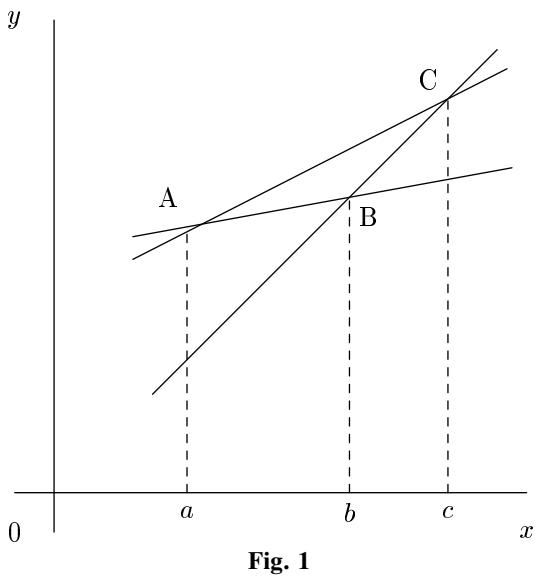
\includegraphics[keepaspectratio]{images/part001_7b60909a.jpg}}

\subsection{凸函数的定义}

定义 1. 我们说，有限数值函数 \(f\) （定义在区间 \(\mathrm{I} \subset \mathbf{R}\) 上的）在 \(\mathrm{I}\) 上是凸的，如果不论点 \(x, x'\) （\(\mathrm{I}\) 中的，\((x < x')\) ）如何，每一点 \(\mathrm{M}_z\) （属于图像 \(\mathrm{G}\) ，即 \(f\) 的图像，且满足 \(x \leqslant z \leqslant x'\) 的）都位于线段 \(\mathrm{M}_x\mathrm{M}_{x'}\) 之下（或者，等价地，如果此线段的每一点都位于 \(\mathrm{G}\) 之上）（fig.~2）。

\pandocbounded{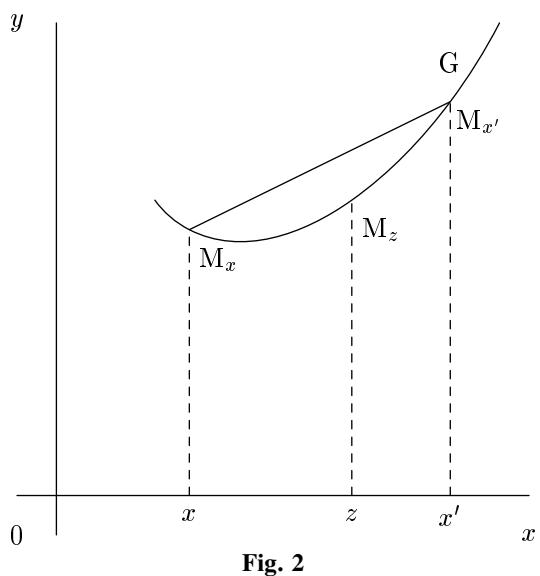
\includegraphics[keepaspectratio]{images/part001_0967d261.jpg}}

考虑到线段的参数表示（Gen.~Top., VI, p.~35），f 在 I 上凸的条件是不等式

\[
f (\lambda x + (1 - \lambda) x ^ {\prime}) \leqslant \lambda f (x) + (1 - \lambda) f (x ^ {\prime})\tag{1}
\]

对 I 的每一对点 \((x, x')\) 及每个 \(\lambda \in [0, 1]\) 成立。

定义 1 等价于：\(\mathbf{R}^2\) 中位于图像 \(G\) （即 \(f\) 的图像）上方的点所成的集是凸的。事实上，这一条件显然足以使 \(f\) 在 I 上凸；它也是必要的，因为若 \(f\) 在 I 上凸，且 \((x,y)\) 、\((x',y')\) 是位于 \(G\) 上方的两点，则有 \(y \geqslant f(x)\) ，\(y' \geqslant f(x')\) ，由此，对 \(0 \leqslant \lambda \leqslant 1\) ，

\[
\lambda y + (1 - \lambda) y ^ {\prime} \geqslant \lambda f (x) + (1 - \lambda) f \left(x ^ {\prime}\right) \geqslant f (\lambda x + (1 - \lambda) x ^ {\prime})
\]

（由 (1)），这表明以 \((x, y)\) 与 \((x', y')\) 为端点的线段的每一点都位于 G 上方。

注. 同样可以看出，严格位于 G 上方的点所成的集是凸的。反之，若此集是凸的，则有

\[
\lambda y + (1 - \lambda) y ^ {\prime} > f (\lambda x + (1 - \lambda) x ^ {\prime})
\]

对 \(0 \leqslant \lambda \leqslant 1\) 及 \(y > f(x)\) 、\(y' > f(x')\) 成立；在此公式中让 \(y\) 趋于 \(f(x)\) 、\(y'\) 趋于 \(f(x')\) ，便得出 \(f\) 是凸的。

例。1) 每个（实）仿射线性函数 \(ax + b\) 在 \(\mathbf{R}\) 上都是凸的。

\begin{enumerate}
\def\labelenumi{\arabic{enumi})}
\setcounter{enumi}{1}
\tightlist
\item
  函数 \(x^{2}\) 在 \(\mathbf{R}\) 上是凸的，因为有
\end{enumerate}

\[
\lambda x ^ {2} + (1 - \lambda) x ^ {\prime 2} - \left(\lambda x + (1 - \lambda) x ^ {\prime}\right) ^ {2} = \lambda (1 - \lambda) (x - x ^ {\prime}) ^ {2} \geqslant 0
\]

对 \(0 \leqslant \lambda \leqslant 1\) 。

\begin{enumerate}
\def\labelenumi{\arabic{enumi})}
\setcounter{enumi}{2}
\tightlist
\item
  函数 \(|x|\) 在 \(\mathbf{R}\) 上是凸的，因为
\end{enumerate}

\[
\left| \lambda x + (1 - \lambda) x ^ {\prime} \right| \leqslant \lambda | x | + (1 - \lambda) \left| x ^ {\prime} \right|
\]

对 \(0 \leqslant \lambda \leqslant 1\) 。

显然，若 \(f\) 在 \(\mathbf{I}\) 上凸，则它在任何区间 \(\mathbf{J} \subset \mathbf{I}\) 上的限制在 \(\mathbf{J}\) 上凸。

设 \(f\) 是 \(I\) 上的凸函数，\(x, x'\) 是 \(I\) 中两点，满足 \(x < x'\) ；若 \(z \in I\) 在 \([x, x']\) 之外，则 \(M_z\) 位于直线 \(D\) （联结 \(M_x\) 与 \(M_{x'}\) 的）上方；这是引理的直接推论。

由此推出：若 z 是满足 \(x < z < x'\) 的点且 \(M_{z}\) 位于线段 \(M_{x}M_{x'}\) 上，则对任何别的点 \(z'\) （满足 \(x < z' < x'\) 的），点 \(M_{z'}\) 也位于线段 \(M_{x}M_{x'}\) 上，因为由上所述 \(M_{z'}\) 同时位于此线段的上方和下方；换句话说，此时 f 在 \([x, x']\) 上等于一个仿射线性函数。

定义 2. 我们说，有限实函数 \(f\) （定义在区间 \(\mathbf{I} \subset \mathbf{R}\) 上的）在 \(\mathbf{I}\) 上是严格凸的，如果对任意点 \(x, x'\) （\(\mathbf{I}\) 中的， \(x < x'\) ），每一点 \(\mathbf{M}_z\) （属于图像 \(\mathbf{G}\) ，即 \(f\) 的图像，且满足 \(x < z < x'\) 的）都严格位于线段 \(\mathbf{M}_x\mathbf{M}_{x'}\) 之下（或者，等价地，如果此线段的每一点除端点外都严格位于 \(\mathbf{G}\) 之上）。

换句话说，必须有不等式

\[
f (\lambda x + (1 - \lambda) x ^ {\prime}) <   \lambda f (x) + (1 - \lambda) f (x ^ {\prime})\tag{2}
\]

对 I 的每一对不同的点 \((x, x')\) 及每个 \(\lambda\) （满足 \(0 < \lambda < 1\) 的）成立。

定义 2 之前的那些说明表明：为使凸函数 f 在 I 上严格凸，当且仅当不存在包含在 I 中的（不退化为一点的）区间使得 f 在其上的限制是仿射线性的。

在上面的例子中，第一个和第三个不是严格凸的；另一方面，\(x^2\) 在 \(\mathbf{R}\) 上严格凸；类似的计算表明 \(1 / x\) 在 \(]0, +\infty[\) 上严格凸。

命题 1. 设 \(f\) 是有限实函数，在区间 \(\mathbf{I} \subset \mathbf{R}\) 上凸（相应地，严格凸）。对每一家族 \((x_i)_{1 \leqslant i \leqslant p}\) （由 \(p \geqslant 2\) 个属于 \(\mathbf{I}\) 的不同的点组成），及每一家族 \((\lambda_i)_{1 \leqslant i \leqslant p}\) （由 \(p\) 个实数组成，满足 \(0 < \lambda_i < 1\) 且 \(\sum_{i=1}^{p} \lambda_i = 1\) ），我们有

\[
f \left(\sum_ {i = 1} ^ {p} \lambda_ {i} x _ {i}\right) \leqslant \sum_ {i = 1} ^ {p} \lambda_ {i} f (x _ {i})\tag{3}
\]

（相应地，

\[
f \left(\sum_ {i = 1} ^ {p} \lambda_ {i} x _ {i}\right) <   \sum_ {i = 1} ^ {p} \lambda_ {i} f (x _ {i})).\tag{4}
\]

由于该命题（就凸函数而言）在 \(p = 2\) 时归结为不等式 (1)，我们对 \(p > 2\) 用归纳法论证。数 \(\mu = \sum_{i=1}^{p-1} \lambda_i\) 为 \(> 0\) ；立即可以看出，若 \(a\) 与 \(b\) 是诸 \(x_i\) 中最小者和最大者，则 \(a \leqslant \sum_{i=1}^{p-1} \lambda_i x_i / \sum_{i=1}^{p-1} \lambda_i \leqslant b\) ；换句话说，点 \(x = \frac{1}{\mu} \sum_{i=1}^{p-1} \lambda_i x_i\) 属于 I，且归纳假设蕴含 \(\mu f(x) \leqslant \sum_{i=1}^{p-1} \lambda_i f(x_i)\) ；此外，由 (1) 我们有

\[
f \left(\sum_ {i = 1} ^ {p} \lambda_ {i} x _ {i}\right) = f (\mu x + (1 - \mu) x _ {p}) \leqslant \mu f (x) + (1 - \mu) f (x _ {p}) \leqslant \sum_ {i = 1} ^ {p} \lambda_ {i} f (x _ {i}).
\]

对严格凸函数，从不等式 (2) 出发，同样论证。

我们说有限实函数 \(f\) 在 I 上是凹的（相应地，严格凹的），如果 \(-f\) 在 I 上是凸的（相应地，严格凸的）。这等价于说，对 I 的每一对不同的点 \((x, x')\) 及每个 \(\lambda\) （满足 \(0 < \lambda < 1\) 的），有

\[
f (\lambda x + (1 - \lambda) x ^ {\prime}) \geqslant \lambda f (x) + (1 - \lambda) f (x ^ {\prime})
\]

\[
(\text { resp. } f (\lambda x + (1 - \lambda) x ^ {\prime}) > \lambda f (x) + (1 - \lambda) f (x ^ {\prime})).
\]

\subsection{凸函数族}

命题 2. 设 \(f_{i}\) （ \(1 \leqslant i \leqslant p\) ）是 \(p\) 个凸函数（定义在区间 \(\mathbf{I} \subset \mathbf{R}\) 上的），\(c_{i}\) （ \(1 \leqslant i \leqslant p\) ）是 \(p\) 个任意正数；则函数 \(f = \sum_{i=1}^{p} c_{i} f_{i}\) 在 \(\mathbf{I}\) 上凸。此外，若对至少一个指标 \(j\) ，函数 \(f_{j}\) 在 \(\mathbf{I}\) 上严格凸，且 \(c_{j} > 0\) ，则 \(f\) 在 \(\mathbf{I}\) 上严格凸。

把不等式 (1)（相应地，(2)）应用于每个 \(f_{i}\) ，把关于 \(f_{i}\) 的不等式乘以 \(c_{i}\) ，然后逐项相加，便立即得出结论。

命题 3. 设 \((f_{\alpha})\) 是区间 \(\mathbf{I} \subset \mathbf{R}\) 上的一族凸函数；若此族的上包络 \(g\) 在 \(\mathbf{I}\) 的每一点处有限，则 \(g\) 在 \(\mathbf{I}\) 上凸。

事实上，位于 g 的图像上方的点 \((x, y) \in \mathbf{R}^{2}\) 所成的集是由位于诸函数 \(f_{\alpha}\) 中每一个的图像上方的点所成的凸集之交；因此它是凸的。

命题 4. 设 H 是区间 \(I \subset R\) 上的一集凸函数；若 F 是 H 上的一个滤子，它在 I 上逐点收敛于一个有限实函数 \(f_{0}\) ，则此函数在 I 上凸。

为看出这一点，只需在不等式 (1) 中沿 F 取极限。

\subsection{凸函数的连续性与可导性}

命题 5. 为使实值有限函数 f 在区间 I 上是凸的（相应地，严格凸的），必须且只需：对一切 \(a \in I\)，梯度

\[
p (\mathbf {M} _ {a} \mathbf {M} _ {x}) = \frac {f (x) - f (a)}{x - a}
\]

在 I ∩ ∁\{a\} 上是 x 的递增（相应地，严格递增）函数。

本命题是定义 1 和定义 2 以及 I, p.~23 中的引理的直接推论。

命题 6. 设 \(f\) 是区间 \(\mathbf{I} \subset \mathbf{R}\) 上的实值有限凸函数。那么，在每个内点 \(a\)（属于 \(\mathbf{I}\)）处，函数 \(f\) 连续，具有有限的右导数与左导数，并且 \(f_g'(a) \leqslant f_d'(a)\)。

事实上，对 \(x \in I\) 与 \(x > a\)，函数 \(x \mapsto \frac{f(x) - f(a)}{x - a}\) 递增（命题 5）且有下界，因为若 \(y < a\) 与 \(y \in I\)，就有

\[
\frac {f (y) - f (a)}{y - a} \leqslant \frac {f (x) - f (a)}{x - a}\tag{5}
\]

（依命题 5）；因此这个函数在点 \(a\) 处有有限的右极限；换言之，\(f_d'(a)\) 存在且有限；再者，在 (5) 中令 \(x\) 趋于 \(a\)（\(x > a\)），便得到

\[
\frac {f (y) - f (a)}{y - a} \leqslant f _ {d} ^ {\prime} (a)\tag{6}
\]

对一切属于 I 的 \(y < a\) 成立。同理可证 \(f_{g}^{\prime}(a)\) 存在，且

\[
f _ {d} ^ {\prime} (a) \leqslant \frac {f (x) - f (a)}{x - a}\tag{7}
\]

对 \(x \in I\) 以及 x \textgreater{} a 成立。在这最后一个不等式中令 x 趋于 \(a (x > a)\)，就得到 \(f_{g}^{\prime}(a) \leqslant f_{d}^{\prime}(a)\)。点 a 处左导数与右导数的存在性显然保证 f 在该点连续。

推论 1. 设 \(f\) 是 I 上的凸（相应地，严格凸）函数；若 \(a\) 与 \(b\) 是 I 的两个内点且 \(a < b\)，则有（图~3）

\pandocbounded{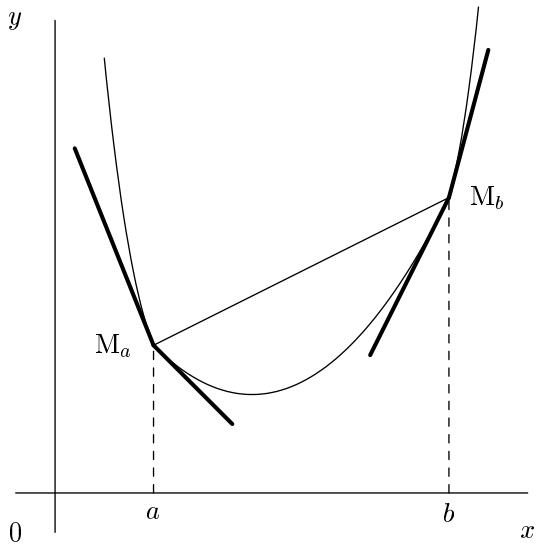
\includegraphics[keepaspectratio]{images/part001_a227d9e4.jpg}}\\
图 3

\[
f _ {d} ^ {\prime} (a) \leqslant \frac {f (b) - f (a)}{b - a} \leqslant f _ {g} ^ {\prime} (b)\tag{8}
\]

（相应地，

\[
f _ {d} ^ {\prime} (a) <   \frac {f (b) - f (a)}{b - a} <   f _ {g} ^ {\prime} (b)).\tag{9}
\]

二重不等式 (8) 由 (6) 与 (7) 经简单的记号改动而得。另一方面，若 \(f\) 严格凸，且 \(c\) 使得 \(a < c < b\)，则由 (8) 与命题 5 得

\[
f _ {d} ^ {\prime} (a) \leqslant \frac {f (c) - f (a)}{c - a} <   \frac {f (b) - f (a)}{b - a} <   \frac {f (b) - f (c)}{b - c} \leqslant f _ {g} ^ {\prime} (b)
\]

由此得 (9)。

推论 2. 若 f 在 I 上是凸的（相应地，严格凸的），则 \(f_{d}^{\prime}\) 与 \(f_{g}^{\prime}\) 在 I 的内部递增（相应地，严格递增）；I 中使 f 不可导的点所成的集是可数的，并且 \(f_{d}^{\prime}\) 与 \(f_{g}^{\prime}\) 在 f 可导的每一点处连续。

第一部分立即由 (8)（相应地，(9)）以及不等式

\[
f _ {g} ^ {\prime} (a) \leqslant f _ {d} ^ {\prime} (a).
\]

得出。另一方面，设 E 为 I 中使 f 不可导的内点 x 所成的集（即 \(f_{g}^{\prime}(x) < f_{d}^{\prime}(x)\)）。对每个 \(x \in E\)，设 \(J_{x}\) 为开区间 \(]f_{g}^{\prime}(x), f_{d}^{\prime}(x)[;\)；由 (8) 可知，若 x 与 y 是 E 中满足 x \textless{} y 的两点，则 u \textless{} v 对一切 \(u \in J_{x}\) 与一切 \(v \in J_{y}\) 成立；换言之，当 x 跑遍 E 时，非空开区间 \(J_{x}\) 两两不相交；这样的区间所成的集因此是可数的，从而 E 也是可数的。最后，\(f_{d}^{\prime}\)（相应地，\(f_{g}^{\prime}\)）递增，故它在 I 的每个内点 x 处都有右极限与左极限；于是 I, p.~18 的命题 6 表明，\(f_{d}^{\prime}\)（相应地，\(f_{g}^{\prime}\)）在点 x 处的右极限等于 \(f_{d}^{\prime}(x)\)，而其左极限等于 \(f_{g}^{\prime}(x)\)；由此即得推论的最后一部分。

设 \(f\) 是 \(I, a\) 上的凸函数，\(I\) 为其一个内点，\(D\) 为过点 \(M_a\) 的一条直线，其方程为 \(y - f(a) = \alpha(x - a)\)。由不等式 (8) 可知，若 \(f_g'(a) \leqslant \alpha \leqslant f_d'(a)\)，则图像 \(G\) 的每一点都位于 \(D\) 之上；并且若 \(f\) 严格凸，则 \(M_a\) 是 \(D\) 与 \(G\) 公有的唯一点；我们称 \(D\) 是 \(G\) 在点 \(M_a\) 处的一条支撑直线。反之，若 \(G\) 位于 \(D\) 之上，则 \(f(x) - f(a) \geqslant \alpha(x - a)\) 对每个 \(x \in I\) 成立，由此 \(\frac{f(x) - f(a)}{x - a} \geqslant \alpha\) 对 \(x > a\) 成立，\(\frac{f(x) - f(a)}{x - a} \leqslant \alpha\) 对 \(x < a\) 成立；在这些不等式中令 \(x\) 趋于 \(a\)，便得 \(f_g'(a) \leqslant \alpha \leqslant f_d'(a)\)。

特别地，若 \(f\) 在点 \(a\) 处可导，则 \(G\) 在点 \(M_a\) 处只有唯一一条支撑直线，即 \(G\) 在 \(M_a\) 处的切线。

注记。若 \(f\) 是开区间 \(I\) 上的严格凸函数，则 \(f_d'\) 在 \(I\) 上严格递增，于是根据 \(I\), p.~13 的命题 2，有三种可能的情形：

\(1^{\circ} f\) 在 I 上严格递减；

\(2^{\circ}\) f 在 I 上严格递增；

\(3^{\circ}\) 存在 \(a \in \mathrm{I}\)，使 \(f\) 对 \(x \leqslant a\) 严格递减，而对 \(x \geqslant a\) 严格递增。

当 \(f\) 在 \(I\) 上是凸的但非严格凸时，\(f\) 可以在含于 \(I\) 的某个区间上取常值；设 \(J = ]a, b[\) 为使 \(f\) 取常值的最大开区间（换言之，使 \(f_{d}^{\prime}(x)=0\) 的区间的内部）；那么 f 在由点 \(x\in I\)（满足 \(x\leqslant a\)）所成的区间上（若它存在）严格递减，在由点 \(x\in I\)（满足 \(x\geqslant b\)）所成的区间上（若它存在）严格递增。

在所有情形中都可以看出，\(f\) 在 I 的左端点处（在 \(\overline{\mathbf{R}}\) 中）具有右极限，在右端点处具有左极限；这些极限可以是有限的或无限的（参见~I, p.~46, 习题 5, 6 与 7）。在用语从宽的意义下，人们有时把取值于 \(\overline{\mathbf{R}}\)、在 I 的内部等于 \(f\) 且由连续性延拓到 I 的端点的连续函数说成是在 \(\overline{\mathbf{I}}\) 上凸的。

\subsection{凸性判别法}

命题 7. 设 f 是定义在区间 \(I \subset R\) 上的实值有限函数。为使 f 在 I 上是凸的，必须且只需：对 I 中满足 a \textless{} b 的每一对数 a, b，以及对每个实数 \(\mu\)，函数 \(f(x) + \mu x\) 都在点 a, b 之一处取得它在 \([a, b]\) 上的上确界。

此条件是必要的；事实上，由于 \(\mu x\) 在 \(\mathbf{R}\) 上凸，函数 \(f(x) + \mu x\) 在 I 上凸；因此可以只限于 \(\mu = 0\) 的情形。此时，对

\[
x = \lambda a + (1 - \lambda) b \quad (0 \leqslant \lambda \leqslant 1),
\]

有

\[
f (x) \leqslant \lambda f (a) + (1 - \lambda) f (b) \leqslant \operatorname{Max} (f (a), f (b)).
\]

此条件是充分的。取 \(\mu = -\frac{f(b) - f(a)}{b - a}\) 并设 \(g(x) = f(x) + \mu x\)；有 \(g(a) = g(b)\)，因此 \(g(x) \leqslant g(a)\) 对一切 \(x \in [a, b]\) 成立，并且可以立即验证这个不等式等价于把 (1) 中的 \(z\) 换成 \(a\)、\(x'\) 换成 \(b\) 所得的不等式。

命题 8. 为使实值有限函数 f 在开区间 \(I \subset R\) 上是凸的（相应地，严格凸的），必须且只需：它在 I 上连续，在此区间的某个可数子集相对于 I 的余集 B 的每一点处有导数，并且该导数在 B 上递增（相应地，严格递增）。

由命题 6 及其推论 2（I, p.~27），此条件是必要的；我们来证明它是充分的。因此假设 \(f'\) 在 B 上递增，而 \(f\) 不是凸的；于是存在（I, p.~27, 命题 5）I 的三个点 \(a, b, c\)，使得 \(a < c < b\) 且 \(\frac{f(c) - f(a)}{c - a} > \frac{f(b) - f(c)}{b - c}\)；但由中值定理（I, p.~14, 定理 1）有

\[
\frac {f (c) - f (a)}{c - a} \leqslant \sup _ {x \in \mathrm{B}, a <   x <   c} f ^ {\prime} (x) \quad \text { and } \quad \frac {f (b) - f (c)}{b - c} \geqslant \inf _ {x \in \mathrm{B}, c <   x <   b} f ^ {\prime} (x).
\]

于是有 \(\sup_{x\in \mathbf{B},a < x < c}f'(x) > \inf_{x\in \mathbf{B},c < x < b}f'(x)\)，这与 \(f'\) 在 B 上递增的假设矛盾。

若现在假设 \(f'\) 在 B 上严格递增，则 \(f\) 是凸的，且不可能在含于 I 的任何开区间上等于一个仿射线性函数，因为否则 \(f'\) 将在该区间上取常值，与假设矛盾。

推论。设 \(f\) 是区间 \(\mathbf{I} \subset \mathbf{R}\) 上的实值有限函数，连续且两次可导；为使 \(f\) 在 \(\mathbf{I}\) 上凸，必须且只需 \(f''(x) \geqslant 0\) 对一切 \(x \in \mathbf{I}\) 成立；为使 \(f\) 在 \(\mathbf{I}\) 上严格凸，必须且只需前述条件成立，并且使点 \(x \in \mathbf{I}\)（在其处 \(f''(x) > 0\)）所成的集在 \(\mathbf{I}\) 中稠密。

这由前一命题以及 I, p.~14 的推论立得。

例。*在区间 {]}0, +∞{[} 上，函数 \(x^r\)（r 为任意实数）的二阶导数等于 \(r(r - 1)x^{r - 2}\)；因此当 \(r > 1\) 或 \(r < 0\) 时它严格凸，而当 \(0 < r < 1\) 时严格凹。*

为了能表述凸性的另一个判别法，我们作如下定义：给定定义在区间 \(I \subset R\) 上的实值有限函数的图像 G 以及 I 的一个内点 a，则称过 \(M_{a} = (a, f(a))\) 的直线 D 局部在 G 上方（相应地，局部在 G 下方），若存在 a 的邻域 \(V \subset I\)，使 D 的每个含于 \(V \times R\) 的点都在 G 之上（相应地，之下）；则称 D 在点 \(M_{a}\) 处局部位于 G 上，若存在 a 的邻域 \(V \subset I\)，使 D 与 \(V \times R\) 的交等同于 G 与 \(V \times R\) 的交（换言之，若 D 同时局部在 G 上方且局部在 G 下方）。

命题 9. 设 f 是开区间 \(I \subset R\) 上的上半连续的实值有限函数。为使 f 在 I 上凸，必须且只需：对 f 的图像 G 的每个点 \(M_{x}\)，在该点处局部在 G 上方的每条直线都局部位于 G 上（在点 \(M_{x}\) 处）。

此条件是必要的：事实上，若 \(f\) 在 \(I\) 上凸，则在点 \(\mathbf{M}_a\)（属于 \(G\)，即 \(f\) 的图像）处都存在一条直线 \(\Delta\)，它支撑 \(G\)；而 \(\Delta\) 位于 \(G\) 之下，故更加局部位于 \(G\) 之下（I, p.~29）；若一条直线 \(D\) 局部在 \(G\) 之上（在点 \(\mathbf{M}_a\) 处），它就局部在 \(\Delta\) 之上，从而必与 \(\Delta\) 重合，因而局部位于 \(G\) 上（在点 \(\mathbf{M}_a\) 处）。

此条件是充分的。事实上，设它成立，并设 \(f\) 在 I 上不凸；于是存在 I 的两个点 \(a, b\)（\(a < b\)），使得有 G 的点 \(\mathbf{M}_x\) 严格位于线段 \(\mathbf{M}_a\mathbf{M}_b\) 之上（图~4）。换言之，函数 \(g(x) = f(x) - f(a) - \frac{f(b) - f(a)}{b - a} (x - a)\) 取值 \(>0\) 于 {[}a, b{]} 上；由于 \(g\) 在这个紧区间上有限且上半连续，它的上确界 \(k\)（在 {[}a, b{]} 上）有限，并且 \(>0\)，而且

\pandocbounded{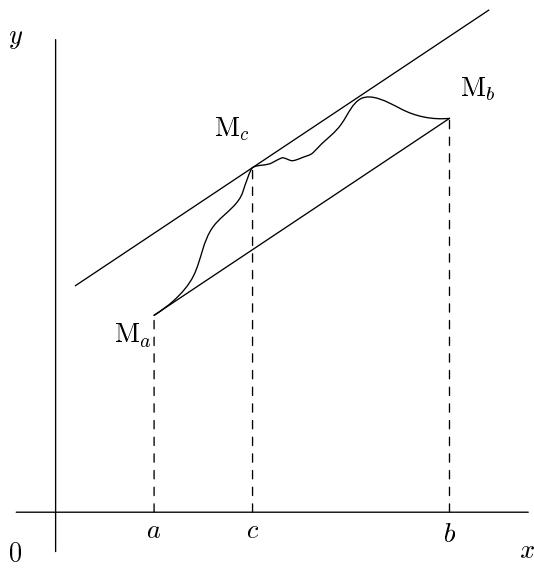
\includegraphics[keepaspectratio]{images/part001_3bcb0893.jpg}}\\
图 4

集 \(\overline{g}(k)\) 是闭的且非空（Gen.~Top., IV, p.~361, 定理 3 与命题 1）。设 c 是 \(\overline{g}(k)\) 的下确界；我们有 a \textless{} c \textless{} b，并且在点 \(M_{c}\) 处方程为 \(y = f(c) + \frac{f(b) - f(a)}{b - a}(x - c)\) 的直线 D 局部在 G 之上；但它在这一点不可能局部位于 G 上，因为对 a \textless{} x \textless{} c 有 \(g(x) < k\)，这表明 \(M_{x}\) 严格位于 D 之下。这就使我们得到矛盾，从而命题得证。

推论 1. 设 \(f\) 是定义在开区间 \(\mathbf{I} \subset \mathbf{R}\) 上且在 \(\mathbf{I}\) 上上半连续的实值有限函数；为使它在 \(\mathbf{I}\) 上凸，必须且只需：对一切 \(x \in \mathbf{I}\)，存在 \(\varepsilon > 0\)，使得关系 \(|h| \leqslant \varepsilon\) 蕴涵

\[
f (x) \leqslant \frac {1}{2} (f (x + h) + f (x - h)).
\]

我们只需证明此条件是充分的。事实上，若在 f 的图像 G 的某个点 \(M_{a}\) 处一条直线 D 局部在 G 之上，则它在该点处局部位于 G 上；因为若不然，例如，将有一个点 \(M_{a+h}\) 严格位于 D 之下，而一个点 \(M_{a-h}\) 位于 D 之下；于是线段 \(M_{a-h}M_{a+h}\) 的中点将严格位于 D 之上（图~5），而依假设，\(M_{a}\) 更加将严格位于 D 之下，这是荒谬的。

\pandocbounded{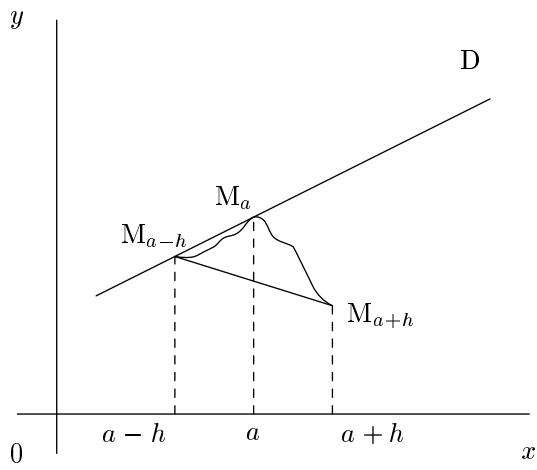
\includegraphics[keepaspectratio]{images/part001_b7dc5930.jpg}}\\
图 5

推论 2. 设 \(f\) 是定义在开区间 \(\mathrm{I} \subset \mathbf{R}\) 上的实值有限函数。若对每个点 \(x \in \mathrm{I}\) 都存在一个开区间 \(\mathrm{J}_x \subset \mathrm{I}\)，它包含 \(x\)，使 \(f\) 在 \(\mathrm{J}_x\) 上的限制在 \(\mathrm{J}_x\) 上凸，则 \(f\) 在 \(\mathrm{I}\) 上凸。

显然 \(f\) 满足命题 9 的判别法。

\setcounter{exercisegroup}{0}
\refstepcounter{exercisegroup}
\section*{第 \S\arabic{exercisegroup} 节习题}
\phantomsection
\addcontentsline{toc}{section}{第 \protect\S\arabic{exercisegroup} 节习题}

\begin{enumerate}
\def\labelenumi{\arabic{enumi})}
\tightlist
\item
  设 \(f\) 是定义在区间 \(I \subset \mathbf{R}\) 上的实变向量函数，在内点 \(x_0\)（\(I\) 的）处可导。证明商
\end{enumerate}

\[
\frac {f (x _ {0} + h) - f (x _ {0} - k)}{h + k}
\]

趋于 \(f'(x_0)\)（当 \(h\) 与 \(k\) 保持取值 \(> 0\) 而趋于 0 时）。逆命题。

*证明函数 \(f\)——等于 \(x^2 \sin 1/x\)（对 \(x \neq 0\)）且等于 0（对 \(x = 0\)）——处处可导，但 \((f(y) - f(z)) / (y - z)\) 并不趋于 \(f'(0)\)（当 \(y\) 与 \(z\) 在保持互异且 \(>0_*\) 的条件下趋于 0 时）。

\begin{enumerate}
\def\labelenumi{\arabic{enumi})}
\setcounter{enumi}{1}
\tightlist
\item
  在区间 I = {[}0, 1{]} 上，我们归纳地定义一个连续实函数序列 \((f_{n})\) 如下：取 \(f_{0}(x) = x\)；对每个整数 \(n \geqslant 1\)，函数 \(f_{n}\) 在 \(3^{n}\) 个区间 \(\left[\frac{k}{3^{n}}, \frac{k+1}{3^{n}}\right]\)（对于 \(0 \leqslant k \leqslant 3^{n}-1\)）的每一个上都是仿射线性的；此外，取
\end{enumerate}

\[
f _ {n + 1} \left(\frac {k}{3 ^ {n}}\right) = f _ {n} \left(\frac {k}{3 ^ {n}}\right)
\]

\[
f _ {n + 1} \left(\frac {k}{3 ^ {n}} + \frac {1}{3 ^ {n + 1}}\right) = f _ {n} \left(\frac {k}{3 ^ {n}} + \frac {2}{3 ^ {n + 1}}\right), f _ {n + 1} \left(\frac {k}{3 ^ {n}} + \frac {2}{3 ^ {n + 1}}\right) = f _ {n} \left(\frac {k}{3 ^ {n}} + \frac {1}{3 ^ {n + 1}}\right).
\]

证明序列 \((f_{n})\) 在 I 上一致收敛于一个连续函数，它在区间 {]}0, 1{[} 的任何点上都没有导数（有限的或无限的）（利用习题 1）。

\begin{enumerate}
\def\labelenumi{\arabic{enumi})}
\setcounter{enumi}{2}
\item
  设 \(\mathcal{C}(\mathrm{I})\) 是定义在紧区间 \(\mathrm{I} = [a,b]\)（含于 \(\mathbf{R}\)）上的连续实值有限函数所成的完备空间，并给 \(\mathcal{C}(\mathrm{I})\) 赋予一致收敛拓扑（Gen.~Top., X, p.~277）。设 A 是 \(\mathcal{C}(\mathrm{I})\) 中由满足如下条件的函数 \(x\) 组成的子集：至少存在一点 \(t\in [a,b[\)（依赖于函数 \(x\)），使函数 \(x\) 在该点有有限的右导数。证明 A 是 \(\mathcal{C}(\mathrm{I})\) 中的瘦集（Gen.~Top., IX, p.~192），因而其余集，即在 \([a,b[\) 的任何一点都没有有限右导数的连续函数所成之集，是 \(\mathcal{C}(\mathrm{I})\) 的一个贝尔子空间（Gen.~Top., IX, p.~192）。（设 \(\mathrm{A}_n\) 是由这样的函数 \(x\in \mathcal{C}(\mathrm{I})\) 组成的集：至少存在 \(t\) 的一个值，满足 \(a\leqslant t\leqslant b - 1 / n\)（且依赖于 \(x\)），使得 \(|x(t') - x(t)|\leqslant n|t' - t|\) 对 \(t'\) 的每个满足 \(t\leqslant t'\leqslant t + 1 / n\) 的值都成立。证明每个 \(\mathrm{A}_n\) 都是 \(\mathcal{C}(\mathrm{I})\) 中的闭的无处稠密集：注意在 \(\mathcal{C}(\mathrm{I})\) 中每个球都含有一个在 \([a,b[\) 上具有有界右导数的函数；另一方面，对每个 \(\varepsilon >0\) 和每个整数 \(m > 0\)，I 上存在一个连续函数，它在 \([a,b[\) 的每一点都有有限右导数，使得对一切 \(t\in [a,b[\) 有 \(|y(t)|\leqslant \varepsilon\) 与 \(|y_r'(t)|\geqslant m\)。）
\item
  设 E 是 R 上的拓扑向量空间，f 是定义在开区间 \(I \subset R\) 上的连续向量函数，并且在 I 的每一点都有右导数与左导数。
\end{enumerate}

\begin{enumerate}
\def\labelenumi{\alph{enumi})}
\item
  设 U 是 E 中的非空开集，A 是 I 中由满足 \(\mathbf{f}_{d}^{\prime}(x) \in \mathrm{U}\) 的点 x 组成的子集。给定数 \(\alpha > 0\)，设 B 是 I 中由这样的点 x 组成的子集：至少存在一个 \(y \in I\)，满足条件 \(x - \alpha \leqslant y < x\) 与 \((\mathbf{f}(x) - \mathbf{f}(y)) / (x - y) \in \mathrm{U}\)；证明集 B 是开集，并且 \(A \cap CB\) 是可数的（注意后一集由与 CB 邻接的区间的左端点组成）。由此推出，由点 \(x \in A\)（满足 \(\mathbf{f}_{g}^{\prime}(x) \notin \overline{\mathbf{U}}\)）所成的集是可数的。
\item
  假设 E 是赋范空间；这时像 \(\mathbf{f}(\mathrm{I})\) 是具有可数基的度量空间，对由 \(\mathbf{f}(\mathrm{I})\) 生成的 E 的闭向量子空间 F 亦然，该子空间包含 \(\mathbf{f}_{d}^{\prime}(\mathrm{I})\) 与 \(\mathbf{f}_{g}^{\prime}(\mathrm{I})\)。由 a) 推出，由点 \(x \in I\)（满足 \(\mathbf{f}_{d}^{\prime}(x) \neq \mathbf{f}_{g}^{\prime}(x)\)）所成的集是可数的。（若 \((\mathrm{U}_{m})\) 是 F 的拓扑的一个可数基，则注意对 F 的两个不同的点 a, b，存在两个不相交的集 \(U_{p}, U_{q}\)，使得 \(a \in U_{p}\) 与 \(b \in U_{q}\)。）
\item
  取 E 为乘积 \(R^{I}\)（即从 I 到 R 的映射所成的空间，赋予简单收敛拓扑），并对每个 \(x \in I\)，用 \(\mathbf{g}(x)\) 表示从 I 到 R 的映射 \(t \mapsto |x - t|\)。证明 g 连续，并且对每个 \(x \in I\) 有 \(\mathbf{g}_{r}'(x) \neq \mathbf{g}_{l}'(x)\)。
\end{enumerate}

\begin{enumerate}
\def\labelenumi{\arabic{enumi})}
\setcounter{enumi}{4}
\tightlist
\item
  设 \(\mathbf{f}\) 是定义在开区间 \(\mathrm{I} \subset \mathbf{R}\) 上、取值于一个赋范空间 \(\mathrm{E}\)（在 \(\mathbf{R}\) 上）中的连续向量函数，并且在 \(\mathrm{I}\) 的每一点处都有右导数。
\end{enumerate}

\begin{enumerate}
\def\labelenumi{\alph{enumi})}
\item
  证明满足如下条件的点 \(x \in \mathrm{I}\) 所成的集——\(\mathbf{f}_d'\) 在 \(x\) 的一个邻域上有界——是 \(\mathrm{I}\) 中的稠密开集（利用 Gen.~Top., IX, p.~194 的定理 2）。
\item
  证明 I 中使 \(\mathbf{f}_d^{\prime}\) 连续的点所成的集是 I 的一个瘦子集的余集（参见~Gen.~Top., IX, p.~255, 习题 21）。
\end{enumerate}

\begin{enumerate}
\def\labelenumi{\arabic{enumi})}
\setcounter{enumi}{5}
\tightlist
\item
  设 \((r_n)\) 是由 {[}0, 1{]} 中的有理数按某个次序排列而成的序列。证明函数 \(f(x) = \sum_{n=0}^{\infty} 2^{-n}(x - r_n)^{1/3}\) 连续且可导
\end{enumerate}

在 \(\mathbf{R}\) 的每个点处，并且在每个点 \(r_n\) 处有无穷导数。（为看出 \(f\) 在点 \(x\)（异于诸 \(r_n\)）处可导，分两种情形讨论，视通项为 \(2^{-n}(x - r_n)^{-2/3}\) 的级数的和是 \(+\infty\) 还是收敛而定；在第二种情形，注意对一切 \(x \neq 0\) 与一切 \(y \neq x\) 有

\[
0 \leqslant (y ^ {1 / 3} - x ^ {1 / 3}) / (y - x) \leqslant 4 / 3 x ^ {2 / 3}).
\]

\begin{enumerate}
\def\labelenumi{\arabic{enumi})}
\setcounter{enumi}{6}
\item
  设 \(f\) 是定义在区间 \(\mathrm{I} \subset \mathbf{R}\) 上的实函数，具有右导数 \(f_d'(x_0) = 0\)（在 \(\mathrm{I}\) 的一点处）；又设 \(\mathbf{g}\) 是定义在 \(y_0 = f(x_0)\) 的一个邻域上的向量函数，在该点处具有右导数与左导数（未必相等）。证明 \(\mathbf{g} \circ f\) 在点 \(x_0\) 处有等于 0 的右导数。
\item
  设 \(f\) 是从 \(\mathbf{R}\) 到其自身的映射，使得集 \(C\)（由 \(\mathbf{R}\) 中使 \(f\) 连续的点组成）在 \(\mathbf{R}\) 中稠密，并且 \(A\)（\(C\) 的余集）也稠密。证明集 \(D\)（由 \(C\) 中使 \(f\) 右可导的点组成）是瘦集。（对每个整数 \(n\)，设 \(E_n\) 是由这样的点 \(a \in \mathbf{R}\) 组成的集：存在两个点 \(x, y\)，使得 \(0 < x - a < 1/n\)、\(0 < y - a < 1/n\) 并且
\end{enumerate}

\[
\frac {f (x) - f (a)}{x - a} - \frac {f (y) - f (a)}{y - a} > 1.
\]

证明 \(E_{n}\) 的内部在 R 中稠密。为此，注意对 R 中每个非空开区间 I 都存在一点 \(b \in I \cap A\)；证明当 a \textless{} b 且 b - a 充分小时有 \(a \in E_{n}\)。

\begin{enumerate}
\def\labelenumi{\arabic{enumi})}
\setcounter{enumi}{8}
\tightlist
\item
  设 \(\mathcal{B}(\mathbf{N})\) 是实数的有界序列 \(\mathbf{x} = (x_n)_{n\in \mathbb{N}}\) 所成的空间，赋予范数 \(\| \mathbf{x}\| = \sup |x_n|\)；给出连续映射 \(t\mapsto \mathbf{f}(t) = (f_n(t))_{n\in \mathbb{N}}\)（从 \(\mathbf{R}\) 到 \(\mathcal{B}(\mathbf{N})\) 中）的一个例子，使得每个函数 \(f_{n}\) 在 \(t = 0\) 处可导，但 \(\mathbf{f}\) 在该点不可导。
\end{enumerate}

\setcounter{exercisegroup}{1}
\refstepcounter{exercisegroup}
\section*{第 \S\arabic{exercisegroup} 节习题}
\phantomsection
\addcontentsline{toc}{section}{第 \protect\S\arabic{exercisegroup} 节习题}

\begin{enumerate}
\def\labelenumi{\arabic{enumi})}
\item
  设 \(f\) 是定义在开区间 \(I = ]a, b[\)（含于 \(R\)）上且左连续的实函数；假设在 \(B\)（\(I\) 中 \(I\) 的一个可数子集的余集）的所有点上，函数 \(f\) 向右递增，也就是说，在每个点 \(x \in B\) 处存在 \(y\)，使得 \(x < y \leqslant b\) 并且对一切 \(z\)（满足 \(x \leqslant z < y\)）有 \(f(x) \leqslant f(z)\)。证明 \(f\) 在 \(I\) 上递增（按命题 2 的方式论证）。
\item
  在 p 进数域 \(Q_{p}\)（Gen.~Top., III, p.~322, 习题 23）中，每个 p 进整数 \(x \in Z_{p}\) 都具有形如 \(x = a_{0} + a_{1}p + \cdots + a_{n}p^{n} + \cdots\) 的唯一展开，其中诸 \(a_{j}\) 是使对每个 j 有 \(0 \leqslant a_{j} \leqslant p - 1\) 的有理整数。对每个 \(z \in Z_{p}\)，令
\end{enumerate}

\[
f (x) = a _ {0} + a _ {1} p ^ {2} + \dots + a _ {n} p ^ {2 n} + \dots ;
\]

证明在 \(Z_{p}\) 上，f 是连续函数，它在任何点的任何邻域上都不取常值，却在每一点都有等于 0 的导数。

\begin{enumerate}
\def\labelenumi{\arabic{enumi})}
\setcounter{enumi}{2}
\tightlist
\item
  \begin{enumerate}
  \def\labelenumii{\alph{enumii})}
  \tightlist
  \item
    设 K 是三分康托集（Gen.~Top., IV, p.~338），设 \(I_{n,p}\) 是 K 的 \(2^{n}\) 个长度为 \(1/3^{n+1}\)（\(1 \leqslant p \leqslant 2^{n}\)）的邻接区间，而 \(K_{n,p}\) 是 \(2^{n+1}\) 个长度为 \(1/3^{n+1}\) 的闭区间，其并是诸 \(I_{m,p}\)（对 \(m \leqslant n\)）之并的余集。设 \(\alpha\) 是使 \(1 < \alpha < 3/2\) 成立的数；对每个 n，用 \(f_{n}\) 表示 {[}0, 1{]} 上的连续递增函数，它在 x = 0 处等于 0，在每个区间 \(I_{m,p}\)（对 \(m \leqslant n\)）上取常值，在每个区间 \(K_{n,p}\)（\(1 \leqslant p \leqslant 2^{n+1}\)）上是仿射线性的，并且在这些后一区间的每一个的内部满足 \(f_{d}'(x) = \alpha^{n+1}\)。证明通项为 \(f_{n}\) 的级数在 {[}0, 1{]} 上一致收敛，其和是一个函数 f，它在 {[}0, 1{[} 中处处具有右导数（有限或否），并且 \(f_{r}'(x) = +\infty\) 在 K 的每个异于诸邻接区间 \(I_{n,p}\) 之左端点的点处成立。
  \end{enumerate}
\end{enumerate}

\begin{enumerate}
\def\labelenumi{\alph{enumi})}
\setcounter{enumi}{1}
\tightlist
\item
  设 g 是 \([0, 1]\) 到其自身上的连续递增映射，在每个区间 \(I_{n,p}\) 上取常值（Gen.~Top., IV, p.~403, 习题 9）。若 \(h = f + g\)，证明 h 具有等于 \(f_{d}^{\prime}(x)\) 的右导数（在 \([0, 1]\) 的每个点 x 处）。
\end{enumerate}

\begin{enumerate}
\def\labelenumi{\arabic{enumi})}
\setcounter{enumi}{3}
\tightlist
\item
  设 \(f\) 是实值有限函数，在紧区间 \([a, b]\)（含于 \(\mathbf{R}\)）上连续，并且在开区间 \(]a, b[\) 的每一点都有右导数。设 \(m\) 与 \(M\) 是 \(f_d'\) 在 \(]a, b[\) 上的下确界与上确界（有限或否）。
\end{enumerate}

\begin{enumerate}
\def\labelenumi{\alph{enumi})}
\item
  证明当 x 与 y 跑遍 {]}a, b{[} 而保持 \(x \neq y\) 时，\((f(x) - f(y))/(x - y)\) 的值所成的集包含 {]}m, M{[} 且含于 {[}m, M{]}。（归结为证明：若 \(f_{d}^{\prime}\) 在 {]}a, b{[} 的两点 c, d 处取异号的两个值（其中 c \textless{} d），则存在区间 {]}c, d{[} 的两个不同的点，使 f 在其上取同一个值。）
\item
  若进一步 f 在 \(]a\) , b{[} 的每一点都有左导数，则 \(f_{d}^{\prime}\) 与 \(f_{g}^{\prime}\) 在 \(]a\) , b{[} 上的下确界（相应地，上确界）相等。
\item
  由此推出：若 \(f\) 在 \(]a, b[\) 上可导，则 \(f'\) 下每个含于 \(]a, b[\) 的区间的像本身是一个区间，从而是连通的（利用 \(a\)）。
\end{enumerate}

\begin{enumerate}
\def\labelenumi{\arabic{enumi})}
\setcounter{enumi}{4}
\item
  设 \(\mathbf{f}\) 是如下定义的从 \(I = [0, 1]\) 到 \(\mathbf{R}^3\) 的向量映射：对 \(0 \leqslant t \leqslant \frac{1}{4}\)，\(\mathbf{f}(t) = (-4t, 0, 0)\)；对 \(\frac{1}{4} \leqslant t \leqslant \frac{1}{2}\)，令 \(\mathbf{f}(t) = (-1, 4t - 1, 0)\)；对 \(\frac{1}{2} \leqslant t \leqslant \frac{3}{4}\)，令 \(\mathbf{f}(t) = (-1, 1, 4t - 2)\)；最后，对 \(\frac{3}{4} \leqslant t \leqslant 1\)，取 \(\mathbf{f}(t) = (4t - 4, 1, 1)\)。证明由集 \(\mathbf{f}_d'(\mathrm{I})\) 生成的凸集不同于 \(\frac{\mathbf{f}(y) - \mathbf{f}(x)}{y - x}\) 的值集（当 \((x, y)\) 跑遍 \(I\) 的互异点对所成之集时）的闭包（参见~习题 \(4a\)））。
\item
  在区间 \(\mathbf{I} = [-1, + 1]\) 上考虑向量函数 \(\mathbf{f}\)，取值于 \(\mathbf{R}^2\)，定义如下：\(\mathbf{f}(t) = (0,0)\)（当 \(-1\leqslant t\leqslant 0\) 时）；
\end{enumerate}

\[
\mathbf {f} (t) = \left(t ^ {2} \sin \frac {1}{t}, t ^ {2} \cos \frac {1}{t}\right)
\]

当 \(0 \leqslant t \leqslant 1\) 时。证明 \(\mathbf{f}\) 在 \([-1, +1[\) 上可导，但这个区间在 \(\mathbf{f}'\) 下的像不是 \(\mathbf{R}^2\) 中的连通集（\(cf.\) 习题 \(4c\)））。

\begin{enumerate}
\def\labelenumi{\arabic{enumi})}
\setcounter{enumi}{6}
\item
  设 f 是定义在开区间 \(I \subset R\) 上、取值于 R 上的赋范空间 E 中的连续向量函数，并且在 I 的每一点都具有右导数。证明 I 中使 f 具有导数的点所成的集是 I 的一个瘦子集的余集（利用 I, p.~36 的习题 5 b) 以及 I, p.~18 的命题 6）。
\item
  在区间 {[}0, 1{]} 上考虑一个两两不相交的开区间族 \((\mathrm{I}_{n,p})\)，归纳地定义如下：整数 \(n\) 取遍一切值 \(\geqslant 0\)；对 \(n\) 的每个值，整数 \(p\) 取值 \(1,2,\ldots ,2^n\)；有 \(\mathrm{I}_{0,1} = ]\frac{1}{3},\frac{2}{3}[\)；若 \(\mathrm{J}_n\) 是区间 \(\mathrm{I}_{m,p}\)（与诸数 \(m\leqslant n\) 相应）之并，则 \(\mathrm{J}_n\) 的余集是 \(2^{n + 1}\) 个两两不相交的闭区间 \(\mathrm{K}_{n,p}\)（\(1\leqslant p\leqslant 2^{n + 1}\)）之并。若 \(\mathrm{K}_{n,p}\) 是一个区间 \([a,b]\)，则取 \(\mathrm{I}_{n + 1,p}\) 为以 \(b - \frac{b - a}{3}\left(1 + \frac{1}{2^n}\right)\) 与 \(b - \frac{b - a}{3.2^n}\) 为端点的开区间。设 E 是完备集，即 {[}0, 1{]} 相对于诸 \(\mathrm{I}_{n,p}\) 之并的余集。在 {[}0, 1{]} 上定义一个连续实函数 \(f\)，它在 {[}0, 1{]} 的每一点都具有右导数，但在 E 的由异于 E 的邻接区间的端点的点组成的不可数子集的每一点处没有左导数（参见~习题 7）。（在 E 上取 \(f(x) = 0\)，并把 \(f\) 在每个区间 \(\mathrm{I}_{n,p}\) 上适当地加以定义，使得对每个 \(x\in \mathrm{E}\)，都存在点 \(y < x\)（不属于 E，任意接近 \(x\)），并且满足 \(\frac{f(y) - f(x)}{y - x} = -1\)。）
\item
  设 \(f\) 与 \(g\) 是两个实值有限函数，在 \([a, b]\) 上连续，都在 \(]a, b[\) 上有有限导数；证明存在 \(c\)，使得 \(a < c < b\)，并且
\end{enumerate}

\[
\left| \begin{array}{c c} f (b) - f (a) & g (b) - g (a) \\ f ^ {\prime} (c) & g ^ {\prime} (c) \end{array} \right| = 0.
\]

¶ 10) 设 \(f\) 与 \(g\) 是两个实值有限函数，严格正、连续且在开区间 I 上可导。证明若 \(f'\) 与 \(g'\) 严格正且 \(f'/g'\) 在 I 上严格递增，则或者 \(f/g\) 在 I 上严格递增，或者存在数 \(c \in I\)，使得 \(f / g\) 对 \(x \leqslant c\) 严格递减而对 \(x \geqslant c\) 严格递增（注意若有 \(f'(x) / g'(x) < f(x) / g(x)\) 则也有

\[
f ^ {\prime} (y) / g ^ {\prime} (y) <   f (y) / g (y)
\]

对一切 y \textless{} x 成立）。

\begin{enumerate}
\def\labelenumi{\arabic{enumi})}
\setcounter{enumi}{10}
\tightlist
\item
  设 \(f\) 是复函数，在开区间 \(I\) 上连续、处处不为零，并且在 \(I\) 的每一点都具有右导数。为使 \(|f|\) 在 \(I\) 上递增，必须且只需 \(\mathcal{R}(f_d' / f) \geqslant 0\) 在 \(I\) 上成立。
\end{enumerate}

¶ 12) 设 \(f\) 是开区间 I 上的可导实函数，\(g\) 是它在 I 上的导数，\([a, b]\) 是含于 I 的紧区间；假设 \(g\) 在开区间 \([a, b]\) 上可导，但在点 \(a\)（相应地，\(b\)）处未必右（相应地，左）连续；证明存在 \(c\)，使得 \(a < c < b\)，并且

\[
g (b) - g (a) = (b - a) g ^ {\prime} (c)
\]

（利用 I, p.~36 的习题 4 c)）。

\begin{enumerate}
\def\labelenumi{\arabic{enumi})}
\setcounter{enumi}{12}
\tightlist
\item
  我们把向量函数 \(\mathbf{f}\) 在一点 \(x_0\)（内于 \(\mathbf{f}\) 的定义区间）处的对称导数定义为：\(\frac{\mathbf{f}(x_0 + h) - \mathbf{f}(x_0 - h)}{2h}\) 当 \(h\) 保持 \(>0\) 而趋于 0 时的极限（当它存在时）。
\end{enumerate}

\begin{enumerate}
\def\labelenumi{\alph{enumi})}
\item
  把 § 1 中对导数建立的运算法则推广到对称导数。
\item
  证明当把“右导数”一词换成“对称导数”时，§ 2 的定理 1 与定理 2 仍然成立。
\end{enumerate}

\begin{enumerate}
\def\labelenumi{\arabic{enumi})}
\setcounter{enumi}{13}
\tightlist
\item
  设 \(\mathbf{f}\) 是定义在紧区间 \(\mathrm{I} = [a, b]\)（含于 \(\mathbf{R}\)）上且连续的向量函数，取值于 \(\mathbf{R}\) 上的一个赋范空间中。假设 \(\mathbf{f}\) 在此区间的某个可数子集 A 相对于 \([a, b[\) 的余集的所有点处都具有右导数。证明存在一点 \(x \in ]a\)、\(b[\cap ∁A\)，使得
\end{enumerate}

\[
\left\| \mathbf {f} (b) - \mathbf {f} (a) \right\| \leqslant \left\| \mathbf {f} _ {d} ^ {\prime} (x) \right\| (b - a).
\]

（用反证法论证，把 \([a, b[\) 分解为三个区间 \([a, t[, [t, t + h[\) 与 \([t + h, b[\)，满足 \(t \notin A\)；若 \(k = \| \mathbf{f}(b) - \mathbf{f}(a)\| / (b - a)\)，则注意当 \(h\) 充分小时有 \(\| \mathbf{f}(t + h) - \mathbf{f}(t)\| < k.h\)，并对其余区间使用 I, p.~15 的定理 2。）

\setcounter{exercisegroup}{2}
\refstepcounter{exercisegroup}
\section*{第 \S\arabic{exercisegroup} 节习题}
\phantomsection
\addcontentsline{toc}{section}{第 \protect\S\arabic{exercisegroup} 节习题}

\begin{enumerate}
\def\labelenumi{\arabic{enumi})}
\tightlist
\item
  在与 I, p.~20 的命题 2 相同的假设下，证明公式
\end{enumerate}

\[
[ \mathbf {f} ^ {(n)}. \mathbf {g} ] = \sum_ {p = 0} ^ {n} (- 1) ^ {p} \binom {n} {p} D ^ {n - p} [ \mathbf {f}. \mathbf {g} ^ {(p)} ].
\]

\begin{enumerate}
\def\labelenumi{\arabic{enumi})}
\setcounter{enumi}{1}
\tightlist
\item
  采用 I, p.~28 的命题 2 的记号，假设关系 \([\mathbf{a}.\mathbf{y}] = 0\)（对一切 \(\mathbf{y} \in \mathrm{F}\)）蕴涵 E 中的 \(\mathbf{a} = 0\)。在这些条件下，若 \(\mathbf{g}_i\)（\(0 \leqslant i \leqslant n\)）是 \(n + 1\) 个取值于 E 的向量函数，定义在 R 的区间 I 上，并且对每个取值于 F、在 I 上 n 次可导的向量函数 f 都恒有
\end{enumerate}

\[
[ \mathbf {g} _ {0}. \mathbf {f} ] + [ \mathbf {g} _ {1}. \mathbf {f} ^ {\prime} ] + \dots + [ \mathbf {g} _ {n}. \mathbf {f} ^ {(n)} ] = 0
\]

则诸函数 \(g_{i}\) 恒为零。

\begin{enumerate}
\def\labelenumi{\arabic{enumi})}
\setcounter{enumi}{2}
\tightlist
\item
  采用习题 2 的记号并对 \([x.y]\) 作同样的假设，设每个函数 \(g_{k}\) 都在 I 上 n 次可导；对每个在 I 上 n 次可导、取值于 F 的函数 f，令
\end{enumerate}

\[
[ \mathbf {g} _ {0}. \mathbf {f} ] - [ \mathbf {g} _ {1}. \mathbf {f} ] ^ {\prime} + [ \mathbf {g} _ {2}. \mathbf {f} ] ^ {\prime \prime} + \dots + (- 1) ^ {n} [ \mathbf {g} _ {n}. \mathbf {f} ] ^ {(n)} = [ \mathbf {h} _ {0}. \mathbf {f} ] + [ \mathbf {h} _ {1}. \mathbf {f} ^ {\prime} ] + \dots + [ \mathbf {h} _ {n}. \mathbf {f} ^ {(n)} ],
\]

这便无歧义地定义了诸函数 \(\mathbf{h}_i\)（\(0 \leqslant i \leqslant n\)）（习题 2）；证明有

\[
[ \mathbf {h} _ {0}. \mathbf {f} ] - [ \mathbf {h}. \mathbf {f} ] ^ {\prime} + [ \mathbf {h} _ {2}. \mathbf {f} ] ^ {\prime \prime} + \dots + (- 1) ^ {n} [ \mathbf {h} _ {n}. \mathbf {f} ] ^ {(n)} = [ \mathbf {g} _ {0}. \mathbf {f} ] + [ \mathbf {g} _ {1}. \mathbf {f} ^ {\prime} ] + \dots + [ \mathbf {g} _ {n}. \mathbf {f} ^ {(n)} ]
\]

恒成立。

\begin{enumerate}
\def\labelenumi{\arabic{enumi})}
\setcounter{enumi}{3}
\tightlist
\item
  设 \(\mathbf{f}\) 是 \(n\) 次可导的向量函数，定义在区间 \(\mathrm{I} \subset \mathbf{R}\) 上。证明对 \(1 / x \in \mathrm{I}\) 恒有
\end{enumerate}

\[
\frac {1}{x ^ {n + 1}} \mathbf {f} ^ {(n)} \left(\frac {1}{x}\right) = (- 1) ^ {n} \mathrm{D} ^ {n} \left(x ^ {n - 1} \mathbf {f} \left(\frac {1}{x}\right)\right)
\]

（对 \(n\) 作归纳论证）。

\begin{enumerate}
\def\labelenumi{\arabic{enumi})}
\setcounter{enumi}{4}
\tightlist
\item
  设 \(u\) 与 \(v\) 是两个 \(n\) 次可导的实函数，定义在区间 \(I \subset \mathbf{R}\) 上。若令 \(D^n(u / v) = (-1)^n w_n / v^{n+1}\)（在使 \(v(x) \neq 0\) 的每一点处），证明
\end{enumerate}

\[
w _ {n} = \left| \begin{array}{c c c c c c} u & v & 0 & 0 & \dots & 0 \\ u ^ {\prime} & v ^ {\prime} & v & 0 & \dots & 0 \\ u ^ {\prime \prime} & v ^ {\prime \prime} & 2 v ^ {\prime} & v & \dots & 0 \\ \dots & \dots & \dots & \dots & \dots & \dots \\ u ^ {(n - 1)} & v ^ {(n - 1)} & \binom {n - 1} {1} v ^ {(n - 2)} & \binom {n - 1} {2} v ^ {(n - 3)} & \dots & v \\ u ^ {(n)} & v ^ {(n)} & \binom {n} {1} v ^ {(n - 1)} & \binom {n} {2} v ^ {(n - 2)} & \dots & \binom {n} {n - 1} v ^ {\prime} \end{array} \right|
\]

（令 \(w = u / v\) 并微分 \(n\) 次关系 \(u = wv\)）。

\begin{enumerate}
\def\labelenumi{\arabic{enumi})}
\setcounter{enumi}{5}
\tightlist
\item
  设 \(\mathbf{f}\) 是定义在开区间 \(\mathrm{I} \subset \mathbf{R}\) 上、取值于赋范空间 \(\mathrm{E}\) 的向量函数。
\end{enumerate}

令 \(\Delta \mathbf{f}(x; h_1) = \mathbf{f}(x + h_1) - \mathbf{f}(x)\)，然后归纳地定义

\[
\Delta^ {p} \mathbf {f} (x; h _ {1}, h _ {2}, \dots , h _ {p - 1}, h _ {p}) = \Delta^ {p - 1} \mathbf {f} (x + h _ {p}; h _ {1}, \dots , h _ {p - 1}) - \Delta^ {p - 1} \mathbf {f} (x; h _ {1}, \dots , h _ {p - 1});
\]

这些函数对每个 \(x \in I\) 都有定义（当诸 \(h_{i}\) 充分小时）。

\begin{enumerate}
\def\labelenumi{\alph{enumi})}
\tightlist
\item
  若函数 \(\mathbf{f}\) 是 \(n\) 次可导的（在点 \(x\) 处；从而是 \(n - 1\) 次可导的，在 \(x\) 的一个邻域上），则有
\end{enumerate}

\[
\lim_{\substack{(h_{1},\ldots ,h_{n})\to (0,\ldots ,0)\\ h_{1}h_{2}\ldots h_{n}\neq 0}}\frac{\varDelta^{n}\mathbf{f}(x;h_{1},\ldots,h_{n})}{h_{1}h_{2}\ldots h_{n}} = \mathbf{f}^{(n)}(x)
\]

（对 n 作归纳论证，并使用中值定理）。

\begin{enumerate}
\def\labelenumi{\alph{enumi})}
\setcounter{enumi}{1}
\tightlist
\item
  若 \(\mathbf{f}\) 在区间 I 上 \(n\) 次可导，则有
\end{enumerate}

\[
\begin{array}{l} \left\| \Delta^ {n} \mathbf {f} (x; h _ {1}, \ldots , h _ {n}) - \mathbf {f} ^ {(n)} (x _ {0}) h _ {1} h _ {2} \ldots h _ {n} \right\| \\ \leqslant | h _ {1} h _ {2} \ldots h _ {n} | \sup \left\| \mathbf {f} ^ {(n)} (x + t _ {1} h _ {1} + \dots + t _ {n} h _ {n}) - \mathbf {f} ^ {(n)} (x _ {0}) \right\| \end{array}
\]

其中上确界是对 \((t_i)\)（满足 \(0 \leqslant t_i \leqslant 1\)，对 \(1 \leqslant i \leqslant n\)）所成的集取的（同样方法）。

\begin{enumerate}
\def\labelenumi{\alph{enumi})}
\setcounter{enumi}{2}
\tightlist
\item
  若 \(f\) 是在 I 上 \(n\) 次可导的实函数，则有
\end{enumerate}

\[
\Delta^ {n} f (x; h _ {1}, h _ {2}, \dots , h _ {n}) = h _ {1} h _ {2} \dots h _ {n} f ^ {(n)} (x + \theta_ {1} h _ {1} + \dots + \theta_ {n} h _ {n})
\]

其中诸数 \(\theta_{i}\) 属于 {[}0, 1{]}（同样方法，利用 I, p.~22 的推论）。

\begin{enumerate}
\def\labelenumi{\arabic{enumi})}
\setcounter{enumi}{6}
\tightlist
\item
  设 \(f\) 是 \(n\) 次可导的实值有限函数（在点 \(x_0\) 处），\(\mathbf{g}\) 是 \(n\) 次可导的向量函数（在点 \(y_0 = f(x_0)\) 处）。设
\end{enumerate}

\[
\begin{array}{l} f (x _ {0} + h) = a _ {0} + a _ {1} h + \dots + a _ {n} h ^ {n} + r _ {n} (h) \\ \mathbf {g} (y _ {0} + k) = \mathbf {b} _ {0} + \mathbf {b} _ {1} k + \dots + \mathbf {b} _ {n} k ^ {n} + \mathbf {s} _ {n} (k) \end{array}
\]

分别是 f 在点 \(x_{0}\) 处与 g 在点 \(y_{0}\) 处的 n 阶泰勒展开。证明 \(n+1\) 项之和（指复合函数 \(g \circ f\) 在点 \(x_{0}\) 处的 n 阶泰勒展开中的）等于下列多项式中次数 \(\leqslant n\) 的项之和

\[
\mathbf {b} _ {0} + \mathbf {b} _ {1} (a _ {1} h + \dots + a _ {n} h ^ {n}) + \mathbf {b} _ {2} (a _ {1} h + \dots + a _ {n} h ^ {n}) ^ {2} + \dots + \mathbf {b} _ {n} (a _ {1} h + \dots + a _ {n} h ^ {n}) ^ {n}.
\]

由此推出下面两个公式：

\begin{enumerate}
\def\labelenumi{\alph{enumi})}
\tightlist
\item
\end{enumerate}

\[
\mathrm{D} ^ {n} (\mathbf {g} (f (x))) = \sum \frac {n !}{m _ {1} ! m _ {2} ! \dots m _ {q} !} \mathbf {g} ^ {(p)} (f (x)) \left(\frac {f ^ {\prime} (x)}{1 !}\right) ^ {m _ {1}} \dots \left(\frac {f ^ {(q)} (x)}{q !}\right) ^ {m _ {q}}
\]

其中求和取遍一切满足如下条件的正整数组 \((m_{i})_{1\leqslant i\leqslant q}\)：

\[
m _ {1} + 2 m _ {2} + \dots + q m _ {q} = n
\]

其中 p 表示和 \(m_{1} + m_{2} + \cdots + m_{q}\)。

\begin{enumerate}
\def\labelenumi{\alph{enumi})}
\setcounter{enumi}{1}
\tightlist
\item
\end{enumerate}

\[
\mathrm{D} ^ {n} (\mathbf {g} (f (x))) = \sum_ {p = 1} ^ {n} \frac {1}{p !}   \mathbf {g} ^ {(p)} (f (x)) \left(\sum_ {q = 1} ^ {p} \binom {p} {q} (- f (x)) ^ {p - q}   \mathrm{D} ^ {n} ((f (x)) ^ {q}\right).
\]

\begin{enumerate}
\def\labelenumi{\arabic{enumi})}
\setcounter{enumi}{7}
\tightlist
\item
  设 \(f\) 是一个 \(n\) 次可导、定义在区间 \(\mathrm{I}\) 上的实函数，设 \(x_{1}, x_{2}, \ldots, x_{p}\) 是 \(\mathrm{I}\) 的互异点，而 \(n_{i}\)（\(1 \leqslant i \leqslant p\)）是 \(p\) 个整数 \(> 0\)，使得
\end{enumerate}

\[
n _ {1} + n _ {2} + \dots + n _ {p} = n.
\]

假设在点 \(x_{i}\) 处，函数 f 连同它的前 \(n_{i}-1\) 阶导数对 \(1 \leqslant i \leqslant p\) 都为零：证明存在一点 \(\xi\)，它内在于包含诸 \(x_{i}\) 的最小区间，并且使得 \(f^{(n-1)}(\xi) = 0\)。

\begin{enumerate}
\def\labelenumi{\arabic{enumi})}
\setcounter{enumi}{8}
\tightlist
\item
  采用与习题 8 相同的记号，设 \(f\) 在 I 上 \(n\) 次可导但别处任意。设 \(g\) 是 \(n - 1\) 次（实系数）多项式，使得在点 \(x_{i}\)（\(1 \leqslant i \leqslant p\)）处，\(g\) 及其前 \(n_{i} - 1\) 阶导数分别等于 \(f\) 及其前 \(n_{i} - 1\) 阶导数。证明我们有
\end{enumerate}

\[
f (x) = g (x) + \frac {(x - x _ {1}) ^ {n _ {1}} (x - x _ {2}) ^ {n _ {2}} \dots (x - x _ {p}) ^ {n _ {p}}}{n !} f ^ {(n)} (\xi)
\]

其中 \(\xi\) 内在于包含诸点 \(x_{i}\)（\(1 \leqslant i \leqslant p\)）与 \(x\) 的最小区间。（对 \(t\) 的函数

\[
f (t) - g (t) - a \frac {(t - x _ {1}) ^ {n _ {1}} (t - x _ {2}) ^ {n _ {2}} \dots (t - x _ {p}) ^ {n _ {p}}}{n !}
\]

应用习题 8，其中 \(a\) 是适当选取的常数。）

\begin{enumerate}
\def\labelenumi{\arabic{enumi})}
\setcounter{enumi}{9}
\tightlist
\item
  设 \(g\) 是定义在 0 的一个邻域上的奇实函数，并且在该邻域上 5 次可导。证明
\end{enumerate}

\[
g (x) = \frac {x}{3} \left(g ^ {\prime} (x) + 2 g ^ {\prime} (0)\right) - \frac {x ^ {5}}{1 8 0} g ^ {(5)} (\xi) \quad (\xi = \theta x, \quad 0 <   \theta <   1)
\]

（与习题 9 相同的方法）。

由此推出：若 \(f\) 是定义在 \([a, b]\) 上且在此区间上 5 次可导的实函数，则

\[
f (b) - f (a) = \frac {b - a}{6} \left[ f ^ {\prime} (a) + f ^ {\prime} (b) + 4 f ^ {\prime} \left(\frac {a + b}{2}\right) \right] - \frac {(b - a) ^ {5}}{2 8 8 0} f ^ {(5)} (\xi)
\]

其中 \(a < \xi < b\)（“辛普森公式”）。

\begin{enumerate}
\def\labelenumi{\arabic{enumi})}
\setcounter{enumi}{10}
\tightlist
\item
  设 \(f_{1}, f_{2}, \ldots, f_{n}\) 与 \(g_{1}, g_{2}, \ldots, g_{n}\) 是 \(2n\) 个在区间 I 上 \(n - 1\) 次可导的实函数。设 \((x_{i})_{1 \leqslant i \leqslant n}\) 是 I 中点的严格递增序列。证明两个行列式
\end{enumerate}

\[
\left| \begin{array}{c c c c} f _ {1} (x _ {1}) & f _ {1} (x _ {2}) & \dots & f _ {1} (x _ {n}) \\ f _ {2} (x _ {1}) & f _ {2} (x _ {2}) & \dots & f _ {2} (x _ {n}) \\ \dots & \dots & \dots & \dots \\ f _ {n} (x _ {1}) & f _ {n} (x _ {2}) & \dots & f _ {n} (x _ {n}) \end{array} \right| \vdots \left| \begin{array}{c c c c} g _ {1} (x _ {1}) & g _ {1} (x _ {2}) & \dots & g _ {1} (x _ {n}) \\ g _ {2} (x _ {1}) & g _ {2} (x _ {2}) & \dots & g _ {2} (x _ {n}) \\ \dots & \dots & \dots & \dots \\ g _ {n} (x _ {1}) & g _ {n} (x _ {2}) & \dots & g _ {n} (x _ {n}) \end{array} \right|
\]

之比等于两个行列式

\[
\left| \begin{array}{c c c c} f _ {1} (\xi_ {1}) & f _ {1} ^ {\prime} (\xi_ {2}) & \dots & f _ {1} ^ {(n - 1)} (\xi_ {n}) \\ f _ {2} (\xi_ {1}) & f _ {2} ^ {\prime} (\xi_ {2}) & \dots & f _ {2} ^ {(n - 1)} (\xi_ {n}) \\ \dots & \dots & \dots & \dots \\ f _ {n} (\xi_ {1}) & f _ {n} ^ {\prime} (\xi_ {2}) & \dots & f _ {n} ^ {(n - 1)} (\xi_ {n}) \end{array} \right|: \left| \begin{array}{c c c c} g _ {1} (\xi_ {1}) & g _ {1} ^ {\prime} (\xi_ {2}) & \dots & g _ {1} ^ {(n - 1)} (\xi_ {n}) \\ g _ {2} (\xi_ {1}) & g _ {2} ^ {\prime} (\xi_ {2}) & \dots & g _ {2} ^ {(n - 1)} (\xi_ {n}) \\ \dots & \dots & \dots & \dots \\ g _ {n} (\xi_ {1}) & g _ {n} ^ {\prime} (\xi_ {2}) & \dots & g _ {n} ^ {(n - 1)} (\xi_ {n}) \end{array} \right|
\]

之比，其中

\[
\xi_ {1} = x _ {1}, \quad \xi_ {1} <   \xi_ {2} <   x _ {2}, \quad \xi_ {2} <   \xi_ {3} <   x _ {3}, \quad \dots , \quad \xi_ {n - 1} <   \xi_ {n} <   x _ {n}
\]

（应用 I, p.~38 的习题 9）。

\(g_{1}(x)=1\)、\(g_{2}(x)=x,\ldots,g_{n}(x)=x^{n-1}\) 的特殊情形。

¶ 12) \(a)\) 设 \(\mathbf{f}\) 是定义在有限区间 \(\mathrm{I} = [-a, + a]\) 上且连续的向量函数，取值于赋范空间 \(\mathrm{E}\)（在 \(\mathbf{R}\) 上）中，并且在 \(\mathrm{I}\) 上两次可导。若令 \(\mathrm{M}_0 = \sup_{x\in \mathrm{I}}\| \mathbf{f}(x)\|\)、\(\mathrm{M}_2 = \sup_{x\in \mathrm{I}}\| \mathbf{f}''(x)\|\)，证明对一切 \(x\in \mathrm{I}\) 有

\[
\left\| \mathbf {f} ^ {\prime} (x) \right\| \leqslant \frac {\mathrm{M} _ {0}}{a} + \frac {x ^ {2} + a ^ {2}}{2 a} \mathrm{M} _ {2}
\]

（把诸差 \(\mathbf{f}(a) - \mathbf{f}(x)\)、\(\mathbf{f}(-a) - \mathbf{f}(x)\) 表出）。

\begin{enumerate}
\def\labelenumi{\alph{enumi})}
\setcounter{enumi}{1}
\tightlist
\item
  由 a) 推出：若 f 是区间 I（有界或否）上的两次可导函数，并且 \(\mathbf{M}_{0} = \sup_{x \in I} \| \mathbf{f}(x) \|\) 与 \(\mathbf{M}_{2} = \sup_{x \in I} \| \mathbf{f}''(x) \|\) 有限，则 \(\mathbf{M}_{1} = \sup_{x \in I} \| \mathbf{f}'(x) \|\) 也有限，并且有：
\end{enumerate}

\[
\mathrm{M} _ {1} \leqslant 2 \sqrt {\mathrm{M} _ {0} \mathrm{M} _ {2}} \quad \text { if   I   has   length } \geqslant 2 \sqrt {\frac {M _ {0}}{\mathrm{M} _ {2}}}
\]

\[
\mathrm{M} _ {1} \leqslant \sqrt {2} \sqrt {\mathrm{M} _ {0} \mathrm{M} _ {2}} \quad \text { if } \mathrm{I} = \mathbf {R}.
\]

证明在这两个不等式中，数 2 与 \(\sqrt{2}\) 分别不能换成更小的数（先考虑仅设 f 具有二阶右导数的情形，并证明此时取 f 为“分段”等于二次多项式的实函数，前述不等式中的两项可以变成相等的）。

\begin{enumerate}
\def\labelenumi{\alph{enumi})}
\setcounter{enumi}{2}
\tightlist
\item
  由 \(b)\) 推出：若 \(\mathbf{f}\) 是 \(p\) 次可导的（在 \(\mathbf{R}\) 上），并且 \(\mathbf{M}_p = \sup_{x \in \mathbf{R}} \| \mathbf{f}^{(p)}(x) \|\)
\end{enumerate}

与 \(M_{0}=\sup_{x\in\mathbf{R}}\|\mathbf{f}(x)\|\) 有限，则数 \(M_{k}=\sup_{x\in\mathbf{R}}\left\|\mathbf{f}^{(k)}(x)\right\|\) 中的每一个都有限（因为

\(1 \leqslant k \leqslant p - 1)\) 以及

\[
\mathbf {M} _ {k} \leqslant 2 ^ {k (p - k) / 2} \mathbf {M} _ {0} ^ {1 - k / p} \mathbf {M} _ {p} ^ {k / p}.
\]

¶ 13) a) 设 \(f\) 是 \(\mathbf{R}\) 上的两次可导实函数，使得 \((f(x))^2 \leqslant a\) 与 \((f'(x))^2 + (f''(x))^2 \leqslant b\) 在 \(\mathbf{R}\) 上成立；证明

\[
(f (x)) ^ {2} + \left(f ^ {\prime} (x)\right) ^ {2} \leqslant \max (a, b)
\]

在 R 上成立（用反证法论证，注意若函数 \(f^{2}+f^{\prime2}\) 取值 \(c > \max(a, b)\)（在某点 \(x_{0}\) 处），则存在两点 \(x_{1}, x_{2}\)，使得 \(x_{1} < x_{0} < x_{2}\)，并且在 \(x_{1}\) 与 \(x_{2}\) 处函数 \(f^{\prime}\) 取的值足够小，使 \(f^{2} + f^{\prime2}\) 取值 \textless{} c；然后考虑 \([x_{1}, x_{2}]\) 中使 \(f^{2} + f^{\prime2}\) 在该区间上达到其上确界的一点）。

\begin{enumerate}
\def\labelenumi{\alph{enumi})}
\setcounter{enumi}{1}
\tightlist
\item
  设 \(f\) 是 \(n\) 次可导的实函数，定义在 \(\mathbf{R}\) 上，使得 \((f(x))^2 \leqslant a\) 与 \((f^{(n - 1)}(x))^2 + (f^{(n)}(x))^2 \leqslant b\) 在 \(\mathbf{R}\) 上成立；证明这时
\end{enumerate}

\[
(f ^ {(k - 1} (x)) ^ {2} + (f ^ {(k)} (x)) ^ {2} \leqslant \max (a, b)
\]

在 \(\mathbf{R}\) 上对 \(1 \leqslant k \leqslant n\) 成立。（对 \(n\) 作归纳论证；注意，依习题 12，上确界 \(c\)（\((f'(x))^2\) 在 \(\mathbf{R}\) 上的）是有限的；通过归结为矛盾来证明必有 \(c \leqslant \max(a, b)\)：假设 \(c > \max(a, b)\)，选取常数 \(\lambda\) 与 \(\mu\)，使得对函数 \(g = \lambda f + \mu\) 有 \(|g(x)| \leqslant 1\)、\(|g'(x)| \leqslant 1\)，然而 \((g(x))^2 + (g'(x))^2 \leqslant 1\) 不可能对一切 \(x\) 都成立。

¶ 14) 设 \(\mathbf{f}\) 是在包含 0 的区间 I 上 \(n - 1\) 次可导的函数，并设 \(\mathbf{f}_n\) 是对 \(x \neq 0\) 由关系

\[
\mathbf {f} (x) = \mathbf {f} (0) + \mathbf {f} ^ {\prime} (0) \frac {x}{1 !} + \mathbf {f} ^ {\prime \prime} (0) \frac {x ^ {2}}{2 !} + \dots + \mathbf {f} ^ {(n - 1)} (0) \frac {x ^ {n - 1}}{(n - 1) !} + \mathbf {f} _ {n} (x) x ^ {n}.
\]

\begin{enumerate}
\def\labelenumi{\alph{enumi})}
\item
  证明若 \(\mathbf{f}\) 在点 0 处有 \((n + p)^{th}\) 阶导数，则 \(\mathbf{f}_n\) 在点 0 处有 \(p^{th}\) 阶导数，并且在 0 的一个邻域中异于 0 的所有点处有 \((n + p - 1)^{th}\) 阶导数；此外，\(\mathbf{f}_n^{(k)}(0) = \frac{k!}{(n + k)!}\mathbf{f}^{(n + k)}(0)\) 对 \(0 \leqslant k \leqslant p\) 成立，并且 \(\mathbf{f}_n^{(p + k)}(x)x^k\) 随 \(x\) 趋于 0（对 \(1 \leqslant k \leqslant n - 1\)）（把 \(\mathbf{f}_n\) 的导数借助 \(\mathbf{f}\) 的各阶导数的泰勒展开表出，并使用 I, p.~18 的命题 6）。
\item
  反之，设 \(f_{n}\) 是在 I 中 0 的一个邻域上具有 \((n + p - 1)^{th}\) 阶导数的向量函数，并且 \(\mathbf{f}_{n}^{(p+k)}(x)x^{k}\) 对 \(0 \leqslant k \leqslant n - 1\) 有极限。证明函数 \(\mathbf{f}_{n}(x)x^{n}\) 在 I 上有 \((n + p - 1)^{th}\) 阶导数；若进一步 \(f_{n}\) 在点 0 处具有 \(p^{th}\) 阶导数，则 \(\mathbf{f}_{n}(x)x^{n}\) 在点 0 处具有 \((n + p)^{th}\) 阶导数。
\item
  假设 I 关于 0 对称且 f 是偶函数（在 I 上 \(\mathbf{f}(-x) = \mathbf{f}(x)\)）。借助 a) 证明：若 f 在 I 上 2n 次可导，则存在定义在 I 上且 n 次可导的函数 g，使得在 I 上 \(\mathbf{f}(x) = \mathbf{g}(x^{2})\)。
\end{enumerate}

¶ 15) 设 I 是 \(\mathbf{R}\) 中的开区间，\(\mathbf{f}\) 是定义在 I 上且连续的向量函数；假设存在 \(n\) 个定义在 I 上的向量函数 \(\mathbf{g}_i\)（\(1 \leqslant i \leqslant n\)），使得 \(x\) 的函数

\[
\frac {1}{h ^ {n}} \left(\mathbf {f} (x + h) - \mathbf {f} (x) - \sum_ {p = 1} ^ {n} \frac {h ^ {p}}{p !} \mathbf {g} _ {p} (x)\right)
\]

当 h 趋于 0 时在含于 I 的每个紧区间上一致趋于 0。

\begin{enumerate}
\def\labelenumi{\alph{enumi})}
\item
  我们令 \(\mathbf{f}_p(x,h) = \Delta^p\mathbf{f}(x;h,h,\ldots ,h)\)（I, p.~40, 习题 6）。证明：对 \(1\leqslant p\leqslant n\)，\((1 / h^{p})\mathbf{f}_{p}(x,h)\) 在 I 的每个紧子区间上一致趋于 \(\mathbf{g}_p(x)\)（当 \(h\) 趋于 0 时），并且诸 \(\mathbf{g}_p\) 在 I 上连续（依次对 \(p = n\)、\(p = n - 1\) 等证明这一点）
\item
  由此推出 \(\mathbf{f}\) 具有连续的 \(n^{th}\) 阶导数，并且 \(\mathbf{f}^{(p)} = \mathbf{g}_p\) 对 \(1 \leqslant p \leqslant n\) 成立（把关系 \(\mathbf{f}_{p+1}(x, h) = \mathbf{f}(x + h, h) - \mathbf{f}_p(x, h)\) 考虑在内）。
\end{enumerate}

¶ 16) 设 \(f\) 是 \(n\) 次可导的实函数，定义在 \(\mathrm{I} = ] - 1, + 1[\) 上，并且在此区间上 \(|f(x)|\leqslant 1\)。

\begin{enumerate}
\def\labelenumi{\alph{enumi})}
\tightlist
\item
  证明若 \(m_k(\lambda)\) 表示 \(|f^{(k)}(x)|\) 在含于 I 的长度为 \(\lambda\) 的区间上的最小值，则有
\end{enumerate}

\[
m _ {k} (\lambda) \leqslant \frac {2 ^ {k (k + 1) / 2} k ^ {k}}{\lambda^ {k}}
\]

\[
(1 \leqslant k \leqslant n).
\]

（注意若把长度为 \(\lambda\) 的区间分解为长度为 \(\alpha, \beta, \gamma\) 的三个区间，则有

\[
m _ {k} (\lambda) \leqslant \frac {1}{\beta} (m _ {k - 1} (\alpha) + m _ {k - 1} (\gamma)).
\]

\begin{enumerate}
\def\labelenumi{\alph{enumi})}
\setcounter{enumi}{1}
\tightlist
\item
  由 a) 推出：存在仅依赖于整数 n 的数 \(\mu_{n}\)，使得若 \(|f'(0)| \geqslant \mu_{n}\)，则导数 \(f^{(n)}(x)\) 在 I 的至少 n - 1 个互异的点上为零（用对 k 的归纳法证明 \(f^{(k)}\) 在 I 上至少零 k - 1 次）。
\end{enumerate}

\begin{enumerate}
\def\labelenumi{\arabic{enumi})}
\setcounter{enumi}{16}
\tightlist
\item
  \begin{enumerate}
  \def\labelenumii{\alph{enumii})}
  \tightlist
  \item
    设 f 是开区间 \(I \subset R\) 上具有各阶导数的向量函数。假设在 I 上有 \(\left\|\mathbf{f}^{(n)}(x)\right\| \leqslant a n!r^n\)，其中 a 与 r 是两个 \textgreater0 且与 x 和 n 无关的数；证明在每个点 \(x_0\) 处，通项为 \((1/n!) \mathbf{f}^{(n)}(x_0)(x - x_0)^n\) 的“泰勒级数”收敛，并且其和为 \(\mathbf{f}(x)\)（在 \(x_0\) 的某个邻域上）。
  \end{enumerate}
\end{enumerate}

\begin{enumerate}
\def\labelenumi{\alph{enumi})}
\setcounter{enumi}{1}
\item
  反之，若 \(\mathbf{f}\) 在点 \(x_0\) 处的泰勒级数在 \(x_0\) 的某个邻域上收敛，则存在两个数 \(a\) 与 \(r\)（依赖于 \(x_0\)），使得 \(\left\| \mathbf{f}^{(n)}(x_0)\right\| \leqslant a.n!r^n\) 对每个整数 \(n > 0\) 成立。
\item
  由 a) 与习题 16 b) 推出：若在开区间 \(\mathrm{I} \subset \mathbf{R}\) 上实函数 \(f\) 无穷次可导，并且存在整数 \(p\)（与 \(n\) 无关），使得对一切 \(n\)，函数 \(f^{(n)}\) 至多有 \(p\) 个在 \(\mathrm{I}\) 中不为零的互异点，则 \(f\) 在每个点 \(x_0 \in \mathrm{I}\) 的一个邻域上的泰勒级数收敛，并且其和为 \(f(x)\)（在 \(x_0\) 的一个邻域的每个点处）。
\end{enumerate}

\begin{enumerate}
\def\labelenumi{\arabic{enumi})}
\setcounter{enumi}{17}
\tightlist
\item
  设 \((a_{n})_{n\geqslant 0}\) 是任意一个复数序列。对每个 \(n\geqslant 0\)，令 \(s_n^{(0)} = a_n\)，并且对 \(k\geqslant 0\) 归纳地定义
\end{enumerate}

\[
s _ {n} ^ {(k + 1)} = s _ {0} ^ {(k)} + s _ {1} ^ {(k)} + \dots + s _ {n - 1} ^ {(k)}.
\]

\begin{enumerate}
\def\labelenumi{\alph{enumi})}
\tightlist
\item
  证明“序列的泰勒公式”：对每个整数
\end{enumerate}

\[
\left| s _ {n + h} ^ {(k)} - s _ {n} ^ {(k)} - h s _ {n} ^ {(k - 1)} - \binom {h} {2} s _ {n} ^ {(k - 2)} - \dots - \binom {h} {k - 1} s _ {n} ^ {(1)} \right| \leqslant \binom {h} {k} \sup _ {0 \leqslant j \leqslant h - 1} | a _ {n + j} |
\]

（对 k 施行归纳）。

\begin{enumerate}
\def\labelenumi{\alph{enumi})}
\setcounter{enumi}{1}
\tightlist
\item
  假设存在数 C，使得对一切 n 有 \(|na_{n}| \leqslant C\)，并且序列 \((s^{(2)}/n)\)（由算术平均 \((s_{0} + \cdots + s_{n-1})/n\)、即部分和 \(s_{n} = a_{0} + \cdots + a_{n-1}\) 的算术平均组成）趋于极限 \(\sigma\)。证明通项为 \(a_{n}\) 的级数收敛且其和为 \(\sigma\)（“哈代–李特尔伍德陶伯定理”）。（写
\end{enumerate}

\[
s _ {n} = \frac {1}{h} \left(s _ {n + h} ^ {(2)} - s ^ {(2)}\right) + \frac {h - 1}{2} r _ {n}
\]

其中 \(|r_n|\) 借助不等式 \(|na_n| \leqslant C\) 有上界，而 \(h\) 作为 \(n\) 的函数适当选取。）

\setcounter{exercisegroup}{3}
\refstepcounter{exercisegroup}
\section*{第 \S\arabic{exercisegroup} 节习题}
\phantomsection
\addcontentsline{toc}{section}{第 \protect\S\arabic{exercisegroup} 节习题}

\begin{enumerate}
\def\labelenumi{\arabic{enumi})}
\tightlist
\item
  \begin{enumerate}
  \def\labelenumii{\alph{enumii})}
  \tightlist
  \item
    设 H 是紧区间 \([a, b] \subset R\) 上的凸函数所成之集；假设集 \(\mathrm{H}(a)\) 与 \(\mathrm{H}(b)\) 在 R 中有上界，并且存在一点 c，使得 a \textless{} c \textless{} b 且 \(\mathrm{H}(c)\) 在 R 中有下界；证明 H 是 {]}a, b{[} 上的等度连续集（Gen.~Top., X, p.~283）。
  \end{enumerate}
\end{enumerate}

\begin{enumerate}
\def\labelenumi{\alph{enumi})}
\setcounter{enumi}{1}
\tightlist
\item
  设 H 是区间 \(I \subset R\) 上的凸函数所成之集，F 是 H 上的一个滤子，它在 I 上逐点收敛于函数 \(f_{0}\)；证明 F 在含于 I 的每个紧区间上一致收敛于 \(f_{0}\)。
\end{enumerate}

\begin{enumerate}
\def\labelenumi{\arabic{enumi})}
\setcounter{enumi}{1}
\item
  证明每个凸函数 \(f\)（在紧区间 \(\mathrm{I} \subset \mathbf{R}\) 上）都是 \(\mathrm{I}\) 上的一个递减的一致收敛凸函数序列的极限，这些函数在 \(\mathrm{I}\) 上具有二阶导数（先考虑函数 \((x - a)^+\)，并把 \(f\) 用一个仿射线性函数与一个线性组合 \(\sum c_j(x - a_j)^+\)（系数为 \(c_j \geqslant 0\)）之和来逼近）。
\item
  设 \(f\) 是区间 \(I \subset \mathbf{R}\) 上的凸函数。
\end{enumerate}

\begin{enumerate}
\def\labelenumi{\alph{enumi})}
\item
  证明若 \(f\) 不是常数，它就不能在 \(I\) 的内点处达到其上确界。
\item
  证明若 I 在 R 中相对紧，则 f 在 I 上有下界。
\item
  证明若 \(\mathbf{I} = \mathbf{R}\) 且 \(f\) 不是常数，则 \(f\) 在 \(\mathbf{I}\) 上没有上界。
\end{enumerate}

\begin{enumerate}
\def\labelenumi{\arabic{enumi})}
\setcounter{enumi}{3}
\item
  为使函数 \(f\) 在紧区间 \([a, b] \subset \mathbf{R}\) 上凸，必须且只需它在 \(]a, b[\) 上凸，并且有 \(f(a) \geqslant f(a+)\) 与 \(f(b) \geqslant f(b-)\)。
\item
  设 \(f\) 是开区间 \(]a, +\infty[\) 上的凸函数；若存在一点 \(c > a\)，使得 \(f\) 在 \(]c, +\infty[\) 上严格递增，则 \(\lim_{x \to +\infty} f(x) = +\infty\)。
\item
  设 \(f\) 是区间 \(]a, +\infty[\) 上的凸函数；证明 \(f(x)/x\) 具有一个极限（有限或等于 \(+\infty\)），当 \(x\) 趋于 \(+\infty\) 时；这个极限也是 \(f_d'(x)\) 与 \(f_g'(x)\) 的极限；则它是 \(>0\)，如果 \(f(x)\) 趋于 \(+\infty\)（当 \(x\) 趋于 \(+\infty\) 时）。
\item
  设 \(f\) 是区间 \(]a, b[\) 上的凸函数，其中 \(a \geqslant 0\)；证明在此区间上函数 \(x \mapsto f(x) - xf'(x)\)（即在点 \(x\) 处与 \(f\) 的图像相切的右半切线的“原点纵坐标”）是递减的（若 \(f\) 严格凸则严格递减）。
\end{enumerate}

由此推出：

\(a)\) 若 \(f\) 在点 \(a\) 处具有有限的右极限，则 \((x - a)f_d'(x)\) 在该点处有等于 0 的右极限。

\begin{enumerate}
\def\labelenumi{\alph{enumi})}
\setcounter{enumi}{1}
\item
  在 {]}a, b{[} 上，或者 \(f(x)/x\) 递增，或者 \(f(x)/x\) 递减，或者存在 \(c \in ]a\) , b{[}，使得 \(f(x)/x\) 在 {]}a, c{[} 上递减而在 {]}c, b{[} 上递增。
\item
  假设 \(b = +\infty\)：证明若
\end{enumerate}

\[
\beta = \lim _ {x \rightarrow + \infty} \left(f (x) - x f _ {d} ^ {\prime} (x)\right)
\]

有限，则 \(\alpha = \lim_{x \to +\infty} f(x) / x\) 也有限，并且直线 \(y = \alpha x + \beta\) 渐近 \(^{5}\) 于 f 的图像，且位于该图像之下（若 f 严格凸则严格位于其下）。

\begin{enumerate}
\def\labelenumi{\arabic{enumi})}
\setcounter{enumi}{7}
\tightlist
\item
  设 \(f\) 是开区间 \(I \subset \mathbf{R}\) 上的上半连续实值有限函数。这时 \(f\) 凸当且仅当 \(\limsup_{h \to 0, h \neq 0} \frac{f(x + h) + f(x - h) - 2f(x)}{h^2} \geqslant 0\) 对一切 \(x \in I\) 成立。（先证明：对一切 \(\varepsilon > 0\)，函数 \(f(x) + \varepsilon x^2\) 是凸的，使用 I, p.~31 的命题 9。）
\end{enumerate}

¶ 9) 设 \(f\) 是区间 \(\mathrm{I} \subset \mathbf{R}\) 上的下半连续实值有限函数。为使 \(f\) 在 \(\mathrm{I}\) 上凸，只需：对每一对点 \(a, b\)（属于 \(\mathrm{I}\)，满足 \(a < b\)），存在一点 \(z\)，使得 \(a < z < b\)，并且 \(\mathbf{M}_z\) 位于线段 \(\mathbf{M}_a\mathbf{M}_b\) 之下（用反证法论证，注意由点 \(x\)（使 \(\mathbf{M}_x\) 严格位于 \(\mathbf{M}_a\mathbf{M}_b\) 之上者）所成的集是开集）。

¶ 10) 设 \(f\) 是定义在区间 \(\mathrm{I}\subset \mathbf{R}\) 上的实值有限函数，使得

\[
f \left(\frac {x + y}{2}\right) \leqslant \frac {1}{2} (f (x) + f (y))
\]

对 I 中一切 x, y 成立。证明若 f 在含于 I 的某个开区间 {]}a, b{[} 上有上界，则 f 在 I 上凸（先证明 f 在含于 I 的每个紧区间上有上界，再证明 f 在 I 的每个内点处连续）。

¶ 11) 设 \(f\) 是开区间 \(\mathrm{I} \subset \mathbf{R}\) 上的连续函数，在 \(\mathrm{I}\) 的每一点都有有限右导数。若对每个 \(x \in \mathrm{I}\) 与每个 \(y \in \mathrm{I}\)（满足 \(y > x\)），点 \(\mathbf{M}_y = (y, f(y))\) 都位于 \(f\) 的图像在点 \(\mathbf{M}_x = (x, f(x))\) 处的右半切线之上，证明 \(f\) 在 \(\mathrm{I}\) 上凸（用中值定理证明 \(f(y) = f(x)\)）。

\[
f _ {d} ^ {\prime} (y) \geqslant \frac {f (y) - f (x)}{y - x} \text {   for   } x <   y).
\]

给出一个函数的例子，它不凸、处处有有限右导数，并且对每个 \(x \in I\) 存在依赖于 x 的数 \(h_{x} > 0\)，使得 \(M_{y}\) 位于点 \(M_{x}\) 处的右半切线之上（对一切满足 \(x \leqslant y \leqslant x + h_{x}\) 的 y）。然而若进一步假设 f 在 I 上可导，则后一条件对 f 的凸性是充分的（利用 I, p.~12 的推论）。

¶ 12) 设 \(f\) 是开区间 \(\mathrm{I}\subset \mathbf{R}\) 上的连续实函数；假设对 I 的每一对点 \((a,b)\)（满足 \(a < b\)），\(f\) 的图像或者整个位于线段 \(\mathbf{M}_a\mathbf{M}_b\) 之上，或者整个位于其下（在区间 \([a,b]\) 上）。证明 \(f\) 在整个 I 上凸，或者在整个 I 上凹（若在 \(]a\)、\(b[\) 中存在一点 \(c\)，使得 \(\mathbf{M}_c\) 严格位于线段 \(\mathbf{M}_a\mathbf{M}_b\) 之上，则证明对每个 \(x\in \mathrm{I}\)（满足 \(x > a\)），\(f\) 的图像位于线段 \(\mathbf{M}_a\mathbf{M}_x\) 之上（在区间 \([a,x]\) 上））。

\begin{enumerate}
\def\labelenumi{\arabic{enumi})}
\setcounter{enumi}{12}
\item
  设 \(f\) 是开区间 \(\mathrm{I} \subset \mathbf{R}\) 上的可导实函数。假设对每一对点 \((a, b)\)（属于 \(\mathrm{I}\) 且满足 \(a < b\)），存在唯一点 \(c \in ]a, b[\)，使得 \(f(b) - f(a) = (b - a)f'(c)\)；证明 \(f\) 在 \(\mathrm{I}\) 上严格凸或在 \(\mathrm{I}\) 上严格凹（证明 \(f'\) 在 \(\mathrm{I}\) 上严格单调）。
\item
  设 \(f\) 是开区间 \(I \subset \mathbf{R}\) 上的凸实函数且严格单调；设 \(g\) 是 \(f\) 的反函数（定义在区间 \(f(I)\) 上）。证明若 \(f\) 在 \(I\) 上递减（相应地，递增），则 \(g\) 在 \(f(I)\) 上凸（相应地，凹）。
\item
  设 I 是含于 \(]0, +\infty[\) 的区间；证明若 \(f(1 / x)\) 在 I 上凸，则 \(xf(x)\) 亦然，反之亦然。
\end{enumerate}

* 16) 设 \(f\) 是 \(]0, +\infty[\) 上的正凸函数，而 \(a, b\) 是两个任意实数。证明在下列情形中函数 \(x^a f(x^{-b})\) 在 \(]0, +\infty[\) 上凸：

\[
1 ^ {\circ} a = \frac {1}{2} (b + 1), | b | \geqslant 1;
\]

\(2^{\circ} x^{a} f(x^{-b})\) 递增，\(a(b - a) \geqslant 0\)，\(a \geqslant \frac{1}{2}(b + 1)\)；

\(3^{\circ} x^{a} f(x^{-b})\) 递减，\(a(b-a) \geqslant 0\)，\(a \leqslant \frac{1}{2}(b+1)\)。

在对 \(f\) 的同样假设下，证明 \(e^{x / 2}f(e^{-x})\) 是凸的（利用 I, p.~45 的习题 2）。*

\begin{enumerate}
\def\labelenumi{\arabic{enumi})}
\setcounter{enumi}{16}
\item
  设 \(f\) 与 \(g\) 是区间 \(I = [a, b]\) 上的两个正凸函数；假设存在数 \(c \in \mathrm{I}\)，使得在区间 \([a, c]\) 与 \([c, b]\) 的每一个中，函数 \(f\) 与 \(g\) 同向变化。证明乘积 \(fg\) 在 \(\mathrm{I}\) 上凸。
\item
  设 \(f\) 是区间 \(\mathrm{I} \subset \mathbf{R}\) 上的凸函数，\(g\) 是包含 \(f(\mathrm{I})\) 的区间上的递增凸函数；证明 \(g \circ f\) 在 \(\mathrm{I}\) 上凸。
\end{enumerate}

¶ 19) 设 \(f\) 与 \(g\) 是两个实值有限函数，\(f\) 在区间 I 上定义且连续，而 \(g\) 在 \(\mathbf{R}\) 上定义且连续。假设对每对实数 \((\lambda, \mu)\)，函数 \(g(f(x) + \lambda x + \mu)\) 都在 I 上凸。

\begin{enumerate}
\def\labelenumi{\alph{enumi})}
\item
  证明 \(g\) 在 \(\mathbf{R}\) 上凸且单调。
\item
  若 g 在 R 上递增（相应地，递减），证明 f 在 I 上凸（相应地，凹）（利用命题 7）。
\end{enumerate}

\begin{enumerate}
\def\labelenumi{\arabic{enumi})}
\setcounter{enumi}{19}
\item
  证明集 \(\mathfrak{K}\)（区间 \(\mathrm{I} \neq \mathbf{R}\) 上的凸函数所成）对于“\(f(x) \leqslant g(x)\)”这一序（对一切 \(x \in \mathrm{I}"\)）构成一个格（Set Theory, III, p.146）。给出两个凸函数 \(f\)、\(g\)（在 \(\mathrm{I}\) 上）的例子，使它们的下确界在 \(\mathfrak{K}\) 中在某些点取与 \(\inf(f(x), g(x))\) 不同的值。给出一个无限族 \((f_{\alpha})\)（由 \(\mathfrak{K}\) 中的函数组成）的例子，使得 \(\inf_{\alpha} f_{\alpha}(x)\) 在每一点 \(x \in \mathrm{I}\) 都有限，然而 \(\mathfrak{K}\) 中没有函数小于所有 \(f_{\alpha}\)。
\item
  设 \(f\) 是开区间 \(\mathbf{I} \subset \mathbf{R}\) 上的上半连续实值有限函数。为使 \(f\) 在 \(\mathbf{I}\) 上严格凸，必须且只需不存在直线局部位于 \(\mathbf{G}\)（\(f\) 的图像）上方（在 \(\mathbf{G}\) 的一点处）。
\item
  设 \(f_{1}, \ldots, f_{n}\) 是紧区间 \(I \subset \mathbf{R}\) 上的连续凸函数；假设对一切 \(x \in I\) 有 \(\sup(f_{j}(x)) \geqslant 0\)。证明存在 \(n\) 个数 \(\alpha_{j} \geqslant 0\)，使得 \(\sum_{j=1}^{n} \alpha_{j} = 1\)，并且 \(\sum_{j=1}^{n} \alpha_{j} f_{j}(x) \geqslant 0\) 在 \(I\) 上成立。（先处理 \(n = 2\) 的情形，考虑一个
\end{enumerate}

点 \(x_{0}\)（上包络 \(\sup(f_{1}, f_{2})\) 在其处达到其极小值）；当 \(x_{0}\) 是 I 的内点时，确定 \(\alpha_{1}\)，使 \(\alpha_{1}f_{1} + (1 - \alpha_{1})f_{2}\) 的左导数在 \(x_{0}\) 处为零。通过对 n 的归纳过渡到一般情形；对 \(f_{1}, \ldots, f_{n-1}\) 在使 \(f_{n}(x) \leqslant 0\) 的紧区间上的限制使用归纳假设。

\begin{enumerate}
\def\labelenumi{\arabic{enumi})}
\setcounter{enumi}{22}
\item
  设 \(f\) 是紧区间 \(\mathrm{I} \subset \mathbf{R}\) 上的连续实函数；在函数 \(g \leqslant f\)（在 \(\mathrm{I}\) 上凸者）之中存在一个 \(g_0\)，它大于所有其他的函数。设 \(\mathrm{F} \subset \mathrm{I}\) 是 \(x \in \mathrm{I}\)（在其处 \(g_0(x) = f(x)\)）所成之集；证明 \(\mathrm{F}\) 非空，并且在与 \(\mathrm{F}\) 邻接的每个开区间上函数 \(g_0\) 等于一个仿射线性函数（用反证法论证）。
\item
  设 \(\mathrm{P}(x)\) 是 \(n\) 次多项式，实系数，其全部根都是实的且含于区间 \([-1, 1]\)。设 \(k\) 是使 \(1 \leqslant k \leqslant n\) 的整数。证明有理函数
\end{enumerate}

\[
f (x) = x + \frac {\mathrm{P} ^ {(k - 1)} (x)}{\mathrm{P} ^ {(k)} (x)}
\]

在 R 中其有定义的每个区间上递增；若 \(c_{1} < c_{2} < \cdots < c_{r}\) 是它的极点（含于 \([-1, 1]\)），则 f 对 \(x < c_{1}\) 凸而对 \(x > c_{r}\) 凹。由此推出：当 a 跑遍 \([-1, 1]\) 时，把 \(k^{th}\) 阶导数（\((x - a)\mathrm{P}(x)\) 的）的零点全部包含在内的最大区间的长度在 a = 1 或 a = -1 时达到其最大值。

\begin{enumerate}
\def\labelenumi{\arabic{enumi})}
\setcounter{enumi}{24}
\tightlist
\item
  我们称实函数 \(f\)（定义在 \([0, +\infty[\) 上）是超加性的，如果 \(f(x + y) \geqslant f(x) + f(y)\) 对 \(x \geqslant 0, y \geqslant 0\) 成立，并且 \(f(0) = 0\)。
\end{enumerate}

\begin{enumerate}
\def\labelenumi{\alph{enumi})}
\item
  给出不连续的超加性函数的例子。
\item
  证明每个凸函数 \(f\)（在 \([0, +\infty[\) 上且满足 \(f(0) = 0\)）都是超加性的。
\item
  若 \(f_{1}\) 与 \(f_{2}\) 都是超加性的，则 \(\inf (f_1, f_2)\) 亦然；利用这一点，给出非凸的连续超加性函数的例子。
\item
  若 f 连续且 \(\geqslant0\) 于区间 \([0,a]\)（a\textgreater0）上，使得 \(f(0)=0\) 与 \(f(x/n)\leqslant f(x)/n\) 对每个整数 \(n\geqslant1\) 成立，证明 f 在点 0 处有右导数（用反证法论证）。特别地，每个满足 \(\geqslant0\) 的连续超加性函数都在点 0 处具有右导数。
\end{enumerate}

\chapter{原函数与积分}

\section{原函数与积分}

除明确说明相反情形外，本章中我们只考虑取值于 R 上的完备赋范空间中的实变向量函数。当我们特别处理实值函数时，除非说明相反情形，总理解为这些函数是有限的。

\subsection{原函数的定义}

向量函数 \(\mathbf{f}\)（定义在区间 \(\mathrm{I} \subset \mathbf{R}\) 上），除非满足相当苛刻的条件，否则不可能是一个向量函数 \(\mathbf{g}\)（定义且连续在 \(\mathrm{I}\) 上）在此区间的每一点处的导数：例如，若 \(\mathbf{f}\) 在一点 \(x_0\)（内于 \(\mathrm{I}\)）处具有右极限与左极限，则 \(\mathbf{f}\) 必须在点 \(x_0\) 处连续，这由 \(\mathrm{I}\), p.~18 的命题 6 得出；由此可知，若取区间 \([-1, 1]\) 作为 \(\mathrm{I}\)，并取 \(f\) 为等于 \(-1\)（在 \([-1, 0[\) 上）、等于 \(+1\)（在 \([0, 1]\) 上）的实函数，则 \(f\) 不是 \(\mathrm{I}\) 上任何连续函数的导数；尽管如此，函数 \(|x|\) 都以 \(f(x)\) 为导数（在每个点 \(\neq 0\) 处）；于是人们被引导作出以下定义：

定义 1. 给定定义在区间 I ⊂ R 上的向量函数 f，我们称定义在 I 上的函数 g 是 f 的原函数，如果 g 在 I 上连续，并且在 I 的某个可数子集（相对于 I）的余集的每个点 x 处具有等于 f(x) 的导数。

若此外 \(\mathbf{g}\) 还具有等于 \(\mathbf{f}(x)\) 的导数（在 I 的每个点 \(x\) 处），则称 \(\mathbf{g}\) 是 \(\mathbf{f}\) 的严格原函数。

有了这个定义，就可看出上面考虑的实函数 \(f\) 具有一个等于 \(|x|\) 的原函数。

显然，若 f 在 I 上具有原函数，则 f 的每个原函数也是任何除在 I 的某个可数子集的点处外都等于 f 的函数的原函数。在用语从宽的意义下，人们也说到只定义在 I 的某个可数子集（相对于 I）的余集上的函数 \(f_{0}\) 在 I 上的原函数：它将是每个定义在 I 上且等于 \(f_{0}\)（在 \(f_{0}\) 有定义的点处）的函数 f 的原函数。

命题 1. 设 f 是定义在 I 上、取值于 E 中的向量函数；若 f 在 I 上具有原函数 g，则 f 在 I 上的原函数所成之集等同于诸函数 \(g + a\) 所成之集，其中 a 是取值于 E 中的常值函数。

事实上，显然 \(\mathbf{g} + \mathbf{a}\) 都是 \(\mathbf{f}\) 的原函数（对任何 \(\mathbf{a} \in E\)）；另一方面，若 \(\mathbf{g}_1\) 是 \(\mathbf{f}\) 的原函数，则 \(\mathbf{g}_1 - \mathbf{g}\) 除在 I 的某个可数子集的点处外具有等于 0 的导数，从而是常数（I, p.~17, 推论）。

我们称函数 f 的原函数（当它们存在时）是“相差一个加性常数”确定的。为无歧义地定义 f 的一个原函数，只需（任意地）给它指定在一点 \(x_{0} \in I\) 处的值；特别地，存在唯一的一个原函数 g，使得 \(\mathbf{g}(x_{0}) = 0\)；对 f 的每个原函数 h 有 \(\mathbf{g}(x) = \mathbf{h}(x) - \mathbf{h}(x_{0})\)。

\subsection{原函数的存在性}

设 f 是定义在任意区间 \(I \subset R\) 上的函数；为使定义在 I 上的函数 g 是 f 的原函数，必须且只需 g 在每个紧区间 \(J \subset I\) 上的限制是 f 在 J 上的限制的原函数。

定理 1. 设 A 是被滤子 \(\mathfrak{F}\) 滤化的集，\((\mathbf{f}_{\alpha})_{\alpha \in \mathrm{A}}\) 是一族向量函数，取值于 \(\mathbf{R}\) 上的完备赋范空间 E 中，定义在区间 \(\mathbf{I} \subset \mathbf{R}\) 上：对每个 \(\alpha \in \mathrm{A}\)，设 \(\mathbf{g}_{\alpha}\) 是 \(\mathbf{f}_{\alpha}\) 的一个原函数。我们假设：

\(1^{\circ}\) 关于滤子 \(\mathfrak{F}\)，诸函数 \(\mathbf{f}_{\alpha}\) 在 I 的每个紧子集上一致收敛于一个函数 \(\mathbf{f}\)；

\(2^{\circ}\) 存在一点 \(a \in I\)，使得关于滤子 \(\mathfrak{F}\)，族 \((\mathbf{g}_{\alpha}(a))\) 在 E 中有极限。

在这些假设下，诸函数 \(g_{\alpha}\)（关于 F）在 I 的每个紧子集上一致收敛于 f 的一个原函数 g。

根据本小节开头的注记，我们可以只限于 I 是紧区间的情形。

先证明诸 \(g_{\alpha}\) 在 I 上一致收敛于一个连续函数 g。依假设，对每个 \(\varepsilon > 0\) 存在集 \(M \in F\)，使得对属于 M 的任意两个指标 \(\alpha, \beta\)，\(\left\|\mathbf{f}_{\alpha}(x) - \mathbf{f}_{\beta}(x)\right\| \leqslant \varepsilon\) 对每个 \(x \in I\) 成立；因而有（I, p.~15, 定理 2）

\[
\left\| \mathbf {g} _ {\alpha} (x) - \mathbf {g} _ {\beta} (x) - (\mathbf {g} _ {\alpha} (a) - \mathbf {g} _ {\beta} (a)) \right\| \leqslant \varepsilon | x - a | \leqslant \varepsilon l
\]

其中 \(l\) 表示 I 的长度；由于依假设 \(\mathbf{g}_{\alpha}(a)\) 关于 \(\mathfrak{F}\) 趋于一个极限，故由柯西准则，诸 \(\mathbf{g}_{\alpha}\) 在 I 上一致收敛。剩下要证明 \(\mathbf{g}\)（诸 \(\mathbf{g}_{\alpha}\) 的极限）是 \(\mathbf{f}\) 的原函数。

对每个整数 n \textgreater{} 0，设 \(\alpha_{n}\) 是使 \(\left\|\mathbf{f}(x) - \mathbf{f}_{\alpha_{n}}(x)\right\| \leqslant 1/n\) 在 I 上成立的指标；显然序列 \(\left(\mathbf{f}_{\alpha_{n}}\right)\) 一致收敛于 f，并且序列 \(\left(\mathbf{g}_{\alpha_{n}}\right)\) 在 I 上一致收敛于 g。设 \(H_{n}\) 是 I 中使 \(f_{\alpha_{n}}\) 不是 \(g_{\alpha_{n}}\) 的导数的可数子集，并设 H 是诸 \(H_{n}\) 之并，它因而是 I 的可数子集；我们将看到，在每个点 \(x \in \mathrm{I}\)（不属于 \(\mathrm{H}\)）处，函数 \(\mathbf{g}\) 具有等于 \(\mathbf{f}(x)\) 的导数。事实上，与上面一样可以看出，对每个 \(m \geqslant n\) 与每个 \(y \in \mathrm{I}\) 有

\[
\left| \left| \mathbf {g} _ {\alpha_ {m}} (y) - \mathbf {g} _ {\alpha_ {m}} (x) - \left(\mathbf {g} _ {\alpha_ {n}} (y) - \mathbf {g} _ {\alpha_ {n}} (x)\right) \right| \right| \leqslant \frac {2}{n} | y - x |.
\]

令 \(m\) 无限增大，还有

\[
\left| \left| \mathbf {g} (y) - \mathbf {g} (x) - \left(\mathbf {g} _ {\alpha_ {n}} (y) - \mathbf {g} _ {\alpha_ {n}} (x)\right) \right| \right| \leqslant \frac {2}{n} | y - x |
\]

对每个 \(y \in \mathbf{I}\) 成立；而存在 \(h > 0\)，使得对 \(|y - x| \leqslant h\) 与 \(y \in \mathbf{I}\) 有 \(\left\| \mathbf{g}_{\alpha}(y) - \mathbf{g}_{\alpha_n}(x) - \mathbf{f}_{\alpha_n}(x)(y - x) \right\| \leqslant |y - x| / n\)；由于另一方面有 \(\left\| \mathbf{f}(x) - \mathbf{f}_{\alpha_n}(x) \right\| \leqslant 1 / n\)，我们最终得到

\[
\| \mathbf {g} (y) - \mathbf {g} (x) - \mathbf {f} (x) (y - x) \| \leqslant \frac {4}{n} | y - x |
\]

对 \(y \in I\) 与 \(|y - x| \leqslant h\) 成立，这就完成了证明。

推论 1. 在区间 I 上具有原函数的、从 I 到 E 中的映射所成之集 H，是从 I 到 E 中的映射所成的完备向量空间 \(\mathcal{F}_{c}(\mathrm{I};\mathrm{E})\) 的一个闭（从而完备）向量子空间，后者赋予以在 I 的每个紧子集上一致收敛的拓扑（Gen.~Top., X, p.~277）。

推论 2. 设 \(x_0\) 是 I 的一点，对每个函数 \(\mathbf{f} \in \mathcal{H}\)，设 \(\mathrm{P}(\mathbf{f})\) 是 \(\mathbf{f}\) 的在点 \(x_0\) 处为零的原函数；映射 \(\mathbf{f} \mapsto \mathrm{P}(\mathbf{f})\)（从 \(\mathcal{H}\) 到 \(\mathcal{F}_c(\mathrm{I};\mathrm{E})\) 中）是连续线性映射。

定理 1 的推论 1 使我们能按下列程序对某些类函数建立原函数的存在性：若已知属于 \(\mathcal{F}_{c}(\mathrm{I};\mathrm{E})\) 的子集 A 的函数都具有原函数，则属于由 A 生成的向量子空间在 \(\mathcal{F}_{c}(\mathrm{I};\mathrm{E})\) 中的闭包的函数也具有原函数。我们将在下一小节中应用这个方法。

\subsection{规则函数}

定义 2. 我们称从区间 \(I \subset R\) 到集 E 中的映射 f 为阶梯函数，如果存在 I 分成有限个区间 \(J_{k}\) 的一个分割，使 f 在每个 \(J_{k}\) 上取常值。

设 \((a_{i})_{0\leqslant i\leqslant n}\) 是由诸 \(\mathrm{J}_k\) 的互异端点组成的严格递增序列；由于诸 \(\mathrm{J}_k\) 两两不相交，其中每一个或者退化为一个单点 \(a_{i}\)，或者是以两个相邻的点 \(a_{i}\)、\(a_{i + 1}\) 为端点的区间；此外，由于 I 是诸 \(\mathrm{J}_k\) 之并，点 \(a_0\) 是 I 的左端点，\(a_{n}\) 是 I 的右端点。因此 I 上的每个阶梯函数都可以刻画为在诸开区间 \(]a_{i}\)、\(a_{i+1}[ (0 \leqslant i \leqslant n-1)\) 的每一个上取常值的函数，其中 \((a_{i})_{0 \leqslant i \leqslant n}\) 是 I 的点的严格递增序列，\(a_{0}\) 是 I 的左端点，\(a_{n}\) 是 I 的右端点。

命题 2. 定义在 I 上、取值于 R 上的向量空间 E 中的阶梯函数所成之集，是 I 到 E 中的一切映射所成的向量空间 \(\mathcal{F}(\mathrm{I};\mathrm{E})\) 的向量子空间 E。

事实上，设 \(f\) 与 \(g\) 是两个阶梯函数，\((\mathrm{A}_i)\) 与 \((\mathrm{B}_j)\) 是 I 分成有限个区间的两个分割，使得 \(f\)（相应地，\(g\)）在诸 \(\mathrm{A}_i\)（相应地，\(\mathrm{B}_j\)）的每一个上取常值；无论实数 \(\lambda, \mu\) 如何，显然 \(\lambda f + \mu g\) 在诸非空区间 \(\mathrm{A}_i \cap \mathrm{B}_j\) 的每一个上取常值，并且这些区间构成 I 的一个分割。

推论。向量子空间 E 由区间的特征函数生成。

现在考虑 E 是 R 上赋范空间的情形；这时立即可见，以 a, b（a \textless{} b）为端点的区间 J 的特征函数具有原函数，即当 \(x \leqslant a\) 时等于 a、当 \(a \leqslant x \leqslant b\) 时等于 x、当 \(x \geqslant b\) 时等于 b 的那个函数。于是命题 2 的推论表明，每个取值于 E 中的阶梯函数都具有原函数。

我们现在可以应用 \(n^{\circ}\) 2 中所述的方法。

定义 3. 我们称定义在区间 I 上、取值于 R 上的完备赋范空间 E 中的向量函数为规则函数，如果它是阶梯函数在 I 的每个紧子集上的一致极限。

换言之，规则函数是阶梯函数子空间 E 在 \(\mathcal{F}_{c}(\mathrm{I};\mathrm{E})\) 中的闭包的元素；\(\overline{E}\) 是 \(\mathcal{F}_{c}(\mathrm{I};\mathrm{E})\) 的向量子空间，并且由于 \(\mathcal{F}_{c}(\mathrm{I};\mathrm{E})\) 完备，\(\overline{E}\) 也完备；换言之，若一个函数是规则函数在 I 的每个紧子集上的一致极限，则它在 I 上是规则的。为使 f 在区间 I 上是规则的，必须且只需它在含于 I 的每个紧区间上的限制是规则的。

II, p.~53 的推论 1 表明：

定理 2. 区间 I 上的每个规则函数都在 I 上具有原函数。

我们把 II, p.~4 的定义 3 变换为另一个等价的定义：

定理 3. 为使定义在区间 I 上、取值于 R 上的完备赋范空间 E 中的向量函数 f 是规则的，必须且只需它在 I 的每个内点处具有右极限与左极限，并且当 I 的左端点与右端点属于 I 时，它在左端点处具有右极限、在右端点处具有左极限。因而 f 在 I 中的不连续点所成之集是可数的。

由于每个区间都是可数个紧区间的并，可以只就 I 是紧区间的情形证明定理 3，设 I = {[}a, b{]}。

\(1^{\circ}\) 此条件是必要的。设 \(\mathbf{f}\) 是规则的，并设 \(x\) 是 I 的异于 \(b\) 的一点。依假设，对每个 \(\varepsilon > 0\) 存在阶梯函数 \(\mathbf{g}\)，使得 \(\| \mathbf{f}(z) - \mathbf{g}(z) \| \leqslant \varepsilon\) 对每个 \(z \in \mathrm{I}\) 成立；由于 \(\mathbf{g}\) 在点 \(x\) 处具有右极限，存在 \(y\)，使得 \(x < y \leqslant b\)，并且对每对点 \(z\)、\(z'\)（在区间 \([x, y]\) 中）有 \(\| \mathbf{g}(z) - \mathbf{g}(z') \| \leqslant \varepsilon\)，因而有 \(\| \mathbf{f}(z) - \mathbf{f}(z') \| \leqslant 3\varepsilon\)；这就证明（依柯西准则）\(\mathbf{f}\) 在点 \(x\) 处具有右极限。同理可证 \(\mathbf{f}\) 在 I 的每个异于 \(a\) 的点处具有左极限。

\(2^{\circ}\) 此条件是充分的。设它成立；对每个 \(x \in I\) 存在开区间 \(\mathrm{V}_x = ]c_x\)、\(d_x[\)，包含 \(x\)，并且使在 \(I\) 与诸开区间 \(]c_x\)、\(x[i, ]x\)、\(d_x[\) 中每一个的交（当此交非空时）上 \(\mathbf{f}\) 的振幅为 \(\leqslant \varepsilon\)。由于 \(I\) 紧，存在有限个点 \(x_i\)（在 \(I\) 中），使诸 \(\mathrm{V}_{x_i}\) 构成 \(I\) 的一个覆盖；设 \((a_k)_{0 \leqslant k \leqslant n}\) 是把由点 \(a\)、\(b\) 以及 \(x_i\)、\(c_{x_i}\) 与 \(d_{x_i}\)（属于 \(I\) 者）所组成的有限集的点按递增次序排列所得的序列；诸区间 \(]a_k\)、\(a_{k+1}[\)（\(0 \leqslant k \leqslant n-1\)）中的每一个都含于某个区间 \(]c_{x_i}\)、\(x_i[\) 或 \(]x_i\)、\(d_{x_i}[\)，故 \(\mathbf{f}\) 在其上的振幅为 \(\leqslant \varepsilon\)；设 \(\mathbf{c}_k\) 是 \(\mathbf{f}\) 在 \(]a_k\)、\(a_{k+1}[\) 上的一个值；令 \(\mathbf{g}(a_k) = \mathbf{f}(a_k)\)（对 \(0 \leqslant k \leqslant n\)），并令 \(\mathbf{g}(x) = \mathbf{c}_k\) 对一切 \(x \in ]a_k\)、\(a_{k+1}[\)（\(0 \leqslant k \leqslant n-1\)），便定义了一个阶梯函数 \(\mathbf{g}\)，使得 \(\| \mathbf{f}(z) - \mathbf{g}(z) \| \leqslant \varepsilon\) 在 \(I\) 上成立；所以 \(\mathbf{f}\) 在 \(I\) 上是规则的。

最后，我们来证明若 \(\mathbf{f}\) 在 I 上是规则的，则它的不连续点所成之集是可数的。对每个 \(n > 0\) 存在阶梯函数 \(\mathbf{g}_n\)，使得在 I 上 \(\| \mathbf{f}(x) - \mathbf{g}_n(x)\| \leqslant 1 / n\)；由于序列 \((\mathbf{g}_n)\) 在 I 上一致收敛于 \(\mathbf{f}\)，我们看出 \(\mathbf{f}\) 在诸 \(\mathbf{g}_n\) 都连续的每个点处连续（Gen.~Top., X, p.~281, 推论 1）；但由于 \(\mathbf{g}_n\) 除去有限集 \(\mathrm{H}_n\) 的点外连续，故 \(\mathbf{f}\) 在集 \(\mathrm{H} = \bigcup_{n}\mathrm{H}_{n}\) 的余集的点处连续，而该余集是可数的。

推论 1. 设 \(\mathbf{f}\) 是 I 上的规则函数；在 I 的每个点处，除去 I 的右端点（相应地，左端点），\(\mathbf{f}\) 的每个原函数都具有等于 \(\mathbf{f}(x+)\) 的右导数（相应地，等于 \(\mathbf{f}(x-)\) 的左导数）；特别地，在每个点 \(x\)（\(\mathbf{f}\) 在其处连续）处，\(\mathbf{f}(x)\) 是其某个原函数的导数。

这是 II, p.~54 的定理 3 与 I, p.~18 的命题 6 的直接推论。

推论 2. 设 \(\mathbf{f}_i\)（\(1 \leqslant i \leqslant n\)）是区间 I 上的 \(n\) 个规则函数，每个 \(\mathbf{f}_i\) 取值于一个完备赋范空间 \(\mathrm{E}_i\) 中（在 \(\mathbf{R}\)（\(1 \leqslant i \leqslant n\)）上）。若 \(\mathbf{g}\) 是子空间 \(\prod_{i=1}^{n} \overline{\mathbf{f}_i(\mathrm{I})}\)（\(\prod_{i=1}^{n} \mathrm{E}_i\) 的）到 \(\mathbf{R}\) 上的完备赋范空间 F 中的连续映射，则复合函数 \(x \mapsto \mathbf{g}(\mathbf{f}_1(x), \mathbf{f}_2(x), \ldots, \mathbf{f}_n(x))\) 在 I 上是规则的。

事实上，它显然满足 II, p.~54 的定理 3 的条件。

于是可以看出，若 \(\mathbf{f}\) 是 I 上的规则向量函数，则实函数 \(x\mapsto \| \mathbf{f}(x)\|\) 也是规则的。此外，I 上的实规则函数构成一个环；

而且，若 \(f\) 与 \(g\) 是两个实规则函数，则 \(\sup(f, g)\) 与 \(\inf(f, g)\) 都是规则的。

注记。1) 若 f 是 I 上的实规则函数，而 g 是包含 \(f(\mathrm{I})\) 的区间上的规则向量函数，则复合函数 \(g \circ f\) 未必是规则的（参见~II, p.~79, 习题 4）。

II, p.~54 的定理 3 的两个特殊情形特别重要：

命题 3. 区间 \(I \subset R\) 上取值于 R 上的完备赋范空间 E 中的每个连续向量函数都是规则的，并且在 I 上具有一个原函数，且它在每一点处都是该原函数的导数。

注记。2) 为证明连续函数具有原函数，可以利用每个（系数在 E 中的）实变量多项式函数都具有原函数这一事实；由于由魏尔斯特拉斯定理（Gen.~Top., X, p.~313, 命题 3），每个连续函数都是多项式在每个紧区间上的一致极限，故 II, p.~52 的定理 1 表明每个连续函数都具有原函数。

\begin{enumerate}
\def\labelenumi{\arabic{enumi})}
\setcounter{enumi}{2}
\tightlist
\item
  前一注记的原理可以不作实质性修改地推广到取值于 \(\mathbf{C}\) 上的完备赋范空间中的复变量向量函数。若 \(\mathrm{U}\) 是 \(\mathbf{C}\) 中的开集，同胚于 \(\mathbf{C}\)，则这样一个向量函数 \(\mathbf{f}\)（定义在 \(\mathrm{U}\) 上）的原函数按定义是 \(\mathrm{U}\) 上的连续函数，具有等于 \(\mathbf{f}\) 的导数（在 \(\mathrm{U}\) 的每一点处）。有了这个定义，II, p.~52 的定理 1 可以不作修改地推广（利用 \(\mathrm{U}\) 的连通性证明 \((\mathbf{g}_{\alpha})\) 关于 \(\mathcal{F}\) 在 \(\mathrm{U}\) 的每个点的一个邻域上一致收敛，由此推出 \((\mathbf{g}_{\alpha})\) 关于 \(\mathcal{F}\) 在 \(\mathrm{U}\) 的每个紧子集上一致收敛；再利用 I, p.~18 的命题 4 完成证明）。因此，每个是多项式在 \(\mathrm{U}\) 的每个紧子集上的一致极限的函数都在 \(\mathrm{U}\) 上具有原函数；这些函数正是 \(\mathrm{U}\) 上称为全纯的函数，我们将在后一册书中详细研究它们。
\end{enumerate}

命题 4. 区间 \(I \subset R\) 上的每个单调实函数 f 都是规则的，并且 f 的每个原函数都在 I 上凸。

事实上，f 满足 Gen.~Top., IV, p.~350 的命题 4 的定理 3 的判别法；命题的第二部分由 II, p.~55 的推论 1 以及 I, p.~27 的命题 5 得出。

注记。4) 不要认为区间 I 上的规则函数是仅在 I 上具有原函数的函数（参见~II, p.~80, 习题 7 与 8）。

\subsection{积分}

我们已经（II, p.~54, 定理 2）把区间 I 上的规则函数的原函数作为阶梯函数的原函数的一致极限而得到。这一程序可以稍有不同的方式表述：设 \(x_0\)、\(x\) 是 I 的满足 \(x_0 < x\) 的两个任意点；我们把区间 \([x_0, x]\) 的分割理解为任何区间序列 \([x_i, x_{i+1}]\)（以 \([x_0, x]\) 为并），其中 \((x_i)_{0 \leqslant i \leqslant n}\) 是 \([x_0, x]\) 的点的严格递增序列，满足 \(x_n = x\)。我们把相对于定义在 I 上的向量函数 \(\mathbf{f}\) 与由诸 \([x_i, x_{i+1}]\) 组成的分割的黎曼和理解为任何形如 \(\sum_{i=0}^{n-1} \mathbf{f}(t_i)(x_{i+1} - x_i)\) 的表达式，其中诸 \(t_i\) 属于 \([x_i, x_{i+1}]\)（对 \(0 \leqslant i \leqslant n-1\)）。于是有下列命题：

命题 5. 设 \(\mathbf{f}\) 是区间 I 上的规则函数，\(\mathbf{g}\) 是 \(\mathbf{f}\) 在 I 上的一个原函数，而 \([x_0, x]\) 是含于 I 的紧区间。对每个 \(\varepsilon > 0\) 存在数 \(\rho > 0\)，使得对 \([x_0, x]\) 分成长度为 \(\leqslant \rho\) 的区间的每个分割有

\[
\left\| \mathbf {g} (x) - \mathbf {g} (x _ {0}) - \sum_ {i = 0} ^ {n - 1} \mathbf {f} (t _ {i}) (x _ {i + 1} - x _ {i}) \right\| \leqslant \varepsilon\tag{1}
\]

对相对于此分割的每个黎曼和成立。

事实上，设 \(\mathbf{f}_1\) 是阶梯函数，使 \(\| \mathbf{f}(y) - \mathbf{f}_1(y)\| \leqslant \varepsilon\) 对每个 \(y\in [x_0,x]\) 成立；把 \(\mathbf{f}_1\) 在 I 上的一个原函数记作 \(\mathbf{g}_1\)，就有

\[
\left\| \mathbf {g} (x) - \mathbf {g} \left(x _ {0}\right) - \left(\mathbf {g} _ {1} (x) - \mathbf {g} _ {1} \left(x _ {0}\right)\right) \right\| \leqslant \varepsilon \left(x - x _ {0}\right)
\]

（依中值定理），而另一方面

\[
\left\| \sum_ {i = 0} ^ {n - 1} \mathbf {f} (t _ {i}) (x _ {i + 1} - x _ {i}) - \sum_ {i = 0} ^ {n - 1} \mathbf {f} _ {1} (t _ {i}) (x _ {i + 1} - x _ {i}) \right\| \leqslant \varepsilon (x - x _ {0}).
\]

因此只需就 \(\mathbf{f}\) 是阶梯函数的情形证明本命题。设 \((y_{k})_{1\leqslant k\leqslant m}\) 是 \(\mathbf{f}\) 在 \([x_0, x]\) 中的不连续点的严格递增有限序列。对 \([x_0, x]\) 分成长度为 \(\leqslant \rho\) 的区间的每个分割，点 \(y_{k}\) 中的每一个至多属于这些区间中的两个；因此至多只有 \(2m\) 个区间，在其上 \(\mathbf{f}\) 不取常值；但在这样一个区间 \([x_i, x_{i+1}]\) 上有

\[
\left\| \mathbf {g} \left(x _ {i + 1}\right) - \mathbf {g} \left(x _ {i}\right) - \mathbf {f} \left(t _ {i}\right) \left(x _ {i + 1} - x _ {i}\right) \right\| \leqslant 2 \mathrm{M} \left(x _ {i + 1} - x _ {i}\right)
\]

其中用 M 表示 \(\|f\|\) 在 \([x_{0}, x]\) 上的上确界；另一方面，当 f 在 \([x_{i}, x_{i+1}]\) 上取常值时有

\[
\mathbf {g} (x _ {i + 1}) - \mathbf {g} (x _ {i}) - \mathbf {f} (t _ {i}) (x _ {i + 1} - x _ {i}) = 0.
\]

于是可以看出，差 \(\left\|\mathbf{g}(x)-\mathbf{g}(x_{0})-\sum_{i=0}^{n-1}\mathbf{f}(t_{i})(x_{i+1}-x_{i})\right\|\) 不能超过 \(4Mm\rho\)；因此取 \(\rho\leqslant\varepsilon/4Mm\) 即得 (1)。

注记。1) 当 \(\mathbf{f}\) 连续时，命题 5 可以更简单地证明：由于 \(\mathbf{f}\) 在 \([x_0, x]\) 上一致连续，存在 \(\rho > 0\)，使得在每个长度为 \(\leqslant \rho\) 且含于 \([x_0, x]\) 的区间上 \(\mathbf{f}\) 的振幅为 \(\leqslant \frac{\varepsilon}{x - x_0}\)；对 \([x_0, x]\) 分成区间 \([x_i, x_{i+1}]\)（长度为 \(\leqslant \rho\)）的每个分割，以及对 \(t_i\) 在 \([x_i, x_{i+1}]\) 中的每个选取（对 \(0 \leqslant i \leqslant n-1\)），阶梯函数 \(\mathbf{f}_1\)（等于 \(\mathbf{f}(t_i)\) 于 \([x_i, x_{i+1}]\)（\(0 \leqslant i \leqslant n-1\)）上，且等于 \(\mathbf{f}(x)\) 于点 \(x\) 处）都满足：\(\| \mathbf{f}(y) - \mathbf{f}_1(y)\| \leqslant \frac{\varepsilon}{x - x_0}\) 在 \([x_0, x]\) 上成立；若 \(\mathbf{g}_1\) 是 \(\mathbf{f}_1\) 的一个原函数，则有 \(\mathbf{g}_1(x) - \mathbf{g}_1(x_0) = \sum_{i=0}^{n-1} \mathbf{f}(t_i)(x_{i+1} - x_i)\)，于是关系 (1) 由中值定理立得。

在本章的余下部分，我们将限于研究区间 I 上规则函数的原函数。对这样一个函数 \(\mathbf{f}\)（取值于 E 中）、一个原函数 \(\mathbf{g}\)（\(\mathbf{f}\) 的），以及 I 的两个任意点 \(x_0\)、\(x\)，E 的元素 \(\mathbf{g}(x) - \mathbf{g}(x_0)\)（显然，无论考虑哪个原函数 \(\mathbf{g}\)（\(\mathbf{f}\) 的），它都是同一个）称为函数 \(\mathbf{f}\) 从 \(x_0\) 到 \(x\) 的积分（或在紧区间 \([x_0, x]\) 上的积分），记作 \(\int_{x_0}^{x} \mathbf{f}(t) dt\) 或 \(\int_{x_0}^{x} \mathbf{f}\)。这个名称与记法源于 II, p.~57 的命题 5，它表明积分可以用黎曼和任意接近地逼近；更特别地，取 \([x_0, x]\) 分成相等区间的分割，可以写

\[
\frac {1}{x - x _ {0}} \int_ {x _ {0}} ^ {x} \mathbf {f} (t) d t = \lim _ {n \rightarrow \infty} \frac {1}{n} \sum_ {k = 0} ^ {n - 1} \mathbf {f} \left(x _ {0} + k \frac {x - x _ {0}}{n}\right).\tag{2}
\]

换言之，元素 \(\frac{1}{x-x_{0}}\int_{x_{0}}^{x}\mathbf{f}(t)dt\) 是 \([x_{0},x]\) 分成相等区间的分割的各区间的左端点处 f 的值的算术平均的极限；我们也把它称为函数 f 在区间 \([x_{0},x]\) 上的平均值（或中值）。

按定义，函数 \(x \mapsto \int_{x_{0}}^{x} \mathbf{f}(t) dt\) 无非就是在点 \(x_{0} \in I\) 处为零的 f 的原函数；我们也把它记作 \(\int_{x_{0}} \mathbf{f}(t) dt\) 或 \(\int_{x_{0}} f\)。

注记。2) 对定义在 I 上、取值于 E 中的任意函数 \(\mathbf{h}\)，元素 \(\mathbf{h}(x) - \mathbf{h}(x_0)\) 也写作 \(\left.\mathbf{h}(t)\right|_{x_0}^x\)；用这个记法可以看出，若 \(\mathbf{g}\) 是 I 上规则函数 \(\mathbf{f}\) 的任一原函数，则有

\[
\int_ {x _ {0}} ^ {x} \mathbf {f} (t) d t = \mathbf {g} (t) \left| _ {x _ {0}} ^ {x}. \right.\tag{3}
\]

\begin{enumerate}
\def\labelenumi{\arabic{enumi})}
\setcounter{enumi}{2}
\item
  表达式 \(\int_{x_{0}}^{x}\mathbf{f}(t)dt\) 与 \(\mathbf{g}(t)\bigg|_{x_{0}}^{x}\) 是缩写记号，代表其中出现字母 x、\(x_{0}\)、f、g 而不出现字母 t 的总体（参见~Set Theory, I, p.~15）；我们说在这些记号中 t 是一个“哑变量”；因此可以把 t 换成任何异于 x、\(x_{0}\)、f 与 g（以及可能进入这些记号出现的证明中的变量）的其他变量，而不改变如此得到的记号的意义（读者可以把这些记号与诸如 \(\sum_{i=1}^{n}x_{i}\) 或 \(\bigcup_{i}X_{i}\)（其中 i 同样是哑变量）之类的记号相比较）。
\item
  用黎曼和逼近积分与积分概念的历史起源之一，即面积的度量问题，密切相关。我们将在《积分》一册书中回到这一点，该册书专门讨论这个问题所引向的积分概念的种种推广；在这些推广中，待“积分”的函数未必定义在 R 的子集上；此外，即使处理的是（未必规则的）实变实函数 f，对它们可以定义积分 \(\int_{x_{0}}^{x}f(t)dt\)，函数 \(x\mapsto\int_{x_{0}}^{x}f(t)dt\) 也并不总是 f 的原函数，并且存在具有原函数却在我们所暗指的意义下不可“积分”的函数。
\end{enumerate}

\subsection{积分的性质}

规则函数积分的性质，不过是把第一章中已经证明的导数性质翻译成适当的记号而已。

首先，公式 (3) 表明，无论点 \(x, y, z\) 是 \(I\) 中怎样的点，均有

\[
\int_ {x} ^ {x} \mathbf {f} (t) d t = 0\tag{4}
\]

\[
\int_ {x} ^ {y} \mathbf {f} (t) d t + \int_ {y} ^ {x} \mathbf {f} (t) d t = 0\tag{5}
\]

\[
\int_ {x} ^ {y} \mathbf {f} (t) d t + \int_ {y} ^ {z} \mathbf {f} (t) d t + \int_ {z} ^ {x} \mathbf {f} (t) d t = 0\tag{6}
\]

由 II, p.~52 的命题 1，有

\[
\int_ {x _ {0}} (\mathbf {f} + \mathbf {g}) = \int_ {x _ {0}} \mathbf {f} + \int_ {x _ {0}} \mathbf {g}\tag{7}
\]

而且对每个数量 \(k\)

\[
\int_ {x _ {0}} k \mathbf {f} = k \int_ {x _ {0}} \mathbf {f}.\tag{8}
\]

设 \(E, F\) 是 \(\mathbf{R}\) 上的两个完备赋范空间，\(\mathbf{u}\) 是 \(E\) 到 \(F\) 中的连续线性映射。若 \(\mathbf{f}\) 是 \(I\) 上的规则函数且取值于 \(E\)，则 \(\mathbf{u} \circ \mathbf{f}\) 是 \(I\) 上的规则函数且取值于 \(F\)（II, p.~6, 推论 2），并且对 \(a, b \in I\) 有（I, p.~13, 命题 2）

\[
\int_ {a} ^ {b} \mathbf {u} (\mathbf {f} (t)) d t = \mathbf {u} \left(\int_ {a} ^ {b} \mathbf {f} (t) d t\right).\tag{9}
\]

现在设 E, F, G 是 R 上的三个完备赋范空间，\((\mathbf{x}, \mathbf{y}) \mapsto [\mathbf{x} \cdot \mathbf{y}]\) 是 \(E \times F\) 到 G 中的连续双线性映射。设 f 与 g 是定义在 I 上且连续的两个向量函数，分别取值于 E 与 F 中；再假设 f 与 g 是两个规则函数的原函数，我们（滥用语言的说法）把它们记作 \(f'\) 与 \(g'\)（除了在一个可数集的余集上之外，实际上并不能保证这些函数分别等于 f 与 g 的导数）。由 I, p.~6 的命题 3，函数 \(\mathbf{h}(x) = [\mathbf{f}(x) \cdot \mathbf{g}(x)]\) 在 I 的一个可数子集的余集的每一点处都有导数，等于 \([\mathbf{f}(x) \cdot \mathbf{g}'(x)] + [\mathbf{f}'(x) \cdot \mathbf{g}(x)]\)。又，由 {[}x.y{]} 的连续性及 II, p.~55 的推论 2，函数 \([f \cdot g']\) 与 \([f' \cdot g]\) 中的每一个都是 I 上的规则函数；于是有公式

\[
\int_ {a} ^ {b} [ \mathbf {f} ^ {\prime} (t). \mathbf {g} (t) ] d t = [ \mathbf {f} (t). \mathbf {g} (t) ] \big | _ {a} ^ {b} - \int_ {a} ^ {b} [ \mathbf {f} (t). \mathbf {g} ^ {\prime} (t) ] d t\tag{10}
\]

它称为分部积分公式，使我们能求出许多原函数。

例如，分部积分公式给出下面的公式

\[
\int_ {x _ {0}} ^ {x} t \mathbf {f} ^ {\prime} (t) d t = t \mathbf {f} (t) \Big | _ {x _ {0}} ^ {x} - \int_ {x _ {0}} ^ {x} \mathbf {f} (t) d t
\]

从而把函数 \(\mathbf{f}(x)\) 与 \(x\mathbf{f}'(x)\) 两者之一的原函数的计算化为另一个的原函数的计算。

同样，若 \(\mathbf{f}\) 与 \(\mathbf{g}\) 在区间 I 上 \(n\) 次可导，且 \(\mathbf{f}^{(n)}\) 与 \(\mathbf{g}^{(n)}\) 是 I 上的规则函数，则 I, p.~21 的公式 (5) 等价于下式：

\[
\begin{array}{l} \int_ {a} ^ {b} [ \mathbf {f} ^ {(n)} (t). \mathbf {g} (t) ] d t \\ = \left. \left(\sum_ {p = 0} ^ {n - 1} (- 1) ^ {p} [ \mathbf {f} ^ {(n - p - 1)} (t). \mathbf {g} ^ {(p)} (t) ]\right) \right| _ {a} ^ {b} + (- 1) ^ {n} \int_ {a} ^ {b} [ \mathbf {f} (t). \mathbf {g} ^ {(n)} (t) ] d t \end{array}\tag{11}
\]

我们把它称为 n 阶分部积分公式。

现在来翻译复合函数的求导公式（I, p.~9, 命题 5）。设 \(f\) 是定义在 I 上且连续的实函数，它是 I 上某个规则函数的原函数（我们仍（滥用语言的说法）把它记作 \(f'\)）；再设 \(\mathbf{g}\) 是包含 \(f(\mathrm{I})\) 的某个开区间 J 上的连续向量函数（取值于完备赋范空间）；若 \(\mathbf{h}\) 表示 \(\mathbf{g}\) 在 J 上的任意一个原函数，则 \(\mathbf{h}\) 在 J 的每一点处有导数，等于 \(\mathbf{g}\)（II, p.~56, 命题 3）；于是复合函数 \(\mathbf{h} \circ f\) 在 I 的一个可数子集（相对于 I）的余集的所有点处有导数，等于 \(\mathbf{g}(f(x))f'(x)\)（I, p.~9, 命题 5）；由于函数 \(\mathbf{g}(f(x))f'(x)\) 是规则的（II, p.~55, 推论 2），我们可以写出公式

\[
\int_ {a} ^ {b} \mathbf {g} (f (t)) f ^ {\prime} (t) d t = \int_ {f (a)} ^ {f (b)} \mathbf {g} (u) d u\tag{12}
\]

它称为变量替换公式，同样有助于原函数的计算。

例如，若取 \(f(x) = x^{2}\)，则可见公式 (12) 把函数 \(\mathbf{g}(x)\) 与 \(x\mathbf{g}(x^{2})\) 的原函数的计算由其中一个化为另一个。

为了把中值定理（I, p.~14, 定理 1）翻译到实规则函数的原函数上，我们首先注意，紧区间 I 上的实规则函数 \(f\) 在 I 上有界；设 J 是 I 中使 \(f\) 连续的点所成的集，并令 \(m = \inf_{x \in \mathrm{J}} f(x)\)，\(\mathrm{M} = \sup_{x \in \mathrm{J}} f(x)\)；我们知道（II, p.~54, 定理 3）\(\mathrm{I} \cap \complement \mathrm{J}\) 是可数的；此外，若 B 是 I 的任意可数子集相对于 I 的余集，且 \(m' = \inf_{x \in \mathrm{B}} f(x)\)，\(\mathrm{M}' = \sup_{x \in \mathrm{B}} f(x)\)，则有 \(m' \leqslant m \leqslant M \leqslant M'\)：事实上，对每一点 \(x \in J\)，都存在 B 中任意接近 x 的点 y，于是 \(m' \leqslant f(y) \leqslant M'\)；由于 f 在点 x 连续，令 y 趋于 x（y 保持属于 B）便得 \(m' \leqslant f(x) \leqslant M'\)，这就证明了我们的断言。这样，把中值定理翻译过来便得下列命题：

命题 6（中值定理）。设 \(f\) 是紧区间 \(\mathrm{I} = [a, b]\) 上的实规则函数；若 \(\mathrm{J}\) 是 \(\mathrm{I}\) 中使 \(f\) 连续的点所成的集，且 \(m = \inf_{x \in \mathrm{J}} f(x)\)，\(\mathrm{M} = \sup_{x \in \mathrm{J}} f(x)\)，则

\[
m <   \frac {1}{b - a} \int_ {a} ^ {b} \mathbf {f} (t) d t <   \mathbf {M}\tag{13}
\]

除非 \(f\) 在 \(\mathbf{J}\) 上取常值，此时 (13) 的三项相等。

换言之，规则函数 \(f\) 在 I 中的平均值介于 \(f\) 在 I 中使 \(f\) 连续的子集上的各界之间。

推论 1. 若一个实规则函数 \(f\) 在 \(I\) 上使得 \(f(x) \geqslant 0\)（在 \(f\) 连续的各点处），则 \(\frac{1}{b - a} \int_{a}^{b} f(t) dt > 0\)，除非 \(f(x) = 0\)（在 \(f\) 连续的各点处）。

推论 2. 设 f 与 g 是 I 上的两个实规则函数，使得在 g 连续的各点处 \(g(x) \geqslant 0\)；若 m 与 M 是 f 在使 f 连续的点所成之集上的下确界与上确界，则

\[
\frac {m}{b - a} \int_ {a} ^ {b} g (t) d t \leqslant \frac {1}{b - a} \int_ {a} ^ {b} f (t) g (t) d t \leqslant \frac {\mathrm{M}}{b - a} \int_ {a} ^ {b} g (t) d t.\tag{14}
\]

除非 \(g(x)(f(x) - m) = 0\)（相应地，\(g(x)(f(x) - \mathbf{M}) = 0\)）在 \(f\) 与 \(g\) 连续的每一点处成立，否则前两项（相应地，后两项）不相等。

对向量函数，中值定理（I, p.~15, 定理 2）给出下列命题：

命题 7. 设 \(\mathbf{f}\) 是紧区间 \(\mathrm{I} = [a, b]\) 上的规则向量函数，取值于完备赋范空间 \(\mathrm{E}\)，并设 \(g\) 是 \(\mathrm{I}\) 上的实规则函数，使得 \(g(x) \geqslant 0\) 在 \(g\) 连续的各点处成立；在这些条件下

\[
\left\| \int_ {a} ^ {b} \mathbf {f} (t) g (t) d t \right\| \leqslant \int_ {a} ^ {b} \| \mathbf {f} (t) \| g (t) d t.\tag{15}
\]

特别地，

\[
\left\| \int_ {a} ^ {b} \mathbf {f} (t) d t \right\| \leqslant \int_ {a} ^ {b} \| \mathbf {f} (t) \| d t.\tag{16}
\]

\subsection{泰勒公式余项的积分公式；高阶原函数}

n 阶分部积分公式（II, p.~60, 公式 (11)）使我们可以把余项 \(\mathbf{r}_{n}(x)\)——即一个在区间 I 上具有规则的 \((n+1)^{th}\) 导数的函数的 n 阶泰勒展开中的余项——用一个积分表出（I, p.~22）；事实上，在 (12) 中把 f 换成 \(f'\)、b 换成 x、\(g(t)\) 换成函数 \((t-x)^{n}/n!\)，即得

\[
\begin{array}{l} \mathbf {f} (x) = \mathbf {f} (a) + \mathbf {f} ^ {\prime} (a) \frac {(x - a)}{1 !} + \mathbf {f} ^ {\prime \prime} (a) \frac {(x - a) ^ {2}}{2 !} + \dots \\ \qquad + \mathbf {f} ^ {(n)} (a) \frac {(x - a) ^ {n}}{n !} + \int_ {a} ^ {x} \mathbf {f} ^ {(n + 1)} (t) \frac {(x - t) ^ {n}}{n !} d t \end{array}\tag{17}
\]

换言之

\[
\mathbf {r} _ {n} (x) = \int_ {a} ^ {x} \mathbf {f} ^ {(n + 1)} (t) \frac {(x - t) ^ {n}}{n !} d t,\tag{18}
\]

这个公式常使我们能得到余项的简单界。

给定区间 I 上的一个规则函数 f，f 的任意一个原函数 g 在 I 上连续，从而自身又有原函数；f 的任意原函数的任意原函数称为 f 的二阶原函数。更一般地，f 的 n - 1 阶原函数的一个原函数称为 f 的 n 阶原函数。对 n 用归纳法立即看出，f 的两个 n 阶原函数之差是一个次数至多等于 n - 1 的多项式（系数在 E 中）。若给定了 f 的一个 n 阶原函数在一点 \(a \in I\) 处的值及其前 n - 1 阶导数在该点的值，它就完全确定了。

特别地，\(\int_{a}^{(n)}\mathbf{f}\) 表示 \(n\) 阶原函数（指 \(\mathbf{f}\) 的）中连同其前 \(n - 1\) 阶导数在点 \(a\) 处一同为零的那一个。把 \(n - 1\) 阶泰勒公式应用于这个原函数就表明：若 \(\mathbf{g} = \int_{a}^{(n)}\mathbf{f}\)，则

\[
\mathbf {g} (x) = \int_ {a} ^ {x} \mathbf {f} (t) \frac {(x - t) ^ {n - 1}}{(n - 1) !} d t\tag{19}
\]

从而把 n 阶原函数的确定化为单独一个积分。

\section{非紧区间上的积分}

\subsection{非紧区间上积分的定义}

设 I 是紧区间 \([a, b]\)，含于扩充实直线 \(\overline{R}\)（a 与 b 可以是无穷）；设 f 是定义在 {]}a, b{[} 上、取值于 R 上的完备赋范空间 E 中的函数。把 II, p.~51 的定义 1 加以推广，我们说：定义在 \([a, b]\) 上且取值于 E 中的函数 g 是 f 的原函数，如果它在 \([a, b]\) 上连续（特别是在端点 a 与 b 处连续），并且在这区间的一个可数子集的余集的各点处具有等于 \(\mathbf{f}(x)\) 的导数（余集相对于 {]}a, b{[} 取）。

我们将限于如下情形：存在一个有限的严格递增序列 \((c_i)_{0\leqslant i\leqslant n}\)，由 \(\mathrm{I} = [a,b]\) 的点组成，使得 \(c_0 = a\)、\(c_n = b\)，并且使得 \(\mathbf{f}\) 在每个开区间 \(]c_i\) , \(c_{i + 1}[\) 上是规则的，尽管在包含至少一个点 \(c_i\)（作为 \(\mathrm{I}\) 的内点）的每个开区间上不一定都是规则的；这样的函数称为 \(]a\) , \(b[\) 上的分段规则函数。我们注意，\(]a\) , \(b[\) 上的规则函数是分段规则的（在前面的定义中取 \(n = 1\)）。

若 \(\mathbf{f}\)（按上面明确的意义）有一个原函数 \(\mathbf{g}\)，且若 \(c\) 是区间 \([c_i, c_{i+1}[(0 \leqslant i \leqslant n-1)\) 中的一点，则据假设，对此区间中的每个 \(x\)，有 \(\mathbf{g}(x) - \mathbf{g}(c) = \int_c^x \mathbf{f}(t) dt\)；由于 \(\mathbf{g}\) 据假设在 I 上连续，可见 \(\int_c^x \mathbf{f}(t) dt\) 当 \(x\) 从右边趋于 \(c_i\) 时以及当 \(x\) 从左边趋于 \(c_{i+1}\) 时在 E 中趋于一个极限。反之，假设这些条件对一切 \(t\) 都满足，并设 \(\mathbf{g}_i\) 是 \(\mathbf{f}\) 在区间 \([c_i, c_{i+1}[(0 \leqslant i \leqslant n-1)\) 上的一个原函数；我们立即注意到：函数 \(\mathbf{g}\) 在诸点 \(c_i\) 所成之集相对于 I 的余集上按如下条件定义：它等于 \(\mathbf{g}_i(x) + \sum_{k=1}^i (\mathbf{g}_{k-1}(c_k-) - \mathbf{g}_k(c_k+))\)（在 \([c_i, c_{i+1}[\) 上，对 \(0 \leqslant i \leqslant n-1\)）；它在 I 的每个异于诸 \(c_i\) 的点处连续，并且在每个这样的点处有极限；因此它可以连续地延拓到每个这样的点，而延拓所得的函数显然是 \(\mathbf{f}\) 在 I 上的一个原函数。此外显然，\(\mathbf{f}\) 的任何其他原函数都具有形式 \(\mathbf{g} + \mathbf{a}\)（\(\mathbf{a}\) 是 E 的一个元素）。

定义 1. 我们说向量函数 \(\mathbf{f}\)（在区间 \(]a\) , \(b[\)（属于 \(\overline{\mathbf{R}}\)）上分段规则的）在这个区间上有一个积分，如果 \(\mathbf{f}\) 在 \([a, b]\) 上有一个原函数；若 \(\mathbf{g}\) 是 \(\mathbf{f}\) 在 \([a, b]\) 上的任一原函数，且 \(x_0\) 与 \(x\) 是 \([a, b]\) 上的任意两点，则称元素 \(\mathbf{g}(x) - \mathbf{g}(x_0)\) 为 \(\mathbf{f}\) 从 \(x_0\) 到 \(x\) 的积分，并记作 \(\int_{x_0}^x \mathbf{f}(t) dt\)。

当区间 \([x_0, x]\) 不含任何点 \(c_i\) 时，这个概念显然与此前所定义的概念一致。

定义 1 之前的这些注记表明，为使 \(\mathbf{f}\) 在 \(]a\) , \(b[\) 上有一个积分，必须且只需它在每个区间 \([c_i, c_{i+1}]\) 上的限制在该区间上有一个积分。换言之，可以化归为如下的情形：\(\mathbf{f}\) 在非紧区间 \(\mathrm{I} \subset \mathbf{R}\) 上是规则的，其端点为 \(a, b\)（\(a < b\)），并且：\(1^\circ\) 数 \(a, b\) 中（至少）有一个是无穷的；\(2^\circ\) 或者 \(\mathbf{f}\) 在包含点 \(a, b\) 中至少一个的每个紧区间上不是规则的（这两个假设并不互斥）。为使 \(\mathbf{f}\) 在 \(\mathrm{I}\) 上有一个积分，必须且只需积分 \(\int_x^y \mathbf{f}(t) dt\) 当点 \((x, y)\) 趋于 \((a, b) \in \overline{\mathbf{R}}^2\) 而保持属于 \(\mathrm{I} \times \mathrm{I}\) 时趋于一个极限：而这个极限不是别的，正是依定义 1 的 \(\int_a^b \mathbf{f}(t) dt\)。滥用语言的说法，人们不说 \(\mathbf{f}\) 在 \(\mathrm{I}\) 上有一个积分，而说积分 \(\int_a^b \mathbf{f}(t) dt\) 是收敛的（或收敛）。

例。1) 积分 \(\int_{1}^{+\infty} dt / t^{2}\) 收敛且等于 1，因为

\[
\int_ {1} ^ {x} \frac {d t}{t ^ {2}} = 1 - \frac {1}{x}.
\]

\begin{enumerate}
\def\labelenumi{\arabic{enumi})}
\setcounter{enumi}{1}
\tightlist
\item
  积分 \(\int_0^1 dt / \sqrt{t}\) 收敛且等于 2，因为
\end{enumerate}

\[
\int_ {x} ^ {1} \frac {d t}{\sqrt {t}} = 2 (1 - \sqrt {x}) \quad \text { for } \quad x > 0.
\]

\begin{enumerate}
\def\labelenumi{\arabic{enumi})}
\setcounter{enumi}{2}
\tightlist
\item
  设 \((\mathbf{u}_n)_{n\geqslant 1}\) 是 E 的点的一个无穷序列，\(\mathbf{f}\) 是由下列条件定义在区间 {[}1, \(+\infty[\) 上的阶梯函数：\(\mathbf{f}(x) = \mathbf{u}_n\)（当 \(n\leqslant x < n + 1\)）。那么，为使积分 \(\int_1^{+\infty}\mathbf{f}(t)dt\) 收敛，必须且只需通项为 \(\mathbf{u}_n\) 的级数在 E 中收敛；事实上，有
\end{enumerate}

\[
\int_ {1} ^ {n} \mathbf {f} (t) d t = \sum_ {p = 1} ^ {n - 1} \mathbf {u} _ {p},
\]

故条件是必要的；反之，若通项为 \(\mathbf{u}_n\) 的级数在 E 中收敛，则 \(\lim_{n\to \infty}\mathbf{u}_n = 0\)；而今若 \(n\leqslant x\leqslant n + 1\)，就有 \(\int_1^n\mathbf{f}(t)dt = \sum_{p = 1}^{n - 1}\mathbf{u}_p +\) \(\mathbf{u}_n(x - n)\)，故这个积分具有极限 \(\sum_{n = 1}^{\infty}\mathbf{u}_n\)（当 \(x\) 趋于 \(+\infty\) 时）。

立即可以看出，若分段规则函数 \(\mathbf{f}\) 在 I 上有一个积分，则 II, p.~59 的公式 (4) 至 (9) 仍然有效。类似地，II, p.~59 的公式 (10) 按如下方式推广：假设 \(\mathbf{f}\) 与 \(\mathbf{g}\) 是规则函数 \(\mathbf{f}'\) 与 \(\mathbf{g}'\) 在 \(]a\) , \(b[\) 上的原函数，并用 \([\mathbf{f}.\mathbf{g}]|_a^b\) 表示 \([\mathbf{f}.\mathbf{g}]|_x^y\) 当 \((x, y)\) 趋于 \((a, b)\)（且 \(a < x \leqslant y < b\)）时的极限（如果它存在）；那么，若（三个）表达式 \([\mathbf{f}.\mathbf{g}]|_a^b\)、\(\int_a^b [\mathbf{f}(t).\mathbf{g}'(t)] dt\) 与 \(\int_a^b [\mathbf{f}'(t).\mathbf{g}(t)] dt\) 中有两个有意义，则第三个也有意义，并且 II, p.~59 的公式 (10) 成立。

最后，设 \(f\) 是定义且连续在 \(I = ]a\) , \(b[\) 上的实函数，并且是某个规则函数 \(f'\) 在 \(]a\) , \(b[\) 上的原函数；另一方面，设 \(\mathbf{g}\) 是开区间 \(J\)（包含 \(f(I)\)）上的连续向量函数；若函数 \(\mathbf{g}(f(x))f'(x)\) 在 \(I\) 上有一个积分，且若 \(f\) 在点 \(a\) 与 \(b\) 处趋于一个极限（有限或无穷），则 \(\mathbf{g}\) 有一个从 \(f(a+)\) 到 \(f(b-)\) 的积分，并且有公式

\[
\int_ {a} ^ {b} \mathbf {g} (f (t)) f ^ {\prime} (t) d t = \int_ {f (a +)} ^ {f (b -)} \mathbf {g} (u) d u.\tag{1}
\]

事实上，若 \((x, y)\) 趋于 \((a, b)\)，则据假设 \((f(x), f(y))\) 趋于 \((f(a+), f(b-))\)；只需在 x 与 y 之间应用 II, p.~60 的公式 (12) 并取极限，即得 (1)。

给定非紧区间 \(I \subset R\) 上的一个规则函数 f，其端点为 a 与 b（a \textless{} b），f 在 I 上有积分这一条件可以表述如下。紧区间 \(J \subset I\) 构成一个有向集 \(\mathfrak{K}(I)\)（关于关系 \(\subset^{1}\)），因为若 \([\alpha, \beta]\) 与 \([\gamma, \delta]\) 是含于 I 的两个紧区间，且令 \(\lambda = \min(\alpha, \gamma)\)、\(\mu = \max(\beta, \delta)\)，则区间 \([\lambda, \mu]\) 含于 I 且包含所考虑的两个区间。对每个含于 I 的紧区间 \(J = [\alpha, \beta]\)，令

\[
\int_ {\mathrm{J}} \mathbf {f} (t) d t = \int_ {\alpha} ^ {\beta} \mathbf {f} (t) d t;
\]

为使 f 在 I 上有一个积分，必须且只需映射 \(\mathbf{J} \mapsto \int_{\mathrm{J}} \mathbf{f}(t) dt\) 关于有向集 \(\mathcal{K}(\mathrm{I})\) 有一个极限；这个极限就是积分 \(\int_{a}^{b} \mathbf{f}(t) dt\)，我们仍把它记作 \(\int_{\mathrm{I}} \mathbf{f}(t) dt\)。

命题 1（积分的柯西准则）。设 \(\mathbf{f}\) 是区间 \(\mathrm{I} \subset \mathbf{R}\) 上的规则函数，其端点为 \(a\) 与 \(b\)（\(a < b\)）。为使积分 \(\int_{a}^{b} \mathbf{f}(t) dt\) 存在，必须且只需：对每个 \(\varepsilon > 0\)，存在一个含于 I 的紧区间 \(\mathrm{J}_0 = [\alpha, \beta]\)，使得对任何紧区间 \(\mathrm{K} = [x, y]\)（含于 I 且与 \(\mathrm{J}_0\) 无公共内点），都有 \(\left\| \int_{\mathrm{K}} \mathbf{f}(t) dt \right\| \leqslant \varepsilon\)。

事实上，由于 E 是完备的，柯西准则表明：为使积分 \(\int_{\mathrm{I}} \mathbf{f}(t) dt\) 收敛，必须且只需对任何 \(\varepsilon > 0\) 存在一个紧区间 \(\mathrm{J}_0 = [\alpha, \beta]\)，使得对每个满足 \(\mathrm{J}_0 \subset \mathrm{J} \subset I\) 的紧区间 J，有 \(\left\| \int_{\mathrm{J}} \mathbf{f}(t) dt - \int_{\mathrm{J}_0} \mathbf{f}(t) dt \right\| \leqslant \varepsilon\)。该命题将由下面的引理推出：

引理。设 \(J_{0} = [\alpha, \beta]\) 是含于 I 的紧区间。为使 \(\left\|\int_{J} \mathbf{f}(t) dt - \int_{J'} \mathbf{f}(t) dt\right\| \leqslant \varepsilon\) 对每一对含于 I 且包含 \(J'\) 的紧区间 J、\(J'\) 都成立，必要的是 \(\left\|\int_{K} \mathbf{f}(t) dt\right\| \leqslant \varepsilon\)，而且 \(\left\|\int_{K} \mathbf{f}(t) dt\right\| \leqslant \varepsilon/2\) 就是充分的（对每个含于 I 且与 \(J_{0}\) 无公共内点的紧区间 K）。

事实上，若对 \(J_{0} \subset J \subset I\) 与 \(J_{0} \subset J' \subset I\) 有

\[
\left\| \int_ {J} \mathbf {f} (t) d t - \int_ {J ^ {\prime}} \mathbf {f} (t) d t \right\| \leqslant \varepsilon
\]

则特别地可以看出，对 \(x \leqslant y \leqslant \alpha\)，或对 \(\beta \leqslant x \leqslant y\)（x 与 y 属于 I），有 \(\left\|\int_{x}^{y} \mathbf{f}(t) dt\right\| \leqslant \varepsilon\)。反之，若 \(\left\|\int_{K} \mathbf{f}(t) dt\right\| \leqslant \varepsilon/2\) 对每个紧区间 \(K \subset I\)（满足 \(K \cap J_{0} = \emptyset\)）都成立，且若 \(J = [x, y]\)、\(J' = [z, t]\) 是含于 I 且包含 \(J_{0}\) 的两个紧区间，则有

\[
\left\| \int_ {J} \mathbf {f} (t) d t - \int_ {J ^ {\prime}} \mathbf {f} (t) d t \right\| = \left\| \int_ {x} ^ {z} \mathbf {f} (t) d t + \int_ {t} ^ {y} \mathbf {f} (t) d t \right\| \leqslant \varepsilon ,
\]

因为

\[
x \leqslant \alpha \leqslant \beta \leqslant y \quad \text { and } \quad z \leqslant \alpha \leqslant \beta \leqslant t.
\]

例。若区间 I 有界，且 \(\mathbf{f}\) 在 I 上有界，则积分 \(\int_{\mathrm{I}}\mathbf{f}(t)dt\) 总存在，因为由中值定理，对 \(y\leqslant \alpha \leqslant \beta \leqslant z\) 有

\[
\left\| \int_ {y} ^ {\alpha} \mathbf {f} (t) d t \right\| \leqslant (\alpha - a) \sup _ {x \in I} \| \mathbf {f} (x) \|, \quad \left\| \int_ {\beta} ^ {z} \mathbf {f} (t) d t \right\| \leqslant (b - \beta) \sup _ {x \in I} \| \mathbf {f} (x) \|
\]

只需取 \(\alpha - a\) 与 \(b - \beta\) 足够小，柯西准则便得到满足。可以注意，在这种情形下，f 在 I 上的原函数在 I 的左端点（相应地，右端点）处不一定有右（相应地，左）导数（当该数为有限时），这与 I 紧且 f 在 I 上规则的情形不同（参见 II, p.~33, 习题 1）。

\subsection{非紧区间上正函数的积分}

命题 2. 设 f 是一个 \(\geqslant 0\) 的实规则函数，定义在区间 \(I \subset R\) 上，其端点为 a 与 b（a \textless{} b）。为使积分 \(\int_{a}^{b} f(t) dt\) 存在，必须且只需：当 J 跑遍含于 I 的紧区间所成之集时，数集 \(\int_{J} f(t) dt\) 有上界；此时积分 \(\int_{a}^{b} f(t) dt\) 就是数集 \(\int_{J} f(t) dt\) 的上确界。

事实上，由于 \(f \geqslant 0\)，关系 \(J \subset J'\) 蕴含

\[
\int_ {J} f d t \leqslant \int_ {J ^ {\prime}} f d t;
\]

故映射 \(J \mapsto \int_{J} f dt\) 是递增的，而本命题由单调极限定理（Gen.~Top., IV, p.~349, 定理 2）得出。

当映射 \(J \mapsto \int_{J} f(t) dt\) 无界时，它有极限 \(+\infty\)（关于有向集 \(\mathcal{K}(I)\)）；这时人们（滥用语言的说法）说积分 \(\int_{a}^{b} f(t) dt\) 等于 \(+\infty\)。在 \(n^{\circ} 1\) 中建立的积分的性质（当所涉及的是 \(\geqslant 0\) 的函数时）可以推广到所考虑的某些积分为无穷的情形，只要它们所在的关系式有意义。

命题 3（比较原理）。设 f 与 g 是区间 \(I \subset R\) 上的两个实规则函数，使得在 f 与 g 连续的每一点处 \(0 \leqslant f(x) \leqslant g(x)\)（参见 II, p.~61, 命题 6）。若 g 在 I 上的积分收敛，则 f 的积分也收敛，且有 \(\int_{I} f(t) dt \leqslant \int_{I} g(t) dt\)。此外，除非在 I 中 f 与 g 都连续的每一点处 \(f(x) = g(x)\)，否则这两个积分不可能相等。

现在，对每个紧区间 \(\mathrm{J} \subset \mathrm{I}\) 有

\[
\int_ {J} f (t) d t \leqslant \int_ {J} g (t) d t;
\]

由于 \(\int_{\mathrm{J}} g(t) dt \leqslant \int_{\mathrm{I}} g(t) dt\)，诸积分 \(\int_{\mathrm{J}} f dt\) 有上界，故积分 \(\int_{\mathrm{I}} f(t) dt\) 收敛；而且，取极限便得 \(\int_{\mathrm{I}} f(t) dt \leqslant \int_{\mathrm{I}} g(t) dt\)。再设 \(f(x) < g(x)\) 在一个点 \(x \in \mathrm{I}\) 处成立（在该点 \(f\) 与 \(g\) 连续）；存在一个含于 I、不退化为（单个）点的紧区间 \([c, d]\)，使得 \(x \in [c, d]\)；有 \(\int_{c}^{d} f(t) dt < \int_{c}^{d} g(t) dt\)（II, p.~61, 推论 1），又因由上面所述有 \(\int_{a}^{c} f(t) dt \leqslant \int_{a}^{c} g(t) dt\) 与 \(\int_{d}^{b} f(t) dt \leqslant \int_{d}^{b} g(t) dt\)，逐项相加便得 \(\int_{a}^{b} f(t) dt < \int_{a}^{b} g(t) dt\)。

本命题提供了判定函数 \(f \geqslant 0\) 的积分收敛与否的最常用手段，即：把 \(f\) 与一个较简单的函数 \(g \geqslant 0\) 相比较，后者的积分是否收敛已经是知道的；在第五章中我们将看到，在最常见的情形中如何寻找比较函数；并由此外推出积分与级数收敛的常用判别法。

\subsection{绝对收敛积分}

定义 2. 我们说规则函数 \(\mathbf{f}\) 在区间 \(\mathrm{I} \subset \mathbf{R}\) 上的积分是绝对收敛的，如果正函数 \(\| \mathbf{f}(x) \|\) 的积分收敛。

命题 4. 若 \(\mathbf{f}\) 在 \(\mathrm{I}\) 上的积分绝对收敛，则它收敛，且有

\[
\left\| \int_ {I} \mathbf {f} (t) d t \right\| \leqslant \int_ {I} \| \mathbf {f} (t) \| d t.\tag{2}
\]

事实上，对每个紧区间 \(J \subset I\) 有（II, p.~61, 公式 (16)）

\[
\left\| \int_ {J} \mathbf {f} (t) d t \right\| \leqslant \int_ {J} \| \mathbf {f} (t) \| d t.\tag{3}
\]

若正函数 \(\|\mathbf{f}(x)\|\) 的积分收敛，则对每个 \(\varepsilon > 0\) 存在一个含于 I 的紧区间 \([\alpha, \beta]\)，使得对每个紧区间 \([x, y]\)（含于 I 且与 \([\alpha, \beta]\) 无公共内点），有 \(\int_{x}^{y} \|\mathbf{f}(t) dt\| \leqslant \varepsilon\)（II, p.~65, 命题 1）；由此推出 \(\left\|\int_{x}^{y} \mathbf{f}(t) dt\right\| \leqslant \varepsilon\)，这表明 I 上的积分收敛（II, p.~16, 命题 1）；在 (3) 中取极限便得不等式 (2)。

推论。设 E, F, G 是 R 上的三个完备赋范空间，\((\mathbf{x}, \mathbf{y}) \mapsto [\mathbf{x}, \mathbf{y}]\) 是 \(E \times F\) 到 G 中的连续双线性映射。设 f, g 是 I 上的两个规则函数，分别取值于 E 与 F 中。若 f 在 I 上有界且 \(\mathbf{g}\) 的积分在 I 上绝对收敛，则 \([\mathbf{f},\mathbf{g}]\) 的积分绝对收敛。

事实上，存在一个数 \(h > 0\)，使得 \(\| [\mathbf{x},\mathbf{y}] \| \leqslant h \| \mathbf{x} \|\) . \(\| \mathbf{y} \|\) 恒成立（Gen.~Top., IX, p.~173, 定理 1）；若令 \(k = \sup_{x \in I} \| \mathbf{f}(x) \|\)，则在 I 上有 \(\| [\mathbf{f}(x),\mathbf{g}(x)] \| \leqslant hk \| \mathbf{g}(x) \|\)；于是比较原理表明 {[}f,g{]} 的积分绝对收敛，且由 (2)，

\[
\left\| \int_ {I} [ \mathbf {f} (t). \mathbf {g} (t) ] d t \right\| \leqslant h k \int_ {I} \| \mathbf {g} (t) \| d t.
\]

注记。一个积分可以收敛而非绝对收敛；II, p.~64 的例 3 就表明了这一点，那里通项为 \(u_{n}\) 的级数收敛而非绝对收敛。

\section{依赖于参数的函数的导数与积分}

\subsection{紧区间上函数列极限的积分}

把 II, p.~52 的定理 1 应用于紧区间上规则函数这一特殊情形，用积分的适当记号翻译出来就是：

命题 1. 设 A 是被一个滤子 \(\mathfrak{F}\) 所滤化的集合，\((\mathbf{f}_{\alpha})_{\alpha \in \mathrm{A}}\) 是紧区间 \(\mathrm{I} = [a, b]\) 上的一个规则函数族；若函数 \(\mathbf{f}_{\alpha}\) 在 I 上一致收敛于一个（规则的）函数 \(\mathbf{f}\)（关于滤子 \(\mathfrak{F}\)），则

\[
\lim _ {\mathfrak {F}} \int_ {a} ^ {b} \mathbf {f} _ {\alpha} (t) d t = \int_ {a} ^ {b} \mathbf {f} (t) d t.\tag{1}
\]

这个命题的两个推论在应用中很重要：

推论 1. 设 \((\mathbf{f}_n)\) 是紧区间 \(\mathrm{I} = [a, b]\) 上的一个规则函数序列。若序列 \((\mathbf{f}_n)\) 在 \(\mathrm{I}\) 上一致收敛于一个（规则的）函数 \(\mathbf{f}\)，则有

\[
\lim _ {n \rightarrow \infty} \int_ {a} ^ {b} \mathbf {f} _ {n} (t) d t = \int_ {a} ^ {b} \mathbf {f} (t) d t.\tag{2}
\]

特别地，若一个级数，其通项 \(u_{n}\) 是 I 上的规则函数，在 I 上一致收敛于 f，则以 \(\int_{a}^{b}\mathbf{u}_{n}(t)dt\) 为通项的级数收敛且其和为 \(\int_{a}^{b}\mathbf{f}(t)dt\)（“一致收敛级数的逐项积分”）。

推论 2. 设 A 是拓扑空间 F 的一个子集，f 是 I × A 到 R 上的完备赋范空间 E 中的一个映射，使得对每个 \(\alpha \in A\)，函数 \(x \mapsto \mathbf{f}(x, \alpha)\) 在 I 上是规则的。若函数 \(x \mapsto \mathbf{f}(x, \alpha)\) 在 I 上一致收敛于一个（规则的）函数 \(x \mapsto \mathbf{g}(x)\)（当 \(\alpha\) 趋于一点 \(\alpha_{0} \in \overline{A}\) 而保持属于 A 时），则有

\[
\lim _ {\alpha \rightarrow \alpha_ {0}, \alpha \in \mathrm{A}} \int_ {a} ^ {b} \mathbf {f} (x, \alpha) d x = \int_ {a} ^ {b} \mathbf {g} (x) d x.\tag{3}
\]

特别地：

命题 2（“积分对参数的连续性”）。设 F 是紧空间，I = {[}a, b{]} 是 R 中的紧区间，f 是 I × F 到 R 上的完备赋范空间 E 中的连续映射；则函数 \(\mathbf{h}(\alpha) = \int_{a}^{b} \mathbf{f}(x, \alpha) dx\) 在 F 上连续。

事实上，由于 \(\mathbf{f}\) 在紧空间 \(\mathrm{I} \times \mathrm{F}\) 上一致连续，故函数 \(\mathbf{f}(x, \alpha)\) 一致收敛于 \(\mathbf{f}(x, \alpha_0)\)（在 \(\mathrm{I}\) 上，当 \(\alpha\) 趋于任意一点 \(\alpha_0 \in \mathrm{F}\) 时）。

本命题的一个应用如下：函数 \((x, \alpha) \mapsto x^{\alpha}\) 在乘积 I × J 上连续，其中 I = {[}a, b{]} 是满足 0 \textless{} a \textless{} b 的紧区间，而 J 是 R 中的任意紧区间；由此断定 \(\int_{a}^{b} x^{\alpha} dx\) 是 \(\alpha\) 在 R 上的连续函数；而当 \(\alpha\) 为有理数且 \(\neq -1\) 时，这个函数等于 \(\frac{b^{\alpha+1} - a^{\alpha+1}}{\alpha + 1}\)，且函数 \(\alpha \mapsto \frac{b^{\alpha+1} - a^{\alpha+1}}{\alpha + 1}\) 在 R 的每个不含 -1 的区间上连续；于是（恒等式的延拓）有 \(\int_{a}^{b} x^{\alpha} dx = \frac{b^{\alpha+1} - a^{\alpha+1}}{\alpha + 1}\)（对一切实数 \(\alpha \neq -1\)）；这又意味着，对一切实数 \(\alpha\)，\(x^{\alpha}\) 的导数是 \(\alpha x^{\alpha-1}\)（参见 III, p.~94）。

\subsection{非紧区间上函数列极限的积分}

II, p.~52 的定理 1 适用于比规则函数更一般的函数，因为那里只假设这些函数有原函数。特别地可以看出，II, p.~68 的命题 1 仍然适用于如下情形：在区间 I ⊂ R 上，只假设函数 \(f_{\alpha}\) 是分段规则的并且在 I 上有一个积分；然而这个结果以命题 1 的另外两个假设成立为前提，即：1° I 是有界区间；2° \(f_{\alpha}\) 在 I 上一致收敛于 f。当这些条件之一不再满足时，II, p.~68 的公式 (1) 可能失效：可能这两项之一不存在，也可能两项都存在但取不同的值。

例如，若 \(f_{n}\) 是 {]}0, 1{]} 上的规则函数，由 \(f_{n}(x) = n\)（当 \(0 < x < 1 / n\)）与 \(f_{n}(x) = 0\)（当 \(1 / n \leqslant x \leqslant 1\)）定义，则序列 \((f_{n})\) 在含于 \([0, 1]\) 的每个紧区间上一致收敛于 0，但在 \([0, 1]\) 上不一致收敛，且对每个 n 有 \(\int_{0}^{1} f_{n}(t) dt = 1\)。有一个 \(\int_{0}^{1} f_{n}(t) dt\) 不趋于任何极限的例子：把前面的序列 \((f_{n})\) 换成序列 \(((-1)^{n} f_{n})\)，后者同样在含于 \([0, 1]\) 的每个紧区间上一致收敛于 0。

另一方面，在无界区间 I = {[}0, +∞{[} 上，设 \(f_{n}\) 是这样的规则函数：\(f_{n}(x) = 1/n\)（当 \(n^{2} \leqslant x \leqslant (n+1)^{2}\)），而当 x 在 I 中取其他值时 \(f_{n}(x) = 0\)（\(n \geqslant 1\)）；序列 \((f_{n})\) 在 I 上一致收敛于 0，但积分 \(\int_{0}^{+\infty} f_{n}(t) dt = (2n+1)/n\) 当 n 无限增大时趋于 2。

\pandocbounded{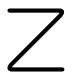
\includegraphics[keepaspectratio]{images/part001_bd86b8f3.jpg}}

换言之，当 I 无界时，若以 \(\mathcal{I}\) 表示由 I 上的规则函数 \(\mathbf{f}\)（取值于 E 且在 I 上有一个积分）所构成的向量空间，则映射 \(\mathbf{f} \mapsto \int_{\mathrm{I}} \mathbf{f}(t) dt\) 在 \(\mathcal{I}\) 赋以 I 上一致收敛的拓扑之后不是连续的（参见 II, p.~53, 推论 2）。

我们将在下列假设之下寻求保证命题 1 成立的充分条件：

\(1^{\circ}\) I 是 \(\mathbf{R}\) 中的任意区间，函数 \(\mathbf{f}_{\alpha}\) 在 I 上是规则的，并且在 I 上有一个积分；

\(2^{\circ}\) 族 \((\mathbf{f}_{\alpha})\) 在含于 I 的每个紧区间上一致收敛于 \(\mathbf{f}\)（关于滤子 \(\mathfrak{F}\)）。

以 \(\mathfrak{K}(\mathrm{I})\) 表示含于 I 的紧区间所成的有向集（II, p.~64），II, p.~68 的公式 (1) 的左端可以写成 \(\lim_{\mathfrak{F}}\left(\lim_{\mathrm{J}\in \mathfrak{K}(\mathrm{I})}\int_{\mathrm{J}}\mathbf{f}_{\alpha}(t)dt\right)\)；
另一方面，考虑到命题 1（II, p.~68）以及族 \((\mathbf{f}_{\alpha})\) 在每个紧区间 \(J \subset I\) 上一致收敛这一事实，(1)（II, p.~68）的右端可以写成 \(\lim_{\mathrm{J} \in \mathfrak{K}(\mathrm{I})} \left( \lim_{\mathfrak{F}} \int_{\mathrm{J}} \mathbf{f}_{\alpha}(t) dt \right)\)。由此看出，只要
对映射 (J, \(\alpha\) ) \(\mapsto \int_{J} f_{\alpha}(t) dt\) 关于滤子 F 以及关于有向集 K(I) 的截口滤子 \(\Phi\) 可以交换极限，II, p.~19 的命题 1 就可以推广。现在，我们知道使这一交换合法的一个充分条件，即映射 (J, \(\alpha\) ) \(\mapsto \int_{J} f_{\alpha}(t) dt\) 关于乘积滤子 \(\Phi \times F\) 的极限存在（Gen.~Top., I, p.~81, 定理 1 的推论）。我们将把这个条件变换为一个等价的、更便于使用的条件。

首先，由于 E 是完备的，为使 \((\mathbf{J}, \alpha) \mapsto \int_{\mathbf{J}} \mathbf{f}_{\alpha}(t) dt\) 关于 \(\Phi \times F\) 有极限，必须且只需：对每个 \(\varepsilon > 0\)，存在一个紧区间 \(J_{0} \subset I\) 和一个集 \(M \in F\)，使得对 M 中任意的元素 \(\alpha\)、\(\beta\) 以及任意的含于 I 的紧区间 \(J \supset J_{0}\)，有

\[
\left\| \int_ {J _ {0}} \mathbf {f} _ {\alpha} (t) d t - \int_ {J} \mathbf {f} _ {\beta} (t) d t \right\| \leqslant \varepsilon .\tag{4}
\]

另一方面我们将证明，这个条件本身等价于下列条件：对每个 \(\varepsilon > 0\)，存在一个紧区间 \(J_0 \subset I\) 和一个集 \(M \in \mathfrak{F}\)，使得对任意的 \(\alpha\)（属于 \(M\)）以及任意的紧区间 \(J \supset J_0\)（含于 \(I\)），有

\[
\left\| \int_ {J _ {0}} \mathbf {f} _ {\alpha} (t) d t - \int_ {J} \mathbf {f} _ {\alpha} (t) d t \right\| \leqslant \varepsilon .\tag{5}
\]

的确，明显可见后一条件是必要的；反之，若它满足，则（由 \((\mathbf{f}_{\alpha})\) 在每个紧区间上的一致收敛性）存在一个集 \(N \in F\)，使得对 N 中任意的 \(\alpha\)、\(\beta\)，有

\[
\left\| \int_ {\mathrm{J} _ {0}} \mathbf {f} _ {\alpha} (t) d t - \int_ {\mathrm{J} _ {0}} \mathbf {f} _ {\beta} (t) d t \right\| \leqslant \varepsilon ;\tag{6}
\]

因而有 \(\left\|\int_{J_{0}}\mathbf{f}_{\alpha}(t)dt-\int_{J}\mathbf{f}_{\beta}(t)dt\right\|\leqslant2\varepsilon\)（对任意的 \(\alpha\) 与 \(\beta\)（属于 \(M\cap N\in\mathfrak{F}\)）以及任意的紧区间 \(J\supset J_{0}\)）。

最后，II, p.~65 的引理使我们能把后一条件写成下列等价形式：对每个 \(\varepsilon > 0\)，存在一个紧区间 \(\mathbf{J}_0 \subset \mathbf{I}\) 和一个集 \(\mathbf{M} \in \mathfrak{F}\)（依赖于 \(\varepsilon\)），使得对每个紧区间 \(\mathbf{K} \subset \mathbf{I}\)（与 \(\mathbf{J}_0\) 无公共内点）以及每个 \(\alpha \in \mathbf{M}\)，有 \(\left\| \int_{\mathbf{K}} \mathbf{f}_{\alpha}(t) dt \right\| \leqslant \varepsilon\)。

最常用的，是一个更强的条件，它是在上述结论中假设集 M 不依赖于 \(\varepsilon\) 而得到的：

定义 1. 我们说积分 \(\int_{\mathrm{I}} \mathbf{f}_{\alpha}(t) dt\) 对 \(\alpha \in \mathrm{A}\) 一致收敛（或在 \(\mathrm{A}\) 上一致收敛），如果对每个 \(\varepsilon > 0\)，存在一个紧区间 \(\mathrm{J}_0 \subset J\)，使得对每个紧区间 \(\mathrm{K} \subset \mathrm{I}\)（与 \(\mathrm{J}_0\) 无公共内点）以及每个 \(\alpha \in \mathrm{A}\)，有

\[
\left\| \int_ {K} \mathbf {f} _ {\alpha} (t) d t \right\| \leqslant \varepsilon .\tag{7}
\]

这个定义等价于说：映射族 \(\alpha\mapsto\int_{J}\mathbf{f}_{\alpha}(t)dt\) 在 A 上一致收敛（收敛于映射 \(\alpha\mapsto\int_{I}\mathbf{f}_{\alpha}(t)dt\)），即关于滤子 \(\Phi\)（\(\Re(I)\) 的截口滤子）而言；诸积分 \(\int_{I}\mathbf{f}_{\alpha}(t)dt\) 中的每一个更是收敛的（反之不真）；此外，由我们刚才所见（或由 Gen.~Top., X, p.~281, 推论 2）：

命题 3. 设 \((\mathbf{f}_{\alpha})\) 是区间 I 上的一个规则函数族，满足：\(1^{\circ}\) 关于滤子 \(\mathfrak{F}\)，族 \((\mathbf{f}_{\alpha})\) 在含于 I 的每个紧区间上一致收敛于一个函数 \(\mathbf{f}\)（在 I 上是规则的）；\(2^{\circ}\) 积分 \(\int_{I} \mathbf{f}_{\alpha}(t) dt\) 对每个 \(\alpha \in A\) 一致收敛。在这些假设之下，积分 \(\int_{I} \mathbf{f}(t) dt\) 收敛，且有

\[
\lim _ {\mathfrak {F}} \int_ {\mathrm{I}} \mathbf {f} _ {\alpha} (t) d t = \int_ {\mathrm{I}} \mathbf {f} (t) d t.\tag{8}
\]

例如当 I 是有界区间、\(\mathbf{f}_{\alpha}\) 在 I 上一致有界且在含于 I 的每个紧区间上一致收敛于 \(\mathbf{f}\) 时，命题 3 的假设满足；事实上，若 \(\| \mathbf{f}_{\alpha}(x)\| \leqslant h\) 对一切 \(x\in \mathrm{I}\) 与一切 \(\alpha\) 成立，且 \(\mathrm{J}_0\) 使得 I 与 \(\mathrm{J}_0\) 的长度之差 \(\leqslant \varepsilon /h\)，则对每个区间 \(\mathrm{K}\subset \mathrm{I}\)（与 \(\mathrm{J}_0\) 无公共内点），条件 (7) 满足。

与 II, p.~68 的命题 1 一样，命题 3 的两个推论在应用中很重要：

推论 1. 设 \((\mathbf{f}_{n})\) 是任意区间 I 上的一个规则函数序列，在含于 I 的每个紧区间上一致收敛于函数 f；若积分 \(\int_{I} \mathbf{f}_{n}(t) dt\) 一致收敛，则积分 \(\int_{I} \mathbf{f}(t) dt\) 收敛，且

\[
\lim _ {n \to \infty} \int_ {\mathrm{I}} \mathbf {f} _ {n} (t) d t = \int_ {\mathrm{I}} \mathbf {f} (t) d t.\tag{9}
\]

注记。这个推论中所加的假设对公式 (9) 的成立是充分的，但不是必要的；以后我们将在推广积分概念的同时推广这个公式（见 INT, IV），并得到弱得多的条件。

推论 2. 设 A 是拓扑空间 F 的一个子集，f 是 I × A 到 R 上的完备赋范空间 E 中的一个映射，使得对每个 \(\alpha \in A\)，函数 \(x \mapsto \mathbf{f}(x, \alpha)\) 在 I 上是规则的。若一方面，函数 \(x \mapsto \mathbf{f}(x, \alpha)\) 在含于 I 的每个紧区间上一致收敛于函数 \(x \mapsto \mathbf{f}(x)\)（当 \(\alpha\) 趋于 \(\alpha_{0} \in \overline{A}\) 而保持属于 A 时）；若另一方面，积分 \(\int_{I} \mathbf{f}(x, \alpha) dx\) 在 A 上一致收敛，则积分 \(\int_{I} \mathbf{f}(x) dx\) 收敛，且有

\[
\lim _ {\alpha \rightarrow \alpha_ {0}, \alpha \in A} \int_ {I} \mathbf {f} (x, \alpha) d x = \int_ {I} \mathbf {f} (x) d x.\tag{10}
\]

特别地：

命题 4（“反常积分对参数的连续性”）。设 F 是紧空间，I 是 R 中的任意区间，f 是 I × F 到 R 上的完备赋范空间 E 中的连续映射；若积分 \(\mathbf{h}(\alpha) = \int_{\mathrm{I}} \mathbf{f}(x, \alpha) dx\) 在 F 上一致收敛，则它是 \(\alpha\) 在 F 上的连续函数。

由于 II, p.~69 的命题 2，本命题也可由连续函数的一致极限的连续性（Gen.~Top., X, p.~282, 定理 2）得出。

\subsection{正规收敛积分}

设 \((\mathbf{f}_{\alpha})_{\alpha\in\mathrm{A}}\) 是任意区间 \(I\subset R\) 上的一个规则函数族，取值于 R 上的完备赋范空间 E 中。假设存在 I 上的一个有限实规则函数 g，使得对每个 \(x\in I\) 与每个 \(\alpha\in A\)，\(\|f_{\alpha}(x)\|\leqslant g(x)\)，并且积分 \(\int_{I}g(t)dt\) 收敛。在这些条件之下，积分 \(\int_{I}\mathbf{f}_{\alpha}(t)dt\) 在 A 上绝对且一致收敛；事实上，对含于 I 的每个紧区间 K，

\[
\left\| \int_ {K} \mathbf {f} _ {\alpha} (t) d t \right\| \leqslant \int_ {K} g (t) d t
\]

而积分 \(\int_{I} g(t) dt\) 的收敛性蕴含：对每个 \(\varepsilon > 0\)，存在一个紧区间 \(J \subset I\)，使得对每个与 J 不相交的紧区间 \(K \subset I\)，有 \(\int_{K} g(t) dt \leqslant \varepsilon\)。当存在一个具有上述性质的实函数 g 时，我们就说积分 \(\int_{I} f_{\alpha}(t) dt\) 在 A 上正规收敛（参见 Gen.~Top., X, p.~296）。

一个积分可以在 A 上一致收敛而非正规收敛。*实函数序列 \((f_n)\) 由下列条件定义：\(f_n(x) = 1 / x\)（当 \(n \leqslant x \leqslant n + 1\)），\(f_n(x) = 0\)（当 \(x\) 在 \(\mathbf{I} = [\mathbf{0}, +\infty[\) 中取其他值），对它就出现这种情形。立即可以看出，积分 \(\int_{1}^{\infty} f_n(t) dt\) 一致收敛，但非正规收敛，因为关系式 \(g(x) \geqslant f_n(x)\)（对每个 \(x \in \mathbf{I}\) 与所有 \(n\)）蕴含 \(g(x) \geqslant 1 / x\)，从而 \(g\) 在 \(\mathbf{I}\) 上的积分不收敛。*

特别地，考虑一个级数，其通项 \(u_{n}\) 是区间 I 上的规则函数，并假设以 \(\|u_{n}(x)\|\)（它是 I 上的规则函数）为通项的级数在含于 I 的每个紧区间上一致收敛，且以 \(\int_{I}\|\mathbf{u}_{n}(t)\|dt\) 为通项的级数收敛；于是（II, p.~66, 命题 2）（规则的）函数 \(g(x)\)——即以 \(\|u_{n}(x)\|\) 为通项的级数之和——使得积分 \(\int_{I}g(t)dt\) 收敛。若令 \(f_{n}=\sum_{p=1}^{n}u_{p}\)，则积分 \(\int_{I}f_{n}(t)dt\) 正规收敛，因为有

\[
\left\| \mathbf {f} _ {n} (x) \right\| \leqslant \sum_ {p = 1} ^ {n} \left\| \mathbf {u} _ {p} (x) \right\| \leqslant g (x)
\]

对一切 \(x \in \mathrm{I}\) 与一切 \(n\) 成立；因此，和 \(\mathbf{f}\)——即以 \(\mathbf{u}_n\) 为通项的级数之和——是 \(\mathrm{I}\) 上的规则函数，且积分 \(\int_{\mathrm{I}} \mathbf{f}(t) dt\) 收敛，并有

\[
\int_ {\mathrm{I}} \mathbf {f} (t) d t = \sum_ {n = 1} ^ {\infty} \int_ {\mathrm{I}} \mathbf {u} _ {n} (t) d t\tag{11}
\]

（“非紧区间上级数的逐项积分”）。

\subsection{紧区间上积分对参数的导数}

设 A 是域 R（相应地，域 C）中一点 \(\alpha_{0}\) 的紧邻域，I = {[}a, b{]} 是 R 中的紧区间，f 是 I × A 到 R（相应地，C）上的完备赋范空间 E 中的连续映射。我们已经看到（II, p.~69, 命题 2），在这些条件之下 \(\mathbf{g}(\alpha) = \int_{a}^{b} \mathbf{f}(t, \alpha) dt\) 是 A 上的连续函数。我们来寻求使 g 在点 \(\alpha_{0}\) 处有导数的充分条件。对 \(\alpha \neq \alpha_{0}\)，有

\[
\frac {\mathbf {g} (\alpha) - \mathbf {g} (\alpha_ {0})}{\alpha - \alpha_ {0}} = \int_ {a} ^ {b} \frac {\mathbf {f} (t , \alpha) - \mathbf {f} (t , \alpha_ {0})}{\alpha - \alpha_ {0}} d t
\]

因而（II, p.~69, 推论 2），若函数 \(x \mapsto \frac{\mathbf{f}(x, \alpha) - \mathbf{f}(x, \alpha_0)}{\alpha - \alpha_0}\) 在 I 上一致收敛于一个（必然连续的）函数 \(x \mapsto \mathbf{h}(x)\)（当 \(\alpha\) 趋于 \(\alpha_0\) 而保持 \(\neq \alpha_0\) 时），则 \(\mathbf{g}\) 有一个等于 \(\int_{a}^{b} \mathbf{h}(t) dt\) 的导数（在点 \(\alpha_0\) 处）；此外，对每个 \(x \in I\)，\(\frac{\mathbf{f}(x, \alpha) - \mathbf{f}(x, \alpha_0)}{\alpha - \alpha_0}\) 趋于 \(\mathbf{h}(x)\)，故 \(\mathbf{h}(x)\) 是在点 \(\alpha_0\) 处映射 \(\alpha \mapsto \mathbf{f}(x, \alpha)\) 的导数；我们把这个导数（称为 \(\mathbf{f}\) 关于 \(\alpha\) 的偏导数）记作 \(\mathbf{f}_{\alpha}'(x, \alpha_0)\)；我们所做的假设蕴含

\[
\mathbf {g} ^ {\prime} (\alpha_ {0}) = \int_ {a} ^ {b} \mathbf {f} _ {\alpha} ^ {\prime} (t, \alpha_ {0}) d t.\tag{12}
\]

下面的命题给出使公式 (12) 成立的一个非常简单的充分条件：

命题 5. 假设偏导数 \(\mathbf{f}_{\alpha}^{\prime}(x,\alpha)\) 对所有 \(x\in \mathrm{I}\) 与所有 \(\alpha\)（属于 \(\mathbf{V}\)，即 \(\alpha_0\) 的一个开邻域）存在，并且对所有 \(\alpha \in \mathbf{V}\)，映射 \(x\mapsto \mathbf{f}_{\alpha}^{\prime}(x,\alpha)\) 在 \(\mathrm{I}\) 上是规则的。在这些条件之下，若 \(x\mapsto \mathbf{f}_{\alpha}^{\prime}(x,\alpha)\) 在 \(\mathrm{I}\) 上一致收敛于 \(x\mapsto \mathbf{f}_{\alpha}^{\prime}(x,\alpha_0)\)（当 \(\alpha\) 趋于 \(\alpha_0\) 时），则函数 \(\mathbf{g}(\alpha) = \int_{a}^{b}\mathbf{f}(t,\alpha)dt\) 有一个由公式 (12) 给出的导数（在点 \(\alpha_0\) 处）。

事实上，对每个 \(\varepsilon > 0\)，由假设存在一个 \(r > 0\)，使得 \(|\alpha - \alpha_0| \leqslant r\) 蕴含 \(\left\| \mathbf{f}_{\alpha}'(x, \alpha) - \mathbf{f}_{\alpha}'(x, \alpha_0) \right\| \leqslant \varepsilon\)（对任何 \(x \in I\)）。由 I, p.~17 的命题 3 与命题 5，对 \(|\alpha - \alpha_0| \leqslant r\)（\(\alpha \neq \alpha_0\)）与所有 \(x \in I\)，有

\[
\left| \left| \frac {\mathbf {f} (x , \alpha) - \mathbf {f} (x , \alpha_ {0})}{\alpha - \alpha_ {0}} - \mathbf {f} _ {\alpha} ^ {\prime} (x, \alpha_ {0}) \right| \right| \leqslant \varepsilon
\]

这就证明了 \(\frac{\mathbf{f}(x,\alpha)-\mathbf{f}(x,\alpha_{0})}{\alpha-\alpha_{0}}\) 一致收敛于 \(\mathbf{f}_{\alpha}^{\prime}(x,\alpha_{0})\)（在 I 上，当 \(\alpha\) 趋于 \(\alpha_{0}\) 且保持 \(\neq\alpha_{0}\) 时），从而建立了公式 (12)。

推论。若偏导数 \(\mathbf{f}_{\alpha}^{\prime}(x,\alpha)\) 在 I × V 上存在且是 \((x,\alpha)\) 在这个集合上的连续函数，则函数 g 在点 \(\alpha_{0}\) 处有一个由公式 (12) 给出的导数。

事实上，若 W 是含于 V 的 \(\alpha_{0}\) 的紧邻域，则映射 \((x,\alpha)\mapsto\mathbf{f}_{\alpha}^{\prime}(x,\alpha)\) 在紧集 I × W 上一致连续，故 \(\mathbf{f}_{\alpha}^{\prime}(x,\alpha)\) 一致收敛于 \(\mathbf{f}_{\alpha}^{\prime}(x,\alpha_{0})\)（在 I 上，当 \(\alpha\) 趋于 \(\alpha_{0}\) 时）。

由命题 5 可以推出一个更一般的命题，它使我们在被积函数 f 以及积分限都依赖于一个参数 \(\alpha\) 时也能求出积分的导数：

命题 6. 在命题 5 的假设满足之下，设 \(a(\alpha)\)、\(b(\alpha)\) 是定义在 V 上、取值于 I 中的两个函数；若导数 \(a'(\alpha_0)\)、\(b'(\alpha_0)\) 存在且有限，则函数 \(\mathbf{g}(\alpha) = \int_{a(\alpha)}^{b(\alpha)} \mathbf{f}(t, \alpha) dt\) 在 \(\alpha_0\) 处有一个由下式给出的导数

\[
\mathbf {g} ^ {\prime} (\alpha_ {0}) = \int_ {a (\alpha_ {0})} ^ {b (\alpha_ {0})} \mathbf {f} _ {\alpha} ^ {\prime} (t, \alpha_ {0}) d t + b ^ {\prime} (\alpha_ {0}) \mathbf {f} (b (\alpha_ {0}), \alpha_ {0}) - a ^ {\prime} (\alpha_ {0}) \mathbf {f} (a (\alpha_ {0}), \alpha_ {0}).\tag{13}
\]

事实上，对所有 \(\alpha \in \mathbf{V}\)（异于 \(\alpha_0\)），可以写出

\[
\begin{array}{c} \frac {\mathbf {g} (\alpha) - \mathbf {g} (\alpha_ {0})}{\alpha - \alpha_ {0}} = \int_ {a (\alpha_ {0})} ^ {b (\alpha_ {0})} \frac {\mathbf {f} (t , \alpha) - \mathbf {f} (t , \alpha_ {0})}{\alpha - \alpha_ {0}} d t + \frac {1}{\alpha - \alpha_ {0}} \int_ {b (\alpha_ {0})} ^ {b (\alpha)} \mathbf {f} (t, \alpha) d t \\ - \frac {1}{\alpha - \alpha_ {0}} \int_ {a (\alpha_ {0})} ^ {a (\alpha)} \mathbf {f} (t, \alpha) d t. \end{array}
\]

由 II, p.~74 的命题 5，右端的第一个积分趋于 \(\int_{a(\alpha_0)}^{b(\alpha_0)} \mathbf{f}'_\alpha(t, \alpha_0) dt\)（当 \(\alpha\) 趋于 \(\alpha_0\) 时）。在第二个积分中，我们把 \(\mathbf{f}(t, \alpha)\) 换成 \(\mathbf{f}(b(\alpha_0), \alpha_0)\)，并证明其差趋于 0。令 \(\mathbf{M} = \operatorname{Max}\big( \| \mathbf{f}(b(\alpha_0), \alpha_0) \|, |b'(\alpha_0)| + 1 \big)\)；由于函数 \(b(\alpha)\) 在点 \(\alpha_0\) 连续，函数 \(\mathbf{f}\) 在点 \((b(\alpha_0), \alpha_0)\) 连续，故对每个 \(\varepsilon\)（满足 \(0 < \varepsilon < 1\)）存在一个 \(r > 0\)，使得关系 \(|\alpha - \alpha_0| \leqslant r\) 蕴含 \(\| \mathbf{f}(t, \alpha) - \mathbf{f}(b(\alpha_0), \alpha_0) \| \leqslant \varepsilon\)（对所有 \(t\)，它属于以 \(b(\alpha_0)\) 与 \(b(\alpha)\) 为端点的区间）；于是还可以假设关系 \(|\alpha - \alpha_0| \leqslant r\) 蕴含 \(\left| \frac{b(\alpha) - b(\alpha_0)}{\alpha - \alpha_0} - b'(\alpha_0) \right| \leqslant \varepsilon\)。

于是，由中值公式（II, p.~62, 公式 (17)）有

\[
\left\| \frac {1}{\alpha - \alpha_ {0}} \int_ {b (\alpha_ {0})} ^ {b (\alpha)} \mathbf {f} (t, \alpha) d t - \frac {b (\alpha) - b (\alpha_ {0})}{\alpha - \alpha_ {0}} \mathbf {f} (b (\alpha_ {0}), \alpha_ {0}) \right\| \leqslant \left| \frac {b (\alpha) - b (\alpha_ {0})}{\alpha - \alpha_ {0}} \right| \varepsilon
\]

从而

\[
\left\| \frac {1}{\alpha - \alpha_ {0}} \int_ {b (\alpha_ {0})} ^ {b (\alpha)} \mathbf {f} (t, \alpha) d t - b ^ {\prime} (\alpha_ {0}) \mathbf {f} (b (\alpha_ {0}), \alpha_ {0}) \right\| \leqslant 2 \mathrm{M} \varepsilon
\]

这表明 \(\frac{1}{\alpha - \alpha_0} \int_{b(\alpha_0)}^{b(\alpha)} \mathbf{f}(t, \alpha) dt\) 趋于 \(b'(\alpha_0)\mathbf{f}(b(\alpha_0), \alpha_0)\)。同理可证 \(\frac{1}{\alpha - \alpha_0} \int_{a(\alpha_0)}^{a(\alpha)} \mathbf{f}(t, \alpha) dt\) 趋于 \(a'(\alpha_0)\mathbf{f}(a(\alpha_0), \alpha_0)\)。

\subsection{非紧区间上积分对参数的导数}

设集 V 与 II, p.~74 的命题 5 中的含义相同，现在假设 I 是 R 中的任意区间，f 是 I × V 到 E 中的连续映射；若积分 \(\mathbf{g}(\alpha) = \int_{\mathrm{I}} \mathbf{f}(t, \alpha) dt\) 对所有 \(\alpha \in V\) 存在且是 \(\alpha\) 的连续函数，则函数 g 未必有一个等于 \(\int_{\mathrm{I}} \mathbf{f}'_{\alpha}(t, \alpha_0) dt\) 的导数（在点 \(\alpha_0\) 处），即使 \(\mathbf{f}'_{\alpha}(x, \alpha)\)

在含于 I 的每个紧区间上一致收敛于 \(\mathbf{f}_{\alpha}^{\prime}(x,\alpha_{0})\)，且积分 \(\int_{\mathrm{I}}\mathbf{f}_{\alpha}^{\prime}(t,\alpha)dt\) 对所有 \(\alpha \in \mathrm{V}\) 存在（参见 II, p.~87, 习题 3）。

下面的命题给出了使公式 (12)（II, p.~74）仍然成立的一个充分条件：

命题 7. 设 I 是 \(\mathbf{R}\) 中的任意区间，\(\mathbf{f}\) 是 \(\mathrm{I} \times \mathrm{V}\) 上的连续函数。假设：

\(1^{\circ}\) 偏导数 \(\mathbf{f}_{\alpha}^{\prime}(x,\alpha)\) 对所有 \(x\in \mathrm{I}\) 与所有 \(\alpha \in \mathrm{V}\) 存在，且对所有 \(\alpha \in \mathrm{V}\)，映射 \(x\mapsto \mathbf{f}_{\alpha}^{\prime}(x,\alpha)\) 在 \(\mathrm{I}\) 上是规则的；

\(2^{\circ}\) 对所有 \(\alpha \in \mathrm{V}\)，\(\mathbf{f}_{\alpha}^{\prime}(x,\beta)\) 一致收敛于 \(\mathbf{f}_{\alpha}^{\prime}(x,\alpha)\)（在含于 I 的每个紧区间上，当 \(\beta\) 趋于 \(\alpha\) 时）；

\(3^{\circ}\) 积分 \(\int_{\mathrm{I}}\mathbf{f}_{\alpha}^{\prime}(t,\alpha)dt\) 在 \(\mathrm{V}\) 上一致收敛；

\(4^{\circ}\) 积分 \(\int_{\mathrm{I}}\mathbf{f}(t,\alpha_0)dt\) 收敛。

在这些条件之下，积分 \(\mathbf{g}(\alpha)=\int_{\mathrm{I}}\mathbf{f}(t,\alpha)dt\) 在 V 上一致收敛，且函数 g 在 V 的每一点处有一个由下式给出的导数

\[
\mathbf {g} ^ {\prime} (\alpha) = \int_ {\mathrm{I}} \mathbf {f} _ {\alpha} ^ {\prime} (t, \alpha) d t.\tag{14}
\]

\(\int_{\mathrm{I}} \mathbf{f}_{\alpha}'(t, \alpha) dt\) 在 V 上的一致收敛意味着：函数 \(\alpha \mapsto \int_{\mathrm{J}} \mathbf{f}_{\alpha}'(t, \alpha) dt\) 在 V 上关于滤子 \(\Phi\)——即有向集 \(\Re(\mathrm{I})\)（由含于 I 的紧区间 J 组成）的截口滤子——一致收敛。令 \(\mathbf{u}_{\mathrm{J}}(\alpha) = \int_{\mathrm{J}} \mathbf{f}(t, \alpha) dt\)；这些假设表明，一方面 \(\mathbf{u}_{\mathrm{J}}(\alpha_0)\) 关于 \(\Phi\) 有一个极限，另一方面，由 II, p.~74 的命题 5，有 \(\mathbf{u}_{\mathrm{J}}'(\alpha) = \int_{\mathrm{J}} \mathbf{f}_{\alpha}'(t, \alpha) dt\)（对一切 \(\alpha \in \mathrm{V}\)）。因此我们可以把 II, p.~52 的定理 1 应用于函数 \(\mathbf{u}_{\mathrm{J}}\)，这里指标集的角色由 \(\Re(\mathrm{I})\) 扮演，而这个集合上的滤子的角色由滤子 \(\Phi\) 扮演；命题随之立得。

注记。1) 命题 7 的条件 \(1^{\circ}\) 与 \(2^{\circ}\) 更是满足的，当 \(\mathbf{f}_{\alpha}^{\prime}(x,\alpha)\) 是 \((x,\alpha)\) 在 \(\mathrm{I} \times \mathrm{V}\) 上的连续函数时。

\begin{enumerate}
\def\labelenumi{\arabic{enumi})}
\setcounter{enumi}{1}
\tightlist
\item
  在积分 \(\int_{a(\alpha)}^{b(\alpha)}\mathbf{f}(t,\alpha)dt\) 中，当区间的端点是参数的有限函数时，把这个积分作为 \(\alpha\) 的函数来研究可以化为对 {[}0, 1{]} 上积分的研究；事实上，通过变量替换 \(t = a(\alpha)(1 - u) + b(\alpha)u\)，有
\end{enumerate}

\[
\int_ {a (\alpha)} ^ {b (\alpha)} \mathbf {f} (t, \alpha) d t = \int_ {0} ^ {1} \mathbf {f} (a (\alpha) (1 - u) + b (\alpha) u, \alpha) (b (\alpha) - a (\alpha)) d u.
\]

\subsection{积分次序的交换}

设 \(I = [a, b]\) 与 \(A = [c, d]\) 是 \(R\) 中的两个紧区间；设 \(f\) 是 \(I \times A\) 上的连续函数，取值于完备赋范空间 \(E\)（定义在 \(R\) 上）中；由 II, p.~69 的命题 2，\(\int_{a}^{b} f(x, \alpha) dx\) 是 \(\alpha\) 在 \(A\) 上的连续函数；为简单起见，它的积分 \(\int_{c}^{d} \left( \int_{a}^{b} f(x, \alpha) dx \right) d\alpha\) 也记作 \(\int_{c}^{d} d\alpha \int_{a}^{b} f(x, \alpha) dx\)。

命题 8. 若 \(\mathbf{f}\) 在 \(\mathrm{I} \times \mathrm{A}\) 上连续，则有

\[
\int_ {c} ^ {d} d \alpha \int_ {a} ^ {b} \mathbf {f} (x, \alpha) d x = \int_ {a} ^ {b} d x \int_ {c} ^ {d} \mathbf {f} (x, \alpha) d \alpha\tag{15}
\]

（“交换积分次序的公式”）。

我们将证明，对所有 \(y \in A\)，有

\[
\int_ {c} ^ {y} d \alpha \int_ {a} ^ {b} \mathbf {f} (x, \alpha) d x = \int_ {a} ^ {b} d x \int_ {c} ^ {y} \mathbf {f} (x, \alpha) d \alpha .\tag{16}
\]

由于 (16) 的两端都是 \(y\) 的函数，且在 \(y = c\) 时相等，故只需证明它们在 \(]c\) , \(d[\) 上可微且其导数在这个区间的每一点处相等。若令 \(\mathbf{g}(\alpha) = \int_{a}^{b} \mathbf{f}(x, \alpha) dx\) 与 \(\mathbf{h}(x, y) = \int_{c}^{y} \mathbf{f}(x, \alpha) dx\)，则关系式 (16) 可以写成

\[
\int_ {c} ^ {y} \mathbf {g} (\alpha) d \alpha = \int_ {a} ^ {b} \mathbf {h} (x, y) d x.
\]

而第一项对 \(y\) 的导数是 \(\mathbf{g}(y)\)，第二项的导数是 \(\int_{a}^{b} \mathbf{h}_{y}'(x, y) dx\)（由 II, p.74, 推论），因为 \(\mathbf{h}_{y}'(x, y) = \mathbf{f}(x, y)\) 在 \(I \times A\) 上连续；这样得到的两个表达式是相同的。

现在设 A = {[}c, d{]} 是 R 中的紧区间，I 是 R 中的任意区间；设 f 是 I × A 上的连续函数，取值于 E 中，使得积分 \(\mathbf{g}(\alpha) = \int_{\mathrm{I}} \mathbf{f}(t, \alpha) dt\) 对所有 \(\alpha \in A\) 收敛；即使 \(\mathbf{g}(\alpha)\) 在 A 上连续，也未必总能在积分 \(\int_{c}^{d} d\alpha \int_{I} \mathbf{f}(t, \alpha) dt\) 中交换积分次序，因为积分 \(\int_{I} dt \int_{c}^{d} \mathbf{f}(t, \alpha) d\alpha\) 可能不存在，或者可能与积分 \(\int_{c}^{d} d\alpha \int_{I} \mathbf{f}(t, \alpha) dt\) 不同（参见 II, p.~87, 习题 7）。然而有下列结果：

命题 9. 若函数 \(\mathbf{f}\) 在 \(\mathrm{I} \times \mathrm{A}\) 上连续，且积分 \(\int_{\mathrm{I}} \mathbf{f}(t, \alpha) dt\) 在 \(\mathrm{A}\) 上一致收敛，则积分 \(\int_{\mathrm{I}} dt \int_{c}^{d} \mathbf{f}(t, \alpha) d\alpha\) 收敛，且有

\[
\int_ {c} ^ {d} d \alpha \int_ {\mathrm{I}} \mathbf {f} (t, \alpha) d t = \int_ {\mathrm{I}} d t \int_ {c} ^ {d} \mathbf {f} (t, \alpha) d \alpha .\tag{17}
\]

对含于 I 的每个紧区间 J，令 \(\mathbf{u}_{\mathrm{J}}(\alpha) = \int_{\mathrm{J}} \mathbf{f}(t, \alpha) dt\)。这个假设蕴含：关于滤子 \(\Phi\)（有向集 \(\Re(\mathrm{I})\) 的截口滤子），连续函数 \(u_{J}\) 在 A 上一致收敛于 \(\int_{I} f(t, \alpha) dt\)；于是（II, p.~68, 命题 1），\(\int_{c}^{d} d\alpha \int_{J} f(t, \alpha) dt\) 有极限 \(\int_{c}^{d} d\alpha \int_{I} f(t, \alpha) dt\)（关于 \(\Phi\)）；但由命题 8（II, p.~77），有

\[
\int_ {c} ^ {d} d \alpha \int_ {\mathrm{J}} \mathbf {f} (t, \alpha) d t = \int_ {\mathrm{J}} d t \int_ {c} ^ {d} \mathbf {f} (t, \alpha) d \alpha .\tag{18}
\]

前面的结果于是表明积分 \(\int_{I} dt \int_{c}^{d} \mathbf{f}(t, \alpha) d\alpha\) 收敛，而且在关系式 (18) 中关于 \(\Phi\) 取极限，便得到 (17)。

\setcounter{exercisegroup}{0}
\refstepcounter{exercisegroup}
\section*{第 \S\arabic{exercisegroup} 节习题}
\phantomsection
\addcontentsline{toc}{section}{第 \protect\S\arabic{exercisegroup} 节习题}

\begin{enumerate}
\def\labelenumi{\arabic{enumi})}
\tightlist
\item
  设 \((f_{\alpha})\) 是一族实函数，定义在区间 \(\mathrm{I} \subset \mathbf{R}\) 上，其中每个函数在 \(\mathrm{I}\) 上有一个严格原函数，并且它们关于关系 \(\leqslant\) 构成一个有向集。设 \(f\) 是族 \((f_{\alpha})\) 的上包络；假设 \(f\) 在 \(\mathrm{I}\) 上有一个严格原函数。证明：若 \(g_{\alpha}\)（相应地，\(g\)）是 \(f_{\alpha}\)（相应地，\(f\)）的在点 \(x_0 \in \mathrm{I}\) 处为零的原函数，则 \(g\) 是族 \((g_{\alpha})\) 在交集 \(\mathrm{I} \cap [x_0, +\infty[\) 上的上包络，而是它在交集 \(\mathrm{I} \cap ] - \infty\) , \(x_0]\) 上的下包络。（限于这两个区间中的第一个，证明：若 \(u\) 是 \((g_{\alpha})\) 在 \(\mathrm{I} \cap [x_0, +\infty[\) 上的上包络，则 \(u(x + h) - u(x) \leqslant g(x + h) - g(x)\)（对 \(h > 0\)）成立；然后证明，对一切 \(\alpha\)，有 \(u(x + h) - u(x) \geqslant g_{\alpha}(x + h) - g_{\alpha}(x)\)，并由最后这个不等式断定 \(\liminf_{h \to 0} (u(x + h) - u(x))/h \geqslant f(x)\)；由此推出命题。）
\end{enumerate}

给出一个区间 I 上的递增连续函数序列 \((f_n)\) 的例子，这些函数一致有界，但其上包络在 I 上没有严格原函数。

\begin{enumerate}
\def\labelenumi{\arabic{enumi})}
\setcounter{enumi}{1}
\item
  证明：为使函数 \(\mathbf{f}\) 是区间 I 上的阶梯函数，必须且只需它只有有限个不连续点，并且在它连续的每个区间上取常值。
\item
  设 \(\mathbf{f}\) 是区间 \(I \subset \mathbf{R}\) 上的规则函数，取值于完备赋范空间 \(E\)（\(\mathbf{R}\) 上的）中；证明：对每个紧子集 \(H\)（含于 \(I\)），集合 \(\mathbf{f}(H)\) 在 \(E\) 中是相对紧的；给出一个 \(\mathbf{f}(H)\) 在 \(E\) 中不是闭集的例子。
\item
  给出一个连续实函数 \(f\)（在紧区间 \(\mathrm{I} \subset \mathbf{R}\) 上）的例子，使得复合函数 \(x \mapsto \operatorname{sgn}(f(x))\) 在 \(\mathrm{I}\) 上不是规则的（尽管 \(\operatorname{sgn}\) 在 \(\mathbf{R}\) 上是规则的）。
\item
  设 \(\mathbf{f}\) 是定义在紧区间 \(\mathrm{I} = [a, b] \subset \mathbf{R}\) 上、取值于完备赋范空间 \(\mathrm{E}\) 中的向量函数；我们说 \(\mathbf{f}\) 在 \(\mathrm{I}\) 上是有界变差的，如果存在一个数 \(m > 0\)，使得对每个有限的严格递增序列 \((x_i)_{0 \leqslant i \leqslant n}\)——由
\end{enumerate}

I 中满足 \(x_0 = a\) 与 \(x_n = b\) 的点组成——有 \(\sum_{i=0}^{n-1} \| \mathbf{f}(x_{i+1}) - \mathbf{f}(x_i) \| \leqslant m\)。

\begin{enumerate}
\def\labelenumi{\alph{enumi})}
\item
  证明 \(\mathbf{f}(\mathrm{I})\) 在 E 中相对紧（用反证法论证）。
\item
  证明 \(\mathbf{f}\) 在 I 上是规则的（证明当 \(x\) 趋于一点 \(x_0 \in \mathrm{I}\) 而保持 \(>x_0\) 时，函数 \(\mathbf{f}\) 不可能有两个不同的聚点，并利用 \(a\)））。
\end{enumerate}

\begin{enumerate}
\def\labelenumi{\arabic{enumi})}
\setcounter{enumi}{5}
\tightlist
\item
  为使函数 \(\mathbf{f}\)（取值于完备赋范空间 \(E\) 中、定义在开区间 \(I \subset R\) 上）在 \(I\) 的一个可数子集的余集的所有点处等于 \(I\) 上的一个规则函数，必须且只需它满足下列条件：对每个 \(x \in I\) 与每个 \(\varepsilon > 0\)，存在一个数 \(h > 0\) 和两个元素 \(a\)、\(b\)（\(E\) 的），使得 \(\| \mathbf{f}(y) - a \| \leqslant \varepsilon\) 对每个 \(y \in [x, x + h]\) 都成立（至多除去这个区间的可数无穷多个点），且 \(\| \mathbf{f}(z) - b \| \leqslant \varepsilon\) 对所有 \(z \in [x - h, x]\) 成立（至多除去这个区间的可数无穷多个点）。
\end{enumerate}

* 7) 证明：等于 \(\sin(1/x)\)（当 \(x \neq 0\)）而等于 0（当 \(x = 0\)）的函数在 \(\mathbf{R}\) 上有一个严格原函数（注意 \(x^2 \sin(1/x)\) 在每一点处有导数）。

由此推出：若 \(g(x,u,v)\) 是 u, v 的多项式，其系数是 x 在区间 I（包含 0）上的连续函数，则等于 \(g(x,\sin1/x,\cos1/x)\)（当 \(x\neq0\)）而等于一个适当的值 \(\alpha\)（待定）（当 x=0）的函数在 I 上有一个严格原函数；给出一个 \(\alpha\neq g(0,0,0)\) 的例子。

* 8) 证明：存在 \([-1, +1]\) 上的连续函数，在这个区间的每一点处有有限导数，这个导数等于 \(\sin\left(\frac{1}{\sin 1/x}\right)\)（在每一点 \(x\) 处，只要 x 异于 \(1/n\pi\)（\(n\) 为整数 \(\neq 0\)）且异于 0）。（在 \(x = 1/n\pi\) 的邻域内作变量替换 \(x = \frac{1}{n\pi + \operatorname{Arc} \sin u}\) 并利用习题 7；借助同样的变量替换证明，存在一个常数 \(a > 0\)（与 \(n\) 无关），使得

\[
\left| \int_ {2 / (2 n + 1) \pi} ^ {2 / (2 n - 1) \pi} \sin \left(\frac {1}{\sin \frac {1}{x}}\right) d x \right| \leqslant \frac {a}{n ^ {3}};
\]

并由此断定，若令

\[
g (x) = \lim _ {\varepsilon \rightarrow 0} \int_ {\varepsilon} ^ {x} \sin \left(\frac {1}{\sin \frac {1}{t}}\right) d t,
\]

则 g 在点 x = 0 处有一个等于 0 的导数。）*

\begin{enumerate}
\def\labelenumi{\arabic{enumi})}
\setcounter{enumi}{8}
\item
  设 \(\mathbf{f}\) 是紧区间 \(\mathrm{I} = [a, b]\) 上的规则函数。证明：对每个 \(\varepsilon > 0\)，存在一个连续函数 \(\mathbf{g}\)（在 \(\mathrm{I}\) 上），使得 \(\int_{a}^{b} \| \mathbf{f}(t) - \mathbf{g}(t) \| dt \leqslant \varepsilon\)（化为 \(\mathbf{f}\) 是阶梯函数的情形）。由此推出存在一个多项式 \(\mathbf{h}\)（系数在 E 中），使得 \(\int_{a}^{b} \| \mathbf{f}(t) - \mathbf{h}(t) \| dt \leqslant \varepsilon\)。
\item
  设 \(\mathbf{f}\) 是 \([a, b]\) 上的规则函数，取值于 E 中；设 \(\mathbf{g}\) 是 \([a, c]\)（\(c > b\)）上的规则函数，取值于 F 中；并设 \((\mathbf{x}, \mathbf{y}) \mapsto [\mathbf{x}, \mathbf{y}]\) 是 \(\mathrm{E} \times \mathrm{F}\) 到 G 中的连续双线性映射（E, F, G 是完备赋范空间）。证明
\end{enumerate}

\[
\lim _ {h \rightarrow 0, h > 0} \int_ {a} ^ {b} [ \mathbf {f} (t). \mathbf {g} (t + h) ] d t = \int_ {a} ^ {b} [ \mathbf {f} (t). \mathbf {g} (t) ] d t
\]

（化为 \(\mathbf{f}\) 是阶梯函数的情形）。

\begin{enumerate}
\def\labelenumi{\arabic{enumi})}
\setcounter{enumi}{10}
\tightlist
\item
  在与习题 10 相同的假设下，证明：对每个 \(\varepsilon > 0\)，存在一个数 \(\rho > 0\)，使得把 \([a, b]\) 分成区间 \([x_i, x_{i+1}]\)（长度 \(\leqslant \rho\)，\(0 \leqslant i \leqslant n-1\)）的每个分割，有
\end{enumerate}

\[
\left\| \int_ {a} ^ {b} [ \mathbf {f} (t). \mathbf {g} (t) ] d t - \sum_ {i = 0} ^ {n - 1} [ \mathbf {f} (u _ {i}). \mathbf {g} (v _ {i}) ] (x _ {i + 1} - x _ {i}) \right\| \leqslant \varepsilon
\]

对每个指标 i，不论点 \(u_{i}\)、\(v_{i}\)（取自 \([x_{i}, x_{i+1}]\)）如何选取（化为 f 与 g 都是阶梯函数的情形）。

¶ 12) 我们说实数序列 \((x_{n})\)（含于区间 \([0, 1]\)）在这个区间中是一致分布的，如果

\[
\lim _ {n \to \infty} \frac {\nu_ {n} (\alpha , \beta)}{n} = \beta - \alpha\tag{1}
\]

对每对数 \(\alpha\)、\(\beta\)（满足 \(0 \leqslant \alpha \leqslant \beta \leqslant 1\)）都成立，其中 \(\nu_{n}(\alpha, \beta)\) 表示指标 \(i\)（满足 \(1 \leqslant i \leqslant n\) 且 \(\alpha \leqslant x_{i} \leqslant \beta\)）的个数。

证明：若序列 \((x_{n})\) 一致分布且 \(\mathbf{f}\) 是 \([0, 1]\) 上的规则函数，则

\[
\lim _ {n \rightarrow \infty} \frac {1}{n} \sum_ {i = 1} ^ {n} \mathbf {f} (x _ {i}) = \int_ {0} ^ {1} \mathbf {f} (t) d t\tag{2}
\]

（化为 \(\mathbf{f}\) 是阶梯函数的情形）。逆命题。

证明：为使序列 \((x_{n})\) 一致分布，只需关系 (2) 对每个实函数 f（属于赋以一致收敛拓扑的 {[}0, 1{]} 上实连续函数空间中的一个稠密集）成立。

¶ 13) 设 \(f\) 是紧区间 \([a, b]\) 上的实规则函数。令

\[
r (n) = \frac {b - a}{n} \sum_ {k = 1} ^ {n} f \left(a + k \frac {b - a}{n}\right) - \int_ {a} ^ {b} f (t) d t.
\]

\begin{enumerate}
\def\labelenumi{\alph{enumi})}
\tightlist
\item
  证明：若 \(f\) 在 \([a, b]\) 上递增，则
\end{enumerate}

\[
0 \leqslant r (n) \leqslant \frac {b - a}{n} \Bigl (f (b) - f (a) \Bigr).
\]

\begin{enumerate}
\def\labelenumi{\alph{enumi})}
\setcounter{enumi}{1}
\tightlist
\item
  若 \(f\) 连续且在 \([a, b[\) 上有一个有界的规则右导数，证明有 \(\lim_{n\to \infty}nr(n) = \frac{b - a}{2} (f(b) - f(a))\)（令 \(x_{k} = a + k\frac{b - a}{n}\)），并注意有
\end{enumerate}

\[
r (n) = \sum_ {k = 0} ^ {n - 1} \int_ {x _ {k}} ^ {x _ {k + 1}} \left(f (x _ {k + 1}) - f (t)\right) d t,
\]

并应用 II, p.~57 的命题 5）。

\begin{enumerate}
\def\labelenumi{\alph{enumi})}
\setcounter{enumi}{2}
\tightlist
\item
  给出一个函数 \(f\) 的例子，它在 \([a, b]\) 上递增且连续，使得 \(nr(n)\) 不趋于 \(\frac{b - a}{2} (f(b) - f(a))\)（当 \(n\) 无限增大时） {[}取 \(f\) 为递增函数的递减序列 \((f_n)\) 的极限，这些递增函数的图象是折线，使得
\end{enumerate}

\[
f _ {n} \left(a + k \frac {b - a}{2 ^ {n}}\right) = f \left(a + k \frac {b - a}{2 ^ {n}}\right) \quad \text { for } \quad 0 \leqslant k \leqslant 2 ^ {n}
\]

且

\[
(b - a) \sum_ {k = 1} ^ {2 ^ {n}} f _ {n} \left(a + k \frac {b - a}{2 ^ {n}}\right) - 2 ^ {n} \int_ {a} ^ {b} f _ {n} (t) d t \geqslant \frac {3}{4} (b - a) \left(f _ {n} (b) - f _ {n} (a)\right) \Biggr ].
\]

\begin{enumerate}
\def\labelenumi{\arabic{enumi})}
\setcounter{enumi}{13}
\tightlist
\item
  设 \(\mathbf{f}\) 是一个向量函数，它是某个规则函数 \(\mathbf{f}'\)（在 \([a, b]\) 上）的原函数，且满足 \(\mathbf{f}(a) = \mathbf{f}(b) = 0\)。证明：若 \(\mathbf{M}\) 是 \(\| \mathbf{f}'(x)\|\) 在 \([a, b]\) 中使 \(\mathbf{f}'\) 连续的点所成之集上的上确界，则
\end{enumerate}

\[
\left\| \int_ {a} ^ {b} \mathbf {f} (t) d t \right\| \leqslant \mathrm{M} \frac {(b - a) ^ {2}}{4}.
\]

\begin{enumerate}
\def\labelenumi{\arabic{enumi})}
\setcounter{enumi}{14}
\tightlist
\item
  设 \(\mathbf{f}\) 是连续实函数，在区间 \([0, a]\) 上严格递增，且满足 \(f(0) = 0\)；设 \(g\) 是它的反函数，定义在 \([0, f(a)]\) 上且严格递增；证明
\end{enumerate}

\[
x y \leqslant \int_ {0} ^ {x} f (t) d t + \int_ {0} ^ {y} g (u) d u
\]

对 \(0 \leqslant x \leqslant a\) 与 \(0 \leqslant y \leqslant f(a)\) 成立，且仅当 \(y = f(x)\) 时取等号（把 \(xy - \int_{0}^{x} f(t) dt\) 作为 x 的函数研究其变差（y 固定））。由此推出：对 \(x \geqslant 0\)，\(y \geqslant 0\)，p \textgreater{} 1，\(p' = p/(p - 1)\)，有 \(xy \leqslant ax^{p} + by^{p'}\)（对 a \textgreater{} 0，b \textgreater{} 0 且 \((pa)^{p'}(p'b)^{p} \geqslant 1\)）。

\begin{enumerate}
\def\labelenumi{\arabic{enumi})}
\setcounter{enumi}{15}
\tightlist
\item
  设 \(\mathbf{f}\) 是 \(\mathrm{I} = [a, b] \subset \mathbf{R}\) 上的规则向量函数，\(\mathbf{u}\) 是 \(\mathbf{f}\) 在 \(\mathrm{I}\) 上的一个原函数，\(\mathrm{D}\) 是包含 \(\mathbf{u}(\mathrm{I})\) 的闭凸集。证明：若 \(g\) 是 \(\mathrm{I}\) 上的实单调函数，则
\end{enumerate}

\[
\int_ {a} ^ {b} \mathbf {f} (t) g (t) d t = (\mathbf {u} (b) - \mathbf {c}) g (b) + (\mathbf {c} - \mathbf {u} (a)) g (a)
\]

其中 \(\mathbf{c}\) 属于 D（化为 \(g\) 是单调阶梯函数的情形）。由此推出：若 \(f\) 是 I 上的实规则函数，则存在一个 \(c \in \mathrm{I}\)，使得

\[
\int_ {a} ^ {b} f (t) g (t) d t = g (a) \int_ {a} ^ {c} f (t) d t + g (b) \int_ {c} ^ {b} f (t) d t
\]

（“第二中值定理”）。

\begin{enumerate}
\def\labelenumi{\arabic{enumi})}
\setcounter{enumi}{16}
\tightlist
\item
  设 \(g\) 是实函数，有连续导数，且 \(\neq 0\)（在 \([a, x]\) 上）；若 \(f\) 是实函数，具有规则的 \((n + 1)^{th}\) 导数（在 \([a, x]\) 上），证明余项 \(r_n(x)\)——即 \(n\) 阶泰勒展开（\(f\) 在点 \(a\) 处的）中的余项——可以写成
\end{enumerate}

\[
r _ {n} (x) = (g (x) - g (a)) \frac {(x - \xi) ^ {n}}{n !} \frac {f ^ {(n + 1)} (\xi)}{g ^ {\prime} (\xi)}
\]

其中 \(a < \xi < x\)（利用 \(r_{n}(x)\) 的积分形式）。

\begin{enumerate}
\def\labelenumi{\arabic{enumi})}
\setcounter{enumi}{17}
\tightlist
\item
  设 \(f\) 是有限实函数，在开区间 \(I\) 上连续。为使 \(f\) 在 \(I\) 上是凸的，必须且只需对每个 \(x \in I\) 有
\end{enumerate}

\[
\operatorname * {l i m s u p} _ {h \to \infty} \left(\frac {1}{2 h} \int_ {x - h} ^ {x + h} f (t) d t - f (x)\right) \geqslant 0
\]

（按 I, p.~46 习题 9 的方式论证）。

\begin{enumerate}
\def\labelenumi{\arabic{enumi})}
\setcounter{enumi}{18}
\tightlist
\item
  设 \(f\) 是区间 \(I\) 上的凸函数，\(h\) 是一个数 \(> 0\)，\(I_h\) 是 \(I\) 与区间 \(I + h\)、\(I - h\) 的交；证明：若 \(I_h\) 非空，则函数
\end{enumerate}

\[
g _ {h} (x) = \frac {1}{2 h} \int_ {x - h} ^ {x + h} f (t) d t
\]

在 \(\mathrm{I}_h\) 上是凸的；若 \(h < k\)，则 \(g_h \leqslant g_k\)。证明：当 \(h\) 趋于 0 时，\(g_h\) 一致收敛于 \(f\)（在含于 \(\mathrm{I}\) 的内部的每个紧区间上）。

\begin{enumerate}
\def\labelenumi{\arabic{enumi})}
\setcounter{enumi}{19}
\tightlist
\item
  证明：当 \(n\) 无限增大时，多项式
\end{enumerate}

\[
f _ {n} (x) = \frac {\int_ {0} ^ {x} (1 - t ^ {2}) ^ {n} d t}{\int_ {0} ^ {1} (1 - t ^ {2}) ^ {n} d t}
\]

在每个区间 \([-1, -\varepsilon]\) 上一致收敛于 -1，而在每个区间 \([\varepsilon, +1]\) 上一致收敛于 +1，其中 \(\varepsilon > 0\)（注意 \(\int_{0}^{1}(1-t^{2})^{n}dt \geqslant \int_{0}^{1}(1-t)^{n}dt\)）。由此推出：多项式 \(g_{n}(x) = \int_{0}^{x} f_{n}(t)dt\) 一致收敛于 \(|x|\)（在 \([-1, +1]\) 上），这给出了魏尔斯特拉斯定理的一个新证明（Gen.~Top., X, p.~313, 命题 3）。

\begin{enumerate}
\def\labelenumi{\arabic{enumi})}
\setcounter{enumi}{20}
\tightlist
\item
  设 f 是区间 \([0, a]\) 上的实递增凸连续函数，且满足 \(f(0) = 0\)。若 \(a_{1} \geqslant a_{2} \geqslant \cdots \geqslant a_{n} \geqslant 0\) 是 \([0, a]\) 中点的一个有限递减序列，证明有
\end{enumerate}

\[
f \left(a _ {1}\right) - f \left(a _ {2}\right) + \dots + (- 1) ^ {n - 1} f \left(a _ {n}\right) \geqslant f \left(a _ {1} - a _ {2} + \dots + (- 1) ^ {n - 1} a _ {n}\right).
\]

（可以只限于 \(n = 2m\) 为偶数的情形；注意对 \(1 \leqslant j \leqslant m\) 有

\[
\int_ {\alpha} ^ {\beta} f ^ {\prime} (t) d t \leqslant \int_ {a _ {2 j}} ^ {a _ {2 j - 1}} f ^ {\prime} (t) d t
\]

其中 \(\alpha = a_{2j+1} - a_{2j+2} + \cdots + a_{2m-1} - a_{2m}\)，\(\beta = \alpha + (a_{2j-1} - a_{2j})\)。

\begin{enumerate}
\def\labelenumi{\arabic{enumi})}
\setcounter{enumi}{21}
\tightlist
\item
  设 f 是连续递增的实函数，且 \(\geqslant 0\)（在区间 {[}0, 1{]} 上）。
\end{enumerate}

\begin{enumerate}
\def\labelenumi{\alph{enumi})}
\item
  证明：存在一个凸函数 \(g \geqslant 0\)（在 {[}0,1{]} 上），使得 \(g \leqslant f\) 且 \(\int_0^1 g(t)dt \geqslant \frac{1}{2}\int_0^1 f(t)dt\)（参见 I, p.~48, 习题 23）。
\item
  证明：存在一个凸函数 \(h\)（在 {[}0, 1{]} 上），使得 \(h \geqslant f\)，并且
\end{enumerate}

\[
\int_ {0} ^ {1} h (t) d t \leqslant 2 \int_ {0} ^ {1} f (t) d t.
\]

（对每个 \(a\)（满足 \(0 < a \leqslant 1\)），令 \(f_a\) 是等于 \(f\)（当 \(0 \leqslant t \leqslant a\)）而等于 \(f(a)\)（当 \(a \leqslant t \leqslant 1\)）的函数；设 A 是使下列事实成立的 \(a \in [0,1]\) 所成的集：存在凸函数 \(h_a\)（在 \([0,1]\) 上），满足 \(h_a \geqslant f_a\) 且 \(\int_0^1 h_a(t)dt \leqslant 2\int_0^1 f_a(t)dt\)。证明上确界 \(b\)（A 的）仍属于 A，利用 I, p.~45 的习题 1。然后用反证法证明 \(f_{b} = f\)。为此，归结为证明下列结果：若 \(\varphi\) 在 \([0, 1]\) 上连续且递增、非常数、且满足 \(\varphi(0) = 0\)，则存在一点 \(c \in ]0, 1[\)，使得 \(\varphi(c) > 0\)，并且使得线性函数 \(\psi\)（满足 \(\psi(c) = \varphi(c)\) 及

\[
\psi (2 c - 1) = 0
\]

满足关系式 \(\psi(t) \geqslant \varphi(t)\)（对 \(\max(0, 2c - 1) \leqslant t \leqslant c\)）。

\begin{enumerate}
\def\labelenumi{\arabic{enumi})}
\setcounter{enumi}{22}
\tightlist
\item
  设 \(\mathbf{f}\) 是向量函数，在区间 \([a, b] \subset \mathbf{R}\) 上连续可微，取值于完备赋范空间中。
\end{enumerate}

\begin{enumerate}
\def\labelenumi{\alph{enumi})}
\tightlist
\item
  证明：对 \(a \leqslant t \leqslant b\)，有
\end{enumerate}

\[
\mathbf {f} (t) = \frac {1}{b - a} \int_ {a} ^ {b} \mathbf {f} (x) d x + \int_ {a} ^ {b} \frac {x - a}{b - a} \mathbf {f} ^ {\prime} (x) d x + \int_ {t} ^ {b} \frac {x - b}{b - a} \mathbf {f} ^ {\prime} (x) d x.
\]

\begin{enumerate}
\def\labelenumi{\alph{enumi})}
\setcounter{enumi}{1}
\tightlist
\item
  推出不等式
\end{enumerate}

\[
\| \mathbf {f} (t) \| \leqslant \frac {1}{b - a} \int_ {a} ^ {b} \| \mathbf {f} (x) \| d x + \int_ {a} ^ {b} \left\| \mathbf {f} ^ {\prime} (x) \right\| d x
\]

及

\[
\left\| \mathbf {f} \left(\frac {1}{2} (a + b)\right) \right\| \leqslant \frac {1}{b - a} \int_ {a} ^ {b} \| \mathbf {f} (x) \| d x + \frac {1}{2} \int_ {a} ^ {b} \left\| \mathbf {f} ^ {\prime} (x) \right\| d x.
\]

\setcounter{exercisegroup}{1}
\refstepcounter{exercisegroup}
\section*{第 \S\arabic{exercisegroup} 节习题}
\phantomsection
\addcontentsline{toc}{section}{第 \protect\S\arabic{exercisegroup} 节习题}

\begin{enumerate}
\def\labelenumi{\arabic{enumi})}
\tightlist
\item
  设 \(\alpha\) 与 \(\beta\) 是两个有限实数，满足 \(\alpha < \beta\)。证明：若 \(\gamma\) 与 \(\delta\) 是两个数，满足 \(\alpha < \gamma \leqslant \delta < \beta\)，则存在实函数 \(f\)（定义在区间 \([0, a]\) 上），只取值 \(\alpha\) 与 \(\beta\)，使得在整个区间 \([\varepsilon, a]\)（对 \(\varepsilon > 0\)）上 \(f\) 是阶梯函数，并且若令 \(g(x) = \int_0^x f(t)dt\)，则
\end{enumerate}

\[
\liminf _ {x \to 0,   x > 0} \frac {g (x)}{x} = \gamma , \quad \text { and } \quad \limsup _ {x \to 0,   x > 0} \frac {g (x)}{x} = \delta ;\tag{*}
\]

（取 g 为这样的函数：其图象是一条折线，相继各边的斜率为 \(\alpha\) 与 \(\beta\)，其峰点交替地落在直线 \(y = \gamma x\) 与 \(y = \delta x\) 上（当 \(\gamma \neq \delta\)），或落在直线 \(y = \gamma x\) 与抛物线 \(y = \gamma x + x^{2}\) 上（当 \(\gamma = \delta\)））。

用同样的方法证明：不论 \(\gamma\) 与 \(\delta\) 有限与否（\(\gamma < \delta\)），都存在定义在 \([0, a]\) 上的实函数 f，使得在每个区间 \([\varepsilon, a]\)（对 \(\varepsilon > 0\)）上 f 是阶梯函数，积分 \(g(x) = \int_{0}^{x} f(t) dt\) 存在，并且仍然有关系式 (*)。

\begin{enumerate}
\def\labelenumi{\arabic{enumi})}
\setcounter{enumi}{1}
\tightlist
\item
  \begin{enumerate}
  \def\labelenumii{\alph{enumii})}
  \tightlist
  \item
    设 \(\mathbf{f}\) 是区间 \([0, a]\) 上的规则函数，使得积分 \(\int_0^a \frac{\mathbf{f}(t)}{t} dt\) 收敛。证明积分 \(\mathbf{g}(x) = \int_0^x \mathbf{f}(t) dt\) 收敛，且 \(\mathbf{g}\) 在点 \(x = 0\) 处有右导数（适当地分部积分）。
  \end{enumerate}
\end{enumerate}

\begin{enumerate}
\def\labelenumi{\alph{enumi})}
\setcounter{enumi}{1}
\tightlist
\item
  给出一个实函数 \(f\) 的例子，使得积分 \(g(x) = \int_0^x f(t)dt\) 收敛并且在点 0 处有右导数，然而 \(f(t) / t\) 在 \([0, a]\) 上没有积分（取 \(f(x)/x\) 为形如 \(\cos\varphi(x)\) 的函数的导数，其中 \(\varphi\) 趋于 \(+\infty\)（当 x 趋于 0 时））。
\end{enumerate}

\begin{enumerate}
\def\labelenumi{\arabic{enumi})}
\setcounter{enumi}{2}
\item
  设 \(f\) 是实函数，\(\geqslant 0\)，定义在区间 \(]0, a]\) 上且在这个区间上是规则的，使得积分 \(g(x) = \int_0^x f(t)dt\) 收敛，但 \(g\) 在点 0 处没有右导数。证明：存在一个函数 \(f_1\)，在 \(]0, a]\) 上是规则的，使得 \((f_1(x))^2 = f(x)\)（对一切 \(x\)），积分 \(g_1(x) = \int_0^x f_1(t)dt\) 收敛，且 \(g_1\) 在 0 处有右导数。（首先考虑 \(f\) 在每个区间 \([\varepsilon, a]\)（对 \(\varepsilon > 0\)）上等同于一个阶梯函数的情形。在这种情形，把 \(f\) 取常值的每个区间分成足够多等份，并取 \(f_1\) 在这些区间的每一个上取常值，\(f_1\) 的符号在两个相邻的这种区间上不同。一般情形同样处理。）
\item
  在区间 \([0,1]\) 上定义两个实函数 f, g，使得 f 与 g 有严格原函数，但 fg 在 \([0,1[\) 的每一点处都是一个连续函数的右导数，而这个连续函数在一个具有连续统的势的点集上没有左导数（利用与 I, p.~38 习题 8 及前面习题 3 类似的构造）。
\item
  \begin{enumerate}
  \def\labelenumii{\alph{enumii})}
  \tightlist
  \item
    设 \(\mathbf{f}\) 是有界开区间 \(]a\) , \(b[\) 上的规则函数；假设存在实函数 \(g\)，在 \(]a\) , \(b[\) 上递减，使得 \(\| \mathbf{f}(x) \| \leqslant g(x)\)（在 \(]a\) , \(b[\) 上），且积分 \(\int_{a}^{b} g(t) dt\) 收敛。证明：若 \((\varepsilon_n)\) 是一个数列，\(>0\)、趋于 0，且满足 \(\inf_{n > 1} n \varepsilon_n > 0\)，则
  \end{enumerate}
\end{enumerate}

\[
\lim _ {n \rightarrow + \infty} \frac {1}{n} \sum_ {k = 1} ^ {n - 1} \mathbf {f} \left(a + \varepsilon_ {n} + k \frac {b - a}{n}\right) = \int_ {a} ^ {b} \mathbf {f} (t) d t.\tag{*}
\]

\begin{enumerate}
\def\labelenumi{\alph{enumi})}
\setcounter{enumi}{1}
\item
  给出一个实规则函数 f（\textgreater{} 0，在 \([0,1]\) 上）的例子，使积分 \(\int_{0}^{1} f(t) dt\) 收敛，而关系式 (*) 对 \(\varepsilon_{n} = 1/n\) 不成立（取 f 使它在 \(x = 2^{-p}\) 处的值为 \(2^{2p}\)）。
\item
  在与 a) 相同的假设下，证明
\end{enumerate}

\[
\lim _ {n \rightarrow + \infty} \frac {1}{n} \sum_ {k = 1} ^ {n} (- 1) ^ {k} \mathbf {f} \left(a + k \frac {b - a}{n}\right) = 0.
\]

\begin{enumerate}
\def\labelenumi{\arabic{enumi})}
\setcounter{enumi}{5}
\tightlist
\item
  设 \(\mathbf{f}\) 是区间 \(]a, +\infty[\) 上的规则函数；假设存在实递减函数 \(g\)（在 \(]a, +\infty[\) 上），使得 \(\| \mathbf{f}(x)\| \leqslant g(x)\)（在这个区间上），且积分 \(\int_{a}^{+\infty}g(t)dt\) 收敛。证明：级数 \(\sum_{n=1}^{\infty}\mathbf{f}(a + nh)\) 对每个 \(h > 0\) 绝对收敛，且
\end{enumerate}

\[
\lim _ {h \rightarrow + \infty} h \sum_ {n = 1} ^ {\infty} \mathbf {f} (a + n h) = \int_ {a} ^ {+ \infty} \mathbf {f} (t) d t.
\]

\begin{enumerate}
\def\labelenumi{\arabic{enumi})}
\setcounter{enumi}{6}
\item
  设 \(f\) 与 \(g\) 是两个规则函数，且 \(>0\)（在开区间 \(]a, b[\) 上）。证明：函数 \(f / (1 + fg)\) 与 \(\inf(f, 1/g)\) 在 \(]a, b[\) 上的积分同时收敛或同时为无穷。
\item
  设 \(f\) 是规则函数且 \(\geqslant 0\)（在区间 \([a, +\infty[\) 上），\(g\) 是定义在 \([a, +\infty[\) 上的可微递增函数，且满足 \(g(x) - x \geqslant \lambda > 0\)（对所有 \(x \geqslant a\)）。
\end{enumerate}

证明：若有 \(f(g(x))g'(x) \leqslant kf(x)\)（其中 k \textless{} 1）（相应地，\(f(g(x))g'(x) \geqslant kf(x)\)（其中 k \textgreater{} 1）），则积分 \(\int_{a}^{+\infty} f(t) dt\) 收敛（相应地，等于 \(+\infty\)）（叶尔马科夫判别法：把 g 的 \(n^{th}\) 次迭代记作 \(g^n\)，考察积分 \(\int_{0}^{g^n(a)} f(t) dt\) 并让 n 无限增大）。

\begin{enumerate}
\def\labelenumi{\arabic{enumi})}
\setcounter{enumi}{8}
\tightlist
\item
  设 \(\alpha\) 是一个数 \(>0\)，\(f\) 是定义在区间 \([0, +\infty[, \geqslant 0\) 且递减的函数，使得积分 \(\int_0^{+\infty} t^\alpha f(t) dt\) 收敛。证明：对所有 \(x > 0\)，有
\end{enumerate}

\[
\int_ {x} ^ {+ \infty} f (t) d t \leqslant \left(\frac {\alpha}{(\alpha + 1) x}\right) ^ {\alpha} \int_ {0} ^ {+ \infty} t ^ {\alpha} f (t) d t.
\]

（先对 \(f\) 在区间 \(]0, a]\) 上取常值且对 \(x > a\) 为零的情形证明，再对这种函数之和证明，一般情形通过取极限得到。）

\setcounter{exercisegroup}{2}
\refstepcounter{exercisegroup}
\section*{第 \S\arabic{exercisegroup} 节习题}
\phantomsection
\addcontentsline{toc}{section}{第 \protect\S\arabic{exercisegroup} 节习题}

\begin{enumerate}
\def\labelenumi{\arabic{enumi})}
\tightlist
\item
  设 I 是 R 中任意一个区间，A 是一个集合，g 是定义在 \(I \times A\) 上的有限实函数，使得对每个 \(\alpha \in A\) ，映射 \(t \mapsto g(t, \alpha)\) 在 I 上递减且 \(\geqslant 0\) ；再假设存在一个与 \(\alpha\) 无关的数 M，使得 \(g(t, \alpha) \leqslant M\) 在 \(I \times A\) 上成立 。
\end{enumerate}

\begin{enumerate}
\def\labelenumi{\alph{enumi})}
\item
  试证：若 \(\mathbf{f}\) 是 I 上的规则函数，且积分 \(\int_{\mathrm{I}} \mathbf{f}(t) dt\) 收敛，则积分 \(\int_{\mathrm{I}} \mathbf{f}(t) g(t, \alpha) dt\) 对 \(\alpha \in \mathrm{A}\) 一致收敛（利用第二中值定理；cf.~II, p.~82, exerc. 16）。
\item
  设 I = {[}a, +∞{]} ，并且当 t 趋于 +∞ 时 \(g(t, \alpha)\) （对 \(\alpha \in A\) ）一致地趋于 0。试证：若 f 是 I 上的规则函数，且存在数 k \textgreater{} 0 使得对含于 I 的每个紧区间 J 都有 \(\left\|\int_{J} \mathbf{f}(t) dt\right\| \leqslant k\) ，则积分 \(\int_{I} \mathbf{f}(t) g(t, \alpha) dt\) 对 \(\alpha \in A\) 一致收敛（同样的方法）。
\item
  设 \(I = [a, +\infty[\) 其中 a \textgreater{} 0，\(A = [0, +\infty[,\) 并且 \(g(t, \alpha) = \varphi(\alpha t)\) ，其中 \(\varphi\) 是 A 上的凸递减函数且 \(\geqslant 0\) ，当 x 趋于 \(+\infty\) 时趋于 0，并且满足 \(\varphi(0) = 1\) 。再设 \(f = h''\) ，其中 h 是 \([a, +\infty[,\) 上的二次可导函数，且它连同 \(h'\) 一起在该区间上有界。于是积分 \(\int_{a}^{+\infty} f(t) \varphi(\alpha t) dt\) 对 \(\alpha > 0\) 收敛；试证当 \(\alpha\) 趋于 0 时，它趋于 \(-\mathbf{h}'(a)\) （分部积分并利用第二中值定理）。
\end{enumerate}

* \(d\) ) 取 \(\varphi (x) = e^{-cx}\) ，其中 \(c > 0\) ；取 \(a = 1\) ，并且对 \(f\) 取复值函数 \(t\mapsto e^{i\log t} / t\) ，它是 I 上某个有界函数的导函数；试证：适当选取 \(c\) 后，积分 \(\int_{1}^{+\infty}e^{-\alpha ct}\frac{e^{i\log t}}{t} dt\) （它对 \(\alpha >0\) 绝对收敛）当 \(\alpha\) 趋于 0 时不趋于任何极限（分部积分之后作变量替换 \(\alpha t = u\) ；利用拉普拉斯变换理论可以看出，\(\int_0^{+\infty}e^{-cu + i\log u}du\) 对某些 \(c > 0\) 不为零。）*

\begin{enumerate}
\def\labelenumi{\arabic{enumi})}
\setcounter{enumi}{1}
\tightlist
\item
  设 \(f\) 与 \(g\) 是紧区间 \([a, b]\) 上的两个实规则函数，使得 \(f\) 在 \([a, b]\) 上递减，且 \(0 \leqslant g(t) \leqslant 1\) 。若令 \(\lambda = \int_{a}^{b} g(t) dt\) ，试证：
\end{enumerate}

\[
\int_ {b - \lambda} ^ {b} f (t) d t <   \int_ {a} ^ {b} f (t) g (t) d t <   \int_ {a} ^ {a + \lambda} f (t) d t
\]

除非 f 是常数，或者 g 在其连续的一切点处都等于 0（相应地，等于 1）（这时三项彼此相等）。（在积分 \(\int_{x}^{y} f(t)g(t)dt\) 中变动一个积分限。）

\begin{enumerate}
\def\labelenumi{\arabic{enumi})}
\setcounter{enumi}{2}
\tightlist
\item
  设 \(f(x, \alpha) = 1 / \sqrt{1 - 2\alpha x + \alpha^2}\) （ \(-1 < x < +1\) ，\(\alpha \in \mathbf{R}\) ）；试证函数 \(g(\alpha) = \int_{-1}^{+1} dx / \sqrt{1 - 2\alpha x + \alpha^2}\) 在 \(\mathbf{R}\) 上连续，但在 \(\alpha = 1\) 与 \(\alpha = -1\) 处没有导数；试证 \(f_{\alpha}'(x, \alpha)\) 对一切 \(\alpha \in \mathbf{R}\) 以及对 \(x \in I = ] - 1, +1[\) 都存在，且在 \(I \times R\) 上连续，并且积分 \(\int_{-1}^{+1} f_{\alpha}'(x, \alpha) dx\) 对一切 \(\alpha \in R\) 都存在，但要注意该积分在点 \(\alpha = 1\) 或点 \(\alpha = -1\) 的邻域内不是一致收敛的。
\end{enumerate}

¶ 4) 设 I 是 \(\mathbf{R}\) 中一个区间，A 是点 \(\alpha_0\) 在域 \(\mathbf{R}\) （相应地，域 \(\mathbf{C}\) ）中的一个邻域，\(\mathbf{f}\) 是 \(\mathrm{I} \times \mathrm{A}\) 到完备赋范空间 \(\mathrm{E}\) （\(\mathbf{R}\) 上的）中的连续映射，使得 \(\mathbf{f}_{\alpha}'(x, \alpha)\) 存在且在 \(\mathrm{I} \times \mathrm{A}\) 上连续。设 \(a(\alpha)\) ，\(b(\alpha)\) 是定义在 A 上、取值于 I 中的两个连续函数，使得在 A 上恒有 \(\mathbf{f}(a(\alpha), \alpha) = \mathbf{f}(b(\alpha), \alpha) = 0\) 。试证：函数 \(\mathbf{g}(\alpha) = \int_{a(\alpha)}^{b(\alpha)} \mathbf{f}(t, \alpha) dt\) 有导数，等于 \(\int_{a(\alpha_0)}^{b(\alpha_0)} \mathbf{f}_{\alpha}'(t, \alpha_0) dt\) （在点 \(\alpha_0\) 处），即使 \(a\) 与 \(b\) 在点 \(\alpha_0\) 处不可导（设 M 是 \(\left\| \mathbf{f}_{\alpha}'(x, \alpha) \right\|\) 在 \((b(\alpha_0), \alpha_0)\) 的一个紧邻域上的上确界；注意，对 \(b(\alpha)\) 应用博尔扎诺定理可知，对每一点 \(x\) ，只要它属于以 \(b(\alpha_0)\) 与 \(b(\alpha)\) 为端点的区间，且 \(\alpha\) 充分接近 \(\alpha_0\) ，便有 \(\| \mathbf{f}(x, \alpha) \| \leqslant M |\alpha - \alpha_0|\) ）。

\begin{enumerate}
\def\labelenumi{\arabic{enumi})}
\setcounter{enumi}{4}
\tightlist
\item
  设 \(\mathbf{f}\) 是紧区间 \(I = [0, a]\) 上的连续向量函数。试证：若在点 \(\alpha_0 \in I\) 处存在 \(\varepsilon > 0\) ，使得 \((\mathbf{f}(x) - \mathbf{f}(\alpha_0)) / |x - \alpha_0|^{1/2 + \varepsilon}\) 当 \(x\) 趋于 \(\alpha_0\) 时保持有界，则函数 \(\mathbf{g}(\alpha) = \int_0^\alpha \mathbf{f}(x) dx / \sqrt{\alpha - x}\) 有导数，等于
\end{enumerate}

\[
\frac {1}{\sqrt {\alpha_ {0}}} \mathbf {f} (\alpha_ {0}) - \frac {1}{2} \int_ {0} ^ {\alpha_ {0}} \frac {\mathbf {f} (x) - \mathbf {f} (\alpha_ {0})}{(\alpha_ {0} - x) ^ {3 / 2}} d x
\]

即：在点 \(\alpha_0\) 处（当 \(\alpha_0 > 0\) 时）取上值为导数，而当 \(\alpha = 0\) 时导数为 0 。

当 \(\mathbf{f}\) 是实函数 \(\sqrt{\alpha_0 - x}\) 时，试证函数 \(\mathbf{g}\) 在点 \(\alpha_0\) 处有无穷导数。

¶ 6) 设 \(\mathrm{I} = [a, b]\) ，\(\mathrm{A} = [c, d]\) 是 \(\mathbf{R}\) 上的两个紧区间；设 \(\mathbf{f}\) 是定义在 \(\mathrm{I} \times \mathrm{A}\) 上、取值于完备赋范空间 \(\mathrm{E}\) （\(\mathbf{R}\) 上的）中的函数，使得：对一切 \(\alpha \in \mathrm{A}\) ，映射 \(t \mapsto \mathbf{f}(t, \alpha)\) 在 \(\mathrm{I}\) 上是规则的；\(\mathbf{f}\) 在 \(\mathrm{I} \times \mathrm{A}\) 上有界；并且集 \(\mathrm{D}\) ——即 \(\mathbf{f}\) 在 \(\mathrm{I} \times \mathrm{A}\) 中的不连续点所成的集——与每条直线 \(x = x_0\) 以及每条直线 \(\alpha = \alpha_0\) 都只交于有限多个点（ \(x_0 \in \mathrm{I}\) ，\(\alpha_0 \in \mathrm{A}\) ）。

\begin{enumerate}
\def\labelenumi{\alph{enumi})}
\item
  试证函数 \(\mathbf{g}(\alpha) = \int_{a}^{b} \mathbf{f}(t, \alpha) dt\) 在 A 上连续（给定 \(\alpha_0 \in \mathrm{A}\) 与 \(\varepsilon > 0\) ，证明存在 \(\alpha_0\) 的一个邻域 V 以及含于 I 中的有限多个区间 \(J_k\) ，其长度之和 \(\leqslant \varepsilon\) ，使得若用 J 表示 \(\bigcup_{k} J_k\) 在 I 中的余集，则 \(\mathbf{f}\) 在 \(\mathrm{J} \times \mathrm{V}\) 上连续）。
\item
  试证积分次序交换公式（II, p.~77，公式 (15)）仍然成立（用与 a) 中相同的方法）。
\end{enumerate}

\begin{enumerate}
\def\labelenumi{\arabic{enumi})}
\setcounter{enumi}{6}
\tightlist
\item
  设 \(f\) 是在区间 \(]0, +\infty[\) 上定义且具有连续导数的实函数，并且使得
\end{enumerate}

\[
\lim _ {x \to 0} f (x) = \lim _ {x \to + \infty} f (x) = 0.
\]

积分 \(\int_0^{+\infty}f'(\alpha t)dt\) 在每个有界区间 \(]0,a]\) 上都有定义且连续；试证积分 \(\int_0^{+\infty}dt\int_0^a f'(\alpha t)d\alpha\) 可能不存在，也可能不同于

\[
\int_ {0} ^ {a} d \alpha \int_ {0} ^ {+ \infty} f ^ {\prime} (\alpha t) d t.
\]

¶ 8) 设 \(I\) 与 \(J\) 是 \(\mathbf{R}\) 中两个任意区间，\(\mathbf{f}\) 是定义在 \(I \times J\) 上且连续、取值于完备赋范空间 \(E\) （\(\mathbf{R}\) 上的）中的函数。假设：

\(1^{\circ}\) 积分 \(\int_{\mathrm{I}}\mathbf{f}(x,y)dx\) 当 \(y\) 跑遍含于 J 的任一紧区间时一致收敛；

\(2^{\circ}\) 积分 \(\int_{\mathrm{J}}\mathbf{f}(x,y)dy\) 当 \(x\) 跑遍含于 I 的任一紧区间时一致收敛；

\(3^{\circ}\) 若对含于 I 的每个紧区间 \(\mathrm{H}\) 令 \(\mathbf{u}_{\mathrm{H}}(y) = \int_{\mathrm{H}} \mathbf{f}(x, y) dx\) ，则积分 \(\int_{\mathrm{J}} \mathbf{u}_{\mathrm{H}}(y) dy\) 对 \(\mathrm{H} \in \mathfrak{K}(\mathrm{I})\) 一致收敛（此处取的是含于 I 的紧区间所成的右向有序集）。

在这些条件下，试证积分 \(\int_{\mathrm{I}} dx \int_{\mathrm{J}} \mathbf{f}(x, y) dy\) 与 \(\int_{\mathrm{J}} dy \int_{\mathrm{I}} \mathbf{f}(x, y) dx\) 都存在且相等。

* 9) 由习题 8 推出，积分

\[
\int_ {0} ^ {\infty} d x \int_ {0} ^ {\infty} e ^ {- y x ^ {2}} \sin y d y \quad \text { and } \quad \int_ {0} ^ {\infty} d y \int_ {0} ^ {\infty} e ^ {- y x ^ {2}} \sin y d x
\]

存在且相等。*

\begin{enumerate}
\def\labelenumi{\arabic{enumi})}
\setcounter{enumi}{9}
\tightlist
\item
  \begin{enumerate}
  \def\labelenumii{\alph{enumii})}
  \tightlist
  \item
    若 \(h, u, v'\) 是开区间 \(]a, b[\) （\(\mathbf{R}\) 中的）上实规则函数的原函数，若 \(v\) 是 \(v'\) 的原函数，并且 \(v(x) > 0\) 在该区间上成立，则有雷德赫费尔恒等式
  \end{enumerate}
\end{enumerate}

\[
h u ^ {\prime 2} = - h \mathrm{D} \left(\frac {h v ^ {\prime}}{v}\right) + h v ^ {2} \left(\mathrm{D} \left(\frac {u}{v}\right)\right) ^ {2} + \mathrm{D} \left(\frac {u ^ {2} h v ^ {\prime}}{v}\right)
\]

在 {]}a, b{[} 中使诸导数有定义的点处成立。

* b) 设 \(v\) ，\(w\) 是两个 \(> 0\) 的函数，定义在 \(]a\) ，\(b[\) 上，它们分别是规则函数 \(v' > 0\) 与 \(w' \leqslant 0\) 的原函数。由 \(a)\) 推出：对每个函数 \(u\) ，只要它是规则函数 \(u'\) 在 \(]a\) ，\(b[\) 上的原函数且满足 \(\liminf_{x \to a, x > a} u(x) = 0\) ，则由积分 \(\int_{a}^{b} \frac{w(x)}{v'(x)} u'^2(x) dx\) 收敛这一假设可以推出积分 \(\int_{a}^{b} \frac{w'(x)}{v(x)} u^2(x) dx\) 收敛，并且

\[
\limsup _ {x \to b, x <   b} u ^ {2} (x) w (x) / v (x)
\]

是有限的，而且有不等式

\[
\int_ {a} ^ {b} \frac {w (x)}{v ^ {\prime} (x)} u ^ {\prime 2} (x) d x \geqslant - \int_ {a} ^ {b} \frac {w ^ {\prime} (x)}{v (x)} u ^ {2} (x) d x + \operatorname * {l i m s u p} _ {x \to b, x <   b} \frac {u ^ {2} (x) w (x)}{v (x)}.\tag{*}
\]

（令 \(h = w / v'\) ，首先注意 \(\int_{c}^{x} dt / h(t) \leqslant v(x) / w(x)\) 对 \(a < c < x < b\) 成立，并注意由柯西–施瓦茨不等式

\[
(u (x) - u (c)) ^ {2} \leqslant \left(\int_ {c} ^ {x} h (t) u ^ {\prime 2} (t) d t\right) \left(\int_ {c} ^ {x} \frac {d t}{h (t)}\right),\tag{**}
\]

可以推出

\[
\liminf _ {x \to a, x > a} u ^ {2} (x) w (x) / v (x) = 0,
\]

然后对雷德赫费尔恒等式积分。）

\begin{enumerate}
\def\labelenumi{\alph{enumi})}
\setcounter{enumi}{2}
\tightlist
\item
  由 (*) 推出：若 u 是 {]}0, 1{]} 上一个规则函数的原函数，若
\end{enumerate}

\[
\liminf _ {x \to 0, x > 0} u (x) = 0
\]

且积分 \(\int_0^1 u'^2 (t)dt\) 收敛，则 \(\int_0^1 (u(t) / t)^2 dt\) 也收敛，并且对一切 \(\alpha > 0\) 有不等式

\[
\int_ {0} ^ {1} u ^ {\prime 2} (t) d t \geqslant \alpha (1 - \alpha) \int_ {0} ^ {1} \left(\frac {u (t)}{t}\right) ^ {2} d t + \alpha u ^ {2} (1).
\]

\begin{enumerate}
\def\labelenumi{\alph{enumi})}
\setcounter{enumi}{3}
\tightlist
\item
  设 \(\alpha\) 是一个 \textgreater0 的数，K 是一个 \textgreater0 、可导且递减的函数，定义在 \(]0, +\infty[\) 上，使得 \(\lim_{x \to +\infty} K(x) = 0\) 。若 u 是 \(]0, +\infty[,\) 上一个规则函数的原函数，满足 \(\liminf_{x \to 0, x > 0} u(x) = 0\) ，并且积分 \(\int_{0}^{+\infty} x^{1-\alpha} K(x) u'^{2}(x) dx\) 收敛，则函数 \(x^{-\alpha} K(x) u^{2}(x)\) 当 x 趋于 0 或趋于 \(+\infty\) 时趋于 0 ，且积分
\end{enumerate}

\[
\int_ {0} ^ {+ \infty} x ^ {- \alpha} \mathrm{K} ^ {\prime} (x) u ^ {2} (x) d x
\]

收敛，并且有

\[
\int_ {0} ^ {+ \infty} x ^ {1 - \alpha} \mathrm{K} (x) u ^ {\prime 2} (x) d x \geqslant - \alpha \int_ {0} ^ {+ \infty} x ^ {- \alpha} \mathrm{K} ^ {\prime} (x) u ^ {2} (x) d x
\]

（在雷德赫费尔恒等式中取 \(v(x) = x^{\alpha}\) ，\(h(x) = x^{1 - \alpha}\mathrm{K}(x)\) ）。

特别地，取 \(\alpha = \frac{1}{2}\) 与 \(\mathrm{K}(x) = x^{-1 / 2}\) ，有

\[
4 \int_ {0} ^ {+ \infty} u ^ {\prime 2} (x) d x \geqslant \int_ {0} ^ {+ \infty} \left(\frac {u (x)}{x}\right) ^ {2} d x
\]

（哈代–李特尔伍德不等式）。

\begin{enumerate}
\def\labelenumi{\alph{enumi})}
\setcounter{enumi}{4}
\tightlist
\item
  设 \(\alpha \geqslant -1\) ，设 \(K\) 是一个 \(\geqslant 0\) 、可导且递增的函数，定义在 \([0, +\infty[\) 上。假设积分
\end{enumerate}

\[
\int_ {0} ^ {+ \infty} x ^ {- \alpha} \mathrm{K} (x) u ^ {\prime 2} (x) d x \quad \text { and } \quad \int_ {0} ^ {+ \infty} x ^ {\alpha} \mathrm{K} (x) u ^ {2} (x) d x
\]

收敛。则 \(\mathrm{K}(x)u^{2}(x)\) 当 x 趋于 \(+\infty\) 时趋于 0 ，并且有

\[
\int_ {0} ^ {+ \infty} \mathrm{K} ^ {\prime} (x) u ^ {2} (x) d x \leqslant 2 \left(\int_ {0} ^ {+ \infty} x ^ {- \alpha} \mathrm{K} (x) u ^ {\prime 2} (x) d x\right) ^ {1 / 2} \left(\int_ {0} ^ {+ \infty} x ^ {\alpha} \mathrm{K} (x) u ^ {2} (x) d x\right) ^ {1 / 2}
\]

（在雷德赫费尔恒等式中取 \(v(x) = \exp(-cx^{\alpha})\) ，其中取适当的常数 \(c\) ）。

特别地，若 a 与 b 是使 \(b + 1 \geqslant a\) 且 \(a + b \geqslant 0\) 的常数，则有

\[
(a + b) \int_ {0} ^ {+ \infty} x ^ {a + b - 1} u ^ {2} (x) d x \leqslant 2 \left(\int_ {0} ^ {+ \infty} x ^ {2 a} u ^ {\prime 2} (x) d x\right) ^ {1 / 2} \left(\int_ {0} ^ {+ \infty} x ^ {2 b} u ^ {2} (x) d x\right) ^ {1 / 2}
\]

只要右端的积分收敛（推广的 H. 外尔不等式）。

\(f)\) 若 \(0 < \alpha < 2\) ，且 \(u\) 是 \([0, \alpha]\) 上一个规则函数的原函数，并满足 \(u(0) = 0\) ，则有

\[
\int_ {0} ^ {\alpha} (\alpha - x) ^ {\alpha - 1} x ^ {1 - \alpha} u ^ {\prime} (x) \left(u ^ {\prime} (x) - 2 u (x)\right) d x \geqslant 0
\]

（推广的奥皮亚尔不等式）。（适当应用 (*) ，把 \(u(x)\) 换成 \(e^{-x}u(x)\) 。）

\(g\) ) 若 \(u\) 是 \([0,b]\) 上一个规则函数的原函数，且 \(u(0) = 0\) ，则

\[
\int_ {0} ^ {b} e ^ {- 2 x} u ^ {\prime 2} (x) d x \geqslant \int_ {0} ^ {b} e ^ {- 2 x} u (x) u ^ {\prime} (x) d x + \frac {1}{2} u ^ {2} (b) e ^ {- 2 b}
\]

（赫拉夫卡不等式）（用与 \(f\) 中相同的方法）。

\begin{enumerate}
\def\labelenumi{\alph{enumi})}
\setcounter{enumi}{7}
\tightlist
\item
  若 u 是 R 上一个规则函数的原函数，则对一切 \(t \in R\) ，
\end{enumerate}

\[
| u (t) | \leqslant \left(\int_ {- \infty} ^ {+ \infty} u ^ {\prime 2} (x) d x\right) ^ {1 / 4} \left(\int_ {- \infty} ^ {+ \infty} u ^ {2} (x) d x\right) ^ {1 / 4}
\]

只要右端的两个积分收敛（考虑两个区间 \(]-\infty,t]\) 与 \([t,+\infty[\) ；在这两个区间上都取 \(v(x)=e^{\alpha x}\) ，在第一个区间上取 \(h(x)=1/\alpha\) ，在第二个区间上取 \(h(x)=-1/\alpha\) ，然后适当选取 \(\alpha>0\) ）。\(^{*}\)

\chapter{初等函数}

\section{指数函数与圆函数的导数}

\subsection{指数函数的导数；数 e}

我们知道，加法群 R 到乘法群 \(R^{*}\) （由 \(\neq 0\) 的实数组成）中的每个连续同态都是形如 \(x \mapsto a^{x}\) 的函数（称为指数函数），其中 a 是一个 \textgreater{} 0 的数（TG, V, p.11）；它是 R 到乘法群 \(R_{+}^{*}\) （由 \textgreater{} 0 的数组成）上的同构（当 \(a \neq 1\) 时），而从 \(R_{+}^{*}\) 到 R 上的逆同构记作 \(\log_{a} x\) ，称为以 a 为底的对数。

我们将看到，函数 \(f(x) = a^{x}\) 对每个 \(x \in R\) 都有形如 \(c.a^{x}\) 的导数（显然其中 \(c = f'(0)\) ）。这可由下面的一般定理推出：

定理 1. 设 E 是域 R 上的一个完备赋范代数，具有单位元 e，并设 f 是加法群 R 到 E 的可逆元所成的乘法群 G 中的连续群同态。则映射 f 在每个 \(x \in R\) 处可导，并且

\[
\mathbf {f} ^ {\prime} (x) = \mathbf {f} (x) \mathbf {f} ^ {\prime} (0).\tag{1}
\]

首先注意，由于 E 是完备代数，G 在 E 中是开的（Gen.~Top., IX, p.~179, prop. 14）。考虑函数 \(\mathbf{g}(x) = \int_0^a \mathbf{f}(x + t) dt\) ，其中 \(a > 0\) 是一个稍后选定的数；由假设 \(\mathbf{f}(x + t) = \mathbf{f}(x) \mathbf{f}(t)\) ，我们有 \(\mathbf{g}(x) = \int_0^a \mathbf{f}(x) \mathbf{f}(t) dt = \mathbf{f}(x) \int_0^a \mathbf{f}(t) dt\) （I, p.~6, prop. 3）。取 \(\alpha > 0\) 使球 \(\| \mathbf{x} - \mathbf{e} \| \leqslant \alpha\) 含于 G 中；由于 \(\mathbf{f}(0) = \mathbf{e}\) 且由假设 \(\mathbf{f}\) 连续，可以认为 \(a\) 取得足够小，使得 \(\| \mathbf{f}(t) - \mathbf{e} \| \leqslant \alpha\) 在 {[}0, a{]} 上成立；于是（II, p.~61，公式 (16)）有

\[
\left\| \frac {1}{a} \int_ {0} ^ {a} \mathbf {f} (t) d t - \mathbf {e} \right\| \leqslant \alpha ,
\]

并且 \(\frac{1}{a}\int_{0}^{a}\mathbf{f}(t)dt\) 属于 G；换句话说，它是可逆的；于是 \(\mathbf{b}=\int_{0}^{a}\mathbf{f}(t)dt\) 也可逆，从而可以写 \(\mathbf{f}(x)=\mathbf{g}(x)\mathbf{b}^{-1}\) ；因此只需证明 g 可导；而由变量替换 \(x+t=u\) 我们有 \(\mathbf{g}(x)=\int_{x}^{x+a}\mathbf{f}(u)du\) ；由于 f 连续，g 对一切 \(x\in R\) 可导（II, p.~56, prop. 3），并且

\[
\mathbf {g} ^ {\prime} (x) = \mathbf {f} (x + a) - \mathbf {f} (x) = \mathbf {f} (x) (\mathbf {f} (a) - \mathbf {e}).
\]

由此 \(\mathbf{f}'(x) = \mathbf{g}'(x)\mathbf{b}^{-1} = \mathbf{f}(x)\mathbf{c}\) ，其中 \(\mathbf{c} = (\mathbf{f}(a) - \mathbf{e})\mathbf{b}^{-1}\) ，并且显然 \(\mathbf{f}'(0) = \mathbf{c}\) 。

反之，可以直接地（III, p.~115, exerc. 1），或者借助线性微分方程理论（IV, p.~188）证明：每个可导映射 \(\mathbf{f}\) （\(\mathbf{R}\) 到完备赋范代数 E 中的），只要满足 \(\mathbf{f}'(x) = \mathbf{f}(x)\mathbf{c}\) 与 \(\mathbf{f}(0) = \mathbf{e}\) ，就是加法群 \(\mathbf{R}\) 到乘法群 G 中的同态。

命题 1. 对每个数 a \textgreater{} 0 且 \(\neq 1\) ，指数函数 \(a^{x}\) 在每一点 \(x \in R\) 处有导数，等于 \((\log_{e}a)a^{x}\) ，其中 e 是一个 \textgreater{} 1 的数（与 a 无关）。

把定理 1 应用于 E 就是域 R 本身的情形，便知 \(a^{x}\) 在每一点都有导数，等于 \(\varphi(a).a^{x}\) ，其中 \(\varphi(a)\) 是仅依赖于 a 的实数 \(\neq 0\) 。设 b 是第二个 \textgreater{} 0 且 \(\neq 1\) 的数；由上所述，函数 \(b^{x}\) 有导数，等于 \(\varphi(b).b^{x}\) ；另一方面，我们有 \(b^{x} = a^{x.\log_{a}b}\) ，于是（I, p.~9, prop. 5）\(b^{x}\) 的导数等于 \(\log_{a}b.\varphi(a)b^{x}\) ；比较这两个表达式便得

\[
\varphi (b) = \varphi (a). \log_ {a} b.\tag{2}
\]

由此推出，存在唯一的数 \(b\) 使 \(\varphi(b) = 1\) ；由 (2)，这一关系等价于 \(b = a^{1/\varphi(a)}\) 。习惯上把这样得到的实数记作 \(e\) ；由 (2) 有 \(\varphi(a) = \log_e a\) ，这就完成了命题 1 的证明。

我们常以 \(\exp x\) 代替 \(e^x\) 。

数 e 的定义表明

\[
\mathrm{D} (e ^ {x}) = e ^ {x}\tag{3}
\]

这证明 \(e^{x}\) 严格递增，从而 e \textgreater{} 1。

在 §2（III, p.~105）中我们将看到如何计算 \(e\) 的任意接近的近似值。

定义 1. 以 \(e\) 为底的对数称为纳皮尔对数（或自然对数）。

在纳皮尔对数的记号中，我们通常省略底。除非另有说明，记号 \(\log x (x > 0)\) 都表示 x 的纳皮尔对数。采用这一记号，命题 1 可写成恒等式

\[
\mathrm{D} \left(a ^ {x}\right) = (\log a) a ^ {x}\tag{4}
\]

它对任何 a \textgreater{} 0 都成立（当 a = 1 时 \(\log a = 0\) ）。

这一关系表明 \(a^x\) 有各阶导数，并且

\[
\mathrm{D} ^ {n} \left(a ^ {x}\right) = (\log a) ^ {n} a ^ {x}.\tag{5}
\]

特别地，对 a \textgreater{} 0 且 \(\neq 1\) ，有 \(\mathrm{D}^{2}(a^{x}) > 0\) 对一切 \(x \in R\) 成立，因而 \(a^{x}\) 在 R 上严格凸（I, p.~31，推论）。由此可推出下面的命题：

命题 2（“几何平均不等式”）。对任意满足 \(z_{i} > 0\) （ \(1 \leqslant i \leqslant n\) ）的数以及数 \(p_{i} > 0\) （使 \(\sum_{i=1}^{n} p_{i} = 1\) ），有

\[
z _ {1} ^ {p _ {1}} z _ {2} ^ {p _ {2}} \dots z _ {n} ^ {p _ {n}} \leqslant p _ {1} z _ {1} + p _ {2} z _ {2} + \dots + p _ {n} z _ {n}.\tag{6}
\]

此外，(6) 的两端仅当诸 \(z_{i}\) 相等时才相等。

令 \(z_{i} = e^{x_{i}}\) ；则不等式 (6) 可写成

\[
\exp \left(p _ {1} x _ {1} + p _ {2} x _ {2} + \dots + p _ {n} x _ {n}\right) \leqslant p _ {1} e ^ {x _ {1}} + p _ {2} e ^ {x _ {2}} + \dots + p _ {n} e ^ {x _ {n}}.\tag{7}
\]

于是，把 I, p.~26 的命题 1 应用于函数 \(e^x\) （它在 \(\mathbf{R}\) 上严格凸），即得本命题。

我们把 (6) 的左端（相应地，右端）称为 n 个数 \(z_{i}\) 关于权 \(p_{i}\) （ \(1 \leqslant i \leqslant n\) ）的加权几何平均（相应地，加权算术平均）。若 \(p_{i} = 1/n\) 对 \(1 \leqslant i \leqslant n\) 成立，则称相应的算术平均与几何平均为 \(z_{i}\) 的通常算术平均与几何平均。此时不等式 (6) 可写成

\[
\left(z _ {1} z _ {2} \dots z _ {n}\right) ^ {1 / n} \leqslant \frac {1}{n} \left(z _ {1} + z _ {2} + \dots + z _ {n}\right).\tag{8}
\]

\subsection{\texorpdfstring{\(\log_a x\) 的导数}{以 a 为底的 x 的对数之导数}}

由于 \(a^x\) 在 \(\mathbf{R}\) 上严格单调（当 \(a \neq 1\) 时），应用反函数求导法则（I, p.~17, prop. 6）便得，对一切 \(x > 0\)

\[
\mathrm{D} \big (\log_ {a} x \big) = \frac {1}{x \log a}\tag{9}
\]

特别地，

\[
\mathrm{D} (\log x) = \frac {1}{x}.\tag{10}
\]

若 u 是在点 \(x_{0}\) 处有导数且满足 \(u(x_{0}) > 0\) 的实函数，则函数 \(\log u\) 有导数，等于 \(u'(x_{0})/u(x_{0})\) （在点 \(x_{0}\) 处）。特别地，有 \(\mathrm{D}\left(\log |x|\right) = 1/|x| = 1/x\) （当 x \textgreater{} 0 时），而

\[
\mathrm{D} \big (\log | x | \big) = - \frac {1}{| x |} = \frac {1}{x}
\]

当 x \textless{} 0 时有上式；换句话说，\(\mathrm{D}\big(\log|x|\big) = 1/x\) 对任何 \(x \neq 0\) 成立。由此得出：若在区间 I 上实函数 u 不为零且有有限导数，则 \(\log|u(x)|\) 在 I 上有导数，等于 \(u'/u\) ；这个导数称为 u 的对数导数。显然，\(|u|^{\alpha}\) 的对数导数是 \(\alpha u'/u\) ，而乘积的对数导数等于各因子的对数导数之和；这些法则常常是计算函数导数最快的方法。特别地，它们再次给出公式

\[
\mathrm{D} \left(x ^ {\alpha}\right) = \alpha x ^ {\alpha - 1}
\]

\[
(\alpha \text {   an   arbitrary   real   number,   } x > 0)\tag{11}
\]

它已用另一种方法证明过（II, p.~69）。

例。若 u 是区间 I 上 \(\neq 0\) 的函数，而 v 是任意实函数，则 \(\log(|u|^{v}) = v \cdot \log |u|\) ，于是当 u 与 v 都可导时

\[
\frac {1}{| u | ^ {v}} \mathrm{D} (| u | ^ {v}) = v ^ {\prime} \log | u | + v \frac {u ^ {\prime}}{u}.
\]

\subsection{\texorpdfstring{圆函数的导数；数 \(\pi\)}{圆函数的导数；数 π}}

我们在《一般拓扑》（Gen.~Top., VIII, p.~106）中定义过连续同态 \(x \mapsto \mathbf{e}(x)\) （加法群 \(\mathbf{R}\) 到绝对值为 1 的复数所成的乘法群 \(\mathbf{U}\) 上的）；这是一个以 1 为最小周期的周期函数，且 \(\mathbf{e}\left(\frac{1}{4}\right) = i\) 。我们知道（出处同上），\(\mathbf{R}\) 到 \(\mathbf{U}\) 上的每个连续同态都具有 \(x \mapsto \mathbf{e}(x / a)\) 的形式，并且令 \(\cos_a x = \mathcal{R}(\mathbf{e}(x / a))\) ，\(\sin_a x = \mathcal{I}(\mathbf{e}(x / a))\) （以 \(a\) 为底的三角函数或圆函数）；这些函数都是从 \(\mathbf{R}\) 到 \([-1, +1]\) 中的连续映射，以 \(a\) 为最小周期。我们有 \(\sin_a(x + a / 4) = \cos_a x\) ，\(\cos_a(x + a / 4) = -\sin_a x\) ，并且函数 \(\sin_a x\) 在区间 \([-a / 4, a / 4]\) 上递增。

命题 3. 函数 \(\mathbf{e}(x)\) 在 R 的每一点处有导数，等于 \(2\pi i\mathbf{e}(x)\) ，其中 \(\pi\) 是一个 \textgreater0 的常数。

现在，把 III, p.~51 的定理 1 应用于 E 是复数域 C 的情形，便得关系式 \(\mathbf{e}'(x) = \mathbf{e}'(0)\mathbf{e}(x)\) ；此外，由于 \(\mathbf{e}(x)\) 的欧氏范数为常数，\(\mathbf{e}'(x)\) 正交于 \(\mathbf{e}(x)\) （I, p.~7，例 3）；于是 \(\mathbf{e}'(0) = \alpha i\) ，其中 \(\alpha\) 为实数。由于 \(\sin_1 x\) 在 \([- \frac{1}{4}, \frac{1}{4}]\) 上递增，它在 \(x = 0\) 处的导数 \(\geqslant 0\) ，故 \(\alpha \geqslant 0\) ；又因 \(\mathbf{e}(x)\) 不是常数，故 \(\alpha > 0\) ；习惯上把这样得到的数 \(\alpha\) 记作 \(2\pi\) 。

在 §2（III, p.~23）中我们将说明如何计算数 \(\pi\) 的任意接近的近似值。

于是我们有公式

\[
\mathrm{D} \left(\mathbf {e} \left(\frac {x}{a}\right)\right) = \frac {2 \pi i}{a} \mathbf {e} \left(\frac {x}{a}\right).\tag{12}
\]

可以看出，当 \(a = 2\pi\) 时这个公式最简单；因此在分析学中人们只使用以 \(2\pi\) 为底的圆函数；我们约定在这些函数的记号中省略底；除非明确说明相反的情形，记号 \(\cos x\) ，\(\sin x\) 与 \(\tan x\) 分别表示 \(\cos_{2\pi}x\) ，\(\sin_{2\pi}x\) 与 \(\tan_{2\pi}x\) 。

在这些约定下，取 \(a = 2\pi\) ，公式 (12) 可写成

\[
\mathrm{D} (\cos x + i \sin x) = \cos \left(x + \frac {\pi}{2}\right) + i \sin \left(x + \frac {\pi}{2}\right),\tag{13}
\]

它等价于

\[
\mathrm{D} (\cos x) = - \sin x, \quad \mathrm{D} (\sin x) = \cos x,
\]

由此推出

\[
\mathrm{D} (\tan x) = 1 + \tan^ {2} x = \frac {1}{\cos^ {2} x}.\tag{15}
\]

除圆函数 \(\cos x\) ，\(\sin x\) 与 \(\tan x\) 之外，在数值计算中还使用三个辅助函数：余切、正割与余割，它们由下列公式定义

\[
\cot x = \frac {1}{\tan x}, \quad \sec x = \frac {1}{\cos x}, \quad \operatorname{cosec} x = \frac {1}{\sin x}.
\]

回想（Gen.~Top., VIII, p.~109），对应于底 \(2\pi\) 的角称为弧度。

\subsection{反圆函数}

函数 \(\sin x\) 在区间 \([- \pi/2, +\pi/2]\) 上的限制是严格递增的；其反函数记作 \(\operatorname{Arc}\sin x\) ，它是区间 \([-1, +1]\) 到 \([- \pi/2, +\pi/2]\) 上的严格递增连续映射（图~6）。反函数求导公式（I, p.~9, prop. 6）给出这个函数的导数

\[
\mathrm{D} (\operatorname{Arc} \sin x) = \frac {1}{\cos (\operatorname{Arc} \sin x)}.
\]

由于 \(-\pi/2 \leqslant \operatorname{Arc} \sin x \leqslant \pi/2\) ，有 \(\cos(\operatorname{Arc} \sin x) \geqslant 0\) ；又由于

\[
\sin (\operatorname{Arc} \sin x) = x,
\]

我们有 \(\cos(\operatorname{Arc}\sin x)=\sqrt{1-x^{2}}\) ，由此得

\[
\mathrm{D} (\operatorname{Arc} \sin x) = \frac {1}{\sqrt {1 - x ^ {2}}}.\tag{16}
\]

同样，\(\cos x\) 在区间 \([0, \pi]\) 上的限制是严格递减的；其反函数记作 \(\operatorname{Arc}\cos x\) ，它是 \([-1, +1]\) 到 \([0, \pi]\) 上的严格递减映射（图~6）。此外

\pandocbounded{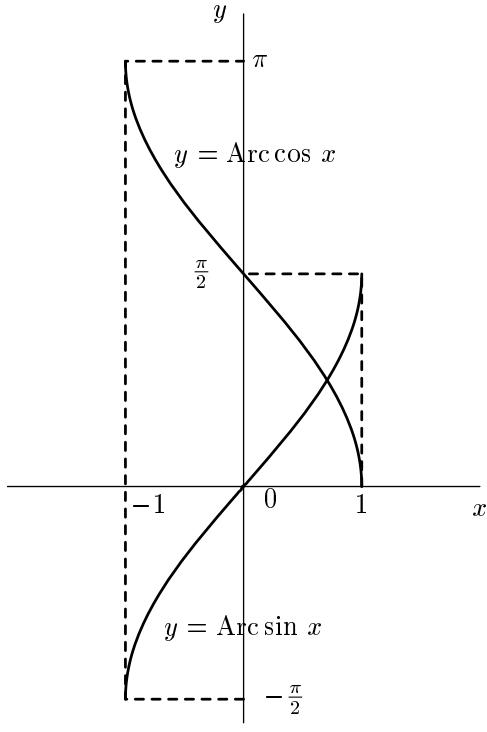
\includegraphics[keepaspectratio]{images/part001_f987f09f.jpg}}\\
图 6

\[
\sin \left(\frac {\pi}{2} - \operatorname{Arc} \cos x\right) = \cos (\operatorname{Arc} \cos x) = x
\]

并且由于 \(-\pi / 2 \leqslant \pi / 2 - \operatorname{Arc} \cos x \leqslant \pi / 2\) ，有

\[
\operatorname{Arc} \cos x = \frac {\pi}{2} - \operatorname{Arc} \sin x\tag{17}
\]

特别由此得出

\[
\mathrm{D} \big (\operatorname{Arc} \cos x \big) = - \frac {1}{\sqrt {1 - x ^ {2}}}.\tag{18}
\]

最后，\(\tan x\) 在区间 \(]-\pi/2, +\pi/2[\) 上的限制是严格递增的；其反函数记作 Arc \(\tan x\) ，它是 R 到 \(]-\pi/2, +\pi/2[\) 上的严格递增映射（图~7）；我们有

\[
\lim _ {x \rightarrow - \infty} \operatorname{Arc} \tan x = - \frac {\pi}{2}, \quad \lim _ {x \rightarrow + \infty} \operatorname{Arc} \tan x = \frac {\pi}{2},
\]

并且，应用反函数求导公式以及 III, p.~95 的公式 (15)，有

\[
\mathrm{D} \big (\operatorname{Arc} \tan x \big) = \frac {1}{1 + x ^ {2}}.\tag{19}
\]

\pandocbounded{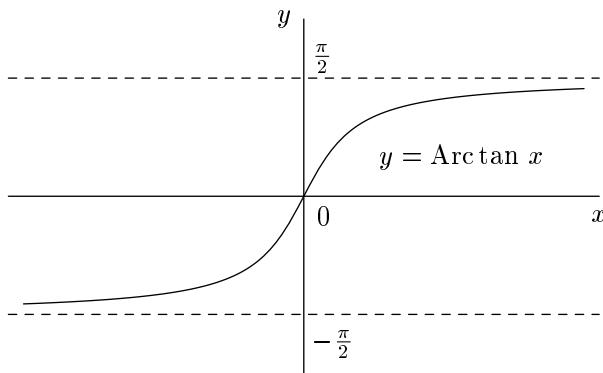
\includegraphics[keepaspectratio]{images/part001_f81b3ea6.jpg}}\\
图 7

\subsection{复指数函数}

我们已在（Gen.~Top., VIII, p.~106）中确定了复数的（加法）拓扑群 C 到（乘法）拓扑群 \(C^{*}\) （由 \(\neq 0\) 的复数组成）上的所有连续同态；它们是映射

\[
x + i y \mapsto e ^ {\alpha x + \beta y} \mathbf {e} (\gamma x + \delta y)\tag{20}
\]

其中 \(\alpha, \beta, \gamma, \delta\) 是满足唯一条件 \(\alpha\delta - \beta\gamma \neq 0\) 的四个实数。我们现在要确定这些同态 \(z \mapsto f(z)\) 中哪些在 C 上可导。首先注意，只需 f 在点 z = 0 可导即可；事实上，对每一点 \(z \in C\) 有 \(\frac{f(z + h) - f(z)}{h} = f(z) \frac{f(h) - 1}{h}\) ；若 \(f'(0)\) 存在，则 \(f'(z)\) 也存在，且 \(f'(z) = af(z)\) ，其中 \(a = f'(0)\) 。另一方面，若 g 是第二个可导同态，满足 \(g'(z) = bg(z)\) ，则 \(g(az/b) = f(z)\) ，因为立即可以看出商 \(g(az/b)/f(z)\) 的导数处处为零且在 z = 0 处等于 1；因此所有可导同态都具有 \(z \mapsto f(\lambda z)\) 的形式，其中 f 是它们中的某一个（假定它们存在），而 \(\lambda\) 是任意（复）常数。

在此情形下，若 \(f\) 在点 \(z = 0\) 可导，则映射 \(x \mapsto f(x)\) 与 \(y \mapsto f(iy)\) （都是 \(\mathbf{R}\) 到 \(\mathbf{C}\) 中的映射）都必在点 0 可导，前者的导数为 \(f'(0)\) ，后者的导数为 \(if'(0)\) 。而映射 \(x \mapsto e^{\alpha x}\mathbf{e}(\gamma x)\) 与 \(y \mapsto e^{\beta y}\mathbf{e}(\delta y)\) 在点 0 的导数分别等于 \(\alpha + 2\pi i\gamma\) 与 \(\beta + 2\pi i\delta\) ，由此得 \(\beta = -2\pi\gamma\) 与 \(\alpha = 2\pi\delta\) ；这些条件特别地为同态 \(x + iy \mapsto e^x\mathbf{e}(y/2\pi)\) 所满足，我们暂时把它记作 \(f_0\) 。现在证明 \(f_0\) 确实在点 \(z = 0\) 可导。

显然 \(x \mapsto f_0(x)\) 与 \(y \mapsto f_0(iy)\) 有各阶导数；特别地，对这两个函数应用 1 阶泰勒公式可知，对每个 \(\varepsilon > 0\) 存在 \(r > 0\) ，使得若令

\[
f _ {0} (x) = 1 + x + \varphi (x) x, \quad f _ {0} (i y) = 1 + i y + \psi (y) y,
\]

则条件 \(|x| \leqslant r, |y| \leqslant r\) 蕴含 \(|\varphi(x)| \leqslant \varepsilon\) 与 \(|\psi(y)| \leqslant \varepsilon\) ；在此情形下，有 \(f_0(x + iy) = f_0(x)f_0(iy) = 1 + (x + iy) + \theta(x, y)\) ，其中

\[
\theta (x, y) = \bigl (i + \varphi (x) \psi (y) \bigr) x y + (1 + x) y \psi (y) + (1 + i y) x \varphi (x);
\]

当 \(|z| \leqslant r\) 时有 \(|x| \leqslant r\) 与 \(|y| \leqslant r\) ，从而

\[
\left| \theta (x, y) \right| \leqslant \left(1 + \varepsilon^ {2}\right) | z | ^ {2} + 2 \varepsilon | z | (1 + | z |)
\]

这证明商 \(\frac{f_{0}(z)-1-z}{z}\) 随 z 趋于 0 而趋于 0 ，也就是说，函数 \(f_{0}\) 在点 z=0 处有导数，等于 1 。于是上面证明了，对一切 \(z\in C\) ，

\[
\mathrm{D} \big (f _ {0} (z) \big) = f _ {0} (z).\tag{21}
\]

这一性质建立了 \(f_{0}\) 与函数 \(e^{x}\) 之间的联系，后者正是 \(f_{0}\) 在实轴上的限制；为此我们给出下面的定义：

定义 2. 同态 \(x + iy \mapsto e^x\mathbf{e}(y/2\pi)\) （\(\mathbf{C}\) 到 \(\mathbf{C}^*\) 上的）称为复指数（函数）；它在任意复数 \(z\) 处的值记作 \(e^z\) 或 \(\exp z\) 。

\subsection{\texorpdfstring{函数 \(e^{z}\) 的性质}{函数 e 的 z 次幂的性质}}

\(z \mapsto e^z\) 是 \(\mathbf{C}\) 到 \(\mathbf{C}^*\) 上的同态，这一事实可用下列恒等式表达

\[
e ^ {z + z ^ {\prime}} = e ^ {z} e ^ {z ^ {\prime}}, \qquad e ^ {0} = 1, \qquad e ^ {- z} = 1 / e ^ {z}.\tag{22}
\]

按定义，对每个 \(z = x + iy\) ，有

\[
e ^ {x + i y} = e ^ {x} (\cos y + i \sin y)\tag{23}
\]

并且由于 \(e^x > 0\) ，可见 \(e^z\) 的绝对值为 \(e^x\) ，辐角为 \(y\) （模 \(2\pi\) ）。

特别地，定义 2（III, p.~98）给出

\[
\mathbf {e} (x) = e ^ {2 \pi i x}\tag{24}
\]

它使我们可以把定义 \(\cos x\) 与 \(\sin x\) 的公式写成如下形式

\[
\cos x = \frac {1}{2} \left(e ^ {i x} + e ^ {- i x}\right), \quad \sin x = \frac {1}{2 i} \left(e ^ {i x} - e ^ {- i x}\right)\tag{25}
\]

（欧拉公式）。

由于 \(2\pi\) 是 \(\mathbf{e}(y/2\pi)\) 的最小周期，\(2\pi i\) 是 \(e^{z}\) 的最小周期；换句话说，\(e^{z}\) 的周期群是数 \(2n\pi i\) 所成的集，其中 n 跑遍 Z。

最后，III, p.~98 的公式 (21) 可写成

\[
\mathrm{D} \left(e ^ {z}\right) = e ^ {z}\tag{26}
\]

从而，对每个复数 \(a\)

\[
\mathrm{D} \big (e ^ {a z} \big) = a e ^ {a z}.\tag{27}
\]

注。若在公式 (27) 中把函数 \(e^{az}\) （a 为复数）限制在实轴上，则对实数 x 再次得到

\[
\mathrm{D} (e ^ {a x}) = a e ^ {a x}.\tag{28}
\]

这个公式使我们可以对 \(e^{\alpha x} \cos \beta x\) ，\(e^{\alpha x} \sin \beta x\) （\(\alpha\) 与 \(\beta\) 为实数）中的每一个函数求出原函数；事实上，我们有 \(e^{(\alpha + i\beta)x} = e^{\alpha x} \cos \beta x + ie^{\alpha x} \sin \beta x\) ，于是由 (28)

\[
\begin{array}{l} \mathrm{D} \left(\mathcal {R} \left(\frac {1}{\alpha + i \beta} e ^ {(\alpha + i \beta) x}\right)\right) = e ^ {\alpha x} \cos \beta x \\ \mathrm{D} \left(\mathcal {I} \left(\frac {1}{\alpha + i \beta} e ^ {(\alpha + i \beta) x}\right)\right) = e ^ {\alpha x} \sin \beta x. \end{array}
\]

同样，可以把求 \(x^n e^{\alpha x} \cos \beta x\) 或 \(x^n e^{\alpha x} \sin \beta x\) （ \(n\) 为整数 \(> 0\) ）的原函数归结为求 \(x^n e^{(\alpha + i\beta)x}\) 的原函数；而 \(n + 1\) 阶分部积分公式（II, p.~60，公式 (11)）表明，后一函数的一个原函数是

\[
e ^ {(\alpha + i \beta) x} \left[ \frac {x ^ {n}}{\alpha + i \beta} - \frac {n x ^ {n - 1}}{(\alpha + i \beta) ^ {2}} + \frac {n (n - 1) x ^ {n - 2}}{(\alpha + i \beta) ^ {3}} + \dots + (- 1) ^ {n} \frac {n !}{(\alpha + i \beta) ^ {n + 1}} \right].
\]

另一方面，利用欧拉公式可以把 \(\cos x\) 或 \(\sin x\) 的每个正整数次幂表示为指数函数 \(e^{ipx}\) （ \(p\) 为正或负整数）的线性组合。于是由公式 (28)，可以把形如 \(x^n e^{\alpha x}(\cos \beta x)^r (\sin \gamma x)^s\) 的函数的原函数表示成形如 \(x^p e^{\alpha x}\cos \lambda x\) 与 \(x^p e^{\alpha x}\sin \mu x\) 的函数的线性组合（\((n, p, r, s\) 为整数，\(\alpha, \beta, \gamma, \lambda, \mu\) 为实数）。

例。有

\[
\sin^ {2 n} x = \frac {(- 1) ^ {n}}{2 ^ {2 n}} \left(e ^ {i x} - e ^ {- i x}\right) ^ {2 n} = \frac {(- 1) ^ {n}}{2 ^ {2 n}} \left(e ^ {2 n i x} - \binom {2 n} {1} e ^ {(2 n - 2) i x} + \dots + e ^ {- 2 n i x}\right)
\]

由此得

\[
\begin{array}{l} \int_ {0} ^ {x} \sin^ {2 n} t d t = \frac {(- 1) ^ {n}}{2 ^ {2 n}} \left(\frac {1}{n} \sin 2 n x - \binom {2 n} {1} \frac {1}{n - 1} \sin (2 n - 2) x + \dots \right. \\ \qquad \qquad \qquad \qquad \qquad \qquad \qquad \qquad \qquad \qquad + (- 1) ^ {n - 1} \binom {2 n} {n - 1} \sin 2 x + (- 1) ^ {n} \binom {2 n} {n} x \Bigg) \end{array}
\]

特别地，

\[
\int_ {0} ^ {\pi / 2} \sin^ {2 n} t   d t = \binom {2 n} {n} \frac {1}{2 ^ {2 n}}   \frac {\pi}{2} = \frac {1 . 3 . 5 \ldots (2 n - 1)}{2 . 4 . 6 \ldots 2 n}   \frac {\pi}{2}.\tag{29}
\]

\subsection{复对数}

设 B 是由点 \(z = x + iy\) （满足 \(-\pi \leqslant y < \pi\) ）所成的“带形”；函数 \(e^{z}\) 在 B 上取它的每个值一次且仅一次；换句话说，\(z \mapsto e^{z}\) 是 B 到 \(C^{*}\) 上的连续双射；在此映射下，（半开）线段 \(x = x_{0}\) ，\(-\pi \leqslant y < \pi\) 的像是圆 \(|z| = e^{x_{0}}\) ；直线 \(y = y_{0}\) 的像是由 \(\operatorname{Am}(z) = y_{0} \pmod{2\pi}\) 定义的（开）半直线。在映射 \(z \mapsto e^{z}\) 下，B 的内部 B （即 \(z \in C\) 中满足 \(|\mathcal{I}(z)| < \pi\) 者所成的集）的像是（闭的）负实半轴在 C 中的余集 F；若约定用 \(\operatorname{Am}(z)\) 表示属于 \([-\pi, \pi]\) 的 z 的辐角量度，则集 F 可由关系 \(-\pi < \operatorname{Am}(z) < \pi\) 定义。由于 \(z \mapsto e^{z}\) 是 C 到 \(C^{*}\) 上的严格同态，任一含于 B 的开集（从而含于 C）在此映射下的像是 \(C^{*}\) 中（从而是 F 中）的开集；换句话说，\(z \mapsto e^{z}\) 在 B 上的限制是 B 到 F 上的同胚。我们把后者的逆同胚，即 F 到 B 上的同胚记作 \(z \mapsto \log z\) ；对复数 \(z \in F\) ，\(\log z\) 称为 z 的对数的主值。若 \(z = x + iy\) 且 \(\log z = u + iv\) ，则 \(x + iy = e^{u + iv}\) ，由此 \(e^{u} = |z|\) ，并且由于 \(-\pi < v < \pi\) ，有 \(v = \operatorname{Am}(z)\) 。此外，有 \(\tan(v + \pi/2) = -x/y\) （若 \(y \neq 0\) ）；于是可以写出

\[
\left\{ \begin{array}{l l} u = \log | z | = \frac {1}{2} \log (x ^ {2} + y ^ {2}) \\ v = \frac {\pi}{2} - \operatorname{Arc} \tan \frac {x}{y} & \text { if } y > 0 \\ v = 0 & \text { if } y = 0 \\ v = - \frac {\pi}{2} - \operatorname{Arc} \tan \frac {x}{y} & \text { if } y <   0. \end{array} \right.\tag{30}
\]

显然 \(\log z\) 是函数 \(\log x\) （定义在正开实半轴 \(R_{+}^{*}\) 上）到 F 上的延拓。若 z，\(z'\) 是 F 中使 \(zz'\) 非负实数的两点，则有 \(\log(zz') = \log z + \log z' + 2\varepsilon\pi i\) ，其中 \(\varepsilon = +1\) 、-1 或 0，视 \(\mathrm{Am}(z)\) 与 \(\mathrm{Am}(z')\) 的值而定。

我们注意，在负实半轴的各点处函数 \(\log z\) 没有极限；确切地说，若 x 趋于 \(x_{0} < 0\) 且 y 保持 \textgreater{} 0（相应地，\textless{} 0）地趋于 0，则 \(\log z\) 趋于 \(\log |x_{0}| + \pi i\) （相应地，\(\log |x_{0}| - \pi i\) ）；当 z 趋于 0 时，\(|\log z|\) 无限增大。

以后我们将看到，解析函数理论如何使我们能把函数 \(\log z\) 延拓，并在完全一般的意义下定义复对数。

由于 \(\log z\) 是 \(e^{z}\) 的逆同胚，反函数求导公式（I, p.~9, prop. 6）表明 \(\log z\) 在每一点 \(z \in F\) 处可导，并且

\[
\mathrm{D} (\log z) = \frac {1}{e ^ {\log z}} = \frac {1}{z}\tag{31}
\]

这个公式推广了 III, p.~93 的公式 (10)。

\subsection{有理函数的原函数}

公式 (31) 使我们能够求出实变量 x 的任意有理函数 \(r(x)\) （系数为实的或复的）的原函数。我们知道（A.VII.7），这样的函数可以（以唯一的方式）写成有限多项之和，这些项是：

\begin{enumerate}
\def\labelenumi{\alph{enumi})}
\item
  或者形如 \(ax^{p}\) （p 为整数 \(\geqslant 0\) ，a 为复数）；
\item
  或者形如 \(a/(x - b)^{m}\) （m 为整数 \(\geqslant 0\) ，a 与 b 为复数）。
\end{enumerate}

现在，容易求出其中每一项的原函数：

\begin{enumerate}
\def\labelenumi{\alph{enumi})}
\tightlist
\item
  \(ax^p\) 的原函数是 \(a\frac{x^{p + 1}}{p + 1}\) ；
\end{enumerate}

\(b)\) 若 \(m > 1\) ，\(a / (x - b)^{m}\) 的原函数是 \(\frac{a}{(1 - m)(x - b)^{m - 1}}\) ；

\begin{enumerate}
\def\labelenumi{\alph{enumi})}
\setcounter{enumi}{2}
\tightlist
\item
  最后，由公式 (10)（III, p.~93）与 (31)（III, p.~101），\(\frac{a}{x - b}\) 的原函数是 \(a\log |x - b|\) （若 \(b\) 为实数），是 \(a\log (x - b)\) （若 \(b\) 为复数）。在后一情形，若 \(b = p + iq\) ，则还有（III, p.~100，公式 (30)）
\end{enumerate}

\[
\log (x - b) = \log \sqrt {(x - p) ^ {2} + q ^ {q}} + i \operatorname{Arc} \tan \frac {x - p}{q} \pm i \frac {\pi}{2}.
\]

我们把更实用的、明显地求出显式给出的有理函数的原函数的方法的考察，推迟到本丛书专讲数值计算的部分。

下列求原函数的问题都可以归结为求有理函数的原函数：

\(1^{\circ}\) 求形如 \(r(e^{ax})\) 的函数的原函数，其中 \(r\) 是有理函数而 \(a\) 是实数；事实上，通过变量替换 \(u = e^{ax}\) ，可归结为求 \(r(u) / u\) 的原函数；

\(2^{\circ}\) 求形如 \(f(\sin ax, \cos ax)\) 的函数的原函数，其中 \(f\) 是两个变量的有理函数而 \(a\) 是实数；变量替换 \(u = \tan(ax/2)\) 把它归结为求下列函数的原函数

\[
{\frac {2}{1 + u ^ {2}}} f \left({\frac {2 u}{1 + u ^ {2}}}, {\frac {1 - u ^ {2}}{1 + u ^ {2}}}\right).
\]

\subsection{复圆函数；双曲函数}

欧拉公式 (25)（III, p.~99）与 \(e^z\) （对每个复数 \(z\) 而言）的定义，使我们可以向 \(\mathbf{C}\) 延拓函数 \(\cos x\) 与 \(\sin x\) ——它们定义在 \(\mathbf{R}\) 上——，只需对一切 \(z \in \mathbf{C}\) 令

\[
\cos z = \frac {1}{2} \left(e ^ {i z} + e ^ {- i z}\right), \quad \sin z = \frac {1}{2 i} \left(e ^ {i z} - e ^ {- i z}\right)\tag{32}
\]

（cf.~III, p.~119, exerc. 19）。

这些函数是以 \(2\pi\) 为最小周期的周期函数；即有 \(\cos(z + \pi/2) = -\sin z\) ，\(\sin(z + \pi/2) = \cos z\) ；还可以验证恒等式

\[
\begin{array}{c} \cos^ {2} z + \sin^ {2} z = 1 \\ \cos (z + z ^ {\prime}) = \cos z \cos z ^ {\prime} - \sin z \sin z ^ {\prime} \\ \sin (z + z ^ {\prime}) = \sin z \cos z ^ {\prime} + \cos z \sin z ^ {\prime}. \end{array}
\]

更一般地，实变量圆函数之间的每个代数恒等式当这些变量取任意复值时仍然成立（III, p.~119, exerc. 18）。

令 \(\tan z = \sin z/\cos z\) （若 \(z \neq (2k + 1)\pi/2\) ），令 \(\cot z = \cos z/\sin z\) （若 \(z \neq k\pi\) ）；它们是以 \(\pi\) 为最小周期的周期函数。

公式 (27)（III, p.~99）表明 \(\cos z\) 与 \(\sin z\) 在 \(\mathbf{C}\) 上可导，并且

\[
\mathrm{D} (\cos z) = - \sin z, \quad \mathrm{D} (\sin z) = \cos z.
\]

对 \(z = ix\) （x 为实数），公式 (32) 给出

\[
\cos i x = \frac {1}{2} \left(e ^ {x} + e ^ {- x}\right), \quad \sin i x = \frac {i}{2} \left(e ^ {x} - e ^ {- x}\right).
\]

对这样引入的实函数，采用专门的记号是方便的；我们令

\[
\left\{ \begin{array}{l l} \cosh x = \frac {1}{2} \left(e ^ {x} + e ^ {- x}\right) & \text {(hyperbolic cosine of x)} \\ \sinh x = \frac {i}{2} \left(e ^ {x} - e ^ {- x}\right) & \text {(hyperbolic sine of x)} \\ \tanh x = \frac {\sinh x}{\cosh x} = \frac {e ^ {x} - e ^ {- x}}{e ^ {x} + e ^ {- x}} & \text {(hyperbolic tangent of x)} \end{array} \right.\tag{33}
\]

于是，对每个实数 \(x\)

\[
\cos i x = \cosh x, \quad \sin i x = i \sinh x.\tag{34}
\]

由若干复数 \(z_{k}\) （ \(1 \leqslant k \leqslant n\) ）的圆函数之间的每个恒等式，把 \(z_{k}\) 换成 \(ix_{k}\) （ \(x_{k}\) 为实数，\(1 \leqslant k \leqslant n\) ）并利用公式 (34)，就可以得到双曲函数的一个恒等式；例如有

\[
\begin{array}{c} \cosh^ {2} x - \sinh^ {2} x = 1 \\ \cosh (x + x ^ {\prime}) = \cosh x \cosh x ^ {\prime} + \sinh x \sinh x ^ {\prime} \\ \sinh (x + x ^ {\prime}) = \sinh x \cosh x ^ {\prime} - \cosh x \sinh x ^ {\prime}. \end{array}
\]

双曲函数使我们可以表出 \(\cos z\) 与 \(\sin z\) 当 \(z = x + iy\) 时的实部与虚部，因为

\[
\begin{array}{l} \cos (x + i y) = \cos x \cos i y - \sin x \sin i y = \cos x \cosh y - i \sin x \sinh y \\ \sin (x + i y) = \sin x \cos i y + \cos x \sin i y = \sin x \cosh y + i \cos x \sinh y. \end{array}
\]

最后，有

\[
\mathrm{D} (\cosh x) = \sinh x, \mathrm{D} (\sinh x) = \cosh x, \mathrm{D} (\tanh x) = 1 - \tanh ^ {2} x = \frac {1}{\cosh^ {2} x}.
\]

由于对一切 x 有 \(\cosh x > 0\) ，由此推出 \(\sinh x\) 在 R 上严格递增；又 \(\sinh 0 = 0\) ，故 \(\sinh x\) 与 x 同号。于是 \(\cosh x\) 在 \(x \leqslant 0\) 时严格递减，在 \(x \geqslant 0\) 时严格递增；最后，\(\tanh x\) 在 R 上严格递增。此外

\[
\begin{array}{l} \lim _ {x \to - \infty} \sinh x = - \infty , \quad \lim _ {x \to + \infty} \sinh x = + \infty \\ \lim _ {x \to - \infty} \cosh x = \lim _ {x \to + \infty} \cosh x = + \infty \\ \lim _ {x \to - \infty} \tanh x = - 1, \quad \lim _ {x \to + \infty} \tanh x = + 1 \quad (\text {   fig.   8   and   9   }). \end{array}
\]

有时以 \(\operatorname{Arg}\sinh x\) 表示 \(\sinh x\) 的反函数，它是 \(\mathbf{R}\) 到 \(\mathbf{R}\) 上的严格递增映射；这个函数也可以用对数表示，因为由关系式 \(x = \sinh y = \frac{1}{2}(e^y - e^{-y})\) 推出 \(e^{2y} - 2xe^y - 1 = 0\) ，而由于 \(e^y > 0\) ，有 \(e^y = x + \sqrt{x^2 + 1}\) ，也就是说

\[
\operatorname{Arg} \sinh x = \log (x + \sqrt {x ^ {2} + 1}).
\]

类似地，我们把 \(\operatorname{Arg}\cosh x\) 记为 \(\cosh x\) 在 \([0, +\infty[\) 上的限制的反函数；这个映射是 \([1, +\infty[\) 到 \([0, +\infty[\) 上的严格递增映射；与上面一样可以证明

\[
\operatorname{Arg} \cosh x = \log (x + \sqrt {x ^ {2} - 1}).
\]

\pandocbounded{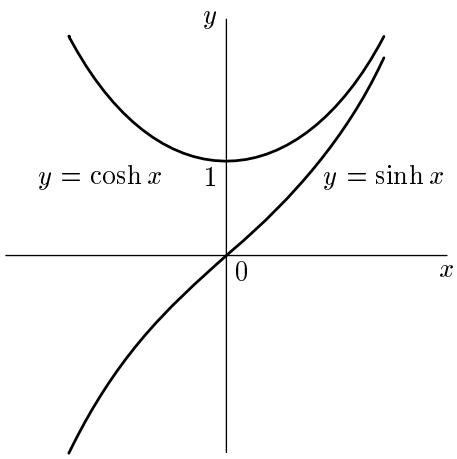
\includegraphics[keepaspectratio]{images/part001_d9e35212.jpg}}\\
图 8

\pandocbounded{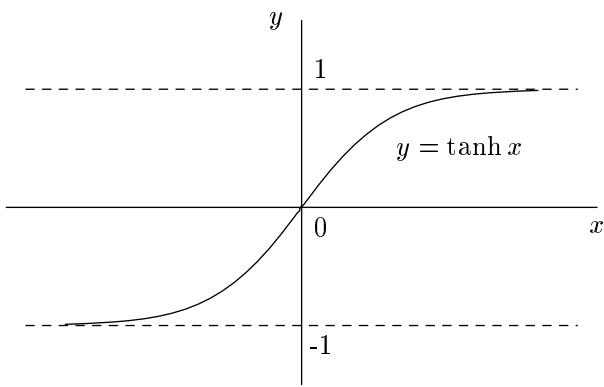
\includegraphics[keepaspectratio]{images/part001_f5896466.jpg}}\\
图 9

最后，我们以 \(\operatorname{Arg}\tanh x\) 表示 \(\tanh x\) 的反函数，它是 \(] - 1, +1[\) 到 \(\mathbf{R}\) 上的严格递增映射；此外有

\[
\operatorname{Arg} \tanh x = \frac {1}{2} \log \frac {1 + x}{1 - x}.
\]

注。对复数 \(z\) ，有时写

\[
\begin{array}{l} \cosh z = \frac {1}{2} (e ^ {z} + e ^ {- z}) = \cos i z \\ \sinh z = \frac {1}{2} (e ^ {z} - e ^ {- z}) = - i \sin i z. \end{array}
\]

这些函数就这样把定义在 R 上的双曲函数延拓到了 C。

\section{指数函数、圆函数及其相关函数的展开}

\subsection{实指数函数的展开}

由于 \(\mathrm{D}^n (e^x) = e^x\) ，按 \(n\) 阶泰勒展开，\(e^x\) 为

\[
e ^ {x} = 1 + \frac {x}{1 !} + \frac {x ^ {2}}{2 !} + \dots + \frac {x ^ {n}}{n !} + \int_ {0} ^ {x} \frac {(x - t) ^ {n}}{n !} e ^ {t} d t.\tag{1}
\]

这个公式的余项 \(>0\) （当 \(x > 0\) ），且有 \((-1)^{n + 1}\) 的符号（当 \(x < 0\) ）；此外，中值不等式表明

\[
\frac {x ^ {n + 1}}{(n + 1) !} <   \int_ {0} ^ {x} \frac {(x - t) ^ {n}}{n !} e ^ {t} d t <   \frac {x ^ {n + 1} e ^ {x}}{(n + 1) !} \quad \text { for } x > 0\tag{2}
\]

\[
\frac {\left| x ^ {n + 1} \right| e ^ {x}}{(n + 1) !} <   \left| \int_ {0} ^ {x} \frac {(x - t) ^ {n}}{n !} e ^ {t} d t \right| <   \frac {\left| x ^ {n + 1} \right|}{(n + 1) !} \quad \text { for } x <   0\tag{3}
\]

现在我们知道，序列 \((x^{n}/n!)\) 当 n 无限增大时以 0 为极限（对一切 \(x \geqslant 0\) ；Gen.~Top., IV, p.~365）；于是，在 (1) 中固定 x 而让 n 无限增大，由 (2) 与 (3) 就得出

\[
e ^ {x} = \sum_ {n = 0} ^ {\infty} \frac {x ^ {n}}{n !}\tag{4}
\]

并且右端的级数在 \(\mathbf{R}\) 的每个紧区间上绝对且一致收敛。特别地，有公式

\[
e = 1 + \frac {1}{1 !} + \frac {1}{2 !} + \dots + \frac {1}{n !} + \dots\tag{5}
\]

这个公式使我们可以计算出与数 \(e\) 任意接近的有理近似值；我们得到

\[
e = 2. 7 1 8   2 8 1   8 2 8 \dots
\]

精确到 \(1/10^{9}\) 。此外，公式 (5) 证明 e 是无理数 \(^{2}\) （Gen.~Top., IV, p.~375）。

注。由于公式 (1) 的余项 \textgreater0 （当 x \textgreater{} 0 时），故对 x \textgreater{} 0 有

\[
e ^ {x} > 1 + \frac {x}{1 !} + \frac {x ^ {2}}{2 !} + \dots + \frac {x ^ {n + 1}}{(n + 1) !}
\]

因而更有

\[
e ^ {x} > \frac {x ^ {n + 1}}{(n + 1) !}
\]

对每个整数 \(n\) 成立：由此推出，\(e^x / x^n\) 以 \(+\infty\) 为极限（当 \(x\) 无限增大时；对每个整数 \(n\) ）：我们将在第 V 章中用另一种方法再次得到这一结果（V, p.~231）。

\subsection{\texorpdfstring{复指数函数、\(\cos x\) 与 \(\sin x\) 的展开。}{复指数函数、cos x 与 sin x 的展开。}}

设 z 是任意复数，考虑实变量 t 的函数 \(\varphi(t) = e^{zt}\) ；我们有 \(\mathrm{D}^{n}\varphi(t) = z^{n}e^{zt}\) 与 \(e^{z} = \varphi(1)\) ；于是，用 \(\varphi(1)\) 在点 t = 0 处的 n 阶泰勒公式来表示它（II, p.~62），便得

\[
e ^ {z} = 1 + \frac {z}{1 !} + \frac {z ^ {2}}{2 !} + \dots + \frac {z ^ {n}}{n !} + z ^ {n + 1} \int_ {0} ^ {1} \frac {(1 - t) ^ {n}}{n !} e ^ {z t} d t\tag{6}
\]

当 \(z\) 为实数时这个公式与 (1) 等价。余项

\[
r _ {n} (z) = z ^ {n + 1} \int_ {0} ^ {1} \frac {(1 - t) ^ {n}}{n !} e ^ {z t} d t
\]

的绝对值可用中值不等式从上方控制；若 \(z = x + iy\) ，我们有 \(|e^{zt}| = e^{xt}\) ，于是 \(|e^{zt}| \leqslant 1\) （当 \(x \leqslant 0\) ），\(|e^{zt}| \leqslant e^x\) （当 \(x > 0\) ）；因此

\[
\left| r _ {n} (z) \right| \leqslant \frac {\left| z \right| ^ {n + 1}}{(n + 1) !} \text {   if   } x \leqslant 0\tag{7}
\]

\[
| r _ {n} (z) | \leqslant \frac {| z | ^ {n + 1} e ^ {x}}{(n + 1) !} \text {   if   } x > 0.\tag{8}
\]

与上面一样，我们得出

\[
e ^ {z} = \sum_ {n = 0} ^ {\infty} \frac {z ^ {n}}{n !}\tag{9}
\]

该级数在 \(\mathbf{C}\) 的每个紧子集上绝对且一致收敛。由 (6) 特别得出

\[
e ^ {i x} = 1 + \frac {i x}{1 !} + \frac {i ^ {2} x ^ {2}}{2 !} + \dots + \frac {i ^ {n} x ^ {n}}{n !} + i ^ {n + 1} \int_ {0} ^ {x} \frac {(x - t) ^ {n}}{n !} e ^ {i t} d t\tag{10}
\]

由此可得 \(\cos x\) 与 \(\sin x\) 的泰勒展开；取 (10) 的 \(2n + 1\) 阶实部便得

\[
\cos x = 1 - \frac {x ^ {2}}{2 !} + \dots + (- 1) ^ {n} \frac {x ^ {2 n}}{(2 n) !} + (- 1) ^ {n + 1} \int_ {0} ^ {x} \frac {(x - t) ^ {2 n + 1}}{(2 n + 1) !} \cos t d t\tag{11}
\]

其余项满足界

\[
\left| \int_ {0} ^ {x} \frac {(x - t) ^ {2 n + 1}}{(2 n + 1) !} \cos t d t \right| \leqslant \frac {| x | ^ {2 n + 2}}{(2 n + 2) !}.\tag{12}
\]

类似地，取 (10) 的 \(2n\) 阶虚部，我们得到

\[
\begin{array}{l} \sin x = x - \frac {x ^ {3}}{3 !} + \frac {x ^ {5}}{5 !} + \dots + (- 1) ^ {n - 1} \frac {x ^ {2 n - 1}}{(2 n - 1) !} \\ \qquad + (- 1) ^ {n} \int_ {0} ^ {x} \frac {(x - t) ^ {2 n}}{(2 n) !} \cos t d t \end{array}\tag{13}
\]

其余项满足界

\[
\left| \int_ {0} ^ {x} \frac {(x - t) ^ {2 n}}{(2 n) !} \cos t d t \right| \leqslant \frac {| x | ^ {2 n + 1}}{(2 n + 1) !}.\tag{14}
\]

此外，比较 (11) 中 \(2n + 1\) 阶与 \(2n + 3\) 阶的余项，有

\[
\int_ {0} ^ {x} \frac {(x - t) ^ {2 n + 3}}{(2 n + 3) !} \cos t d t = \frac {x ^ {2 n + 2}}{(2 n + 2) !} - \int_ {0} ^ {x} \frac {(x - t) ^ {2 n + 1}}{(2 n + 1) !} \cos t d t
\]

并把 (12) 考虑在内，便知不论 x 为何值，(11) 的余项都有与 \((-1)^{n+1}\) 相同的符号；同样可以证明 (13) 的余项与 \((-1)^{n}x\) 同号。特别地，在 (11) 中取 n = 0 与 n = 1，在 (13) 中取 n = 1 与 n = 2，就得到不等式

\[
1 - \frac {x ^ {2}}{2} \leqslant \cos x \leqslant 1 \quad \text { for   all } x\tag{15}
\]

\[
x - \frac {x ^ {3}}{6} \leqslant \sin x \leqslant x \quad \text { for   all } x \geqslant 0.\tag{16}
\]

最后，在 (9) 中令 z = ix 便得

\[
\cos x = \sum_ {n = 0} ^ {\infty} (- 1) ^ {n} \frac {x ^ {2 n}}{(2 n) !}\tag{17}
\]

\[
\sin x = \sum_ {n = 0} ^ {\infty} (- 1) ^ {n} \frac {x ^ {2 n + 1}}{(2 n + 1) !}\tag{18}
\]

这些级数在每个紧区间上绝对且一致收敛。

此外，显然公式 (17) 与 (18) 对每个复数 x 仍然成立，右端的级数在 C 的每个紧子集上绝对且一致收敛。特别地，对每个 x（实的或复的）

\[
\begin{array}{l} \cosh x = \sum_ {n = 0} ^ {\infty} \frac {x ^ {2 n}}{(2 n) !} \\ \sinh x = \sum_ {n = 0} ^ {\infty} \frac {x ^ {2 n + 1}}{(2 n + 1) !}. \end{array}
\]

\subsection{二项展开}

设 \(m\) 是任意实数。对 \(x > 0\) 我们有

\[
\mathrm{D} ^ {n} (x ^ {m}) = m (m - 1) \dots (m - n + 1) x ^ {m - n};
\]

把 \(n\) 阶泰勒公式（关于点 \(x = 0\) ）应用于函数 \((1 + x)^m\) ，便知对每个 \(x > -1\)

\[
(1 + x) ^ {m} = 1 + \binom {m} {1} x + \binom {m} {2} x ^ {2} + \dots + \binom {m} {n} x ^ {n} + r _ {n} (x)\tag{19}
\]

其中

\[
r _ {n} (x) = \frac {m (m - 1) \dots (m - n)}{n !} \int_ {0} ^ {x} \left(\frac {x - t}{1 + t}\right) ^ {n} (1 + t) ^ {m - 1} d t
\]

其中令 \(\binom{m}{n} = \frac{m(m-1)\ldots(m-n+1)}{n!}\) 。当 m 是整数 \textgreater{} 0 且 \(n \geqslant m\) 时，公式 (19) 就化为二项式公式（Alg., I, p.~99）；通过推广，我们仍称它为二项式公式，并称系数 \(\binom{m}{n}\) 为二项式系数，这里 m 是任意实数而 n 是任意整数 \textgreater{} 0 。

(19) 的余项与 \(\binom{m}{n+1}\) 同号（当 \(x > 0\) 时），且与 \((-1)^{n+1}\binom{m}{n+1}\) 同号（当 \(-1 < x < 0\) 时）。由于 \(\left|\frac{x-t}{1+t}\right| \leqslant |x|\) 对 \(t > -1\) （在以 0 与 \(x\) 为端点的区间中）成立，故对任意的 \(m\) 、\(n\) 与 \(x > -1\) ，余项满足下面的界：

\[
\begin{array}{r l} \left| \frac {m (m - 1) \dots (m - n)}{n !} \int_ {0} ^ {x} \left(\frac {x - t}{1 + t}\right) ^ {n} (1 + t) ^ {m - 1} d t \right| & \\ & \leqslant \left| \binom {m - 1} {n} x ^ {n} ((1 + x) ^ {m} - 1) \right|. \end{array}\tag{20}
\]

若设 \(x \geqslant 0\) 且 \(n \geqslant m - 1\) ，则在积分区间上 \((1 + t)^{n - m + 1} \geqslant 1\) ，于是

\[
0 \leqslant \int_ {0} ^ {x} \frac {(x - t) ^ {n}}{(1 + t) ^ {n - m + 1}} d t \leqslant \int_ {0} ^ {x} (x - t) ^ {n} d t = \frac {x ^ {n + 1}}{n + 1}
\]

由此得到估计式

\[
\left| r _ {n} (x) \right| \leqslant \left| \binom {m} {n + 1} \right| x ^ {n + 1} \quad (x \geqslant 0, n \geqslant m - 1)\tag{21}
\]

它是对余项的估计。另一方面，设 \(-1 \leqslant m < 0\) ；若在积分 (19) 中作变量替换 \(u = \frac{x - t}{x(1 + t)}\) ，则得

\[
r _ {n} (x) = \frac {m (m - 1) \dots (m - n)}{n !} (1 + x) ^ {m} x ^ {n + 1} \int_ {0} ^ {1} \frac {u ^ {n} d u}{(1 + u x) ^ {m + 1}}.\tag{22}
\]

为对 x \textgreater{} -1 的情形估计该积分，我们注意到：由于 \(m + 1 < 1\) ，积分 \(\int_{0}^{1}\frac{u^{n}du}{(1-u)^{m+1}}\) 收敛，且因 \(1+ux > 1-u\) ，它控制 (22) 的右端。而对 -1 \textless{} x \textless{} 0 ，关于 m 的假设蕴含 (19) 右端出现的所有项 \(\binom{m}{1}x,\binom{m}{2}x^{2},\ldots,\binom{m}{n}x^{n}\) 均 \(\geqslant 0\) ，故 \(r_{n}(x) \leqslant (1+x)^{m}\) ；用 \((1+x)^{m}\) 除之，即得

\[
\frac {m (m - 1) \dots (m - n)}{n !} x ^ {n + 1} \int_ {0} ^ {1} \frac {u ^ {n} d u}{(1 + u x) ^ {m + 1}} \leqslant 1.
\]

此外，当 \(-1 < x < 0\) 时积分号前的因子 \(\geqslant 0\) ，故令 \(x\) 趋于 \(-1\) ，便得

\[
\left| \frac {m (m - 1) \dots (m - n)}{n !} \int_ {0} ^ {1} \frac {u ^ {n} d u}{(1 - u) ^ {m + 1}} \right| \leqslant 1
\]

因而当 \(-1 \leqslant m < 0\) 且 \(x > -1\) 时有

\[
\left| r _ {n} (x) \right| \leqslant (1 + x) ^ {m} | x | ^ {n + 1}.\tag{23}
\]

首先，从这些不等式可以推出：当 \(|x| < 1\) 时有

\[
(1 + x) ^ {m} = \sum_ {n = 0} ^ {\infty} \binom {m} {n} x ^ {n}\tag{24}
\]

其右端（称为二项级数）在 {]} - 1, +1{[} 的每个紧子集上绝对且一致收敛。事实上，可以写出

\[
\binom {m} {n} = (- 1) ^ {n} \left(1 - \frac {m + 1}{1}\right) \left(1 - \frac {m + 1}{2}\right) \dots \left(1 - \frac {m + 1}{n}\right)\tag{25}
\]

由此得

\[
\left| \binom {m} {n} \right| \leqslant \left(1 + \frac {| m + 1 |}{1}\right) \left(1 + \frac {| m + 1 |}{2}\right) \dots \left(1 + \frac {| m + 1 |}{n}\right).
\]

若 \(|x| \leqslant r < 1\) ，则存在 \(n_0\) 使得 \(1 + \frac{|m|}{n_0} < \frac{1}{r'}\) ，其中 \(r < r' < 1\) ；由此，令

\[
k = \left(1 + \frac {| m |}{1}\right) \left(1 + \frac {| m |}{2}\right) \dots \left(1 + \frac {| m |}{n _ {0}}\right)
\]

便有

\[
\left| \binom {m - 1} {n} x ^ {n} \right| \leqslant k | x | ^ {n _ {0}} \left(\frac {r}{r ^ {\prime}}\right) ^ {n - n _ {0}},
\]

这就证明了该命题。另一方面，对 x \textgreater{} 1 ，若 m 不是整数 \(\geqslant 0\) ，则级数 (24) 通项的绝对值随 n 无限增大；事实上，由 (25) 知，对 \(n > n_{1} \geqslant |m + 1|\) 有

\[
\begin{array}{r l} \left| \binom {m} {n} \right| & \geqslant \left| \left(1 - \frac {m + 1}{1}\right) \left(1 - \frac {m + 1}{2}\right) \dots \left(1 - \frac {m + 1}{n _ {1}}\right) \right| \\ & \quad \left(1 - \frac {| m + 1 |}{n _ {1} + 1}\right) \dots \left(1 - \frac {| m + 1 |}{n}\right). \end{array}
\]

取 \(n_0 \geqslant n_1\) 使得当 \(n \geqslant n_0\) 时 \(1 - \frac{|m + 1|}{n} > \frac{1}{x'}\) ，其中 \(1 < x' < x\) 。若令

\[
k ^ {\prime} = \left| \left(1 - \frac {m + 1}{1}\right) \dots \left(1 - \frac {m + 1}{n _ {1}}\right) \right| \left(1 - \frac {| m + 1 |}{n _ {1} + 1}\right) \dots \left(1 - \frac {| m + 1 |}{n _ {0}}\right)
\]

则当 \(n > n_0\) 时

\[
\left| \binom {m} {n} x ^ {n} \right| \geqslant k ^ {\prime} | x | ^ {n _ {0}} \left(\frac {x}{x ^ {\prime}}\right) ^ {n - n _ {0}}
\]

命题由此得证。

我们注意到，当 \(m = -1\) 时，代数恒等式

\[
\frac {1}{1 + x} = 1 - x + x ^ {2} - \dots + (- 1) ^ {n - 1} x ^ {n - 1} + (- 1) ^ {n} \frac {x ^ {n}}{1 + x}\tag{26}
\]

无需积分便给出了普遍公式 (19) 中余项的表达式；这时公式 (23) 化为几何级数（或等比数列）求和的表达式（Gen.~Top., IV, p.~364）。

其次，我们来研究二项级数当 \(x = 1\) 或 \(x = -1\) 时的收敛性（排除平凡情形 \(m = 0\) ）：

\begin{enumerate}
\def\labelenumi{\alph{enumi})}
\item
  \(m \leqslant -1\) 。通项为 \(1 - \frac{m + 1}{n}\) 的乘积趋于 \(+\infty\) （若 \(m < -1\) ），趋于 1 （若 \(m = -1\) ），故由 (25) 知，当 \(x = \pm 1\) 时二项级数的通项不趋于 0。
\item
  -1 \textless{} m \textless{} 0。这时通项为 \(1 - \frac{m + 1}{n}\) 的乘积趋于 0 ，故不等式 (21) 表明 \(r_{n}(1)\) 趋于 0。于是二项级数在 x = 1 处收敛且和为 \(2^{m}\) ；此外，由前文所见及 (21) ，二项级数在每个区间 \([x_{0}, 1]\) （ \(-1 < x_{0} \leqslant 1\) ）上一致收敛。另一方面，当 x = -1 时 (24) 右端所有的项都 \(\geqslant 0\) ；倘若这级数收敛，便可推出二项级数在 \([-1, 1]\) 上正规收敛，从而其和是该区间上的连续函数，而这是荒谬的，因为 \((1 + x)^{m}\) 在 \([-1, 1]\) 上无界（当 m \textless{} 0 时）。由此断定，二项级数在 x = 1 处同样不是绝对收敛的。
\item
  m \textgreater{} 0。\(r_{n}(x)\) 的定义表明，当 x 趋于 -1 时 \(r_{n}(x)\) 趋于极限 \(r_{n}(-1)\) ；在 (20) 中取极限便可断定 \(|r_{n}(-1)| \leqslant \left|\binom{m-1}{n}\right|\) ，又因 m - 1 \textgreater{} -1 ，可见二项级数在 x = -1 处收敛。此外，当 \(n > m + 1\) 时该级数所有的项同号；因而二项级数在区间 \([-1, 1]\) 上正规收敛，且在该区间上的和为 \((1 + x)^{m}\) 。
\end{enumerate}

\subsection{\texorpdfstring{\(\log(1 + x)\)、Arc tan x 与 Arc sin x 的展开}{log(1 + x)、Arc tan x 与 Arc sin x 的展开}}

将 (26) 两端从 0 到 x 积分，即得 \(\log(1 + x)\) 的 n 阶泰勒展开，它对 x \textgreater{} -1 成立

\[
\log (1 + x) = \frac {x}{1} - \frac {x ^ {2}}{2} + \frac {x ^ {3}}{3} + \dots + (- 1) ^ {n - 1} \frac {x ^ {n}}{n} + (- 1) ^ {n} \int_ {0} ^ {x} \frac {t ^ {n} d t}{1 + t}.\tag{27}
\]

余项与 \((-1)^{n}\) 同号（当 x \textgreater{} 0 时），且为 \textless{} 0 （当 -1 \textless{} x \textless{} 0 时）；再者，当 x \textgreater{} 0 时，有 \(1 + t \geqslant 1\) （对 \(0 \leqslant t \leqslant x\) ），而当 -1 \textless{} x \textless{} 0 时，有 \(1 + t \geqslant 1 - |x|\) （对 \(x \leqslant 0\) ）；由此得余项的估计式

\[
\left| \int_ {0} ^ {x} \frac {t ^ {n} d t}{1 + t} \right| \leqslant \frac {| x | ^ {n + 1}}{n + 1}
\]

\[
\text { for } x \geqslant 0\tag{28}
\]

\[
\left| \int_ {0} ^ {x} \frac {t ^ {n} d t}{1 + t} \right| \leqslant \frac {| x | ^ {n + 1}}{(n + 1) (1 - | x |)} \quad \text {   for   } - 1 <   x \leqslant 0.\tag{29}
\]

由最后这两个公式立即可得：当 \(-1 < x \leqslant 1\) 时有

\[
\log (1 + x) = \sum_ {n = 1} ^ {\infty} (- 1) ^ {n - 1} \frac {x ^ {n}}{n}\tag{30}
\]

该级数在含于 \(]-1,+1]\) 的每个紧区间上一致收敛，且当 \(|x|<1\) 时绝对收敛。

另一方面，当 \(|x| > 1\) 时 (30) 右端级数的通项的绝对值随 n 无限增大（III, p.~106）。当 x = -1 时该级数化为调和级数，其和为 \(+\infty\) （Gen.~Top., IV, p.~365）。

类似地，在 (26) 中把 \(x\) 换成 \(x^2\) ，并将两端从 0 到 \(x\) 积分，即得 \(2n - 1\) 阶泰勒展开（对 \(\operatorname{Arctan} x\) ），它对一切实数 \(x\) 成立

\[
\operatorname{Arc} \tan x = \frac {x}{1} - \frac {x ^ {3}}{3} + \frac {x ^ {5}}{5} + \dots + (- 1) ^ {n - 1} \frac {x ^ {2 n - 1}}{2 n - 1} + (- 1) ^ {n} \int_ {0} ^ {x} \frac {t ^ {2 n} d t}{1 + t ^ {2}}.\tag{31}
\]

余项与 \((-1)^n x\) 同号；由于 \(1 + t^2 \geqslant 1\) 对一切 \(t\) 成立，我们有估计式

\[
\left| \int_ {0} ^ {x} \frac {t ^ {2 n} d t}{1 + t ^ {2}} \right| \leqslant \frac {| x | ^ {2 n + 1}}{2 n + 1}\tag{32}
\]

由此推出：当 \(|x| \leqslant 1\) 时

\[
\operatorname{Arc} \tan x = \sum_ {n = 1} ^ {\infty} (- 1) ^ {n - 1} \frac {x ^ {2 n - 1}}{2 n - 1}\tag{33}
\]

该级数在 \([-1,+1]\) 上一致收敛，且当 \(|x|<1\) 时绝对收敛。

特别地，取 \(x = 1\) 便得到公式

\[
{\frac {\pi}{4}} = 1 - {\frac {1}{3}} + {\frac {1}{5}} + \dots + (- 1) ^ {n} {\frac {1}{2 n + 1}} + \dots .\tag{34}
\]

当 \(|x| > 1\) 时 (33) 右端的通项的绝对值随 \(n\) 无限增大。

最后，关于 Arc sin x 的泰勒展开，我们从其导数 \((1 - x^{2})^{-1/2}\) 的展开出发；后一展开是在二项级数展开中以 \(-x^{2}\) 代换 x 而从 \((1 + x)^{-1/2}\) 得到的；对 \(|x| < 1\) 这给出

\[
(1 - x ^ {2}) ^ {- 1 / 2} = 1 + \frac {1}{2} x ^ {2} + \frac {1 . 3}{2 . 4} x ^ {4} + \dots + \frac {1 . 3 . 5 \dots (2 n - 1)}{2 . 4 . 6 \dots 2 n} x ^ {2 n} + r _ {n} (x)
\]

并且由 (23) ，其余项满足界

\[
0 \leqslant r _ {n} (x) \leqslant \frac {x ^ {2 n + 2}}{\sqrt {1 - x ^ {2}}}
\]

此即对余项的界。

取前一展开式的原函数，便得

\[
\operatorname{Arc} \sin x = x + \frac {1}{2} \frac {x ^ {3}}{3} + \frac {1 . 3}{2 . 4} \frac {x ^ {5}}{5} + \dots + \frac {1 . 3 . 5 \dots (2 n - 1)}{2 . 4 . 6 \dots 2 n} \frac {x ^ {2 n + 1}}{2 n + 1} + \mathrm{R} _ {n} (x)\tag{35}
\]

其中 \(\mathrm{R}_{n}(x)\) 与 x 同号且满足不等式

\[
| \mathrm{R} _ {n} (x) | \leqslant \int_ {0} ^ {x} \frac {t ^ {2 n + 2} d t}{\sqrt {1 - t ^ {2}}}.\tag{36}
\]

此外，关系式 (35) 表明 \(\mathbf{R}_n(x)\) 当 \(x\) 趋于 1 或 \(-1\) 时趋于一个极限，故有

\[
| \mathrm{R} _ {n} (1) | \leqslant \int_ {0} ^ {1} \frac {t ^ {2 n + 2} d t}{\sqrt {1 - t ^ {2}}}.\tag{37}
\]

但 (37) 的右端当 \(n\) 趋于 \(+\infty\) 时趋于 0 ：事实上，由于积分 \(\int_0^1 dt / \sqrt{1 - t^2}\) 收敛，对每个 \(\varepsilon > 0\) 存在 \(a\) 满足 \(0 < a < 1\) 且 \(\int_a^1 dt / \sqrt{1 - t^2} \leqslant \varepsilon\) ；另一方面我们有

\[
\int_ {0} ^ {a} \frac {t ^ {2 n + 2} d t}{\sqrt {1 - t ^ {2}}} \leqslant \frac {1}{\sqrt {1 - a ^ {2}}} \int_ {0} ^ {a} t ^ {2 n + 2} d t = \frac {a ^ {2 n + 3}}{(2 n + 3) \sqrt {1 - a ^ {2}}}
\]

于是存在 \(n_0\) ，使得当 \(n \geqslant n_0\) 时 \(\frac{a^{2n+3}}{(2n+3)\sqrt{1-a^2}} \leqslant \varepsilon\) ；由此，最终得 \(|\mathrm{R}_n(x)| \leqslant 2\varepsilon\) （当 \(|x| \leqslant 1\) 且 \(n \geqslant n_0\) ）。于是有

\[
\operatorname{Arc} \sin x = \sum_ {n = 0} ^ {\infty} \frac {1 . 3 . 5 \dots (2 n - 1)}{2 . 4 . 6 \dots 2 n} \frac {x ^ {2 n + 1}}{2 n + 1}\tag{38}
\]

其右端在紧区间 \([-1, 1]\) 上正规收敛。

在相反的情形，可以像对二项级数那样证明：当 \(|x| > 1\) 时 (38) 右端级数的通项的绝对值无限增大。

例如，在 (38) 中取 \(x = \frac{1}{2}\) ，就得到数 \(\pi\) 的一个新表达式；

\[
\frac {\pi}{6} = \sum_ {n = 0} ^ {\infty} \frac {1 . 3 . 5 \dots (2 n - 1)}{2 . 4 . 6 \dots 2 n} \frac {1}{(2 n + 1) 2 ^ {2 n + 1}}
\]

它比公式 (34) 更适合于计算 \(\pi\) 的近似值（参见 Calcul numérique）；由此得到

\[
\pi = 3. 1 4 1   5 9 2   6 5 3 \dots
\]

精确到 \(1/10^{9}\) 。\(^{3}\)

\setcounter{exercisegroup}{0}
\refstepcounter{exercisegroup}
\section*{第 \S\arabic{exercisegroup} 节习题}
\phantomsection
\addcontentsline{toc}{section}{第 \protect\S\arabic{exercisegroup} 节习题}

\begin{enumerate}
\def\labelenumi{\arabic{enumi})}
\item
  设 \(\mathbf{f}\) 是 \(\mathbf{R}\) 到 \(\mathbf{R}\) 上的一个具有单位元 \(\mathbf{e}\) 的完备赋范代数 E 中的连续且可导的映射；假设 \(\mathbf{f}(0) = \mathbf{e}\) ，并且恒有 \(\mathbf{f}'(x) = \mathbf{f}(x)\mathbf{c}\) ，其中 \(\mathbf{c}\) 是 E 的可逆元。试证：\(\mathbf{f}\) 是加法群 \(\mathbf{R}\) 到 E 的可逆元所成的乘法群中的同态。（考虑包含 0 的最大开区间 I ，使得 \(\mathbf{f}(z)\) 对一切 \(z \in I\) 都可逆，并证明当 \(x, y\) 与 \(x + y\) 属于 I 时，有 \(\mathbf{f}(x + y)(\mathbf{f}(x)\mathbf{f}(y))^{-1} = \mathbf{e}\) ，其中保持 \(x\) 固定而让 \(y\) 变动；然后推出 \(I = R\) 。）
\item
  \begin{enumerate}
  \def\labelenumii{\alph{enumii})}
  \tightlist
  \item
    为使函数 \((1 + 1/x)^{x+p}\) 对 x \textgreater{} 0 递减（相应地，递增），必须且只需 \(p \geqslant \frac{1}{2}\) （相应地，\(p \leqslant 0\) ）；当 \(0 < p < \frac{1}{2}\) 时，该函数在区间 {]}0, \(x_{0}[\) 上递减，而在 {]} \(x_{0}, +\infty[\) 上递增。在每种情形下，当 x 趋于 \(+\infty\) 时该函数都趋于 e 。
  \end{enumerate}
\end{enumerate}

\begin{enumerate}
\def\labelenumi{\alph{enumi})}
\setcounter{enumi}{1}
\tightlist
\item
  以同样的方式研究函数 \((1 - 1 / x)^{x - p}\) 、\((1 + 1 / x)^{x}(1 + p / x)\) 与 \((1 + p / x)^{x + 1}\) 对 \(x > 0\) 的性态。
\end{enumerate}

\begin{enumerate}
\def\labelenumi{\arabic{enumi})}
\setcounter{enumi}{2}
\tightlist
\item
  \begin{enumerate}
  \def\labelenumii{\alph{enumii})}
  \tightlist
  \item
    试证：\((1+x)^{\alpha} \geqslant 1 + \alpha x\) 对 \(\alpha \geqslant 1\) 与 \(x \geqslant 0\) 成立，而 \((1+x)^{\alpha} \leqslant 1 + \alpha x\) 对 \(0 \leqslant \alpha \leqslant 1\) 与 \(x \geqslant 0\) 成立。
  \end{enumerate}
\end{enumerate}

\begin{enumerate}
\def\labelenumi{\alph{enumi})}
\setcounter{enumi}{1}
\item
  试证：\((1 - x)^{\alpha} \leqslant \frac{1}{1 + \alpha x}\) 对 \(0 \leqslant x \leqslant 1\) 与 \(\alpha \geqslant 0\) 成立。
\item
  当 \(0 \leqslant \alpha \leqslant 1\) 时，试证：对 \(x \geqslant 0\) 与 \(y \geqslant 0\) ，有 \(x^{\alpha} y^{1 - \alpha} \leqslant \alpha x + by\) ，对每一对 \(>0\) 且满足 \(a^{\alpha} b^{1 - \alpha} = \alpha (1 - \alpha)^{1 - \alpha}\) 的数成立。
\item
  由 c) 推出：若 f 、g 是区间 I 上两个 \(\geqslant 0\) 的规则函数，使得积分 \(\int_{I} f(t) dt\) 与 \(\int_{I} g(t) dt\) 收敛，则积分 \(\int_{I} (f(t))^{\alpha}(g(t))^{1-\alpha} dt\) 收敛，并且
\end{enumerate}

\[
\int_ {I} (f (t)) ^ {\alpha} (g (t)) ^ {1 - \alpha} d t \leqslant a \int_ {I} f (t) d t + b \int_ {I} g (t) d t.
\]

由此推出赫尔德不等式

\[
\int_ {I} (f (t)) ^ {\alpha} (g (t)) ^ {1 - \alpha} d t \leqslant \left(\int_ {I} f (t) d t\right) ^ {\alpha} \left(\int_ {I} g (t) d t\right) ^ {1 - \alpha}
\]

（当 \(\alpha = \frac{1}{2}\) 时，它称为“柯西–布尼亚科夫斯基–施瓦茨不等式”）。

\begin{enumerate}
\def\labelenumi{\arabic{enumi})}
\setcounter{enumi}{3}
\tightlist
\item
  由柯西–施瓦茨不等式推出：对每个函数 \(u\) （它是 \([a, b]\) 上某个规则函数的原函数），以及每个连续函数 \(h > 0\) （在 \([a, b]\) 上），有
\end{enumerate}

\[
\left| u (b) ^ {2} - u (a) ^ {2} \right| \leqslant 2 \left(\int_ {a} ^ {b} u ^ {\prime 2} (t) h (t) d t\right) ^ {1 / 2} \left(\int_ {a} ^ {b} \frac {u ^ {2} (t)}{h (t)} d t\right) ^ {1 / 2}
\]

只要右端的两个积分收敛。

取 \(a = 0\) ，\(b = \pi / 2\) ，\(h(t) = 1\) 以及

\[
u (t) = c _ {1} \cos t + c _ {2} \cos 3 t + \dots + c _ {n} \cos (2 n - 1) t,
\]

其中对每个 j 有 \(c_{j} \geqslant 0\) ，由此推出卡尔森不等式

\[
\sum_ {j} c _ {j} \leqslant \sqrt {\pi} \left(\sum_ {j} c _ {j} ^ {2}\right) ^ {1 / 4} \left(\sum_ {j} \left(j - \frac {1}{2}\right) ^ {2} c _ {j} ^ {2}\right) ^ {1 / 4}.
\]

\begin{enumerate}
\def\labelenumi{\arabic{enumi})}
\setcounter{enumi}{4}
\tightlist
\item
  对 \(x > 0\) 及任意实数 \(y\) ，试证
\end{enumerate}

\[
x y \leqslant \log x + e ^ {y - 1}
\]

（cf.~II, p.~82, exerc. 15）；在什么情形下两边相等？

\begin{enumerate}
\def\labelenumi{\arabic{enumi})}
\setcounter{enumi}{5}
\tightlist
\item
  用 \(A_{n}\) 与 \(G_{n}\) 表示由正数组成的序列 \((a_{k})\) （ \(k \geqslant 1\) ）的前 n 个数的通常算术平均与几何平均。试证
\end{enumerate}

\[
n \left(\mathrm{A} _ {n} - \mathrm{G} _ {n}\right) \leqslant (n + 1) \left(\mathrm{A} _ {n + 1} - \mathrm{G} _ {n + 1}\right)
\]

等号仅当 \(a_{n+1} = G_{n}\) 时成立（令 \(a_{n+1} = x^{n+1}\) ，\(G_{n} = y^{n+1}\) ）。

\begin{enumerate}
\def\labelenumi{\arabic{enumi})}
\setcounter{enumi}{6}
\tightlist
\item
  用习题 6 的记号，试证：若令 \(x_{i} = a_{i} / \mathrm{A}_{n}\) ，则关系式 \(\mathrm{G}_n \geqslant (1 - \alpha)\mathrm{A}_n\) （对 \(0 \leqslant \alpha < 1\) ）蕴含：对 \(1 \leqslant i \leqslant n\) ，
\end{enumerate}

\[
x _ {i} \left(1 - \frac {x _ {i} - 1}{n - 1}\right) ^ {n - 1} \geqslant (1 - \alpha) ^ {n}.
\]

推出：对每个指标 \(i\) ，有 \(1 + x' \leqslant x_i \leqslant 1 + x''\) ，其中 \(x'\) 是方程的 \(\leqslant 0\) 的根，\(x''\) 是方程的 \(\geqslant 0\) 的根，这里方程指 \((1 + x)e^{-x} = (1 - \alpha)^n\) （cf.~III, p.~115, exerc. 2）。

\begin{enumerate}
\def\labelenumi{\arabic{enumi})}
\setcounter{enumi}{7}
\tightlist
\item
  考虑一列集合 \(D_{k}\) （ \(k \geqslant 1\) ），并对每个 k 考虑两个实值函数 \((x_{1}, \ldots, x_{k}) \mapsto f_{k}(x_{1}, \ldots, x_{k}), \quad (x_{1}, \ldots, x_{k}) \mapsto g_{k}(x_{1}, \ldots, x_{k})\) ，其中 \((x_{1}, \ldots, x_{k}) \in D_{1} \times D_{2} \times \cdots \times D_{k}\) 。假设对每个 k 都存在一个定义在 R 上的实函数 \(F_{k}\) ，使得对每个 \(\mu \in R\) 及任意的 \(a_{1} \in D_{1}, \ldots, a_{k-1} \in D_{k-1}\) ，有
\end{enumerate}

\[
\sup _ {x _ {k} \in \mathrm{D} _ {k}} \left(\mu f _ {k} (a _ {1}, \dots , a _ {k - 1}, x _ {k}) - g _ {k} (a _ {1}, \dots , a _ {k - 1}, x _ {k})\right) = \mathrm{F} _ {k} (\mu) f _ {k - 1} (a _ {1}, \dots , a _ {k - 1}).
\]

（按约定取 \(f_0 = 1\) 。）试证：若实数序列 \((\mu_k)\) 与 \((\delta_k)\) 满足条件 \(\mathrm{F}_1(\mu_1) = 0\) 与 \(\mathrm{F}_k(\mu_k) = \delta_k\) ，则有不等式

\[
\left(\mu_ {1} - \delta_ {2}\right) f _ {1} + \left(\mu_ {2} - \delta_ {3}\right) f _ {2} + \dots + \left(\mu_ {n - 1} - \delta_ {n}\right) f _ {n - 1} + \mu_ {n} f _ {n} \leqslant g _ {1} + g _ {2} + \dots + g _ {n}
\]

它对一切 n 及一切 \(x_{k} \in D_{k}\) 成立。

\begin{enumerate}
\def\labelenumi{\arabic{enumi})}
\setcounter{enumi}{8}
\tightlist
\item
  用习题 6 的记号，试证
\end{enumerate}

\[
\mu_ {1} \mathrm{G} _ {1} + \mu_ {2} \mathrm{G} _ {2} + \dots + \mu_ {n} \mathrm{G} _ {n} \leqslant \lambda_ {1} a _ {1} + \lambda_ {2} a _ {2} + \dots + \lambda_ {n} a _ {n}
\]

只要 \(\lambda_{k}\geqslant 0\) 对每个 \(k\) 成立，并且

\[
\mu_ {k} = k \left(\left(\lambda_ {k} \beta_ {k}\right) ^ {1 / k} - \beta_ {k + 1} ^ {1 / k}\right) \quad \text { for } 1 \leqslant k \leqslant n
\]

其中 \(\beta_{k}\geqslant 0\) 对一切 \(k\) 成立，\(\beta_{1}\leqslant 1\) 且 \(\beta_{n + 1} = 0\) （习题 8 的方法）。

特别地，适当选取 \(\lambda_{k}\) 与 \(\beta_{k}\) ，便有

\[
\mathrm{G} _ {1} + \mathrm{G} _ {2} + \dots + \mathrm{G} _ {n} + n \mathrm{G} _ {n} \leqslant 2 a _ {1} + \left(\frac {3}{2}\right) ^ {2} a _ {2} + \dots + \left(\frac {n + 1}{n}\right) ^ {n} a _ {n}
\]

而特别地有（卡莱曼不等式）

\[
\begin{array}{c} \mathrm{G} _ {1} + \mathrm{G} _ {2} + \dots + \mathrm{G} _ {n} <   e (a _ {1} + a _ {2} + \dots + a _ {n}); \\ e \mathrm{A} _ {n} \geqslant \Gamma_ {n} e ^ {\mathrm{G} _ {n} / \Gamma_ {n}} \end{array}
\]

其中 \(\Gamma_{n}=(\mathrm{G}_{1}+\mathrm{G}_{2}+\cdots+\mathrm{G}_{n})/n\) （卡莱曼不等式的加强）；

\[
\frac {\mathrm{A} _ {n}}{\mathrm{G} _ {n}} \geqslant \frac {1}{2} \left(\frac {\Gamma_ {n}}{\mathrm{G} _ {n}} + \frac {\mathrm{G} _ {n}}{\Gamma_ {n}}\right)
\]

若序列 \((a_{k})\) 递增；

\[
n \mathrm{G} _ {n} - m \mathrm{G} _ {m} \leqslant a _ {m + 1} + a _ {m + 2} + \dots + a _ {n}.
\]

\begin{enumerate}
\def\labelenumi{\arabic{enumi})}
\setcounter{enumi}{9}
\tightlist
\item
  设序列 \((a_{k})_{k\geqslant1}\) 由 \textgreater0 的数组成，我们令 \(s_{n}=nA_{n}=a_{1}+\cdots+a_{n}\) 。对 p\textless1 与 \(\lambda_{k}>0\) ，有
\end{enumerate}

\[
\mu_ {1} s _ {1} ^ {1 / p} + \mu_ {2} s _ {2} ^ {1 / p} + \dots + \mu_ {n} s _ {n} ^ {1 / p} \leqslant \lambda_ {1} a _ {1} ^ {1 / p} + \lambda_ {2} a _ {2} ^ {1 / p} + \dots + \lambda_ {n} a _ {n} ^ {1 / p}
\]

只要 \(\mu_1 \geqslant \lambda_1\) ，且对 \(k \geqslant 2\) 有 \(\mu_k = \left( \lambda_k^q + \delta_k^q \right)^{1/\delta} - \delta_{k+1}\) ，其中 \(q = p/(1-p)\) ，\(\delta_k \geqslant 0\) 对每个 \(k\) 成立，且 \(\delta_{n+1} = 0\) （习题 8 的方法）。特别地，有不等式

\[
\sum_ {k = 1} ^ {n} \left((k - p) ^ {1 / q} - k ^ {1 / q}\right) s _ {k} ^ {1 / q} + n ^ {1 / q} s _ {n} ^ {1 / q} \leqslant (1 - p) ^ {1 / q} \sum_ {k = 1} ^ {n} a _ {k} ^ {1 / q}
\]

它们蕴含（令 \(\mathrm{A}_n = s_n / n\) ）

\[
\sum_ {k = 1} ^ {n} \mathrm{A} _ {k} ^ {1 / p} + \frac {n}{1 - p} \mathrm{A} _ {n} ^ {1 / p} \leqslant (1 - p) ^ {- 1 / p} \sum_ {k = 1} ^ {n} a _ {k} ^ {1 / p}
\]

（加强的哈代不等式）；

\[
\frac {1}{q} \sum_ {k = 1} ^ {n} \left(b _ {k} - 1\right) A _ {k} ^ {1 / p} + n A _ {n} ^ {1 / p} \leqslant \sum_ {k = 1} ^ {n} a _ {k} ^ {1 / p} b _ {k} ^ {1 / p}
\]

只要 \(b_{k} \geqslant 1\) 对一切 \(k\) 成立；

\[
\alpha \left(a _ {1} ^ {2} + a _ {2} ^ {2} + \dots + a _ {n} ^ {2}\right) \leqslant a _ {1} ^ {2} + \left(a _ {2} - a _ {1}\right) ^ {2} + \dots + \left(a _ {n} - a _ {n - 1}\right) ^ {2} + \beta a _ {n} ^ {2}
\]

其中 \(\alpha = 2(1 - \cos \theta)\) 且 \(\beta = 1 - \frac{\sin(n + 1)\theta}{\sin n\theta}\) ，\(\theta\) 满足 \(0\leqslant \theta < \frac{\pi}{n}\) 。

\(\theta = \frac{\pi}{n + 1}\) 的情形；\(\theta = \frac{\pi}{2n + 1}\) 的情形。

\begin{enumerate}
\def\labelenumi{\arabic{enumi})}
\setcounter{enumi}{10}
\tightlist
\item
  设 \(a_{ij}\) （ \(1 \leqslant i \leqslant n\) ， \(1 \leqslant j \leqslant n\) ）是一些 \(\geqslant 0\) 的数，使得对每个指标 \(i\) 有 \(\sum_{j=1}^{n} a_{ij} = 1\) ，且对每个指标 \(j\) 有 \(\sum_{i=1}^{n} a_{ij} = 1\) 。设 \(x_i\) （ \(1 \leqslant i \leqslant n\) ）是 \(n\) 个数
\end{enumerate}

\[
> 0;
\]

\[
y _ {i} = a _ {i 1} x _ {1} + a _ {i 2} x _ {2} + \dots + a _ {i n} x _ {n} \quad (1 \leqslant i \leqslant n).
\]

试证 \(y_{1}y_{2}\ldots y_{n}\geqslant x_{1}x_{2}\ldots x_{n}\) （对每个指标 i 估计 \(\log y_{i}\) 的下界）。

\begin{enumerate}
\def\labelenumi{\arabic{enumi})}
\setcounter{enumi}{11}
\tightlist
\item
  \begin{enumerate}
  \def\labelenumii{\alph{enumii})}
  \tightlist
  \item
    设 \(\sum_{i,j} c_{ij} x_i \bar{x}_j\) （其中 \(c_{ji} = \bar{c}_{ij}\) ）是一个非退化的正埃尔米特型，并且
  \end{enumerate}
\end{enumerate}

\(\Delta\) 是它的行列式；试证 \(\Delta \leqslant c_{11}c_{22}\ldots c_{nn}\) （用该埃尔米特型的特征值表示 \(\Delta\) 与诸 \(c_{ii}\) ，并利用命题 2）。

\begin{enumerate}
\def\labelenumi{\alph{enumi})}
\setcounter{enumi}{1}
\tightlist
\item
  推出：若 \((a_{ij})\) 是以任意复数作为元素的 n 阶方阵，而 \(\Delta\) 是它的行列式，则有（“阿达马不等式”）
\end{enumerate}

\[
\left| \Delta \right| ^ {2} \leqslant \left(\sum_ {j = 1} ^ {n} \left| a _ {1 j} \right| ^ {2}\right) \left(\sum_ {j = 1} ^ {n} \left| a _ {2 j} \right| ^ {2}\right) \dots \left(\sum_ {j = 1} ^ {n} \left| a _ {n j} \right| ^ {2}\right)
\]

等号仅当右端诸项中有一项为零，或当对所有互异的指标 \(h, k\)

\[
a _ {h 1} \bar {a} _ {k 1} + a _ {h 2} \bar {a} _ {k 2} + \dots + a _ {h n} \bar {a} _ {k n} = 0
\]

（把矩阵 \((a_{ij})\) 乘以它的转置矩阵的共轭）。

\begin{enumerate}
\def\labelenumi{\arabic{enumi})}
\setcounter{enumi}{12}
\tightlist
\item
  若 \(x, y, a, b\) 均 \(> 0\) ，试证
\end{enumerate}

\[
x \log \frac {x}{a} + y \log \frac {y}{b} \geqslant (x + y) \log \frac {x + y}{a + b}
\]

等号仅当 x/a = y/b 时成立。

\begin{enumerate}
\def\labelenumi{\arabic{enumi})}
\setcounter{enumi}{13}
\tightlist
\item
  设 \(a\) 是满足 \(0 < a < \pi / 2\) 的实数。试证函数
\end{enumerate}

\[
\frac {\frac {\tan x}{x} - \frac {\tan a}{a}}{x \tan x - a \tan a}
\]

在区间 \(a, \pi/2\) 上严格递增（cf.~I, p.~39, exerc. 11）。

\begin{enumerate}
\def\labelenumi{\arabic{enumi})}
\setcounter{enumi}{14}
\item
  设 \(u\) 与 \(v\) 是 \(x\) 的两个多项式（实系数），使得恒有 \(\sqrt{1 - u^2} = v\sqrt{1 - x^2}\) ；试证：若 \(n\) 是 \(u\) 的次数，则 \(u' = nv\) ；并推出 \(u(x) = \cos(n\operatorname{Arc}\cos x)\) 。
\item
  试证（对 \(n\) 用归纳法）
\end{enumerate}

\[
\mathrm{D} ^ {n} \left(\operatorname{Arc} \tan x\right) = (- 1) ^ {n - 1} \frac {(n - 1) !}{(1 + x ^ {2}) ^ {n / 2}} \sin \left(n \operatorname{Arc} \tan \frac {1}{x}\right).
\]

¶ 17) 设 \(f\) 是定义在开区间 \(\mathrm{I}\subset \mathbf{R}\) 上的实函数，使得对任意一组三点 \(x_{1}, x_{2}, x_{3}\) （属于 I 且满足 \(x_{1} < x_{2} < x_{3} < x_{1} + \pi\) ），有

\[
f \left(x _ {1}\right) \sin \left(x _ {3} - x _ {2}\right) + f \left(x _ {2}\right) \sin \left(x _ {1} - x _ {3}\right) + f \left(x _ {3}\right) \sin \left(x _ {2} - x _ {1}\right) \geqslant 0.\tag{1}
\]

试证：

\begin{enumerate}
\def\labelenumi{\alph{enumi})}
\tightlist
\item
  \(f\) 在 I 的每一点处连续，并且在 I 的每一点处有有限的右导数与有限的左导数；此外，
\end{enumerate}

\[
f (x) \cos (x - y) - f _ {d} ^ {\prime} (x) \sin (x - y) \leqslant f (y)\tag{2}
\]

对 I 中每一对点 \(x, y\) （满足 \(|x - y| \leqslant \pi\) ）成立；把 \(f_d'\) 换成 \(f_g'\) ，(2) 也有一个类似的关系式；最后，有 \(f_g'(x) \leqslant f_d'(x)\) 对每个 \(x \in I\) 成立。（为证 (2) ，在 (1) 中让 \(x_2\) 趋于 \(x_1\) 而保持 \(x_3\) 固定，从而得到 \(\limsup_{x_2 \to x_1} \frac{f(x_2) - f(x_1)}{x_2 - x_1}\) 的一个上界；然后，在所得的不等式中让 \(x_3\) 趋于 \(x_1\) ；由此推出 \(f_d'(x)\) 的存在性以及 \(y > x\) 时的不等式 (2) ；对其余部分同样处理。）

\begin{enumerate}
\def\labelenumi{\alph{enumi})}
\setcounter{enumi}{1}
\item
  反之，若 (2) 对 I 中每一对点 \(x, y\) （满足 \(|x - y| \leqslant \pi\) ）成立，则 \(f\) 在 I 上满足 (1) （考虑差 \(\frac{f(x_2)}{\sin(x_3 - x_2)} - \frac{f(x_1)}{\sin(x_3 - x_1)}\) ）。
\item
  若 \(f\) 在 \(I\) 上有二阶导数，则 (1) 等价于条件
\end{enumerate}

\[
f (x) + f ^ {\prime \prime} (x) \geqslant 0\tag{3}
\]

它对每个 \(x\in \mathrm{I}\) 成立。

*试解释这些结果：考虑由 \(x = \frac{1}{f(t)} \cos t\) ，\(y = \frac{1}{f(t)} \sin t\) 定义的平面曲线（“关于原点的凸性”）。*

\begin{enumerate}
\def\labelenumi{\arabic{enumi})}
\setcounter{enumi}{17}
\tightlist
\item
  \begin{enumerate}
  \def\labelenumii{\alph{enumii})}
  \tightlist
  \item
    试证：在从 \(\mathbf{R}\) 到 \(\mathbf{C}\) 的映射所成的向量空间中，形如 \(x^n e^{\alpha x}\) （ \(n\) 为整数，\(\alpha\) 为任意复数）的不同函数构成一个线性无关组（用反证法论证：考虑这些函数之间系数 \(\neq 0\) 的个数尽可能少的一个关系式，然后对它求导）。
  \end{enumerate}
\end{enumerate}

\begin{enumerate}
\def\labelenumi{\alph{enumi})}
\setcounter{enumi}{1}
\tightlist
\item
  设 \(f(\mathrm{X}_1, \mathrm{X}_2, \ldots, \mathrm{X}_m)\) 是 \(m\) 个未定元的多项式（复系数），使得当用函数 \(\cos\left(\sum_{k=1}^{n} p_{jk} x_k\right)\) 代换 \(\mathrm{X}_j\) （对 \(1 \leqslant j \leqslant r\) ），并用函数 \(\sin\left(\sum_{k=1}^{n} p_{jk} x_k\right)\) （对 \(r + 1 \leqslant j \leqslant m\) ；其中 \(p_{jk}\) 为实数，\(x_k\) 为实数）时，得到关于 \(x_k\) 恒为零的函数；试证：当给 \(x_k\) 以任意的复数值时，同一个恒等式仍然成立（利用 \(a\) ）。
\end{enumerate}

¶ 19) 我们知道（A, IX, §10, exerc. 2），在复平面 \(\mathbf{C}^2\) 中，定向直线的角所成的群 A 同构于正交群 \(\mathbf{O}_2(\mathbf{C})\) ，其中的典范同构把角 \(\theta\) 对应于转角为 \(\theta\) 的旋转；通过这个同构，把 \(\mathbf{O}_2(\mathbf{C})\) （被视为矩阵空间 \(\mathbf{M}_2(\mathbf{C})\) （ \(\mathbf{C}\) 上 2 阶矩阵所成的空间）的子空间）的拓扑转移到群 A 上，从而使 A 成为一个局部紧拓扑群；

此外，映射 \(\theta \mapsto \cos \theta + i\sin \theta\) 是拓扑群 A 到乘法群 \(\mathbf{C}^*\) （由 \(\neq 0\) 的复数组成）上的同构，其逆同构由公式 \(\cos \theta = \frac{1}{2}(z + 1 / z)\) ，\(\sin \theta = \frac{1}{2i} (z - 1 / z)\) 定义。由这些关系式推出：加法群 C 到 A 上的每个连续同态 \(z \mapsto \varphi(z)\) ，只要复函数 \(\cos \varphi(z)\) ，\(\sin \varphi(z)\) ) 在 C 上可导，就由关系式 \(\cos \varphi(z) = \cos az\) ，\(\sin \varphi(z) = \sin az\) 定义（ \(a\) 为复数）。

\begin{enumerate}
\def\labelenumi{\arabic{enumi})}
\setcounter{enumi}{19}
\item
  设 D 是 C 的下述子集：由 \(-\pi < \mathcal{R}(z) \leqslant \pi\) ，\(\mathcal{I}(z) > 0\) 所定义的集与线段 \(\mathcal{I}(z) = 0\) ，\(0 \leqslant \mathcal{R}(z) \leqslant \pi\) 的并。试证：函数 \(\cos z\) 在 D 上的限制是 D 到 C 上的一个双射；\(\cos z\) 在 D 的内部的限制是这个开集到 C 中半直线 \(y = 0\) ，\(x \leqslant 1\) 的余集上的一个同胚。
\item
  设 \(f\) 与 \(g\) 是两个互素的多项式（复系数），\(f\) 的次数严格小于 \(g\) 的次数。设 \(p\) 是 \(g\) 与它的导数 \(g'\) 的最大公约数，\(q\) 是 \(g\) 除以 \(p\) 的商；试证：存在两个唯一确定的多项式 \(u, v\) ，它们的次数分别严格小于 \(p\) 与 \(q\) 的次数，使得
\end{enumerate}

\[
{\frac {f}{g}} = \mathrm{D} \left({\frac {u}{p}}\right) + {\frac {v}{q}}.
\]

推出：\(u\) 与 \(v\) 的系数属于（ \(\mathbf{Q}\) 上的）包含 \(f\) 与 \(g\) 的系数且含于 \(\mathbf{C}\) 中的最小域。

\begin{enumerate}
\def\labelenumi{\arabic{enumi})}
\setcounter{enumi}{21}
\tightlist
\item
  设 \(f\) 与 \(g\) 是两个互素的多项式（复系数），\(f\) 的次数严格小于 \(g\) 的次数。设 \(K\) 是 \(C\) 的一个子域，它包含 \(f\) 与 \(g\) 的系数，且使得 \(g\) 在 \(K\) 上不可约。为使 \(f / g\) 有一个形如 \(\sum_{i} a_i \log u_i\) 的原函数，其中 \(a_i\) 是属于 \(K\) 的常数，而 \(u_i\)
\end{enumerate}

是 K 上的不可约多项式，必须且只需 \(f = cg'\) ，其中 c 是 K 中的常数。

\begin{enumerate}
\def\labelenumi{\arabic{enumi})}
\setcounter{enumi}{22}
\item
  若 \(f(x, y)\) 是 x 、y 的任意一个多项式（复系数），试证：求 \(f(x, \log x)\) 与 \(f(x, \operatorname{Arc} \sin x)\) 的原函数都可以归结为求某个有理函数的原函数。
\item
  试证：可以把求 \((ax + b)^{p} x^{q}\) （p 与 q 为有理数）的原函数归结为求某个有理函数的原函数，只要数 p 、q 、\(p + q\) 之一是整数（正的或负的）。
\end{enumerate}

* 25) 开圆盘 \(\Delta\) （ \(\mathbf{C}\) 中的）上的亚纯函数构成一个域 \(\mathrm{M}(\Delta)\) 。\(\mathrm{M}(\Delta)\) 的一个子域 F ，若满足 \(u \in \mathrm{F}\) 蕴含 \(\mathrm{D}u \in \mathrm{F}\) ，就称为 \(\mathrm{M}(\Delta)\) 的一个微分子域。

\begin{enumerate}
\def\labelenumi{\alph{enumi})}
\tightlist
\item
  对每个多项式 \(\mathrm{P}(\mathrm{X})=\mathrm{X}^{m}+a_{1}\mathrm{X}^{m-1}+\cdots+a_{m}\) （系数属于 \(\mathrm{M}(\Delta)\) ），试证：存在一个开圆盘 \(\Delta_{1}\subset\Delta\) （一般说来它与 \(\Delta\) 不同心）和一个函数 \(f\in\mathrm{M}(\Delta_{1})\) ，满足
\end{enumerate}

\[
\Big (f (z) \Big) ^ {m} + a _ {1} (z) \Big (f (z) \Big) ^ {m - 1} + \dots + a _ {m} (z) = 0
\]

在点 \(z \in \Delta_1\) （使 \(f\) 与诸 \(a_j\) 全纯者）处都成立。若 \(F\) 是 \(\mathbf{M}(\Delta)\) 的包含诸 \(a_j\) 的子域，则称 \(\mathbf{M}(\Delta_1)\) 中由 \(f\) 与 F 中的函数在 \(\Delta_{1}\) 上的限制生成的子域为把 P 的根 f 添加到 F 上而得到的域 \(\mathrm{F}(f)\) 。这种措辞上的滥用不会引起混淆，因为限制映射 \(g \mapsto g|\Delta_{1}\) （它把 F 映到子域 \(\mathrm{M}(\Delta_{1})\) 上）是单射。若 F 是微分域，则 \(\mathrm{F}(f)\) 也是微分域。

\begin{enumerate}
\def\labelenumi{\alph{enumi})}
\setcounter{enumi}{1}
\item
  对每个函数 \(a \in \mathbf{M}(\Delta)\) ，试证：存在一个开圆盘 \(\Delta_{2} \subset \Delta\) ，使得有一个函数 \(g \in \mathbf{M}(\Delta_{2})\) 满足关系 \(g'(z) = a(z)\) （在使 g 与 a 全纯的每一点 \(z \in \Delta_{2}\) 处）。若 F 是 \(\mathbf{M}(\Delta)\) 的包含 a 的子域，则称子域 \(\mathrm{F}(g)\) （ \(\mathbf{M}(\Delta_{2})\) 中由 g 与 F 中的函数在 \(\Delta_{2}\) 上的限制生成者）为把原函数 \(\int a dz\) 添加到 F 上而得到的域。若 F 是微分域，则 \(\mathrm{F}(g)\) 也是微分域。
\item
  对每个函数 \(b \in \mathrm{M}(\Delta)\) ，试证：存在一个开圆盘 \(\Delta_{3} \subset \Delta\) ，使得有一个 \(h \in \mathrm{M}(\Delta_{3})\) 满足关系 \(h'(z) = b(z)h(z)\) （在每一点 \(z \in \Delta_{3}\) 处，只要 h 与 b 全纯且 \(\neq 0\) ）。若 F 是 \(\mathrm{M}(\Delta)\) 的包含 b 的子域，则称子域 \(\mathrm{F}(h)\) （ \(\mathrm{M}(\Delta_{3})\) 中由 h 与 F 中的函数在 \(\Delta_{3}\) 上的限制生成者）为把原函数的指数式 \(\exp\left(\int bdz\right)\) 添加到 F 上而得到的域。若 F 是微分域，则 \(\mathrm{F}(h)\) 也是微分域。
\item
  对 M( \(\Delta\) ) 的每个子域 F 及每个系数属于 F 的多项式 P(X) = X \(^{m}\) + a \(_{1}\) X \(^{m-1}\) + \(\cdots\) + a \(_{m}\) ，存在一个域 K ，它是把一些多项式的根逐次添加到 F 上而得到的，使得 K 是 F 的一个伽罗瓦扩张，并且有 P(X) = (X - c \(_{1}\) ) \ldots{} (X - c \(_{m}\) ) ，其中 c \(_{i}\) 是属于 K 的亚纯函数（在适当的圆盘上）。若 F 是微分域，则有 ( \(\sigma.g\) )' = \(\sigma.g'\) ，对每个 g ∈ K 及 K 在 F 上的伽罗瓦群的每个元素 \(\sigma\) 成立。*
\end{enumerate}

* 26) a) 设 \(\mathrm{F} \subset \mathrm{M}(\Delta)\) 是一个微分域，\(\mathbf{K}\) 是 \(\mathbf{F}\) 的一个有限伽罗瓦扩张，且是某个 \(\mathrm{M}(\Delta_1)\) 的子域。设 \(t\) 是 \(\mathbf{F}\) 中某个函数的原函数或原函数的指数式；试证：若 \(t\) 在 \(\mathbf{F}\) 上超越，则不存在函数 \(u \in \mathbf{K}\) 使得 \(t' = u'\) 。（分别考虑 \(t' = a \in \mathbf{F}\) 与 \(t' = bt\) （ \(b \in \mathbf{F}\) ）两种情形；考虑变换 \(\sigma.u\) （ \(u\) 在 \(\mathbf{K}\) 于 \(\mathbf{F}\) 上的伽罗瓦群作用下）及其导数 \(\sigma.u'\) ，由此得出矛盾；在第一种情形，证明将有 \(t' = c'\) （对某个 \(c \in \mathbf{F}\) ）；在第二种情形，令 \(\mathrm{N} = [\mathrm{K}: \mathrm{F}]\) ，将有 \((t^{N}/c)' = 0\) （对某个 \(c \in \mathrm{F}\) ）。）

\begin{enumerate}
\def\labelenumi{\alph{enumi})}
\setcounter{enumi}{1}
\tightlist
\item
  设 t 在 F 上超越且 \(t' = bt\) （ \(b \in F\) ）；试证：K 中不存在任何 \(c \neq 0\) 使得 \((ct^{m})' = 0\) （同样的方法）。*
\end{enumerate}

* 27) 设 \(\mathrm{F} \subset \mathrm{M}(\Delta)\) 是一个包含 \(\mathbf{C}\) 的微分域，\(t\) 是 \(\mathrm{F}\) 中某个函数的原函数或原函数的指数式，并设 \(t\) 在 \(\mathrm{F}\) 上超越。又设 \(c_1, \ldots, c_n\) 是 \(\mathrm{F}\) 中在有理数域 \(\mathbf{Q}\) 上线性无关的元素；那么，若 \(u_1, \ldots, u_n\) 与 \(v\) 是域 \(\mathrm{F}(t)\) 的元素，且

\[
\sum_ {j = 1} ^ {n} c _ {j} \frac {u _ {j} ^ {\prime}}{u _ {j}} + v ^ {\prime}
\]

属于环 F{[}t{]} ，则必有 \(v \in F[t]\) 。此外，若 \(t \in F\) ，则必有 \(u_{j} \in F\) （对 \(1 \leqslant j \leqslant n\) ）；若 \(t' / t \in F\) ，则对每个 j 存在整数 \(v_{j} \geqslant 0\) 使得 \(u_{j} / t^{v_{j}} \in F\) 。（在 F 的一个适当的伽罗瓦扩张中，把 \(u_{j}' / u_{j}\) 与 v 分解为简单元素，并利用习题 26）。*

* 28) a) 设 \(\mathrm{F} \subset \mathrm{M}(\Delta)\) 是一个微分域。称域 \(\mathrm{F}' \supset \mathrm{F}\) 为 \(\mathrm{F}\) 的初等扩张，如果存在有限序列

\[
\mathrm{F} = \mathrm{F} _ {0} \subset \mathrm{F} _ {1} \subset \mathrm{F} _ {2} \subset \dots \subset \mathrm{F} _ {n - 1} \subset \mathrm{F} _ {n} = \mathrm{F} ^ {\prime}\tag{1}
\]

使得对每个 \(j \leqslant n - 1\) 有 \(\mathrm{F}_{j + 1} = \mathrm{F}_j(t_j)\) ，其中或者有 \(t_j' = a_j' / a_j\) （对某个 \(a_j \neq 0\) ，它属于 \(\mathrm{F}_j\) ；从而可写 \(t_j = \log a_j\) ），或者有 \(t_j' / t_j = a_j'\) （对某个 \(a_j \in \mathrm{F}_j\) ；从而 \(t_j = \exp(a_j)\) ）。初等函数是属于 \(\mathbf{C}(z)\) 的某个初等扩张的函数（即 \(\mathbf{C}\) 上的有理函数域）。

例如，函数

\[
\operatorname{Arc} \sin z, \quad (\log z) ^ {\log z}, \quad \left(1 - \exp \left(\frac {1}{\exp \left(\frac {1}{z}\right) - 1}\right)\right) ^ {\alpha} \quad (\alpha \in \mathbf {C})
\]

都是初等函数。

\begin{enumerate}
\def\labelenumi{\alph{enumi})}
\setcounter{enumi}{1}
\tightlist
\item
  设 \(a \in \mathbf{F}\) ，使得存在元素 \(u_{j}\) （ \(1 \leqslant j \leqslant m\) ）与 \(v\) （ \(\mathrm{F}'\) 是 \(\mathrm{F}\) 的一个初等扩张），以及常数 \(\gamma_{j} \in \mathbf{C}\) （ \(1 \leqslant j \leqslant m\) ），满足
\end{enumerate}

\[
a = \sum_ {j = 1} ^ {m} \gamma_ {j} \frac {u _ {j} ^ {\prime}}{u _ {j}} + v ^ {\prime}.\tag{*}
\]

试证：这时存在元素 \(f_{j}\) （ \(1 \leqslant j \leqslant p\) ）与 \(g\) （在 \(F\) 中），以及常数 \(\beta_{j} \in \mathbf{C}\) （ \(1 \leqslant j \leqslant p\) ），使得

\[
a = \sum_ {j = 1} ^ {p} \beta_ {j} \frac {f _ {j} ^ {\prime}}{f _ {j}} + g ^ {\prime}.\tag{**}
\]

（对序列 (1) 的长度 \(n\) 作归纳，化归到 \(\mathrm{F}' = \mathrm{F}(t)\) 的情形。先修改 \(u_{j}\) ，证明可设诸 \(\gamma_{j}\) 在 \(\mathbf{Q}\) 上线性无关。当 \(t\) 在 \(\mathrm{F}\) 上超越时，利用习题 27：若 \(t' = s'/s\) （ \(s \in \mathrm{F}\) ），则必有 \(u_{j} \in \mathrm{F}\) 且 \(c \in \mathrm{F}[t]\) ；利用 (*) 并用反证法证明必有 \(v = \alpha t + b\) （ \(\alpha \in \mathbf{C}\) ， \(b \in \mathrm{F}\) ）。若 \(t'/t = r'\) （ \(r \in \mathrm{F}\) ），试证：把 \(v\) 换成 \(v + k.r\) （对适当的整数 \(k \in \mathbf{Z}\) ）后，可设 \(u_{j} \in \mathrm{F}\) ， \(v \in \mathrm{F}[t]\) ；用反证法证明 \(v\) 的次数为 0 ，故 \(v \in \mathrm{F}\) 。最后，若 \(t\) 在 \(\mathrm{F}\) 上代数，则把 \(\mathrm{F}'\) 嵌入某个伽罗瓦扩张 \(\mathrm{K}\) （ \(\mathrm{F}\) 的），并考虑 (*) 经 \(\mathrm{K}\) 在 \(\mathrm{F}.)\) 上的伽罗瓦群作用得到的变换。）*

* 29) 设 \(f\) 与 \(g\) 是 \(z\) 的两个有理函数（ \(\mathbf{C}(z)\) 中的元素）。试证：为使原函数 \(\int f(z)e^{g(z)}dz\) 是初等函数（习题 28），必须且只需存在有理函数 \(r\in \mathbf{C}(z)\) 使得 \(f = r' + rg'\) 。（令 \(t = e^g\) ，并考虑微分域 \(F = C(z,t)\) ；它是 \(\mathbf{C}(z)\) 的一个初等扩张，因为 \(t' / t = g'\) 。首先证明 \(t\) 在 \(\mathbf{C}(z)\) 上超越；用反证法，考虑一个伽罗瓦扩张 \(K\) （在 \(\mathbf{C}(z)\) 之上且包含 \(t\) ），以及方程 \(t' / t = g'\) 在 \(K\) 的伽罗瓦群作用下的变换；将得到方程 \(g' = u' / u\) （ \(u\in \mathbf{C}(z)\) ），而 \(g'\) 在 \(\mathbf{C}\) 中不可能有非单极点的极点。应用习题 28 ，有 \(ft = \sum_{j}\gamma_{j}\frac{u_{j}'}{u_{j}} +v'\) ，其中 \(\gamma_{j}\in \mathbf{C}\) ，而 \(u_{j}\) 与 \(v\) 属于 \(F\) ；可以化归到下述情形：

其中诸 \(\gamma_{j}\) 在 Q 上线性无关。然后，对扩张 \(\mathbf{C}(z)(t)\) 应用习题 27 ，证明有 \(ft = v' + h\) ，其中 \(h \in \mathbf{C}(z)\) ，\(v \in \mathbf{C}(z)[t]\) 。由此得出：v 必为 t 的一次多项式，从而 f 等于 \(v'\) 中 t 的系数。

由此推出：原函数 \(\int e^{z^2}dz\) 与 \(\int e^z dz / z\) 都不是初等函数（刘维尔定理），办法是在关系式 \(f = r' - rg'\) 中考察两边在 \(r\) 的一个极点的邻域内的性态。*

\begin{enumerate}
\def\labelenumi{\arabic{enumi})}
\setcounter{enumi}{29}
\tightlist
\item
  \begin{enumerate}
  \def\labelenumii{\alph{enumii})}
  \tightlist
  \item
    若 \(m\) 与 \(n\) 是满足 \(0 < m < n\) 的两个整数，试证
  \end{enumerate}
\end{enumerate}

\[
\int_ {0} ^ {+ \infty} \frac {x ^ {m - 1}}{1 + x ^ {n}} d x = \frac {\pi}{n \sin \frac {m \pi}{n}}.
\]

\begin{enumerate}
\def\labelenumi{\alph{enumi})}
\setcounter{enumi}{1}
\tightlist
\item
  试证：当 \(0 < a < 1\) 时，积分 \(\int_0^{+\infty} \frac{x^{a-1}}{1 + x} dx\) 对在紧区间中变动的 \(a\) 一致收敛，并由 \(a\) ) 推出
\end{enumerate}

\[
\int_ {0} ^ {+ \infty} \frac {x ^ {a - 1}}{1 + x} d x = \frac {\pi}{\sin a \pi}.
\]

\begin{enumerate}
\def\labelenumi{\arabic{enumi})}
\setcounter{enumi}{30}
\tightlist
\item
  若 \(I_{m,n}\) 是 \(\sin^{m}x\cos^{n}x\) 的一个原函数（m 与 n 为任意实数），试证
\end{enumerate}

\[
\mathrm{I} _ {m + 2, n} = - \frac {\sin^ {m + 1} x \cos^ {n + 1} x}{m + n + 2} + \frac {m + 1}{m + n + 2} \mathrm{I} _ {m, n}
\]

是 \(\sin^{m+2}x\cos^{n}x\) 的一个原函数（当 \(m+n+2\neq0\) 时）。

借助这个公式重新得到 III, p.~100 的公式 (29) ，并证明公式

\[
\int_ {0} ^ {\pi / 2} \sin^ {2 n + 1} x d x = \frac {2 . 4 . 6 \dots 2 n}{1 . 3 . 5 \dots (2 n + 1)} \quad (n \text {   an   integer   } \geqslant 0).
\]

\begin{enumerate}
\def\labelenumi{\arabic{enumi})}
\setcounter{enumi}{31}
\tightlist
\item
  证明沃利斯公式
\end{enumerate}

\[
\lim _ {n \rightarrow \infty} \frac {1}{\sqrt {n}}. \frac {2 . 4 . 6 \dots 2 n}{1 . 3 . 5 \dots (2 n - 1)} = \sqrt {\pi}
\]

试利用习题 31 及不等式 \(\sin^{n+1}x \leqslant \sin^{n}x\) （对 \(0 \leqslant x \leqslant \pi/2\) ）。

\begin{enumerate}
\def\labelenumi{\arabic{enumi})}
\setcounter{enumi}{32}
\tightlist
\item
  \begin{enumerate}
  \def\labelenumii{\alph{enumii})}
  \tightlist
  \item
    计算积分
  \end{enumerate}
\end{enumerate}

\[
\int_ {0} ^ {1} \left(1 - x ^ {2}\right) ^ {n} d x, \quad \int_ {0} ^ {+ \infty} \frac {d x}{\left(1 + x ^ {2}\right) ^ {n}}
\]

其中 n 是整数 \textgreater{} 0 ，借助习题 31 。

\begin{enumerate}
\def\labelenumi{\alph{enumi})}
\setcounter{enumi}{1}
\tightlist
\item
  试证：
\end{enumerate}

\[
\begin{array}{l l} 1 - x ^ {2} \leqslant e ^ {- x ^ {2}} & \text { for } 0 \leqslant x \leqslant 1 \\ e ^ {- x ^ {2}} \leqslant \frac {1}{1 + x ^ {2}} & \text { for } x \geqslant 0. \end{array}
\]

\begin{enumerate}
\def\labelenumi{\alph{enumi})}
\setcounter{enumi}{2}
\tightlist
\item
  由 \(a\) 与 \(b\) ) 以及沃利斯公式（习题 32）推出
\end{enumerate}

\[
\int_ {0} ^ {+ \infty} e ^ {- x ^ {2}} d x = \frac {\sqrt {\pi}}{2}.
\]

\begin{enumerate}
\def\labelenumi{\arabic{enumi})}
\setcounter{enumi}{33}
\tightlist
\item
  \begin{enumerate}
  \def\labelenumii{\alph{enumii})}
  \tightlist
  \item
    试证：对 \(\alpha > 0\) ，下列函数的导数
  \end{enumerate}
\end{enumerate}

\[
\mathrm{I} (\alpha) = \int_ {0} ^ {+ \infty} e ^ {- \alpha x} \frac {\sin x}{x} d x
\]

等于 \(-\int_{0}^{+\infty}e^{-\alpha x}\sin x dx\) 。

\begin{enumerate}
\def\labelenumi{\alph{enumi})}
\setcounter{enumi}{1}
\tightlist
\item
  由此推出 \(\int_0^{+\infty}\frac{\sin x}{x} dx = \frac{\pi}{2}.\)
\end{enumerate}

\begin{enumerate}
\def\labelenumi{\arabic{enumi})}
\setcounter{enumi}{34}
\tightlist
\item
  通过对参数求导并利用习题 33 c) ，证明公式
\end{enumerate}

\[
\begin{array}{l} \int_ {0} ^ {+ \infty} e ^ {- x ^ {2}} \cos \alpha x d x = \frac {\sqrt {\pi}}{2} e ^ {- \alpha^ {2}}, \quad \int_ {0} ^ {+ \infty} \frac {1 - e ^ {- \alpha x ^ {2}}}{x ^ {2}} d x = \sqrt {\pi \alpha} \\ \int_ {0} ^ {+ \infty} \exp \left(- x ^ {2} - \frac {\alpha^ {2}}{x ^ {2}}\right) d x = \frac {\sqrt {\pi}}{2} e ^ {- 2 \alpha} \quad (\alpha > 0). \end{array}
\]

\begin{enumerate}
\def\labelenumi{\arabic{enumi})}
\setcounter{enumi}{35}
\tightlist
\item
  由上面的习题 33 c) 以及 II, p.~88, exerc. 9 推出
\end{enumerate}

\[
\int_ {0} ^ {+ \infty} \sin x ^ {2} d x = \frac {1}{2} \sqrt {\frac {\pi}{2}}.
\]

\begin{enumerate}
\def\labelenumi{\arabic{enumi})}
\setcounter{enumi}{36}
\tightlist
\item
  设 \(\mathbf{f}\) 是 \(]0, 1[\) 上的一个规则向量函数，使得积分 \(\int_0^\pi \mathbf{f}(\sin x) dx\) 收敛。试证：积分 \(\int_0^\pi x \mathbf{f}(\sin x) dx\) 收敛，并且
\end{enumerate}

\[
\int_ {0} ^ {\pi} x \mathbf {f} (\sin x) d x = \frac {\pi}{2} \int_ {0} ^ {\pi} \mathbf {f} (\sin x) d x.
\]

\begin{enumerate}
\def\labelenumi{\arabic{enumi})}
\setcounter{enumi}{37}
\item
  设 \(\mathbf{f}\) 是对 \(x \geqslant 0\) 定义的规则向量函数，在点 \(x = 0\) 处连续，且使得积分 \(\int_{a}^{+\infty} \mathbf{f}(x) dx / x\) 对 \(a > 0\) 收敛。试证：对 \(a > 0\) 与 \(b > 0\) ，积分 \(\int_{0}^{+\infty} \frac{\mathbf{f}(ax) - \mathbf{f}(bx)}{x} dx\) 收敛且等于 \(\mathbf{f}(0) \log a / b\) 。
\item
  设 \(m\) 是 \([0, +\infty[\) 上的一个凸函数，满足 \(m(0) = 0\) ，并设 \(p\) 是满足 \(-1 < p < +\infty\) 的数。试证：积分 \(\int_0^{+\infty} x^p \exp(-m_r'(x)) dx\) 收敛，积分 \(\int_0^{+\infty} x^p \exp(-m(x)/x) dx\) 也收敛，并且
\end{enumerate}

\[
\int_ {0} ^ {+ \infty} x ^ {p} \exp (- m (x) / x) d x \leqslant e ^ {p + 1} \int_ {0} ^ {+ \infty} x ^ {p} \exp (- m _ {r} ^ {\prime} (x)) d x.
\]

（对 \(k > 1\) 与 \(A > 0\) ，注意 \(m(kx) \geqslant m(x) + (k - 1)x m_r'(x)\) ，并由此推出不等式

\[
k ^ {- p - 1} \int_ {0} ^ {k A} x ^ {p} \exp (- m (x) / x) d x \leqslant \int_ {0} ^ {A} x ^ {p} \exp \left(- \frac {m (x)}{k x} - \frac {k - 1}{k} m _ {r} ^ {\prime} (x)\right) d x.
\]

利用赫尔德不等式（III, p.~115, exerc. 3）估计第二个积分，然后让 A 趋于 \(+\infty\) 并让 \(k\) 趋于 1。）

\setcounter{exercisegroup}{1}
\refstepcounter{exercisegroup}
\section*{第 \S\arabic{exercisegroup} 节习题}
\phantomsection
\addcontentsline{toc}{section}{第 \protect\S\arabic{exercisegroup} 节习题}

\begin{enumerate}
\def\labelenumi{\arabic{enumi})}
\tightlist
\item
  设 \(\mathbf{f}\) 是一个 \(n\) 次可导的向量函数（在区间 \(\mathrm{I} \subset \mathbf{R}\) 上）。证明公式
\end{enumerate}

\[
\mathrm{D} ^ {n} \mathbf {f} \left(e ^ {x}\right) = \sum_ {m = 1} ^ {n} \frac {a _ {m}}{m !} e ^ {m x} \mathbf {f} ^ {(m)} \left(e ^ {x}\right)
\]

在使 \(e^{x} \in I\) 的每一点 x 处成立，其中系数 \(a_{m}\) 可表为

\[
a _ {m} = \sum_ {p = 0} ^ {m} (- 1) ^ {p} \binom {m} {p} (m - p) ^ {n}
\]

（用 I, p.~41, exerc. 7 的方法，并利用 \(e^{x}\) 的泰勒展开）。

\begin{enumerate}
\def\labelenumi{\arabic{enumi})}
\setcounter{enumi}{1}
\item
  设 \(f\) 是一个实函数，在一点 \(n\) 次可导，该点为 \(x\) ；\(\mathbf{g}\) 是一个向量函数，\(n\) 次可导，可导点为 \(f(x)\) 。若令 \(\mathrm{D}^n(\mathbf{g}(f(x))) = \sum_{k=1}^{n} \mathbf{g}^{(k)}(f(x)) u_k(x)\) ，则 \(u_k\) 仅依赖于函数 \(f\) ；由此推出：\(u_k(x)\) 是 \(t^k\) 的系数（在 \(e^{-tf(x)}\mathrm{D}^n(e^{tf(x)})\) 按 \(t\) 展开的展开式中）。
\item
  对每个实数 \(x > 0\) 与每个复数 \(m = \mu + iv\) ，令 \(x^{m} = e^{m\log x}\) ；试证：III, p.~108 的公式 (19) 对复的 \(m\) 与 \(x > -1\) 仍然有效，且该公式中的余项 \(r_{n}(x)\) 满足不等式
\end{enumerate}

\[
\begin{array}{l l} | r _ {n} (x) | \leqslant \left| \binom {m - 1} {n} \frac {m}{\mu} x ^ {n} \Big [ (1 + x) ^ {\mu} - 1 \Big ] \right| & \text { if } \mu \neq 0 \\ | r _ {n} (x) | \leqslant \left| \binom {m - 1} {n} m x ^ {n} \log (1 + x) \right| & \text { if } \mu = 0. \end{array}
\]

把二项级数收敛性的研究推广到 m 为复数的情形。

\begin{enumerate}
\def\labelenumi{\arabic{enumi})}
\setcounter{enumi}{3}
\tightlist
\item
  对每个实数 \(x\) 及每个数 \(p > 1\) ，证明不等式
\end{enumerate}

\[
\begin{array}{r l} | 1 + x | ^ {p} \leqslant 1 + p x + \frac {p (p - 1)}{2} x ^ {2} + \dots + \frac {p (p - 1) \dots (p - m + 2)}{(m - 1) !} x ^ {m - 1} \\ & + \frac {p (p - 1) \dots (p - m + 1)}{m !} | x | ^ {m} + h _ {p} | x | ^ {p} \end{array}
\]

其中令 \(m = [p]\) （即 \(p\) 的整数部分），并且

\[
h _ {p} = \frac {p (p - 1) \dots (p - m + 1)}{(m - 1) !} \int_ {0} ^ {1} z ^ {p - m} (1 - z) ^ {m - 1} d z.
\]

¶ 5) 试证：\(\pi\) 是无理数，方法如下：若 \(\pi = p/q\) （ \(p\) 与 \(q\) 为整数），则令 \(f(x) = (x(\pi - x))^n / n!\) 后，积分 \(q^n \int_0^\pi f(x) \sin x dx\) 将是一个整数 \(>0\) （利用 \(n + 1\) 阶分部积分公式）；但试证另一方面，\(q^n \int_0^\pi f(x) \sin x dx\) 当 \(n\) 趋于 \(+\infty\) 时趋于 0 。

\begin{enumerate}
\def\labelenumi{\arabic{enumi})}
\setcounter{enumi}{5}
\tightlist
\item
  试证：在区间 \([-1,+1]\) 上，函数 \(|x|\) 是多项式的一致极限，方法是注意 \(|x|=(1-(1-x^{2}))^{1/2}\) 并利用二项级数。由此得出魏尔斯特拉斯定理的另一证明（cf.~II, p.~83, exerc. 20）。
\end{enumerate}

¶ 7) 设 \(p\) 是素数，\(\mathbf{Q}_p\) 是 \(p\) 进数域（Gen.~Top., III, p.~322 and 323, exercs. 23 to 25），\(\mathbf{Z}_p\) 是 \(p\) 进整数环，\(\mathfrak{p}\) 是主理想 \((p)\) （在 \(\mathbf{Z}_p\) 中）。

\begin{enumerate}
\def\labelenumi{\alph{enumi})}
\tightlist
\item
  设 \(a = 1 + pb\) ，其中 \(b \in \mathbf{Z}_p\) 是乘法群 \(1 + \mathfrak{p}\) 的元素；试证：当有理整数 \(m\) 无限增大时， \(p\) 进数 \(\frac{(1 + pb)^{p^m} - 1}{p^m}\) 趋于一个极限，它等于收敛级数
\end{enumerate}

\[
\frac {p b}{1} - \frac {p ^ {2} b ^ {2}}{2} + \dots + (- 1) ^ {n - 1} \frac {p ^ {n} b ^ {n}}{n} + \dots
\]

把这个极限记作 \(\log a\) 。

\begin{enumerate}
\def\labelenumi{\alph{enumi})}
\setcounter{enumi}{1}
\item
  试证：当 \(p\) 进数 \(x\) 在 \(\mathbf{Q}_p\) 中趋于 0 时，数 \(\frac{a^x - 1}{x}\) 趋于 \(\log a\) （利用 \(a\) ) 及 \(\mathbf{Q}_p\) 的拓扑的定义）。
\item
  试证：若 \(p \neq 2\) ，则 \(\log a \equiv pb \pmod{\mathfrak{p}^2}\) ；若 \(p = 2\) ，则 \(\log a \equiv 0 \pmod{\mathfrak{p}^2}\) ，且 \(\log a \equiv -4b^4 \pmod{\mathfrak{p}^3}\) 。
\item
  试证：若 \(p \neq 2\) （相应地，p = 2），则 \(x \mapsto \log x\) 是乘法拓扑群 \(1 + p\) 到加法拓扑群 p 上的同构（相应地，到 \(p^{2}\) 上）；特别地，若 \(e_{p}\) 是 \(1 + p\) 中使 \(\log e_{p} = p\) 的元素（相应地，\(\log e_{2} = 4\) ），则 \(Z_{p}\) 到 \(1 + p\) 上的、与 \(x \mapsto \frac{1}{p} \log x\) 互逆的同构（相应地，与 \(x \mapsto \frac{1}{4} \log x\) 互逆者）就是 \(y \mapsto e_{p}^{y}\) （cf.~Gen.~Top., III, p.~323, exerc. 25）。
\item
  试证：对每个 \(a \in 1 + p\) ，连续函数 \(x \mapsto a^{x}\) （定义在 \(Z_{p}\) 上）在每一点处的导数等于 \(a^{x} \log a\) ；由此推出函数 \(\log x\) 在 \(1 + p\) 的每一点处的导数等于 1/x 。
\end{enumerate}

¶ 8) a) 用习题 7 的记号，试证：通项为 \(x^n / n!\) 的级数对每个 \(x \in \mathfrak{p}\) 收敛（若 \(p \neq 2\) ），对每个 \(x \in \mathfrak{p}^2\) （但对任何 \(x \notin \mathfrak{p}^2\) 都不）收敛（若 \(p = 2\) ）（定出 \(p\) 在 \(n!\) 的素因子分解中的指数）。若 \(f(x)\) 是这级数的和，试证 \(f\) 是 \(\mathfrak{p}\) （相应地，\(\mathfrak{p}^2\) ）到 \(1 + \mathfrak{p}^2\) 中的连续同态。由此推出：对每个 \(z \in \mathbf{Z}_p\) ，有 \(f(pz) = e_p^z\) （相应地，\(f(p^2z) = e_p^z\) ）；换言之，

\[
e _ {p} = 1 + \frac {p}{1 !} + \frac {p ^ {2}}{2 !} + \dots + \frac {p ^ {n}}{n !} + \dots \quad \text { if } p \neq 2
\]

\[
e _ {2} = 1 + \frac {4}{1 !} + \frac {4 ^ {2}}{2 !} + \dots + \frac {4 ^ {n}}{n !} + \dots
\]

（利用习题 7 e)）。

\begin{enumerate}
\def\labelenumi{\alph{enumi})}
\setcounter{enumi}{1}
\tightlist
\item
  对每个 \(a \in 1 + \mathfrak{p}\) 及每个 \(x \in \mathbf{Z}_p\) ，试证 \(\log (a^x) = x\log a\) ，并由 a) 与习题 7 d) 推出
\end{enumerate}

\[
a ^ {x} = 1 + \frac {x \log a}{1 !} + \frac {x ^ {2} (\log a) ^ {2}}{2 !} + \dots + \frac {x ^ {n} (\log a) ^ {n}}{n !} + \dots
\]

\begin{enumerate}
\def\labelenumi{\alph{enumi})}
\setcounter{enumi}{2}
\tightlist
\item
  对每个 \(m \in Z_{p}\) ，试证：连续函数 \(x \mapsto x^{m}\) （定义在 \(1 + p\) 上）的导数等于 \(mx^{m-1}\) （利用 b) 与习题 7 e)）。
\end{enumerate}

\(d\) ) 试证：对每个 \(m\in \mathbf{Z}_p\) 及每个 \(x\in \mathfrak{p}\) （当 \(p\neq 2\) ）或每个 \(x\in \mathfrak{p}^2\) （当 \(p = 2\) ），通项为 \(\binom{m}{n}x^n\) 的级数收敛，且其和是 \(m\) 的连续函数；由此推出这个和等于 \((1 + x)^m\) ，方法是注意 \(\mathbf{Z}\) 在 \(\mathbf{Z}_p\) 中（处处）稠密。

¶ 9) 用习题 7) 的记号，把 \(\mathbf{O}_2^+ (\mathbf{Q}_p)\) （空间 \(\mathbf{Q}_p^2\) 的旋转群）定义为形如

\[
\left( \begin{array}{c c} x & y \\ - y & x \end{array} \right)
\]

的矩阵所成的群，其元素属于 \(\mathbf{Q}_p\) ，满足 \(x^2 + y^2 = 1\) ，该群赋有 Gen.~Top., VIII, p.~125, exerc. 2 中定义的拓扑。

\begin{enumerate}
\def\labelenumi{\alph{enumi})}
\item
  用 \(G_{n}\) 表示 \(\mathbf{O}_{2}^{+}(\mathbf{Q}_{p})\) 中由满足 \(t=y/(1+x)\in\mathfrak{p}^{n}\) 的矩阵所成的子群。试证：\(G_{n}\) 是紧群，\(G_{n}/G_{n+1}\) 同构于 Z/pZ，且 \(G_{1}\) 的仅有的紧子群就是诸群 \(G_{n}\) （cf.~Gen.~Top., III, p.~323, exerc. 24）。
\item
  试证：\(G_{1}\) 与由矩阵
\end{enumerate}

\[
\left( \begin{array}{c c} x & y \\ - y & x \end{array} \right)
\]

所成的子群相同，其中 \(x^{2} + y^{2} = 1\) ，且 \(x \in 1 + p^{2}\) ， \(y \in p\) （若 \(p \neq 2\) ）；\(x \in 1 + p^{3}\) ， \(y \in p^{2}\) （若 p = 2）。

\begin{enumerate}
\def\labelenumi{\alph{enumi})}
\setcounter{enumi}{2}
\tightlist
\item
  试证：通项为 \((-1)^{n} x^{2n}/(2n)!\) 与 \((-1)^{n-1} x^{2n+1}/(2n+1)!\) 的级数对每个 \(x \in p\) 收敛（若 \(\neq 2\) ），对每个 \(x \in p^{2}\) 收敛（若 p = 2）；设 \(\cos x\) 与 \(\sin x\) 是这两个级数的和。试证映射
\end{enumerate}

\[
x \mapsto \left( \begin{array}{c c} \cos x & \sin x \\ - \sin x & \cos x \end{array} \right)
\]

是加法拓扑群 \(\mathfrak{p}\) （相应地，\(\mathfrak{p}^2\) ）到群 \(G_1\) 上的同构。

\(d\) ) 若 \(p\) 形如 \(4h + 1\) （ \(h\) 为整数），则 \(\mathbf{Q}_p\) 中存在元素 \(i\) 使得 \(i^2 = -1\) 。对每个 \(z \in \mathbf{Q}_p^*\) 关联矩阵

\[
\left( \begin{array}{c c} \frac {1}{2} \left(z + \frac {1}{z}\right) & \frac {1}{2 i} \left(z - \frac {1}{z}\right) \\ - \frac {1}{2 i} \left(z - \frac {1}{z}\right) & \frac {1}{2} \left(z + \frac {1}{z}\right) \end{array} \right)
\]

便定义了乘法群 \(Q_{p}^{*}\) 到群 \(\mathbf{O}_{2}^{+}(\mathbf{Q}_{p})\) 上的一个同构；在这个同构下，群 \(1 + p\) 对应于 \(G_{1}\) ，并且有 \(\cos px + i \sin px = e_{p}^{ix}\) （III, p.~126, exerc. 8）。

\begin{enumerate}
\def\labelenumi{\alph{enumi})}
\setcounter{enumi}{4}
\tightlist
\item
  若 p 形如 \(4h + 3\) （h 为整数），则 \(\mathbf{O}_{2}^{+}(\mathbf{Q}_{p})\) 的矩阵的元素必为 p 进整数。此时多项式 \(X^{2} + 1\) 在 \(Q_{p}\) 中不可约；设 \(\mathbf{Q}_{p}(i)\) 是 \(Q_{p}\) 的一个二次扩张，由添加 \(X^{2} + 1\) 的一个根 i 得到；给 \(\mathbf{Q}_{p}(i)\) 赋以 Gen.~Top., VIII, p.~127, exerc. 2 中定义的拓扑。群 \(\mathbf{O}_{2}^{+}(\mathbf{Q}_{p})\) 同构于 \(\mathbf{Q}_{p}(i)\) 中范数为 1 的元素所成的乘法群 N，同构的方式是把矩阵 \(\begin{pmatrix} x & y \\ -y & x \end{pmatrix}\) 对应于元素 \(z = x + iy\) 。试证：有 \(p + 1\) 个数满足方程 \(x^{p+1} = 1\) （在 \(\mathbf{Q}_{p}(i)\) 中），且它们构成 N 的一个循环子群 R（论证方法同 Gen.~Top., III, p.~323, exerc. 24；然后证明有 \(p + 1\) 个不同的根满足同余式 \(x^{p+1} \equiv 1 \pmod{p}\) （在 \(\mathbf{Q}_{p}(i)\) 中），并对该同余式的每个根 a 作序列 \((a^{p2n})\) ）。由此推出：群 \(\mathbf{O}_{2}^{+}(\mathbf{Q}_{p})\) 同构于群 R 与 \(G_{1}\) 的乘积。
\end{enumerate}

\(f\) ) 试证：当 \(p = 2\) 时，群 \(\mathbf{O}_2^+ (\mathbf{Q}_p)\) 同构于群 \(\mathrm{G}_1\) 与 4 阶循环群的乘积。

\section*{历史注记（第一、二、三章）}
\phantomsection
\addcontentsline{toc}{section}{历史注记（第一、二、三章）}

（注意：罗马数字指本注记末尾所附的参考文献。）

1604 年，正处于科学事业鼎盛时期的伽利略相信，自己已经证明：在速度随所经距离成比例增长的直线运动中，运动定律恰好就是他在重物下落中发现的那个定律\((x = ct^{2})\)（III, v. X, p.~115-116）。在 1695 至 1700 年间，每月在莱比锡出版的《Acta Eruditorum》没有一卷不刊登莱布尼茨、伯努利兄弟、洛必达侯爵的论文，这些论文以本质上仍是我们今天使用的记号，处理微分学、积分学和变分学中最多种多样的问题。因此，正是在这差不多整整一个世纪的间隔之内，锻造出了无穷小演算，或者按英国人最后的叫法，那门出类拔萃的“演算”（calculus）；而将近三个世纪的持续使用，也还没有完全磨钝这件无与伦比的工具。

希腊人既不曾拥有、也不曾想象过任何类似的东西。毫无疑问，倘若他们知道巴比伦人的那种代数演算，他们也会拒绝使用它，而他们的《几何学》有一部分很可能只是这种演算的转录；因为希腊人最辉煌的数学创造力恰恰出现在几何学发明的领域之中，那正是他们处理那些在我们看来属于积分学的问题的方法。欧多克索斯在处理锥体与棱锥体的体积时给出了这种方法最早的范例，欧几里得又以大体忠实的方式把它们传给了我们（(I)，第 XII 卷，命题 7 和 10）。但尤其是，阿基米德的几乎全部工作都献给了这些问题（(II) 与 (II bis)）；而且，由于一个奇特的机缘，他的大部分著作今天仍能以原文读到——用的是那精心结撰、音调铿锵的多利亚方言——直至最近才被重新发现的那一篇，其中他阐述了引导他得到其最美成果之一的“启发式”程序（(II), v. II, p.~425-507）。因为欧多克索斯的“穷竭法”的弱点之一正在于此：尽管它是一种无可指摘的证明方法（在约定了若干公设之后），它却不是一种发现的方法；它的运用必然以预先知道所要证明的结果为前提；因此，正如阿基米德所说，“在欧多克索斯最早找到证明的那些结果中，关于锥体与棱锥体的那些……，有相当一部分要追溯到德谟克利特，是他最先不加证明地陈述了它们”（loc. cit., p.~430）。这一情形使得对阿基米德著作的细致分析格外困难；说实在的，这种分析似乎还没有任何一位现代史学家着手去做过；因为我们并不知道，他对把他所处理的各种问题联系在一起的那些亲缘关系（即我们今天会表述为“同一个积分以各种几何面貌出现在许多地方”的那种关系）意识到什么程度，也不知道他可能赋予这些关系何种重要性。例如，考察下列问题，第一个由欧多克索斯解决，其余由阿基米德解决：棱锥体的体积、抛物线弓形的面积、三角形的重心、阿基米德螺线的面积（用极坐标即 \(\rho = c\omega\)）；它们全都依赖于积分\(\int x^2 dx\)，而且，丝毫不背离穷竭法的精神，可以把它们全都归结为形如\(\sum_{n} an^2\)的“黎曼和”的求值。阿基米德处理螺线（(II), v. II, p.~1-121）时正是这样做的，他使用了一个引理，其内容相当于写出

\[
N ^ {3} <   3 \sum_ {n = 1} ^ {N} n ^ {2} = N ^ {3} + N ^ {2} + \sum_ {n = 1} ^ {N} n <   (N + 1) ^ {3}.
\]

至于三角形的重心，他（用穷竭法，借助分解成平行条带的做法）证明了重心位于每条中线上，因而位于这些中线的公共交点上（(II), v. II, p.~261-315）。对抛物线他给出了三种做法：第一种是启发式的，只打算“给结果以某种可信性”，它借助一个静力学论证把问题归结为三角形的重心，在论证过程中他毫不犹豫地把抛物线弓形看作无穷多条平行于轴的线段之和（(II), v. II, p.~435-439）；另一种方法依据类似的原则，但以穷竭法完全严格地写出（(II), v. II, p.~261-315）；最后一种证明极为巧妙，但适用范围较小，它利用抛物线的特殊性质，把所求面积表为一个几何级数之和。没有任何迹象表明这些问题与棱锥体体积之间有联系；甚至有这样的说法（(II), v. II, p.~8）：关于螺线的问题与关于球以及旋转抛物面的另外一些问题“毫无共同之处”，而阿基米德在同一篇引言里恰好谈论过后两者，其中之一（抛物面体积）可归结为积分\(\int x dx\)。

从这些例子可以看出，除了一些特殊的技巧之外，穷竭法的原理如下：通过分解成“黎曼和”，得到所考察量的上界与下界，再把这些界与对该量所陈述的表达式直接比较，或者与一个已经解决的类似问题的相应界相比较。这种比较（由于还没有负数，必然要分两部分进行）以一句套语开场：“若不然，它就或者较大或者较小；倘属可能，设它较大，等等；倘属可能，设它较小，等等”；由此得出了“归谬法”或“化归于不可能”（“\(\dot{\alpha}\pi\alpha\gamma\omega\gamma\eta \varepsilon\dot{\iota}\sigma \dot{\alpha}\delta\acute{\upsilon}\nu\alpha\tau o\nu\)”）这一名称，那是 17\(^{th}\) 世纪的学者们给予这种方法的。阿基米德（(II), v. II, p.~62-76）对螺线切线的确定正是以类似的形式陈述的；这是一个孤立的结果，也是我们所能引证的“微分学”的古代源泉中唯一的一个，此外就只有相对容易的圆锥曲线切线的确定，以及若干极大极小问题。的确，就“积分”而言，不仅体积理论，而且静力学和流体静力学，都为希腊数学家提供了广阔无垠的研究领域；可是由于缺少运动学，他们几乎没有什么机会认真地接触微分。诚然，阿基米德给出了他的螺线的运动学定义；而且，既然我们无从知道他怎么会得到其切线的知识，我们就有权问，他是否已有运动合成的概念。但倘若如此，他难道不会把这么强有力的方法应用到同类的问题上去吗？更合理的推测是：他必定使用了某种启发式的取极限程序，这也许是他所知道的圆锥曲线的结果提示给他的；这些结果当然本质上更简单，因为直线与圆锥曲线的交点可以作出，从而可以确定这些点重合的条件。至于切线的定义，切线被设想为这样一条直线：在曲线上某点的一个邻域内，曲线完全位于它的一侧；它的存在性是假定的，而且还假定每条曲线都由凸弧组成；在这些条件下，要证明一条直线与一条曲线相切，就必须证明某些不等式，而这当然是以最完备的严格性来做的。

从严格性的观点看，阿基米德的方法无可指摘；甚至在 17\(^{th}\) 世纪，当最一丝不苟的数学家想把一个被认为特别微妙的结果置于不容置疑的地位时，他们给出的仍是“归谬法”的证明（(XI a) 与 (XII a)）。至于这些方法的多产性，阿基米德的全部著述就是充分的见证。但是，若要有理由在其中看出一门“积分学”，就必须在多种多样的几何外观之下，展示出某种按其底下所含“积分”的性质对问题进行分类的雏形。我们将看到，在 17\(^{th}\) 世纪，对这样一种分类的探求逐渐成为几何学家们主要的关注之一；如果在阿基米德那里找不到一点痕迹，这难道不正好是一个标志，表明这类思辨在他看来会显得过于“抽象”，而恰恰相反，他在每一个场合都刻意尽可能贴近他所研究的图形的特殊性质吗？而我们难道不能得出这样的结论：这部辉煌的著作——按照创立者们的说法，积分学完全取自于它——在某种意义上竟是积分学的反面？

此外，在数学中任凭发现与证明之间出现一道鸿沟，是不可能不付代价的。在顺利的时代，数学家不必放弃严格性，只需把他的想法几乎照构思时的样子写下来；有时他甚至可以指望凭借对通行的语言和记号作一次恰当的调整而做到这一点。但更常见的情形是，他不得不在两者之间作出取舍：一边是虽可能富有成果却并不正确的表述方式，一边是那些只有把他的思想扭曲了才能表达出来、且须付出令人疲惫的努力的正确方法。两条路都各有风险。希腊人走了第二条路，而他们的数学在其最辉煌的绽放之后几乎立刻就令人惊讶地停滞了，其原因或许正应当到这里来寻找，其分量甚至超过罗马征服的毁灭性作用。有人提出过一个并非没有道理的猜想：阿基米德和阿波罗尼奥斯的后继者们的口头讲授中想必已包含许多新结果，只是他们认为不值得强迫自己付出那种按公认规范发表所必需的非凡努力。无论如何，使 17\(^{th}\) 世纪数学家止步的并不是这些顾忌：面对纷至沓来的新问题，他们在阿基米德的著作中孜孜不倦地寻找克服这些问题的手段。

希腊文学与哲学的古典名著已由阿尔杜斯·马努提乌斯及其后继者在意大利全部刊印，而且几乎都在 1520 年以前；而阿基米德的第一个希腊文与拉丁文对照版本\(^{4}\)直到 1544 年才由赫尔瓦吉乌斯在巴塞尔印行，此前并没有任何拉丁文译本先行；而且，当时的数学家（他们正专心于各自的代数研究）远没有立刻感受到这一影响，一直要等到伽利略和开普勒——两人都更是天文学家和物理学家而非数学家——这种影响才变得显著。从这时起，直到大约 1670 年不曾间断，无穷小演算创立者们的著作中出现得最频繁的名字，莫过于阿基米德。许多人翻译他、为他撰写评注；从费马到巴罗，人人都不加区别地引证他；人人都声称在那里同时找到了典范和灵感之源。

诚然，我们将会看到，这些声明并非全都可以完全按字面理解；这里就遇到了妨碍正确解释这些著作的困难之一。历史学家还必须考虑到当时科学界的组织状况：17\(^{th}\) 世纪初它还非常不完善，而到该世纪末，由于学术团体和科学期刊的创立，由于大学的巩固和发展，它最终已与我们今天所了解的十分相似。在 1665 年之前没有任何期刊，数学家除了写信，就是印一本书——多半自费，或者倘能找到一位梅塞纳斯式的赞助人，便由他出资——此外别无办法让世人了解自己的工作。能承担这类工作的编辑和印刷商很少，有时也不可靠。在这样一次出版所必然带来的长期拖延和无数变故之后，作者还常常不得不面对无休止的论战：论战由并非总是心怀善意的对手挑起，有时以出人意料地尖刻的口气进行；因为，在无穷小演算的基本原理普遍不确定的情况下，任何人要在对手的论证中找出薄弱之处、至少是含混而可争议之处，都不困难。可以理解，在这种情形下，许多珍视安宁的学者满足于把他们的方法和结果告知少数几位经过挑选的朋友。有一些人，尤其是若干科学爱好者，例如巴黎的梅森以及后来伦敦的柯林斯，与各国保持着大量通信，并把其中的摘录四处转告，其间也并非不掺入一些他们自己发明的错误。数学家们手中握有一些“方法”，但由于缺乏概念和一般的定义，他们既不能把这些方法写成定理的形式，甚至也无法把它们确切地表述出来，于是只得在大量特例上检验它们，并且相信没有比向同行们发出挑战更能较量彼此实力的了，有时还伴随以用密码语言发表自己的结果。好学的年轻人四处游学，其程度也许甚于今日；一位学者的思想有时更多地是靠其学生的游历而不是靠他本人的著作传播开来，而这又提供了误解的另一个来源。最后，同样的问题自然会出现在许多数学家面前，其中有些人非常杰出，却只是不完整地了解旁人的结果，于是优先权之争不绝如缕，而且往往还要加上剽窃的指控。

因此，历史学家必须到这一时期学者们的书信和私人文稿中去寻找自己的文献，其分量几乎不亚于、甚至超过他们的正式出版物。然而，例如惠更斯的书信已得到保存并成为典范性出版的对象（XVI），莱布尼茨的却至今只以有缺陷而零碎的方式刊行，还有许多别的书信已无可挽回地散失。至少，以手稿分析为依据的最新研究，已经以一种似乎无可辩驳的方式澄清了一个几乎被派系之争掩盖的事实：每当这一时期的一位大数学家谈到自己的工作、自己思想的发展演变、什么影响了他而什么没有时，他都是诚实而真诚地、完完全全出于诚意地做的\(^{5}\)；因此，这些我们掌握着相当数量的珍贵证言可以放心使用，历史学家在此无须把自己变成一位预审法官。至于其余，大多数优先权问题根本没有什么意义。的确，莱布尼茨采用 dx 这个记号表示“微分”时，并不知道牛顿用\(\dot{x}\)表示“流数”已有十年左右：可是，即使他知道，又当如何呢？举一个更有教益的例子：定理\(\log x = \int dx/x\)的作者是谁？它的日期又是什么？我们刚才所写的这个公式应归功于莱布尼茨，因为两项都是用他的记号写出的。莱布尼茨本人以及沃利斯把它归于格雷古瓦·德·圣樊尚。而后者在其《几何著作》（Opus Geometricum）（IX）中（该书出版于 1647 年，但据他自己说，写成远在此前）只证明了下述命题的等价形式：设\(f(a, b)\)表示双曲线弓形\(a \leqslant x \leqslant b\)、\(0 \leqslant y \leqslant A/x\)的面积，则关系\(b'/a' = (b/a)^n\)蕴涵\(f(a', b') = n f(a, b)\)；他的学生兼评注者萨拉萨几乎随即补充了评注\(^{6}\)：面积\(f(a, b)\)由此可以“代替对数”。如果他对这件事只说了这么多，如果格雷古瓦本人对此一言不发，这难道不是因为，对这一时期的大多数数学家来说，对数还是一些“计算的辅助工具”，尚未归化入籍，无权在数学中被引证吗？诚然，托里拆利在 1644 年的一封信（VII bis）中谈到他对一条曲线的研究，这条曲线我们会写成\(y = ae^{-cx}\)、\(x \geqslant 0\)，并补充说纳皮尔（他对之多有赞誉）“只追求实用的算术”，而他自己却“从中引出了一种几何的思辨”；他还留下一份显然为发表而准备的关于这条曲线的手稿，但它直到 1900 年才刊行（(VII), v. I, p.~335-347）。此外，笛卡尔在大约 1639 年就因“德博纳问题”遇到过同一条曲线，并且在描述它时没有提到对数（(X), v. II, p.~514-517）。无论如何，J. 格雷戈里在 1667 年给出了一条用（十进）对数计算双曲线弓形面积的法则，没有引证任何人（(XVII a)，转载于 (XVI bis), p.~407-462）：这既表明他已在理论上知道双曲线求积与对数之间的联系，又表明他已在数值上知道“自然”对数与“十进”对数之间的联系。惠更斯直接质疑格雷戈里结果之新颖性的主张（XVI a），是否仅针对最后这一点呢？这对我们来说，正如对他们的同时代人一样不清楚；无论如何，同时代人都清楚地感到，对数与双曲线求积之间存在联系这件事是早已知道的事情，只是他们除了书信中的暗示、乃至格雷古瓦·德·圣樊尚的书之外，引不出别的依据。1668 年，布龙克尔给出了 log 2 和\(\log(5/4)\)的级数（附有一个通过与几何级数比较而作的细致的收敛证明）（XIV），他把这些级数作为双曲线相应弓形的表达式提出，并补充说他所得到的数值与 2 和\(5/4\)的“对数成相同的比”。但同一年，随着墨卡托（XIII）（或者更确切地说，随着沃利斯立即对墨卡托工作所作的阐述（XV bis）），语言改变了：既然双曲线的弓形与对数成比例，又既然大家知道对数由其特征性质确定时只差一个常数因子，那么就没有什么妨碍把双曲线的弓形看作对数，称之为“自然的”（与“人工的”或“十进的”对数相对）或“双曲的”对数；这最后一步一旦迈出（墨卡托给出的\(\log(1 + x)\)的级数对此有所贡献），定理\(\log x = \int dx / x\)便得到了——只差记号——或者不如说，它甚至成了定义。由此能得出什么结论呢？无非是：这一发现是经过几乎察觉不到的过渡而完成的，而在这件事上的优先权之争，极像小提琴与长号为一支交响曲中某一动机出现的准确时刻而起的争吵。而且说实话，尽管同时代的其他数学创造——费马的数论、牛顿的运动学——都带有强烈的个人印记，17\(^{th}\) 世纪无穷小演算的发展让人想起的，却是一部交响曲逐渐而必然的展开：其中“时代精神”（Zeitgeist）既是作曲家又是指挥，执掌着指挥棒；每个人都以自己独有的音色奏出自己的声部，但谁也不是他所奏出的那些主题的主人，这些主题几乎难以分解地被精妙的对位缠绕在一起。因此，这段历史只能以主题分析的形式来写；我们在此仅满足于一个概略的草图，并不奢求分毫不差的精确\(^{7}\)。下面至少就是在粗略考察下呈现出的主要主题：

\begin{enumerate}
\def\labelenumi{\Alph{enumi})}
\tightlist
\item
  数学严格性的主题，与无穷小、不可分量或微分的主题相对照。我们已经看到，这两者在阿基米德那里都占有重要地位：前者贯穿于他的全部著作，后者则只出现在他唯一的一部《方法》（Method）论著中，而 17\(^{th}\) 世纪并不知道这部论著，因此，如果说它被传递了下来而不是被重新发明，那就只能是通过哲学的传统。此外，无穷小的原理以两种不同的形式出现，视其涉及的是“微分”还是“积分”而定。关于这一点，首先假设要计算一块平面面积：人们将用无穷多条等距的平行线把它分成无穷多条无穷小的平行条带；而每条这样的条带都是矩形（尽管用两条相距有限距离的平行线所得到的有限条带并不是矩形）。类似地，旋转体将被垂直于轴的平面分解成无穷多个具有同一无穷小高度的圆柱\(^{8}\)；在用共点的直线把一块面积分解成三角形时，或者在讨论一段曲线弧的长度时把它当作无穷多边的多边形来处理时，等等，人们也会使用类似的说话方式。可以肯定，那少数几位牢固掌握了阿基米德方法的数学家，如费马、帕斯卡、惠更斯、巴罗，在每一个具体场合都不会感到用严格的证明来代替这种语言有什么困难；因而他们也常指出，这种语言不过是一种速记。费马说：“按阿基米德的方式给出证明并不难；……，只要事先一次性地交代清楚，就可以避免不断重复……”（(XI), v. I, p.~257）；帕斯卡同样说：“因此这两种方法之一与另一种并无差别，只是说法不同而已”（(XII b), p.~352）\(^{9}\)；还有巴罗，以他那种讥诮的简洁说道：“longior discursus apagogicus adhiberi possit, sed quorsum?”（本来可以再添一段归谬式的论述，但那有什么用呢？）（(XVIII), p.~251）。费马似乎不愿提出他无法如此论证的东西，因而也就只能以暗示的方式或以“方法”的形式陈述任何一般性结果；巴罗尽管十分谨慎，却稍微不那么拘泥。至于他们同时代人中的大多数，至少可以说，严格性并不是他们主要关心的事情，而阿基米德的名字在大多数时候只是一顶帐篷，用来遮盖那些无疑价值高昂、但阿基米德
\end{enumerate}

肯定不会为之承担责任的货物。在涉及微分的时候就更是如此。如果把待求长的曲线当作一个具有无穷多条边的多边形，那就是把曲线的一段“无穷小”弧当作一段“无穷小”线段——或者是弦，或者是其存在性已被假定的切线上的线段；或者反过来，人们考虑的是一个“无穷小”的时间区间，在这区间内（当人们只涉及速度时）运动“是”均匀的；更大胆的是笛卡尔，为了确定摆线的切线——这不在他的普遍法则范围之内——他把相互滚动的曲线都当作多边形，从而推断“在无穷小之中”运动可以看作绕接触点的旋转（(X), v. II, p.~307-338）。在这里，费马把他的切线法则以及极大极小法则建立在这样的无穷小考虑之上，却仍能在每个具体场合为它们给出论证（(XI b)；另见 (XI), v. II, 各处，特别是 p.~154-162，以及《著作补编》（Supplément aux Œuvres，Gauthier-Villars, 1922），p.~72-86）；巴罗则按古人的方式，从单调性和凸性这样简单的假设出发，对他的许多定理给出了精确的证明。但那时已不再是往旧皮囊里灌新酒的时候了。正如我们今天所知道的，这一切之中逐渐成形的是极限概念；即使人们能从帕斯卡、牛顿以及其他人的著作中找出一些似乎非常接近我们现代定义的陈述，也只需把它们放回原来的语境，就能看出那些阻碍严格表述的无法逾越的障碍。当 18\(^{th}\) 世纪起一些讲究清晰的数学家想在他们那堆乱七八糟的财富中理出些条理时，他们前辈著作中的这类提示对他们极为宝贵；例如，当达朗贝尔解释说微分中除了极限概念之外别无他物，并对它下了精确的定义时（XXVI），可以相信他受到了牛顿关于“消失量的最初比与最终比”的论述（XX）的指引。但是，就 17\(^{th}\) 世纪而言，必须非常明确地指出：只有当牛顿和莱布尼茨背弃过去、暂时同意不在严格证明中、而是在结果的丰富多产和首尾一致之中去寻求新方法的辩护时，通向现代分析的道路才算打开。

\begin{enumerate}
\def\labelenumi{\Alph{enumi})}
\setcounter{enumi}{1}
\tightlist
\item
  运动学。前面已经看到，阿基米德已经给出了他的螺线的运动学定义；而在中世纪发展出了一种（但在缺乏相反证据的情况下，并无无穷小考虑的）关于量随时间变化及其图像表示的初步理论，它也许可以追溯到巴比伦的天文学。但对 17\(^{th}\) 世纪的数学至关重要的一点是：微分问题从一开始出现，就不仅关系到切线，而且关系到速度。然而，伽利略（(III) 与 (III bis)）在研究重物下落中速度的规律时（他此前已通过斜面实验得到了距离定律\(x = at^{2}\)），并不是通过微分来进行的：他对速度作出各种假设，先是\(v = dx/dt = cx\)（(III), v. VIII, p.~203），后来又是\(v = ct\)（同上，p.~208），然后试图通过对速度随时间变化的图像进行推理——方式相当含混——来重新得出距离定律；笛卡尔（1618 年）对定律 v = ct 的论证与之类似，但他是作为一个真正的数学家、以不可分量语言所能容许的最大清晰度来做的\(^{10}\)（(X), v. X, p.~75-78）；在这两人那里，速度的图像（此处是一条直线）起着主要作用，而人们可以问，他们究竟在多大程度上意识到所经距离与时间轴和速度曲线之间所围面积成比例；不过很难就这一点断言什么，尽管笛卡尔的语言似乎表明他知道上述事实（某些历史学家想把它追溯到中世纪\(^{11}\)），而伽利略对它则没有明确的暗示。巴罗在 1670 年明确地陈述了它（(XVIII), p.~171）；对当时任何人来说这也许都不算新，巴罗也没有把它当作新东西提出；但是，无论对这一结果还是对任何别的结果，都不应该试图把日期定得过分精确。至于伽利略也考虑过的假设\(v = cx\)，他（同上）只是满足于证明它是站不住的（或者用现代的语言说，方程\(dx/dt = cx\)没有既\(\neq 0\)又在\(t = 0\)处为零的解），其论证相当含混，费马后来（(XI), v. II, p.~267-276）不厌其烦地把它展开（这差不多等于说，既然\(2x\)与\(x\)同为解，那么\(x \neq 0\)就与物理上显而易见的解的唯一性相违背）。而正是这同一条定律\(dx/dt = cx\)，在 1614 年被纳皮尔用来引进他的对数；他对对数给出了一种运动学的定义（IV），用我们的记号可写成：若两条直线上各有一个动点分别按定律\(dx/dt = a\)、\(dy/dt = -ay/r\)、\(x_0 = 0\)、\(y_0 = r\)运动，则称\(x\)为\(y\)的“对数”（用现代记号即\(x = r \log(r/y)\)）。我们已经看到，方程\(dy/dx = c/x\)的解曲线于 1639 年出现在笛卡尔那里，他对它作了运动学的描述（(X), v. II, p.~514-517）；的确，他把一切非代数曲线相当轻蔑地归为“机械的”，并声称要把它们逐出几何学；但所幸这一禁忌——很久以后莱布尼茨还认为必须对它激烈抗议——既没有被他的同时代人遵守，也没有被笛卡尔本人遵守。摆线和对数螺线出现了，并且得到了热切的研究，其研究极大地促进了几何方法与运动学方法的相互渗透。运动合成的原理，更确切地说速度合成的原理，是伽利略在其晚年杰作、1638 年的《谈话录》（Discorsi）（(III), v. VIII, p.~268-313）中所阐述的抛体运动理论的基础；这一理论因此隐含地包含了抛物线切线的一种新的确定方法；如果说伽利略没有明确指出这一点，托里拆利（(VII), v. III, p.~103-159）则相反，他坚持了这一点，并且正是以这一原理为基础，建立了一种对那些能给出运动学定义的曲线确定切线的一般方法。诚然，他在这件事上被罗贝瓦尔（VIII \(a\)）抢先了几年，后者说他正是通过研究摆线而想到这种方法的；也正是摆线切线这同一个问题，给了费马显示其微分方法之威力的机会（(XI b), p.~162-165）；而笛卡尔由于在这里无法应用他的代数方法，便为此专门发明了瞬时转动中心（(X), v. II, p.~307-338）。
\end{enumerate}

但是，随着无穷小演算的发展，运动学不再是一门独立的科学。人们越来越清楚地看到，尽管有笛卡尔，代数曲线和代数函数从无穷小演算的“局部”观点来看，并没有任何东西使它们有别于其他远为一般的曲线和函数；具有运动学定义的函数和曲线与其他函数和曲线一样，同样可以应用相同的方法；而变量“时间”不过是一个参数，它的时间性纯粹是语言上的事情。因此，在惠更斯那里，即使处理的是力学问题，占统治地位的仍是几何（XVI b）；莱布尼茨在他的演算中也没有赋予时间任何特殊的地位。与此相反，巴罗从各种量作为一个被设想为“时间”的独立普适变量的函数而同时变化出发，构造出一种具有几何倾向的无穷小演算的基础。这个想法——想必是他在试图重新找出运动合成方法时想到的，他对这种方法的存在性只是耳闻——在他的《几何讲义》（Lectiones Geometricae）（XVIII）的前三讲中得到了非常清晰而有力的详细阐述；例如，他在那里仔细地证明：如果一个动点在两条互相垂直的轴 AY、AZ 上的投影是两个动点，其中一个以常速度 a 运动，另一个以随时间增加的速度 v 运动，那么轨迹有一条斜率等于 v/a 的切线，并且朝 Z 增大的方向凹。在《几何讲义》的其余部分，他把这些思想发挥得非常深远；尽管他执意从头到尾以一种尽可能几何而少代数的形式来表述它们，人们仍可以像雅各布·伯努利那样（(XXIII), v. I, p.~431 和 453），在其中看到牛顿和莱布尼茨无穷小演算中相当大一部分的等价物。恰恰是同样的思想成了牛顿的出发点（(XIX c) 与 (XX)）：他的“流量”（fluentes）是各种量，是一个仅仅作为普适参数的“时间”的函数，而“流数”（fluxions）就是它们对“时间”的导数；牛顿允许自己视需要更换参数，这种做法在巴罗的工作中同样存在，只是使用得不如他灵活\(^{12}\)。流数的语言由牛顿采用，并凭借他的权威强加给了下一世纪的英国数学家，因此，就我们所处理的时期而言，它代表了其真正作用业已终结的运动学方法的最后一个据点。

\begin{enumerate}
\def\labelenumi{\Alph{enumi})}
\setcounter{enumi}{2}
\tightlist
\item
  代数几何。这是一个寄生性的主题，与我们的论题无关，它之所以闯进来，是因为笛卡尔以他那系统化的态度，声称要把代数曲线作为几何学的唯一对象（(X), v. VI, p.~390）；因此，他为确定切线所给出的方法是代数几何的方法，而不像费马那样是来自微分学的方法。古人遗留下来的关于直线与圆锥曲线相交的结果、笛卡尔本人关于两条圆锥曲线相交的思考，以及可归结为它们的问题，本来会极其自然地把他引到以两个交点重合作为相切判据的想法：我们今天知道，在代数几何中这是正确的判据，而且其普遍性如此之大，以至于它与极限概念以及“基域”的性质无关。笛卡尔最初以一种不太方便的方式应用它：设法让所研究的曲线与一个圆心在 Ox 上的圆的两个交点在给定点重合（(X), v. VI, p.~413-424）；他的学生范·斯霍滕和赫德把圆换成直线，得到了曲线
\end{enumerate}

\[
\mathrm{F} (x, y) = 0
\]

的切线斜率，其形式为\(-F_{x}^{\prime}/F_{y}^{\prime}\)，其中“导出多项式”\(F_{x}^{\prime}\)、\(F_{y}^{\prime}\)由它们的形式构成规则定义（(X bis), v. I, p.~147-344 和 (XXII), p.~234-237）；德·斯吕塞在大约同一时间也独立得到了这一结果（(XXII), p.~232-234）。当然，我们在此指出的那些截然分明的区别——唯有它们才使笛卡尔与费马之间的争论有意义——在 17\(^{th}\) 世纪数学家的头脑中是不可能以任何方式存在的：我们提到它们，只是为了澄清与我们所关心的历史相关的最奇特的事件之一，并指出代数方法随即就完全销声匿迹了，它们暂时被微分方法吸收了。

\begin{enumerate}
\def\labelenumi{\Alph{enumi})}
\setcounter{enumi}{3}
\tightlist
\item
  问题的分类。我们已经看到，这一主题在阿基米德的著作中似乎是缺失的，而且对一个问题是直接解决还是把它归结为一个已经处理过的问题，在他看来是无关紧要的。在 17\(^{th}\) 世纪，微分问题最初以三种不同的面貌出现：速度、切线、极大与极小。至于最后这类问题，开普勒（V）注意到（这一观察在奥雷姆\(^{13}\)那里已经出现，甚至巴比伦的天文学家也没有放过它）：函数的变化在极大值附近特别缓慢。费马在 1630 年以前（(XI bis)；参见 (XI), v. II, p.~71）就这些问题开创了他的无穷小方法，用现代语言说，这相当于考察泰勒展开的前两项（常数项和一阶项），并写出第二项在极值处为零；随后他把方法推广到切线的确定，甚至应用于拐点的寻求。如果把上面关于运动学所说的话考虑在内，就可以看出，这三类关于一阶导数的问题的统一是相当早就完成的。至于涉及二阶导数的问题，它们出现得较晚，尤其见于惠更斯关于曲线渐屈线的工作（发表于 1673 年他的《摆钟论》（Horologium Oscillatorium）（XVI b）中）；这时牛顿凭借他的流数，已经掌握了解决这类问题所需的全部分析工具；而尽管惠更斯在这上面倾注了全部几何才干（后来的微分几何在其初创时期从中受益），在我们所处理的时期内，这些问题除了让新分析得以宣告其工具的威力之外，并无别的用处。
\end{enumerate}

至于积分，它在希腊人那里表现为面积、体积、矩的计算，表现为圆的周长和球冠面积的计算；17\(^{th}\) 世纪又增加了曲线的求长、旋转曲面面积的计算，以及（随着惠更斯关于复摆的工作（XVI b））转动惯量的计算。首先需要认识的是所有这些问题之间的联系。就面积和体积而言，第一步巨大的跨越是由卡瓦列里在他的《不可分量的几何》（VI a）中迈出的。他在书中陈述并声称为证明了大致如下的原理：如果两个平面面积具有这样的性质——每条平行于给定方向的直线截它们所得的线段成恒定的比——那么这两个面积也成同样的比；对于被平行于固定平面的平面所截、所得诸截面度量成恒定比的体积，也陈述了类似的原理。这些原理很可能是由欧几里得（或者毋宁说欧多克索斯）关于同高棱锥体积之比的定理提示给卡瓦列里的，而且在以一般方式陈述它们之前，他想必先在取自阿基米德著作的大量例子上验证过它们的有效性。他使用一种语言来“论证”这些原理——关于这种语言的合法性，人们看到他 1621 年还在一封信里征询伽利略的意见，尽管 1622 年起他已毫不犹豫地使用它了（(III), v. XIII, p.~81 和 86）——这种语言的要点如下。例如考察两块面积，一块是\(0 \leqslant x \leqslant a\)、\(0 \leqslant y \leqslant f(x)\)，另一块是\(0 \leqslant x \leqslant a\)、\(0 \leqslant y \leqslant g(x)\)；纵坐标之和\(\sum_{k=0}^{n-1} f(ka/n)\)与\(\sum_{k=0}^{n-1} g(ka/n)\)之比，当\(n\)充分大时可以任意接近两块面积之比，甚至当 f 和 g 单调时，用穷竭法证明这一点也不难；卡瓦列里取了极限，令\(n = \infty\)，并谈到第一条曲线“所有纵坐标之和”，它与第二条曲线相应的和之比严格等于两块面积之比；体积情形相同；这种语言后来被普遍采用，甚至连费马这样对它所涵盖的精确事实有最清楚认识的作者也不例外。的确，后来许多数学家，如罗贝瓦尔（VIII a）和帕斯卡（XII b），宁愿把对其取“和”的曲线的纵坐标不看作卡瓦列里那样的线段，而看作一些具有同一无穷小宽度的矩形；从严格性的观点看这算不上多大的进步（不管罗贝瓦尔怎么说），但也许能使想象力不至于太容易出轨。无论如何，由于涉及的只是比，曲线\(y = f(x)\)的“所有纵坐标之和”，简称曲线的“全部纵坐标”，归根结底——正如它也出现在帕斯卡的著作中那样——正是莱布尼茨记号\(\int y dx\)的确切等价物。

从卡瓦列里采用的语言出发，上述原理必然成立，而且立即蕴含一些我们即将用现代记号陈述的结论，这里约定\(\int f dx\)就是指 Ox 与曲线\(y = f(x)\)之间所围的面积。首先，任何平面面积，只要每条直线 x = 常数截它所得诸线段长度之和为\(f(x)\)，它就等于\(\int f dx\)；任何体积，只要每个平面 x = 常数截它所得截面的测度为\(f(x)\)，结论同样成立。其次，\(\int f dx\)线性地依赖于 f；我们有\(\int (f + g) dx = \int f dx + \int g dx\)，\(\int cf dx = c \int f dx\)。特别地，一切面积问题和体积问题都归结为求积，也就是归结为形如\(\int f dx\)的面积的计算；而且，也许更有新意也更重要的是，必须把依赖于同一求积的两个问题视为等价，并且人们拥有工具来逐例判定情况是否如此。希腊数学家从未达到（或许永远也不会同意达到）这样的“抽象”程度。于是（(VI), p.~133）卡瓦列里相当容易地“证明”了两个相似立体之比等于相似比的立方，而阿基米德对旋转二次曲面及其截体陈述这一结论时，已是在他关于这些立体的理论的末尾（(II), v. p.~258）。但要达到这一步，就必须把阿基米德式的严格性抛进海里。

这样，人们就有了——至少暂时地——按问题所归结成的求积的实际或表面困难程度来对问题分类的手段。这正是当时的代数所充当的样板：因为在代数中，在几何学中出现的代数问题中，尽管希腊人只关心解答本身，16\(^{th}\) 和 17\(^{th}\) 世纪的代数学家已开始把主要注意力转向按可用于求解的工具的性质对问题进行分类，从而预示了现代的代数扩张理论；他们不仅按问题所依赖的方程的次数对问题作了初步的分类，而且已经提出了关于可能性的困难问题：用根式解每一个方程的可能性（许多人已不再相信这一点）等等（见第 II 卷第 V 章的历史注记）；他们还致力于把给定次数的所有问题化归为一种几何类型的形式。同样，在积分学中，卡瓦列里的原理使他能够立即认出，阿基米德解决的许多问题都可归结为 n = 1, 2, 3 时的求积\(\int x^{n} dx\)；他还设计了一种巧妙的方法，对想要多少个 n 值就能对多少个 n 值完成这一求积（这种方法相当于按齐次性观察到\(\int_{0}^{2a} x^{n} dx = c_{n} a^{n+1}\)，并写出

\[
\int_ {0} ^ {2 a} x ^ {n} d x = \int_ {- a} ^ {a} (a + x) ^ {n} d x = \int_ {0} ^ {a} \left((a + x) ^ {n} + (a - x) ^ {n}\right) d x,
\]

展开后由此便得到\(c_{n}\)的一个递推关系（(VI a), p.~159 和 (VI b), p.~269-273）。但费马此前已走得更远：他先（1636 年以前）证明了当 n 为正整数时\(\int_{0}^{a} x^{n} dx = \frac{a^{n+1}}{n+1}\)（(XI), v. II, p.~83），用的是关于前 N 个整数幂和的一个公式（一种仿照阿基米德对螺线求积的做法）；随后又把这个公式推广到了一切有理数\(n \neq -1\)（(XI), v. I, p.~195-198）；对最后一个结果（1644 年已告知卡瓦列里），他直到很久以后、在读过帕斯卡关于积分的著作之后才写出证明\({}^{14}\)（XI c）。

这些结果，再加上起着变量替换和分部积分作用的几何考虑，已经使人们能够解决大量可归结为初等求积的问题。在此之外，人们首先遇到的是圆和双曲线的求积：由于这一时期人们主要同“不定积分”打交道，用现代的话说，这些问题的解分别由反三角函数和对数提供；这些函数是以几何方式给出的，而我们已看到后者是如何一步一步被引入分析的。这些求积成了大量著作的主题，作者有格雷古瓦·德·圣樊尚（IX）、惠更斯（(XVI c) 与 (XVI d)）、沃利斯（XV a）、格雷戈里（XVII a）；前者相信自己完成了圆的求积，后者相信自己证明了\(\pi\)的超越性；他们发展了对圆函数和对数函数逐次逼近的方法，有的偏于理论，有的面向数值计算，这些方法不久便随着牛顿（(XIX a) 与 (XIX b)）、墨卡托（XIII）、J. 格雷戈里（XVII bis）、再到莱布尼茨（XXII）而发展为级数展开的一般方法。在每一种情形下，人们都逐渐确信这些求积的“不可能性”，也就是说，确信它们所定义的函数的非代数性；与此同时，人们习以为常地把一个已被归结为某种“不可能”求积的问题，看作在其本性允许的范围内已经解决。例如摆线的问题就属于这种情形，它由三角函数解出；抛物线的求长也属此类，它被归结为双曲线的求积。

求长问题——我们刚才提到了其中两个最著名的——具有特殊的重要性，因为它们构成了一道自然的几何桥梁，连接着以其为前提的微分和它们从属的积分；旋转曲面面积的问题也可以与它们联系起来。古人只处理过圆和球的情形。这些问题在 17\(^{th}\) 世纪出现得非常晚；看来是椭圆求长（椭圆被认为是仅次于圆的最简单曲线）当时无法逾越的困难使人望而却步。运动学的方法使人们对这些问题有了一些抓手，使罗贝瓦尔（VIII b）和托里拆利（(VII), v. III, p.~103-159）在 1640 至 1645 年间得到了关于螺线弧的一些结果；但直到临近 1660 年的那些年头，这些问题才成为当务之急；摆线由雷恩于 1658 年求长（(XV), v. I, p.~533-541）；稍后，曲线\(y^{3} = ax^{2}\)由好几位作者处理（(XV), v. I, p.~551-553；(X bis), p.~517-520；(XI d)），另外还有几位（(XI), v. I, p.~199；(XVI), v. II, p.~224）把抛物线的求长归结为双曲线的求积（也就是归结为一个代数—对数函数）。最后这个例子最重要，因为它是一般原理的一个特例：曲线\(y = f(x)\)的求长不外乎\(y = \sqrt{1 + (f'(x))^2}\)的求积；而埃拉也确实是从这一原理把它推出来的。同样有趣的是追寻暮年的费马在其关于曲线\(y^3 = ax^2\)的工作（XI d）中的尝试；他把曲线\(y = f(x)\)与其弧长 s = g(x)所对应的曲线\(y = g(x)\)联系起来，并由第一条曲线的切线确定了第二条曲线的切线（用现代的语言说，他证明了它们的斜率\(f'(x)\)与\(g'(x)\)由关系式

\[
\left(g ^ {\prime} (x)\right) ^ {2} = 1 + \left(f ^ {\prime} (x)\right) ^ {2});
\]

人们觉得自己已经非常接近巴罗，只需把这个结果与埃拉的结果结合起来（格雷戈里 1668 年所做的差不多正是这件事（(XVII bis), p.~488-491)），便可得到切线与求积之间的关系；但费马只陈述了这样一点：如果两条曲线各自参照一组直角坐标轴时，横坐标相同的点处的切线斜率总相同，那么这两条曲线相等，或者换句话说，\(f'(x)\)的知识确定\(f(x)\)（相差一个常数）；而他对这一断言的论证只是一个含混的、毫无证明价值的推理。

不到十年之后，巴罗的《几何讲义》（Lectiones Geometricae）（XVIII）问世了。开篇（第 I 讲）他就原则上陈述了：在直线运动中，距离与时间轴和速度图像之间所围的面积\(\int_{0}^{t} v dt\)成比例。人们本以为他会由此、并由前面已引述的他关于确定切线的运动学方法，推出被视为切线斜率的导数与被视为面积的积分之间的联系；可是全然不是这样，他后来以纯几何的方式证明（(XVIII), Lect. X, §11, p.~243）：若两条曲线\(y = f(x)\)与\(Y = F(x)\)使得纵坐标 Y 与面积\(\int_{a}^{x} y dx\)成比例（也就是说，若\(cF(x) = \int_{a}^{x} f(x) dx\)），则\(Y = F(x)\)的切线与 Ox 相交于横坐标为 x - T 的点，其中 y/Y = c/T；而且证明从\(f(x)\)单调这一明确假设出发，是完全正确的：书中还指出，\(f(x)\)的变化方向确定了\(Y = F(x)\)凹性的方向。但可以注意的是，这条定理湮没在一大堆其他定理之中，其中许多也非常有趣；毫无准备的读者只会把它看成用求积解问题\(Y/T = f(x)/c\)的一种手段，也就是说，看成由切线信息确定曲线这一特殊问题（用我们的话说，即一类特殊的微分方程）的一个特例；更何况巴罗对它的应用首先涉及的正是同类问题（也就是可用“变量分离”求解的微分方程）。巴罗强加给自己的几何语言，在这里成了这样一个原因：使微分与积分之间那层在运动学中如此清楚的联系，多少被遮蔽了。

另一方面，把一些积分问题化归为另一些积分问题、“解决”它们、或者至少把它们归结为已分类的“不可能”问题的各种方法已经成形。分部积分最简单的几何形式，就是把由 Ox、Oy 和单调曲线\(y = f(x)\)连接 Ox 上一点\((a, 0)\)与 Oy 上一点\((0, b)\)的一段弧所围的面积写成\(\int_{0}^{a} y dx = \int_{0}^{b} x dy\)；而且它时常被不自觉地使用着。下述推广出现在帕斯卡（(XII c), 287-288）那里，但已藏得很好：设\(f(x)\)如上，令\(g(x)\)为一个\(\geqslant 0\)的函数，并设\(G(x) = \int_{0}^{x} g(x) dx\)；则有\(\int_{0}^{a} y g(x) dx = \int_{0}^{b} G(x) dy\)，他对此的证明十分巧妙：用两种方式计算立体\(0 \leqslant x \leqslant a\)、\(0 \leqslant y \leqslant f(x)\)、\(0 \leqslant z \leqslant g(x)\)的体积；特例\(g(x) = x^{n}\)、\(G(x) = \frac{x^{n+1}}{n+1}\)在帕斯卡（loc. cit., p.~289-291）和费马（(XI), v. I, p.~271）那里都起着重要作用；后者（其著作有一个意味深长的标题：《Transmutation et émendation des équations des courbes, et ses applications variées à la comparaison des espaces curvilignes entre eux et avec les espaces rectilignes \ldots》）没有证明它，无疑是因为他觉得不值得重复帕斯卡刚刚发表的东西。这些“变换术”定理——在我们看来是分部积分与变量替换的结合——在一定程度上取代了变量替换，因为后者直到很久以后才被引入；这确实与当时的思维方式相悖：那时的思维还太几何、太少解析，不容许使用图形所限定的变量（即两个坐标之一，或有时是极坐标，或曲线的弧长）以外的变量。正是这样，我们在帕斯卡（XII d）那里发现了一些结果，用现代记号、令\(x = \cos t\)、\(y = \sin t\)、并对特殊的函数\(f(x)\)，它们可以写成：

\[
\int_ {0} ^ {1} f (x) d x = \int_ {0} ^ {\pi / 2} f (x) y d t,
\]

而在 J. 格雷戈里（(XVII bis), p.~489）那里，对一条曲线\(y = f(x)\)及其弧\(s\)，有\(\int y ds = \int z dx\)，其中\(z = y\sqrt{1 + y^2}\)。直到 1669 年我们才看到巴罗掌握了变量替换的一般定理（(XVIII), p.~298-299）；他的陈述一如既往是几何的，相当于下述内容：设\(x\)与\(y\)由一个单调关系联系，\(p\)是该关系在点\((x, y)\)处的斜率；那么，若函数\(f(x)\)与\(g(y)\)使得关系\(f(x)/g(y) = p\)对每一对对应的值\((x, y)\)都成立，则取在相应限之间的面积\(\int f(x) dx\)与\(\int g(y) dy\)相等；反过来，若这些面积总相等（默认\(f\)与\(g\)具有常数符号），则\(p = f(x)/g(y)\)；逆命题自然可用来把该定理应用于微分方程的求解（通过“变量分离”）。但巴罗只把这条定理放进一个附录（Lect. XII, app. III, theor. IV），在那里他指出自己先前的许多结果只是它的特例，并为发现它太晚、来不及更多地利用它而表示歉意。

于是，大约在 1670 年，形势如下：人们已经会用统一的程序处理可归结为一阶导数的问题，惠更斯也已处理了可归结为二阶导数的几何问题。人们已会把所有积分问题都归结为求积；对于分类尚未明朗的情形，已有若干几何面貌的技巧可把一种求积化为另一种，并且人们已从这个观点出发习惯了三角函数和对数函数的运用；人们已意识到微分与积分之间的联系；人们已开始处理“反切线方法”——这是当时对可归结为一阶微分方程的问题的称呼。墨卡托对级数\(\log(1+x)=-\sum_{1}^{\infty}(-x)^{n}/n\)的轰动性发现，刚刚为把级数、主要是幂级数应用于那些曾被称为“不可能”的问题开辟了全新的前景。另一方面，数学家的队伍已大为稀疏：巴罗辞去了教授席位去当布道士；除惠更斯外（他的数学著述几乎已全部完成，已得到《摆钟论》的全部主要结果，正在着手做最后的编订），只有剑桥的牛顿和阿伯丁的 J. 格雷戈里还在活跃；莱布尼茨不久也将带着新入道者的热忱加入他们。这三人——牛顿早在 1665 年、J. 格雷戈里自 1668 年墨卡托的著作出版起、莱布尼茨大约自 1673 年起——都把主要精力投入到当时的热门课题即幂级数的研究上。但是，从问题分类的观点看，新方法的主要效果似乎是抹掉了问题之间的一切区别；的确，牛顿——他更是个分析学家而非代数学家——毫不迟疑地在 1676 年告诉莱布尼茨（(XXII), p.~224），他会解所有的微分方程\({}^{15}\)；莱布尼茨则回答（(XXII), p.~248-249）说，他恰恰相反，关心的是“在承认求积的前提下”尽可能用有限形式得到解，同时也想知道是否每种求积都能像大多数已研究情形所声称的那样归结为圆和双曲线的求积；他借此提到，格雷戈里相信（正如我们今天所知，他有理由相信）椭圆和双曲线的求长不能归结为圆和双曲线的求积；莱布尼茨还问到，牛顿所用的级数方法究竟能在多大程度上对这些问题给出回答。牛顿方面（(XXII), p.~209-211）则宣称自己握有判据——他并未说明——可（显然是通过考察级数）判定某些求积（有限形式）的“可能性”，并对积分\(\int x^{a}(1+x)^{\beta}dx\)给出了一个（非常有趣的）级数例子。

人们可以看到不到十年间取得的巨大进步：分类问题在这些信件中已经用完全现代的措辞提出；如果说莱布尼茨提出的那个问题已由\(XIX^{th}\)世纪的阿贝尔积分理论解决，那么另一个问题，即能否把给定的微分方程归结为求积的问题，尽管近来有不少重要工作，仍然悬而未决。情况之所以如此，是因为牛顿和莱布尼茨各自都已把无穷小演算的基本运算归结为一个算法；只需用两人中任一人的记号写下一个求积问题或一个微分方程，它的代数结构便立即显现，从几何外衣中脱胎而出；“变换”方法同样可以用简单的解析语言写出；分类问题也得到了精确的陈述。从数学上讲，17\(^{th}\) 世纪这时已经走到了尽头。

\begin{enumerate}
\def\labelenumi{\Alph{enumi})}
\setcounter{enumi}{4}
\tightlist
\item
  内插与差分演算。这一主题（我们不把二项式系数的研究与它分开）出现得很早，并贯穿整个世纪，其原因兼有理论和实际两个方面。事实上，当时的伟大任务之一就是三角函数表、对数表和航海表的计算，地理学、航海术、理论和实用天文学、物理学以及天体力学的迅速进展使这一任务成为必需；许多最杰出的数学家，从开普勒到惠更斯和牛顿，都参与了这项工作，或是直接参与，或是通过关于最有效的逼近过程的理论研究。
\end{enumerate}

在表格的使用乃至编制中，最初的问题之一就是内插；而随着计算精度的提高，17\(^{th}\) 世纪人们已经察觉，古老的内插程序在一阶差分（表中相继数值之差）不再大体保持常数时便失去了效力；于是我们看到布里格斯例如\({}^{16}\)在对数的计算中使用了高阶差分，甚至相当高阶的差分。后来，我们看到牛顿（(XIX d) 与 (XX)，第 III 卷，引理 5）\({}^{17}\)和 J. 格雷戈里（(XVII bis), p.~119-120）各自独立地并行推进他们在内插和幂级数方面的研究；两人通过各不相同的方法，一方面得到了用多项式作内插的公式，即所谓“牛顿型”的公式，另一方面得到了二项级数（(XVII bis), p.~131；(XXII), p.~180）以及经典分析的主要幂级数展开（(XVII bis)；(XIX a and d) 与 (XXII), p.~179-192 和 203-225）；这两条研究路线相互促进，而且在牛顿心中还与无穷小演算原理的发现紧密相连，这几乎是不容置疑的。格雷戈里同牛顿一样，对实际的数值工作表现出极大的关切，体现在表格的编制与使用、级数与积分的数值计算上；特别是，尽管找不到像前面引述过的布龙克尔勋爵那种细致的收敛证明，两人都不断从级数是否适合计算这一实际观点出发谈论他们级数的收敛性。我们再次看到，牛顿为回答柯林斯出于实际目的提出的问题\({}^{18}\)，把所谓欧拉–麦克劳林求和方法应用于 N 很大时\(\sum_{p=1}^{N}\frac{1}{n+p}\)的近似计算。

人们同样很早就遇到由差分计算函数值的方法，它被用作一种实际的积分程序，甚至可以说是微分方程的积分程序。比如，赖特在 1599 年为编制航海表而必须解决一个问题，我们今天会把这个问题写成

\[
{\frac {d x}{d t}} = \sec t = {\frac {1}{\cos t}},
\]

他按一弧秒的间隔相继把\(\sec t\)的值累加起来\(^{19}\)，实际上自然而然地得到了一张\(\log \tan (\pi / 4 + t / 2)\)的数值表；而这种巧合——自最早的\(\log \tan t\)表的计算以来就被人们注意到——直到 1668 年格雷戈里积分\(\sec t\)之前，一直没有得到解释（(XVII \(c\) ) 与 (XVII bis) p.~7 和 463）。

但这些问题还有一个纯理论的、甚至是算术的方面。我们约定用\(\Delta^{r}x_{n}\)表示序列\((x_{n})_{n\in\mathbb{N}}\)的逐阶差分序列，它们借助\(\Delta x_{n}=x_{n+1}-x_{n}\)递归地定义，并

\[
\varDelta^ {r} x _ {n} = \varDelta \big (\varDelta^ {r - 1} x _ {n} \big),
\]

用\(S^{r}\)表示\(\Delta\)及其迭代的逆运算，即置\(y_{n} = Sx_{n}\)（如果\(y_{0} = 0\)、\(\Delta y_{n} = x_{n}\)），并且\(S^{r}x_{n} = S\left(S^{r-1}x_{n}\right)\)；我们有\(S^{r}x_{n} = \sum_{p=0}^{n-r} \binom{n-p-1}{r-1} x_{p}\)，特别地，若对一切 n 有\(x_{n} = 1\)，则\(Sx_{n} = n\)，而序列\(S^{2}x_{n}\)与\(S^{3}x_{n}\)就是希腊算术家早已研究过的“三角形数”和“棱锥数”的序列，并且一般地\(S^{r}x_{n} = \binom{n}{r}\)对\(n \geqslant r\)成立（而\(S^{r}x_{n} = 0\)，当 n \textless{} r）；从这一观点看，这些序列肯定早在 16\(^{th}\) 世纪就已引入；它们还自然而然地出现在组合问题之中——这些问题或凭其自身、或因与概率相联系，在 17\(^{th}\) 世纪的数学中起着相当大的作用，例如在费马和帕斯卡那里，随后在莱布尼茨那里。它们还出现在前 N 个整数的\(m^{th}\)次幂之和的表达式中；正如我们已看到的，这个和的计算乃是费马第一种方法中积分\(\int x^{m} dx\)（m 为整数）的基础（(XI), v. II, p.~83）。1655 年，沃利斯在他的《无穷算术》（Arithmetica Infinitorum）（XV a）中就是这样做的：他不知道费马的（未发表的）工作，而且据他自己说，除读过托里拆利的著作外，对不可分量方法也一无所知；的确，急于求成的沃利斯没有在细致的研究上耽搁：一旦对 m 的最初几个整数值得到了结果，他便“凭归纳”假定它对一切整数 m 都成立；对 m = 1/n（n 为整数）的情形他作了正确的过渡，然后又以一种比第一次更加粗疏的“归纳”，过渡到任意的有理数 m。但这项工作的趣味和独创性在于：他由此出发逐步上升到对“欧拉”积分 I(m, n) = \(\int_{0}^{1}(1 - x^{1/m})^{n} dx\)（当 m 和 n \textgreater{} 0时，其值为\(\Gamma(m+1)\Gamma(n+1)/\Gamma(m+n+1)\)）以及其他类似积分的研究，编制了整数 m、n 时 1/I(m, n) 的数值表——它不是别的，正是整数\(\binom{m+n}{n}\)的表——并以与今天阐述\(\varGamma\)函数理论时所用的几乎相同的方法，最终得到\(\mathrm{I}(\frac{1}{2},\frac{1}{2})=\pi/4=\left(\varGamma(\frac{3}{2})\right)^{2}\)的无穷乘积；此外，只要借助分部积分和非常简单的变量替换，并考虑 m、n 取一切实数值时的\(\mathrm{I}(m,n)\)，就不难把他的方法变得严格，而这后一点他几乎不可能想到，牛顿的分析不久便使之成为可能。无论如何，正是沃利斯对整数

\[
\binom{m + n}{n}
\]

向 m 的非整数值（更确切地说，向形如 n = p/2、其中 p 为奇整数的值）所作的“内插”，成了牛顿起步时的出发点（(XXII), p.~204-206）：它引导他先通过研究特例\((1 - x^{2})^{p/2}\)得到二项级数，继而引进对一切实数 a 的\(x^{a}\)（即如此记写的），并借助二项级数对\(x^{a}\)求导；所有这些都未曾花多大力气去求得证明乃至严格的定义；此外，一项引人注目的革新是，他由\(x^{a}\)导数的知识推出了\(\int x^{a} dx\)（\(a \neq -1\)）（(XIX a) 与 (XXII), p.~225）。至于其他方面，尽管他不久就掌握了展开幂级数的远为一般的方法，例如所谓牛顿折线法（用于代数函数）（(XXII), p.~221）和待定系数法，但他后来仍带着一种偏爱，一再回到二项级数及其推广上；例如，他似乎正是由此导出了上面提到的\(\int x^{a}(1 + x)^{\beta} dx\)的展开（(XXII), p.~209）。

然而这些思想在欧洲大陆上的演变却很不相同，而且抽象得多。帕斯卡在研究二项式系数（他由之构成并命名了“算术三角形”）及其在概率演算和差分演算中的应用时，已接近费马；当他着手处理积分时，又把这些同样的思想引入其中。与他的前辈们一样，在使用不可分量语言时，他把积分\(F(x) = \int_{0}^{x} f(x) dx\)设想为“曲线的所有纵坐标之和”

\[
\mathrm{S} \left(f \left(\frac {n}{N}\right)\right) = \sum_ {0 \leqslant p <   \mathrm{N} x} f \left(\frac {p}{N}\right),
\]

与“单位”\(N = \sum_{0 \leqslant p < N} 1\)（当\(N = \infty\)时）之比的值（(XII b), p.~352-355）（或者，当他放弃这种语言而改用正确的穷竭法语言时，即该比在 N 无限增大时的极限）。但是，由于着眼于矩的问题，他注意到：当处理等距分布的离散质量\(y_i\)时，总质量的计算就归结为上面定义的运算\(Sy_n\)，而矩的计算归结为运算\(S^2 y_n\)；于是，通过类比，他迭代运算\(\int\)，构成了他所说的“纵坐标的三角形和”，用我们的语言说即和\(N^{-2} S^2(f(n/N))\)的极限，也就是积分\(F_2(x) = \int_0^x F(x) dx\)；再迭代一次便得到“棱锥形和”\(F_3(x) = \int_0^x F_2(x) dx\)，即\(N^{-3} S^3(f(n/N))\)的极限；上下文表明，他到此为止并非因为其思想或语言缺乏独创性，而只是因为他预计只会用到这些和，其系统运用正是他大部分结果的基础，而且他立即证明了这些和的性质，用我们的记号写出即\(\mathrm{F}_{2}(x)=\int_{0}^{x}(x-u)f(u)du,\quad\mathrm{F}_{3}(x)=\frac{1}{2}\int_{0}^{x}(x-u)^{2}f(u)du\)（(XII b), p.~361-367）；这一切都没有写下一个公式，但所用语言如此透明、如此精确，使人可以像我们刚才所做的那样立即把它译成公式。在帕斯卡那里，同在他的前辈们那里一样——只是清楚得多、系统得多——自变量的选取（总取两个坐标之一，或取曲线的弧）隐含在确定积分区间等距（虽然“无限接近”）分点的约定之中；这些分点视情形或者位于 Ox 上，或者位于 Oy 上，或者位于曲线弧上，而帕斯卡注意不在此问题上留下任何含糊（(XII b), p.~368-369）。当他需要换变量时，他借助一条原理，其内容相当于说：面积\(\int f(x)dx\)总可以写成\(\mathrm{S}\big(f(x_{i})\Delta x_{i}\big)\)，不论把积分区间分割成的一些“无穷小”区间\(\Delta x_{i}\)相等与否（(XII d), p.~61-68）。

可以看到，我们已经非常接近莱布尼茨了；而他当初希望入门现代数学时就遇到了惠更斯，这可以说是幸运的偶然，惠更斯立即把帕斯卡的著作放到了他手中（(XXII), p.~407-408）；他对组合分析的思考使他有备而来，我们知道他曾对其作过深入研究，这反映在他的全部著述中。1675 年，我们看到他把上面引述的帕斯卡定理抄写成\(\mathrm{omn}(x\omega) = x.\mathrm{omn}\omega -\mathrm{omn}(\mathrm{omn}\omega)\)的形式，其中\(\mathrm{omn}\omega\)是\(\omega\)从 0 到\(x\)的积分的缩写；几天之后，莱布尼茨用\(\int \omega\)（“summa omnium \(\omega\)”的首字母）代替了它，同时引入\(d\)表示无穷小的“差分”，或者像他不久以后所说的，微分（(XXII), p.~147-167）。他把这些“差分”设想为彼此可以比较、却不能与有限量比较的量，然而他多半明确或含蓄地把自变量的微分\(dx\)取作单位（\(x\)为自变量），即\(dx = 1\)（这相当于把微分\(dy\)与导数\(dy / dx\)等同起来），因而起初在积分记号中把它省去，于是积分写作\(\int y\)而不是\(\int ydx\)；但他随即引入了后者，并在一旦察觉它对自变量选取的不变性之后便系统地沿用它——这种不变性使人无须时刻惦记着这一选取\({}^{20}\)；当他重新研读此前一直忽视的巴罗时，注意到巴罗如此看重的变量替换一般定理可以立即从自己的记号推出，其满意之情溢于言表（(XXII), p.~412）。此外，在这一切中他始终紧扣差分演算，他的微分演算正是由差分演算通过一个极限过程推得的，当然，要严格论证这一过程他本得大费周章；在其后的著述中，他刻意坚持这样一个事实：他的原理对两者同样适用。例如，在与约翰·伯努利的通信（(XXI), v. III, p.~156）中提及自己的早期研究时，他明确引证了帕斯卡，给出了差分演算中的一个公式——它是牛顿公式的一个特例——并由之“取极限”得到公式\(y = \sum_{1}^{\infty} (-1)^{n-1} \frac{d^{n}y}{dx^{n}} \frac{x^{n}}{n!}\)（其中 y 是在 x = 0 处为零的函数，而\(d^{n}y/dx^{n}\)是它在变量的值 x 处的各阶导数），该公式等价于伯努利刚刚通信告诉他的一个类似公式（(XXI), v. III, p.~150) 与 (XXIV), v. I, p.~125-128），后者用逐次分部积分证明了它。可以看到，这个公式已非常接近泰勒级数；而泰勒 1715 年为得到“他的”级数而重新发现的，也正是莱布尼茨这一从差分演算出发取极限的论证\(^{21}\)，只是他后来并未对这级数多加利用。

\begin{enumerate}
\def\labelenumi{\Alph{enumi})}
\setcounter{enumi}{5}
\tightlist
\item
  从上面描述的演变中，人们已经可以看出无穷小演算逐步代数化的过程，也就是说，把它化为一种带有统一的代数记号体系的运算演算。正如莱布尼茨曾多次极其明晰地指出的（(XXI b) p.~230-233），问题在于为新分析去做韦达为方程理论所做的事、笛卡尔为几何学所做的事。要理解这样做的必要性，只须读几页巴罗的书：任何时候都离不开一幅事先详细描述的、有时相当复杂的图形；构成其著作实质的那 100 页（第 V-XII 讲）所用的图形不少于 180 幅。
\end{enumerate}

诚然，在多种多样的几何外观尚未显现出某种统一性之前，谈不上什么代数化。不过，格雷古瓦·德·圣樊尚（IX）已经（以“ductus plani in planum”之名）引入了一种合成律，它相当于系统地使用积分\(\int_{a}^{b}f(x)g(x)dx\)，即把它看作立体\(a \leqslant x \leqslant b\)、\(0 \leqslant y \leqslant f(x)\)、\(0 \leqslant z \leqslant g(x)\)的体积；但他远没有推出帕斯卡后来（如前所见）从研究同一立体中推出的那些结论。1655 年的沃利斯和 1658 年的帕斯卡各自以自己的方式锻造了具有代数特征的语言，他们在其中不写任何公式，却写下了只要领会其机制便可立即转录为积分学公式的陈述。帕斯卡的语言尤为清晰精确；尽管人们不理解他为什么拒绝使用代数记号——不仅是笛卡尔的，甚至连韦达的也不用——却只能叹服他所完成的这一杰作，而若无驾驭语言的本领，这是不可能做到的。

然而几年过去，一切都变了。牛顿第一个想到，把当时无穷小分析中所有几何性质的运算，换成单一的分析运算即微分，再加上反问题的求解；这种运算当然可以借助幂级数方法极其便利地完成。借用他的语言，我们已经看到，凭借一个普适“时间”参数的设想，他把作为该参数之函数的各种变化的量称为“流量”，把它们对时间的导数称为“流数”。他似乎并不特别看重记号，他的崇拜者后来甚至把没有系统的记号吹捧成一个优点；然而为自用起见，他不久便养成了用一点表示流数的习惯，于是 dx/dt 记作\(\dot{x}\)，\(d^{2}x/dt^{2}\)记作\(\ddot{x}\)，等等。至于积分，牛顿似乎同巴罗一样，从未把它看作一种运算，而只看作一个问题（已知流数求流量，解\(\dot{x}=f(t)\)）；因此积分没有名称，似乎也没有标准的记号（只是有时用一个小方框\(\left|\overline{f(t)}\right|\)或\(\Box f(t)\)表示\(\int f(t)dt\)）。这是因为他对一个并非唯一确定、只确定到相差一个可加常数的东西，不愿给予名称和记号吗？由于缺乏文字材料，我们只能提出这个问题。

牛顿如何地依靠经验、力求正确、即便在最大胆之处也审慎有加，莱布尼茨就如何地系统化、喜于推广、是敢于冒险的革新者，有时还颇为自负。从青年时代起，他头脑中就怀有一个“特征术”（characteristic）或普适符号语言的想法：它之于人类思想的全体，恰如代数记号之于代数；其中每个名称或符号都是所指事物全部性质的钥匙，而且只要使用得正确，就必然推理得正确。人们尽可把这样一个计划斥为空想；然而其作者恰恰就是不久之后认出并分离出无穷小演算诸基本概念、并赋予它那差不多已是最终形式记号的人，这并非偶然。上面我们已经见证了这套记号的诞生，并看到似乎自觉负有使命的莱布尼茨如何精心地逐步修改它们，以保证他所追求的简洁、尤其是不变性（XXI a 和 b）。这里需要指出的是，他从引入\(\int\)和 d、积分和微分之时起，就对它们怀有明确的概念：把它们看作互逆的算子（那时他对牛顿的思想还一无所知）。诚然，这样行事使他无法摆脱不定积分所固有的歧义——那是他体系的弱点，他机智地绕了过去，他的后继者们也是如此。但从新符号一出现起就引人注目的是，莱布尼茨立即着手表述它们的使用规则：他问是否有\(d(xy) = dx dy\)（(XXII), p.~16-166），自己作了否定的回答，随后逐步得到正确的法则（XXI a），后来又把它推广成著名的\(d^{n}(xy)\)公式（(XXI), v. III, p.~175）。当然，在莱布尼茨如此摸索之时，牛顿知道 z = xy 蕴涵\(\dot{z} = \dot{x}y + x\dot{y}\)已经十年了；但他从不觉得有必要把它说出来，因为在他看来，这不过是他对流量间关系\(F(x, y, z) = 0\)求导法则的一个不值得命名的特例。相反，莱布尼茨主要关心的，并不是让他的方法服务于这类具体问题的求解，甚至也不是从严格而无懈可击的原理把它们推演出来，而首先是建立一种以少数简单规则的形式操作为基础的算法。正是本着这种精神，他借助括号改进了代数记号，逐步采用\(\log x\)或 lx 来表示对数\({}^{22}\)，并大力提倡“指数演算”，即对\(a^{x}\)、\(x^{x}\)、\(x^{y}\)这类指数为变量的指数式作系统的考察。尤其，牛顿只在每个具体情形确属必要时才引入高阶流数，莱布尼茨却很早就致力于通过 d 与\(\int\)的迭代创造一种“运算演算”；他逐渐意识到数的乘法与其演算中算子的复合之间的类比，便以可喜的胆识采用指数记号来写 d 的迭代，即用\(d^{n}\)表示\(n^{th}\)次迭代（(XXII), p.~595 和 601\({}^{23}\)，以及 (XXI), v. V, p.~221 和 378），甚至用\(d^{-1}\)、\(d^{-n}\)表示\(\int\)及其迭代（(XXI), v. III, p.~167）；他甚至还尝试给\(d^{\alpha}\)（\(\alpha\)取任意实数值）赋予意义（(XXI), v. II, p.~301-302，以及 v. III, p.~228）。

这并不是说莱布尼茨不也关心其演算的应用；他深知应用是试金石（惠更斯就常这样向他重复（(XXII), p.~599））；但他缺乏深入其中的耐心，尤其热衷于寻找机会表述新的普遍法则。就是这样，1686 年（XXI c）他处理了曲线的曲率和密切圆问题，到 1692 年（XXI d）得到了平面曲线接触的一般原理\({}^{24}\)；1692 年（XXI e）和 1694 年（XXI f），他奠定了包络理论的基础；1702 年和 1703 年，他与约翰·伯努利各自用分解为简单元素的方法实现了有理分式的积分，但起初只是形式地进行，并未充分认识分母中出现复线性因子时所伴随的那些情形（XXI, g 和 h）。又是这样，1697 年 8 月的一天，他在马车中思索变分学的问题时，想到了在\(\int\)号下对参数求导数的法则，并立即满怀热情地把它寄给了伯努利（(XXI), v. III, p.~449-454）。而当他达到这一步时，其演算的基本原理早已确立，其使用也已开始传播：无穷小分析的代数化已是既成事实。

\begin{enumerate}
\def\labelenumi{\Alph{enumi})}
\setcounter{enumi}{6}
\tightlist
\item
  函数概念在 17\(^{th}\) 世纪以多种方式被引入和澄清。全部运动学都建立在一个直观的、某种意义上是经验性的观念之上，即随时间变化的量、也就是时间的函数的观念；我们已经看到，人们如何由此达到作为参数的函数，它出现在巴罗那里，也以“流量”之名出现在牛顿那里。“任意曲线”的概念经常出现，却很少被精确化；很可能，人们想到它时往往采取的是一种运动学的、至少是经验性的形式，并且不认为一条曲线要能充当论证的对象就必须容许几何的或解析的刻画；特别在涉及积分时（例如在卡瓦列里、帕斯卡和巴罗那里）情形就是如此——其原因我们今天能够更好地理解了；最后这位（巴罗）在讨论由 x = ct、\(y = f(t)\)定义的曲线时，在 dy/dt 递增这一假设之下，甚至明确说过，dy/dt“按某一规律的规则方式、甚至以不规则方式”增大，都“无关紧要”（(XVIII), p.~191）——用我们的话说，就是它容不容许一个解析定义都无所谓。遗憾的是，这个清晰而富有成果的观念——经过适当的澄清之后，它将在 19\(^{th}\) 世纪重新出现——当时却敌不过笛卡尔造成的混乱：笛卡尔一方面把一切不容许精确解析定义的曲线逐出“几何学”，另一方面又把这样一种定义中容许使用的生成手续局限于代数运算。的确，在最后这一点上，他的大多数同时代人并没有追随他；各种超越运算——对数、指数、三角函数、求积、微分方程的求解、取极限、级数求和——逐渐地、而且往往是经由非常迂回曲折的途径确立了起来，尽管在每一场合都不容易指出迈出这一步的确切时刻；况且，迈出第一步之后往往又跟着倒退一步。例如就对数而言，对数曲线（视坐标轴的选取为\(y = a^{x}\)或\(y = \log x\)）的出现、对数螺线的出现、双曲线的求积、\(\log(1+x)\)的级数展开、乃至\(\log x\)或 lx 这一记号的采用，都应视为重要的阶段。至于三角函数——它们在某种意义上可以一直追溯到古代——有趣的是可以观察到：正弦曲线最初并不是作为由方程\(y = \sin x\)定义的曲线出现的，而是在罗贝瓦尔那里（(VIII a), p.~63-65）作为“摆线的伴随曲线”出现的（也就是作为曲线
\end{enumerate}

\[
y = \mathrm{R} \left(1 - \cos {\frac {x}{\mathrm{R}}}\right),
\]

的一个特例），也就是说，作为一条其定义由摆线之定义导出的辅助曲线出现的。要遇到解析式的一般概念，我们必须求之于 J. 格雷戈里，他在 1667 年（(XVI bis), p.~413）把它定义为这样一个量：它由其他的量经过一系列代数运算“或任何别的可以想象的运算”而得到；他在其序言（(XVI bis), p.~408-409）中试图使这一概念精确化，解释说必须在代数的五种运算\(^{25}\)之外再添上第六种运算，而归根结底，这第六种运算不是别的，正是取极限。但这些有趣的想法很快就被遗忘了，淹没在格雷戈里本人、牛顿以及其他人所发现的级数展开的洪流之中；这后一方法异乎寻常的成功，造成了容许解析定义的函数与可展开为幂级数的函数之间经久不消的混淆。

至于莱布尼茨，他似乎持守笛卡尔的观点，只是明显地加进了求积，又含蓄地加进了当时分析所熟悉的其他运算：幂级数求和、微分方程求解。同样，约翰·伯努利在想要考虑 x 的任意函数时，把它说成“以任意方式由 x 和常数形成的量”（(XXI), v. II, p.~150），有时还具体说明所说的是“以代数方式或超越方式”形成的量（(XXI), v. II, p.~324）；1698 年，他与莱布尼茨约定把这样一个量称为“x 的函数”（(XXI), v. III, p.~507-510 和 p.~525-526）\(^{26}\)。莱布尼茨此前已经引入了“常量”、“变量”、“参数”这些词，并借包络问题精炼了依赖于一个或多个参数的曲线族的概念（XXI e）。记号问题也在他与约翰·伯努利的通信中得到了澄清：后者乐于用 X 或\(\xi\)表示 x 的任意函数（(XXI), v. III, p.~531）；莱布尼茨表示赞同，但也提议用\(x^{-|1|}, x^{-|2|}\)，即我们会写成\(f_{1}(x), f_{2}(x)\)的那种记号；而对于 x 的函数 z 的导数 dz/dx，他提出用 dx 这个记号（以区别于作为微分的 dz），伯努利则写作\(\Delta z\)（(XXI), v. III, p.~537 和 526）。

就这样，随着这个世纪的过去，英雄时代结束了。新演算连同它的概念和记号，以莱布尼茨赋予它的形式确立了下来。最早的弟子雅各布·伯努利和约翰·伯努利与宗师在发现上争先，在他为之指出路径的丰饶疆域中纵情遨游。第一部微分学和积分学论著是约翰·伯努利在 1691 年和 1692 年间为一位侯爵写的\(^{27}\)，这位侯爵表现得是个聪敏的学生。牛顿终于在 1693 年决定发表其流数的一个简略得近乎吝啬的概观（(XV), v. II, p.~391-396），这也无关紧要了；他的《原理》虽为一个多世纪提供了思考的食粮，但在无穷小这个领域，他已被赶上，并且在许多点上被超过。

然而，新体系的弱点至少在我们眼里是显而易见的。牛顿和莱布尼茨一举废除了两千年的传统，把首要的角色给予了微分，而把积分贬为仅仅是它的逆运算；需要整个\(XIX^{th}\)世纪、乃至\(XX^{th}\)世纪的一部分，才能通过把积分置于实变量函数一般理论及其现代推广的基础之上，重新确立一种公正的平衡（见《积分》一册的历史注记）。视角上的这种颠倒，也造成了不定积分以牺牲定积分为代价而占据的过分、几乎排他的地位，这一点在巴罗那里已可见到，在牛顿和莱布尼茨那里尤为明显：在这方面，同样须由\(XIX^{th}\)世纪来把事情摆正。最后，莱布尼茨特有的对符号作形式操作的倾向，在整个\(XVIII^{th}\)世纪继续变本加厉，远远超出了当时分析的手段所能辩护的限度。特别应当承认，莱布尼茨的微分概念说实话并没有意义；\(XIX^{th}\)世纪初它陷入了声名扫地之地，只是慢慢地才恢复名誉；一阶微分的运用虽已完全合法化，但高阶微分尽管十分有用，至今还没有真正得到正名。

不管怎样，微分学和积分学的历史自 17\(^{th}\) 世纪末起分为两个部分。其一涉及这门演算的应用，它们始终越来越丰富、越来越多、越来越多样。在前面谈到的平面曲线微分几何、微分方程、幂级数、变分学之外，又添上了挠曲线的微分几何，随后是曲面的微分几何、多重积分、偏微分方程、三角级数、众多特殊函数的研究，以及许多其他类型的问题，它们的历史将在专论它们的各册中阐述。我们在此只处理那些有助于打磨、深化和巩固无穷小演算基本原理本身的工作，就其涉及实变量函数的方面而言。

从这个观点看，18\(^{th}\) 世纪中叶的几大部头论著提供的新东西不多。苏格兰的麦克劳林\(^{28}\)和欧洲大陆的欧拉（XXV a 和 b）都忠实于各自所承的传统。的确，前者努力对牛顿的概念稍加澄清\(^{29}\)，而后者把莱布尼茨的形式主义推到极致，却同莱布尼茨和泰勒一样，满足于让微分演算建立在一个由差分演算出发的非常含混的极限过程之上，不过他对差分演算本身作了非常细致的阐述。但尤其重要的是，欧拉完成了莱布尼茨的事业：引入了 e、i 和三角函数沿用至今的记号，并推广了记号\(\pi\)。另一方面，尽管他多半不在函数与解析式之间作区分，但在讨论三角级数和振动弦问题时，他坚持不能局限于这样定义的函数（他称之为“连续的”），必要时也须考虑任意的、即“不连续的”函数，它们由一段或几段曲线弧经验地给出（(XXV c), p.~74-91）。最后，尽管这稍微超出了我们的框架，这里不可能不提到他把指数函数推广到复平面的工作，由此他得到了联系指数函数与三角函数的著名公式，以及复数对数的定义；对数与反圆函数之间那个著名的类比——用 17\(^{th}\) 世纪的语言说，即圆与双曲线的求积之间的类比——在那里得到了最终的阐明；这个类比格雷古瓦·德·圣樊尚已经观察到，惠更斯、尤其是格雷戈里使它精确化，而在莱布尼茨和伯努利那里，它出现在\(\frac{1}{1 + x^{2}} = \frac{i}{2(x + i)} - \frac{i}{2(x - i)}\)的形式积分之中。

与此同时，达朗贝尔——无论在数学中还是在其它领域，他都敌视一切玄奥——在一些出色的文章（XXVI）中以极为清晰的方式定义了极限和导数的概念，并竭力主张，归根结底这就是无穷小演算的全部“形而上学”。但这一明智的忠告并未立即产生效果。拉格朗日的宏篇巨著（XXVII）代表着一种尝试：把分析学建立在最有可议之处的牛顿派概念之一，即把任意函数的概念与可展开为幂级数的函数的概念混为一谈的那个概念之上，并由之导出微分的概念（通过考察级数中一阶项的系数）。当然，像拉格朗日这样水准的数学家在此不可能不获得重要而有用的成果，例如（以一种实际上与刚才指出的出发点无关的方式）给出带积分形式余项的泰勒公式的一般证明，并借助中值定理对它作出估计；此外，拉格朗日的工作还是魏尔斯特拉斯在复变函数论中的方法的源头，也是形式级数的现代代数理论的源头。然而，就其直接目的而言，它与其说是进步，不如说是退步。

相反，随着柯西的教学著作（XXVIII），人们重新站到了坚实的地面上。他实质上像我们今天这样定义了函数，尽管所用语言仍略嫌含糊。极限概念被一劳永逸地固定下来并被取为出发点；连续函数（现代意义下的）与导数的概念以及它们的主要初等性质都由之立即导出；而导数的存在性不再是一条信条，而是变成一个可用分析学的寻常方法来研究的问题。说实在的，柯西本人对此几乎未曾关注；另一方面，尽管波尔查诺从同样的原理出发，构造了一个在任何一点都没有有限导数的连续函数的例子（XXIX），这个例子并未发表，问题直到魏尔斯特拉斯 1872 年的著作（以及他 1861 年的课程）才得到公开解决（XXXII）。

至于积分学，柯西的工作意味着回到古代以及 XVII \(^{th}\) 世纪的健全传统，但所依赖的技术手段仍不完善。定积分在很长时期内被贬居次要地位，此时重新成为最根本的概念；对于它，柯西最终采用了傅里叶提出的记号 \(\int_{a}^{b} f(x) dx\)（以代替欧拉有时使用的累赘记号 \(\int f(x) dx \left[ \begin{array}{c} x = b \\ x = a \end{array} \right]\)）；而为了定义它，柯西回到了穷竭法，或者用我们的说法，回到“黎曼和”（把它称作阿基米德和或欧多克索斯和或许更好）。诚然，XVII \(^{th}\) 世纪从不认为应当把面积概念——在他们看来，这概念至少与不可公度的实数概念一样清楚——交给批判性的审查；但是“黎曼”和向曲线（哪怕只是单调曲线或分段单调曲线）下方面积的收敛，对于 XVII \(^{th}\) 世纪所有关心严格性的作者，如费马、帕斯卡、巴罗而言，都是熟悉的思想；而 J. 格雷戈里凭借他对取极限问题的思考以及他对已经十分抽象的“区间套”原理形式的熟谙而准备得格外充分，据推测他甚至已草成一份细致的证明，它一直未获发表（（XVII bis），第 445-446 页），倘若柯西知道有此证明，它几乎可以不加修改地为柯西所用\(^{30}\)。可惜对他而言，柯西竟想对任意的连续函数证明积分的存在性，即“黎曼和”的收敛性；他的证明如果以闭区间上连续函数一致连续的定理为基础，本是对的，但由于缺少这一概念，它不具任何证明效力。狄利克雷在撰写他那关于三角级数的著名论文时似乎也未察觉这一困难，因为他把所论的定理引作“容易证明”（（XXX），第 136 页）；诚然，归根结底他只把它用于有界的分段单调函数；黎曼更为审慎，在需要使用他关于“黎曼和”收敛的必要充分条件时，只提到这类函数（（XXXI），第 227-271 页）。在海涅建立起一致连续性定理（参看《一般拓扑学》，II，历史注记，第 217 页）之后，这个问题当然不再有任何困难；达布在 1875 年他关于不连续函数积分的论文（XXXIII）中便轻易地解决了它，在那篇论文里，他在许多点上恰与大约同时问世的 P. 杜·布瓦–雷蒙的重要研究不谋而合。这样一来，连续函数积分的线性便第一次得到了证明，而且这次是决定性地证明了。另一方面，由塞德尔等人在 1848 年引入、又被魏尔斯特拉斯善加利用的序列或级数的一致收敛概念（参看《一般拓扑学》，X，历史注记，第 347 页），已使人们能够为级数的逐项积分以及积分号 \(\int\) 下的求导奠定一个坚实的基础——诚然，所设条件稍嫌苛刻——同时等待着我们在此无须谈及的现代理论，它们以暂时最终的方式澄清了这些问题。

这样我们就到达了古典无穷小演算的最后阶段，即 XIX \(^{th}\) 世纪末那些伟大的《分析教程》所代表的阶段；按我们的观点，其中若尔当的教程（XXXIV）占有最崇高的位置，部分是出于审美上的理由，但也因为它虽是对古典分析成果的出色陈述，却在多方面预示了现代分析并为它准备了道路。若尔当之后到来的是勒贝格，那就进入本书另一册的主题了。

\section*{参考文献}
\phantomsection
\addcontentsline{toc}{section}{参考文献}

\begin{enumerate}
\def\labelenumi{(\Roman{enumi})}
\tightlist
\item
  Euclidis Elementa, 5 vol., éd. J. L. Heiberg, Lipsiae (Teubner), 1883-88.
\end{enumerate}

(I bis) T. L. HEATH, The thirteen books of Euclid's elements \ldots, 3 vol., Cambridge, 1908.

\begin{enumerate}
\def\labelenumi{(\Roman{enumi})}
\setcounter{enumi}{1}
\tightlist
\item
  Archimedis Opera Omnia, 3 vol., éd. J. L. Heiberg, 2 \(^{e}\) éd., Leipzig (Teubner), 1913-15.
\end{enumerate}

(II bis) Les Œvres complètes d'Archimède, trad. P. Ver Eecke, Paris-Bruxelles (Desclée-de Brouwer), 1921.

\begin{enumerate}
\def\labelenumi{(\Roman{enumi})}
\setcounter{enumi}{2}
\tightlist
\item
  GALILEO GALILEI, Opere, Ristampa della Edizione Nazionale, 20 vol., Firenze (Barbera), 1929-39.
\end{enumerate}

(III bis) Discorsi e Dimonstrazioni Matematiche intorno à due nuove scienze Attenti alla mecanica \& i movimenti locali, del Signor Galileo Galilei Linceo, Filosofo e Matematico primario del Serenissimo Grand Duca di Toscana. In Leida, appresso gli Elsevirii, MDCXXXVIII.

\begin{enumerate}
\def\labelenumi{(\Roman{enumi})}
\setcounter{enumi}{3}
\item
  J. NEPER, Mirifici logarithmorum canonis constructio, Lyon, 1620.
\item
  J. KEPLER, Neue Stereometrie der Fäser, Ostwald's Klassiker, n° 165, Leipzig (Engelmann), 1908.
\item
  B. CAVALIERI: a) Geometria indivisibilibus continuorum quadam ratione promota, Bononiae, 1635 (2 \(^{e}\) éd., 1653); b) Exercitationes geometricae sex, Bononiae, 1647.
\item
  E. TORRICELLI, Opere, 4 vol., éd. G. Loria et G. Vassura, Faenza (Montanari), 1919.
\end{enumerate}

(VII bis) E. TORRICELLI, in G. LORIA, Bibl. Mat. (III), t. I, 1900, p.~78-79.

\begin{enumerate}
\def\labelenumi{(\Roman{enumi})}
\setcounter{enumi}{7}
\item
  G. DE ROBERVAL, Ouvrages de Mathématique (Mémoires de l'Academie Royale des Sciences, t. III), Amsterdam, 1736: a) Observations sur la composition des mouvements, et sur le moyen de trouver les touchantes des lignes courbes, p.~3-67; b) Epistola ad Torricellium, p.~363-399.
\item
  P. GREGORII A SANCTO VINCENTIO, Opus Geometricum Quadraturae Circuli et Sectionum Coni \ldots, 2 vol., Antverpiae, 1647.
\item
  R. DESCARTES, Œuvres, éd. Ch. Adam et P. Tannery, 11 vol., Paris (L. Cerf), 1897-1909.
\end{enumerate}

(X bis) R. DESCARTES, Geometria, trad. latine de Fr.~van Schooten, 2 \(^{e}\) éd., 2 vol., Amsterdam (Elzevir), 1659-61.

\begin{enumerate}
\def\labelenumi{(\Roman{enumi})}
\setcounter{enumi}{10}
\item
  P. FERMAT, Œuvres, Paris (Gauthier-Villars), 1891-1912: a) De linearum curvarum cum lineis rectis comparatione . . . Auctore M. P. E. A. S., t. I, p.~211-254 (trad. française, ibid., t. III, p.181-215); b) Methodus ad disquirendam maximam et minimam, t. I, p.~133-179 (trad. française, ibid., t. III, p.~121-156); c) De aequationum localium transmutatione et emendatione ad multimodam curvilineorum inter se vel cum rectilineis comparationem, cui annectitur proportionis geometricae in quadrandis infinitis parabolis et hyperbolis usus, t. I, p.~255-288 (trad. française, ibid., t. III, p.~216-240).
\item
  B. PASCAL, Œuvres, 14 vol., éd. Brunschvicg, Paris (Hachette), 1904-14: a) Lettre de A. Dettonville à Monsieur A. D. D. S. en lui envoyant la démonstration à la manière des anciens de l'égalité des lignes spirale et parabolique, t. VIII, p.~249-282; b) Lettre de Monsieur Dettonville à Monsieur de Carcavy, t. VIII, p.~334-384; c) Traité des trilignes rectangles et de leurs onglets, t. IX, p.~3-45: d) Traité des sinus du quart de cercle, t. IX, p.~60-76.
\item
  N. MERCATOR, Logarithmotechnia . . . cui nunc accedit vera quadratura hyperbolae . . . Londini, 1668 (reproduced in F. MASÈRES, Scriptores, Logarithmici . . . , vol.~I, London, 1791, p.~167-196).
\item
  LORD BROUNCKER, The Squaring of the Hyperbola by an infinite series of Rational Numbers, together with its Demonstration by the Right Honourable the Lord Viscount Brouncker, Phil. Trans, v. 3 (1668), p.~645-649 (reproduced in F. MASÈRES, Scriptores, Logarithmici \ldots, vol.~I, London, 1791, p.~213-218).
\item
  J. WALLIS, Opera Mathematica, 3 vol., Oxoniae, 1693-95: a) Arithmetica Infinitorum, t. I, p.~355-478.
\end{enumerate}

(XV bis) J. WALLIS, LOGARITHMOTECHNIA NICOLAI MERCATORIS: discoursed in a letter written by Dr.~J. Wallis to the Lord Viscount Brouncker, Phil. Trans., v. 3 (1668), p.~753-759 (reproduced in F. MASÈRES, Scriptores Logarithmici \ldots, vol.~I, London, 1791, p.~219-226).

\begin{enumerate}
\def\labelenumi{(\Roman{enumi})}
\setcounter{enumi}{15}
\tightlist
\item
  CH. HUYGENS, Œuvres complètes, publiées par la Société Hollandaise des Sciences, 19 vol., La Haye (Martinus Nijhoff), 1888-1937: a) Examen de ``Vera Circuli et Hyperboles Quadratura . . .'', t. VI, p.~228-230 (= Journal des Sçavans, juillet 1668); b) Horologium Oscillatorium, t. XVIII; c) Theoremata de Quadratura Hyperboles, Ellipsis et Circuli . . ., t. XI, p.~271-337; d) De Circuli Magnitudine Inventa . . ., t. XII, p.~91-180.
\end{enumerate}

(XVI bis) Christiani Hugenii, Zulichemii Philosophi, vere magni, Dum viveret Zelemii Toparchae, Opera Mechanica, Geomerica, Astronomia et Miscellanea, 4 tomes en 1 vol., Lugd. Batav., 1751.

\begin{enumerate}
\def\labelenumi{(\Roman{enumi})}
\setcounter{enumi}{16}
\tightlist
\item
  J. GREGORY: a) Vera Circuli et Hyperbolae Quadratura . . . , Pataviae, 1667; b) Geometriae Pars Universalis, Pataviae, 1668; c) Exercitationes Geometricae, London, 1668.
\end{enumerate}

(XVII bis) James Gregory Tercentenary Memorial Volume, containing his correspondence with John Collins and his hitherto unpublished mathematical manuscripts . . . , ed.~H. W. Turnbull, London (Bell and Sons), 1939.

\begin{enumerate}
\def\labelenumi{(\Roman{enumi})}
\setcounter{enumi}{17}
\tightlist
\item
  I. BARROW, Mathematical Works, ed.~W. Whewell, Cambridge, 1860.
\end{enumerate}

(XVIII bis) LECTIONES Geometricae: In quibus (praesertim) GENERALIA Curvarum Linearum SYMPTOMATA DECLARANTUR. Auctore ISAAC BARROW \ldots{} Londini \ldots{} M.DC.LXX (= Mathematical Works, p.~156-320).

\begin{enumerate}
\def\labelenumi{(\Roman{enumi})}
\setcounter{enumi}{18}
\item
  I. NEWTON, Opuscula, t. I, Lausanne-Genève (M. M. Bousquet), 1744: a) De Analysi per aequationes numero terminorum infinitas, p.~3-26; b) Methodus fluxionum et serierum infinitarum, p.~29-199 ( \(1^{st}\) publication 1736); c) De Quadratura curvarum, p.~201-244 ( \(1^{st}\) publication 1706); d) Methodus differentialis, p.~271-282 ( \(1^{st}\) publication 1711); e) Commercium Epistolicum, p.~295-420 ( \(1^{st}\) publication 1712, \(2^{nd}\) ed.~1722).
\item
  I. NEWTON, Philosophiae Naturalis Principia Matematica, London, 1687 (new edition, Glasgow, 1871).
\end{enumerate}

(XX bis) I. NEWTON, Mathematical principles of natural philosophy, and his System of the world, transl. into English by A. Motte in 1729, Univ. of California, 1946.

\begin{enumerate}
\def\labelenumi{(\Roman{enumi})}
\setcounter{enumi}{20}
\item
  G.W. LEIBNIZ, Mathematische Schriften, éd. C. I. Gerhardt, 7 vol., Berlin-Halle (Asher-Schmidt), 1849-63: a) Nova Methodus pro Maximis et Minimis \ldots, t. V, p.~220-226 (= Acta Erud. Lips., 1684); b) De Geometria recondita \ldots, t. V, p.~226-233 (= Acta Erud. Lips., 1686); c) Meditatio nova de natura Anguli contactus \ldots, t. VII, p.~326-328 (= Acta Erud. Lips., 1686); d) Generalia de Natura linearum \ldots, t. VII, p.~331-337 (= Acta Erud. Lips., 1692); e) De linea ex lineis numero infinitis \ldots, t. V, p.~266-269 (= Acta Erud. Lips., 1692); f) Nova Calculi differentialis applicatio \ldots, t. V, p.~301-306 (= Acta Erud. Lips., 1694); g) Specimen novum Analyseos \ldots, t. V, p.~350-361 (= Acta Erud. Lips., 1702); h) Continuatio Analyseos Quadraturarum Rationalium, t. V, p.~361-366 (= Acta Erud. Lips., 1703).
\item
  Der Briefwechsel von Gottfried Wilhelm Leibniz mit Mathematikern, herausg. von C. I. Gerhardt, t. I, Berlin (Mayer und Müller), 1899.
\item
  JAKOB BERNOULLI, Opera, 2 vol., Genève (Cramer-Philibert), 1744.
\item
  JOHANN BERNOUILLI, Opera Omnia, 4 vol., Lausanne-Genève (M. M. Bousquet), 1742.
\end{enumerate}

(XXIV bis) JOHANN BERNOUILLI: Die erste Integralrechnung, Ostwald's Klassiker, n° 194, Leipzig-Berlin, 1914; Die Differentialrechnung, Ostwald's Klassiker, n° 211, Leipzig, 1924;

\begin{enumerate}
\def\labelenumi{(\Roman{enumi})}
\setcounter{enumi}{24}
\item
  L. EULER, Opera Omnia: a) Institutiones calculi differentialis, (1) t. X, Berlin (Teubner), 1913; b) Institutiones calculi integralis, (1), t. XI-XIII, Berlin (Teubner), t. 1, 1913-14; c) Commentationes analyticae \ldots{} (1), t. XXIII, Berlin-Zürich (Teubner-O. Füssli), 1938.
\item
  J. d'ALEMBERT: a) Sur les principes métaphysiques du Calcul infinitésimal (Mélanges de littérature, d'histoire et de philosophie, nouv. éd., t. V, Amsterdam, 1768, p.~207-219); b) Encyclopédie, Paris, 1751-65, articles ``Différentiel'' et ``Limite''.
\item
  J.-L. LAGRANGE, Œuvres, Paris (Gauthier-Villars), 1867-1892: a) Théorie des fonctions analytiques, 2 \(^{e}\) éd., t. IX; b) Leçons sur le calcul des fonctions, 2 \(^{e}\) éd., t. X.
\item
  A.-L. CAUCHY, Résumé des leçons données à l'École Royale Polytechnique sur le calcul infinitésimal, Paris, 1823 (= Œuvres complètes, (2), t. IV, Paris (Gauthier-Villars), 1899).
\item
  B. BOLZANO, Schriften, Bd. I: Funktionenlehre, Prag, 1930.
\item
  P. G. LEJEUNE-DIRICHLET, Werke, t. I, Berlin (G. Reimer), 1889.
\item
  B. RIEMANN, Gesammelte Mathematische Werke, 2 \(^{e}\) éd., Leipzig (Teubner), 1892.
\item
  K. WEIERSTRASS, Mathematische Werke, t. II, Berlin (Mayer und Müller), 1895.
\item
  G. DARBOUX, Mémoire sur les fonctions discontinues, Ann. E. N. S., (2) t. IV (1875), p.~57-112.
\item
  C. JORDAN, Traité d'Analyse, 3 \(^{e}\) éd., 3 vol., Paris (Gauthier-Villars), 1909-15.
\end{enumerate}

\chapter{微分方程}

\section{存在定理}

\subsection{微分方程的概念}

设 I 是包含于 R 中且不退化为一点的区间，E 是 R 上的一个拓扑向量空间，A 与 B 是 E 的两个开子集。设 \((\mathbf{x}, \mathbf{y}, t) \mapsto \mathbf{g}(\mathbf{x}, \mathbf{y}, t)\) 是 \(A \times B \times I\) 到 E 中的连续映射；对于 I 到 A 中的每个可导映射 u，若其导数取值于 B，我们使它对应 \(t \mapsto \mathbf{g}(\mathbf{u}(t), \mathbf{u}'(t), t)\) 这个 I 到 E 中的映射，并记之为 \(\tilde{\mathbf{g}}(\mathbf{u})\)；于是 \(\tilde{g}\) 定义在由 I 到 B 中、且导数取值于 B 的可导函数所成的集合 \(\mathcal{D}(\mathrm{A}, \mathrm{B})\) 上。我们称方程 \(\tilde{\mathbf{g}}(\mathbf{u}) = 0\) 为 u 的微分方程（关于实变量 t）；这个方程的解也称为微分方程（在区间 I 上的）积分；它是 I 到 A 中的一个可导映射，其导数取值于 B，且使得 \(\mathbf{g}(\mathbf{u}(t), \mathbf{u}'(t), t) = 0\) 对每个 \(t \in I\) 成立。滥用语词地说，我们把微分方程 \(\tilde{\mathbf{g}}(\mathbf{u}) = 0\) 写成如下形式

\[
\mathbf {g} (\mathbf {x}, \mathbf {x} ^ {\prime}, t) = 0,
\]

这里约定 x 属于集合 D(A, B)。

例如，当 I = E = R 时，关系式

\[
x ^ {\prime} = 2 t, \qquad t x ^ {\prime} - 2 x = 0, \qquad x ^ {\prime 2} - 4 x = 0, \qquad x - t ^ {2} = 0
\]

都是微分方程，这四个方程都以函数 \(x(t) = t^{2}\) 为解。

本章原则上只考虑 E 是 R 上的完备赋范空间、且微分方程具有下列特殊形式的情形

\[
\mathbf {x} ^ {\prime} = \mathbf {f} (t, \mathbf {x})\tag{1}
\]

（“关于 \(\mathbf{x}'\) 的显式方程”），其中 \(\mathbf{f}\) 表示定义在 \(\mathrm{I} \times \mathrm{H}\) 上、取值于 E 中的函数，而 H 是 E 的一个非空开子集。此外，我们还要把这类方程（在区间 I 上的）解（或积分）的概念稍加扩充：我们说，定义在 I 上、连续且取值于 H 中的函数 \(\mathbf{u}\)，若存在 I 的一个可数子集 A，使得在 A 关于 I 的补集的每一点 \(t\) 处函数 \(\mathbf{u}\) 都有导数 \(\mathbf{u}'(t)\)

使得 \(\mathbf{u}^{\prime}(t)=\mathbf{f}(t,\mathbf{u}(t))\)；若 u 可导且在每一点 \(t\in I\) 处满足上述关系，我们就称它为方程 (1) 在 I 上的严格解。

对于形如 \(\mathbf{x}^{\prime}=\mathbf{f}(t)\) 的微分方程这一特殊情形，其中 f 是 I 到 E 中的映射，上述意义下的解就是函数 f 的原函数（II，第 51 页），而严格解就是严格原函数。

当 E 是完备赋范空间 \(E_{i}\)（\(1 \leqslant i \leqslant n\)）的乘积时，可以写 \(\mathbf{x} = (\mathbf{x}_{i})_{1 \leqslant i \leqslant n}\) 与 \(\mathbf{f} = (\mathbf{f}_{i})_{1 \leqslant i \leqslant n}\)，其中 \(x_{i}\) 是 I 到 \(E_{i}\) 中的映射，\(f_{i}\) 是 \(I \times H\) 到 \(E_{i}\) 中的映射；于是方程 (1) 等价于微分方程组

\[
\mathbf {x} _ {i} ^ {\prime} = \mathbf {f} _ {i} (t, \mathbf {x} _ {1}, \mathbf {x} _ {2}, \dots , \mathbf {x} _ {n}) \quad (1 \leqslant i \leqslant n).\tag{2}
\]

最重要的情形是诸 \(E_{i}\) 都等于 R 或 C 的情形；这时称 (2) 为数量微分方程组。

可以把对形如

\[
\mathbf {x} ^ {(n)} = \mathbf {f} \big (t, \mathbf {x}, \mathbf {x} ^ {\prime}, \dots , \mathbf {x} ^ {(n - 1)} \big)\tag{3}
\]

的关系式的研究化归为对方程组 (2) 的研究，其中 \(\mathbf{x}\) 是 I 上 \(n\) 次可导的向量函数；因为若令 \(\mathbf{x}_1 = \mathbf{x}\)，并对 \(\mathbf{x}_p = \mathbf{x}^{(p - 1)}\) 令 \(2 \leqslant p \leqslant n\)，则关系式 (3) 等价于方程组

\[
\left\{ \begin{array}{l} \mathbf {x} _ {i} ^ {\prime} = \mathbf {x} _ {i + 1} \\ \mathbf {x} _ {n} ^ {\prime} = \mathbf {f} (t, \mathbf {x} _ {1}, \mathbf {x} _ {2}, \ldots , \mathbf {x} _ {n}). \end{array} \right. \quad (1 \leqslant i \leqslant n - 1)\tag{4}
\]

形如 (3) 的关系式称为 n 阶微分方程（已对 \(\mathbf{x}^{(n)}\) 明确解出）；相反，形如 (1) 的方程称为一阶微分方程。

类似地，可以把任何形如

\[
\mathrm{D} ^ {n _ {i}} \mathbf {x} _ {i} = \mathbf {f} _ {i} (t, \mathbf {x} _ {1}, \mathrm{D} \mathbf {x} _ {1}, \dots , \mathrm{D} ^ {n _ {1} - 1} \mathbf {x} _ {1}, \dots , \mathbf {x} _ {p}, \mathrm{D} \mathbf {x} _ {p}, \dots , \mathrm{D} ^ {n _ {p} - 1} \mathbf {x} _ {p})\tag{5}
\]

\((1 \leqslant i \leqslant p)\) 的“微分方程组”化归为形如 (2) 的方程组，其中 \(\mathbf{x}_i\) 是 I 上的函数，在 I 上 \(n_i\) 次可导（对 \(1 \leqslant i \leqslant p\)）。

\subsection{其解为规则函数之原函数的微分方程}

回顾（II，第 54 页，定义 3）：定义在区间 \(\mathbf{u}\) 上的向量函数 \(\mathrm{I} \subset \mathbf{R}\) 称为规则函数，如果它在 I 的每个紧子集上都是阶梯函数的一致极限；等价条件是：在 I 的每个内点处函数 \(\mathbf{u}\) 都有右极限和左极限，并且当这两个端点属于 I 时，在 I 的左端点处有右极限、在 I 的右端点处有左极限（II，第 54 页，定理 3）。本章中我们限于讨论这样的微分方程 (1)：它的每个解都是 I 上某个规则函数的原函数。显然，若对于 I 到 H 中的每个连续映射 \(\mathbf{u}\)，函数 \(\mathbf{f}(t, \mathbf{u}(t))\) 都在 I 上规则，则上述条件便满足；下面的引理给出这方面的一个充分条件：

引理 1. 设 \(\mathbf{f}\) 是 \(\mathrm{I} \times \mathrm{H}\) 到 \(\mathrm{E}\) 中的映射，使得：对每个 \(\mathbf{f}_{\mathbf{x}}\)，用 \(\mathbf{x} \in \mathrm{H}\) 表示 \(t \mapsto \mathbf{f}(t, \mathbf{x})\) 到 \(\mathrm{I}\) 中的映射 \(\mathrm{E}\) 时，下列条件满足：\(1^{\circ}\) \(\mathbf{f}_{\mathbf{x}}\) 对每个 \(\mathrm{I}\) 在 \(\mathbf{x} \in \mathrm{H}\) 上规则；\(2^{\circ}\) 映射 \(\mathbf{x} \mapsto \mathbf{f}_{\mathbf{x}}\)（从 \(\mathrm{H}\) 到由 \(\mathcal{F}(\mathrm{I}, \mathrm{E})\) 到 \(\mathrm{I}\) 中的映射所成的集合 \(\mathrm{E}\) 中）在给 \(\mathcal{F}(\mathrm{I}, \mathrm{E})\) 赋予紧收敛拓扑（《一般拓扑学》，X，第 278 页）时是连续的。在这些条件下：

\(1^{\circ}\) 对 I 到 H 中的每个连续映射 \(\mathbf{u}\)，函数 \(t \mapsto \mathbf{f}(t, \mathbf{u}(t))\) 都在 I 上规则；更确切地说，这个函数在点 \(t_0 \in \mathbf{I}\) 处的右（相应地，左）极限等于函数 \(t \mapsto \mathbf{f}(t, \mathbf{u}(t_0))\) 在点 \(t_0\) 处的右（相应地，左）极限。

\(2^{\circ}\) 若 \((\mathbf{u}_n)\) 是 I 到 H 中的映射序列，在 I 的每个紧子集上都一致收敛于 I 到 H 中的连续函数 \(\mathbf{u}\)，则函数序列 \(t \mapsto \mathbf{f}(t, \mathbf{u}_n(t))\) 在 I 的每个紧子集上一致收敛于 \(\mathbf{f}(t, \mathbf{u}(t))\)。

\(1^{\circ}\) 设 \(\mathbf{c}\) 是 \(\mathbf{f}(t, \mathbf{u}(t_0))\) 在点 \(t_0\) 处的右极限；对每个 \(\varepsilon > 0\)，存在 \(t_0\) 在 I 中的紧邻域 V，使得对 \(\| \mathbf{f}(t, \mathbf{u}(t_0)) - \mathbf{c} \| \leqslant \varepsilon\) 与 \(t \in V\) 有 \(t > t_0\)。另一方面，存在 \(\delta > 0\)，使得关系式

\[
\mathbf {x} \in \mathrm{H}, \quad \| \mathbf {x} - \mathbf {u} (t _ {0}) \| \leqslant \delta
\]

蕴含对一切 \(\|\mathbf{f}(s,\mathbf{x})-\mathbf{f}(s,\mathbf{u}(t_{0}))\|\leqslant\varepsilon\) 有 \(s\in V\)；若 \(W\subset V\) 是 \(t_{0}\) 在 I 中的邻域，使得对每个 \(\|\mathbf{u}(t)-\mathbf{u}(t_{0})\|\leqslant\delta\) 有 \(t\in W\)，则对 \(\|\mathbf{f}(t,\mathbf{u}(t))-\mathbf{c}\|\leqslant2\varepsilon\) 与 \(t\in W\) 有 \(t>t_{0}\)，这就证明了 c 是 \(\mathbf{f}(t,\mathbf{u}(t))\) 在点 \(t_{0}\) 处的右极限。

\(2^{\circ}\) 设 \(\mathbf{K}\) 是 \(\mathrm{I}\) 的紧子集；\(\mathbf{u}\) 在 \(\mathrm{I}, \mathbf{u}(\mathbf{K})\) 中的前者上连续，故后者是 \(\mathrm{H}\) 的紧子集；对每个 \(\varepsilon > 0\) 与每个 \(\mathbf{x} \in \mathbf{u}(\mathbf{K})\)，存在数 \(\delta_{\mathbf{x}}\)，使得对每个 \(\mathbf{y} \in \mathrm{H}\)、\(\| \mathbf{y} - \mathbf{x} \| \leqslant \delta_{\mathbf{x}}\) 且每个 \(t \in \mathbf{K}\)，有 \(\| \mathbf{f}(t, \mathbf{y}) - \mathbf{f}(t, \mathbf{x}) \| \leqslant \varepsilon\)。存在有限多个点 \(\mathbf{x}_i \in \mathbf{u}(\mathbf{K})\)，使得以 \(\mathbf{x}_i\) 为中心、以 \(\frac{1}{2} \delta_{\mathbf{x}_i}\) 为半径的闭球构成 \(\mathbf{u}(\mathbf{K})\) 的一个覆盖；令 \(\delta = \operatorname{Min}\left(\delta_{\mathbf{x}_i}\right)\)。据假设，存在整数 \(n_0\)，使得当 \(n \geqslant n_0\) 时，对每个 \(\| \mathbf{u}_n(t) - \mathbf{u}(t) \| \leqslant \frac{1}{2} \delta\) 有 \(t \in \mathbf{K}\)。而现在，对每个 \(t \in \mathbf{K}\)，存在指标 \(i\) 使得

\[
\left\| \mathbf {u} (t) - \mathbf {x} _ {i} \right\| \leqslant \frac {1}{2} \delta_ {\mathbf {x} _ {i}};
\]

于是有 \(\|\mathbf{u}_{n}(t)-\mathbf{x}_{i}\|\leqslant\delta_{\mathbf{x}}\)，从而对每个 \(\|\mathbf{f}(t,\mathbf{u}_{n}(t))-\mathbf{f}(t,\mathbf{u}(t))\|\leqslant2\varepsilon\) 与每个 \(t\in K\) 有 \(n\geqslant n_{0}\)。

在本节余下部分，I 表示一个包含于 R 中且不退化为一点的区间，H 表示赋范空间 E 中所包含的一个非空开集，而 f 表示 \(I \times H\) 到 E 中、满足引理 1 诸假设的一个映射。

命题 1. 设 \(t_0\) 是 I 的一点，\(\mathbf{x}_0\) 是 H 的一点；连续函数 \(\mathbf{u}\) 为方程 (1) 在 I 上的解并取值 \(\mathbf{x}_0\) 于点 \(t_0\)，其充分必要条件是它满足关系式

\[
\mathbf {u} (t) = \mathbf {x} _ {0} + \int_ {t _ {0}} ^ {t} \mathbf {f} (s, \mathbf {u} (s)) d s\tag{6}
\]

对每个 \(t\in \mathrm{I}\)

的确，由引理 1，若 \(\mathbf{u}\) 是 (1) 在 I 上的解，则 \(\mathbf{f}(t, \mathbf{u}(t))\) 是规则的，故 (6) 的右端有定义并等于 \(\mathbf{u}(t)\)，对每个 \(t \in I\) 皆然。反之，若 \(\mathbf{u}\) 是满足 (6) 的连续函数，则由引理 1，\(\mathbf{f}(t, \mathbf{u}(t))\) 是规则的，从而 \(\mathbf{u}\) 除去 I 的一个可数子集中的点以外有等于 \(\mathbf{f}(t, \mathbf{u}(t))\) 的导数。

推论. 在 I 的每个不同于该区间左（相应地，右）端点的点处，(1) 在 I 上的每个解 u 都有左（相应地，右）导数，它等于 \(\mathbf{f}(t,\mathbf{u}(t))\) 在该点处的左（右）极限。

命题 2. 若 \(\mathbf{f}\) 是 \(\mathrm{I} \times \mathrm{H}\) 到 \(\mathrm{E}\) 中的连续映射，则 (1) 在 \(\mathrm{I}\) 上的每个解都是严格解。

的确，这样的解 \(\mathbf{u}\) 是连续函数 \(\mathbf{f}(t,\mathbf{u}(t))\) 的原函数（II，第 66 页，命题 3）。

此外我们指出，\(\mathbf{f}\) 上的连续函数 \(\mathrm{I} \times \mathrm{H}\) 满足引理 1 的条件（《一般拓扑学》，X，第 286 页，推论 3）。

往后我们任意选取 \(t_{0} \in I\) 与 \(x_{0} \in H\)，并考察是否存在 (1) 在 I 上（或在 \(t_{0}\) 在 I 中的某个邻域上）的解，它取值 \(x_{0}\) 于点 \(t_{0}\)（也就是 (6) 的解，二者是一回事）。

\subsection{近似解的存在性}

给定数 \(\varepsilon > 0\)，我们称 I 到 H 中的连续映射 u 为下述微分方程精确到 \(\varepsilon\) 的近似解

\[
\mathbf {x} ^ {\prime} = \mathbf {f} (t, \mathbf {x})\tag{1}
\]

如果在 I 的一个可数子集的补集的所有点处，函数 u 都有满足下列条件的导数

\[
\left| \left| \mathbf {u} ^ {\prime} (t) - \mathbf {f} (t, \mathbf {u} (t)) \right| \right| \leqslant \varepsilon .\tag{7}
\]

设 \((t_{0}, \mathbf{x}_{0})\) 是 \(I \times H\) 的一点；由于 f 满足引理 1 的假设（IV，第 165 页），存在 \(t_{0}\) 在 I 中的紧邻域 J 使 \(\mathbf{f}(t, \mathbf{x}_{0})\) 在 J 上有界，又存在以 \(\mathbf{x}_{0}\) 为中心、包含于 H 中的开球 S，使 \(\mathbf{f}(t, \mathbf{x}) - \mathbf{f}(t, \mathbf{x}_{0})\) 在 \(J \times S\) 上有界；由此推出 \(\mathbf{f}(t, \mathbf{x})\) 在 \(J \times S\) 上有界。在本小节中，J 将表示 \(t_{0}\) 在 I 中的一个紧区间邻域，S 将表示以 \(\mathbf{x}_{0}\) 为中心、半径为 r 且包含于 H 中的开球，而 J 与 S 使得 f 在 \(J \times S\) 上有界；M 将表示 \(\| \mathbf{f}(t, \mathbf{x}) \|\) 在 \(J \times S\) 上的上确界。

命题 3. 在每个以 \(t_{0}\) 为左（或右）端点、包含于 J 中且长度小于 \(r/(M + \varepsilon)\) 的紧区间上，都存在方程 (1) 的精确到 \(\varepsilon\) 的近似解，其值属于 S，且在 \(x_{0}\) 处等于 \(t_{0}\)。

我们设 \(t_{0}\) 不是 J 的右端点，并对以 \(t_{0}\) 为左端点的区间证明本命题。设 M 为 (1) 的精确到 \(\varepsilon\) 的解所成的集，其中每个解取值于 S、在 \(x_{0}\) 处等于 \(t_{0}\)，并且定义在一个包含于 J 中的半开区间 \([t_{0}, b[\) 上（该区间随所考虑的近似解而异）。首先证明 M 非空。设 c 是 \(\mathbf{f}(t, \mathbf{x}_{0})\) 在 \(t_{0}\) 处的右极限；由引理 1（IV，第 165 页），函数 \(\mathbf{f}\big(t, \mathbf{x}_{0} + \mathbf{c}(t - t_{0})\big)\) 在 \(t_{0}\) 处有等于 c 的右极限，故函数 \(\mathbf{x}_{0} + \mathbf{c}(t - t_{0})\) 在足够小的半开区间 \([t_{0}, b[\) 上的限制属于 M。

我们用关系“u 是 v 的限制”给集合 M 排序，并证明 M 是归纳的（《集合论》，III，第 154 页）。设 \((\mathbf{u}_{\alpha})\) 是 M 的全序子集，\([t_{0}, b_{\alpha}[\) 是 \(u_{\alpha}\) 的定义区间：当 \(b_{\alpha} \leqslant b_{\beta}\) 时，函数 \(u_{\beta}\) 便是 \(u_{\alpha}\) 的扩张。诸区间 \([t_{0}, b_{\alpha}[\) 的并是一个包含于 J 中的区间 \([t_{0}, b[\)，并且存在唯一一个定义在 \([t_{0}, b[\) 上、与每个 \(u_{\alpha}\) 在 \([t_{0}, b_{\alpha}[\) 上都一致（对每个 \(\alpha\)）的函数 u；在诸 \(b_{\alpha}\) 中存在递增序列 \((b_{\alpha_{n}})\) 趋于 b；由于 u 在 \(u_{\alpha_{n}}\) 上与 \([t_{0}, b_{\alpha_{n}}[\) 一致，函数 u 在 \([t_{0}, b[,\) 的一个可数子集的补集的所有点处都有满足 (7) 的导数，因而它是集合 \((\mathbf{u}_{\alpha})\) 在 M 中的上确界。

由佐恩引理（《集合论》，III，第 154 页，定理 2），\(\mathfrak{M}\) 有一个极大元 \(\mathbf{u}_0\)；我们将证明：若 \([t_0, t_1[\) 是 \(\mathbf{u}_0\) 的定义区间，则或者 \(t_1\) 是 J 的右端点，或者 \(t_1 - t_0 \geqslant r / (\mathbf{M} + \varepsilon)\)。我们用反证法，假设这两个条件都不成立；首先证明可以把 \(\mathbf{u}_0\) 连续地延拓到点 \(t_1\) 处；事实上，对任意 \(s\) 与 \(t\)（属于 \([t_0, t_1[\)），

\[
\left\| \mathbf {u} _ {0} (s) - \mathbf {u} _ {0} (t) \right\| \leqslant (\mathrm{M} + \varepsilon) | s - t |
\]

这是依中值定理得到的；柯西准则表明 \(\mathbf{u}_0\) 有左极限 \(\mathbf{x}_1 \in S\) 于点 \(t_1\)。现设 \(\mathbf{c}_1\) 是函数 \(t_1\) 在 \(\mathbf{f}(t, \mathbf{x}_1)\) 处的右极限；有 \(\| \mathbf{c}_1 \| \leqslant M\)；与证明开头同样的论证表明，可以把 \(\mathbf{u}_0\) 延拓到一个以 \(t_1\) 为左端点的半开区间上，延拓所用的函数是 \(\mathbf{x}_1 + \mathbf{c}_1 (t - t_1)\)，从而延拓后的函数属于 \(\mathfrak{M}\)，这是荒谬的。这就证明了本命题。

当 \(\mathbf{f}\) 在 \(\mathrm{J} \times \mathrm{S}\) 上一致连续时，可以不用佐恩引理来证明命题 3（IV，第 199 页，习题 1a)）。

命题 4. (1) 的精确到 \(\varepsilon\) 、定义在同一区间 \(K \subset J\) 上且取值于 S 中的近似解所成之集是一致等度连续的。

的确，若 \(\mathbf{u}\) 是这个集中的任一函数，而 \(s\) 与 \(t\) 是 \(\mathbf{K}\) 的两个点，则由中值定理

\[
\left\| \mathbf {u} (s) - \mathbf {u} (t) \right\| \leqslant (\mathrm{M} + \varepsilon) | s - t |.
\]

推论（佩亚诺定理）. 若 E 在 R 上是有限维的，则存在 (1) 的一个解，其值属于 S，且等于 \(x_{0}\) 于 \(t_{0}\)，这里 K 是任一以 \(t_{0}\) 为左（或右）端点、包含于 J 中且长度 \textless{} r/M 的紧区间。

的确，由命题 3，一旦 \(n\) 足够大，就存在 (1) 的近似解 \(\mathbf{u}_n\)，其精确度为 \(1/n\)，它定义在 \(\mathbf{K}\) 上，取值于 \(\mathbf{S}\) 中，且在 \(\mathbf{x}_0\) 处等于 \(t_0\)。此外，从 \(n\) 的某个值起，\(\mathbf{u}_n(\mathbf{K})\) 包含在一个以 \(\mathbf{x}_0\) 为中心、以 \(< r\) 为半径（与 \(n\) 无关）的闭球中。诸 \(\mathbf{u}_n\) 所成之集是等度连续的（命题 4），又因 \(\mathbf{E}\) 是有限维的，集合 \(\mathbf{S}\) 在 \(\mathbf{E}\) 中相对紧；于是对每个 \(t \in \mathbf{K}\)，诸 \(\mathbf{u}_n(t)\) 所成之集在 \(\mathbf{E}\) 中相对紧。由阿斯科利定理（《一般拓扑学》，X，第 290 页，定理 2），诸 \(\mathbf{u}_n\) 所成之集在由 \(\mathcal{F}(\mathbf{K};\mathbf{E})\) 到 \(\mathbf{K}\) 中的映射所组成、赋有一致范数的空间 \(\mathbf{E}\) 中相对紧。于是存在序列 \((\mathbf{u}_{n_k})\)，它是从 \((\mathbf{u}_n)\) 中抽取出来的，并且在 \(\mathbf{K}\) 上一致收敛于某个连续函数 \(\mathbf{u}\)。我们有 \(\mathbf{u}(\mathbf{K}) \subset \mathbf{S}\)，故 \(t \mapsto \mathbf{f}(t,\mathbf{u}(t))\) 在 \(\mathbf{K}\) 上有定义；由引理 1（IV，第 165 页），\(\mathbf{f}(t,\mathbf{u}_{n_k}(t))\) 一致收敛于 \(\mathbf{f}(t,\mathbf{u}(t))\)（在 \(\mathbf{K}\) 上）；由（IV，第 4 页，公式 (7)），\(\mathbf{u}_{n_k}\) 是某个一致趋于 \(\mathbf{f}(t,\mathbf{u}(t))\)（在 \(\mathbf{K}\) 上的）函数的原函数，故（II，第 52 页，定理 1）\(\mathbf{u}\) 是 (1) 在 \(\mathbf{K}\) 上的解，且在点 \(\mathbf{x}_0\) 处等于 \(t_0\)。

\pandocbounded{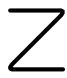
\includegraphics[keepaspectratio]{images/part001_11d71cd9.jpg}}

注. 1) 一个微分方程 (1) 在给定点处取同一值的积分可以有无穷多个。例如，数量微分方程 \(x' = 2\sqrt{|x|}\) 以由下列式子定义的诸函数

\[
\begin{array}{l l} u (t) = 0 & \text { for } \quad - \beta \leqslant t \leqslant \alpha \\ u (t) = - (t + \beta) ^ {2} & \text { for } \quad t \leqslant - \beta \\ u (t) = (t - \alpha) ^ {2} & \text { for } \quad t \geqslant \alpha \end{array}
\]

为其在点 t = 0 处取值 0 的积分，这里 \(\alpha\) 与 \(\beta\) 为任意正数。

\begin{enumerate}
\def\labelenumi{\arabic{enumi})}
\setcounter{enumi}{1}
\tightlist
\item
  当 \(\mathbf{E}\) 是任意无穷维的完备赋范空间时，佩亚诺定理不再成立（IV，第 204 页，习题 18）。
\end{enumerate}

\subsection{近似解的比较}

在下面，I 与 H 仍如前分别表示 R 中所包含的一个区间与赋范空间 E 中的一个开集；\(t_{0}\) 是 I 的一点。

定义 1. 给定定义在 I 上的正实函数 \(t \mapsto k(t)\)，称映射 \(\mathbf{f}\)（从 \(\mathrm{I} \times \mathrm{H}\) 到 E 中）关于函数 \(k(t)\) 是利普希茨的，如果对每个 \(\mathbf{x} \in \mathrm{H}\)，函数 \(t \mapsto \mathbf{f}(t, \mathbf{x})\) 在 I 上规则，并且对每个 \(t \in \mathrm{I}\) 与 H 中的每一对点 \(\mathbf{x}_1, \mathbf{x}_2\)，有（“利普希茨条件”）

\[
\left\| \mathbf {f} (t, \mathbf {x} _ {1}) - \mathbf {f} (t, \mathbf {x} _ {2}) \right\| \leqslant k (t) \left\| \mathbf {x} _ {1} - \mathbf {x} _ {2} \right\|.\tag{8}
\]

我们说 \(\mathbf{f}\) 在 \(\mathrm{I} \times \mathrm{H}\) 上（不加限定地说）是利普希茨的，如果它关于某个常数 \(k \geqslant 0\) 在该集合上是利普希茨的。显然，\(\mathrm{I} \times \mathrm{H}\) 上的利普希茨函数满足 IV 第 165 页引理 1 的假设（反之不真）；当 \(\mathbf{f}\) 在 \(\mathrm{I} \times \mathrm{H}\) 上是利普希茨的时，就称微分方程

\[
\mathbf {x} ^ {\prime} = \mathbf {f} (t, \mathbf {x})\tag{1}
\]

是利普希茨的（在 I × H 上）。

例. 当 E = R 且 H 是 R 中的一个区间时，若函数 \(f(t, x)\) 具有偏导数 \(f_{x}^{\prime}\)（II，第 74 页），在 I × H 的每一点 \((t, x)\) 处，且在 I × H 上 \(|f_{x}^{\prime}(t, x)| \leqslant k(t)\)，则由中值定理，条件 (8) 得到满足；我们以后将看到这个例子怎样推广到 E 为任意赋范空间的情形。

若 f 在 \(I \times H\) 上是利普希茨的，则对每个紧子区间 \(J \times S\) 与每个开球 \(J \subset I\)，f 在 \(S \subset H\) 上有界。于是可以应用命题 3（IV，第 166 页），它给出方程 (1) 的近似解的存在性。但我们还有下面的命题，它使我们可以比较两个近似解：

命题 5. 设 \(k(t)\) 是实规则函数且在 I 上 \(>0\)，并设 \(\mathbf{f}(t, \mathbf{x})\) 是已定义且关于 \(k(t)\) 在 \(\mathrm{I} \times \mathrm{H}\) 上为利普希茨的函数。若 \(\mathbf{u}\) 与 \(\mathbf{v}\) 是 (1) 的两个近似解，其精确度分别为 \(\varepsilon_1\) 与 \(\varepsilon_2\)，都定义在 I 上且取值于 H 中，则对每个 \(t \in \mathrm{I}\)（只要 \(t \geqslant t_0\)），

\[
\left\| \mathbf {u} (t) - \mathbf {v} (t) \right\| \leqslant \left\| \mathbf {u} \left(t _ {0}\right) - \mathbf {v} \left(t _ {0}\right) \right\| \Phi (t) + \left(\varepsilon_ {1} + \varepsilon_ {2}\right) \Psi (t)\tag{9}
\]

其中

\[
\left\{ \begin{array}{l} \Phi (t) = 1 + \int_ {t _ {0}} ^ {t} k (s) \exp \left(\int_ {s} ^ {t} k (\tau) d \tau\right) d s \\ \Psi (t) = t - t _ {0} + \int_ {t _ {0}} ^ {t} (s - t _ {0}) k (s) \exp \left(\int_ {s} ^ {t} k (\tau) d \tau\right) d s. \end{array} \right.\tag{10}
\]

由关系式 \(\left\| \mathbf{u}'(t) - \mathbf{f}(t, \mathbf{u}(t)) \right\| \leqslant \varepsilon_1\)（它在某个可数集的补集上成立），借助中值定理推出

\[
\left\| \mathbf {u} (t) - \mathbf {u} (t _ {0}) - \int_ {t _ {0}} ^ {t} \mathbf {f} (s, \mathbf {u} (s)) d s \right\| \leqslant \varepsilon_ {1} (t - t _ {0})
\]

同理可得

\[
\left\| \mathbf {v} (t) - \mathbf {v} (t _ {0}) - \int_ {t _ {0}} ^ {t} \mathbf {f} (s, \mathbf {v} (s)) d s \right\| \leqslant \varepsilon_ {2} (t - t _ {0})
\]

由此得

\[
\begin{array}{l} \| \mathbf {u} (t) - \mathbf {v} (t) \| \leqslant \| \mathbf {u} (t _ {0}) - \mathbf {v} (t _ {0}) \| \\ \qquad + \left\| \int_ {t _ {0}} ^ {t} (\mathbf {f} (s, \mathbf {u} (s)) - \mathbf {f} (s, \mathbf {v} (s))) d s \right\| + (\varepsilon_ {1} + \varepsilon_ {2}) (t - t _ {0}). \end{array}
\]

由利普希茨条件 (8) 有

\[
\begin{array}{r l} \left\| \int_ {t _ {0}} ^ {t} (\mathbf {f} (s, \mathbf {u} (s)) - \mathbf {f} (s, \mathbf {v} (s))) d s \right\| & \leqslant \int_ {t _ {0}} ^ {t} \| \mathbf {f} (s, \mathbf {u} (s)) - \mathbf {f} (s, \mathbf {v} (s)) \| d s \\ & \leqslant \int_ {t _ {0}} ^ {t} k (s) \| \mathbf {u} (s) - \mathbf {v} (s) \| d s \end{array}
\]

由此，令 \(w(t) = \|\mathbf{u}(t) - \mathbf{v}(t)\|\)，即得

\[
w (t) \leqslant w \left(t _ {0}\right) + \left(\varepsilon_ {1} + \varepsilon_ {2}\right) \left(t - t _ {0}\right) + \int_ {t _ {0}} ^ {t} k (s) w (s) d s.\tag{11}
\]

因此本命题是下述引理的推论：

引理 2. 若 \(w\) 是区间 \([t_0, t_1]\) 上的连续实函数且满足不等式

\[
w (t) \leqslant \varphi (t) + \int_ {t _ {0}} ^ {t} k (s) w (s) d s\tag{12}
\]

其中 \(\varphi\) 是规则函数 \(\geqslant 0\) 在 \([t_0, t_1]\) 上，则对 \(t_0 \leqslant t \leqslant t_1\)，

\[
w (t) \leqslant \varphi (t) + \int_ {t _ {0}} ^ {t} \varphi (s) k (s) \exp \left(\int_ {s} ^ {t} k (\tau) d \tau\right) d s.\tag{13}
\]

令 \(y(t) = \int_{t_0}^{t} k(s)w(s)ds\)；关系式 (12) 蕴含

\[
y ^ {\prime} (t) - k (t) y (t) \leqslant \varphi (t) k (t)\tag{14}
\]

在一个可数集的补集上。

令 \(z(t) = y(t)\exp \left(-\int_{t_0}^t k(s)ds\right)\)；则 (14) 等价于

\[
z ^ {\prime} (t) \leqslant \varphi (t) k (t) \exp \left(- \int_ {t _ {0}} ^ {t} k (s) d s\right).
\]

对此不等式应用中值定理（I，第 15 页，定理 2），并注意到 \(z(t_0) = 0\)，便得到

\[
z (t) \leqslant \int_ {t _ {0}} ^ {t} \varphi (s) k (s) \exp \left(- \int_ {t _ {0}} ^ {s} k (\tau) d \tau\right) d s
\]

由此得

\[
y (t) \leqslant \int_ {t _ {0}} ^ {t} \varphi (s) k (s) \exp \left(\int_ {s} ^ {t} k (\tau) d \tau\right) d s
\]

又因 \(w(t) \leqslant \varphi(t) + y(t)\)，这样就得到 (13)。

推论. 设 f 是关于常数 k \textgreater{} 0、定义在 I × H 上的利普希茨函数。若 u 与 v 是 (1) 的两个近似解，其精确度分别为 \(\varepsilon_{1}\) 与 \(\varepsilon_{2}\)，都定义在 I 上且取值于 H 中，则对一切 \(t \in I\)，

\[
\| \mathbf {u} (t) - \mathbf {v} (t) \| \leqslant \| \mathbf {u} (t _ {0}) - \mathbf {v} (t _ {0}) \| e ^ {k | t - t _ {0} |} + (\varepsilon_ {1} + \varepsilon_ {2}) \frac {e ^ {k | t - t _ {0} |} - 1}{k}.\tag{15}
\]

当 \(t \geqslant t_0\) 时，此不等式实际上是 (9) 的直接推论；要对 \(t \leqslant t_0\) 证明它，只需把它应用于方程

\[
{\frac {d \mathbf {x}}{d s}} = - \mathbf {f} (- s, \mathbf {x})
\]

它是通过变量代换 t = -s 从 (1) 得到的。

注. 1) 当 k = 0 时，不等式 (15) 换成不等式

\[
\left\| \mathbf {u} (t) - \mathbf {v} (t) \right\| \leqslant \left\| \mathbf {u} \left(t _ {0}\right) - \mathbf {v} \left(t _ {0}\right) \right\| + \left(\varepsilon_ {1} + \varepsilon_ {2}\right) | t - t _ {0} |
\]

其证明是直接的。

\begin{enumerate}
\def\labelenumi{\arabic{enumi})}
\setcounter{enumi}{1}
\tightlist
\item
  当 E 是有限维且 f 在 \(I \times H\) 上是利普希茨的时候，可以不用选择公理（IV，第 199 页，习题 1 b)）来证明 (1) 的近似解的存在性（IV，第 166 页，命题 3）。
\end{enumerate}

命题 6. 设 f 与 g 是定义在 I × H 上的两个函数，它们满足 IV 第 165 页引理 1 的假设，并且在 I × H 上

\[
\left\| \mathbf {f} (t, \mathbf {x}) - \mathbf {g} (t, \mathbf {x}) \right\| \leqslant \alpha .\tag{16}
\]

再设 \(\mathbf{g}\) 是关于常数 \(k > 0\) 在 \(\mathrm{I} \times \mathrm{H}\) 上为利普希茨的函数。在这些条件下，若 \(\mathbf{u}\) 是 \(\mathbf{x}' = \mathbf{f}(t, \mathbf{x})\) 的精确到 \(\varepsilon_1\) 的近似解，它定义在 \(\mathrm{I}\) 上、取值于 \(\mathrm{H}\) 中，而 \(\mathbf{v}\) 是 \(\mathbf{x}' = \mathbf{g}(t, \mathbf{x})\) 的精确到 \(\varepsilon_2\) 的近似解，它定义在 \(\mathrm{I}\) 上、取值于 \(\mathrm{H}\) 中，则对一切 \(t \in \mathrm{I}\)

\[
\| \mathbf {u} (t) - \mathbf {v} (t) \| \leqslant \| \mathbf {u} (t _ {0}) - \mathbf {v} (t _ {0}) \| e ^ {k | t - t _ {0} |} + (\alpha + \varepsilon_ {1} + \varepsilon_ {2}) \frac {e ^ {k | t - t _ {0} |} - 1}{k}.\tag{17}
\]

的确

\[
\left| \left| \mathbf {u} ^ {\prime} (t) - \mathbf {g} (t, \mathbf {u} (t)) \right| \right| \leqslant \alpha + \varepsilon_ {1}
\]

此式对 I 中某个可数子集在 I 中的补集的所有 t 成立；换言之，u 是 \(\mathbf{x}^{\prime} = \mathbf{g}(t, \mathbf{x})\) 的精确到 \(\alpha + \varepsilon_{1}\) 的近似解，于是应用 IV 第 169 页的命题 5 即得不等式 (17)。

\subsection{利普希茨方程与局部利普希茨方程的解的存在性与唯一性}

定理 1（柯西）. 设 \(\mathbf{f}\) 是 \(\mathrm{I} \times \mathrm{H}\) 上的利普希茨函数，设 \(\mathrm{J}\) 是 \(\mathrm{I}\) 的一个不退化为一点的紧子区间，\(t_0\) 是 \(\mathrm{J}\) 的一点，\(\mathrm{S}\) 是以 \(\mathbf{x}_0\) 为中心、以 \(r\) 为半径、包含于 \(\mathrm{H}\) 中的开球，而 \(\mathrm{M}\) 是 \(\| \mathbf{f}(t, \mathbf{x})\|\) 在 \(\mathrm{J} \times \mathrm{S}\) 上的上确界。在这些条件下，对每个紧区间 \(\mathrm{K}\)，若它不退化为一点、包含于 \(\mathrm{J}\) 与 \(]t_0 - r / M\)、\(t_0 + r / M[\) 的交中且包含 \(t_0\)，则存在微分方程 \(\mathbf{x}' = \mathbf{f}(t, \mathbf{x})\) 的唯一一个解，它定义在 \(\mathrm{K}\) 上、取值于 \(\mathrm{S}\) 中、且在点 \(\mathbf{x}_0\) 处等于 \(t_0\) 。

的确，当 \(\varepsilon > 0\) 足够小时，\(F_{\varepsilon}\)（即 (1) 的精确到 \(\varepsilon\) 、定义在 K 上、取值于 S 中且等于 \(x_{0}\) 于点 \(t_{0}\) 的近似解）非空（IV，第 166 页，命题 3）；此外，若 u 与 v 都属于 \(F_{\varepsilon}\) ，则由 (15)（IV，第 170 页）

\[
\| \mathbf {u} (t) - \mathbf {v} (t) \| \leqslant 2 \varepsilon \frac {e ^ {k | t - t _ {0} |} - 1}{k}
\]

对一切 \(t \in K\) ，于是诸集 \(F_{\varepsilon}\) 构成一个滤基 G，它在 K 上一致收敛于一个连续函数 w，后者等于 \(x_{0}\) 于 \(t_{0}\) ；而且 w 取值于 S 中，因为当 \(\varepsilon\) 足够小时，诸函数 \(u \in F_{\varepsilon}\) 的值都属于一个包含于 S 中的闭球。由于 \(\mathbf{f}(t, \mathbf{u}(t))\) 沿 G 在 K 上一致趋于 \(\mathbf{f}(t, \mathbf{w}(t))\) ，w 满足 IV 第 165 页的方程 (6)，因而是 (1) 的解。解的唯一性由 IV 第 170 页的不等式 (15) 立即得出，其中取 \(\varepsilon_{1} = \varepsilon_{2} = 0\) 与 \(\mathbf{u}(t_{0}) = \mathbf{v}(t_{0})\) 。

我们说函数 \(\mathbf{f}\)（定义在 \(\mathrm{I} \times \mathrm{H}\) 上）是局部利普希茨的，如果对 \((t, \mathbf{x})\) 的每个点 \(\mathrm{I} \times \mathrm{H}\) ，存在 \(\mathrm{V}\) 的一个邻域 \(t\)（关于 \(\mathrm{I}\) ）与 \(\mathrm{S}\) 的一个邻域 \(\mathbf{x}\)，使得 \(\mathbf{f}\) 在 \(\mathrm{V} \times \mathrm{S}\) 上是利普希茨的（常数 \(k\) 依赖于 \(\mathrm{V}\) 与 \(\mathrm{S}\) ）。由博雷尔–勒贝格定理，对每个紧区间 \(\mathrm{J} \subset \mathrm{I}\) 与每个点 \(\mathbf{x}_0 \in \mathrm{H}\)，存在以 \(\mathrm{S}\) 为中心、包含于 \(\mathbf{x}_0\) 中的开球 \(\mathrm{H}\)，使得 \(\mathbf{f}\) 在 \(\mathrm{J} \times \mathrm{S}\) 上是利普希茨的；于是 \(\mathbf{f}\) 满足 IV 第 3 页引理 1 的假设。当 \(\mathbf{f}\) 在 \(\mathrm{I} \times \mathrm{H}\) 上是局部利普希茨的时候，我们称方程 \(\mathbf{x}' = \mathbf{f}(t, \mathbf{x})\) 在 \(\mathrm{I} \times \mathrm{H}\) 上是局部利普希茨的。

我们要对局部利普希茨方程推广并阐明 IV 第 10 页的定理 1；我们限于 \(t_0\) 是区间 I 的左端点的情形；对 \(t_0\) 是 I 的任意点的情形，容易化归为上述情形（参看 IV，§ IV ??，第 9 页，推论）。

定理 2. 设 \(\mathbf{I} \subset \mathbf{R}\) 是一个（不退化为一点的）区间，其左端点为 \(t_0 \in \mathbf{I}\) ；设 \(\mathbf{H}\) 是 \(\mathbf{E}\) 中的一个非空开集，并设 \(\mathbf{f}\) 是 \(\mathbf{I} \times \mathbf{H}\) 上的局部利普希茨函数。

\(1^{\circ}\) 对 \(\mathbf{x}_0\in \mathrm{H}\) ，存在最大的区间 \(\mathbf{J}\subset \mathbf{I}\)（其左端点为 \(t_0\in \mathbf{J}\) ），在该区间上存在一个积分 \(\mathbf{u}\) ，即方程 \(\mathbf{x}' = \mathbf{f}(t,\mathbf{x})\) 的、取值于 H 中且等于 \(\mathbf{x}_0\) 于点 \(t_0\) 的积分；这个积分是唯一的。

\(2^{\circ}\) 若 \(\mathrm{J} \neq \mathrm{I}\) ，则 \(\mathrm{J}\) 是长度有限的半开区间 \([t_0, \beta[\) ；此外，对每个紧子集 \(\mathbf{K} \subset \mathbf{H}\) ，集合 \(\overline{\mathbf{u}}^{-1}(\mathbf{K})\) 是 \(\mathbf{R}\) 的紧子集。

\(3^{\circ}\) 若 \(\mathbf{J}\) 有界，且若 \(\mathbf{f}(t,\mathbf{u}(t))\) 在 \(\mathbf{J}\) 上有界，则 \(\mathbf{u}(t)\) 在 \(\mathbf{c}\) 的右端点处有左极限 \(\mathbf{J}\) ；此外，若 \(\mathbf{J} \neq \mathbf{I}\) ，则 \(\mathbf{c}\) 是 \(\mathbf{H}\) 在 \(\mathbf{E}\) 中的边界点。

\(1^{\circ}\) 设 \(\mathfrak{M}\) 是由这样的区间 L（不退化为一点、左端点为 \(t_0 \in L\) 、包含于 I）组成的集合：在 L 上存在 (1)（IV，第 163 页）的、取值于 H 中且等于 \(\mathbf{x}_0\) 于 \(t_0\) 的解；由定理 1（IV，第 171 页），集合 \(\mathfrak{M}\) 非空。设 L 与 L' 是属于 \(\mathfrak{M}\) 的两个区间，例如设 L \(\subset\) L'；若 u 与 v 是 (1) 的两个积分，分别定义在 L 与 L' 上、取值于 H 中且等于 \(\mathbf{x}_0\) 于 \(t_0\) ，我们将看到 v 是 u 的扩张。的确，设 \(t_1\) 是使 \(t \in L\) 满足 \(\mathbf{u}(s) = \mathbf{v}(s)\) （对 \(t_0 \leqslant s \leqslant t\) ）的 t 组成的集合的上确界；我们将证明 \(t_1\) 是 L 的右端点。若非如此，则由连续性有 \(\mathbf{u}(t_1) = \mathbf{v}(t_1)\) ，且 \(\mathbf{x}_1 = \mathbf{u}(t_1)\) 属于 H；由于 f 是局部利普希茨的，定理 1 表明只能存在 (1) 的一个在 \(t_1\) 的邻域上定义、取值于 H 中且等于 \(\mathbf{x}_1\) 于 \(t_1\) 的积分；因此假定 \(t_1\) 不是 L 的右端点便导致矛盾。现在我们看到，若 J 是诸区间 L \(\in\) M 的并，则存在 (1) 的唯一一个积分 u，它定义在 J 上、取值于 H 中且等于 \(\mathbf{x}_0\) 于 \(t_0\) 。

\(2^{\circ}\) 设 \(\mathrm{J} \neq \mathrm{I}\) ，并设 \(\beta\) 是 \(\mathrm{J}\) 的右端点；若 \(\beta\) 是 \(\mathrm{I}\) 的右端点，则 \(\beta \in \mathrm{I}\) （于是 \(\beta\) 是有限的），且由假设 \(\mathrm{J} = [t_0, \beta[\) 。今设 \(\beta\) 不是 \(\mathrm{I}\) 的右端点；若 \(\beta \in \mathrm{J}\) ，则 \(\mathbf{u}(\beta) = \mathbf{c}\) 属于 \(\mathrm{H}\) ；由定理 1，存在 (1) 的一个取值于 \(\mathrm{H}\) 中、定义在一个区间上的积分

\[
[ \beta , \beta_ {1} [ \subset I
\]

且等于 \(\mathbf{c}\) 于 \(\beta\) ；这样 \(\mathrm{J}\) 就不是 \(\mathfrak{M}\) 中最大的区间，这是荒谬的；故 \(\mathrm{J} = [t_0, \beta[\) 。

若 K 是 H 的紧子集，则 \(\overline{\mathbf{u}}^{-1}(\mathbf{K})\) 在 J 中是闭的；我们将看到存在 \(\gamma\in J\) 使得 \(\overline{\mathbf{u}}^{-1}(\mathbf{K})\) 包含于 \([t_{0},\gamma]\) 中，这就证明 \(\overline{\mathbf{u}}^{-1}(\mathbf{K})\) 是紧的。若不然，就会存在一点 \(c\in K\) 使得 \((\beta,\mathbf{c})\) 是点 \((t,\mathbf{u}(t))\)（其中 \(t<\beta\) 与 \(\mathbf{u}(t)\in\mathbf{K}\) ）所成之集的聚点。由于 \(\beta\in I\) 与 \(c\in H\) ，则存在 \(\beta\) 在 I 中的邻域 V，以及以 c 为中心、半径 r 且包含于 H 中的开球 S，使得 f 在 V×S 上是利普希茨的且有界；令 M 为 \(\|\mathbf{f}(t,\mathbf{x})\|\) 在该集合上的上确界。由假设存在 \(t_{1}\in J\) 使得 \(\beta-t_{1}<r/2M\) 、\(t_{1}\in V\) 与 \(\|\mathbf{u}(t_{1})-\mathbf{c}\|\leqslant r/2\) ；定理 1 表明存在 (1) 的唯一一个积分，它取值于 H 中、定义在包含 \([t_{1},t_{2}]\) 的区间 \(\beta\) 上、且等于 \(\mathbf{u}(t_{1})\) 于 \(t_{1}\) ；由于这个区间在区间 \([t_{1},\beta[\) 上与 u 一致，便推出 \(J=[t_{0},\beta[\) 不是 M 中最大的区间，这是荒谬的。

\(3^{\circ}\) 设 \(\mathbf{J}\) 有界且 \(\| \mathbf{f}(t,\mathbf{u}(t))\| \leqslant M\) 在 \(\mathbf{J}\) 上成立；则在 \(\| \mathbf{u}'(t)\| \leqslant \mathbf{M}\) 于 \(\mathbf{J}\) 的一个可数子集的补集上成立；于是由中值定理，对 \(\| \mathbf{u}(s) - \mathbf{u}(t)\| \leqslant \mathbf{M} |s - t|\) 与 \(s\)（都属于 \(t\) ）有 \(\mathbf{J}\) ；由柯西准则，\(\mathbf{u}\) 有左极限 \(\mathbf{c}\) 于 \(\beta\) 处（它是 \(\mathbf{J}\) 的右端点）；若 \(\mathbf{J} \neq \mathbf{I}\) ，则 \(\mathbf{c}\) 不可能属于 \(\mathbf{H}\) ，因为把 \(\mathbf{u}\) 在 \(\beta\) 处连续延拓后，\(\mathbf{u}\) 就成为 (1) 的一个取值于 \(\mathbf{H}\) 中、定义在区间 \([t_0, \beta]\) 上且等于 \(\mathbf{x}_0\) 于 \(t_0\) 的积分；于是就有 \(\mathbf{J} = [t_0, \beta]\) ，这与我们在 \(2^{\circ}\) 中已看到的相矛盾。

推论 1. 若 H = E 且 J ≠ I，则 \(\mathbf{f}(t, \mathbf{u}(t))\) 在 J 上不是有界的；进而，若 E 是有限维的，则 \(\| \mathbf{u}(t) \|\) 在 J 的右端点处有左极限 \(+\infty\) 。

第一部分是定理 2 第三部分的直接推论。若 E 是有限维的，则每个闭球 \(S \subset E\) 是紧的，于是定理 2 的第二部分表明存在 \(\gamma \in J\) 使得 \(\mathbf{u}(t) \notin \mathbf{S}\) 对 \(t > \gamma\) 成立。

若 E 是有限维的，可能发生这样的情况：\(J \neq I\) 而 \(\|\mathbf{u}(t)\|\) 当 t 趋于 J 的右端点时保持有界（IV，第 200 页，习题 5）。

推论 2. 若在 I × H 上函数 f 关于一个规则函数 k(t) 是利普希茨的，且若 J 的右端点 β 属于 I，则 u 在 β 处有左极限；若 H = E 且 f 在 I × E 上关于一个规则函数 k(t) 是利普希茨的，则 J = I。

的确，若 \(\beta \in \mathbf{I}\) ，则存在 \(\mathrm{V}\) 在 \(\beta\) 中的一个紧邻域 \(\mathbf{I}\) ，使得 \(\mathbf{f}(t, \mathbf{x}_0)\) 与 \(k(t)\) 在 \(\mathrm{V}\) 上有界；于是 \(\| \mathbf{f}(t, \mathbf{x}) \| \leqslant m \| x \| + h\) （\(m\) 与 \(h\) 为常数）

在 \(V \times H\) 上成立，由此 \(\left\|\mathbf{u}^{\prime}(t)\right\| \leqslant m \left\|\mathbf{u}(t)\right\| + h\) 在 \(V \cap J\) 的一个可数子集的补集上成立，从而 \(\left\|\mathbf{u}(t)\right\| \leqslant m \int_{t_{0}}^{t} \left\|\mathbf{u}(s)\right\| ds + q\) （q 为常数）在 \(V \cap J\) 上成立；引理 2（IV，第 170 页）表明 \(\left\|\mathbf{u}(t)\right\| \leqslant c e^{mt} + d\) （c 与 d 为常数）在 \(V \cap J\) 上成立，于是 \(\mathbf{f}(t, \mathbf{u}(t))\) 在 J 上保持有界，从而由 IV 第 172 页的定理 2 即得本推论。

例. 1) 对形如 \(\mathbf{x}' = \mathbf{g}(t)\) 的微分方程（其中 \(\mathbf{g}\) 在 I 上是规则的），每个积分 \(\mathbf{u}\) 显然都定义在整个 I 上。应当注意，\(\mathbf{u}\) 可以在 I 上有界而 \(\mathbf{g}(t)\) 并不如此。

\begin{enumerate}
\def\labelenumi{\arabic{enumi})}
\setcounter{enumi}{1}
\item
  对数量方程 \(x' = \sqrt{1 - x^2}\) 有 \(I = R\) ，\(H = ] - 1, +1[\) 。若取 \(t_0 = x_0 = 0\) ，则相应的积分是 \(\sin t\) ，其定义区间是包含 0 且使 \(\sin t\) 的导数为正的最大区间，也就是说，\(] - \pi / 2, +\pi / 2[\) ；在这个区间的端点处，积分趋于 \(H\) 的一个端点。
\item
  对数量方程 \(x' = 1 + x^{2}\) 有 I = H = R；在 t = 0 处为零的积分是 \(\tan t\) ，而包含 0 且使该函数连续的最大区间是 \(J = ] - \pi/2, +\pi/2[\) ；且 \(|\tan t|\) 在 J 的端点处趋于 \(+\infty\) （参看 IV，第 173 页，推论 1）。
\item
  对数量方程 \(x' = \sin tx\) 有 I = H = R，且右端在 I × H 上有界，故（IV，第 173 页，推论 1）每个积分都定义在整个 R 上。
\end{enumerate}

\subsection{积分作为参数函数的连续性}

命题 6（IV，第 171 页）表明：当一个微分方程

\[
\mathbf {x} ^ {\prime} = \mathbf {f} (t, \mathbf {x})
\]

“接近”于一个利普希茨方程 \(\mathbf{x}^{\prime} = \mathbf{g}(t, \mathbf{x})\) ，且当假定两个方程在同一区间上都有近似解时，这两个近似解是“接近”的；我们将阐明这个结果，办法是证明：只要利普希茨方程 \(\mathbf{x}^{\prime} = \mathbf{g}(t, \mathbf{x})\) 在某区间上存在解，便蕴含方程 \(\mathbf{x}^{\prime} = \mathbf{f}(t, \mathbf{x})\) 在同一区间上近似解的存在，前提是在该区间上，方程 \(\mathbf{x}^{\prime} = \mathbf{g}(t, \mathbf{x})\) 的解的值并不“太接近” H 的边界。

命题 7. 设 f 与 g 是定义在 I × H 上的两个函数，满足 IV 第 165 页引理 1 的假设，并且在 I × H 上

\[
\left\| \mathbf {f} (t, \mathbf {x}) - \mathbf {g} (t, \mathbf {x}) \right\| \leqslant \alpha .\tag{16}
\]

再设 \(\mathbf{g}\) 关于常数 \(k > 0\) 在 \(\mathrm{I} \times \mathrm{H}\) 上是利普希茨的，且 \(\mathbf{f}\) 在 \(\mathrm{I} \times \mathrm{H}\) 上是局部利普希茨的，或者 \(\mathrm{E}\) 是有限维的。设 \((t_0, \mathbf{x}_0)\) 是 \(\mathrm{I} \times \mathrm{H}\) 的一点，\(\mu\) 是一个数 \(>0\) ，并设

\[
\varphi (t) = \mu e ^ {k (t - t _ {0})} + \alpha \frac {e ^ {k (t - t _ {0})} - 1}{k}.
\]

设 \(\mathbf{u}\) 是方程 \(\mathbf{x}' = \mathbf{g}(t, \mathbf{x})\) 的一个积分，它定义在包含于 I 的区间 \(\mathrm{K} = [t_0, b[\) 上、等于 \(\mathbf{x}_0\) 于点 \(t_0\) ，并且对一切 \(t \in \mathrm{K}\) ，以 \(\mathbf{u}(t)\) 为中心、以 \(\varphi(t)\) 为半径的闭球都包含于 H 中。在这些条件下，对每个满足 \(\mathbf{y} \in \mathrm{H}\) 的 \(\| \mathbf{y} - \mathbf{x}_0 \| \leqslant \mu\) ，便存在 \(\mathbf{v}\) ，它是方程 \(\mathbf{x}' = \mathbf{f}(t, \mathbf{x})\) 的一个积分，定义在 K 上、取值于 H 中且等于 \(\mathbf{y}\) 于点 \(t_0\) ；此外，在 K 上有 \(\| \mathbf{u}(t) - \mathbf{v}(t) \| \leqslant \varphi(t)\) 。

设 M 是 \(\mathbf{x}^{\prime} = \mathbf{f}(t, \mathbf{x})\) 的积分所成的族，其中每个积分都取值于 H 中、在 \(t_{0}\) 处等于 y、且定义在一个包含于 I 的半开区间 \([t_{0}, \tau[\) 上（该区间随所考虑的积分而异）。由 IV 第 171 页的定理 1（当 f 是局部利普希茨时）或 IV 第 167 页的推论（当 E 是有限维时），M 非空，且与 IV 第 166 页命题 3 中同样的推理表明，M 依序关系“v 是 w 的限制”是归纳的。设 \(v_{0}\) 是 M 的一个极大元，\([t_{0}, t_{1}[\) 是 \(v_{0}\) 的定义区间；由 IV 第 171 页的命题 6，一切都归结为证明 \(t_{1} \geqslant b\) 。若不然，则有

\[
\left\| \mathbf {u} (t) - \mathbf {v} _ {0} (t) \right\| \leqslant \varphi (t)
\]

在区间 \([t_0, t_1[\) 上此式由命题 6 得出；而在紧区间 \([t_0, t_1]\) 上，规则函数 \(\mathbf{g}(t, \mathbf{u}(t))\) 有界，故函数 \(\mathbf{g}(t, \mathbf{v}_0(t))\) 在区间 \([t_0, t_1[\) 上有界，因为在此区间上 \(\| \mathbf{g}(t, \mathbf{v}_0(t)) \| \leqslant \| \mathbf{g}(t, \mathbf{u}(t)) \| + k\varphi(t)\) 。由于 \(\mathbf{v}_0\) 是 \(\mathbf{x}' = \mathbf{g}(t, \mathbf{x})\) 的精确到 \(\alpha\) 的近似解（在 \([t_0, t_1[\) 上），故存在数 \(M > 0\) 使得在此区间上除去一个可数集的点以外有 \(\| \mathbf{v}_0'(t) \| \leqslant M\) ；于是中值定理表明 \(\| \mathbf{v}_0(s) - \mathbf{v}_0(t) \| \leqslant M |s - t|\) ，对每对点 \(s\) 与 \(t\)（都属于 \([t_0, t_1[\) ）成立，从而（由柯西准则）\(\mathbf{v}_0(t)\) 有左极限 \(\mathbf{c}\) 于点 \(t_1\) ，并且由连续性有 \(\| \mathbf{c} - \mathbf{u}(t_1) \| \leqslant \varphi(t_1)\) ，故 \(\mathbf{c} \in H\) 。于是由 IV 第 171 页定理 1 或 IV 第 167 页推论可见，存在 \(\mathbf{x}' = \mathbf{f}(t, \mathbf{x})\) 的一个积分，它定义在区间 \([t_1, t_2[\) 上且等于 \(\mathbf{c}\) 于 \(t_1\) ，这与 \(\mathbf{v}_0\) 的定义相矛盾。

定理 3. 设 F 是一个拓扑空间，f 是从 I × H × F 到 E 中的一个映射，使得对每个 \(\xi \in F\) ，函数 \((t, \mathbf{x}) \mapsto \mathbf{f}(t, \mathbf{x}, \xi)\) 在 I × H 上是利普希茨的，并且当 \(\xi\) 趋于 \(\xi_{0}\) 时，\(\mathbf{f}(t, \mathbf{x}, \xi)\) 在 I × H 上一致趋于 \(\mathbf{f}(t, \mathbf{x}, \xi_{0})\) 。设 \(\mathbf{u}_{0}(t)\) 是 \(\mathbf{x}' = \mathbf{f}(t, \mathbf{x}, \xi_{0})\) 的一个积分，它定义在包含于 I 中的区间 J = {[}t₀, b{[} 上、取值于 H 中且在 t₀ 处等于 \(x_{0}\) 。对每个包含于 J 中的紧区间 {[}t₀, t₁{]} ，存在 \(\xi_{0}\) 在 F 中的一个邻域 V，使得对每个 \(\xi \in V\) ，方程 \(\mathbf{x}' = \mathbf{f}(t, \mathbf{x}, \xi)\) 有一个（且仅有一个）积分 \(\mathbf{u}(t, \xi)\) ，它定义在 {[}t₀, t₁{]} 上、取值于 H 中且在 t₀ 处等于 \(x_{0}\) ；而且，当 \(\xi\) 趋于 \(\xi_{0}\) 时，解 \(\mathbf{u}(t, \xi)\) 在 \(\mathbf{u}_{0}(t)\)[{t₀, t₁}]{ 上一致趋于 } 。

的确，取 r \textgreater{} 0，使得对 \(t_{0} \leqslant t \leqslant t_{1}\) ，以 \(\mathbf{u}_{0}(t)\) 为中心、以 r 为半径的闭球包含于 H 中；若 \(\mathbf{f}(t, \mathbf{x}, \xi)\) 关于常数 k \textgreater{} 0 在 I × H 上是利普希茨的，则取 \(\alpha\) 足够小，使 \(\alpha \frac{e^{k(t_{1}-t_{0})} - 1}{k} < r\) ；取 V 使得对每个 \(\xi \in V\) ，在 I × H 上有 \(\|f(t, \mathbf{x}, \xi) - f(t, \mathbf{x}, \xi_{0})\| \leqslant \alpha\) ，就可以应用 IV 第 174 页的命题 7；此外，

\[
\| \mathbf {u} (t, \xi) - \mathbf {u} _ {0} (t) \| \leqslant \alpha \frac {e ^ {k \left(t _ {1} - t _ {0}\right)} - 1}{k}
\]

在 \([t_{0}, t_{1}]\) 上，这就完成了定理的证明。

注. 当 H = E 且 IV 第 174 页的条件 (16) 在 I × E 上满足时，IV 第 174 页的命题 7 可应用于 \(\mathbf{x}' = \mathbf{g}(t, \mathbf{x})\) 的每个解 u，在其有定义的任何区间上；甚至还可以假定 \(\mathbf{g}(t,\mathbf{x})\) 关于一个规则函数 \(k(t)\) 是利普希茨的，尽管该函数在此区间上未必有界。

\subsection{对初始条件的依赖性}

设 \(\mathbf{x}^{\prime}=\mathbf{f}(t,\mathbf{x})\) 是 \(I\times H\) 上的局部利普希茨方程；由定理 2（IV，第 172 页），对 \((t_{0},\mathbf{x}_{0})\) 的每个点 \(I\times H\) ，存在最大的区间 \(J(t_{0},\mathbf{x}_{0})\subset I\) （不退化为一点、包含 \(t_{0}\) ），在该区间上存在此方程的一个（且仅有的一个）积分，它等于 \(x_{0}\) 于 \(t_{0}\) ；我们将阐明这个积分以及其定义区间 \(J(t_{0},\mathbf{x}_{0})\) 依赖点 \((t_{0},\mathbf{x}_{0})\) 的方式。

定理 4. 设 \(\mathbf{f}\) 是 \(\mathrm{I} \times \mathrm{H}\) 上的局部利普希茨函数，而 \((a, \mathbf{b})\) 是 \(\mathrm{I} \times \mathrm{H}\) 的任意一点。

\(1^{\circ}\) 存在一个区间 \(\mathbf{K} \subset \mathbf{I}\) （即 \(a\) 在 \(\mathbf{I}\) 中的邻域）和一个 \(\mathbf{V}\) 在 \(\mathbf{b}\) 中的邻域 \(\mathbf{H}\) ，使得对 \((t_0, \mathbf{x}_0)\) 的每个点 \(\mathbf{K} \times \mathbf{V}\) ，存在一个（且仅有一个）积分 \(\mathbf{u}(t, t_0, \mathbf{x}_0)\) ，它定义在 \(\mathbf{K}\) 上、取值于 \(\mathbf{H}\) 中且等于 \(\mathbf{x}_0\) 于点 \(t_0\) （换言之，\(J(t_0, \mathbf{x}_0) \supset \mathbf{K}\) 对一切 \((t_0, \mathbf{x}_0) \in \mathbf{K} \times \mathbf{V}\) 成立）。

\(2^{\circ}\) 映射 \((t,t_0,\mathbf{x}_0)\mapsto \mathbf{u}(t,t_0,\mathbf{x}_0)\)（从 \(\mathrm{K}\times \mathrm{K}\times \mathrm{V}\) 到 H 中）是一致连续的。

\(3^{\circ}\) 存在 \(\mathbf{W} \subset \mathbf{V}\) 在 \(\mathbf{b}\) 中的一个邻域 \(\mathbf{H}\) ，使得对每个点

\[
(t, t _ {0}, \mathbf {x} _ {0}) \in \mathrm{K} \times \mathrm{K} \times \mathrm{W},
\]

方程 \(\mathbf{x}_{0} = \mathbf{u}(t_{0}, t, \mathbf{x})\) 在 V 上有唯一的解 x，它等于 \(\mathbf{u}(t, t_{0}, \mathbf{x}_{0})\)（“把积分关于积分常数解出”）。

\(1^{\circ}\) 设 S 是以 \(\mathbf{b}\) 为中心、以 \(r\) 为半径且包含于 H 中的球，并设 \(\mathrm{J}_0\) 是包含于 I 的区间，即 \(a\) 在 I 中的邻域，使得 \(\mathbf{f}\) 有界且是利普希茨的（关于某个常数 \(k\) ）于 \(\mathrm{J}_0 \times \mathrm{S}\) 上；用 M 表示 \(\| \mathbf{f}(t, \mathbf{x})\|\) 在 \(\mathrm{J}_0 \times \mathrm{S}\) 上的上确界。于是存在（IV，第 171 页，定理 1）一个区间 \(\mathrm{J} \subset \mathrm{J}_0\) （即 \(a\) 在 I 中的邻域）和一个积分 \(\mathbf{v}\) ，即方程 \(\mathbf{x}' = \mathbf{f}(t, \mathbf{x})\) 的一个积分，它定义在 J 上、取值于 S 中且等于 \(\mathbf{b}\) 于 \(a\) 。我们将看到，以 \(\mathbf{b}\) 为中心、以 \(r/2\) 为半径的开球 V，以及 J 与区间 \([a - l, a + l[\) （其中 \(l\) 足够小）的交 K，都合乎要求。的确，IV 第 174 页的命题 7（应用于集合 \(\mathrm{J}_0 \times \mathrm{S}\) 和 \(\alpha = 0\) 的情形）表明存在 \(\mathbf{x}' = \mathbf{f}(t, \mathbf{x})\) 的一个积分，它定义在 K 上、取值于 S 中且等于 \(\mathbf{x}_0\) 于一点 \(t_0 \in \mathrm{K}\) ，其条件是

\[
\left\| \mathbf {v} (t) - \mathbf {b} \right\| + \left\| \mathbf {v} (t _ {0}) - \mathbf {x} _ {0} \right\| e ^ {k | t - t _ {0} |} <   r\tag{18}
\]

对每个 \(t \in \mathbf{K}\) 。于是由中值定理有

\[
\| \mathbf {v} (t) - \mathbf {b} \| \leqslant \mathrm{M} | t - a | \leqslant \mathrm{M} l
\]

对每个 \(t \in \mathbf{K}\) ；由于 \(\| \mathbf{x}_0 - \mathbf{b} \| < r / 2\) ，可见只需取 \(l\) 使得

\[
\mathbf {M} l + (\mathbf {M} l + r / 2) e ^ {2 k l} <   r\tag{19}
\]

便可使关系式 (18) 对每个 \((t, t_{0}, \mathbf{x}_{0})\)（属于 \(K \times K \times V\) ）都成立。

\(2^{\circ}\) 由中值定理有

\[
\left\| \mathbf {u} (t _ {1}, t _ {0}, \mathbf {x} _ {0}) - \mathbf {u} (t _ {2}, t _ {0}, \mathbf {x} _ {0}) \right\| \leqslant \mathrm{M} \left| t _ {2} - t _ {1} \right|\tag{20}
\]

对 K 中的一切 \(t_0, t_1, t_2\) 与 V 中的 \(\mathbf{x}_0\) 。现在命题 5（IV，第 169 页）表明

\[
\left\| \mathbf {u} (t, t _ {0}, \mathbf {x} _ {1}) - \mathbf {u} (t, t _ {0}, \mathbf {x} _ {2}) \right\| \leqslant e ^ {2 k t} \left\| \mathbf {x} _ {2} - \mathbf {x} _ {1} \right\|\tag{21}
\]

对 K 中的每个 t 和 \(t_{0}\)，以及 V 中的 \(x_{1}\) 与 \(x_{2}\)。最后，若 \(t_{1}\) 与 \(t_{2}\) 是 K 中任意两点，

\[
\left\| \mathbf {u} \left(t _ {1}, t _ {2}, \mathbf {x} _ {0}\right) - \mathbf {u} \left(t _ {2}, t _ {2}, \mathbf {x} _ {0}\right) \right\| \leqslant \mathrm{M} \left| t _ {2} - t _ {1} \right|
\]

这是由中值定理得到的，也就是说

\[
\left\| \mathbf {u} (t _ {1}, t _ {2}, \mathbf {x} _ {0}) - \mathbf {x} _ {0} \right\| \leqslant \mathbf {M} \left| t _ {2} - t _ {1} \right|;
\]

由于 \(\mathbf{u}(t, t_2, \mathbf{x}_0)\) 与取值 \(\mathbf{u}(t_1, t_2, \mathbf{x}_0)\) 于点 \(t_1\) 的积分相同，命题 5（IV，第 169 页）表明

\[
\left\| \mathbf {u} (t, t _ {1}, \mathbf {x} _ {0}) - \mathbf {u} (t, t _ {2}, \mathbf {x} _ {0}) \right\| \leqslant \mathrm{Me} ^ {2 k l} | t _ {2} - t _ {1} |\tag{22}
\]

对 \(t, t_{1}, t_{2}\) 中的一切 \(\mathbf{K}\) 与 \(\mathbf{x}_{0}\) 中的一切 \(\mathrm{V}\) 都成立。于是三个不等式 (20)、(21) 与 (22) 证明了映射 \((t, t_{0}, \mathbf{x}_{0}) \mapsto \mathbf{u}(t, t_{0}, \mathbf{x}_{0})\) 在 \(\mathrm{K} \times \mathrm{K} \times \mathrm{V}\) 上的一致连续性。

\(3^{\circ}\) 由 (20)，有 \(\|\mathbf{u}(t, t_{0}, \mathbf{x}_{0}) - \mathbf{x}_{0}\| \leqslant \mathbf{M} |t - t_{0}| \leqslant 2\mathbf{M}l\) 于

\[
\mathbf {K} \times \mathbf {K} \times \mathbf {V}.
\]

若把 \(l\) 取得足够小，使 \(2\mathrm{M}l < r / 4\) ，则可以看出：若 \(\mathbf{x}_0\) 是以 \(\mathbf{W}\) 为中心、以 \(\mathbf{b}\) 为半径的开球 \(r / 4\) 中的任意一点，那么 \(\mathbf{u}(t,t_0,\mathbf{x}_0)\in \mathbf{V}\) 对任何 \(t\) 与 \(t_0\)（都属于 \(\mathbf{K}\) ）成立。若 \(\mathbf{x} = \mathbf{u}(t,t_0,\mathbf{x}_0)\) ，则函数 \(s\mapsto \mathbf{u}(s,t,\mathbf{x})\) 便定义在 \(\mathbf{K}\) 上，并且等于 (1) 的取值 \(\mathbf{x}\) 于点 \(t\) 的那个积分，也就是等于 \(\mathbf{u}(s,t_0,\mathbf{x}_0)\) ；特别地

\[
\mathbf {x} _ {0} = \mathbf {u} (t _ {0}, t _ {0}, \mathbf {x} _ {0}) = \mathbf {u} (t _ {0}, t, \mathbf {x}).
\]

此外，若 \(y \in V\) 满足 \(\mathbf{x}_{0} = \mathbf{u}(t_{0}, t, \mathbf{y})\) ，则积分 \(s \mapsto \mathbf{u}(s, t, \mathbf{y})\) 取值 \(x_{0}\) 于 \(t_{0}\) ，故与 \(s \mapsto \mathbf{u}(s, t_{0}, \mathbf{x}_{0})\) 相同，从而后者在 t 处取值 x，这就表明 y = x 并完成了证明。

\section{线性微分方程}

\subsection{线性微分方程积分的存在性}

设 E 是域 R 上的完备赋范空间，J 是 R 中不退化为一点的区间。称微分方程

\[
{\frac {d \mathbf {x}}{d t}} = \mathbf {f} (t, \mathbf {x})\tag{1}
\]

其中 \(\mathbf{f}\) 定义在 \(\mathbf{J} \times \mathbf{E}\) 上，称为线性方程，如果对每个 \(t \in \mathbf{J}\)，映射 \(\mathbf{x} \mapsto \mathbf{f}(t, \mathbf{x})\) 是从 E 到其自身中的连续仿射线性映射 \(^1\) ；若令 \(\mathbf{b}(t) = \mathbf{f}(t, 0)\)，则映射 \(\mathbf{x} \mapsto \mathbf{f}(t, \mathbf{x}) - \mathbf{f}(t, 0) = \mathbf{f}(t, \mathbf{x}) - \mathbf{b}(t)\) 便是从 E 到其自身中的连续线性映射；往后我们把这一映射记作 \(A(t)\)，并写 \(A(t).\mathbf{x}\)（或简写 \(A(t)\mathbf{x}\) ）表示它在点 \(\mathbf{x} \in E\) 的值；这样，线性微分方程 (1) 就可写成

\[
{\frac {d \mathbf {x}}{d t}} = A (t). \mathbf {x} + \mathbf {b} (t)\tag{2}
\]

其中 \(\mathbf{b}\) 是从 J 到 E 中的映射；当 \(\mathbf{b} = 0\) 时，称线性微分方程 (2) 为齐次的。

例. 1) 当 E 在 R 上是有限维 n 时，可以把自同态 \(A(t)\) 与它关于 E 的任意基的矩阵 \(\left(a_{ij}(t)\right)\) 等同起来（《代数》，II，第 343 页）；当把向量 \(x \in E\) 与它关于所考虑的 E 的基的分量的列矩阵 \(\left(x_{j}\right)\) 等同时，表达式 \(A(t)\) .x 符合《代数》中的一般约定（《代数》，II，第 343 页，命题 2）。在这种情形，方程 (2) 等价于数量微分方程组

\[
\frac {d x _ {i}}{d t} = \sum_ {j = 1} ^ {n} a _ {i j} (t) x _ {j} + b _ {i} (t) \quad (1 \leqslant i \leqslant n).\tag{3}
\]

\begin{enumerate}
\def\labelenumi{\arabic{enumi})}
\setcounter{enumi}{1}
\tightlist
\item
  设 \(\mathbf{G}\) 是 \(\mathbf{R}\) 上的完备赋范代数，而 \(\mathbf{a}(t)\) 、\(\mathbf{b}(t)\) 与 \(\mathbf{c}(t)\) 是从 \(\mathbf{J}\) 到 \(\mathbf{G}\) 中的三个映射；方程
\end{enumerate}

\[
\frac {d \mathbf {x}}{d t} = \mathbf {a} (t) \mathbf {x} + \mathbf {x b} (t) + \mathbf {c} (t)
\]

是线性微分方程；这里 \(A(t)\) 是线性映射 \(\mathbf{x} \mapsto \mathbf{a}(t)\mathbf{x} + \mathbf{x}\mathbf{b}(t)\) （从 \(G\) 到其自身）。

对每个 \(t \in J\)，\(A(t)\) 是由 E 到其自身的连续线性映射（E 的连续自同态）所成之集 \(\mathcal{L}(\mathrm{E})\) 的一个元素；我们知道（《一般拓扑学》，X，第 298 页），\(\mathcal{L}(\mathrm{E})\) 赋以范数 \(\|U\| = \sup_{\|x\| \leqslant 1} \|Ux\|\) 后是域 R 上的完备赋范代数，并且 \(\|UV\| \leqslant \|U\|\) \(\|V\|\) 。

在本节中我们始终假定下列条件满足：

\begin{enumerate}
\def\labelenumi{\alph{enumi})}
\item
  映射 \(t \mapsto A(t)\)（从 \(\mathbf{J}\) 到 \(\mathcal{L}(\mathrm{E})\) 中）是规则的。
\item
  映射 \(t \mapsto \mathbf{b}(t)\)（从 J 到 E 中）是规则的。
\end{enumerate}

当 \(\mathrm{E}\) 的维数为 \(n\) 时，\(\mathcal{L}(\mathrm{E})\) （作为拓扑向量空间）同构于 \(\mathbf{R}^{n^2}\)，而条件 \(a\) ）表示 \(a_{ij}(t)\)（矩阵 \(A(t)\) 的元素）都是 \(\mathrm{J}\) 上的规则函数。

由于 \(\left\| A(t')\mathbf{x} - A(t)\mathbf{x}\right\| \leqslant \left\| A(t') - A(t)\right\| \| \mathbf{x}\|\) ，映射

\[
t \mapsto A (t). \mathbf {x} + \mathbf {b} (t)
\]

对每个 \(\mathbf{x} \in \mathrm{E}\) 都是规则的；此外，

\[
\left\| A (t) \mathbf {x} _ {1} - A (t) \mathbf {x} _ {2} \right\| = \left\| A (t) \left(\mathbf {x} _ {1} - \mathbf {x} _ {2}\right) \right\| \leqslant \left\| A (t) \right\| \left\| \mathbf {x} _ {1} - \mathbf {x} _ {2} \right\|
\]

对任何 \(t \in J\) 与 E 中的 \(x_{1}\) 、\(x_{2}\) 都成立；换言之，(2) 的右端满足 IV 第 165 页引理 1 的条件，并且关于规则函数 \(\|A(t)\|\) 在 \(J \times E\) 上是利普希茨的。由此得到（IV，第 173 页，推论 2）：

定理 1. 设 \(t \mapsto A(t)\) 是从 \(\mathbf{J}\) 到 \(\mathcal{L}(\mathrm{E})\) 中的规则映射，并设 \(t \mapsto \mathbf{b}(t)\) 是从 \(\mathbf{J}\) 到 \(\mathrm{E}\) 中的规则映射。对 \((t_0, \mathbf{x}_0)\) 的每个点 \(\mathbf{J} \times \mathbf{E}\)，线性方程 (2) 有唯一一个定义在整个 \(\mathbf{J}\) 上且等于 \(\mathbf{x}_0\) 于点 \(t_0\) 的解。

\subsection{线性微分方程积分的线性性}

求解线性微分方程 (2) 是一个线性问题（《代数》，II，第 240 页）；齐次线性方程

\[
{\frac {d \mathbf {x}}{d t}} = A (t). \mathbf {x}\tag{4}
\]

称为与非齐次方程 (2) 相伴的方程；并且知道（《代数》，II，第 241 页，命题 14），若 \(u_{1}\) 是非齐次方程 (2) 的积分，则此方程的每个积分都具有形式 \(u + u_{1}\)，其中 \(u_{1}\) 是相伴齐次方程 (4) 的解，反之亦然。我们将在本小节中首先研究齐次方程 (4) 的积分。

命题 1. 定义在 J 上的齐次线性方程 (4) 的积分所成之集 I 是由 J 到 E 中的连续映射所组成的空间 \(\mathcal{C}(\mathrm{J};\mathrm{E})\) 的一个向量子空间。

证明是直接的。

定理 2. 对 \((t_0, \mathbf{x}_0)\) 的每个点 \(\mathbf{J} \times \mathbf{E}\)，设 \(\mathbf{u}(t, t_0, \mathbf{x}_0)\) 是齐次方程 (4) 的定义在 \(\mathbf{J}\) 上且等于 \(\mathbf{x}_0\) 于 \(t_0\) 的积分。

\(1^{\circ}\) 对每个点 \(t \in \mathbf{J}\)，映射 \(\mathbf{x}_0 \mapsto \mathbf{u}(t, t_0, \mathbf{x}_0)\) 是从 \(C(t, t_0)\) 到其自身的双射双连续线性映射 \(\mathbf{E}\)。

\(2^{\circ}\) 映射 \(t \mapsto C(t, t_0)\)（从 \(\mathbf{J}\) 到 \(\mathcal{L}(\mathbf{E})\) 中）等同于齐次线性微分方程的积分

\[
\frac {d U}{d t} = A (t) U\tag{5}
\]

它取值 \(I\)（即 \(E\) 到其自身的恒等映射）于点 \(t_0\) 。

\(3^{\circ}\) 对任意点 \(s, t, u\)（属于 \(\mathbf{J}\)）

\[
C (s, u) = C (s, t) C (t, u), \quad C (s, t) = (C (t, s)) ^ {- 1}.\tag{6}
\]

由命题 1，\(\mathbf{u}(t,t_0,\mathbf{x}_1) + \mathbf{u}(t,t_0,\mathbf{x}_2)\)（相应地，\(\lambda \mathbf{u}(t,t_0,\mathbf{x}_0)\) ）是 (4) 的积分且取值 \(\mathbf{x}_1 + \mathbf{x}_2\)（相应地，\(\lambda \mathbf{x}_0\) ）于 \(t_0\)，故由 IV 第 179 页的定理 1，它与 \(\mathbf{u}(t,t_0,\mathbf{x}_1 + \mathbf{x}_2)\)（相应地，\(\mathbf{u}(t,t_0,\lambda \mathbf{x}_0)\) ）相同；于是映射 \(\mathbf{x}_0\mapsto \mathbf{u}(t,t_0,\mathbf{x}_0)\) 是 E 到其自身中的线性映射 \(C(t,t_0)\)，并且可以写 \(\mathbf{u}(t,t_0,\mathbf{x}_0) = C(t,t_0).\mathbf{x}_0\) 。

由于映射 \((X, Y) \mapsto XY\)（从 \(\mathcal{L}(\mathrm{E}) \times \mathcal{L}(\mathrm{E})\) 到 \(\mathcal{L}(\mathrm{E})\) 中）是连续的（《一般拓扑学》，X，第 298 页，命题 8），映射 \(t \mapsto A(t)U\)（从 J 到 \(\mathcal{L}(\mathrm{E})\) 中）对一切 \(U \in \mathcal{L}(\mathrm{E})\) 都是规则的；此外（《一般拓扑学》，X，第 296 页）

\[
\| A (t) X - A (t) Y \| = \| A (t) (X - Y) \| \leqslant \| A (t) \| \| X - Y \|,
\]

于是可以把 IV 第 179 页的定理 1 应用于齐次线性方程 (5)；设 \(V(t)\) 是此方程的定义在 J 上且等于 \(I\) 于 \(t_0\) 的积分。我们有（I，第 6 页，命题 3）

\[
\frac {d}{d t} \big (V (t) \mathbf {x} _ {0} \big) = \frac {d V (t)}{d t} \mathbf {x} _ {0} = A (t) \big (V (t) \mathbf {x} _ {0} \big)
\]

而对 \(t = t_{0}\) 有 \(V(t)\mathbf{x}_{0} = I\mathbf{x}_{0} = \mathbf{x}_{0}\) ；由 IV 第 179 页的定理 1，必有 \(V(t)\mathbf{x}_{0} = C(t, t_{0})\mathbf{x}_{0}\) 对一切 \(x_{0} \in E\)，即 \(V(t) = C(t, t_{0})\) ；这就证明了 \(C(t, t_{0})\) 属于 \(\mathcal{L}(\mathrm{E})\)，换言之，\(x_{0} \mapsto C(t, t_{0})\mathbf{x}_{0}\) 在 E 上连续，并且映射 \(t \mapsto C(t, t_{0})\) 是 (5) 的、等于 I 于 \(t_{0}\) 的积分。

最后，(4) 的积分 \(s \mapsto C(s, u). \mathbf{x}_0\) 等于 \(C(t, u). \mathbf{x}_0\) 于点 \(t\) ，于是由定义，

\[
C (s, u). \mathbf {x} _ {0} = C (s, t) \bigl (C (t, u). \mathbf {x} _ {0} \bigr) = \bigl (C (s, t)   C (t, u) \bigr). \mathbf {x} _ {0}
\]

对任何 \(x_{0} \in E\) 都成立，由此得第一个关系式 (6)；由于 \(C(s, s) = I\)，有 \(C(s, t)C(t, s) = I\) （对 J 中任何 s 与 t）；这就证明了（《集合论》，II，第 86 页，推论）\(C(t, t_{0})\) 是 E 到其自身上的双射映射，其逆映射为 \(C(t_{0}, t)\)。这就完成了定理的证明。

我们称 \(C(t, t_0)\) 为 IV 第 178 页方程 (2) 的预解式。

推论 1. 使每个点 \(\mathbf{x}_0 \in E\) 对应于定义在 J 上的连续函数 \(t \mapsto C(t, t_0). \mathbf{x}_0\) 的映射，是赋范空间 \(E\) 到 (4) 的积分所成的向量空间 \(\mathcal{I}\) （赋以紧收敛拓扑）上的同构。

它当然是 E 到 \(\mathcal{I}\) 上的双射线性映射；而 \(C(t, t_0)\) 在紧集 \(\mathrm{K} \subset \mathrm{J}\) 上有界，故对任何 \(\|C(t, t_0). \mathbf{x}_0\| \leqslant \mathrm{M} \| \mathbf{x}_0\|\) 与 \(t \in \mathrm{K}\) 有 \(\mathbf{x}_0 \in \mathrm{E}\)，这表明此映射是连续的；又由于

\[
C (t _ {0}, t _ {0}). \mathbf {x} _ {0} = \mathbf {x} _ {0},
\]

显然逆映射也是连续的。

推论 2. 映射 \((s,t)\mapsto C(s,t)\)（从 \(\mathrm{J}\times \mathrm{J}\) 到 \(\mathcal{L}(\mathrm{E})\) 中）是连续的。

由 (6) 有 \(C(s, t) = C(s, t_0) \left( C(t, t_0) \right)^{-1}\) ；而映射 \((X, Y) \mapsto XY\)（从 \(\mathcal{L}(\mathrm{E}) \times \mathcal{L}(\mathrm{E})\) 到 \(\mathcal{L}(\mathrm{E})\) 中）是连续的，映射 \(X \mapsto X^{-1}\)（由 \(\mathcal{L}(\mathrm{E})\) 的可逆元素所成的（开）群到其自身上）也是连续的（《一般拓扑学》，IX，第 40 页，命题 14）。

我们可以注意到，映射

\[
t \mapsto C (t _ {0}, t) = (C (t, t _ {0})) ^ {- 1}
\]

有等于 \(-(C(t,t_{0}))^{-1}(dC(t,t_{0})/dt)(C(t,t_{0}))^{-1}\) 的导数（在一个可数集的补集上）（I，第 8 页，命题 4），也就是说（由 IV 第 179 页公式 (5)）等于 \(-C(t_{0},t)A(t)\) 。

推论 3. 设 K 是包含于 J 中的紧区间，并设 \(k = \sup_{t \in \mathbf{K}} \| A(t) \|\) 。

对所有 \(t\) 与 \(t_0\)（都属于 \(\mathbf{K}\)）

\[
\left\| C \left(t, t _ {0}\right) - I \right\| \leqslant e ^ {k \left| t - t _ {0} \right|} - 1.\tag{7}
\]

的确，\(\|A(t)\mathbf{x}_{0}\|\leqslant k\|\mathbf{x}_{0}\|\) 对一切 \(t\in K\) 成立；于是在 K 上，等于 \(x_{0}\) 的常函数便是精确到 \(k\|\mathbf{x}_{0}\|\) 的近似积分（依据 IV 第 18 页的方程 (4)）；由 IV 第 170 页的公式 (15)，便有

\[
\left\| C \left(t, t _ {0}\right) \mathbf {x} _ {0} - \mathbf {x} _ {0} \right\| \leqslant \left\| \mathbf {x} _ {0} \right\| \left(e ^ {k | t - t _ {0} |} - 1\right)
\]

对 K 中的任何 t 与 \(t_{0}\)，以及 E 中的 \(x_{0}\)，都成立；由 \(\mathcal{L}(\mathrm{E})\) 上范数的定义，这等价于不等式 (7)。

命题 2. 设 B 是 E 的连续自同态，它与 t 无关，并且与 \(A(t)\) 对一切 \(t \in J\) 交换；那么 B 与 \(C(t, t_{0})\) 对 J 中一切 t 与 \(t_{0}\) 交换。

的确，由 (5)

\[
\frac {d}{d t} (B C) = B A C = A B C \quad \text { and } \quad \frac {d}{d t} (C B) = A C B,
\]

于是 \(\frac{d}{dt}\bigl (BC - CB\bigr) = A(BC - CB)\) ；但 \(BC(t_0,t_0) - C(t_0,t_0)B = 0\) ，故（IV，第 179 页，定理 1）\(BC(t,t_0) - C(t,t_0)B = 0\) 对一切 \(t\in \mathrm{J}\) 成立。

命题 2 的一个重要特例是：E 被赋予关于复数域 C 的赋范向量空间结构，并且对每个 \(t \in J\)，\(A(t)\) 是 E 关于该向量空间结构的自同态；这就意味着 \(A(t)\) 与 E 的连续自同态 \(x \mapsto i x\) （关于 R 上的向量空间结构）交换；于是 \(C(t, t_{0})\) 与该自同态交换，而这意味着对 J 中任何 t 与 \(t_{0}\)，映射 \(C(t, t_{0})\) 都是 E 关于 C 上赋范向量空间结构的连续自同态。

\subsection{非齐次线性方程的积分}

求非齐次线性方程

\[
{\frac {d \mathbf {x}}{d t}} = A (t). \mathbf {x} + \mathbf {b} (t)\tag{2}
\]

的积分可化归为求相伴的齐次方程

\[
{\frac {d \mathbf {x}}{d t}} = A (t). \mathbf {x}\tag{4}
\]

的积分并计算一个原函数。采用 IV 第 179 页定理 2 的记号，令 \(\mathbf{x} = C(t, t_0).\mathbf{z}\) ，于是由 IV 第 179 页的第二公式 (6)，\(\mathbf{z} = C(t_0, t).\mathbf{x}\) ；若 \(\mathbf{x}\) 是 (2) 的积分，则 \(\mathbf{z}\) 是方程 \(\frac{d}{dt}\big(C(t, t_0).\mathbf{z}\big) = A(t)C(t, t_0).\mathbf{z} + \mathbf{b}(t)\) 的积分；由于双线性映射

\[
(U, \mathbf {y}) \mapsto U. \mathbf {y}
\]

（从 \(\mathcal{L}(E) \times E\) 到 E 中）是连续的（《一般拓扑学》，X，第 297 页，命题 6），z 有导数（除去 J 的一个可数子集外），并且由双线性函数的求导公式（I，第 6 页，命题 3）有

\[
\frac {d}{d t} \big (C (t, t _ {0}). \mathbf {z} \big) = \frac {d C (t , t _ {0})}{d t}. \mathbf {z} + C (t, t _ {0}). \frac {d \mathbf {z}}{d t} = A (t) C (t, t _ {0}). \mathbf {z} + C (t, t _ {0}). \frac {d \mathbf {z}}{d t}
\]

（把 \(dC(t, t_{0})/dt\) 换成 \(A(t)C(t, t_{0})\) ，依据 (5)（IV，第 179 页））。于是 z 的方程化归为 \(C(t, t_{0}).d\mathbf{z}/dt = \mathbf{b}(t)\) ，或者再化归为

\[
\frac {d \mathbf {z}}{d t} = C (t _ {0}, t). \mathbf {b} (t)\tag{8}
\]

这是由 IV 第 179 页的第二公式 (6) 得到的。现在，方程 (8) 的右端是 J 上的规则函数，它是由把规则函数 U 与 y 代入连续双线性函数 U.y 而得到的（参看 II，第 55 页，推论 2）；于是方程 (8) 有唯一一个取值 \(x_{0}\) 于 \(t_{0}\) 的积分，它由下列公式给出

\[
\mathbf {z} (t) = \mathbf {x} _ {0} + \int_ {t _ {0}} ^ {t} C (t _ {0}, s). \mathbf {b} (s) d s.\tag{9}
\]

由于有 \(C(t, t_{0})\) · \(\int_{t_{0}}^{t} C(t_{0}, s)\) · \(\mathbf{b}(s) \, ds = \int_{t_{0}}^{t} C(t, t_{0}) C(t_{0}, s)\) · \(\mathbf{b}(s) \, ds\) （II，第 59 页，公式 (9)），便得到（考虑到 IV 第 179 页的第一公式 (6)）下列结果：

命题 3. 采用定理 2（IV，第 179 页）的记号，对 \((t_0, \mathbf{x}_0)\) 的每个点 \(\mathbf{J} \times \mathbf{E}\)，线性方程 (2) 的定义在 \(\mathbf{J}\) 上且等于 \(\mathbf{x}_0\) 于 \(t_0\) 的积分由下列公式给出

\[
\mathbf {u} (t) = C (t, t _ {0}). \mathbf {x} _ {0} + \int_ {t _ {0}} ^ {t} C (t, s). \mathbf {b} (s) d s.\tag{10}
\]

导致公式 (10) 的方法，即取函数 z 作为新的未知函数的方法，常称为“常数变易法”。

\subsection{数量微分方程线性组的基本积分组}

在本小节及下一小节中，我们将考虑如下情形：E 是复数域 C 上的 n 维向量空间（因而在 R 上是 2n 维的），并且对每个 \(t \in J\) ，\(A(t)\) 都是 E 关于 C 上向量空间结构的一个自同态。于是可以把 \(A(t)\) 与它关于 E 的一个基（在域 C 上）的矩阵 \((a_{ij}(t))\) 等同起来，这时的 \(a_{ij}\) 是 J 上有定义且规则的 \(n^{2}\) 个复值函数；若以 \(x_{j}\) ( \(1 \leqslant j \leqslant n\) ) 表示向量 \(x \in E\) 关于所选基的（复）分量，则线性方程

\[
{\frac {d \mathbf {x}}{d t}} = A (t). \mathbf {x} + \mathbf {b} (t)\tag{2}
\]

仍等价于方程组

\[
\frac {d x _ {i}}{d t} = \sum_ {j = 1} ^ {n} a _ {i j} (t) x _ {j} + b _ {i} (t) \quad (1 \leqslant i \leqslant n).\tag{3}
\]

于是，定理 1 (IV, p.~179) 与定理 2 (IV, p.~179) 以及命题 2 (IV, p.~181) 表明，对 E 内的每个 \(\mathbf{x}_0 = (x_{k0})_{1\leqslant k\leqslant n}\) ，存在一个且仅一个积分 \(\mathbf{u} = (u_k)_{1\leqslant k\leqslant n}\) 满足方程

\[
{\frac {d \mathbf {x}}{d t}} = A (t). \mathbf {x}\tag{4}
\]

它在 E 上定义，并且取值 \(x_{0}\) 于点 \(t_{0}\) ；这个积分可以写成

\[
\mathbf {u} (t, t _ {0}, \mathbf {x} _ {0}) = C (t, t _ {0}). \mathbf {x} _ {0},
\]

其中 \(C(t, t_{0})\) 是一个 n 阶可逆方阵 \((c_{ij}(t, t_{0}))\) ，其元素是 J × J 上的连续复值函数，并且使得 \(t \mapsto c_{ij}(t, t_{0})\) 是 J 上某个规则函数的原函数。

在 \(n = 1\) 的特殊情形，方程组 (3) 化为单个数量方程

\[
{\frac {d x}{d t}} = a (t) x + b (t)\tag{11}
\]

\((a(t) \text{ 与 } b(t) \text{ 为 J 上的复值规则函数}); \text{ 立即可验证，(单元素)矩阵 } C(t, t_0) \text{ 等于 } \exp\left(\int_{t_0}^{t} a(s) ds\right); \text{ (11) 的积分，其值等于 } x_0 \text{，在点 } t_0 \text{ 处，因而明确地由下式给出}\)

\[
u (t) = x _ {0} \exp \left(\int_ {t _ {0}} ^ {t} a (s) d s\right) + \int_ {t _ {0}} ^ {t} b (s) \exp \left(\int_ {t _ {0}} ^ {t} a (\tau) d \tau\right) d s.\tag{12}
\]

在由 J 到 E 的连续映射组成、赋予紧收敛拓扑的空间 \(\mathcal{C}(\mathrm{J};\mathrm{E})\) 中，方程 (4) 的积分所成的集 I 是一个向量子空间（在 C 上），它同构于 E，从而同构于 \(C^{n}\) (IV, p.~180, cor. 1 及 IV, p.~181, prop. 2)。

这个空间（在域 C 上）的一个基 \((\mathbf{u}_{j})_{1\leqslant j\leqslant n}\) 称为 (4) 的一个基本积分组。

命题 4. 为使方程 (4) 的 n 个积分 \(\mathbf{u}_{j}\ (1 \leqslant j \leqslant n)\) 构成一个基本积分组，必须且只需它们的值 \(\mathbf{u}_{j}(t_{0})\) （在某个点 \(t_{0} \in J\) 处取值）是 E 中线性无关的向量。

事实上，把每个 \(\mathbf{x}_0 \in \mathrm{E}\) 映为积分 \(t \mapsto C(t, t_0). \mathbf{x}_0\) 的映射是 \(\mathrm{E}\) 到 \(\mathcal{I}\) 上的一个同构 (IV, p.~180, cor. 1 及 IV, p.~181, prop. 2)。

若 \(\left(\mathbf{e}_j\right)_{1\leqslant j\leqslant n}\) 是 E 在 C 上的任意一个基，则 \(n\) 个积分

\[
\mathbf {u} _ {j} (t) = C \left(t, t _ {0}\right). \mathbf {e} _ {j} \quad (1 \leqslant j \leqslant n)
\]

便构成一个基本积分组；若把 \(C(t, t_0)\) 与它关于基 \((\mathbf{e}_j)\) 的矩阵等同起来，则诸积分 \(\mathbf{u}_j\) 正是矩阵 \(C(t, t_0)\) 的各列。于是，(4) 的取值 \(\mathbf{x}_0 = \sum_{j=1}^{n} \lambda_j \mathbf{e}_j\) 于点 \(t_0\) 的积分就是 \(C(t, t_0). \mathbf{x}_0 = \sum_{k=1}^{n} \lambda_k \mathbf{u}_k(t)\) 。

对 (4) 的任意 \(n\) 个积分 \(\mathbf{u}_j\) ( \(1 \leqslant j \leqslant n\) )，我们把这 \(n\) 个积分在点 \(t \in \mathbf{J}\) 处关于基 \((\mathbf{e}_j)_{1 \leqslant j \leqslant n}\) （在 \(E\) 中）的行列式称为

\[
\Delta (t) = \left(\mathbf {u} _ {1} (t), \mathbf {u} _ {2} (t), \dots , \mathbf {u} _ {n} (t)\right)\tag{13}
\]

即 \(n\) 个向量 \(\mathbf{u}_j(t)\) 关于基 \((\mathbf{e}_j)\) 的行列式 (Alg., III, p.~522)。我们有 (Alg., III, p.~523, prop. 2)

\[
\Delta (t) = \Delta (t _ {0}) \det \left(C (t, t _ {0})\right).\tag{14}
\]

由 IV, p.~184 的命题 4，为使 \(\left(\mathbf{u}_{j}\right)_{1\leqslant j\leqslant n}\) 是 (4) 的一个基本积分组，必须且只需行列式 \(\Delta(t)\) （诸 \(u_{j}\) 的行列式）\(\neq0\) 在 J 的某个点 \(t_{0}\) 处成立；于是公式 (14) 表明，在 J 的每一点处 \(\Delta(t)\neq0\)，换言之，向量 \(\mathbf{u}_{j}(t)\) ( \(1\leqslant j\leqslant n\) ) 恒线性无关。

命题 5. 矩阵 \(C(t, t_{0})\) 的行列式由下列公式给出

\[
\det \left(C (t, t _ {0})\right) = \exp \left(\int_ {t _ {0}} ^ {t} \operatorname{Tr} (A (s)) d s\right).\tag{15}
\]

事实上，若令 \(\delta(t) = \det\left(C(t, t_0)\right)\) ，则由行列式的求导公式 (I, p.~8, 公式 (3)) 有

\[
\frac {d \delta}{d t} = \operatorname{Tr} \left(\frac {d C (t , t _ {0})}{d t} \left(C (t, t _ {0})\right) ^ {- 1}\right) \delta (t)
\]

亦即，由 \(C(t, t_0)\) 所满足的 IV, p.~179 的微分方程 (5)，有

\[
\frac {d \delta}{d t} = \mathrm{Tr} \big (A (t) \big) \delta (t).
\]

由于 \(\delta(t_0) = 1\) ，由数量线性方程的积分的表达式 (12) (IV, p.~183) 即得公式 (15)。

正如刚才所见，给定 (4) 的 n 个线性无关的积分，便确定了这个方程的全部积分。现在我们要证明，当 \(1 \leqslant p \leqslant n\) 时，知道了方程 (4) 的 p 个线性无关的积分 \(\mathbf{u}_{j}\) ( \(1 \leqslant j \leqslant p\) )，便可把这个方程的积分化为由 n - p 个数量方程组成的齐次线性方程组的积分。设在一个区间 \(K \subset J\) 上存在 n - p 个映射

\[
\mathbf {u} _ {p + k} \quad (1 \leqslant k \leqslant n - p)
\]

它们把 K 映入 E，都是 K 上规则函数的原函数，并且使得对每个 \(t \in K\) ，n 个向量 \(\mathbf{u}_{j}(t) (1 \leqslant j \leqslant n)\) 构成 E 的一个基。

对每个点 \(t_1 \in \mathbf{J}\) ，总存在一个区间 \(\mathbf{K}\) ，即 \(t_1\) 在 \(\mathbf{J}\) 中的一个邻域，在其上可以定义具有前述性质的 \(n - p\) 个函数 \(\mathbf{u}_{p+k}\) ( \(1 \leqslant k \leqslant n - p\) )。因为，设 \((\mathbf{e}_i)_{1 \leqslant i \leqslant n}\) 是 \(\mathbf{E}\) 的一个基；该基中存在 \(n - p\) 个向量，它们与诸 \(\mathbf{u}_j(t_1)\) ( \(1 \leqslant j \leqslant p\) ) 一起构成 \(\mathbf{E}\) 的一个基 (Alg., II, p.~292, th. 2)；例如设它们是 \(\mathbf{e}_{p+1}, \ldots, \mathbf{e}_n\) ；由于行列式 \(\det(\mathbf{u}_1(t), \ldots, \mathbf{u}_p(t), \mathbf{e}_{p+1}, \ldots, \mathbf{e}_n)\) （关于基 \((\mathbf{e}_i)\) ）是 \(t\) 的连续函数并且在 \(t = t_1\) 处不为零，故存在一个邻域 \(\mathbf{K}\) 包含 \(t_1\) ，使行列式在其上不为零；于是可取 \(\mathbf{u}_{p+k}(t) = \mathbf{e}_{p+k}\) ( \(1 \leqslant k \leqslant n - p\) ) （对 \(t \in \mathbf{K}\) ）。

存在一个 n 阶可逆矩阵 \(B(t)\) ，其元素是 K 上规则函数的原函数，使得 \(B(t).e_{j} = \mathbf{u}_{j}(t)\) （对 \(1 \leqslant j \leqslant n\) ）。令 \(\mathbf{x} = B(t).y\) ；则 y 满足方程 \(\frac{dB}{dt}.y + B(t).\frac{dy}{dt} = A(t)B(t).y\) ，它也可以写成

\[
\frac {d \mathbf {y}}{d t} = (B (t)) ^ {- 1} \left(A (t) B (t) - \frac {d B}{d t}\right). \mathbf {y} = H (t). \mathbf {y}
\]

其中 \(H(t) = \left(h_{jk}(t)\right)\) 是一个元素在 K 上为规则函数的矩阵。由 \(B(t)\) 的定义，这个线性方程以 p 个常向量 \(\mathbf{e}_{j}\) ( \(1 \leqslant j \leqslant p\) ) 为积分；由此立即推出，必有 \(h_{jk}(t) = 0\) （对 \(1 \leqslant k \leqslant p\) ）；于是 y 的分量 \(y_{k}\) （关于基 \((\mathbf{e}_{i})\) ）中下标 \(k \geqslant p + 1\) 的那些，满足一个由 n - p 个方程组成的齐次线性方程组；一旦确定了这个方程组的解，\(dy_{j}/dt\) （对下标 \(j \leqslant p\) ）便是 \(y_{k}\) （其中 \(k \geqslant p + 1\) ）的线性函数，从而是已知的，而这些函数的原函数便给出 \(y_{j}\) （对下标 \(j \leqslant p\) ）。

特别地，当已知 IV, p.~183 的方程 (4) 的 \(n - 1\) 个线性无关的积分时，这个方程的积分便化为单个齐次数量方程的积分，随后只需计算 \(n\) 个原函数。

注. 1) 上述一切也适用于如下情形：E 是域 R 上的 n 维空间，并且 \(A(t)\) 对每个 \(t \in J\) 都是 E 的一个自同态：只需处处把 C 换成 R。

\begin{enumerate}
\def\labelenumi{\arabic{enumi})}
\setcounter{enumi}{1}
\tightlist
\item
  设 \(A(t) = (a_{ij}(t))\) 是一个 n 阶方阵，其元素是 t 在 J 上的实值（相应地，复值）规则函数，又设 \(C(t, t_0) = (c_{ij}(t, t_0))\) 是相应的线性方程组 (3) (IV, p.~22) 的预解矩阵。设 F 是 R（相应地，C）上的任意一个完备赋范空间，并考虑线性微分方程组
\end{enumerate}

\[
\frac {d \mathbf {y} _ {i}}{d t} = \sum_ {j = 1} ^ {n} a _ {i j} (t) \mathbf {y} _ {j}
\]

其中未知函数 \(\mathbf{y}_j\) 取值于 F。立即可见，该方程组的解 \((\mathbf{u}_j)_{1\leqslant j\leqslant n}\) ——它满足 \(\mathbf{u}_j(t_0) = \mathbf{d}_j\) （对 \(1\leqslant j\leqslant n\) ； \(\mathbf{d}_j\) 在 F 中任意取值）——由下列公式给出

\[
\mathbf {u} _ {i} (t) = \sum_ {j = 1} ^ {n} c _ {i j} (t, t _ {0}) \mathbf {d} _ {j} \quad (1 \leqslant i \leqslant n).
\]

我们特别考虑如下情形：\(A(t)\) 是 C 上 n 维向量空间 E 的一个自同态，并且存在 E 的一个基，使 \(A(t)\) 关于该基的矩阵对每个 \(t \in J\) 都有实元素。于是上面的结果表明（由 IV, p.~179 的定理 1），预解矩阵 \(C(t, t_{0})\) 关于同一个基也有实元素：只需考虑由所考虑的 E 的基在 R 上生成的向量空间 \(E_{0}\) ，并注意到 \(A(t)\) 在 \(E_{0}\) 上的限制是这个向量空间的一个自同态。

\subsection{伴随方程}

仍然假设空间 E 是 C 上的 n 维空间，设 \(E^{*}\) 是它的对偶 (A, II, p.~40)，这是一个 C 上的 n 维空间 (Alg., II, p.~299, th. 4)；典范双线性型 \(\langle x, x^{*}\rangle\) （定义在 \(E \times E^{*}\) 上）(Alg., II, p.~234) 在这个乘积空间上连续（因为它是 \(x \in E\) 与 \(x^{*} \in E^{*}\) 的分量的多项式）。

给定齐次线性方程 (4) (IV, p.~183)，其中 \(t \mapsto A(t)\) 是 \(\mathbf{J}\) 到 \(\mathcal{L}(\mathrm{E})\) 中的一个规则映射，我们要考察是否存在一个映射 \(t \mapsto \mathbf{v}(t)\) ，它把 \(\mathbf{J}\) 映入 \(\mathrm{E}^*\) ，是 \(\mathbf{J}\) 上某个规则函数的原函数，并且使得数量函数 \(t \mapsto \langle \mathbf{u}(t), \mathbf{v}(t) \rangle\) 在 \(\mathbf{J}\) 上为常数（当 \(\mathbf{u}\) 是 (4) 的任意解时）；这等同于写出：这个函数的导数在 \(\mathbf{u}\) 与 \(\mathbf{v}\) 都可导的每一点处为零，也就是说，必须有

\[
\left\langle \frac {d {\bf u}}{d t}, {\bf v} (t) \right\rangle + \left\langle {\bf u} (t), \frac {d {\bf v}}{d t} \right\rangle = 0
\]

在这样的点处。

现在，由 (4) 有 \(\left\langle\frac{d\mathbf{u}}{dt},\mathbf{v}(t)\right\rangle=\langle A(t).\mathbf{u}(t),\mathbf{v}(t)\rangle=-\langle\mathbf{u}(t),B(t).\mathbf{v}(t)\rangle\) ，其中 \(-B(t)\) 是 \(A(t)\) 的转置 (Alg., II, p.~234)。于是 v 所必须满足的关系可以写成

\[
\left\langle \mathbf {u} (t), \frac {d \mathbf {v}}{d t} - B (t). \mathbf {v} (t) \right\rangle = 0
\]

在 \(A(t)\) 连续且 \(\mathbf{v}(t)\) 可导的所有点处。现在，对这样的点 \(t\) 以及任意的点 \(\mathbf{x}_0 \in E\) ，由 IV, p.~179 的定理 1，存在 (4) 的一个解 \(\mathbf{u}\) 使得 \(\mathbf{u}(t) = \mathbf{x}_0\) ；因此必须有 \(\left\langle \mathbf{x}_0, \frac{d\mathbf{v}}{dt} - B(t).\mathbf{v}(t) \right\rangle = 0\) （对所有的 \(\mathbf{x}_0 \in E\) ），这就蕴含 \(\frac{d\mathbf{v}}{dt} - B(t).\mathbf{v}(t) = 0\) 。因此：

命题 6. 映射 \(t \mapsto \mathbf{v}(t)\) （由 \(\mathbf{J}\) 到 \(\mathrm{E}^*\) ，且为 \(\mathbf{J}\) 上某个规则函数的原函数）使得 \(\langle \mathbf{u}(t), \mathbf{v}(t) \rangle\) 在 \(\mathbf{J}\) 上对 IV, p.~183 的方程 (4) 的每个解 \(\mathbf{u}\) 均为常数，当且仅当 \(\mathbf{v}\) 是齐次线性方程

\[
{\frac {d \mathbf {x}}{d t}} = B (t). \mathbf {x}\tag{16}
\]

的解，其中 \(-B(t)\) 是 \(A(t)\) 的转置。

方程 (16) 称为 (4) 的伴随方程；显然 (4) 也是 (16) 的伴随方程。由于矩阵 \(B(t)\) 的元素是 t 在 J 上的规则函数，前面关于线性方程得到的结果都适用于 (16)。特别地，(16) 的取值 \(x_{0}^{*}\) 于点 \(t_{0}\) 的积分可以写成 \(H(t, t_{0})\) . \(x_{0}^{*}\) ，其中 \(H(t, t_{0})\) 是 \(E^{*}\) 到其自身上的一个双射线性映射，它等同于方程

\[
\frac {d V}{d t} = B (t) V\tag{17}
\]

的取值 \(I\) 于点 \(t_0\) 的积分。由此得到（采用 IV, p.~179 的记号）

\[
\left\langle C (t, t _ {0}). \mathbf {x} _ {0}, H (t, t _ {0}). \mathbf {x} _ {0} ^ {*} \right\rangle = \left\langle \mathbf {x} _ {0}, \mathbf {x} _ {0} ^ {*} \right\rangle
\]

（对任意的 \(x_{0} \in E\) 与 \(x_{0}^{*} \in E^{*}\) ），这表明

\[
H (t, t _ {0}) = \check {C} (t, t _ {0})\tag{18}
\]

（即 \(C(t, t_{0})\) 的逆步映射）。特别地，若已知伴随方程 (16) 的一个基本积分组，则矩阵 \(H(t, t_{0})\) 就被确定，从而 \(C(t, t_{0})\) 也随之确定，于是方程 (4) 的全部积分也都随之确定。

注. 设 E 与 F 是 R（或 C）上的两个完备赋范空间，\((\mathbf{x}, \mathbf{y}) \mapsto \langle \mathbf{x}, \mathbf{y} \rangle\) 是 \(E \times F\) 上的一个连续双线性型，使得关系 `` \(\langle x, y \rangle = 0\) 对所有 \(y \in F\) ''（相应地，`` \(\langle x, y \rangle = 0\) 对所有 \(x \in E\) ''）蕴含 x = 0（相应地，y = 0）。再假设对每个 \(t \in J\) 存在一个 F 到其自身的连续线性映射 \(B(t)\) ，使得 \(\langle A(t).x, y \rangle + \langle x, B(t).y \rangle = 0\) 对每个 \((\mathbf{x}, \mathbf{y}) \in E \times F\) 成立。在这些条件下，与前面一样可以看出，为使一个把 J 映入 F 的映射 \(t \mapsto v(t)\) （某个规则函数的原函数）满足 \(\langle u(t), v(t) \rangle\) 对 (4) 的每个积分 u 都为常数，必须且只需 v 是 (16) 的一个积分，我们仍称 (16) 为 (4) 的伴随方程。

\subsection{常系数线性微分方程}

再设 E 是 R 上一个任意的完备赋范空间；设 A 是 A 的一个连续自同态，与 t 无关，并考虑齐次线性方程

\[
{\frac {d \mathbf {x}}{d t}} = A. \mathbf {x}.\tag{19}
\]

当 \(\mathrm{E}\) 为有限维时，方程 (19) 等价于一个由数量微分方程组成的齐次方程组 (3) (IV, p.~183)，其中系数 \(a_{ij}\) 为常数。

由定理 1 (IV, p.~179)，(19) 的每个积分都在整个 \(\mathbf{R}\) 上有定义；由定理 2 (IV, p.~179)，(19) 的取值 \(\mathbf{x}_0\) （在点 \(t_0 \in \mathbf{R}\) 处）的积分可以写成 \(C(t, t_0)\mathbf{x}_0\) ，其中 \(C(t, t_0)\) 是 E 到其自身上的一个双射双连续线性映射，它满足方程

\[
\frac {d U}{d t} = A U\tag{20}
\]

并且使得 \(C(t_0, t_0) = I\) 。此外，我们有恒等式

\[
C (t + \tau , t _ {0} + \tau) = C (t, t _ {0})\tag{21}
\]

（对任意 \(\tau \in \mathbf{R}\) ）：事实上，由 (20) 有 \(dC(s, t_0 + \tau) / ds = AC(s, t_0 + \tau)\) ，并且由于 \(A\) 是常数，还有

\[
\frac {d C (t + \tau , t _ {0} + \tau)}{d t} = A C (t + \tau , t _ {0} + \tau);
\]

此外

\[
C (t _ {0} + \tau , t _ {0} + \tau) = I = C (t _ {0}, t _ {0}),
\]

由此即得恒等式 (21)，因为在点 \(t_{0}\) 处等于 I 的 (20) 的积分是唯一的。

若令 \(C_0(t) = C(t, 0)\) ，则 \(C(t, t_0) = C_0(t - t_0)\) ；此外，对每个 \(\lambda \in \mathbf{R}\) ，\(C_0(\lambda t)\) 都等同于方程

\[
\frac {d U}{d t} = \lambda A U\tag{22}
\]

的取值 \(I\) 于点 0 的积分。我们给出下面的定义：

定义 1. 给定 E 的一个连续自同态 A，我们以 \(e^{A}\) 或 exp A 表示 E 的这样一个自同构：它等于方程 (20) 的在点 t = 0 处取值 I 的积分在点 t = 1 处的值。

采用此记号，定义 1 之前的注记表明

\[
C (t, t _ {0}) = \exp \left(A (t - t _ {0})\right).\tag{23}
\]

刚才引入的指数记号之所以合理，是基于下面这些性质，它们与 z 为实数或复数时的函数 \(\exp z\) 的性质完全类似 (cf.~III, p.~98 与 106)：

命题 7. \(1^{\circ}\) 映射 \(X \mapsto e^{X}\) 是 \(\mathcal{L}(\mathrm{E})\) 到 \(\mathrm{E}\) 的自同构群（\(\mathcal{L}(\mathrm{E})\) 中的可逆元所成的群）的一个连续映射。

\(2^{\circ}\) 映射 \(t\mapsto e^{Xt}\) （由 \(\mathbf{R}\) 到 \(\mathcal{L}(\mathrm{E})\) ）是可导的，并且

\[
\frac {d}{d t} \big (e ^ {X t} \big) = X e ^ {X t} = e ^ {X t} X.\tag{24}
\]

\(3^{\circ}\) 对任意 \(X\in \mathcal{L}(\mathrm{E})\) 有

\[
e ^ {X} = \sum_ {n = 0} ^ {\infty} \frac {X ^ {n}}{n !}\tag{25}
\]

右端在 \(\mathcal{L}(\mathrm{E})\) 的每个有界子集上绝对且一致收敛；特别地，\(e^{It} = e^{t}I\) （对 \(t \in R\) ）。

\(4^{\circ}\) 若 X 与 Y 可交换，则 Y 与 \(e^{Y}\) 都与 \(e^{X}\) 可交换，并且

\[
e ^ {X + Y} = e ^ {X} e ^ {Y}.\tag{26}
\]

关系式 (24) 由 \(C(t,0)\) 的表达式 (23) 以及该函数是 (20) 的积分这一事实得出；对 n 用递归法由 (24) 推出，\(t \mapsto e^{Xt}\) 在 R 上无穷次可导，并且

\[
\mathrm{D} ^ {n} \left(e ^ {X t}\right) = X ^ {n} e ^ {X t}.
\]

于是由泰勒公式可以写出

\[
e ^ {X} = I + \frac {X}{1 !} + \frac {X ^ {2}}{2 !} + \dots + \frac {X ^ {n}}{n !} + X ^ {n + 1} \int_ {0} ^ {1} \frac {(1 - t) ^ {n}}{n !} e ^ {X t} d t.\tag{27}
\]

另一方面，IV, p.~181 的 cor. 3 表明 \(\left\| e^{Xt}\right\| \leqslant \exp \left(\| X\| |t|\right)\) 。于是公式 (27) 中的余项 \(r_n(X) = X^{n + 1}\int_0^1\frac{(1 - t)^n}{n!} e^{Xt}dt\) 满足不等式

\[
\| r _ {n} (X) \| \leqslant \frac {\| X \| ^ {n + 1}}{(n + 1) !} e ^ {\| X \|}
\]

由此推出公式 (25)，右端的级数在 \(\mathcal{L}(\mathrm{E})\) 的每个有界子集上绝对且一致收敛。对 \(\mathcal{L}(\mathrm{E})\) 中每一对元素 X、T 有

\[
e ^ {X + T} - e ^ {X} = \sum_ {n = 1} ^ {\infty} \frac {1}{n !} \big ((X + T) ^ {n} - X ^ {n} \big).
\]

现在，可以写出 \((X + T)^n - X^n = \sum_{(V_i)} V_1 V_2 \ldots V_n\) ，其中求和遍及 \(2^n - 1\) 个序列 \((V_i)\) （由 \(\mathcal{L}(\mathrm{E})\) 的元素组成），它们满足 \(V_i = X\) 或 \(V_i = T\) （对 \(1 \leqslant i \leqslant n\) ），且至少有一个 \(V_i\) 等于 \(T\) ；于是不等式

\[
\left\| (X + T) ^ {n} - X ^ {n} \right\| \leqslant \left(\| X \| + \| T \|\right) ^ {n} - \| X \| ^ {n}
\]

立即成立，由此

\[
\| \exp (X + T) - \exp X \| \leqslant \exp \left(\| X \| + \| T \|\right) - \exp \| X \|\tag{28}
\]

这就建立了映射 \(X \mapsto \exp X\) 的连续性。

最后，若 X 与 Y 可交换，则 Y 与 \(e^{Xt}\) 可交换 (IV, p.~181, prop. 2)，于是

\[
\frac {d}{d t} \big (e ^ {X t} e ^ {Y t} \big) = X e ^ {X t} e ^ {Y t} + e ^ {X t} (Y e ^ {Y t}) = (X + Y) e ^ {X t} e ^ {Y t}.
\]

另一方面，由于 \(e^{Xt}e^{Yt}\) 在 t = 0 处等于 I，故有 \(e^{Xt}e^{Yt} = e^{(X+Y)t}\) ，由此得公式 (26)。由后者特别可推出，对任意的实数 s 与 t 有

\[
e ^ {X (s + t)} = e ^ {X s} e ^ {X t}\tag{29}
\]

并且还有

\[
e ^ {- X} = \left(e ^ {X}\right) ^ {- 1}.\tag{30}
\]

反之，要注意的是：若不再假设 X 与 Y 可交换，(26) 未必仍成立；因为否则它将蕴含 \(\exp X\) 与 \(\exp Y\) 总可交换，而事实并非如此，简单的例子即可表明这一点 (IV, p.~204, exerc. 3)。

现在假设 E 是域 C 上的有限维向量空间，A 是 E 的一个自同态（关于 E 在 C 上的向量空间结构），可把它与 A 关于 E 的某个基的矩阵等同起来；于是对所有的 \(t \in R\) ，\(e^{At}\) 都是 E 关于同一结构的一个自同构 (IV, p.~181, prop. 2)。设 \(r_k\) ( \(1 \leqslant k \leqslant q\) ) 是自同态 A 的特征多项式 \(\varphi(r) = \det(A - rI)\) 的互异根（在 C 中）（即 A 的“特征根”）；若 \(n_k\) 是 \(r_k\) 的重数，则 \(\sum_{k=1}^{q} n_k = n\) 。我们知道 (Alg., VII, 31, n° 3)，对每个根 \(r_k\) 对应着 E 的一个子空间 \(E_k\) ，其维数为 \(n_k\) ，使得 \(E_k\) 在 A 之下稳定，并且 E 是诸 \(E_k\) 的直和：\(E_k\) 可定义为满足下式的向量 x 所成的子空间

\[
(A - r _ {k} I) ^ {n _ {k}}. \mathbf {x} = 0.
\]

设 \(\mathbf{a}\) 是 E 中任意一个向量；可以写出 \(\mathbf{a} = \sum_{k=1}^{q} \mathbf{a}_k\) ，其中 \(\mathbf{a}_k \in \mathrm{E}_k\) ；于是 IV, p.~188 的方程 (19) 的取值 \(\mathbf{a}\) 于点 \(t = 0\) 的积分由下式给出

\[
\mathbf {u} (t) = e ^ {A t}. \mathbf {a} = \sum_ {k = 1} ^ {q} e ^ {A t}. \mathbf {a} _ {k} = \sum_ {k = 1} ^ {q} e ^ {r _ {k} t} e ^ {(A - r _ {k} I) t}. \mathbf {a} _ {k}.
\]

但由于 \(\mathbf{a}_k\in \mathrm{E}_k\) ，有

\[
\begin{array}{c} e ^ {(A - r _ {k} I) t}. \mathbf {a} _ {k} = \mathbf {a} _ {k} + \frac {t}{1 !} (A - r _ {k} I). \mathbf {a} _ {k} + \frac {t ^ {2}}{2 !} (A - r _ {k} I) ^ {2}. \mathbf {a} _ {k} + \dots \\ + \frac {t ^ {n _ {k} - 1}}{(n _ {k} - 1) !} (A - r _ {k} I) ^ {n _ {k} - 1}. \mathbf {a} _ {k}. \end{array}\tag{31}
\]

于是，IV, p.~188 的方程 (19) 的每个积分都可以写成

\[
\mathbf {u} (t) = \sum_ {k = 1} ^ {q} e ^ {r _ {k} t} \mathbf {p} _ {k} (t)\tag{32}
\]

其中 \(\mathbf{p}_{k}(t)\) 是 t 的一个多项式，其系数在向量空间 \(E_{k}\) 中，次数 \(\leqslant n_{k}-1\) 。特别地，若 A 的特征方程的所有根都是单根，则诸空间 \(E_{k}\) ( \(1 \leqslant k \leqslant n\) ) 都是域 C 上的一维空间，于是存在 n 个向量 \(c_{k}\) ，使得 n 个函数 \(e^{r_{k}t}c_{k}\) ( \(1 \leqslant k \leqslant n\) ) 构成 IV, p.~188 的方程 (19) 的一个基本积分组。

自同态 \(A\) 的特征根也称为 IV, p.~188 的线性方程 (19) 的特征根。可以注意到，\(A\) 的特征方程可以这样得到：写出函数 \(\mathbf{c}e^{rt}\) （对一个向量 \(\mathbf{c} \neq 0\) ）是 (19) 的积分。

当根 \(r_{k}\) ( \(1 \leqslant k \leqslant q\) ) 连同 \(n_{k}\) （\(r_{k}\) 的重数）都已明确求出之后，实际求 (19) 的积分的办法是：写出该方程被 IV, p.~191 的表达式 (32) 所满足，其中 \(p_{k}\) 是次数 \(\leqslant n_{k}-1\) 、系数在 E 中的任意多项式；在如此得到的等式的两边等同 \(e^{r_{k}t}\) （对 \(1 \leqslant k \leqslant q\) ）的系数，便得到关于多项式 \(p_{k}\) 的系数的线性方程：容易证明，这些方程把次数 \textgreater0 的项确定为 \(p_{k}\) 的常数项的函数，而该常数项本身是方程 \((A - r_{k}I)^{n_{k}}.x = 0\) 的解，该方程定义子空间 \(E_{k}\) （“待定系数法”）。

注. 当存在 E 的一个基，使 A 关于该基的矩阵具有实元素时 (cf.~IV, p.~186, 注 2)，A 的特征方程就有实系数。对 E 的每个向量 \(\mathbf{x} = (\xi_k)_{1 \leqslant k \leqslant n}\) （在所考虑的基下表示），令 \(\overline{x} = (\overline{\xi}_k)_{1 \leqslant k \leqslant n}\) ；映射 \(x \mapsto \overline{x}\) 是 E 的一个反线性对合。我们知道 (Alg., VII)，若 \(r_k\) 是特征方程的一个非实根，\(E_k\) 是相应的稳定子空间，则 \(\overline{r}_k\) 是一个特征根，其重数 \(n_k\) 与 \(r_k\) 的相同，且 \(E'_k\) （即 \(E_k\) 在映射 \(x \mapsto \overline{x}\) 下的像）是对应于 \(\overline{r}_k\) 的稳定子空间。由此推出：若 \(u_j\) ( \(1 \leqslant j \leqslant n_k\) ) 是 \(n_k\) 个取值于 \(E_k\) 的线性无关的积分，则 \(2n_k\) 个积分 \(u_j + \overline{u}_j\) 、\(i(\mathbf{u}_j - \overline{\mathbf{u}}_j)\) 线性无关，并且它们关于 E 的所选基的分量都是实函数。若 \(r_k\) 是一个实特征根，则 IV, p.~186 的注 2 表明（用同样的记号），存在 \(n_k\) 个线性无关的积分 \(v_j\) ( \(1 \leqslant j \leqslant n_k\) )，它们取值于 \(E_k\) ，其分量为实值。这样便得到 (19) 的一个所有分量均为实值的基本积分组。

\subsection{n 阶线性方程}

所谓 n 阶线性微分方程，是指形如

\[
\mathrm{D} ^ {n} x - a _ {1} (t) \mathrm{D} ^ {n - 1} x - \dots - a _ {n - 1} (t) \mathrm{D} x - a _ {n} (t) x = b (t)\tag{33}
\]

的方程，其中 \(a_{k}\) ( \(1 \leqslant k \leqslant n\) ) 与 b 是实变量 t 的实（复）值函数，定义在 R 的一个区间 J 上。IV, p.~164 的一般方法表明，这个方程等价于由 n 个一阶方程组成的线性方程组

\[
\left\{ \begin{array}{l l} \frac {d x _ {k}}{d t} = x _ {k + 1} & (1 \leqslant k \leqslant n - 1) \\ \frac {d x _ {n}}{d t} = a _ {1} (t) x _ {n} + a _ {2} (t) x _ {n - 1} + \dots + a _ {n} (t) x _ {1} + b (t) \end{array} \right.\tag{34}
\]

也就是说，等价于线性方程

\[
\frac {d \mathbf {x}}{d t} = A (t). \mathbf {x} + \mathbf {b} (t)\tag{35}
\]

其中我们令 \(\mathbf{x}=(x_{1},x_{2},\ldots,x_{n})\in\mathbf{C}^{n},\mathbf{b}(t)=(0,0,\ldots,0,b(t))\) ，而矩阵 \(A(t)\) 由下式定义

\[
A (t) = \left( \begin{array}{c c c c c} 0 & 1 & 0 & \ldots & 0 \\ 0 & 0 & 1 & \ldots & 0 \\ \vdots & \vdots & \vdots & \ldots & \vdots \\ 0 & 0 & 0 & \ldots & 1 \\ a _ {n} (t) & a _ {n - 1} (t) & a _ {n - 2} (t) & \ldots & a _ {1} (t) \end{array} \right).
\]

因此，对 n 阶线性方程的研究就是把上面的一般结果应用于特殊的线性方程 (35)。对使函数 \(a_{j}\) ( \(1 \leqslant j \leqslant n\) ) 与 b 均为规则函数的每个区间 J，存在唯一的函数 u，它定义在 J 上，具有 n - 1 阶连续导数，并且在这个区间上（一个可数集的点除外）具有 n 阶规则导数，在 J 的一个可数子集的余集上满足 (33)，并且使得

\[
u (t _ {0}) = x _ {0}, \qquad \mathrm{D} u (t _ {0}) = x _ {0} ^ {\prime}, \dots , D ^ {n - 1} u (t _ {0}) = x _ {0} ^ {(n - 1)}\tag{36}
\]

其中 \(t_0\) 是 \(J\) 的任意一点，而 \(x_0, x_0', \ldots, x_0^{(n-1)}\) 是 \(n\) 个任意的复数。

为使齐次方程的 \(p\) 个积分 \(u_{j}\) ( \(1 \leqslant j \leqslant p\) )

\[
\mathrm{D} ^ {n} x - a _ {1} (t) \mathrm{D} ^ {n - 1} x - \dots - a _ {n - 1} (t) \mathrm{D} x - a _ {n} (t) x = 0\tag{37}
\]

（这个方程与 (33) 相伴）线性无关（在由 J 到 C 的连续映射组成、视为 C 上向量空间的空间 \(\mathcal{C}(\mathrm{J};\mathbf{C})\) 中），必须且只需相应的 p 个积分 \(\mathbf{u}_{j}=(u_{j},\mathrm{D}u_{j},\ldots,\mathrm{D}^{n-1}u_{j})\) （齐次方程 \(d\mathbf{x}/dt=A(t)\mathbf{x}\) 的积分）线性无关（在空间 \(\mathcal{C}(\mathrm{J};\mathbf{C}^{n})\) ——由 J 到 \(C^{n}\) 的连续映射所组成的空间——中）。显然这个条件是必要的。

反之，若存在 \(n\) 个不全为零的复常数 \(\lambda_j\) ，使得 \(\sum_{j=1}^{n} \lambda_j u_j(t) = 0\) 在 \(J\) 上恒成立，则可推出 \(\sum_{j=1}^{n} \lambda_j D^k u_j(t) = 0\) 在 \(J\) 上对每个整数 \(k\) （满足 \(1 \leqslant k \leqslant n - 1\) ）成立，这就意味着 \(\sum_{j=1}^{n} \lambda_j \mathbf{u}_j(t) = 0\) 在 \(J\) 上成立。

从而 (IV, p.~180, cor. 1)

命题 8. 定义在 J 上的齐次线性方程 (37) 的积分所成之集是域 C 上一个 n 维向量空间。

给定方程 (37) 的任意 n 个积分 \(u_{j}\) ( \(1 \leqslant j \leqslant n\) )，我们把这组积分的朗斯基行列式称为（关于 \(C^{n}\) 的典范基的）相应的 n 个积分 \(u_{j}\) （方程 \(d\mathbf{x}/dt = A(t)\mathbf{x}\) 的积分）的行列式，也就是说，函数

\[
\mathrm{W} (t) = \left| \begin{array}{c c c c} u _ {1} (t) & u _ {2} (t) & \ldots & u _ {n} (t) \\ \mathrm{D} u _ {1} (t) & \mathrm{D} u _ {2} (t) & \ldots & \mathrm{D} u _ {n} (t) \\ \vdots & \vdots & \ldots & \vdots \\ \mathrm{D} ^ {n - 1} u _ {1} (t) & \mathrm{D} ^ {n - 1} u _ {2} (t) & \ldots & \mathrm{D} ^ {n - 1} u _ {n} (t) \end{array} \right|.
\]

为使 n 个积分 \(u_{j}\) 线性无关，必须且只需 \(\mathrm{W}(t) \neq 0\) 在 J 上成立；此外，只需 \(\mathrm{W}(t_{0}) \neq 0\) 在 J 的仅一点 \(t_{0}\) 处成立即可 (IV, p.~184, prop. 4)；进一步，有 (IV, p.~184, prop. 5)

\[
\mathrm{W} (t) = \mathrm{W} (t _ {0}) \exp \left(\int_ {t _ {0}} ^ {t} a _ {1} (s) d s\right).\tag{38}
\]

我们把方程 (35) 的预解 \(C(t, t_{0})\) 与它关于 \(C^{n}\) 的典范基的矩阵等同起来；这个矩阵的各列 \(\mathbf{v}_{j}(t, t_{0})\) ( \(1 \leqslant j \leqslant n\) ) 便是 n 个线性无关的积分

\[
\mathbf {v} _ {j} (t, t _ {0}) = (v _ {j} (t, t _ {0}), \mathrm{D} v _ {j} (t, t _ {0}), \dots , \mathrm{D} ^ {n - 1} v _ {j} (t, t _ {0}))
\]

它们是齐次方程 \(d\mathbf{x}/dt = A(t)\) . x 的积分，对应于方程 (37) 的 n 个线性无关的积分 \(v_{j}(t, t_{0})\) ，这些积分使得

\[
\mathbf {D} ^ {k - 1} v _ {j} (t _ {0}, t _ {0}) = \delta_ {j k}
\]

（克罗内克记号）对 \(1 \leqslant j \leqslant n\) , \(1 \leqslant k \leqslant n\) 成立（约定 \(D^{0}v_{j} = v_{j}\) ）。特别地，由此得出，把常数变易法 (IV, p.~182) 应用于方程 (35)，这里给出 (33) 的一个特积分，它在点 \(t_{0}\) 处连同其前 n - 1 阶导数都等于 0，即函数

\[
w (t) = \int_ {t _ {0}} ^ {t} v _ {n} (t, s) b (s) d s.\tag{39}
\]

在方程 \(D^{n}x = b(t)\) 的特殊情形，公式 (39) 重新给出 \(n^{th}\) 原函数（规则函数 \(b(t)\) 的在点 \(t_{0}\) 处连同其前 n - 1 阶导数都为零者）的表达式，即

\[
w (t) = \int_ {t _ {0}} ^ {t} b (s) \frac {(t - s) ^ {n - 1}}{(n - 1) !} d s
\]

(II, p.~62, 公式 (19))：\(D^{n}x = 0\) 的在点 \(t_{0}\) 处连同其前 n - 2 阶导数都为零、且其 \(n - 1^{th}\) 阶导数在该点等于 1 的积分，实际上就是多项式 \((t - t_{0})^{n-1}/(n - 1)!\) 。

\subsection{常系数 n 阶线性方程}

若方程 (33) 中的系数 \(a_{j}\) 为常数，则相应的矩阵 \(A\) 也是常数；写出 \(e^{rt}\) 是一个解，便得到特征方程，即

\[
r ^ {n} - a _ {1} r ^ {n - 1} - \ldots - a _ {n - 1} r - a _ {n} = 0.\tag{40}
\]

设 \(r_j\) ( \(1 \leqslant j \leqslant q\) ) 是这个方程的互异根，\(n_j\) ( \(1 \leqslant j \leqslant q\) ) 是根 \(r_j \left( \sum_{j=1}^{q} n_j = n \right)\) 的重数。由 IV, p.~188 至 194 的结果，对齐次方程而言，每个根 \(r_j\) 都对应着

\[
\mathrm{D} ^ {n} x - a _ {1} \mathrm{D} ^ {n - 1} x - \dots - a _ {n - 1} \mathrm{D} x - a _ {n} x = 0\tag{41}
\]

一个由 \(n_j\) 个线性无关的积分所成的组

\[
u _ {j k} (t) = e ^ {r _ {j} t} p _ {j k} (t),
\]

其中 \(p_{jk}\) 是次数 \(\leqslant n_{j}-1\) 的（复系数）多项式（ \(1\leqslant k\leqslant n_{j}\) ）；此外，如此得到的 n 个积分 \(u_{jk}\) ( \(1\leqslant j\leqslant q\) , \(1\leqslant k\leqslant n_{j}\) ) 线性无关。由此推出，\(n_{j}\) 个多项式 \(p_{jk}\) ( \(1\leqslant k\leqslant n_{j}\) ) 在 t 的次数 \(\leqslant n_{j}-1\) 的多项式所成的空间中线性无关，从而构成该空间（在 C 上）的一个基，因为后者的维数是 \(n_{j}\) 。换言之：

命题 9. 设 \(r_j\) ( \(1 \leqslant j \leqslant q\) ) 是特征方程 (40) 的互异根，\(n_j\) 是根 \(r_j\) ( \(1 \leqslant j \leqslant q\) ) 的重数。那么 \(n\) 个函数 \(t^k e^{r_j t}\) ( \(1 \leqslant k \leqslant n_j\) , \(1 \leqslant j \leqslant q\) ) 是齐次方程 (41) 的线性无关的积分。

可以直接地证明这个结果如下。由方程 (41) 可知，这个方程的每个积分的 \(n^{th}\) 导数在 R 上可导，由此立即推出（对整数 m \textgreater{} n 用归纳法），(41) 的每个积分都有 m 阶导数，也就是说，在 R 上无穷次可导。设 D 是 R 上无穷次可导的复值函数在 C 上所成的（非拓扑）向量空间；映射 \(x \mapsto Dx\) 是这个空间的一个自同态，而方程 (41) 可以写成

\[
f (\mathrm{D}) x = 0\tag{42}
\]

\[
\text { where } f (\mathrm{D}) = \mathrm{D} ^ {n} - a _ {1} \mathrm{D} ^ {n - 1} - \dots - a _ {n - 1} \mathrm{D} - a _ {n} (\mathrm{Alg}., \mathrm{IV}, \mathrm{p}. 4).
\]

命题 10. 设 \(g\) 与 \(h\) 是两个互素多项式，使得 \(f = gh\) 。(42) 的解所成的子空间是下列两个方程的解子空间的直和：

\[
g (\mathrm{D}) x = 0, \quad h (\mathrm{D}) x = 0.
\]

现在，由贝祖恒等式 (Alg., VII. 2, th. 1)，存在两个多项式 \(p(\mathrm{D})\) 与 \(q(\mathrm{D})\) ，使得 \(p(\mathrm{D})g(\mathrm{D}) + q(\mathrm{D})h(\mathrm{D}) = 1\) 。对 (42) 的每个解 \(x\) ，可以写出 \(x = y + z\) ，其中 \(y = p(\mathrm{D})g(\mathrm{D})x\) 且 \(z = q(\mathrm{D})h(\mathrm{D})x\) ；于是 \(h(\mathrm{D})y = p(\mathrm{D})(f(\mathrm{D})x) = 0\) 且 \(g(\mathrm{D})z = q(\mathrm{D})(f(\mathrm{D})x) = 0\) 。另一方面，若 \(g(\mathrm{D})x = 0\) 与 \(h(\mathrm{D})x = 0\) 同时成立，则可推出

\[
x = p (\mathrm{D}) (g (\mathrm{D}) x) + q (\mathrm{D}) (h (\mathrm{D}) x) = 0,
\]

这就完成了证明。

用前面的记号，可以写出

\[
f (\mathrm{D}) = \prod_ {j = 1} ^ {q} (\mathrm{D} - r _ {j}) ^ {n _ {j}}
\]

而命题 10（对 \(q\) 用归纳法）表明，(42) 的解子空间是下列 \(q\) 个方程

\[
(\mathrm{D} - r _ {j}) ^ {n _ {j}} x = 0 \quad (1 \leqslant j \leqslant q).\tag{43}
\]

现在，对每个复数 r 有

\[
\mathrm{D} (e ^ {r t} x) = e ^ {r t} (\mathrm{D} + r) x\tag{44}
\]

所以 (43) 等价于

\[
\mathrm{D} ^ {n _ {j}} \left(e ^ {- r _ {j} t} x\right) = 0
\]

从而它以函数 \(e^{r_{j}t} p_{j}(t)\) 为解，其中 \(p_{j}\) 遍取次数 \(\leqslant n_{j}-1\) 的多项式所成之集；这样就重新得到 IV, p.~194 的命题 9。

假设齐次方程 (41) 已经解出（也就是说，假设特征根已经求出），我们知道常数变易法可以求出非齐次方程

\[
\mathrm{D} ^ {n} x - a _ {1} \mathrm{D} ^ {n - 1} x - \dots - a _ {n - 1} \mathrm{D} x - a _ {n} x = b (t)\tag{45}
\]

的解，其中 \(b(t)\) 是任意的规则函数 (IV, p.~182)；我们指出，若 \(b(t)\) 在一个区间 \(J\) 上无穷次可导，则 (45) 的所有积分都在 J 上无穷次可导。在特殊情形 \(b(t) = e^{\alpha t} p(t)\) （其中 p 是一个（复系数）多项式，\(\alpha\) 是一个任意复数）下，用下面的方法可以更简单地得到 (45) 的一个积分。令 \(x = e^{\alpha t} y\) ；方程

\[
f (\mathrm{D}) x = e ^ {\alpha t} p (t)
\]

由 (44) 可以写成

\[
f (\alpha + \mathrm{D}) y = p (t)
\]

或者，对多项式 \(f(\mathbf{D})\) 应用泰勒公式，

\[
\frac {f ^ {(n)} (\alpha)}{n !} \mathrm{D} ^ {n} y + \frac {f ^ {(n - 1)} (\alpha)}{(n - 1) !} \mathrm{D} ^ {n - 1} y + \dots + \frac {f ^ {\prime} (\alpha)}{1 !} \mathrm{D} y + f (\alpha) y = p (t).\tag{46}
\]

设 \(m\) 是多项式 \(p(t) = \sum_{k=0}^{m} \lambda_k t^{m-k}\) 的次数；若 \(f(\alpha) \neq 0\) （即 \(\alpha\) 不是特征根），则存在唯一的一个多项式 \(u(t) = \sum_{k=0}^{m} c_k t^{m-k}\) （次数为 \(m\) ）是 (46) 的解，因为系数 \(c_k\) 由线性方程组

\[
\begin{array}{r l} f (\alpha) c _ {k} + \binom {m - k + 1} {1} f ^ {\prime} (\alpha) c _ {k - 1} + \binom {m - k + 2} {2} f ^ {\prime \prime} (\alpha) c _ {k - 2} + \dots \\ & + \binom {m} {k} f ^ {(k)} (\alpha) c _ {0} = \lambda_ {k} \quad (0 \leqslant k \leqslant m) \end{array}
\]

所确定，而这个方程组显然有且仅有一个解。反之，若 \(\alpha\) 是一个特征根，h 是它的重数，则前面的计算表明，存在唯一的一个 m 次多项式，使得 \(D^{h}y = v(t)\) 的每个解都是一个积分；换句话说，(46) 的每个多项式解这时都是 \(m + h\) 次的（“共振”）。

\subsection{常系数线性方程组}

沿用 \(n^{\circ}\) 8 的记号，我们更一般地考虑形如下的由 m 个微分方程组成的方程组

\[
\sum_ {k = 1} ^ {n} p _ {j k} (\mathrm{D}) x _ {k} = b _ {j} (t) \quad (1 \leqslant j \leqslant m)\tag{47}
\]

的方程组，其中未知函数 \(x_{k}\) ( \(1 \leqslant k \leqslant n\) ) 与右端 \(b_{j}\) ( \(1 \leqslant j \leqslant m\) ) 都是实变量 t 的复值函数，而 \(p_{jk}(D)\) 是微分算子 D 的常（复）系数多项式（任意次数）（ \(1 \leqslant j \leqslant m, 1 \leqslant k \leqslant n\) ）。

这样的方程组与 IV, p.~1164（公式 (5)）中所考虑的那些不同型，如下例所示：

\[
\left\{ \begin{array}{c} \mathrm{D} x _ {1} = a (t) \\ \mathrm{D} ^ {2} x _ {1} + \mathrm{D} x _ {2} + x _ {2} = b (t). \end{array} \right.\tag{48}
\]

我们将把自己限于函数 \(b_{j}(t)\) 在区间 J 上无穷次可导的情形，并且只寻求在 J 上无穷次可导的解 \((x_{k})_{1\leqslant k\leqslant n}\) 。令 \(\mathbf{b}(t)=\left(b_{1}(t),\ldots,b_{m}(t)\right)\) （这是由 J 到 \(C^{m}\) 中的一个映射）以及 \(\mathbf{x}=\left(x_{1},x_{2},\ldots,x_{n}\right)\) ，方程组 (47) 便可写成

\[
P (\mathrm{D}) \mathbf {x} = \mathbf {b} (t)\tag{49}
\]

其中 \(P(\mathrm{D})\) 是矩阵 \((p_{jk}(\mathrm{D}))\) ，有 m 行 n 列，其系数属于 D 的多项式、以 C 为系数的环 C{[}D{]}。设 \(f_{j}(\mathrm{D})\) ( \(1 \leqslant j \leqslant r \leqslant \operatorname{Min}(m, n)\) ) 是矩阵 \(P(\mathrm{D})\) 的非零相似不变量；我们知道 (Alg., VII, p.~32)，它们是一些完全确定的首一多项式，使得 \(f_{j}\) 整除 \(f_{j+1}\) （对 \(1 \leqslant j \leqslant r - 1\) ；r 是 \(P(\mathrm{D})\) 的秩）；此外，存在两个方阵 \(U(\mathrm{D})\) 与 \(V(\mathrm{D})\) ，阶数分别为 m 与 n，它们是可逆的（在阶数分别为 m 与 n、以 D 的复系数多项式环 C{[}D{]} 的元素为系数的方阵环中），并且使得矩阵 \(Q(\mathrm{D}) = (q_{jk}(\mathrm{D})) = U(\mathrm{D}) P(\mathrm{D}) V(\mathrm{D})\) 的所有元素除对角元 \(q_{jj}(\mathrm{D}) = f_{j}(\mathrm{D})\) （对 \(1 \leqslant j \leqslant r\) ）外都为零。现在令 \(\mathbf{y} = V^{-1}(\mathbf{D})\mathbf{x}\) ；方程 (49) 等价于方程

\[
U (\mathrm{D}) \big (P (\mathrm{D}) \big (V (\mathrm{D}) \mathbf {y} \big) \big) = U (\mathrm{D}) \mathbf {b}
\]

也就是

\[
Q (\mathrm{D}) \mathbf {y} = U (\mathrm{D}) \mathbf {b}\tag{50}
\]

因为 \(U(\mathbf{D})\) 可逆。现在，若 \(\mathbf{y} = (y_1, y_2, \ldots, y_n)\) ，且若

\[
U (\mathrm{D}) \mathbf {b} (t) = \left(c _ {1} (t), \dots , c _ {m} (t)\right),
\]

则方程 (50) 可以写成

\[
f _ {j} (\mathrm{D}) y _ {j} = c _ {j} (t) \quad \text {   for   } 1 \leqslant j \leqslant r\tag{51}
\]

\[
0 = c _ {j} (t) \quad \text {   for   } r + 1 \leqslant j \leqslant m.\tag{52}
\]

因此，除非条件 (52) 满足，该方程组没有任何无穷次可导的解；这时 \(y_{j}\) （下标 \(j \leqslant r\) ）的确定就化为对 r 个常系数线性微分方程 (51) 的积分；而 \(y_{j}\) （下标 \textgreater{} r 的那些）是任意的无穷次可导函数。这样确定了 (50) 的解 y 之后，就由公式 \(\mathbf{x} = V(\mathrm{D})\mathbf{y}\) 得出 (47) 的解。

注. 1) 某些多项式 \(f_{j}(\mathrm{D})\) 可以化为非零常数；这时相应的 \(y_{j}\) 就被完全确定。

\begin{enumerate}
\def\labelenumi{\arabic{enumi})}
\setcounter{enumi}{1}
\item
  当 \(b_{j}\) 全为零时，即当方程组 (47) 是齐次的时，条件 (52) 总是满足的；进一步，若 \(r = n\) ，则可看出 (47) 的解所成之集是 \(\mathbf{C}\) 上的一个向量空间，其维数等于诸 \(f_{j}(\mathrm{D})\) 的次数之和，也就是 \(\det(P(\mathrm{D}))\) 的次数。
\item
  给定多项式 \(p_{jk}(\mathbf{D})\) ，一个当右端无穷次可导（或某个阶数可导）时容许解的方程组 (47)，在右端是任意规则函数时可能不容许解：例 (48) 表明了这一点，当 \(a(t)\) 没有原函数时它没有解。我们在这里不去寻求当右端是任意规则函数时出现的补充可解性条件。
\end{enumerate}

\setcounter{exercisegroup}{0}
\refstepcounter{exercisegroup}
\section*{第 \S\arabic{exercisegroup} 节习题}
\phantomsection
\addcontentsline{toc}{section}{第 \protect\S\arabic{exercisegroup} 节习题}

\begin{enumerate}
\def\labelenumi{\arabic{enumi})}
\tightlist
\item
  \begin{enumerate}
  \def\labelenumii{\alph{enumii})}
  \tightlist
  \item
    沿用 IV, p.~165 的记号，假设 \(\mathbf{f}\) 在 \(\mathrm{J} \times \mathrm{S}\) 上一致连续。不用选择公理证明 IV, p.~166 的命题 3。（设 \(\delta\) 使得关系 \(|t_2 - t_1| \leqslant \delta\) 、\(\| \mathbf{x}_2 - \mathbf{x}_1 \| \leqslant \delta\) 蕴含 \(\| \mathbf{f}(t_2, \mathbf{x}_2) - \mathbf{f}(t_1, \mathbf{x}_1) \| \leqslant \varepsilon\) ；把 J 分成长度 \(\leqslant \inf(\delta, \delta / M)\) 的区间，并用归纳法定义近似解。）
  \end{enumerate}
\end{enumerate}

\begin{enumerate}
\def\labelenumi{\alph{enumi})}
\setcounter{enumi}{1}
\tightlist
\item
  当 E 是有限维且 f 在 \(I \times H\) 上是利普希茨的时，不用选择公理证明 IV, p.~166 的命题 3。（注意，对每个 \(\delta > 0\) ，存在 S 的有限多个点 \(x_{i}\) ，使得 S 的每个点都以 \(\leqslant \delta\) 的距离靠近某个 \(x_{i}\) ；然后照 a) 的做法进行，考虑规则函数 \(t \mapsto \mathbf{f}(t, \mathbf{x}_{i})\) ，它们的个数是有限的。）
\end{enumerate}

\begin{enumerate}
\def\labelenumi{\arabic{enumi})}
\setcounter{enumi}{1}
\item
  给定两个数 \(b > 0\) 、\(M > 0\) 以及任意一个数 \(\varepsilon > 0\) ，给出一个数量微分方程 \(x' = g(x)\) 的例子，使得 \(|g(x)| \leqslant M\) （对 \(|x| \leqslant b\) ），并且它有一个积分 \(x = u(t)\) ，该积分在区间 \(] - b/M - \varepsilon, b/M + \varepsilon[\) 上连续，但在点 \(x = \frac{b}{M} + \varepsilon\) 处没有有限极限（这样定义 \(g\) ：使所考虑的积分在 \(] - b/M - \varepsilon, b/M + \varepsilon[\) 上有连续导数，且该导数等于常数 \(M\) 于 \(] - b/M, b/M[\) 上）。
\item
  设 \(S \subset H\) 是以 \(\mathbf{x}_0\) 为中心、\(r\) 为半径的开球，\(\mathbf{f}\) 是以常数 \(k > 0\) 为利普希茨常数的、在 \(I \times S\) 上的利普希茨函数；再设 \(t \mapsto \mathbf{f}(t, \mathbf{x}_0)\) 在 \(I\) 上有界，并以 \(M_0\) 表示 \(\| \mathbf{f}(t, \mathbf{x}_0) \|\) （对 \(t \in I\) ）的上确界。证明：对所有的 \(t_0 \in I\) ，存在一个积分 \(\mathbf{u}\) ——\(\mathbf{x}' = \mathbf{f}(t, \mathbf{x})\) 的积分——它取值于 \(S\) ，等于 \(\mathbf{x}_0\) （在点 \(t_0\) 处），并且定义在 \(I\) 与区间 \(]t_0 - \lambda, t_0 + \lambda[\) 的交上，其中
\end{enumerate}

\[
\lambda = \frac {1}{k} \log \left(1 + \frac {k z}{M _ {0}}\right)
\]

（注意，有 \(\| \mathbf{u}(t) - \mathbf{x}_0\| \leqslant \mathbf{M}(t - t_0) + k\int_{t_0}^t\| \mathbf{u}(s) - \mathbf{x}_0\| ds\) （对 \(t > t_0\) ））。

* 4) a) 设 \(I = ]t_0 - a, t_0 + a[\) 是 \(\mathbf{R}\) 中的开区间，\(S\) 是以 \(\mathbf{x}_0\) 为中心、\(r\) 为半径的开球（在 \(E\) 中），\(\mathbf{f}\) 是 \(I \times S\) 上的局部利普希茨函数。设 \((s, z) \mapsto h(s, z)\) 是一个 \(\geqslant 0\) 函数，对 \(0 \leqslant s \leqslant a\) 与 \(0 \leqslant z \leqslant r\) 有定义且连续，使得对每个 \(s \in [0, a]\) ，映射 \(z \mapsto h(s, z)\) 是递增的；假设 \(\| \mathbf{f}(t, \mathbf{x}) \| \leqslant h(|t - t_0|, \| \mathbf{x} - \mathbf{x}_0 \|)\) 在 \(I \times S\) 上成立。设 \(\varphi\) 是区间 \([0, \alpha]\) （\(\alpha < a\) ）上一个规则函数的原函数，取值于 \([0, r[\) ，使得 \(\varphi(0) = 0\) 且 \(\varphi'(s) > h(s, \varphi(s))\) （在 \([0, \alpha]\) 上，除一个可数集外）。证明积分 \(\mathbf{u}\) ——\(\mathbf{x}' = \mathbf{f}(t, \mathbf{x})\) 的、等于 \(\mathbf{x}_0\) 于点 \(t_0\) 的积分——定义在 \(]t_0 - \alpha, t_0 + \alpha[\) 上，并且在这个区间上 \(\| \mathbf{u}(t) - \mathbf{x}_0 \| \leqslant \varphi(|t - t_0|)\) 。

\begin{enumerate}
\def\labelenumi{\alph{enumi})}
\setcounter{enumi}{1}
\tightlist
\item
  由 a) 推出：若 f 定义在 I × E 上，且存在一个函数 h，有定义、连续、递增且 \textgreater{} 0 于 {[}0, +∞{[} 上，使得 \(\int_{0}^{+\infty} dz / h(z) = +\infty\) ，并且 \(\|\mathbf{f}(t, \mathbf{x})\| \leqslant h(\|x\|)\) ，则 \(\mathbf{x}' = \mathbf{f}(t, \mathbf{x})\) 的每个积分都在整个 I 上有定义。
\end{enumerate}

* 5) 设 \(E\) 是实数序列 \(\mathbf{x} = (x_{n})\) （满足 \(\lim_{n\to \infty}x_n = 0\) ）所成的完备赋范空间，赋以范数 \(\| \mathbf{x}\| = \sup_n|x_n|\) 。对每个整数 \(n\geqslant 0\) ，设 \(\mathbf{e}_n\) 是除下标 \(n\) 的项等于 1 外其余各项都为零的序列；空间 \(E\) 是二维子空间 \(V_{n}\) （由 \(\mathbf{e}_n\) 与 \(\mathbf{e}_{n + 1}\) 生成）与闭子空间 \(W_{n}\) （由那些 \(\mathbf{e}_k\) ——下标异于 \(n\) 与 \(n + 1\) 者——生成）的直和。设 \(\mathbf{f}_n\) 是 \(E\) 上的连续利普希茨函数，取值于 \(E\) ，在模 \(W_{n}\) 的每个等价类上为常数，等于 \(\mathbf{e}_{n + 1} - \mathbf{e}_n\) 于连接 \(\mathbf{e}_n\) 与 \(\mathbf{e}_{n + 1}\) 的直线上，并且在 \(V_{n}\) 与球 \(\| \mathbf{x}\| \leqslant \frac{1}{4}\) 的交上等于 0。另一方面，对每个整数 \(n > 0\) ，设 \(\varphi_{n}\) 是一个实函数，在区间 \(\left[\frac{1}{n + 1},\frac{1}{n}\right]\) 上有定义且连续，在该区间的端点处等于 0，并且使得 \(\int_{1 / n + 1}^{1 / n}\varphi_n(t)dt = 1\) 。设 \(I\) 是区间 {[}0, 1{]} （在 \(\mathbf{R}\) 中）；在 \(I\times E\) 上考虑函数 \(\mathbf{f}\) ，它取值于 \(E\) ，定义如下：\(\mathbf{f}(0,\mathbf{x}) = 0\) （对每个 \(\mathbf{x}\in E\) ）；对 \(\frac{1}{n + 1}\leqslant t\leqslant \frac{1}{n}\) ，令 \(\mathbf{f}(t,\mathbf{x}) = \varphi_n(t)\mathbf{f}_n(\mathbf{x})\) 。证明 \(\mathbf{f}\) 在 \(I\times E\) 上连续且局部利普希茨，但存在一个积分 \(\mathbf{u}\) ——方程 \(\mathbf{x}' = \mathbf{f}(t,\mathbf{x})\) 的积分——它在 {[}0, 1{]} 上有定义且有界，等于 \(\mathbf{e}_n\) （当 \(t = 1 / n\) ），从而当 \(t\) 趋于 0 时没有极限。

* 6) a) 设 \(\mathrm{I} = [0, +\infty[\) ；若 \(\mathbf{f}\) 在 \(\mathrm{I} \times \mathrm{E}\) 上以一个规则函数 \(k(t) > 0\) 为利普希茨函数，且积分 \(\int_0^{+\infty} k(t) dt\) 收敛，证明方程 \(\mathbf{x}' = \mathbf{f}(t, \mathbf{x})\) 的每个积分都在整个 \(\mathrm{I}\) 上有定义。

\begin{enumerate}
\def\labelenumi{\alph{enumi})}
\setcounter{enumi}{1}
\tightlist
\item
  进一步，若积分 \(\int_{0}^{+\infty}\|\mathbf{f}(t,\mathbf{x}_{0})\|dt\) （对某一点 \(x_{0}\in E\) ）收敛，证明 \(\mathbf{x}^{\prime}=\mathbf{f}(t,\mathbf{x})\) 的每个积分当 t 趋于 \(+\infty\) 时趋于一个有限极限（先证明每个积分当 t 趋于 \(+\infty\) 时有界）。
\end{enumerate}

\begin{enumerate}
\def\labelenumi{\arabic{enumi})}
\setcounter{enumi}{6}
\tightlist
\item
  考虑数量微分方程组
\end{enumerate}

\[
\frac {d x _ {i}}{d t} = \sum_ {j, k = 1} ^ {n} c _ {i j k} x _ {j} x _ {k} \quad (1 \leqslant i \leqslant n)
\]

其中 \(c_{ijk}\) 是满足 \(c_{kji} = -c_{ijk}\) 的常数。证明这个方程组的积分对 t 的一切值都有定义（注意 \(\sum_{i=1}^{n} x_{i}^{2}\) 对每个积分 \(\mathbf{x} = (x_{i})\) 都是常数）。

\begin{enumerate}
\def\labelenumi{\arabic{enumi})}
\setcounter{enumi}{7}
\tightlist
\item
  设 \(\mathbf{f}\) 是定义在 \(\mathrm{I} \times \mathrm{H}\) 上、满足 IV, p.~165 的引理 1 的条件的函数，并且对常数 \(k\) （ \(0 < k < 1\) ）与点 \(t_0 \in \mathrm{I}\) ，对所有的 \(t \in \mathrm{I}\) 与 \(\mathbf{x}_1\) 、\(\mathbf{x}_2 \in \mathrm{H}\) 有
\end{enumerate}

\[
\left\| \mathbf {f} (t, \mathbf {x} _ {1}) - \mathbf {f} (t, \mathbf {x} _ {2}) \right\| \leqslant \frac {k}{\left| t - t _ {0} \right|} \left\| \mathbf {x} _ {1} - \mathbf {x} _ {2} \right\|.
\]

证明：若 \(\mathbf{u}\) 与 \(\mathbf{v}\) 是方程 \(\mathbf{x}' = \mathbf{f}(t, \mathbf{x})\) 的两个近似解，精度分别为 \(\varepsilon_1\) 与 \(\varepsilon_2\) ，都定义在 I 上，取值于 H，并且在点 \(t_0\) 处取相同的值，则对每个 \(t \in I\) 有

\[
\left\| \mathbf {u} (t) - \mathbf {v} (t) \right\| \leqslant \frac {\varepsilon_ {1} - \varepsilon_ {2}}{1 - k} | t - t _ {0} |.
\]

由此推出，在所指出的条件下，定理 1 (IV, p.~171) 与定理 2 (IV, p.~172) 对方程 \(\mathbf{x}' = \mathbf{f}(t, \mathbf{x})\) 仍然成立。

\begin{enumerate}
\def\labelenumi{* \arabic{enumi})}
\setcounter{enumi}{8}
\tightlist
\item
  设 I 是 \(\mathbf{R}\) 中的一个区间，\(t_0\) 是 I 的一点，S 是 E 中半径 \(r\) 、中心 \(\mathbf{x}_0\) 的球，G 是由 \(\mathrm{I} \times \mathrm{S}\) 到 E 中的有界映射所成的赋范空间，其中一个映射 \(\mathbf{f}\) 的范数 \(\| \mathbf{f} \|\) 是 \(\| \mathbf{f}(t, \mathbf{x}) \|\) 在 \(\mathrm{I} \times \mathrm{S}\) 上的上确界。对每个 \(M > 0\) ，设 \(\mathrm{G}_{\mathrm{M}}\) 是 G 中的球 \(\| \mathbf{f} \| \leqslant \mathrm{M}\) 。设 L 是 G 中由 \(\mathrm{I} \times \mathrm{S}\) 到 E 中的利普希茨映射所成的子集；对每个函数 \(\mathbf{f} \in \mathrm{L} \cap \mathrm{G}_{\mathrm{M}}\) ，设 \(\mathbf{u} = \mathrm{U}(\mathbf{f})\) 是方程 \(\mathbf{x}' = \mathbf{f}(t, \mathbf{x})\) 的满足 \(\mathbf{u}(t_0) = \mathbf{x}_0\) 的积分，它取值于 S，且定义在交 \(\mathrm{J}_{\mathrm{M}}\) 上，这个交是 I 与区间
\end{enumerate}

\[
\left] t _ {0} - \frac {r}{\mathbf {M}}, t _ {0} + \frac {r}{\mathbf {M}} \right[ \text {(th. 1).}
\]

\begin{enumerate}
\def\labelenumi{\alph{enumi})}
\tightlist
\item
  设 \((\mathbf{f}_{n})\) 是属于 \(L \cap G_{M}\) 的函数序列；若 \(f_{n}\) 在 \(I \times S\) 上一致收敛于函数 f，则序列 \(\mathbf{u}_{n} = \mathrm{U}(\mathbf{f}_{n})\) 在由 \(J_{M}\) 到 E 中的有界映射所成的空间 F 中的每个聚点（关于紧收敛拓扑）都是 \(\mathbf{x}' = \mathbf{f}(t, \mathbf{x})\) 的取值 \(x_{0}\) 于点 \(t_{0}\) 的积分。反之，\(\mathbf{x}' = \mathbf{f}(t, \mathbf{x})\) 的每个定义在 \(J_{M}\) 上且满足 \(\mathbf{v}(t_{0}) = \mathbf{x}_{0}\) 的积分 v，也是某个方程 \(\mathbf{x}' = \mathbf{g}(t, \mathbf{x})\) 的积分，其中 g 是利普希茨的并且在 G 中任意接近于 f（考虑方程
\end{enumerate}

\[
\mathbf {x} ^ {\prime} = \mathbf {f} _ {n} (t, \mathbf {x}) + \mathbf {v} ^ {\prime} (t) - \mathbf {f} _ {n} (t, \mathbf {v} (t))).
\]

\begin{enumerate}
\def\labelenumi{\alph{enumi})}
\setcounter{enumi}{1}
\tightlist
\item
  进一步假设 E 是有限维的。证明：若 \(f \in G_{M}\) 满足引理 1 的假设，则对每个 \(t \in J_{M}\) ，\(H(t)\) ——即 \(\mathbf{x}' = \mathbf{f}(t, \mathbf{x})\) 的取值 \(x_{0}\) 于点 \(t_{0}\) 的那些积分在点 t 处的值所成之集——是紧连通集（要看出 \(H(t)\) 是闭的，用阿斯科利定理；要看出它是连通的，用 a)：若 \(x_{1}, x_{2}\) 是 \(H(t)\) 的两点且 \(\varepsilon > 0\) 任意，证明存在一个连通集 \(\Phi\) （由属于 \(L \cap G_{M}\) 的函数 g 组成），使得 \(\|f - g\| \leqslant \varepsilon\) 对每个函数 \(g \in \Phi\) 成立，并且诸函数 \(U(\mathbf{g})\) 在点 t 处的值所成之集是连通的且包含 \(x_{1}\) 与 \(x_{2}\) 。最后沿一个比 \(R_{+}\) 中 0 的邻域滤子更细的超滤子过渡到极限来完成证明）。
\end{enumerate}

\begin{enumerate}
\def\labelenumi{\arabic{enumi})}
\setcounter{enumi}{9}
\tightlist
\item
  设 \(f\) 是定义在长方体 \(\mathrm{P}: |t - t_0| < a\) , \(|x - x_0| < b\) （属于 \(\mathbf{R}^2\) ）上的有界连续实函数。设 \(\mathbf{M}\) 是 \(|f(t,x)|\) 在 \(\mathrm{P}\) 上的上确界，并设 \(\mathrm{I} = ]t_0 - \alpha, t_0 + \alpha[\) ，其中 \(\alpha = \inf(a, b/\mathrm{M})\) 。证明：积分集 \(\Phi\) ——即 \(x' = f(t,x)\) 的、定义在 \(\mathrm{I}\) 上且取值 \(x_0\) 于点 \(t_0\) 的积分所成之集——的上包络与下包络仍是 \(x' = f(t,x)\) 的积分，分别称为这个方程对应于点 \((t_0, x_0)\) 的最大积分与最小积分（注意，集 \(\Phi\) 对 \(\mathrm{I}\) 上的一致收敛拓扑是等度连续且闭的）。
\end{enumerate}

对每个 \(\tau \in I\) ，设 \(\xi\) 是最小积分（对应于点 \((t_0, x_0)\) 的）在点 \(\tau\) 处的值。证明：对应于点 \((\tau, \xi)\) 的最小积分与对应于点 \((t_0, x_0)\) 的最小积分在一个形如 \([\tau, \tau + h[\) 的区间上（若 \(\tau > t_0\) ）、或在一个形如 \(]\tau - h, \tau]\) 的区间上（若 \(\tau < t_0\) ）恒等。

由此推出：存在一个最大的开区间 \(]t_{1}, t_{2}[\) ，它包含 \(t_{0}\) 且含于 \(]t_{0}-a, t_{0}+a[\) ，使得对应于 \((t_{0}, x_{0})\) 的最小积分 u 可以连续地延拓到 \(]t_{1}, t_{2}[\) 上，且在 \(]t_{1}, t_{2}[\) 的每一点 t 处，值 \(u(t)\) 属于 \(]x_{0}-b, x_{0}+b[\) ，并且 u 与对应于点 \((t, u(t))\) 的最小积分在一个形如 \([t, t+h[\) 的区间上（若 \(t > t_{0}\) ）、或在一个形如 \(]t-h, t]\) 的区间上（若 \(t < t_{0}\) ）恒等；进一步证明：或者 \(t_{1} = t_{0} - a\) （相应地 \(t_{2} = t_{0} + a\) ），或者 \(\lim_{t \to t_{1}} u(t) = x_{0} \pm b\) （相应地 \(\lim_{t \to t_{2}} u(t) = x_{0} \pm b\) ）。

\begin{enumerate}
\def\labelenumi{\arabic{enumi})}
\setcounter{enumi}{10}
\tightlist
\item
  \begin{enumerate}
  \def\labelenumii{\alph{enumii})}
  \tightlist
  \item
    在长方体 P: \(|t - t_{0}| < a\) , \(|x - x_{0}| < b\) 上，设 g 与 h 是两个连续实函数，使得在 P 上 \(g(t, x) < h(t, x)\) 。设 u（相应地 v）是 \(x' = g(t, x)\) （相应地 \(x' = h(t, x)\) ）的满足 \(u(t_{0}) = x_{0}\) （相应地 \(v(t_{0}) = x_{0}\) ）的积分，定义在区间 \([t_{0}, t_{0} + c[;\) 上；证明对 \(t_{0} < t < t_{0} + c\) 有 \(u(t) < v(t)\) （考虑使这个不等式成立的 t 所成之集的上确界 \(\tau\) ）。
  \end{enumerate}
\end{enumerate}

\begin{enumerate}
\def\labelenumi{\alph{enumi})}
\setcounter{enumi}{1}
\item
  设 u 是 \(x' = g(t, x)\) 的对应于点 \((t_0, x_0)\) 的最大积分 (exerc. 10)，定义在区间 \([t_0, t_0 + c[\) 上，取值于 \(|x - x_0| < b\) 。证明：在每个紧区间 \([t_0, t_0 + d]\) （含于 \([t_0, t_0 + c[\) ）中，方程 \(x' = g(t, x) + \varepsilon\) 的对应于点 \((t_0, x_0)\) 的最小积分与最大积分只要 \(\varepsilon > 0\) 足够小就有定义，并且当 \(\varepsilon\) 沿 \textgreater{} 0 的值趋于 0 时一致收敛于 u。
\item
  设 g 与 h 是定义在 P 上的两个连续实函数，且在 P 上 \(g(t, x) \leqslant h(t, x)\) 。设 \([t_0, t_0 + c[\) 是一个区间，在其上定义了 \(x' = g(t, x)\) 的一个满足 \(u(t_0) = x_0\) 的积分 u，以及 \(x' = h(t, x)\) 的对应于点 \((t_0, x_0)\) 的最大积分 v。证明在这个区间上 \(u(t) \leqslant v(t)\) （利用 b) 化为情形 a)）。
\end{enumerate}

\begin{enumerate}
\def\labelenumi{\arabic{enumi})}
\setcounter{enumi}{11}
\tightlist
\item
  设 \(u\) 是方程 \(x' = \lambda + \frac{x^2}{1 + t^2}\) 的当 \(t = 0\) 时等于 0 的积分，并设 \(J\) 是以 0 为左端点、\(u\) 在其上连续的最大区间。
\end{enumerate}

\begin{enumerate}
\def\labelenumi{\alph{enumi})}
\item
  证明：若 \(\lambda \leqslant \frac{1}{4}\) ，则 \(J = [0, +\infty[\) （用 IV, p.~199 的 exerc. 4）。
\item
  证明：若 \(\lambda >\frac{1}{4}\) ，则 \(J = [0,a[\) ，其中
\end{enumerate}

\[
\sinh \frac {\pi}{2 \sqrt {\lambda}} <   a <   \sinh \frac {\pi}{\sqrt {4 \lambda - 1}}
\]

（令 \(x = y\sqrt{1 + t^{2}}\) 并用 exerc. 11）。

* 13) a) 设 \(\mathrm{I} = [t_0, t_0 + c]\) ，并设 \(\omega\) 是一个连续实函数，\(\geqslant 0\) ，定义在 \(\mathrm{I} \times \mathbf{R}\) 上。设 \(\mathrm{S}\) 是一个以 \(\mathbf{x}_0\) 为中心的球，位于一个完备赋范空间 \(\mathrm{E}\) 中，并设 \(\mathbf{f}\) 是一个由 \(\mathrm{I} \times \mathrm{S}\) 到 \(\mathrm{E}\) 中的连续映射，使得对任意 \(t \in \mathrm{I}\) 、\(\mathbf{x}_1 \in \mathrm{S}\) 与 \(\mathbf{x}_2 \in \mathrm{S}\) 有 \(\| \mathbf{f}(t, \mathbf{x}_1) - \mathbf{f}(t, \mathbf{x}_2) \| \leqslant \omega(t, \| \mathbf{x}_1 - \mathbf{x}_2 \|)\) 。设 \(\mathbf{u}\) 与 \(\mathbf{v}\) 是 \(\mathbf{x}' = \mathbf{f}(t, \mathbf{x})\) 的两个积分，定义在 \(\mathrm{I}\) 上，取值于 \(\mathrm{S}\) ，且满足 \(\mathbf{u}(t_0) = \mathbf{x}_1\) 、\(\mathbf{v}(t_0) = \mathbf{x}_2\) ；设 \(w\) 是 \(z' = \omega(t, z)\) 的对应于点 ( \(t_0, \| \mathbf{x}_1 - \mathbf{x}_2 \|\) ) 的最大积分 (exerc. 10)，假设它定义在 \(\mathrm{I}\) 上；证明在 \(\mathrm{I}\) 上有 \(\| \mathbf{u}(t) - \mathbf{v}(t) \| \leqslant w(t)\) 。（设 \(w(t, \varepsilon)\) 是 \(z' = \omega(t, z) + \varepsilon\) 的对应于点 ( \(t_0, \| \mathbf{x}_1 - \mathbf{x}_2 \|\) ) 的最大积分，其中 \(\varepsilon > 0\) 足够小。证明 \(\| \mathbf{u}(t) - \mathbf{v}(t) \| \leqslant w(t, \varepsilon)\) 对每个 \(\varepsilon > 0\) 成立（用反证法）。）

\begin{enumerate}
\def\labelenumi{\alph{enumi})}
\setcounter{enumi}{1}
\tightlist
\item
  在 a) 的假设陈述中，把 I 换成区间 \(I' = ]t_{0} - c, t_{0}]\) 。证明：若 w 是 \(z' = \omega(t, z)\) 的对应于点 \((t_{0}, \| \mathbf{x}_{1} - \mathbf{x}_{2}\|)\) 的在这个区间上的最小积分，则 \(\| \mathbf{u}(t) - \mathbf{v}(t) \| \geqslant w(t)\) 在 \(I'\) 上成立（同样方法）。
\end{enumerate}

* 14) a) 设 \(\omega(t,z)\) 是一个连续实函数，\(\geqslant 0\) ，对 \(0 < t \leqslant a\) 与 \(z \geqslant 0\) 有定义。假设 \(z = 0\) 是 \(z' = \omega(t,z)\) 的唯一积分，它对 \(0 < t \leqslant a\) 有定义，且满足 \(\lim_{t \to 0} z(t) = 0\) 与 \(\lim_{t \to 0} z(t)/t = 0\) 。设 \(\mathrm{I} = [\mathrm{t}_0, t_0 + a[\) ，设 \(\mathrm{S}\) 是一个以 \(\mathbf{x}_0\) 为中心的球（在 \(\mathrm{E}\) 中），\(\mathbf{f}\) 是一个由 \(\mathrm{I} \times \mathrm{S}\) 到 \(\mathrm{E}\) 中的映射，使得对任意 \(t \in \mathrm{I}\) 、\(\mathbf{x}_1 \in \mathrm{S}\) 与 \(\mathbf{x}_2 \in \mathrm{S}\) 有 \(\|\mathbf{f}(t, \mathbf{x}_1) - \mathbf{f}(t, \mathbf{x}_2)\| \leqslant \omega(|t - t_0|, \| \mathbf{x}_1 - \mathbf{x}_2 \|)\) 。证明：在一个以 \(t_0\) 为左端点、含于 \(\mathrm{I}\) 的区间上，方程 \(\mathbf{x}' = \mathbf{f}(t, \mathbf{x})\) 只能有一个解 \(\mathbf{u}\) 满足 \(\mathbf{u}(t_0) = \mathbf{x}_0\) 。（用反证法：若 \(\mathbf{v}\) 是 \(\mathbf{x}' = \mathbf{f}(t, \mathbf{x})\) 的第二个积分，从下方估计 \(\|\mathbf{u}(t) - \mathbf{v}(t)\|\) 于一个以 \(t_0\) 为左端点的区间上（借助 exerc. 13 b)），从而得出矛盾。）

应用于 \(\omega(t, z) = k(z/t)\) （其中 \(0 \leqslant k < 1\) ）的情形 (cf.~IV, p.~200, exerc. 8)。

\begin{enumerate}
\def\labelenumi{\alph{enumi})}
\setcounter{enumi}{1}
\item
  a) 的结果适用于 \(\omega(t,z)=z/t\) ；但在这种情形用一个例子证明：若 u、v 是以 \(\varepsilon\) 为精度的 \(\mathbf{x}^{\prime}=\mathbf{f}(t,\mathbf{x})\) 的两个近似积分，取值 \(x_{0}\) 于点 \(t_{0}\) ，则不可能用一个只依赖于 t（而不依赖于函数 f）的数从上方控制 \(\|\mathbf{u}(t)-\mathbf{v}(t)\|\) 。（取 f 为一个由 \(R_{+}\times R\) 到 R 中的连续映射，它对 \(t\geqslant\alpha\) 以及对 \(0<t<\alpha\) 且 \(|x|\leqslant t^{2}/(\alpha-t)\) 等于 x/t，而在其余的点 \((t,x)\) 处与 x 无关。）
\item
  设 \(\theta\) 是一个连续实函数，\(\geqslant 0\) 于区间 \([0, a]\) 上。证明：若积分 \(\int_0^a \frac{\theta(t)}{t} dt\) 收敛，则 \(a)\) 的结果适用于 \(\omega(t, z) = \frac{1 + \theta(t)}{t} z\) ；另一方面，若 \(\int_0^a \frac{\theta(t)}{t} dt\) 为无穷，给出一个连续函数 \(\mathbf{f}\) 的例子，使得 \(\| \mathbf{f}(t, \mathbf{x}_1) - \mathbf{f}(t, \mathbf{x}_2) \| \leqslant \frac{1 + \theta(|t - t_0|)}{|t - t_0|} \| \mathbf{x}_1 - \mathbf{x}_2 \|\) ，但方程 \(\mathbf{x}' = \mathbf{f}(t, \mathbf{x})\) 有无穷多个积分等于 \(\mathbf{x}_0\) 于点 \(t_0\)（方法与 \(b\) 的类似）。
\end{enumerate}

\begin{enumerate}
\def\labelenumi{\arabic{enumi})}
\setcounter{enumi}{14}
\item
  设 \(f\) 是一个实函数，对 \(|t| \leqslant a\) , \(|x| \leqslant b\) 有定义且连续，使得 \(f(t,x) < 0\) （对 \(tx > 0\) ）且 \(f(t,x) > 0\) （对 \(tx < 0\) ）；证明 \(x = 0\) 是方程 \(x' = f(t,x)\) 的在点 \(t = 0\) 处取值 0 的唯一积分（用反证法）。
\item
  设 E 是一个有限维向量空间，f 是 I×H 上的有界函数，满足 IV, p.~165 的引理 1 的条件，使得方程 \(\mathbf{x}^{\prime}=\mathbf{f}(t,\mathbf{x})\) 有唯一的解 u，它定义在 I 上，取值于 H，等于 \(x_{0}\) 于点 \(t_{0}\) 。进一步假设：对足够大的 n，存在一个近似积分 \(u_{n}\) ——\(\mathbf{x}^{\prime}=\mathbf{f}(t,\mathbf{x})\) 的、精度为 1/n 的积分——定义在 I 上，取值于 H，等于 \(x_{0}\) 于点 \(t_{0}\) 。证明序列 \((\mathbf{u}_{n})\) 在含于 I 的每个紧区间上一致收敛于 u（利用序列 \((\mathbf{u}_{n})\) 在 I 上等度连续这一事实）。
\item
  为研究方程 \(x' = \sin tx\) (IV, p.~174, 例 4)，令 u = xy，并考虑相应的方程 \(u' = \frac{u}{t} + t \sin u = \mathrm{F}(t, u)\) 的为 \textgreater0 （对 t \textgreater0 ）的解（对每个这种解有 \(u(0) = 0\) ）。以 \(\Gamma_k\) 表示由关系 \((2k - 1)\pi < u < 2k\pi\) , \(t \sin u + \frac{u}{t} = 0\) （对每个整数 \(k \geqslant 1\) ）所定义的曲线；以 \(D_k\) 表示由 \((2k - 1)\pi < u < 2k\pi\) , \(t \sin u + \frac{u}{t} < 0\) 定义的开集；以 E 表示诸 \(\overline{D}_k\) 的并在 \((t, u)\) （满足 t \textgreater0 且 u \textgreater0）所成之集中的余集。
\end{enumerate}

\begin{enumerate}
\def\labelenumi{\alph{enumi})}
\item
  证明：每条与直线 \(u = 2k\pi\) 相交的积分曲线也与直线 \(u = (2k + 1)\pi\) 相交。
\item
  若积分曲线 C 与曲线 \(\Gamma_{k}\) 交于一点 \((t_{0}, u_{0})\) ，则函数 u 对 0 \textless{} t \textless{} t \textless{} \(t_{0}\) 递增，对 \(t > t_{0}\) 递减，且当 t 趋于 \(+\infty\) 时 \(u(t)\) 趋于 \((2k - 1)\pi\) ，而曲线 C 保持含于 \(D_{k}\) 中（对 \(t > t_{0}\) ）。
\item
  证明：不存在包含在 E 中且使得 \(u(t)\) 当 t 趋于 \(+\infty\) 时趋于 \(+\infty\) 的积分曲线 C。（建立沿 C 的 x 与 u 之间的微分方程 dx/du = G(u, x)。若 C 整个位于 E 中，则 \(x^{2} > u\) （对 \(u = (2k - \frac{1}{2})\pi\) ）；另一方面，利用前面的微分方程估计 \(x^{2}(u)\) ，并得出矛盾。）
\end{enumerate}

\(d\)) 证明：对每个整数 \(k\) ，存在一条且仅一条包含在 E 中且使得 \(u(t)\) 趋于 \(2k\pi\) （当 \(t\) 趋于 \(+\infty\) 时）的积分曲线 C。（令 \(v = 2k\pi - u\) ，得到方程 \(v' = \frac{v - 2k\pi}{t} + t \sin v\) ；把该方程与 \(v' = \frac{v - 2k\pi}{t} + tv\) 相比较，其中 \(t\) 趋于 \(+\infty\) 而 \(v\) 趋于 0。）

\begin{enumerate}
\def\labelenumi{\arabic{enumi})}
\setcounter{enumi}{17}
\tightlist
\item
  设 E 是实数序列 \(\mathbf{x}=(x_{n})_{n\in\mathbb{N}}\) （满足 \(\lim_{n\to\infty}x_{n}=0\) ）所成的空间，赋以范数 \(\|x\|=\sup_{n}|x_{n}|\) ，它实际上是一个完备赋范空间。对每个 \(\mathbf{x}=(x_{n})\in\mathrm{E}\) ，设 \(\mathbf{y}=\mathbf{f}(\mathbf{x})\) 是 E 的元素 \((y_{n})\) ，由 \(y_{n}=|x_{n}|^{\frac{1}{2}}+\frac{1}{n+1}\) 定义；函数 f 在 E 上连续。证明：微分方程 \(\mathbf{x}^{\prime}=\mathbf{f}(\mathbf{x})\) 没有定义在 R 中 0 的一个邻域上、取值于 E 且在点 t=0 处等于 0 的解 (cf.~IV, p.~202, exerc. 11)。
\end{enumerate}

\setcounter{exercisegroup}{1}
\refstepcounter{exercisegroup}
\section*{第 \S\arabic{exercisegroup} 节习题}
\phantomsection
\addcontentsline{toc}{section}{第 \protect\S\arabic{exercisegroup} 节习题}

\begin{enumerate}
\def\labelenumi{\arabic{enumi})}
\item
  设 E 是 R 上的一个完备赋范空间，F 是一个拓扑空间，J 是 R 的一个不退化为一点的区间；设 \((t, \xi) \mapsto A(t, \xi)\) 是一个由 \(J \times F\) 到 \(\mathcal{L}(E)\) 中的映射，使得当 \(\xi\) 趋于 \(\xi_{0}\) 时，\(A(t, \xi)\) 在 J 上一致趋于 \(A(t, \xi_{0})\) 。若 \(C(t, t_{0}, \xi)\) 是线性方程 \(d\mathbf{x}/dt = A(t, \xi)\) . x 的预解，证明：对每个紧区间 \(K \subset J\) ，\(C(t, t_{0}, \xi)\) 一致趋于 \(C(t, t_{0}, \xi_{0})\) 于 \(K \times K\) 上（当 \(\xi\) 趋于 \(\xi_{0}\) 时）。
\item
  设 \(t \mapsto A(t)\) 是一个由 \(J\) 到 \(\mathcal{L}(E)\) 中的规则映射，使得对任意两点 \(s, t\) （在 \(J\) 中），\(A(s)\) 与 \(A(t)\) 可交换。令 \(B(t) = \int_{t_0}^{t} A(s) ds\) 。证明预解 \(C(t, t_0)\) ——方程 \(d\mathbf{x}/dt = A(t)\mathbf{x}\) 的预解——等于 \(\exp(B(t))\) 。
\end{enumerate}

若 \(t \mapsto A_1(t)\) 、\(t \mapsto A_2(t)\) 是两个由 J 到 \(\mathcal{L}(\mathrm{E})\) 中的规则函数，使得对任意两点 \(s\) 、\(t\) （在 J 中），\(A_1(s)\) 、\(A_1(t)\) 、\(A_2(s)\) 、\(A_2(t)\) 两两可交换，证明

\[
\exp \left(\int_ {t _ {0}} ^ {t} \left(A _ {1} (s) + A _ {2} (s)\right) d s\right) = \exp \left(\int_ {t _ {0}} ^ {t} A _ {1} (s) d s\right) \exp \left(\int_ {t _ {0}} ^ {t} A _ {2} (s) d s\right).
\]

\begin{enumerate}
\def\labelenumi{\arabic{enumi})}
\setcounter{enumi}{2}
\tightlist
\item
  给定两个矩阵
\end{enumerate}

\[
A = \left( \begin{array}{c c} 0 & 1 \\ 0 & 0 \end{array} \right), \qquad \qquad B = \left( \begin{array}{c c} 0 & 0 \\ 1 & 0 \end{array} \right)
\]

证明 \(\exp(A+B)\neq\exp(A)\exp(B)\) 。

\begin{enumerate}
\def\labelenumi{\arabic{enumi})}
\setcounter{enumi}{3}
\item
  若 \(P\) 是 \(\mathcal{L}(\mathrm{E})\) 中任意一个自同构，证明 \(\exp(PAP^{-1}) = P\exp(A)P^{-1}\) 对每个 \(A \in \mathcal{L}(\mathrm{E})\) 成立。
\item
  用例子证明：线性方程 \(d\mathbf{x} / dt = A.\mathbf{x} + e^{\alpha t}\mathbf{p}(t)\) （其中 \(A \in \mathcal{L}(\mathrm{E})\) 与 \(t\) 无关，\(\mathbf{p}\) 是一个多项式（系数在 E 中））可以有一个积分等于一个与 \(\mathbf{p}\) 同次数的多项式，即使当 \(\alpha\) 是 \(A\) 的特征根时也是如此。
\item
  设 \(f(X)\) 是一个 n 次复系数多项式，并设
\end{enumerate}

\[
\frac {1}{f (\mathrm{X})} = \sum_ {j = 1} ^ {q} \sum_ {h = 1} ^ {n _ {j}} \frac {\lambda_ {j h}}{(\mathrm{X} - r _ {j}) ^ {h}}
\]

是有理分式 \(1 / f(\mathrm{X})\) 的部分分式分解 (Alg., VII. 7, n° 2)。证明：对任意规则函数 \(b\) ，函数

\[
t \mapsto \sum_ {j = 1} ^ {q} \sum_ {h = 1} ^ {n _ {j}} \lambda_ {j h} \int_ {t _ {0}} ^ {t} \frac {(t - s) ^ {h - 1}}{(h - 1) !} e ^ {r _ {j} (t - s)} b (s) d s
\]

是方程 \(f(\mathrm{D})x = b(t)\) 的一个积分。

\begin{enumerate}
\def\labelenumi{\arabic{enumi})}
\setcounter{enumi}{6}
\tightlist
\item
  \begin{enumerate}
  \def\labelenumii{\alph{enumii})}
  \tightlist
  \item
    设 \(t \mapsto A(t)\) 是一个由区间 \(J \subset R\) 到 \(\mathcal{L}(E)\) 中的映射，使得对每个 \(x \in E\) ，映射 \(t \mapsto A(t).x\) （由 J 到 E 中）连续。证明 \(t \mapsto \|A(t)\|\) 在每个紧区间 \(K \subset J\) 上有界（用 Gen.~Top., IX, p.~194, th. 2）。在这些条件下证明：对每一点 \((t_{0}, \mathbf{x}_{0}) \in \mathbf{J} \times \mathbf{E}\) ，方程 \(d\mathbf{x}/dt = A(t).\mathbf{x} + \mathbf{b}(t)\) 有一个且仅有一个解，它定义在 J 上且等于 \(x_{0}\) 于点 \(t_{0}\) 。进一步，若以 \(\mathbf{u}(t, t_{0}, \mathbf{x}_{0})\) 表示这个解，则映射 \(\mathbf{x}_{0} \mapsto \mathbf{u}(t, t_{0}, \mathbf{x}_{0})\) 是 E 到其自身上的一个双射双连续线性映射 \(C(t, t_{0})\) ，它满足关系式 (6) (IV, p.~179) 与 (7) (IV, p.~181)；进一步，映射 \((s, t) \mapsto C(s, t)\) 是由 \(J \times J\) 到 \(\mathcal{L}(E)\) 中的连续映射。
  \end{enumerate}
\end{enumerate}

\begin{enumerate}
\def\labelenumi{\alph{enumi})}
\setcounter{enumi}{1}
\tightlist
\item
  取 E 为实数序列 \(\mathbf{x}=(x_{n})_{n\in\mathbf{N}}\) （满足 \(\lim_{n\to\infty}x_{n}=0\) ）所成的空间，赋以范数 \(\|x\|=\sup_{n}|x_{n}|\) ，E 在其下是完备的。对每个 \(t\in J=[0,1]\) ，设 \(A(t)\) 是 E 到其自身的、使得
\end{enumerate}

\[
A (t). \mathbf {x} = \left(\frac {1}{1 + n t} x _ {n}\right) _ {n \in \mathbf {N}}.
\]

证明 \(A(t)\) 满足 a) 的条件，但映射 \(t \mapsto A(t)\) （由 J 到 \(\mathcal{L}(\mathrm{E})\) 中）在点 t = 0 处不连续，并且预解 \(C(t, t_0)\) ——方程 \(d\mathbf{x}/dt = A(t)\) . x 的预解——使得映射 \(t \mapsto C(t, t_0)\) （由 J 到 \(\mathcal{L}(\mathrm{E})\) 中）在点 t = 0 处不可导。

* 8) 设 G 是域 R 上的一个有单位元 e 的完备赋范代数。

\begin{enumerate}
\def\labelenumi{\alph{enumi})}
\item
  设 \(t \mapsto \mathbf{a}(t)\) 是区间 \(J \subset R\) 上的一个取值于 G 的规则函数。证明线性方程 \(d\mathbf{x}/dt = \mathbf{a}(t)\mathbf{x}\) 的取值 e 于一点 \(t_0 \in J\) 的积分 u 在 J 上可逆，且其逆是方程 \(d\mathbf{x}/dt = -\mathbf{x}\mathbf{a}(t)\) 的解（若 v 是后一方程的取值 e 于点 \(t_0\) 的积分，考虑 uv 与 vu 所满足的线性方程）。由此推出：对每个 \(x_0 \in G\) ，\(d\mathbf{x}/dt = \mathbf{a}(t)\mathbf{x}\) 的取值 \(x_0\) 于点 \(t_0\) 的积分等于 \(\mathbf{u}(t)\mathbf{x}_0\) 。
\item
  设 \(\mathbf{a}(t)\) 、\(\mathbf{b}(t)\) 是 J 上的两个规则函数，u 与 v 分别是方程 \(d\mathbf{x}/dt = \mathbf{a}(t)\mathbf{x}\) 与 \(d\mathbf{x}/dt = \mathbf{x}\mathbf{b}(t)\) 的取值 e 于点 \(t_{0}\) 的积分。证明方程 \(d\mathbf{x}/dt = \mathbf{a}(t)\mathbf{x} + \mathbf{x}\mathbf{b}(t)\) 的取值 \(x_{0}\) 于点 \(t_{0}\) 的积分等于 \(\mathbf{u}(t)\mathbf{x}_{0}\mathbf{v}(t)\) 。
\item
  设 \(\mathbf{a}(t)\) 、\(\mathbf{b}(t)\) 、\(\mathbf{c}(t)\) 、\(\mathbf{d}(t)\) 是 \(\mathbf{J}\) 上的四个规则函数，\((\mathbf{u}, \mathbf{v})\) 是由两个线性方程组成的方程组
\end{enumerate}

\[
\frac {d \mathbf {x}}{d t} = \mathbf {a} (t) \mathbf {x} + \mathbf {b} (t) \mathbf {y}, \quad \frac {d \mathbf {y}}{d t} = \mathbf {c} (t) \mathbf {x} + \mathbf {d} (t) \mathbf {y}.
\]

证明：若 \(\mathbf{v}\) 在 \(J\) 上可逆，则 \(\mathbf{w} = \mathbf{u}\mathbf{v}^{-1}\) 是方程 \(d\mathbf{z}/dt = \mathbf{b}(t) + \mathbf{a}(t)\mathbf{z} - \mathbf{z}\mathbf{d}(t) - \mathbf{z}\mathbf{c}(t)\mathbf{z}\) （“里卡蒂方程”）的一个积分；反之亦然。由此推出：后一方程在 \(J\) 上的每个取值 \(\mathbf{x}_0\) 于点 \(t_0\) 的积分都具有形式 \((A(t)\mathbf{x}_0 + B(t)\mathbf{e})(C(t)\mathbf{x}_0 + D(t)\mathbf{e})^{-1}\) ，其中 \(A(t), B(t), C(t)\) 与 \(D(t)\) 是由 \(J\) 到 \(\mathcal{L}(E)\) 中的连续映射，满足恒等式 \(U.(xy) = (U.x)y\) 。

\begin{enumerate}
\def\labelenumi{\alph{enumi})}
\setcounter{enumi}{3}
\tightlist
\item
  设 \(w_{1}\) 是 \(d\mathbf{z}/dt = \mathbf{b}(t) + \mathbf{a}(t)\mathbf{z} - \mathbf{z}\mathbf{d}(t) - \mathbf{z}\mathbf{c}(t)\mathbf{z}\) 在 J 上的一个积分；证明：若 w 是这个方程的另一个积分，使得 \(w - w_{1}\) 在 J 上可逆，则 \(w - w_{1}\) 可以用方程 \(d\mathbf{x}/dt = -(\mathbf{d} + \mathbf{c}\mathbf{w}_{1})\mathbf{x}\) 与 \(d\mathbf{x}/dt = \mathbf{x}(\mathbf{a} - \mathbf{w}_{1}\mathbf{c})\) 的积分表出（考虑 \((\mathbf{w} - \mathbf{w}_{1})^{-1}\) 所满足的方程，并用 b)）。
\end{enumerate}

\begin{enumerate}
\def\labelenumi{\arabic{enumi})}
\setcounter{enumi}{8}
\tightlist
\item
  设 \(y_{k}\) ( \(1 \leqslant k \leqslant n\) ) 是 \(n\) 个定义在区间 \(I \subset \mathbf{R}\) 上、具有连续 \((n - 1)^{th}\) 导数的实函数。
\end{enumerate}

\begin{enumerate}
\def\labelenumi{\alph{enumi})}
\item
  证明：若 \(n\) 个函数 \(y_{k}\) 线性相关，则矩阵 \((y_{k}^{(h)}(t))_{0\leqslant h\leqslant n - 1, 1\leqslant k\leqslant n}\) 的秩 \(< n\) （在每一点 \(t\in I\) 处）。
\item
  反之，若对每个 \(t \in I\) 矩阵 \((y_{k}^{(h)}(t))_{0 \leqslant h \leqslant n-1, 1 \leqslant k \leqslant n}\) 的秩 \textless{} n，证明：在每个非空开区间 \(J \subset I\) 中存在一个非空开区间 \(U \subset J\) ，使得 \(y_{k}\) 在 U 上的限制线性相关（若 p 是那些数 q \textless{} n ——使函数 \(y_{k}\) 中任意 q 个的朗斯基行列式在 J 上恒为零的数——中最小的一个，考虑一点 \(a \in J\) ，在该处函数 \(y_{k}\) 中 p - 1 个的朗斯基行列式不为零，并证明函数 \(y_{k}\) 中 p 个在 a 的一个邻域上是一个 p - 1 阶线性方程的积分）。
\item
  令 \(y_{1}(t) = t^{2}\) （对 \(t \in \mathbf{R}\) ），\(y_{2}(t) = t^{2}\) （对 \(t \geqslant 0\) ），\(y_{2}(t) = -t^{2}\) （对 \(t < 0\) ）；证明 \(y_{1}\) 与 \(y_{2}\) 在 \(\mathbf{R}\) 上有连续导数，且 \(y_{1}y_{2}' - y_{2}y_{1}' = 0\) ，但 \(y_{1}\) 与 \(y_{2}\) 在 \(\mathbf{R}\) 上不线性相关。
\end{enumerate}

* 10) 设 \(t \mapsto X(t)\) 是一个由区间 \(\mathbf{J} \subset \mathbf{R}\) 到 \(n\) 阶复矩阵空间中的映射。假设导数 \(t \mapsto X'(t)\) 存在且在 \(\mathbf{J}\) 上连续，并且使得 \(X(t)X'(t) = X'(t)X(t)\) 对每个 \(t \in \mathbf{J}\) 成立。

\begin{enumerate}
\def\labelenumi{\alph{enumi})}
\item
  进一步假设对每个 \(t \in J\) ，\(X(t)\) 的特征值互异。证明这时存在一个常数可逆矩阵 \(P_{0}\) ，使得 \(P_{0}X(t)P_{0}^{-1} = D(t)\) ，其中 \(D(t)\) 是一个对角矩阵，从而 \(X(t_{1})\) 与 \(X(t_{2})\) 对 t 在 J 中的每一对值 \(t_{1}, t_{2}\) 可交换。（在 J 的每一点的一个邻域上写出 \(X(t) = P(t)D(t)P(t)^{-1}\) ，并建立 \(P(t)\) 所满足的微分方程。）
\item
  矩阵
\end{enumerate}

\[
X (t) = \left( \begin{array}{c c c} t ^ {2} & t ^ {3} & t ^ {4} \\ - 2 t & - 2 t ^ {2} & - 2 t ^ {3} \\ 1 & t & t ^ {2} \end{array} \right)
\]

与其导数可交换，但 a) 的结论不成立。*

\section*{历史注记}
\phantomsection
\addcontentsline{toc}{section}{历史注记}

（注意：罗马数字指标是指本注末尾的参考文献。）

正如我们已经看到的（第 I、II、III 章的历史注记），导致微分方程积分法的问题属于 XVII \(^{th}\) 世纪无穷小演算的奠基者们（特别是笛卡儿与巴罗）最早处理的问题之列。从那时起，微分方程理论就没有停止过考验数学家们的敏锐，并且一直是应用分析学中各种各样方法的一片沃土；它所引发的问题远未全部解决，因而人们对它的兴趣经久不衰，以至于它构成了数学与实验科学之间最持久、最富有成果的接触点之一：后者常常从中获得宝贵的帮助，而作为交换又不断提供新的问题。

在一部关于微分方程的现代完整研究所应包含的众多章节中，我们在这里只想阐述其中最初步的两章，它们分别处理存在性定理与线性方程，并假定变量为实变量。这也是我们把这段简短的历史叙述限于这两个方面的原因。从 XVIII \(^{th}\) 世纪初起，数学家们就确信，n 阶微分方程的“一般”积分依赖于 n 个任意常数，而且“一般地”存在一个且仅一个积分，它在变量的一个给定值 \(x_{0}\) 处使函数及其前 n - 1 阶导数取给定的值：支撑这一信念的是（追溯到牛顿的）借助微分方程本身及其前 n 个系数逐个计算解在点 \(x_{0}\) 处的泰勒展开式系数的过程。但直到柯西，才有人研究这样得到的级数的收敛性，并证明其和是微分方程的一个解；当然，那时更谈不上非解析微分方程。在柯西为证明微分方程积分的存在性而发明的各种方法中，我们所遵循的那种方法（(IV) 与 (IV bis)），稍后由利普希茨加以推广，对于非解析方程与积分逼近的情形特别有价值。

线性微分方程属于最早引起注意的问题之列。莱布尼茨与雅各布·伯努利用两次求积积分了一阶线性方程（(I), v. II, p.~731）；任意右端的常系数任意线性方程的一般积分由欧拉得到（(II), p.~296-354）；达朗贝尔用同样的方式求解了常系数线性方程组。稍后，拉格朗日 (III) 处理了 \(n\) 阶线性方程的一般理论，认识到齐次方程的积分是 \(n\) 个积分常数的线性函数，引入了伴随方程，发现了当已知若干特解时齐次方程的降阶法，以及求解非齐次方程的常数变易法。拉格朗日理论中的模糊之处（特别是关于积分的线性无关性）由柯西澄清，他的阐述 (IV bis) 除矩阵记号与初等因子理论所带来的细节改进外，几乎已成定论。

\section*{参考文献}
\phantomsection
\addcontentsline{toc}{section}{参考文献}

\begin{enumerate}
\def\labelenumi{(\Roman{enumi})}
\item
  JAKOB BERNOULLI, Opera, 2 vol., Genève (Cramer-Philibert), 1744.
\item
  L. EULER, Opera Omnia: Institutiones calculi integralis, (1) t. XII, Leipzig-Berlin (Teubner), 1914.
\item
  J.-L. LAGRANGE, Œuvres, Paris (Gauthier-Villars), 1867-1890: a) Solution de différents problèmes de calcul intégral, t. I, p.~471; b) Sur le mouvement des nœuds des orbites planétaires, t. IV, p.~111.
\item
  A.-L. CAUCHY, Œuvres complètes, (2), t. XI, Paris (Gauthier-Villars), 1913, p.~399 (= Exercices d'Analyse, Paris, 1840, t. I, p.~327).
\end{enumerate}

(IV bis) A.-L. CAUCHY, dans Leçons de calcul différentiel et de calcul intégral, rédigées principalement d'après les méthodes de M. A.-L. Cauchy, par l'abbé Moigno, t. II, Paris, 1844.

\chapter{函数的局部研究}

\section{滤过集上的函数比较}

设 E 是一个被具有基 F 的滤子所滤过的集合 (Gen.~Top., I, p.~58)；在本章中我们将考虑这样的函数：它们的定义域是属于滤子基 F 的 E 的一个子集（该子集依赖于函数），并且它们的值或者取在实数域 R 中，或者更一般地取在一个赋值域上的赋范向量空间中 (Gen.~Top., IX, p.~170)。

在应用中，E 大多是实空间 \(R^{n}\) 的一个子空间，或者是扩充实直线 \(\overline{R}\) ，而 \(F\) 则是 E 的某个闭包点的邻域滤子在 E 上的迹，或者是 E 的相对紧子集的补集所成的滤子（“无穷远点的邻域”）。

一般说来，仅知道这样一个函数沿 \(\mathfrak{F}\) 趋于一个给定的极限，并不足以处理由这个函数构成的表达式的所有“沿 \(\mathfrak{F}\) 过渡到极限”的问题。

例如，当实变量 \(x\) 趋于 \(+\infty\) 时，三个函数 \(x\) 、\(x^2\) 与 \(\sqrt{x}\) 都趋于 \(+\infty\) ，但在诸表达式

\[
(x + 1) ^ {2} - x ^ {2}, \qquad (x + 1) - x, \quad \sqrt {x + 1} - \sqrt {x},
\]

中，第一个趋于 \(+\infty\) ，第二个趋于 1，第三个趋于 0。

因此，重要的不只是知道函数沿 \(\mathfrak{F}\) 的极限值（当这极限存在时），还要知道函数接近其极限的“方式”；换句话说，我们要对趋于同一极限的函数所成之集进行分类。

\subsection{比较关系：I. 弱关系}

在下文中，我们用 V 表示赋值域 K 上的一个赋范向量空间，并用 \(\mathcal{H}(\mathfrak{F}, V)\) 表示取值于 V 且各自定义在 E 的属于滤子基 F 的某个子集上的函数所成的集。我们将要在这些函数之间定义的关系，相对于以 F 为基的滤子具有局部性：我们来明确这句话的含义。设 f 与 g 是 \(\mathcal{H}(\mathfrak{F}, V)\) 中的两个函数，回忆一下，关系“存在一个集 \(Z \in F\) ，使 f 与 g 在 Z 上都有定义且相等”是一个等价关系 \(R_{\infty}\) ，定义在 \(\mathcal{H}(\mathfrak{F}, V)\) 上 (Gen.~Top., I, p.~66)。在此情形下，若含 \(\mathcal{H}(\mathfrak{F}, V)\) 中一个函数 f 的关系 S（关于 f）与等价关系 \(R_{\infty}\) 相容 (Set Theory, II, p.~117)，我们就说它（沿 F）关于 f 具有局部性；我们知道，如果 \(\tilde{f}\) 是 f 沿 F 的芽，即 f 模 \(R_{\infty}\) 的等价类（商集 \(\mathcal{H}_{\infty}(\mathfrak{F}, V) = \mathcal{H}(\mathfrak{F}, V)/R_{\infty}\) 中的一个元素），那么由 S 过渡到商，可以导出一个 \(\tilde{f}\) 与 S 的其余变元之间的关系；反之，每个这种形式的关系也定义一个关于 f 具有局部性的关系。

例. 设 f 与 g 是 \(\mathcal{H}(\mathfrak{F},\mathbf{R})\) 中的两个函数，关系“存在一个 \(X \in F\) ，使 f 与 g 都在 X 上有定义，且 \(f(t) \leqslant g(t)\) 对每个 \(t \in X\) 成立”关于 f 与 g 具有局部性。我们把（对 f 与 g）过渡到商所得到的关系记作 \(\tilde{f} \leqslant \tilde{g}\) ；我们指出，若 \(\tilde{f} \leqslant \tilde{g}\) ，则存在一个函数 \(f_{1} \in \tilde{f}\) 与一个函数 \(g_{1} \in \tilde{g}\) ，都定义在整个 E 上，使得 \(f_{1}(t) \leqslant g_{1}(t)\) 对一切 \(t \in E\) 成立。

注. 1) 设 \(V_{i}\) ( \(1 \leqslant i \leqslant n\) ) 是 K 上的 n 个赋范向量空间，\(\varphi\) 是定义在 \(V_{1} \times V_{2} \times \cdots \times V_{n}\) 上、取值于 V 的函数；沿 \(R_{\infty}\) 过渡到商，函数 \(\varphi\) 便定义了一个从

\[
\mathcal {H} _ {\infty} (\mathfrak {F}, V _ {1}) \times \dots \times \mathcal {H} _ {\infty} (\mathfrak {F}, V _ {n})
\]

到 \(\mathcal{H}_{\infty}(\mathfrak{F}, V)\) 中的映射，通常记作 \(\varphi(\tilde{\mathbf{f}}_1, \ldots, \tilde{\mathbf{f}}_n)\) (Gen.~Top., I, p.~67)。例如，取 \(\varphi\) 为映射 \((\mathbf{x}, \mathbf{y}) \mapsto \mathbf{x} + \mathbf{y}\) 与 \(\mathbf{x} \mapsto \mathbf{x}\lambda\) ( \(\lambda \in \mathbf{K}\) )，便对任意两个芽 \(\tilde{\mathbf{f}}\) 、 \(\tilde{\mathbf{g}}\) （均属于 \(\mathcal{H}_{\infty}(\mathfrak{F}, V)\) ）定义了元素 \(\tilde{\mathbf{f}} + \tilde{\mathbf{g}}\) 与 \(\tilde{\mathbf{f}}\lambda\) ，并且立即可验证，合成法则 \((\tilde{\mathbf{f}}, \tilde{\mathbf{g}}) \mapsto \tilde{\mathbf{f}} + \tilde{\mathbf{g}}\) 与 \((\lambda, \tilde{\mathbf{f}}) \mapsto \tilde{\mathbf{f}}\lambda\) 在 \(\mathcal{H}_{\infty}(\mathfrak{F}, V)\) 上定义了域 \(\mathbf{K}\) 上的一个向量空间结构；在这个空间中，\(\tilde{0}\) 是由等于 \(0\) （于 \(\mathfrak{F}\) 的某个集上）的函数组成的类，而 \(-\tilde{\mathbf{f}}\) 是由等于 \(-\mathbf{f}\) （于 \(\mathfrak{F}\) 的某个集上）的函数组成的类。同样，若 \(V\) 是 \(K\) 上的一个代数，则对 \(\mathcal{H}_{\infty}(\mathfrak{F}, V)\) 定义第二个内合成法则 \((\tilde{\mathbf{f}}, \tilde{\mathbf{g}}) \mapsto \tilde{\mathbf{f}}\tilde{\mathbf{g}}\) （取 \(\varphi(\mathbf{x}, \mathbf{y}) = \mathbf{x}\mathbf{y}\) ）；它与前两个法则一起，定义了 \(K\) 上的一个代数结构于 \(\mathcal{H}_{\infty}(\mathfrak{F}, V)\) 上；若 \(V\) 具有单位元 \(\mathbf{e}\) ，则 \(\mathcal{H}_{\infty}(\mathfrak{F}, V)\) 以类 \(\tilde{\mathbf{e}}\) 为单位元，该类由等于 \(\mathbf{e}\) 于 \(\mathfrak{F}\) 的某个集上的函数组成；为使 \(\tilde{\mathbf{f}}\) 在 \(\mathcal{H}_{\infty}(\mathfrak{F}, V)\) 中可逆，必须且只需：对某个 \(\mathbf{f} \in \tilde{\mathbf{f}}\) ，存在一个 \(Z \in \mathfrak{F}\) ，使得 \(\mathbf{f}(t)\) 在 \(V\) 中对每个 \(t \in Z\) 都可逆（这时，类 \(\tilde{\mathbf{f}}\) 中每个函数都满足这一条件）。

\begin{enumerate}
\def\labelenumi{\arabic{enumi})}
\setcounter{enumi}{1}
\tightlist
\item
  沿用同样的记号，设 \(\psi\) 是 \(\prod_{i=1}^{n} V_i\) 的一个子集到 \(V\) 中的映射；我们以 \(\psi(\mathbf{f}_1, \mathbf{f}_2, \ldots, \mathbf{f}_n)\) 表示这样的函数，它等于 \(\psi(\mathbf{f}_1(t), \mathbf{f}_2(t), \ldots, \mathbf{f}_n(t))\) 于每个点 \(t \in E\) （在该点诸 \(\mathbf{f}_i(t)\) 有定义，且点 \((\mathbf{f}_i(t))\) 属于 \(\psi\) 的定义集）\(^1\) 。例如，\(\mathbf{f} + \mathbf{g}\) 就是等于 \(\mathbf{f}(t) + \mathbf{g}(t)\) 于每个点 \(t \in E\) （\(\mathbf{f}\) 与 \(\mathbf{g}\) 在该点都有定义）的函数。注意，映射 \((\mathbf{f}, \mathbf{g}) \mapsto \mathbf{f} + \mathbf{g}\) 不是 \(\mathcal{H}(\mathfrak{F}, V)\) 上的一个群律，因为若 \(\mathbf{f}\) 不在整个 \(E\) 上有定义，则不存在函数 \(\mathbf{g} \in \mathcal{H}(\mathfrak{F}, V)\) 使 \(\mathbf{f} + \mathbf{g} = 0\) 。
\end{enumerate}

定义 1. 给定两个实函数 \(f, g\) ，它们属于 \(\mathcal{H}(\mathfrak{F}, \mathbf{R})\) 且 \(\geqslant 0\) 于 \(\mathfrak{F}\) 的某个集上，我们说 \(f\) 受 \(g\) 控制，或者说 \(g\) 控制 \(f\) （沿 \(\mathfrak{F}\) ），并记作 \(f \preccurlyeq g\) 或 \(g \succcurlyeq f\) ，如果存在一个集 \(X \in \mathfrak{F}\) 和一个数 \(k > 0\) ，使得 \(f(t) \leqslant k g(t)\) 对每个 \(t \in X\) 成立（换句话说，如果存在 \(k > 0\) 使 \(\tilde{f} \leqslant k \tilde{g}\) ）

给定两个赋范向量空间 \(V_{1}, V_{2}\) ，以及两个函数 \(f_{1}, f_{2}\) ，分别属于 \(\mathcal{H}(\mathfrak{F}, V_{1})\) 与 \(\mathcal{H}(\mathfrak{F}, V_{2})\) ，我们说 \(f_{1}\) 受 \(f_{2}\) 控制（沿 \(F\) ），并记作 \(f_{1} \preccurlyeq f_{2}\) 或 \(f_{2} \succcurlyeq f_{1}\) ，如果 \(\|f_{1}\| \preccurlyeq \|f_{2}\|\) 。

关系 \(f_{1} \preccurlyeq f_{2}\) 显然关于 \(f_{1}\) 与 \(f_{2}\) 具有局部性；因此它等价于过渡到商所得到的关系 \(\tilde{f}_{1} \preccurlyeq \tilde{f}_{2}\) 。当 f 与 g 是实函数时，应当注意不要混淆关系 \(\tilde{f} \preccurlyeq \tilde{g}\) 与 \(\tilde{f} \leqslant \tilde{g}\) 。

注意，对每个标量 \(\lambda \neq 0\) ，关系 \(\mathbf{f}_1 \preccurlyeq \mathbf{f}_2\lambda\) 等价于 \(\mathbf{f}_1 \preccurlyeq \mathbf{f}_2\) 。若 \(\mathbf{f}_1 \preccurlyeq \mathbf{f}_2\) ，则存在一个集 \(X \in \mathfrak{F}\) ，使得 \(\mathbf{f}_1(x) = 0\) 对每个点 \(x \in X\) （在该点 \(\mathbf{f}_2(x) = 0\) ）成立。

例. 1) 关系 \(\mathbf{f} \preccurlyeq 1\) 表示 \(\mathbf{f}\) 在 \(\mathfrak{F}\) 的某个集上有界。

\begin{enumerate}
\def\labelenumi{\arabic{enumi})}
\setcounter{enumi}{1}
\item
  对每个函数 \(\mathbf{f}\) （属于 \(\mathcal{H}(\mathfrak{F}, V)\) ）以及每个标量 \(\lambda \neq 0\) ，有 \(\mathbf{f} \preccurlyeq \mathbf{f}\lambda\) 。
\item
  当 \(x\) 趋于 \(+\infty\) 时，有 \(\sin^2 x \preccurlyeq \sin x\) 。
\item
  当 \((x,y)\) 趋于 \((0,0)\) （在 \(\mathbf{R}^2\) 中）时，有
\end{enumerate}

\[
x y \preccurlyeq x ^ {2} + y ^ {2}.
\]

下列命题是定义 1 的直接推论：

命题 1. 若 \(f, g, h\) 是 \(\mathcal{H}(\mathfrak{F}, \mathbf{R})\) 中的三个函数，则关系 \(f \preccurlyeq g\) 与 \(g \preccurlyeq h\) 蕴含 \(f \preccurlyeq h\) 。

命题 2. 设 \(\mathbf{f}_1, \mathbf{f}_2\) 是 \(\mathcal{H}(\mathfrak{F}, V)\) 中的两个函数，\(g\) 是 \(\mathcal{H}(\mathfrak{F}, \mathbf{R})\) 中的一个函数。关系 \(\mathbf{f}_1 \preccurlyeq g\) 与 \(\mathbf{f}_2 \preccurlyeq g\) 蕴含 \(\mathbf{f}_1 + \mathbf{f}_2 \preccurlyeq g\) 。

进一步：

命题 3. 设 \(V_{1}, V_{2}, V\) 是同一赋值域上的三个赋范空间，\((\mathbf{x}, \mathbf{y}) \mapsto [\mathbf{x}, \mathbf{y}]\) 是从 \(V_{1} \times V_{2}\) 到 V 中的一个双线性映射。若 \(f_{1}\) 与 \(f_{2}\) 分别是 \(\mathcal{H}(\mathfrak{F}, V_{1})\) 与 \(\mathcal{H}(\mathfrak{F}, V_{2})\) 中的函数，且 \(g_{1}, g_{2}\) 是 \(\mathcal{H}(\mathfrak{F}, \mathbf{R})\) 中使 \(f_{1} \preccurlyeq g_{1}\) 与 \(f_{2} \preccurlyeq g_{2}\) 成立的两个函数，则 \([f_{1}.f_{2}] \preccurlyeq g_{1}g_{2}\) 。

事实上，(Gen.~Top., IX, p.~173, th. 1) 存在一个数 \(a > 0\) ，使得 \(\|[\mathbf{f}_1.\mathbf{f}_2]\| \leqslant a\|\mathbf{f}_1\|\|\mathbf{f}_2\|\) 。

推论. 若 V 是一个赋范代数，\(f_{1}, f_{2}\) 是 \(\mathcal{H}(\mathfrak{F}, V)\) 中的两个函数，且 \(g_{1}, g_{2}\) 是 \(\mathcal{H}(\mathfrak{F}, \mathbf{R})\) 中的两个函数，则关系 \(f_{1} \preccurlyeq g_{1}\) 、 \(f_{2} \preccurlyeq g_{2}\) 蕴含 \(f_{1}f_{2} \preccurlyeq g_{1}g_{2}\) 。

由命题 1，关系 \(f \preccurlyeq g\) （\(\mathcal{H}(\mathfrak{F}, V)\) 中函数之间的）是传递的；又因它是自反的，关系“f \(\preccurlyeq g\) 且 \(g \preccurlyeq f\) ”是 \(\mathcal{H}(\mathfrak{F}, V)\) 上的一个等价关系 (Set Theory, II, p.~113)。

定义 2. 给定两个函数 \(\mathbf{f}\) 、 \(\mathbf{g}\) （属于 \(\mathcal{H}(\mathfrak{F}, V)\) ），我们说 \(\mathbf{f}\) 与 \(\mathbf{g}\) 相似（沿 \(\mathfrak{F}\) ），并记作 \(\mathbf{f} \asymp \mathbf{g}\) ，如果 \(\mathbf{f} \preccurlyeq \mathbf{g}\) 且 \(\mathbf{g} \preccurlyeq \mathbf{f}\) 。

对每个标量 \(\lambda \neq 0\) ，关系 \(\mathbf{f} \asymp \mathbf{g}\) 等价于 \(\mathbf{f} \asymp \mathbf{g}\lambda\) 。它蕴含存在一个集 \(X \in \mathfrak{F}\) ，使得 \(X\) 中使 \(\mathbf{f}(x) = 0\) 的点所成的子集与 \(X\) 中使 \(\mathbf{g}(x) = 0\) 的点所成的子集相同。

例. 1) 对实函数 \(f \in \mathcal{H}(\mathfrak{F}, \mathbf{R})\) 而言，关系 \(f \asymp 1\) 表示存在两个数 \(a > 0\) 、 \(b > 0\) ，使得 \(a \leqslant |f(x)| \leqslant b\) 于 \(\mathfrak{F}\) 的某个集上成立，或者表示函数 \(\log |f|\) 在 \(\mathfrak{F}\) 的某个集上有界：这时称 \(f\) 在 \(\mathfrak{F}\) 的某个集上对数有界。

\begin{enumerate}
\def\labelenumi{\arabic{enumi})}
\setcounter{enumi}{1}
\item
  设 V 是非离散赋值域 K 上的一个赋范空间，\(\mathbf{f}(x)=\mathbf{a}_{0}x^{n}+\mathbf{a}_{1}x^{n-1}+\cdots+\mathbf{a}_{n}\) 是变元 \(x\in K\) 的、以 V 为系数集的多项式，且 \(a_{0}\neq0\) 。对每个向量 \(b\neq0\) ，有 \(\mathbf{f}(x)\asymp\mathbf{b}x^{n}\) （当 \(|x|\) 趋于 \(+\infty\) ）。
\item
  我们已经看到 \(\sin^2 x \preccurlyeq \sin x\) （当 \(x\) 趋于 \(+\infty\) 时），但 \(\sin^2 x \asymp \sin x\) 并不成立，尽管这两个函数在相同的点处为零。
\item
  有 \(x^{2} + xy + y^{2} \asymp x^{2} + y^{2}\) （当 \((x, y)\) 趋于 \((0, 0)\) ，在 \(\mathbf{R}^2\) 中），但 \(xy \asymp x^{2} + y^{2}\) 不成立。
\end{enumerate}

由 V, p.~213 的命题 3 立即得出：若 \(f_1\) 、 \(f_2\) 、 \(g_1\) 、 \(g_2\) 是 \(\mathcal{H}(\mathfrak{F},\mathrm{K})\) 中的函数（K 为任一赋值域），则关系 \(f_1 \asymp g_1\) 与 \(f_2 \asymp g_2\) 蕴含 \(f_1f_2 \asymp g_1g_2\) 。

我们指出，与此相反，关系 \(f_{1} \asymp g_{1}\) 与 \(f_{2} \asymp g_{2}\) 并不蕴含 \(f_{1} + f_{2} \asymp g_{1} + g_{2}\) ，例如 \(f_{1}(x) = g_{1}(x) = x^{2}\) 、 \(f_{2}(x) = -(x^{2} + x)\) 、 \(g_{2}(x) = -(x^{2} - 1)\) （当实变量 \(x\) 趋于 \(+\infty\) ）便说明了这一点。

比较关系 \(f \preccurlyeq g\) 、 \(f \asymp g\) 称为弱关系。我们说 \(\mathcal{H}(\mathfrak{F}, V)\) 中的两个函数 f 、 g 是弱可比较的，如果它们满足关系 \(f \preccurlyeq g\) 、 \(g \preccurlyeq f\) 中的至少一个。

注. 1) \(\mathcal{H}(\mathfrak{F},\mathbf{R})\) 中的两个函数未必弱可比较，例如函数 1 与 \(x\sin x\) （当 \(x\) 趋于 \(+\infty\) ）便说明了这一点。

\begin{enumerate}
\def\labelenumi{\arabic{enumi})}
\setcounter{enumi}{1}
\tightlist
\item
  用 \(\mathbf{R}_0\) 表示关系 \(\mathbf{f} \asymp \mathbf{g}\) （在 \(\mathcal{H}(\mathfrak{F}, V)\) 上），用 \(\mathcal{H}_0(\mathfrak{F}, V)\) 表示商集 \(\mathcal{H}(\mathfrak{F}, V)/\mathrm{R}_0\) ；注意关系 \(\mathrm{R}_{\infty}\) 蕴含 \(\mathbf{R}_0\) 。对关系 \(\mathbf{f} \preccurlyeq \mathbf{g}\) 过渡到商，由 V, p.~213 的命题 1 便得到 \(\mathcal{H}_0(\mathfrak{F}, V)\) 上的一个序关系 (Set Theory, III, p.~134)；前一例子表明 \(\mathcal{H}_0(\mathfrak{F}, V)\) 并不被这个关系全序化。
\end{enumerate}

\subsection{比较关系：II. 强关系}

定义 3. 给定两个实函数 \(f, g\) ，它们属于 \(\mathcal{H}(\mathfrak{F}, \mathbf{R})\) 且 \(\geqslant 0\) 于 \(\mathfrak{F}\) 的某个集上，我们说 \(f\) 相对于 \(g\) 可忽略，或者说 \(g\) 占优于 \(f\) （沿 \(\mathfrak{F}\) ），并记作 \(f \ll g\) 或 \(g \gg f\) ，如果对每个 \(\varepsilon > 0\) ，存在一个集 \(X \in \mathfrak{F}\) ，使得 \(f(t) \leqslant \varepsilon g(t)\) 对每个 \(t \in X\) 成立。

给定两个赋范空间 \(V_{1}\) 、 \(V_{2}\) 以及两个函数 \(f_{1}\) 、 \(f_{2}\) ，它们分别属于 \(\mathcal{H}(\mathfrak{F}, V_{1})\) 与 \(\mathcal{H}(\mathfrak{F}, V_{2})\) ，我们说 \(f_{1}\) 相对于 \(f_{2}\) 可忽略（沿 \(F\) ），并记作 \(f_{1} \ll f_{2}\) 或 \(f_{2} \gg f_{1}\) ，如果 \(\|f_{1}\| \ll \|f_{2}\|\) 。

对每个标量 \(\lambda \neq 0\) ，关系 \(\mathbf{f}_1 \ll \mathbf{f}_2\lambda\) 等价于 \(\mathbf{f}_1 \ll \mathbf{f}_2\) 。关系 \(\mathbf{f}_1 \ll \mathbf{f}_2\) 蕴含 \(\mathbf{f}_1 \preccurlyeq \mathbf{f}_2\) ，但与之不等价。

注意，关系 \(f_{1} \preccurlyeq f_{2}\) 决不蕴含关系 “ \(f_{1} \ll f_{2}\) 或 \(f_{1} \asymp f_{2}\) ”：有 \(\sin x \preccurlyeq 1\) （当 x 趋于 \(+\infty\) 时），但关系 \(\sin x \ll 1\) 与 \(\sin x \asymp 1\) 中没有一个成立。

例. 1) 关系 \(\mathbf{f} \ll 1\) 表示 \(\mathbf{f}\) 沿 \(\mathfrak{F}\) 趋于 0。

\begin{enumerate}
\def\labelenumi{\arabic{enumi})}
\setcounter{enumi}{1}
\item
  当 \(\alpha\) 与 \(\beta\) 是两个实数且 \(\alpha < \beta\) 时，有 \(x^{\alpha} \ll x^{\beta}\) （当 \(x\) 趋于 \(+\infty\) 时）。类似地，当 \(m\) 与 \(n\) 是两个有理整数且 \(m < n\) 时，有 \(z^{m} \ll z^{n}\) （当复数 \(z\) 趋于 \(\infty\) 时）。
\item
  当 \(x\) 趋于 \(+\infty\) 时，有 \(x^n \ll e^x\) （对每个整数 \(n\) ）(III, p.~105)。
\item
  在 \(R^{2}\) 中，当 \((x, y)\) 趋于 \((0, 0)\) 时，有
\end{enumerate}

\[
x ^ {2} + y ^ {2} \ll | x | + | y |.
\]

下列命题可以由定义 3 立即推出：

命题 4. 若 \(f, g, h\) 是 \(\mathcal{H}(\mathfrak{F}, \mathbf{R})\) 中的三个函数，则关系 \(f \preccurlyeq g\) 与 \(g \ll h\) （相应地， \(f \ll g\) 与 \(g \preccurlyeq h\) ）蕴含 \(f \ll h\) 。

命题 5. 设 \(\mathbf{f}_1, \mathbf{f}_2\) 是 \(\mathcal{H}(\mathfrak{F}, V)\) 中的两个函数， \(g\) 是 \(\mathcal{H}(\mathfrak{F}, \mathbf{R})\) 中的一个函数。则关系 \(\mathbf{f}_1 \ll g\) 与 \(\mathbf{f}_2 \ll g\) 蕴含 \(\mathbf{f}_1 + \mathbf{f}_2 \ll g\) 。

此外，与 V, p.~213 的命题 3 中相同的论证表明：

命题 6. 采用命题 3 的记号，关系 \(\mathbf{f}_1 \ll g_1\) 与 \(\mathbf{f}_2 \preccurlyeq g_2\) （相应地， \(\mathbf{f}_1 \preccurlyeq g_1\) 与 \(\mathbf{f}_2 \ll g_2\) ）蕴含 \([\mathbf{f}_1.\mathbf{f}_2] \ll g_1g_2\) 。

命题 4 表明，关系 \(\mathbf{f} \ll \mathbf{g}\) （ \(\mathcal{H}(\mathfrak{F}, V)\) 中函数之间的）是传递的；但它不是自反的：确切地说，关系 \(\mathbf{f} \ll \mathbf{f}\) 蕴含 \(\mathbf{f}\) 在 \(\mathfrak{F}\) 的某个集上为零（换句话说， \(\mathbf{f}\) 模 \(R_{\infty}\) 等价于 0）；事实上，对一个 \(\varepsilon\) （满足 \(0 < \varepsilon < 1\) ），存在一个 \(X \in \mathfrak{F}\) ，使得 \(\| \mathbf{f}(x) \| \leqslant \varepsilon \| \mathbf{f}(x) \|\) 对每个 \(x \in X\) 成立，而这只有当 \(\mathbf{f}(x) = 0\) 对每个 \(x \in X\) 成立时才可能。由此推出，关系 “ \(\mathbf{f} \ll \mathbf{g}\) 且 \(\mathbf{g} \ll \mathbf{f}\) ” 是传递的和对称的，但不是自反的：因而它不是一个等价关系（它蕴含存在一个集 \(X \in \mathfrak{F}\) ，使得 \(\mathbf{f}(x) = \mathbf{g}(x) = 0\) 对每个 \(x \in X\) 成立）。

命题 7. 若 \(\mathbf{f}\) 与 \(\mathbf{g}\) 是 \(\mathcal{H}(\mathfrak{F}, V)\) 中的两个函数，则关系 \(\mathbf{f} - \mathbf{g} \ll \mathbf{f}\) 等价于 \(\mathbf{f} - \mathbf{g} \ll \mathbf{g}\) 。

事实上， \(\mathbf{f} - \mathbf{g} \ll \mathbf{f}\) 蕴含：对每个 \(\varepsilon > 0\) ，存在一个 \(X \in \mathfrak{F}\) ，使得 \(\| \mathbf{f}(x) - \mathbf{g}(x) \| \leqslant \varepsilon \| \mathbf{f}(x) \|\) 对每个 \(x \in X\) 成立。但这时 \((1 - \varepsilon) \| \mathbf{f}(x) \| \leqslant \| \mathbf{g}(x) \|\) ，从而 \(\mathbf{f} \preccurlyeq \mathbf{g}\) ，由此 (V, p.~215, prop. 4) 得 \(\mathbf{f} - \mathbf{g} \ll \mathbf{g}\) 。

推论. 关系 \(f - g \ll f\) 是 \(\mathcal{H}(\mathfrak{F}, V)\) 上的一个等价关系。

事实上，若 \(f - g \ll f\) 且 \(g - h \ll g\) ，则 \(f - g \ll g\) ，由此 (V, p.~215, prop. 5) 得 \(f - h \ll g\) ，于是，由于 \(g \preccurlyeq f\) ，我们有 \(f - h \ll f\) ，这表明该关系是传递的；它由命题 7 是对称的，且显然是自反的，由此得该推论。

定义 4. 给定 \(\mathcal{H}(\mathfrak{F}, V)\) 中的两个函数 f, g，我们说 f 与 g 等价（沿 F），并记作 \(f \sim g\) ，如果 \(f - g \ll f\) 。

关系 \(\mathbf{f} \sim \mathbf{g}\) 蕴含 \(\mathbf{f} \asymp \mathbf{g}\) ，但与之不等价。

例. 1) 若 \(\mathbf{a}\) 是一个常值函数， \(\neq 0\) 于 \(\mathbf{E}\) 上，则关系 \(\mathbf{f} \sim \mathbf{a}\) 表示 \(\mathbf{f}\) 趋于 \(\mathbf{a}\) （沿 \(\mathfrak{F}\) ）。

\begin{enumerate}
\def\labelenumi{\arabic{enumi})}
\setcounter{enumi}{1}
\item
  设 V 是非离散赋值域 K 上的一个赋范空间，并设 \(\mathbf{f}(x)=\mathbf{a}_{0}x^{n}+\mathbf{a}_{1}x^{n-1}+\cdots+\mathbf{a}_{n}\) 是变量 \(x\in K\) 的一个多项式，其系数在 V 中，且满足 \(a_{0}\neq0\) 。则 \(f(x)\sim a_{0}x^{n}\) （当 \(|x|\) 趋于 \(+\infty\) 时）。
\item
  当实数 \(x\) 趋于 \(+\infty\) 时，有 \(\left(1 + \frac{1}{x}\right)\sin x \sim \sin x\) 。
\item
  当复变量 \(z\) 趋于 0 时，有 \(e^z - 1 \sim z\) 。更一般地，若 \(V\) 是赋值域 \(K\) 上的一个赋范空间， \(\mathbf{f}\) 是定义在 \(x_0 \in K\) 的一个邻域上、取值于 \(V\) 、且具有导数 \(\mathbf{f}'(x_0) \neq 0\) 于点 \(x_0\) 处的函数，则当 \(x\) 趋于 \(x_0\) 时，有 \(\mathbf{f}(x) - \mathbf{f}(x_0) \sim \mathbf{f}'(x_0)(x - x_0)\) (I, p.~3, def. 1)。
\item
  当 \((x, y)\) 趋于 \((0, 0)\) （在 \(R^{2}\) 中）时，有
\end{enumerate}

\[
\sqrt {\sin^ {2} x + \sin^ {2} y} \sim \sqrt {x ^ {2} + y ^ {2}}.
\]

\begin{enumerate}
\def\labelenumi{\arabic{enumi})}
\setcounter{enumi}{5}
\item
  设 \(f(x, y)\) 是两个实变量 x, y 的、以实数为系数的多项式，无常数项。若当 x 保持 \textgreater0 而趋于 0 时，存在一个函数 \(\varphi(x)\) ，它在区间 \([0, a]\) 上连续，且满足 \(\varphi(0) = 0\) 与 \(f(x, \varphi(x)) = 0\) （对 \(0 \leqslant x \leqslant a\) ），则可以证明，存在一个有理数 r 与一个实数 \(\lambda \neq 0\) ，使得 \(\varphi(x) \sim \lambda x^{r}\) (V, p.~259, exerc. 3)。
\item
  对每个 \(x > 0\) ，用 \(\pi(x)\) 表示 \(\leqslant x\) 的素数的个数；已经证明， \(\pi(x) \sim x / \log x\) （当 \(x\) 趋于 \(+\infty\) 时）。
\end{enumerate}

\pandocbounded{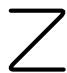
\includegraphics[keepaspectratio]{images/part002_abf04123.jpg}}

注. 注意，关系 \(\mathbf{f} \sim \mathbf{g}\) 决不蕴含差 \(\mathbf{f} - \mathbf{g}\) 沿 \(\mathfrak{F}\) 趋于 0；这个差甚至可以无界，正如例子 \(x^{2} + x \sim x^{2}\) （当 \(x\) 趋于 \(+\infty\) 时）所表明的。

命题 8. 设 K 是一个赋值域， \(f_{1}, f_{2}, g_{1}, g_{2}\) 是 \(\mathcal{H}(\mathfrak{F}, \mathrm{K})\) 中的四个函数；则关系 \(f_{1} \sim g_{1}\) 与 \(f_{2} \sim g_{2}\) 蕴含 \(f_{1}f_{2} \sim g_{1}g_{2}\) 。

事实上，我们有 \(f_{1}f_{2}-g_{1}g_{2}=f_{1}(f_{2}-g_{2})+(f_{1}-g_{1})g_{2}\) ；由于 \(f_{1}\preccurlyeq g_{1}\) 、 \(f_{1}-g_{1}\ll g_{1}\) 与 \(f_{2}-g_{2}\ll g_{2}\) ，我们有 \(f_{1}f_{2}-g_{1}g_{2}\ll g_{1}g_{2}\) (V, p.~215, prop. 5 and 6)。

相反，我们在 V, p.~214 中已给出一个例子，其中有 \(f_{1} = g_{1}\) 、 \(f_{2} \sim g_{2}\) ，然而关系 \(f_{1} + f_{2} \asymp g_{1} + g_{2}\) 并不成立（故更谈不上

\[
f _ {1} + f _ {2} \sim g _ {1} + g _ {2}).
\]

比较关系 \(f \ll g\) 、 \(f \sim g\) 称为强关系。 \(\mathcal{H}(\mathfrak{F}, V)\) 中的两个函数 f, g 称为可比较的（当想要避免任何可能的混淆时，称为强可比较的），如果它们满足下列三个关系之一： \(f \ll g\) 、 \(f \gg g\) ，或 “存在一个 \(\lambda \neq 0\) 使得 \(f \sim g\lambda\) ”。

注. 1) 两个函数可以是弱可比较的但不是强可比较的，例如函数 1 与 \(\sin x\) （当 \(x\) 趋于 \(+\infty\) 时）。

\begin{enumerate}
\def\labelenumi{\arabic{enumi})}
\setcounter{enumi}{1}
\tightlist
\item
  在比较关系 \(f_{1} \preccurlyeq f_{2}\) 与 \(f_{1} \ll f_{2}\) 的定义中，空间 \(V_{1}, V_{2}\) （ \(f_{1}\) 与 \(f_{2}\) 分别在其中取值）上的范数只是表面上介入；实际上介入的只是 \(V_{1}\) 与 \(V_{2}\) 上的拓扑，因为关系 \(f_{1} \preccurlyeq f_{2}\) 与 \(f_{1} \ll f_{2}\) 当把 \(V_{1}\) 或 \(V_{2}\) 上的范数换成一个等价范数时，就被等价的关系所代替 (Gen.~Top., IX, p.~170, def. 7)。
\end{enumerate}

\subsection{变量替换}

设 \(\varphi\) 是从集 \(E'\) 到 \(E\) 中的一个映射，使得 \(\overset{-1}{\varphi}(\mathfrak{F})\) 是 \(E'\) 上的一个滤子基。显然，若 \(\mathbf{f}_1, \mathbf{f}_2\) 分别是 \(\mathcal{H}(\mathfrak{F}, V_1)\) 与 \(\mathcal{H}(\mathfrak{F}, V_2)\) 中的函数，则 \(\mathbf{f}_1 \circ \varphi\) 、 \(\mathbf{f}_2 \circ \varphi\) 分别属于 \(\mathcal{H}(\overset{-1}{\varphi}(\mathfrak{F}), V_1)\) 与 \(\mathcal{H}(\overset{-1}{\varphi}(\mathfrak{F}), V_2)\) ，且关系 \(\mathbf{f}_1 \preccurlyeq \mathbf{f}_2\) （相应地， \(\mathbf{f}_1 \ll \mathbf{f}_2\) ）等价于 \(\mathbf{f}_1 \circ \varphi \preccurlyeq \mathbf{f}_2 \circ \varphi\) （相应地， \(\mathbf{f}_1 \circ \varphi \ll \mathbf{f}_2 \circ \varphi\) ）。

\subsection{严格正函数之间的比较关系}

设 \(g\) 是 \(\mathcal{H}(\mathfrak{F},\mathbf{R})\) 中的一个函数，它在 \(\mathfrak{F}\) 的某个集上严格正。涉及 \(g\) 的比较关系可以用另一种方式表述：关系 \(\mathbf{f} \preccurlyeq g\) 等价于说 \(\| \mathbf{f}\| /g\) （它定义在 \(\mathfrak{F}\) 的某个集上）在 \(\mathfrak{F}\) 的某个集上有界；关系 \(\mathbf{f} \ll g\) 等价于说 \(\| \mathbf{f}\| /g\) 沿 \(\mathfrak{F}\) 趋于 0。若 \(f\) 是 \(\mathcal{H}(\mathfrak{F},\mathbf{R})\) 中的一个函数，则关系 \(f\asymp g\) 表示 \(f / g\) 在 \(\mathfrak{F}\) 的某个集上对数有界，而关系 \(f\sim g\) 表示 \(f / g\) 沿 \(\mathfrak{F}\) 趋于 1。若 \(f\) 是 \(\mathcal{H}(\mathfrak{F},\mathbf{R})\) 中的一个函数且在 \(\mathfrak{F}\) 的某个集上为正，则说 \(f\) 与 \(g\) 可比较蕴含 \(f / g\) 趋于一个极限（有限的或等于 \(+\infty\) ，沿 \(\mathfrak{F}\) ）。

命题 9. 设 \(f\) 与 \(g\) 是 \(\mathcal{H}(\mathfrak{F},\mathbf{R})\) 中的两个函数，在 \(\mathfrak{F}\) 的某个集上严格正。为使 \(f\) 与 \(g\) 可比较，必要且充分的是：对每个数 \(t \geqslant 0\) （至多一个例外），函数 \(f - tg\) 具有常号 \(^3\) 于 \(\mathfrak{F}\) 的某个集上。

该条件是必要的。事实上，若 \(f \ll g\) ，则有 \(f - tg \sim -tg\) （ \(t = 0\) 除外），故 \(f - tg\) 在 \(\mathfrak{F}\) 的某个集上严格负（ \(t = 0\) 除外）；若 \(f \gg g\) ，则 \(f - tg\) 在 \(\mathfrak{F}\) 的某个集上严格正（对一切 \(t\) ）；最后，若 \(f \sim kg\) （ \(k\) 为常数 \(> 0\) ），则有 \(f - tg \sim (k - t)g\) （ \(t = k\) 除外），故除 \(t = k\) 可能例外外， \(f - tg\) 具有 \(k - t\) 的符号于 \(\mathfrak{F}\) 的某个集上。

该条件是充分的。事实上，设比值 \(f / g\) 有两个不同的聚点 \(\alpha < \beta\) （沿 \(\mathfrak{F}\) ）。于是对每个数 \(t\) （满足 \(\alpha < t < \beta\) ），在每个集 \(X \in \mathfrak{F}\) 中都存在两点 \(x_{1}, x_{2}\) ，使得 \(f(x_{1}) / g(x_{1}) < t\) 且 \(f(x_{2}) / g(x_{2}) > t\) ；从而 \(f(x) - tg(x)\) 在 \(X\) 上不具有常号；我们得到了一个与假设不相容的结论。由此推出， \(f / g\) 沿以 \(\mathfrak{F}\) 为基的滤子只能有一个聚值（有限的或无穷的），从而 (Gen.~Top., I, p.~85, corollary) 沿 \(\mathfrak{F}\) 以这个值为其极限。

命题 10. 设 \(f\) 与 \(g\) 是 \(\mathcal{H}(\mathfrak{F},\mathbf{R})\) 中的两个函数，在 \(\mathfrak{F}\) 的某个集上严格正；对每个实数 \(\alpha\) 且 \(\neq 0\) ，关系 \(f\asymp g\) （相应地， \(f\sim g\) ）等价于 \(f^{\alpha}\asymp g^{\alpha}\) （相应地， \(f^{\alpha}\sim g^{\alpha}\) ）；若 \(\alpha >0\) ，关系 \(f\preccurlyeq g\) （相应地， \(f\ll g\) ）等价于 \(f^{\alpha}\preccurlyeq g^{\alpha}\) （相应地， \(f^{\alpha}\ll g^{\alpha}\) ）；若 \(\alpha < 0\) ，它等价于 \(f^{\alpha}\succcurlyeq g^{\alpha}\) （相应地， \(f^{\alpha}\gg g^{\alpha}\) ）。

证明都是直接的。

我们注意到，在 \(\mathcal{H}(\mathfrak{F},\mathbf{R})\) 中，在 F 的某个集上严格正的函数所成的集 \(\varGamma\) 使得 \(\varGamma/\mathrm{R}_{\infty}\) 是一个乘法群 \(\varGamma_{\infty}\) （在 \(\mathcal{H}_{\infty}(\mathfrak{F},\mathbf{R})\) 中）； \(\varGamma/\mathrm{R}_{0}\) 恒同于 \(\varGamma_{\infty}\) 关于（模 \(R_{\infty}\) ） \(\varGamma\) 中对数有界函数的类所成的子群的商群；在 \(\varGamma/R_{0}\) 上，由关系 \(f \preccurlyeq g\) 通过过渡到商而导出的序关系与 \(\varGamma/R_{0}\) 的群结构相容，从而使之成为一个有序群。

命题 11. 设 g 是 \(\mathcal{H}(\mathfrak{F},\mathbf{R})\) 中的一个函数，使得 \(\lim_{\mathfrak{F}}g = +\infty\) ；则关系 \(f \ll g\) 蕴含 \(e^{f} \ll e^{g}\) ；关系 \(f \sim g\) 蕴含 \(\log f \sim \log g\) 。

事实上，若 \(f \ll g\) ，则 \(f - g = g\left(\frac{f}{g} - 1\right)\) 趋于 \(-\infty\) （沿 \(\mathfrak{F}\) ）。类似地，若 \(f \sim g\) ，则有 \(\log f = \log g + \log \frac{f}{g}\) ，故 \(\log f - \log g\) 趋于 0，对 \(\frac{\log f}{\log g} - 1 = \frac{\log f - \log g}{\log g}\) 亦然。

\pandocbounded{
\includegraphics[keepaspectratio]{images/part002_2162bedd.jpg}}

另一方面，注意关系 \(f \sim g\) 并不蕴含 \(e^{f} \sim e^{g}\) ，甚至不蕴含 \(e^{f} \asymp e^{g}\) ，正如例子 \(f(x) = x^{2}\) 、 \(g(x) = x^{2} + x\) （当 x 趋于 \(+\infty\) 时）所表明的；类似地，关系 \(f \ll g\) 并不蕴含 \(\log f \ll \log g\) ，正如例子 \(f(x) = x\) 、 \(g(x) = x^{2}\) （当 x 趋于 \(+\infty\) 时）所表明的。

定义 5. 设 g 是 \(\mathcal{H}(\mathfrak{F},\mathbf{R})\) 中的一个函数，在 F 的某个集上严格正，且使得 \(\lim_{\mathfrak{F}}g=0\) 或 \(\lim_{\mathfrak{F}}g=+\infty\) 。我们说函数 \(f\in\mathcal{H}(\mathfrak{F},\mathbf{R})\) 相对于 g 是 \(\rho\) 阶的（有限或无穷），如果 \(\lim_{\mathfrak{F}}\log(|f|)/\log g=\rho\) 。

注意，若 f 相对于 g 是 \(\rho\) 阶的，则 f 相对于 1/g 是 \(-\rho\) 阶的；因此只需处理 \(g(x)\) 沿 F 趋于 \(+\infty\) 的情形。

\pandocbounded{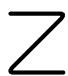
\includegraphics[keepaspectratio]{images/part002_5139c9a2.jpg}}

命题 12. 设 \(g\) 是 \(\mathcal{H}(\mathfrak{F},\mathbf{R})\) 中的一个函数，使得 \(\lim_{\mathfrak{F}}g = +\infty\) ；设 \(f\) 是 \(\mathcal{H}(\mathfrak{F},\mathbf{R})\) 中的一个函数。

\begin{enumerate}
\def\labelenumi{\alph{enumi})}
\item
  为使 \(f\) 是 \(+\infty\) 阶的（相对于 \(g\) ），必要且充分的是 \(f \gg g^{\alpha}\) （对每个 \(\alpha \geqslant 0\) ）。
\item
  为使 \(f\) 是 \(-\infty\) 阶的（相对于 \(g\) ），必要且充分的是 \(f \ll g^{-\alpha}\) （对每个 \(\alpha > 0\) ）。
\item
  为使 \(f\) 是等于 \(\rho\) 的有限阶（相对于 \(g\) ），必要且充分的是：对每个 \(\varepsilon > 0\) ，有 \(g^{\rho - \varepsilon} \ll f \ll g^{\rho + \varepsilon}\) 。
\end{enumerate}

例如我们证明 c)。若 \(f\) 相对于 \(g\) 的阶是 \(\rho\) ，则对每个 \(\varepsilon > 0\) ，存在一个集 \(\mathbf{M} \in \mathfrak{F}\) ，使得对每个 \(x \in \mathbf{M}\) ，我们有

\[
\left(\rho - \frac {\varepsilon}{2}\right) \log g (x) \leqslant \log | f (x) | \leqslant \left(\rho + \frac {\varepsilon}{2}\right) \log g (x),
\]

或者 \((g(x))^{\rho-\frac{\varepsilon}{2}} \leqslant |f(x)| \leqslant (g(x))^{\rho+\frac{\varepsilon}{2}}\) ；由于 \(\lim_{\mathfrak{F}} g = +\infty\) ，于是有 \(g^{\rho-\varepsilon} \ll f \ll g^{\rho+\varepsilon}\) （对每个 \(\varepsilon > 0\) ）；其逆是直接的。a) 与 b) 的证明类似。

注意，若 \(f\) 是有限阶 \(\rho\) （相对于 \(g\) ），则 \(fg^{-\rho}\) 相对于 \(g\) 是 0 阶，反之亦然；若 \(f_1\) （相应地， \(f_2\) ）是 \(\rho_1\) 阶（相应地， \(\rho_2\) 阶）的（相对于 \(g\) ），且 \(\rho_1 + \rho_2\) 有定义，则 \(f_1f_2\) 是 \(\rho_1 + \rho_2\) 阶的（相对于 \(g\) ）。

注. 1) 注意，尽管 f 相对于 g 可以是有限阶 \(\rho\) ，但比值 \(f/g^{\rho}\) 未必趋于一个极限；例如，每个对数有界函数相对于 g 都是 0 阶的，但沿 F 未必有极限。

\begin{enumerate}
\def\labelenumi{\arabic{enumi})}
\setcounter{enumi}{1}
\tightlist
\item
  一个定义在 \(\mathfrak{F}\) 的某个集上的函数未必相对于 \(g\) 有确定的阶（有限的或否），因为相对于 \(g\) 有确定阶的函数与 \(g\) 的一切幂可比较（至多一个例外）。而 \(f\) 未必具有这个性质，例子 \(g(x) = x\) 、 \(f(x) = 1 + x^2 \sin^2 x\) （当 \(x\) 趋于 \(+\infty\) 时）便表明了这一点。在这个例子中， \(f\) 与 \(g^\alpha\) 可比较（对 \(\alpha < 0\) 与 \(\alpha > 2\) ）；若取 \(f(x) = e^x \sin^2 x + e^{-x} \cos^2 x\) ，则 \(f\) 不与 \(g\) 的任何幂（正的或负的）可比较。
\end{enumerate}

\subsection{记号}

给定一个实函数 \(f \in \mathcal{H}(\mathfrak{F}, \mathbf{R})\) ，在一个公式中用 \(O(f)\) 表示一个受 \(f\) 控制的函数、用 \(o(f)\) 表示一个相对于 \(f\) 可忽略的函数，这往往是方便的。当在一个证明中出现多个受同一个函数 \(f\) 控制的（相应地，相对于 \(f\) 可忽略的）函数时，我们把它们记作 \(O_1(f)\) 、 \(O_2(f)\) 等（相应地， \(o_1(f)\) 、 \(o_2(f)\) 等）。

许多作者不加区分地把一个证明中所有受 f 控制的（相应地，相对于 f 可忽略的）函数都记作 \(O(f)\) （相应地， \(o(f)\) ），这是一种可能引起混淆的语言滥用。

用这个记号，我们可以把命题 1、2、3 (V, p.~213) 表述如下：若 \(g = O_1(f)\) 且 \(h = O(g)\) ，则 \(h = O_2(f)\) ；我们可以写

\[
\sum_ {i = 1} ^ {n} \lambda_ {i} O _ {i} (f) = O _ {n + 1} (f) \quad (\lambda_ {i} \text {   scalars })\tag{1}
\]

\[
O (f) O (g) = O (f g).\tag{2}
\]

类似地，命题 4 (V, p.~215) 表明，若 \(g = O_1(f)\) 且 \(h = o(g)\) （相应地， \(g = o_1(f)\) 且 \(h = O(g)\) ），则 \(h = o_2(f)\) ，而命题 5 与 6 (V, p.~5) 可以表述成形式

\[
\sum_ {i = 1} ^ {n} \lambda_ {i} o _ {i} (f) = o _ {n + 1} (f) \quad (\lambda_ {i} \text {   scalars })\tag{3}
\]

\[
o (f) O (g) = o (f g).\tag{4}
\]

关系 \(f \sim g\) 等价于 \(f = g + o(g)\) 。记号 \(O(1)\) （相应地， \(o(1)\) ）表示在 \(\mathfrak{F}\) 的某个集上有界的一个函数（相应地，沿 \(\mathfrak{F}\) 趋于 0 的一个函数）。

\section{渐近展开}

\subsection{比较尺度}

设 E 是一个被具有基 F 的滤子所滤过的集，K 是一个非离散赋值域（最常见的是 K = R 或 K = C）。在 \(\mathcal{H}(\mathfrak{F}, \mathrm{K})\) 中模 \(R_{\infty}\) 不等价于 0 的函数（即在 F 的每个集中至少有一点使函数不为零的那些函数）所成的集中，关系 “ \(f \ll g\) 或 f = g” 是一个序关系。

定义 1. 我们说 \(\mathcal{H}(\mathfrak{F},\mathrm{K})\) 的一个由模 \(R_{\infty}\) 不等价于 0 的函数组成的子集 E 是一个比较尺度，如果 E 被关系 “ \(f \ll g\) 或 f = g” 全序化。

换句话说，若 \(f\) 与 \(g\) 是 \(\mathcal{E}\) 中的函数，则关系 \(f \ll g\) 、 \(g \ll f\) 、 \(f = g\) 中总有一个（且只有一个）成立。由此推出，在 \(\mathcal{E}\) 上关系 \(f \asymp g\) （更不用说 \(|f| \sim a |g|\) ，其中 \(a\) 是一个数 \(> 0\) ）蕴含 \(f = g\) 。

一个比较尺度的每个子集显然也是一个比较尺度。

例. 1) 对实的且趋于 \(+\infty\) 的 x，函数 \(x^{\alpha}\) （ \(\alpha\) 为任意实数）所成的集是一个比较尺度。当 F 是以 a 为左端点的开区间所成的集时，函数 \((x - a)^{\alpha}\) 亦然。

\begin{enumerate}
\def\labelenumi{\arabic{enumi})}
\setcounter{enumi}{1}
\item
  当复数 \(z\) 趋于 \(\infty\) 时，函数 \(z^n\) （ \(n\) 为有理整数）所成的集是一个比较尺度；函数 \((z - a)^n\) 亦然（当 \(\mathfrak{F}\) 是该点的邻域滤子在点 \(a \in \mathbf{C}\) 的余集上的迹时）。
\item
  设 F 是赋范空间；当 F 是该点的邻域滤子在 a 的余集上的迹时，函数族 \(\|\mathbf{x}-\mathbf{a}\|^{\alpha}\) （ \(\alpha\) 为任意实数）是一个比较尺度。注意，若 p 与 q 是 F 上两个不同的范数，则两个比较尺度 \(\left(p(\mathbf{x}-\mathbf{a})\right)^{\alpha}\) 与 \(\left(q(\mathbf{x}-\mathbf{a})\right)^{\alpha}\) 的并一般不是一个比较尺度。
\item
  当实数 \(x\) 趋于 \(+\infty\) 时，函数族 \(\mathcal{E}\) 由形如 \(\exp(p(x))\) 的函数（其中 \(p\) 取遍无常数项的（实系数）多项式所成的集）组成，它是一个比较尺度：只需注意， \(\mathcal{E}\) 中两个函数的商仍在 \(\mathcal{E}\) 中，且函数 \(\exp(p(x))\) 必趋于 0 或 \(+\infty\) （如果 \(p \neq 0\) ）；事实上， \(p(x) \sim \alpha x^n\) （其中 \(n > 0\) 且 \(\alpha \neq 0\) ）；若 \(\alpha > 0\) ，则有 \(p(x) > \frac{1}{2}\alpha x^n\) （对充分大的 \(x\) ）；若 \(\alpha < 0\) ，则有 \(p(x) < \frac{1}{2}\alpha x^n\) （对充分大的 \(x\) ）；在第一种情形 \(\exp(p(x))\) 趋于 \(+\infty\) ，在第二种情形趋于 0。
\item
  对实的且趋于 \(+\infty\) 的 x，形如 \(x^{\alpha}(\log x)^{\beta}\) （对 x \textgreater{} 1 有定义）的函数所成的集 E（其中 \(\alpha\) 与 \(\beta\) 为任意实数）是一个比较尺度。事实上，这里同样，E 中两个函数的商是 E 中的一个函数；只需证明：若 \(\alpha\) 与 \(\beta\) 不全为零，则 \(x^{\alpha}(\log x)^{\beta}\) 趋于 0 或 \(+\infty\) ；这在 \(\alpha = 0, \beta \neq 0\) 时是明显的；若 \(\alpha > 0\) ，有 \((\log x)^{-\beta} \ll x^{\alpha}\) ，而若 \(\alpha < 0\) ，有 \((\log x)^{\beta} \ll x^{-\alpha}\) （对任何 \(\beta\) ），由此得命题。
\end{enumerate}

注意，最后这个比较尺度是一个全序集（对关系 “ \(f \ll g\) 或 \(f = g\) ”），其序结构同构于 \(R^{2}\) 上的字典序 (Set Theory, III, p.~157)；回忆在这个结构中关系 \((\alpha, \beta) < (\gamma, \delta)\) 表示 “ \(\alpha < \gamma\) ，或 \(\alpha = \gamma\) 且 \(\beta < \delta\) ”。

类似地，由函数 \(\exp(p(x))\) （其中 p 取遍无常数项多项式所成的集 \(P_{0}\) ）组成的尺度具有同构于 \(P_{0}\) 的序结构的序结构，在其中关系 p \textless{} q 表示多项式 q - p 的主导项具有 \textgreater{} 0 的系数 (cf.~Alg., VI. 19, 例 2)。

设 \(\varphi\) 是从集 \(F\) 到 \(E\) 中的一个映射，使得 \(\overset{-1}{\varphi}(\mathfrak{F})\) 是 \(F\) 上的一个滤子基。若 \(\mathcal{E}\) 是 \(E\) 上的一个比较尺度（对滤子基 \(\mathfrak{F}\) ），则函数 \(f \circ \varphi\) （当 \(f\) 取遍 \(\mathcal{E}\) ）在 \(F\) 上组成一个比较尺度（对滤子基 \(\overset{-1}{\varphi}(\mathfrak{F})\) ）。

\subsection{主部与渐近展开}

设 E 是一个由取值于非离散赋值域 K 中的函数组成的比较尺度。设 V 是 K 上的一个赋范空间，f 是 \(\mathcal{H}(\mathfrak{F}, V)\) 中的一个函数；如果存在一个函数 \(g \in E\) 和 V 中的一个元素 \(a \neq 0\) 使得 \(f \sim ag\) ，就说 ag 是 f 相对于尺度 E 的一个主部。由 V, p.~10 的定义 1，f 相对于 E 只能有一个主部，因为若 \(g_{1}\) 、 \(g_{2}\) 是 E 中的两个函数且 \(a_{1}\) 、 \(a_{2}\) 是 V 中两个 \(\neq 0\) 的元素，则关系 \(a_{1}g_{1} \sim a_{2}g_{2}\) 蕴含 \(|g_{1}| \asymp |g_{2}|\) ，从而 \(g_{1} = g_{2}\) ，于是 \((\mathbf{a}_{2} - \mathbf{a}_{1})g_{1} \ll g_{1}\) ，而由于 \(g_{1}\) 在 E 的任何集上都不恒为零，这蕴含 \(a_{2} = a_{1}\) 。

若 f 相对于一个比较尺度 E 有主部，则它相对于每个比较尺度 \(E' \supset E\) 有同一主部。

例. 1) 对实的（相应地，复的）且趋于 \(+\infty\) （相应地， \(\infty\) ）的 x，每个多项式 \(a_{0}x^{n} + a_{1}x^{n-1} + \ldots + a_{n}\) （系数在 V 中，且 \(a_{0} \neq 0\) ）以 \(a_{0}x^{n}\) 为主部（相对于尺度 \(x^{n}\) ，或任何包含 \(x^{n}\) 的尺度）。由此推出，每个有理分式 \(\frac{a_{0}x^{n} + \cdots + a_{m}}{b_{0}x^{n} + \cdots + b_{n}}\) （实或复系数，且 \(a_{0}b_{0} \neq 0\) ）相对于同一尺度以 \(\frac{a_{0}}{b_{0}}x^{m-n}\) 为主部。

\begin{enumerate}
\def\labelenumi{\arabic{enumi})}
\setcounter{enumi}{1}
\tightlist
\item
  一个函数可以与一个尺度的所有函数可比较，却相对于该尺度没有主部。例如，当实数 \(x\) 趋于 \(+\infty\) 时， \(\sqrt{x}\) 相对于尺度 \(x^n\) （其中 \(n\) 为有理整数）没有主部； \(\log x\) 相对于 \(x^\alpha\) （ \(\alpha\) 任意实）的尺度没有主部； \(\exp(\sqrt{\log x})\) 与 \(x^x = e^{x\log x}\) 相对于 \(x^\alpha (\log x)^\beta\) 的尺度没有主部，也不相对于 \(\exp(p(x))\) （ \(p\) 为无常数项多项式）的尺度有主部。
\end{enumerate}

主部的概念容许广泛的推广。设函数 \(\mathbf{f} \in \mathcal{H}(\mathfrak{F}, V)\) 有主部 \(\mathbf{a}_1g_1\) （相对于尺度 \(\mathcal{E}\) ）；关系 \(\mathbf{f} \sim \mathbf{a}_1g_1\) 等价于 \(\mathbf{f} - \mathbf{a}_1g_1 \ll g_1\) (V, p.~216, def. 4)；为更细致地研究函数 \(\mathbf{f}\) ，我们因而被引导去考虑函数 \(\mathbf{f} - \mathbf{a}_1g_1\) 。若这个函数有主部 \(\mathbf{a}_2g_2\) （相对于 \(\mathcal{E}\) ），则必有 \(g_2 \ll g_1\) 且 \(\mathbf{f} - \mathbf{a}_1g_1 - \mathbf{a}_2g_2 \ll g_2\) 。

更一般地，设尺度 E 以参数形式写成 \((g_{\alpha})\) ，其中 \(\alpha\) 取遍一个指标集 A，它被赋予一个同构于 E 的序结构的反序的全序结构：于是关系 \(\alpha < \beta\) 等价于 \(g_{\beta} \ll g_{\alpha}\) 。在这些条件下：

定义 2. 我们说函数 \(\mathbf{f} \in \mathcal{H}(\mathfrak{F}, V)\) 容许一个精确到 \(g_{\alpha}\) 的渐近展开（相对于尺度 \(\mathcal{E}\) ），如果存在 V 的元素的一个族 \((\mathbf{a}_{\lambda})_{\lambda \leqslant \alpha}\) （除有限多个外全为 0），使得 \(\mathbf{f} - \sum_{\lambda \leqslant \alpha} \mathbf{a}_{\lambda} g_{\lambda} \ll g_{\alpha}\) 。我们说 \(\sum_{\lambda \leqslant \alpha} \mathbf{a}_{\lambda} g_{\lambda}\) 是 \(\mathbf{f}\) 的一个精确到 \(g_{\alpha}\) 的渐近展开， \(\mathbf{a}_{\lambda} g_{\lambda} (\lambda \leqslant \alpha)\) 是它的项， \(\mathbf{a}_{\lambda}\) 是它的系数，而函数 \(\mathbf{r}_{\alpha} = \mathbf{f} - \sum_{\lambda \leqslant \alpha} \mathbf{a}_{\lambda} g_{\lambda}\) 是这个展开的余项。

为表示 \(\sum_{\lambda \leqslant \alpha} \mathbf{a}_{\lambda} g_{\lambda}\) 是 \(\mathbf{f}\) 的一个精确到 \(g_{\alpha}\) 的渐近展开这一事实，最常见的是只写

\[
\mathbf {f} = \sum_ {\lambda \leqslant \alpha} \mathbf {a} _ {\lambda} g _ {\lambda} + o (g _ {\alpha}) \quad (\text { or } \mathbf {f} = \sum_ {\lambda \leqslant \alpha} \mathbf {a} _ {\lambda} g _ {\lambda} + o _ {k} (g _ {\alpha})
\]

如果证明中有多个函数），遵循 V, p.~219 与 220 的记号。

对于相对于同一尺度 E 的两个渐近展开（两个函数的，相同与否），我们说精确度指标较大的那个更精确。

若 \(\sum_{\lambda \leqslant \alpha} \mathbf{a}_{\lambda} g_{\lambda}\) 是 \(\mathbf{f}\) 的一个精确到 \(g_{\alpha}\) 的渐近展开，则对每个 \(\beta < \alpha\) ， \(\sum_{\lambda \leqslant \beta} \mathbf{a}_{\lambda} g_{\lambda}\) 是 \(\mathbf{f}\) 的一个精确到 \(g_{\beta}\) 的渐近展开 (V, p.~215, prop. 5)：说它是通过把给定展开 \(\sum_{\lambda \leqslant \alpha} \mathbf{a}_{\lambda} g_{\lambda}\) （ \(\mathbf{f}\) 的）的精确度降到 \(g_{\beta}\) 而得到的。

若 \(\sum_{\lambda \leqslant \alpha} \mathbf{a}_{\lambda} g_{\lambda}\) 与 \(\sum_{\lambda \leqslant \alpha} \mathbf{b}_{\lambda} g_{\lambda}\) 是同一精确度 \(g_{\alpha}\) 的渐近展开（两个函数 \(\mathbf{f}_1, \mathbf{f}_2\) 的），则 \(\sum_{\lambda \leqslant \alpha} (\mathbf{a}_{\lambda} + \mathbf{b}_{\lambda}) g_{\lambda}\) 是 \(\mathbf{f}_1 + \mathbf{f}_2\) 的一个精确到

精确度 \(g_{\alpha}\) (V, p.~215, prop. 5)；且对每个标量 \(c\) ， \(\sum_{\lambda \leqslant \alpha} \mathbf{a}_{\lambda}cg_{\lambda}\) 是 \(\mathbf{f}_1c\) 的一个精确到 \(g_{\alpha}\) 的渐近展开。由此推出，若一个函数容许一个精确到 \(g_{\alpha}\) 的渐近展开，则这个展开是唯一的：只需看到函数 0 不容许一个精确度 \(g_{\alpha}\) 的、具有 \(\neq 0\) 系数的渐近展开。因为，若 \(0 = \sum_{\lambda \leqslant \alpha} \mathbf{a}_{\lambda}g_{\lambda} + \mathbf{r}_{\alpha}\) ，且 \(\gamma\) 是指标 \(\lambda \leqslant \alpha\) （使 \(\mathbf{a}_{\lambda} \neq 0\) 者）中最小者，则将有 \(\mathbf{a}_{\gamma}g_{\gamma} = -\sum_{\gamma < \lambda \leqslant \alpha} \mathbf{a}_{\lambda}g_{\lambda} - \mathbf{r}_{\alpha} \ll g_{\gamma}\) ，这是荒谬的。

说一个函数 \(\mathbf{f}\) 容许一个精确到 \(g_{\alpha}\) 的渐近展开且其系数全为零，等价于说 \(\mathbf{f} \ll g_{\alpha}\) 。若 \(\mathbf{f}\) 容许一个渐近展开 \(\sum_{\lambda \leqslant \alpha} \mathbf{a}_{\lambda} g_{\lambda}\) （精确到 \(g_{\alpha}\) ），其系数不全为零，且 \(\gamma\) 是指标 \(\lambda\) （使 \(\mathbf{a}_{\lambda} \neq 0\) 者）中最小者，则 \(\mathbf{a}_{\gamma} g_{\gamma}\) 是 \(\mathbf{f}\) 相对于尺度 \(\mathcal{E}\) 的主部，因为有 \(\mathbf{f} - \mathbf{a}_{\gamma} g_{\gamma} = \sum_{\gamma < \lambda \leqslant \alpha} \mathbf{a}_{\lambda} g_{\lambda} + \mathbf{r}_{\alpha} \ll g_{\gamma}\) ；类似地，若 \(\mu \leqslant \alpha\) 是使 \(\mathbf{a}_{\mu} \neq 0\) 的一个指标，则 \(\mathbf{a}_{\mu} g_{\mu}\) 是 \(\mathbf{f} - \sum_{\lambda < \mu} \mathbf{a}_{\lambda} g_{\lambda}\) 的主部。

在应用中最重要的渐近展开是相对于 \(x^{-n}\) （相应地， \(z^{-n}\) ）的尺度的那些，其中 n 是正或负整数，当 x 趋于 \(+\infty\) 或 \(-\infty\) （相应地，当复数 z 趋于 \(\infty\) ）时；或相对于 \((x - c)^{n}\) （相应地， \((z - c)^{n}\) ）的尺度的那些，当实数 x 从右边或左边趋于 c（相应地，当复数 z 趋于 c）时。我们在 I, p.~21 中已看到，在一点 \(c \in R\) 处 k 次可导的每个实变量 x 的向量函数在该点容许一个 k 阶泰勒展开，即一个精确到 \((x - c)^{k}\) 的、相对于 \((x - c)^{n}\) 的尺度的渐近展开。

\subsection{渐近展开的和与积}

若 \(f_{1}\) 、 \(f_{2}\) 相对于一个比较尺度 E 分别容许精确到 \(g_{\alpha}\) 与 \(g_{\beta}\) 的渐近展开，则通过把两个展开限制到这个精确度，可导出精确到 \(g_{\min(\alpha,\beta)}\) 的展开；我们已在 V, p.~222 中看到如何得到 \(f_{1} + f_{2}\) 的一个精确到 \(g_{\min(\alpha,\beta)}\) 的渐近展开。

设 \(V_{1}, V_{2}\) 与 V 是域 K 上的三个赋范空间，并设 \((\mathbf{x}, \mathbf{y}) \mapsto [\mathbf{x}, \mathbf{y}]\) 是从 \(V_{1} \times V_{2}\) 到 V 中的一个连续双线性映射；对本节的其余部分，我们进一步假设尺度 E 使得 E 中任意两个函数的乘积仍在 E 中（这对所有作为例子给出的比较尺度（在 V, p.~220 中）都成立）。

现在设 \(f_{1}\) 、 \(f_{2}\) 分别是 \(\mathcal{H}(\mathfrak{F}, V_{1})\) 与 \(\mathcal{H}(\mathfrak{F}, V_{2})\) 中的两个函数，分别具有渐近展开 \(f_{1} = \sum_{\lambda \leqslant \alpha} a_{\lambda} g_{\lambda} + r_{\alpha}\) 与 \(f_{2} = \sum_{\mu \leqslant \beta} b_{\mu} g_{\mu} + r_{\beta}\) （精确度分别为 \(g_{\alpha}\) 与 \(g_{\beta}\) ，相对于尺度 E）。进一步假设 \(a_{\lambda}\) 与 \(b_{\mu}\) 都不全为零，并设 \(a_{\gamma} g_{\gamma}\) 与 \(b_{\delta} g_{\delta}\) 是 \(f_{1}\) 与 \(f_{2}\) 的主部。根据假设，可以写 \(g_{\gamma} g_{\beta} = g_{\rho}\) 与 \(g_{\delta} g_{\alpha} = g_{\sigma}\) ；让我们证明：和 \(\sum[a_{\lambda}.b_{\mu}]g_{\lambda}g_{\mu}\) （对所有对 \((\lambda,\mu)\) （满足 \(g_{\min(\rho,\sigma)}\ll g_{\lambda}g_{\mu}\) ）取的）是 \([f_{1}.f_{2}]\) 的一个精确到 \(g_{\min(\rho,\sigma)}\) 的渐近展开。现在 \([f_{1}.f_{2}]\) 与这个和的差是有限多个项之和，其中每一项或者形如 \([a_{\lambda}.b_{\mu}]g_{\lambda}g_{\mu}\) （满足 \(g_{\lambda}g_{\mu}\ll g_{\min(\rho,\sigma)}\) ），或者形如 \([a_{\lambda}.r_{\beta}]g_{\lambda}\) （其中 \(\lambda\geqslant\gamma\) ），或者形如 \([r_{\alpha}.b_{\mu}]g_{\mu}\) （其中 \(\mu\geqslant\delta\) ）；但由于 {[}x.y{]} 连续，由 (V, p.~213, prop. 3 and V, p.~215, prop. 6) 有 \([a_{\lambda}.r_{\beta}]g_{\lambda}\preccurlyeq r_{\beta}g_{\lambda}\ll g_{\beta}g_{\gamma}=g_{\rho}\) （对 \(\lambda\geqslant\gamma\) ），类似地 \([r_{\alpha}.b_{\mu}]g_{\mu}\preccurlyeq r_{\alpha}g_{\mu}\ll g_{\alpha}g_{\delta}=g_{\sigma}\) （对 \(\mu\geqslant\delta\) ），由此得命题 (V, p.~215, prop. 5)。

若所有 \(a_{\lambda}\) 为零，则 \([f_{1}.f_{2}] \ll g_{\alpha}g_{\delta}\) ；换句话说，有 \([f_{1}.f_{2}]\) 的一个零项的、精确到 \(g_{\alpha}g_{\delta}\) 的渐近展开；类似地，若所有 \(a_{\lambda}\) 与 \(b_{\mu}\) 为零，则有 \([f_{1}.f_{2}]\) 的一个零项的、精确到 \(g_{\alpha}g_{\beta}\) 的渐近展开。

我们将把上述结果主要应用于 V 是 K 上的赋范代数且双线性函数 \([x.y]\) 是这个代数中的乘积 xy 的情形；最重要的情形是 V 等于 R 或 C 的情形。

特别地，若 \(f_{i}\) （ \(1 \leqslant i \leqslant n\) ）是 \(\mathcal{H}(\mathfrak{F}, \mathrm{K})\) 中的 n 个函数，其中每个都相对于 E 容许一个渐近展开，则对每个多项式 \(\sum_{(v_{i})} a_{v_{1}v_{2}\ldots v_{n}} f_{1}^{v_{1}} \ldots f_{n}^{v_{n}}\) （ \(f_{i}\) 的，系数在赋范空间 V 中）都可以得到一个相对于 E 的渐近展开；此外，前面的规则使我们能确定所得到的展开的精确度，只要我们知道函数 \(f_{i}\) 的展开的精确度。

\subsection{渐近展开的复合}

设 f 是 \(\mathcal{H}(\mathfrak{F},\mathbf{R})\) （相应地， \(\mathcal{H}(\mathfrak{F},\mathbf{C})\) ）中的一个函数，它容许一个相对于尺度 E 的、精确到 \(g_{\alpha}\) 的渐近展开，并且沿以 F 为基的滤子有极限 0。另一方面，设 h 是一个取值于 R（相应地， C）上的赋范空间 V 中的函数，定义在 R（相应地， C）中点 0 的一个邻域上，且在这个邻域上 n 次可导；则

\[
\mathbf {h} (t) = \mathbf {c} _ {0} + \mathbf {c} _ {1} t + \dots + \mathbf {c} _ {n} t ^ {n} + o (t ^ {n})
\]

在这个邻域上成立 (I, p.~21)，由此，在 \(\mathfrak{F}\) 的一个适当的集上

\[
\mathbf {h} \circ f = \mathbf {c} _ {0} + \mathbf {c} _ {1} f + \dots + \mathbf {c} _ {n} f ^ {n} + o (f ^ {n}).
\]

我们已在第 3 节中看到，如何为 \(c_{0} + c_{1}f + \cdots + c_{n}f^{n}\) 构造一个精确到 \(g_{\rho}\) 的渐近展开，其精确度由 f 的展开的精确度确定；此外，设 f 的渐近展开的系数不全为零，且 \(a_{\gamma}g_{\gamma}\) 是 f 的主部，并设 \(g_{\sigma} = g_{\gamma}^{n}\) ；若 \(\sigma < \rho\) ，则将得到 \(h \circ f\) 的一个精确到 \(g_{\sigma}\) 的展开（通过把 \(\sum_{k=0}^{n} c_{k}f^{k}\) 的展开限制到这个精确度）；反之，若 \(\rho \leqslant \sigma\) ，则 \(\sum_{k=0}^{n} c_{k}f^{k}\) 的展开也是 \(h \circ f\) 的一个精确到 \(g_{\rho}\) 的展开。

若 \(f\) 的渐近展开的所有项为零，且 \(g_{\alpha} \ll 1\) ，则 \(f \ll g_{\alpha}\) ，从而 \(f^k \ll g_{\alpha}^k \ll g_{\alpha}\) （对每个整数 \(k > 0\) ）；若 \(\mathbf{c}_m\) 是指标 \(> 0\) 的第一个不为零的系数（假设 \(\mathbf{c}_k\) 对指标 \(k > 0\) 不全为 0），则 \(\mathbf{c}_0\) 是 \(\mathbf{h} \circ f\) 的一个精确到 \(g_{\alpha}^{m}\) 的渐近展开。

在本节的其余部分，我们将限于 \(\mathcal{E}\) 中的函数取实值且在 \(\mathfrak{F}\) 的某个集上严格正的情形，并且只考虑 \(\mathcal{H}(\mathfrak{F},\mathbf{R})\) 中函数的渐近展开。首先假设对每个函数 \(g\in \mathcal{E}\) 和每个实数 \(\nu\) ， \(g^{\nu}\) 仍属于 \(\mathcal{E}\) ：这个条件例如被 \(x^{\alpha}\) 的尺度或 \(x^{\alpha}|\log x|^{\beta}\) 的尺度（ \(\alpha\) 与 \(\beta\) 为任意实数）在 \(+\infty\) 的一个邻域上或在 \(\mathbf{R}\) 中 0 的一个邻域上满足。这个性质蕴含 \(\mathcal{E}\) 中两个函数的商仍属于 \(\mathcal{E}\) 。这样，从相对于 \(\mathcal{E}\) 的、函数 \(f\in \mathcal{H}(\mathfrak{F},\mathbf{R})\) 的一个精确到 \(g_{\alpha}\) 的渐近展开，可导出 \(|f|^{\nu}\) 的一个展开（对每个实数 \(\nu\) ）。让我们限于 \(f\) 的展开的系数不全为零的情形，并设 \(a_{\gamma}g_{\gamma}\) 是 \(f\) 的主部；可以写 \(|f|^{\nu} = |a_{\gamma}|^{\nu}g_{\gamma}^{\nu}(1 + h)^{\nu}\) ，其中

\[
h = \sum_ {\gamma <   \lambda \leqslant \alpha} \frac {a _ {\lambda}}{a _ {\gamma}} \frac {g _ {\lambda}}{g _ {\gamma}} + o \left(\frac {g _ {\alpha}}{g _ {\gamma}}\right).
\]

在我们的假设下， \(\sum_{\gamma < \lambda \leqslant \alpha} \frac{a_{\lambda}}{a_{\gamma}} \frac{g_{\lambda}}{g_{\gamma}}\) 是 \(h\) 的一个渐近展开（精确到 \(g_{\alpha} / g_{\gamma}\) ）；由于 \(h\) 沿 \(\mathfrak{F}\) 趋于 0，上面描述的方法给出 \((1 + h)^{\nu}\) 的一个渐近展开，然后得到 \(|f|^{\nu}\) 的一个展开（通过乘以 \(\left|a_{\gamma}\right|^{\nu} g_{\gamma}^{\nu}\) ）。

对 \(f\) 用同样的假设，可以写

\[
\log | f | = \log \left| a _ {\gamma} g _ {\gamma} \right| + \log (1 + h)
\]

并且 \(\log(1+h)\) 可以展开，如上所述，因为函数 \(\log(1+t)\) 在 0 的一个邻域上是无穷次可导的；此外，若 \(\log g_{\gamma}\) 相对于 E 容许一个渐近展开，或相对于某个尺度 \(E_{1} \supset E\) 容许一个渐近展开，则在把这两个渐近展开相加后得到 \(\log|f|\) 的一个渐近展开。

例. 我们有 \((1+x)^{1/x}=\exp\left(\frac{1}{x}\log(1+x)\right)\) ；当 x 趋于 \(+\infty\) 时，我们有 \(\log(1+x)=\log x+\log\left(1+\frac{1}{x}\right)\) ，由此得 \(\frac{1}{x}\log(1+x)\) 的相对于 \(x^{\alpha}(\log x)^{\beta}\) 的尺度的渐近展开：

\[
\frac {1}{x} \log (1 + x) = \frac {\log x}{x} + \frac {1}{x ^ {2}} - \frac {1}{2 x ^ {3}} + o _ {1} \left(\frac {1}{x ^ {3}}\right).
\]

从这个展开，以及泰勒展开

\[
e ^ {u} = 1 + u + \frac {u ^ {2}}{2} + \frac {u ^ {3}}{6} + o (u ^ {3})
\]

（在 u = 0 的一个邻域上），可导出渐近展开

\[
\begin{array}{r l} (1 + x) ^ {1 / x} & = 1 + \frac {\log x}{x} + \frac {1}{2} \frac {(\log x) ^ {2}}{x ^ {2}} + \frac {1}{x ^ {2}} \\ & \quad + \frac {1}{6} \frac {(\log x) ^ {3}}{x ^ {3}} + \frac {\log x}{x ^ {3}} - \frac {1}{2 x ^ {3}} + o _ {2} \left(\frac {1}{x ^ {3}}\right) \end{array}
\]

（相对于尺度 \(x^{\alpha}(\log x)^{\beta}\) ），用的是上面解释的方法。

保持同样的假设与记号， \(e^{f}\) 的渐近展开除 \(f \gg 1\) 的情形外不产生新问题；这时必须区分两种情形，视 \(g_{\alpha} \gg 1\) 还是 \(g_{\alpha} \preccurlyeq 1\) 而定。在第一种情形，给出 f 的一个展开并不能得到 \(e^{f}\) 相对于 E 的主部，因为一般不知道余项 \(r_{\alpha}\) 是否趋于 0，即 \(e^{r_{\alpha}}\) 是否趋于 1。相反，若 \(g_{\alpha} \preccurlyeq 1\) ，则 \(r_{\alpha} \ll 1\) ，从而 \(e^{f} \sim \exp\left(\sum_{\lambda \leqslant \alpha} a_{\lambda} g_{\lambda}\right)\) 。可以把这个结果弄得更精确：设 \(a_{\gamma} g_{\gamma}\) 是 f 的主部，并设 \(\delta\) 是指标（满足 \(\gamma < \delta \leqslant \alpha\) ，使 \(g_{\delta} = 1\) 者）；我们置 \(f_{1} = \sum_{\lambda \leqslant \delta} a_{\lambda} g_{\lambda}\) ， \(f_{2} = \sum_{\delta < \lambda \leqslant \alpha} a_{\lambda} g_{\lambda} + r_{\alpha}\) ；我们有 \(f = f_{1} + f_{2}\) ，故 \(e^{f} = e^{f_{1}} e^{f_{2}}\) ，而本小节开头解释的一般方法使我们能构成 \(e^{f_{2}}\) 的一个渐近展开（从 \(e^{t}\) 在点 t = 0 处的泰勒展开出发）。于是将得到 \(e^{f}\) 的一个渐近展开，如果 \(e^{f_{1}} = \prod_{\lambda \leqslant \delta} \exp(a_{\lambda} g_{\lambda})\) 属于 E，或属于包含 E 的某个尺度 \(E_{1}\) 。

例. 我们有 \(x^{x^{1/x}} = \exp\left(\log x. \exp\left(\frac{1}{x} \log x\right)\right)\) ；当 x 趋于 \(+\infty\) 时，有 \(\log x \ll x\) ，由此得 \(\log x. \exp\left(\frac{1}{x} \log x\right)\) 的相对于 \(x^{\alpha}(\log x)^{\beta}\) 的尺度的渐近展开：

\[
\log x. \exp \left(\frac {1}{x} \log x\right) = \log x + \frac {(\log x) ^ {2}}{x} + \frac {1}{2} \frac {(\log x) ^ {3}}{x ^ {2}} + o \left(\frac {(\log x) ^ {3}}{x ^ {2}}\right).
\]

这个展开从第二项起的所有项都趋于 0；由这个展开以及泰勒展开 \(e^u = 1 + u + u^2 / 2 + o(u^2)\) （在 \(u = 0\) 的一个邻域上）可导出

\[
x ^ {x ^ {1 / x}} = x + (\log x) ^ {2} + \frac {1}{2} \frac {(\log x) ^ {4}}{x} + \frac {1}{2} \frac {(\log x) ^ {3}}{x} + o \left(\frac {(\log x) ^ {3}}{x}\right).
\]

\subsection{变系数渐近展开}

可以按如下方式推广主部的概念以及渐近展开的概念。设 E 是一个由实（相应地，复）函数组成的比较尺度，对其中每个函数，存在 F 的一个集使函数在其上任何点都不为零。此外，设 C 是 \(\mathcal{H}(\mathfrak{F}, V)\) 中的函数所成的一个集，满足下列三个条件：

\((\mathrm{CO}_{\mathrm{I}})\) 对每个函数 \(\mathbf{a} \in \mathcal{C}\) 有 \(\mathbf{a} \preccurlyeq 1\) 。

\((\mathrm{CO}_{\mathrm{II}})\) 关系 \(\mathbf{a} \ll 1\) 对函数 \(\mathbf{a} \in \mathcal{C}\) 而言蕴含 \(\mathbf{a} = 0\) 。

\((\mathrm{CO}_{\mathrm{III}})\mathcal{C}\) 是 R（相应地， C）上的一个向量空间。

现在设 \(\mathbf{f}\) 是 \(\mathcal{H}(\mathfrak{F}, V)\) 中的任一函数；如果存在一个函数 \(g \in \mathcal{E}\) 和一个非零函数 \(\mathbf{a} \in \mathcal{C}\) 使得 \(\mathbf{f} - \mathbf{a}g \ll g\) ，就说 \(\mathbf{a}g\) 是 \(\mathbf{f}\) 的一个主部（相对于比较尺度 \(\mathcal{E}\) 与系数域 \(\mathcal{C}\) ）。如果这样的主部存在，则它是唯一的：因为设有两个主部 \(\mathbf{a}_1g_1\) 与 \(\mathbf{a}_2g_2\) ；不可能有 \(g_1 \ll g_2\) ，因为由 \((\mathrm{CO_I})\) 将可推出 \(\mathbf{a}_1g_1 \ll g_2\) 与 \(\mathbf{f} - \mathbf{a}_1g_1 \ll g_1 \ll g_2\) ，故 \(\mathbf{f} \ll g_2\) ；但也将有 \(\mathbf{a}_2g_2 \ll g_2\) ，从而 \(\mathbf{a}_2 \ll 1\) ，与假设 \(\mathbf{a}_2 \neq 0\) 及 \((\mathrm{CO_{II}})\) 矛盾。所以必有 \(g_1 = g_2\) ；由关系 \(\mathbf{f} - \mathbf{a}_1g_1 \ll g_1, \mathbf{f} - \mathbf{a}_2g_1 \ll g_1\) 推出 \((\mathbf{a}_2 - \mathbf{a}_1)g_1 \ll g_1\) ，于是 \(\mathbf{a}_2 - \mathbf{a}_1 \ll 1\) ，从而 \(\mathbf{a}_2 = \mathbf{a}_1\) （由 \((\mathrm{CO_{II}})\) 与 \((\mathrm{CO_{III}})\) ）。

例. 当实数 \(x\) 趋于 \(+\infty\) 时， \(\mathbf{R}\) 上具有同一周期 \(\tau\) 的周期有界函数满足条件 \((\mathrm{CO}_{\mathrm{I}})\) 、 \((\mathrm{CO}_{\mathrm{II}})\) 与 \((\mathrm{CO}_{\mathrm{III}})\) ：若 \(\lim_{x\to +\infty}a(x) = 0\) ，则对每个 \(\varepsilon >0\) ，存在一个 \(x_0\) ，使得 \(|a(x)|\leqslant \varepsilon\) 对每个 \(x\geqslant x_0\) 成立；由此推出 \(|a(x)|\leqslant \varepsilon\) 对 \(0\leqslant x\leqslant \tau\) 也成立，因为存在一个整数 \(n\) 使得 \(x + n\tau \geqslant x_0\) ，且使得 \(a(x) = a(x + n\tau)\) ；由于 \(\varepsilon\) 是任意的，有 \(a(x) = 0\) 于 \([0,\tau]\) 上，从而处处为零。

用 V, p.~222 的记号，我们将说 \(\sum_{\lambda \leqslant \alpha} \mathbf{a}_{\lambda} g_{\lambda}\) （其中 \(\mathbf{a}_{\lambda}\) 属于 \(\mathcal{C}\) 且除有限多个外全为零）是 \(\mathbf{f}\) 的一个系数在 \(\mathcal{C}\) 中的、精确到 \(g_{\alpha}\) 的渐近展开，如果 \(\mathbf{f} - \sum_{\lambda \leqslant \alpha} \mathbf{a}_{\lambda} g_{\lambda} \ll g_{\alpha}\) ；于是对每个指标 \(\mu\) （满足 \(\mathbf{a}_{\mu} \neq 0\) ）， \(\mathbf{a}_{\mu} g_{\mu}\) 是 \(\mathbf{f} - \sum_{\lambda < \mu} \mathbf{a}_{\lambda} g_{\lambda}\) 的主部（相对于 \(\mathcal{E}\) 与 \(\mathcal{C}\) ），这证明了 \(\mathbf{f}\) 的渐近展开（精确到 \(g_{\alpha}\) ）存在时的唯一性。

在 \(n^{\circ}\) 3 (V, p.~223) 中给出的、构成 \(f_{1} + f_{2}\) 或 \([f_{1}.f_{2}]\) 的渐近展开（从 \(f_{1}\) 与 \(f_{2}\) 的给定渐近展开出发）的方法，仍可应用于变系数展开，只要 \([a_{\lambda}.b_{\mu}]\) 属于对应于赋范空间 V 的系数域 C，或容许一个系数在 C 中的渐近展开。

\section{实变量函数的渐近展开}

在本节中我们只考虑集合 E 是扩充实直线 \(\overline{R}\) 中一个开区间的情形，且 F 是 E 的左端点或右端点 \(\alpha\) 的邻域滤子在 E 上的迹的一个基；此外，我们将主要研究定义在 F 的某个集上的（有限）实函数（依所考虑的函数而定）。

根据需要选用变量替换 \(x' = -x\) 、 \(x' = \frac{1}{x - \alpha}\) 、 \(x' = -\frac{1}{x - \alpha}\) 之一，总可以化归到 E 是形如 \(]a, +\infty[\) 的区间的情形，从而 F 由形如 \([t, +\infty[\) 的区间组成，其中 t \textgreater{} a。我们将主要限于后一情形，并把翻译我们所得到的大多数命题（用上述变量替换）的工作留给读者，只有少数特别重要的结果除外。

为方便起见，我们将容许一个语言上的滥用，把 \(\mathfrak{F}\) 中的集称为`` \(+\infty\) 的邻域''。

\subsection{比较关系的积分：I. 弱关系}

命题 1. 设 \(\mathbf{f}\) 是一个规则向量函数， \(g\) 是一个 \(\geqslant 0\) 于区间 \([a, +\infty[\) 上的规则函数，使得 \(\int_{a}^{+\infty} g(t) dt > 0\) 。关系 \(\mathbf{f} \preccurlyeq g\) （当 \(x\) 趋于 \(+\infty\) 时）蕴含 \(\int_{a}^{x} \mathbf{f}(t) dt \preccurlyeq \int_{a}^{x} g(t) dt\) 。若积分 \(\int_{a}^{+\infty} g(t) dt\) 收敛，则积分 \(\int_{a}^{+\infty} \mathbf{f}(t) dt\) 绝对收敛。

事实上，由假设存在一个 \(b \geqslant a\) 和一个数 \(c' > 0\) ，使得

\[
\| \mathbf {f} (x) \| \leqslant c ^ {\prime} g (x) \quad \text {   for   } x \geqslant b,
\]

由此得

\[
\left\| \int_ {b} ^ {x} \mathbf {f} (t) d t \right\| \leqslant \int_ {b} ^ {x} \| \mathbf {f} (t) \| d t \leqslant c ^ {\prime} \int_ {b} ^ {x} g (t) d t;
\]

此外，由于可以设 \(b\) 大到使 \(\int_{a}^{b} g(t) dt > 0\) ，故存在一个 \(c'' > 0\) ，使得 \(\left\| \int_{a}^{b} \mathbf{f}(t) dt \right\| \leqslant c'' \int_{a}^{b} g(t) dt\) ；令 \(c = \max(c', c'')\) ，就有

\[
\left\| \int_ {a} ^ {x} \mathbf {f} (t) d t \right\| \leqslant c \int_ {a} ^ {x} g (t) d t
\]

对每个 \(x \geqslant b\) 成立，命题得证。

推论 1. 若 \(f\) 与 \(g\) 是规则函数且 \(\geqslant 0\) 于区间 \([a, +\infty[\) 上，并且 \(f \succcurlyeq g\) ，又若 \(\int_{a}^{+\infty} g(t) dt = +\infty\) ，则 \(\int_{a}^{+\infty} f(t) dt = +\infty\) 。

推论 2. 若 \(f\) 与 \(g\) 是 \(\geqslant 0\) 的且在 \([a, +\infty[\) 上不恒为零，并且 \(f \asymp g\) ，则 \(\int_{a}^{x} f(t) dt \asymp \int_{a}^{x} g(t) dt\) 。

\subsection{应用：积分收敛的对数判别法}

通过适当地选取函数 g，可以从 V, p.~228 的命题 1 及其推论 1 导出一些判别法，用以判定积分 \(\int_{a}^{+\infty} f(t) dt\) （函数 \(f \geqslant 0\) 的）收敛或为无穷：只需为 g 选取一个原函数为已知的函数即可。特别地，由于 \(x^{\mu}\) 以 \(\frac{x^{\mu+1}}{\mu+1}\) 为原函数（当 \(\mu \neq -1\) 时），而以 \(\log x\) 为原函数（当 \(\mu = -1\) 时），我们有下列判别法：

命题 2（``0 阶对数判别法''）。设 f 是一个 \(\geqslant 0\) 于区间 \([a, +\infty[\) 上的规则函数；若有 \(f(x) \preccurlyeq x^{\mu}\) （对某个 \(\mu < -1\) ），则积分 \(\int_{a}^{+\infty} f(t) dt\) 收敛；若 \(f(x) \succcurlyeq x^{\mu}\) （对某个 \(\mu \geqslant -1\) ），则积分 \(\int_{a}^{+\infty} f(t) dt\) 为无穷。

当 \(1 / x^{1 + \alpha} \ll f(x) \ll 1 / x\) （对每个指数 \(\alpha > 0\) ）时，这个判别法不是决定性的，例如当 \(f(x) = 1 / x(\log x)^{\mu}\) （ \(\mu > 0\) ）时即是如此。但在后一情形， \(f\) 以 \(\frac{1}{1 - \mu} (\log x)^{1 - \mu}\) 为原函数（若 \(\mu \neq 1\) ），以 \(\log \log x\) 为原函数（当 \(\mu = 1\) 时）。于是：

命题 3（``1 阶对数判别法''）。设 f 是一个 \(\geqslant 0\) 于区间 \([a, +\infty[\) 上的规则函数；若 \(f(x) \preccurlyeq 1/x(\log x)^{\mu}\) （对某个 \(\mu > 1\) ），则积分 \(\int_{a}^{+\infty} f(t) dt\) 收敛；若 \(f(x) \succcurlyeq 1/x(\log x)^{\mu}\) （对某个 \(\mu \leqslant 1\) ），则积分 \(\int_{a}^{+\infty} f(t) dt\) 为无穷。

一般地，对每个整数 \(n \geqslant 0\) ，用 \(l_{n}(x)\) 表示由关系 \(l_{0}(x) = x\) 与 \(l_{n}(x) = \log(l_{n-1}(x))\) （对 \(n \geqslant 1\) ）归纳地定义的函数（对充分大的 x）；称 \(l_{n}(x)\) 为 x 的 \(n^{th}\) 迭对数（cf.~附录）。可以立即验证， \(\frac{1}{1 - \mu}\left(l_{n}(x)\right)^{1 - \mu}\) 是

\[
\frac {1}{x l _ {1} (x) l _ {2} (x) \dots l _ {n - 1} (x) \left(l _ {n} (x)\right) ^ {\mu}}
\]

的原函数（当 \(\mu \neq 1\) 时），而 \(l_{n+1}(x)\) 是 \(\frac{1}{xl_1(x)l_2(x)\ldots l_{n-1}(x)l_n(x)}\) 的原函数。因此：

命题 4（``n 阶对数判别法''）。设 f 是一个 \(\geqslant0\) 于区间 \([a,+\infty[\) 上的规则函数；若对某个 \(\mu>1\) 有 \(f(x)\preccurlyeq\frac{1}{xl_{1}(x)l_{2}(x)\ldots l_{n-1}(x)(l_{n}(x))^{\mu}}\) ，则积分 \(\int_{a}^{+\infty}f(t)dt\) 收敛；若 \(f(x)\succcurlyeq\frac{1}{xl_{1}(x)l_{2}(x)\ldots l_{n-1}(x)(l_{n}(x))^{\mu}}\) （对某个 \(\mu\leqslant1\) ），则积分 \(\int_{a}^{+\infty}f(t)dt\) 为无穷。

这样，每个对数判别法适用于那些使更低阶判别法不是决定性的函数（cf.~V, p.~264, exerc. 5 b) 与 V, p.~265, exerc. 8）。

由于它的用处，我们对积分 \(\int_{\alpha}^{a}f(t)dt\) 翻译 0 阶判别法，其中 \(f\) 是规则函数且 \(\geqslant 0\) 于非紧区间 \([\alpha ,a]\) 上：

命题 5（``0 阶对数判别法''）。若在 \(\alpha\) 的一个邻域上有 \(f(x) \preccurlyeq 1/(x - \alpha)^{\mu}\) （对某个 \(\mu < 1\) ），则积分 \(\int_{\alpha}^{a} f(t) dt\) 收敛；若 \(f(x) \succcurlyeq 1/(x - \alpha)^{\mu}\) （对某个 \(\mu \geqslant 1\) ），则积分 \(\int_{\alpha}^{a} f(t) dt\) 为无穷。

我们把 \(n\) 阶对数判别法的类似翻译留给读者。

如果会求 f 相对于一个包含这些判别法中所出现函数的比较尺度的主部，对数判别法的应用便是直接的：若 \(f_{1}\) 是主部，则积分 \(\int_{\alpha}^{+\infty} f(t) dt\) 与 \(\int_{\alpha}^{+\infty} f_{1}(t) dt\) 同时收敛或同时为无穷，而对数判别法可直接应用于后一积分。

例. 1) 函数 \(t^p (1 - t)^q\) 在 {]}0, 1{[} 上不是有界的（当 \(p < 0\) 或 \(q < 0\) 时）；用在点 0 和 1 的邻域上应用的 0 阶对数判别法，积分 \(\int_0^1 t^p (1 - t)^q dt\) 收敛当且仅当 \(p > -1\) 且 \(q > -1\) 。这时，这个积分称为第一类欧拉积分，记作 \(\mathbf{B}(p + 1,q + 1)\) (cf.~VII, p.~312)。

\begin{enumerate}
\def\labelenumi{\arabic{enumi})}
\setcounter{enumi}{1}
\tightlist
\item
  考察积分 \(\int_0^\infty t^{x - 1}e^{-t}dt\) 。由于 \(e^{-t}\sim 1\) 在 0 的一个邻域上，要这个积分收敛，必须有 \(x > 0\) ；这个条件也是充分的，因为在 \(+\infty\) 的一个邻域上有 \(e^{-t}\ll t^{-\mu}\) （对任何 \(\mu >0\) ）。当 \(x > 0\) 时，这个积分称为第二类欧拉积分，记作 \(\Gamma (x)\) (cf.~VII, p.~311)。
\end{enumerate}

\subsection{比较关系的积分：II. 强关系}

命题 6. 设 \(\mathbf{f}\) 是一个规则向量函数， \(g\) 是一个 \(\geqslant 0\) 于 \([a, +\infty[\) 上的规则函数。

\(1^{\circ}\) 若积分 \(\int_{a}^{+\infty} g(t) dt\) 收敛，则关系 \(\mathbf{f} \ll g\) （相应地， \(\mathbf{f} \sim \mathbf{c}g\) ，其中 \(\mathbf{c}\) 为常数）蕴含 \(\int_{x}^{+\infty} \mathbf{f}(t) dt \ll \int_{x}^{+\infty} g(t) dt\) （相应地， \(\int_{x}^{+\infty} \mathbf{f}(t) dt \sim \mathbf{c} \int_{x}^{+\infty} g(t) dt\) ）。

\(2^{\circ}\) 若积分 \(\int_{a}^{+\infty} g(t) dt\) 为无穷，则关系 \(\mathbf{f} \ll g\) （相应地， \(\mathbf{f} \sim \mathbf{c}g\) ）蕴含

\[
\int_ {\alpha} ^ {x} \mathbf {f} (t) d t \ll \int_ {\beta} ^ {x} g (t) d t \quad (\text { resp. } \quad \int_ {\alpha} ^ {x} \mathbf {f} (t) d t \sim \mathbf {c} \int_ {\beta} ^ {x} g (t) d t),
\]

对任何 \(\alpha\) 与 \(\beta\) （在 \([a, +\infty[\) 中）。

只需对关系 \(\mathbf{f} \ll g\) 证明本命题，因为若 \(\mathbf{c} \neq 0\) ，关系 \(\mathbf{f} \sim \mathbf{c}g\) 等价于 \(\mathbf{f} - \mathbf{c}g \ll g\) 。

第一部分是中值定理的直接推论，因为若有 \(\|\mathbf{f}(x)\| \leqslant \varepsilon g(x)\) （对 \(x \geqslant x_{0}\) ），则可推出

\[
\left\| \int_ {x} ^ {+ \infty} \mathbf {f} (t) d t \right\| \leqslant \int_ {x} ^ {+ \infty} \| \mathbf {f} (t) \| d t \leqslant \varepsilon \int_ {x} ^ {+ \infty} g (t) d t \quad \text { for } x \geqslant x _ {0}.
\]

其次，设 \(\int_{a}^{+\infty} g(t) dt = +\infty\) 。若有 \(\| \mathbf{f}(x) \| \leqslant \varepsilon g(x)\) （对 \(x \geqslant x_0 \geqslant \max(\alpha, \beta)\) ），则有

\[
\begin{array}{l} \int_ {\alpha} ^ {x} \| \mathbf {f} (t) \| d t = \int_ {\alpha} ^ {x _ {0}} \| \mathbf {f} (t) \| d t + \int_ {x _ {0}} ^ {x} \| \mathbf {f} (t) \| d t \\ \leqslant \int_ {\alpha} ^ {x _ {0}} \| \mathbf {f} (t) \| d t + \varepsilon \int_ {x _ {0}} ^ {x} g (t) d t \\ = \varepsilon \int_ {\beta} ^ {x} g (t) d t + \left(\int_ {\alpha} ^ {x _ {0}} \| \mathbf {f} (t) \| d t - \varepsilon \int_ {\beta} ^ {x _ {0}} g (t) d t\right). \end{array}
\]

现在存在一个 \(x_{1} \geqslant x_{0}\) ，使得对每个 \(x \geqslant x_{1}\)

\[
\left| \int_ {\alpha} ^ {x _ {0}} \| \mathbf {f} (t) \| d t - \varepsilon \int_ {\beta} ^ {x _ {0}} g (t) d t \right| \leqslant \varepsilon \int_ {\beta} ^ {x} g (t) d t
\]

由此，对 \(x \geqslant x_1\)

\[
\left\| \int_ {\alpha} ^ {x} \mathbf {f} (t) d t \right\| \leqslant \int_ {\alpha} ^ {x} \| \mathbf {f} (t) \| d t \leqslant 2 \varepsilon \int_ {\beta} ^ {x} g (t) d t
\]

这就完成了证明，因为 \(\varepsilon > 0\) 是任意的。

换言之，可以把强关系 \(\mathbf{f} \ll g\) 、 \(\mathbf{f} \sim \mathbf{a}g\) 的两项积分（当 \(g\) 在一个区间 \([a, +\infty[\) 上为正时），并且关系在两项的原函数之间保持，只要注意从 \(x\) 积到 \(+\infty\) （若 \(\int_{a}^{+\infty} g(t) dt\) 收敛），而在相反的情形从 \(\alpha\) 积到 \(x\) （对任何 \(\alpha\) ，在 \([a, +\infty[\) 中）。

注意，命题 1 (V, p.~228) 与命题 6 (V, p.~230) 当 \(\mathfrak{F}\) 是区间 \([t, +\infty[\) （其中 \(t > a\) ）在一可数集的余集上的迹滤子的一个基时仍然有效 (cf.~I, p.~15, th. 2)。

例. 1) 把 V, p.~230 的命题 6 应用于关系 \(1 / x \ll x^{\alpha - 1}\) （其中 \(\alpha > 0\) ），重新得到关系 \(\log x \ll x^{\alpha}\) （对每个 \(\alpha > 0\) ），它等价于 III, p.~105 中证明的关系 \(y^{1 / \alpha} \ll e^{y}\) 。

\begin{enumerate}
\def\labelenumi{\arabic{enumi})}
\setcounter{enumi}{1}
\tightlist
\item
  我们有 \(\left(\frac{e^x}{x}\right)' = \frac{e^x}{x}\left(1 - \frac{1}{x}\right) \sim e^x / x\) ；由于 \(e^x / x\) 趋于 \(+\infty\) （随 \(x\) ），由 V, p.~230 的命题 6 推出 \(\int_{1}^{x} \frac{e^t}{t} dt \sim e^x / x\) 。
\end{enumerate}

注. 当不假设 \(g\) 保持 \(\geqslant 0\) 于一个区间 \([a, +\infty[\) 上（或保持 \(\leqslant 0\) 于这样一个区间上），且 \(\int_{a}^{+\infty} g(t) dt\) 不收敛时，关系 \(f \sim g\) 不必然蕴含 \(\int_{a}^{x} f(t) dt \sim \int_{a}^{x} g(t) dt\) ，如下例所示： \(g(x) = \sin x\) 且 \(f(x) = \left(1 + \frac{\sin x}{x}\right) \sin x\) ；这里

\pandocbounded{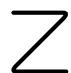
\includegraphics[keepaspectratio]{images/part002_ecaa53ed.jpg}}

\[
\int_ {n \pi} ^ {(n + 1) \pi} \frac {\sin^ {2} t}{t} d t \geqslant \frac {1}{(n + 1) \pi} \int_ {0} ^ {\pi} \sin^ {2} t d t \geqslant \frac {1}{2} \int_ {n + 1} ^ {n + 2} \frac {d t}{t},
\]

由此得

\[
\int_ {\pi} ^ {n \pi} \frac {\sin^ {2} t}{t} d t \geqslant \frac {1}{2} \int_ {2} ^ {n + 1} \frac {d t}{t}
\]

而积分 \(\int_{1}^{+\infty} dt / t\) 为无穷，尽管 \(\int_{\frac{\pi}{2}}^{x} g(t) dt = -\cos x\) 保持有界（参见 V, p.~260, exerc. 4）。

\subsection{比较关系的求导}

\pandocbounded{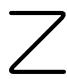
\includegraphics[keepaspectratio]{images/part002_390c97e1.jpg}}

命题 1 (V, p.~228) 与命题 6 (V, p.~230) 没有逆命题：两个函数之间的比较关系 \(\mathbf{f} \preccurlyeq g\) 、 \(\mathbf{f} \ll g\) 、 \(\mathbf{f} \sim \mathbf{c}g\) 的存在（这两个函数在 \(+\infty\) 的一个邻域上可导）并不蕴含它们的导数之间有同样的比较关系，即使对实单调函数 \(f\) 与 \(g\) 亦然。

例如，函数 \(x^{2} + x\sin x + \cos x\) 是单调的且等价于 \(x^{2}\) ，但它的导数 \(x(2 + \cos x)\) 不等价于 \(2x\) 。

另一方面，当先验地假设所考虑函数的导数是可比较的 (V, p.~217) 时，可以导出比较关系。一般地，我们将说定义在区间 \([a, +\infty]\) 上的两个实函数 f 与 g 在 \(+\infty\) 的一个邻域上是 k 阶可比较的，如果在 \(+\infty\) 的一个邻域上，它们各自除在一个可数集的点处外都有规则的 \(k^{th}\) 导数，并且在这个邻域上 \(f^{(k)}\) 与 \(g^{(k)}\) 具有常号（在其有定义的集上）且是可比较的。

我们约定称两个可比较的实函数（V, p.~217）为 0 阶可比较的。

命题 7. 若两个实函数 \(f, g\) 是 1 阶可比较的，则它们是可比较的；此外，关系 \(f \ll g\) （相应地， \(f \sim cg\) ， \(c\) 为常数）蕴含 \(f' \ll g'\) （相应地， \(f' \sim cg'\) ），除非 \(g\) 等价于一个非零常数。

现在，由于 \(f'\) 与 \(g'\) 在一个区间 \([x_0, +\infty[\) 上具有常号， \(f\) 与 \(g\) 都在这个区间上单调，故当 \(x\) 趋于 \(+\infty\) 时趋于一个有限或无穷的极限。显然， \(f\) 与 \(g\) 当 \(x\) 趋于 \(+\infty\) 时是可比较的（若这两个极限之一有限且 \(\neq 0\) ，或者一个为零而另一个为无穷）。若 \(f\) 与 \(g\) 都趋于 0，可以写 \(f(x) = -\int_x^{+\infty} f'(t) dt\) ， \(g(x) = -\int_x^{+\infty} g'(t) dt\) ；由于 \(f'\) 与 \(g'\) 可比较， \(f\) 与 \(g\) 亦然，且 \(f\) 与 \(g\) 之间的比较关系等同于 \(f'\) 与 \(g'\) 之间的比较关系（由 V, p.~20 的命题 6）。类似地，若 \(f\) 与 \(g\) 都有一个无穷极限，则有 \(f(x) = f(x_0) + \int_{x_0}^x f'(t) dt\) ， \(g(x) = g(x_0) + \int_{x_0}^x g'(t) dt\) ；V, p.~230 的命题 6 仍然表明 \(f\) 与 \(g\) 可比较，且 \(f\) 与 \(g\) 之间的比较关系等同于 \(f'\) 与 \(g'\) 之间的比较关系。为完成证明，剩下考虑 \(g\) 趋于 \(\pm \infty\) 而 \(f\) 趋于一个常数的情形；这时不可能有 \(f' \succcurlyeq g'\) ，因为那样由 V, p.~218 的命题 1 将可推出积分 \(\int_{x_0}^{+\infty} g'(t) dt\) 收敛；由于已假设 \(f'\) 与 \(g'\) 可比较，必有 \(f' \ll g'\) 。

推论. 若两个实函数 \(f, g\) 是 \(k \geqslant 1\) 阶可比较的，则它们是 \(p\) 阶可比较的（对 \(0 \leqslant p \leqslant k\) ）；此外，关系 \(f \ll g\) （相应地， \(f \sim cg\) ）蕴含 \(f^{(k)} \ll g^{(k)}\) （相应地， \(f^{(k)} \sim cg^{(k)}\) ），除非诸导数 \(g^{(p)}\) 之一（ \(0 \leqslant p \leqslant k - 1\) ）等价于一个常数 \(\neq 0\) 。

事实上，由于 \(f^{(k)}\) 与 \(g^{(k)}\) 在一个区间 \([x_0, +\infty[\) 上具有常号，由此得出 \(f^{(k-1)}\) 与 \(g^{(k-1)}\) 在这个区间上单调，故在 \(+\infty\) 的一个邻域上具有常号；此外，V, p.~232 的命题 7 表明 \(f^{(k-1)}\) 与 \(g^{(k-1)}\) 可比较，于是推论由递归地应用命题 7 而得。

注. 1) 命题 7 中对 \(g\) 的限制是本质的。例如，有 \(\frac{1}{x} \ll 1 + \frac{1}{x}\) ，尽管两边的导数是等价的；类似地 \(1 + \frac{1}{x} \sim 1 + \frac{1}{x^2}\) ，但 \(1 / x^2 \gg 2 / x^3\) 。

\begin{enumerate}
\def\labelenumi{\arabic{enumi})}
\setcounter{enumi}{1}
\item
  尽管 \(f\) 与 \(g\) 是 \(k\) 阶可比较的，一个函数 \(f_{1}\) （等价于 \(f\) 的）不必是 \(k\) 阶可比较的（与 \(g\) ）；但若假设 \(f_{1}\) 是 \(k\) 阶可比较的（与 \(f\) ），且诸导数 \(f^{(p)}\) （ \(0 \leqslant p \leqslant k - 1\) ）无一等价于一个非零常数，则它将是如此。
\item
  若 f 与 g 是 k 阶可比较的，这对 hf 与 hg 未必成立，即使对像 \(h(x) = x\) 这样简单的单调函数 h 亦然 (V, p.~260, exerc. 3)；同样，1/f 与 1/g 也不必然是 k 阶可比较的 (V, p.~259, exerc. 1)。
\end{enumerate}

\subsection{原函数的主部}

设 \(f\) 是一个规则实函数， \(\neq 0\) 且在一个区间 \([a, +\infty[\) 上具有常号；下面的命题使我们在某些情形能够得到原函数 \(\int_{x}^{+\infty} f(t) dt\) 的主部（若 \(\int_{a}^{+\infty} f(t) dt\) 收敛），以及原函数 \(\int_{a}^{x} f(t) dt\) 的主部（若 \(\int_{a}^{+\infty} f(t) dt\) 为无穷）：

命题 8. 置 \(\mathrm{F}(x) = \int_{x}^{+\infty} f(t) dt\) （若 \(\int_{a}^{+\infty} f(t) dt\) 收敛），而置 \(\mathrm{F}(x) = \int_{a}^{x} f(t) dt\) （若 \(\int_{a}^{+\infty} f(t) dt\) 为无穷）。设 \(\log |f|\) 与 \(\log x\) 是 1 阶可比较的。

\(1^{\circ}\) 若 \(f\) 是有限阶 \(\mu \neq -1\) 的（相对于 \(x\) ），则有

\[
\mathrm{F} (x) \sim \frac {1}{| \mu + 1 |} x f (x).\tag{1}
\]

\(2^{\circ}\) 若 \(f\) 相对于 \(x\) 是无穷阶的，且 \(f / f'\) 与 \(x\) 是 1 阶可比较的，则有

\[
\mathrm{F} (x) \sim \frac {(f (x)) ^ {2}}{| f ^ {\prime} (x) |}.\tag{2}
\]

应当注意，假设蕴含 \(f(x)\) 相对于 \(x\) 有确定的阶 (V, p.~219)。

\(1^{\circ}\) 若 \(f\) 是 \(\mu \neq 0\) 阶的（相对于 \(x\) ），则有 \(\log |f| \sim \mu \log x\) ，于是，由于 \(\log |f|\) 与 \(\log x\) 是 1 阶可比较的，由 V, p.~232 的命题 7 有 \(f'/f \sim\) \(\mu/x\) ，由此 \(xf' \sim \mu f\) 。若 \(\mu > -1\) ，则有 \(f(x) \gg x^{\mu-\varepsilon}\) （对每个 \(\varepsilon > 0\) ），从而 (V, p.~229, prop. 2) 积分 \(\int_{a}^{+\infty} f(t) dt\) 为无穷。可以写 \(F(x) = \int_{a}^{x} f(t) dt = xf(x) - af(a) - \int_{a}^{x} tf'(t) dt\) ，由此再次得到

\[
\int_ {a} ^ {x} \left(f (t) + t f ^ {\prime} (t)\right) d t = x f (x) - a f (a);
\]

由于 \(\mu \neq -1\) ，有 \(f(x) + xf'(x) \sim (\mu + 1)f(x)\) ，故 (V, p.~230, prop. 6)

\[
\int_ {a} ^ {x} \left(f (t) + t f ^ {\prime} (t)\right) d t \sim (\mu + 1) \mathrm{F} (x),
\]

这就在这种情形证明了 (1)。若 \(\mu = 0\) ，同样有 \(xf'(x) \ll f(x)\) ，它再次给出 \(f(x) + xf'(x) \sim f(x)\) 。当 \(\mu < -1\) 时论证类似（在 \(\int_{a}^{+\infty} f(t) dt\) 收敛的情形）。

\(2^{\circ}\) 若 \(f\) 是 \(+\infty\) 阶的（相对于 \(x\) ），则有 \(\log |f| \gg \log x\) ，故 (V, p.~232, prop. 7) \(f'/f \gg 1/x\) ，或者再令 \(g(x) = f(x)/f'(x)\) ，有 \(g(x) \ll x\) ；此外，由于 \(f(x) \gg x^{\alpha}\) （对每个 \(\alpha > 0\) ），积分 \(\int_{a}^{+\infty} f(t) dt\) 为无穷。可以写

\[
\mathrm{F} (x) = \int_ {a} ^ {x} f (t) d t = \int_ {a} ^ {x} g (t) f ^ {\prime} (t) d t = g (x) f (x) - g (a) f (a) - \int_ {a} ^ {x} f (t) g ^ {\prime} (t) d t;
\]

由于 \(g\) 与 \(x\) 是 1 阶可比较的，从关系 \(g(x) \ll x\) 可推出 (V, p.~232, prop. 7) \(g'(x) \ll 1\) ，从而 \(fg' \ll f\) ，于是 (V, p.~230, prop.6)

\[
\int_ {a} ^ {x} f (t) g ^ {\prime} (t) d t \ll \mathrm{F} (x),
\]

这就建立了关系式 (2)。当 \(f\) 是 \(-\infty\) 阶的（相对于 \(x\) ）时证明类似（在 \(\int_{a}^{+\infty} f(t) dt\) 收敛的情形）。

设 E 是一个比较尺度（对趋于 \(+\infty\) 的实 x 而言），由在 \(+\infty\) 的一个邻域上具有常号的非零实函数组成，使得 \(x \in E\) ，且 E 中两个函数的乘积与商仍属于 E (V, p.~221 and p.~224)。若一个在 \(+\infty\) 的一个邻域上具有常号的规则函数 f 相对于 E 有主部 cg，则 \(\int_{x}^{+\infty} f(t) dt\) （相应地， \(\int_{a}^{x} f(t) dt\) ，视情形而定）将等价于 \(c \int_{x}^{+\infty} g(t) dt\) （相应地， \(c \int_{a}^{x} g(t) dt\) ）；若函数 g 满足 V, p.~233 的命题 8 的假设，且（当 V, p.~233 的公式 (2) 适用时）知道 \(g'\) 相对于 E 的一个主部，则由此将有 \(\int_{x}^{+\infty} f(t) dt\) （相应地， \(\int_{a}^{x} f(t) dt\) ）相对于 E 的一个主部。

例. 1) 函数 \(1 / \log x\) 相对于 \(x\) 是 0 阶的且满足 V, p.~233 的命题 8 的条件；于是

\[
\int_ {a} ^ {x} \frac {d t}{\log t} \sim \frac {x}{\log x}.
\]

\begin{enumerate}
\def\labelenumi{\arabic{enumi})}
\setcounter{enumi}{1}
\tightlist
\item
  函数 \(e^{x^2}\) 是 \(+\infty\) 阶的（相对于 \(x\) ）且满足命题 8 的条件，故
\end{enumerate}

\[
\int_ {a} ^ {x} e ^ {t ^ {2}} d t \sim \frac {1}{2 x} e ^ {x ^ {2}}.
\]

在附录 (V, p.~252) 中我们将定义一类函数，对它们命题 7 与命题 8 总是适用的。

注. 命题 8 不直接应用于一个函数 \(f\) （ \(-1\) 阶的，相对于 \(x\) ）。但这时可以写 \(f(x) = f_1(x) / x\) ，其中 \(f_1\) 相对于 \(x\) 是 0 阶的。例如设 \(\int_{a}^{+\infty} f(t) dt\) 为无穷；则

\[
\mathrm{F} (x) = \int_ {a} ^ {x} f (t) d t = \int_ {a} ^ {x} \frac {1}{t} f _ {1} (t) d t = \int_ {\log a} ^ {\log x} f _ {1} \left(e ^ {u}\right) d u.
\]

若函数 \(f_{1}(e^{y})\) 满足命题 8 的假设且有一个 \(\neq -1\) 的阶（相对于 \(y\) ）（也就是说，若 \(f_{1}(x)\) 有一个 \(\neq -1\) 的阶（相对于 \(\log x\) ）），则公式 (1) 与 (2) 仍能使我们得到 \(F(x)\) 的一个主部。例如，设 \(f(x) = \frac{\exp(\sqrt{\log x})}{x\log x}\) ；由于 \(\exp(\sqrt{\log x})\) 相对于 \(x\) 是 0 阶的， \(f\) 是 \(-1\) 阶的；这里有 \(f_{1}(e^{y}) = e^{\sqrt{y}} / y\) ，且这个函数是 \(+\infty\) 阶的（相对于 \(y\) ）；命题 8 适用并给出 \(\int_{\alpha}^{y} e^{\sqrt{u}} / u du \sim 2e^{\sqrt{y}} / \sqrt{y}\) ；回到变量 \(x\) ，我们有 \(\int_{a}^{x} \frac{\exp(\sqrt{\log t})}{t\log t} dt \sim \frac{2\exp(\sqrt{\log x})}{\sqrt{\log x}}\) 。

\subsection{原函数的渐近展开}

设 E 是 \(+\infty\) 的一个邻域上的一个比较尺度，由 \(\neq 0\) 的、在 \(+\infty\) 的一个邻域上具有常号的实函数组成；设 f 是定义在一个区间 \([a, +\infty[\) 上的规则向量函数，取值于一个完备赋范空间 E 中，容许一个渐近展开

\[
\mathbf {f} = \sum_ {\lambda \leqslant \alpha} \mathbf {a} _ {\lambda} g _ {\lambda} + \mathbf {r} _ {\alpha}
\]

（精确到 \(g_{\alpha}\) ，相对于 E）。进一步假设每个原函数 \(\int_{a}^{x} g(t) dt\) （函数 \(g \in E\) 的）相对于 E 容许一个渐近展开。在这些情形下我们将看到，可以得到 \(\mathbf{F}(x) = \int_{a}^{x} \mathbf{f}(t) dt\) 相对于 E 的一个渐近展开。我们区分两种情形：

\(1^{\circ}\int_{a}^{+\infty}g_{\alpha}(t)dt\) 为无穷；则有 \(\int_{a}^{x}\mathbf{r}_{\alpha}(t)dt\ll \int_{a}^{x}g_{\alpha}(t)dt\) (V,p.230, prop. 6)；由假设可以得到 \(\sum_{\lambda \leqslant \alpha}\mathbf{a}_{\lambda}\int_{a}^{x}g_{\lambda}(t)dt\) 的一个渐近展开

（精确到某个 \(g_{\rho}\) ）(V, p.~222)；若 \(cg_{\sigma}\) 是 \(\int_{a}^{x} g_{\alpha}(t) dt\) 的主部，则由此将有 \(\int_{a}^{x} \mathbf{f}(t) dt\) 的一个精确到 \(g_{\min(\rho, \sigma)}\) 的渐近展开，其所有项的范数不定递增。

\(2^{\circ}\int_{a}^{+\infty}g_{\alpha}(t)dt\) 收敛；设 \(\beta\) 是指标 \(\lambda \leqslant \alpha\) 中最小的使 \(\mathbf{a}_{\lambda}\neq 0\) 且使 \(\int_{a}^{+\infty}g_{\lambda}(t)dt\) 收敛者；积分

\[
\mathbf {C} = \int_ {a} ^ {+ \infty} \left(\mathbf {f} (t) - \sum_ {\lambda <   \beta} \mathbf {a} _ {\lambda} g _ {\lambda} (t)\right) d t
\]

这时收敛，且可以写

\[
\mathbf {F} (x) = \sum_ {\lambda <   \beta} \mathbf {a} _ {\lambda} \int_ {a} ^ {x} g _ {\lambda} (t) d t + \mathbf {C} - \sum_ {\beta \leqslant \lambda \leqslant \alpha} \mathbf {a} _ {\lambda} \int_ {x} ^ {+ \infty} g _ {\lambda} (t) d t - \int_ {x} ^ {+ \infty} \mathbf {r} _ {\alpha} (t) d t.
\]

则 \(\int_{x}^{+\infty}\mathbf{r}_{\alpha}(t)dt\ll \int_{x}^{+\infty}g_{\alpha}(t)dt\) ；若 \(cg_{\sigma}\) 是 \(\int_{x}^{+\infty}g_{\alpha}(t)dt\) 的主部，且若有

\[
\sum_ {\lambda <   \beta} \mathbf {a} _ {\lambda} \int_ {a} ^ {x} g _ {\lambda} (t) d t + \mathbf {C} - \sum_ {\beta \leqslant \lambda \leqslant \alpha} \mathbf {a} _ {\lambda} \int_ {x} ^ {+ \infty} g _ {\lambda} (t) d t
\]

的一个渐近展开（精确到 \(g_{\rho}\) ），则由此将有 \(\mathbf{F}\) 的一个精确到 \(g_{\min(\rho, \sigma)}\) 的渐近展开。

于是问题归结为求 E 中函数的原函数相对于 E 的渐近展开。我们已经看到，在某些关于 E 的假设下，V, p.~233 的命题 8 如何给出这种原函数的主部。此外，命题 8 的证明给出 V, p.~233 的公式 (1) （相应地， (2)）两边之差的表达式，其形式为函数 \(\frac{1}{|\mu+1|}\left(xf'(x)+f(x)\right)-f(x)\) （相应地， \(f(x)g'(x)\) ，其中 \(g=f/f'\) ）的一个原函数；在构成这个新原函数的主部（作为 (1) （相应地， (2)）右边的一个渐近展开）时，就得到所求展开的右边（参见 V, p.~247-255）。

例. 1) 设 \(f(x) = 1 / \log x\) （ \(x > 1\) ）；我们已经看到 \(\int_{a}^{x} dt / \log t \sim x / \log x\) ，且差 \(\int_{a}^{x} \frac{dt}{\log t} - \frac{x}{\log x}\) 是 \(1 / (\log x)^2\) 的一个原函数；对这个函数可再次应用命题 8，从而得到 \(\int_{a}^{x} dt / (\log t)^2 \sim x / (\log x)^2\) 。由递归于是得到展开

\[
\begin{array}{l} \int_ {a} ^ {x} \frac {d t}{\log t} = \frac {x}{\log x} + \frac {x}{(\log x) ^ {2}} \\ \qquad + \frac {2 x}{(\log x) ^ {3}} + \dots + (n - 1)! \frac {x}{(\log x) ^ {n}} + o \left(\frac {x}{(\log x) ^ {n}}\right). \end{array}
\]

注意，不论 n 为何，这个展开的所有项都随 x 趋于 \(+\infty\) 。

\begin{enumerate}
\def\labelenumi{\arabic{enumi})}
\setcounter{enumi}{1}
\tightlist
\item
  设 \(f(x) = \frac{e^x}{x^2 + 1}\) ；可以写 \(f(x) = \frac{e^x}{x^2} - \frac{e^x}{x^4} + o_1\left(\frac{e^x}{x^4}\right)\) 。命题 8 给出展开
\end{enumerate}

\[
\int_ {a} ^ {x} \frac {e ^ {t}}{t ^ {2}} d t = \frac {e ^ {x}}{x ^ {2}} + \frac {2 e ^ {x}}{x ^ {3}} + \frac {6 e ^ {x}}{x ^ {4}} + o _ {2} \left(\frac {e ^ {x}}{x ^ {4}}\right), \quad \int_ {a} ^ {x} \frac {e ^ {t}}{t ^ {4}} d t = \frac {e ^ {x}}{x ^ {4}} + o _ {3} \left(\frac {e ^ {x}}{x ^ {4}}\right)
\]

由此，把两式相加，

\[
\int_ {a} ^ {x} \frac {e ^ {t}}{t ^ {2} + 1} d t = \frac {e ^ {x}}{x ^ {2}} + 2 \frac {e ^ {x}}{x ^ {3}} + 5 \frac {e ^ {x}}{x ^ {4}} + o _ {4} \left(\frac {e ^ {x}}{x ^ {4}}\right).
\]

\section{应用于正项级数}

\subsection{正项级数的收敛判别法}

在本节中，我们把（滥用语言的说法）这样的实项级数 \((u_{n})\) ：其项 \(u_{n} \geqslant 0\) 从 \(n\) 的某个特定值起成立，理解为正项级数。我们关于这类级数所说的一切，通过改变符号，立即可以推广到各项都 \(\leqslant 0\) （从 \(n\) 的某个特定值起）的级数。我们已经看到 (II, p.~64, 例 3)，对点的每个序列 \((\mathbf{u}_n)_{n\geqslant 1}\) （取值于赋范空间 \(E\) ），可以关联一个阶梯函数 \(\mathbf{u}\) ，它定义在 \([1, +\infty[\) 上，由条件 \(\mathbf{u}(x) = \mathbf{u}_n\) （对 \(n\leqslant x < n + 1\) ）确定：这时级数 \((\mathbf{u}_n)\) 收敛当且仅当积分 \(\int_1^{+\infty}\mathbf{u}(t)dt\) 收敛。

设 \((u_{n})\) 与 \((v_{n})\) 是两个正项级数，u 与 v 是相应的阶梯函数：关系 \(u_{n} \leqslant v_{n}\) （对 \(n \geqslant n_{0}\) ）等价于 \(u(x) \leqslant v(x)\) （对 \(x \geqslant n_{0}\) ）。于是关系 \(u_{n} \preccurlyeq v_{n}, u_{n} \prec v_{n}, u_{n} \sim v_{n}\) 中的每一个分别等价于 \(u(x) \preccurlyeq v(x), u(x) \prec v(x)\) 与 \(u(x) \sim v(x)\) ；这一注记使我们能把命题 1 (V, p.~228) 与命题 6 (V, p.~230) 表述如下：

命题 1. 设 \((u_{n})\) 与 \((v_{n})\) 是两个正项级数。若 \(u_{n} \preccurlyeq v_{n}\) 且级数 \((v_{n})\) 收敛，则 \((u_{n})\) 收敛；若 \(u_{n} \succcurlyeq v_{n}\) 且 \(\sum_{n=1}^{\infty} v_{n} = +\infty\) ，则 \(\sum_{n=1}^{\infty} u_{n} = +\infty\) 。

命题 2. 设 \((u_{n})\) 与 \((v_{n})\) 是两个正项级数：

\(1^{\circ}\) 若级数 \((v_{n})\) 收敛，则关系 \(u_{n} \ll v_{n}\) （相应地， \(u_{n} \sim v_{n}\) ）蕴含 \(\sum_{p=n}^{\infty} u_{p} \ll \sum_{p=n}^{\infty} v_{p}\) （相应地， \(\sum_{p=n}^{\infty} u_{p} \sim \sum_{p=n}^{\infty} v_{p}\) ）。

\(2^{\circ}\) 若 \(\sum_{n=1}^{\infty} v_n = +\infty\) ，则关系 \(u_n \ll v_n\) （相应地， \(u_n \sim v_n\) ）蕴含 \(\sum_{p=1}^{n} u_p \ll \sum_{p=1}^{n} v_p\) （相应地， \(\sum_{p=1}^{n} u_p \sim \sum_{p=1}^{n} v_p\) ）。

在命题 1 中取比较级数 \((v_{n})\) 为通项形如 \(v_{n} = f(n)\) 的级数（其中 \(f\) 是一个 \(\geqslant 0\) 的函数，对每个实数 \(x > x_0\) 有定义且在区间 \([x_0, +\infty[\) 上递减），便得到方便的收敛判别法；事实上：

命题 3（柯西–麦克劳林判别法）. 若 \(f\) 是一个 \(\geqslant 0\) 且在 \([x_0, +\infty[\) 上递减的函数，则以 \(v_n = f(n)\) 为通项的级数收敛当且仅当积分 \(\int_{x_0}^{+\infty} f(t) dt\) 收敛。

为证明这一点，只需注意：若 v 是与级数 \((v_{n})\) 相关联的阶梯函数，则由于 f 递减， \(v(x+1) \leqslant f(x) \leqslant v(x)\) 对每个 \(x \geqslant x_{0}\) 成立；于是该命题是比较原理 (II, p.~66, prop. 3) 的推论。

由于出现在积分的对数收敛判别法 (V, p.~229, prop. 2、3 与 4) 中的函数在某个区间 \([x_{0}, +\infty[\) 上递减，应用 V, p.~237 的命题 1 与命题 3，就得到下列判别法：

命题 4（“0 阶对数判别法”）. 设 \((u_{n})\) 是正项级数；若 \(u_{n} \preccurlyeq n^{\mu}\) 对某个 \(\mu < -1\) 成立，则级数 \((u_{n})\) 收敛；若 \(u_{n} \succcurlyeq n^{\mu}\) 对某个 \(\mu \geqslant -1\) 成立，则级数 \((u_{n})\) 的和为无穷。

命题 5（“p 阶对数判别法”）. 设 \((u_{n})\) 是正项级数。若 \(u_{n} \preccurlyeq \frac{1}{nl_{1}(n)l_{2}(n)\ldots l_{p-1}(n)(l_{p}(n))^{\mu}}\) 对某个 \(\mu > 1\) 成立，则级数 \((u_{n})\) 收敛；若 \(u_{n} \succcurlyeq \frac{1}{nl_{1}(n)l_{2}(n)\ldots l_{p-1}(n)(l_{p}(n))^{\mu}}\) 对某个 \(\mu \leqslant 1\) 成立，则级数 \((u_{n})\) 的和为无穷。

若 \(0 \leqslant q < 1\) ，则 \(q^n \preccurlyeq n^{-\mu}\) 对任何 \(\mu > 0\) 成立；再应用 0 阶对数判别法便证明了几何级数 \(\sum_{n=0}^{\infty} q^n\) 对 \(|q| < 1\) 收敛 (Gen.~Top., IV, p.~364)。若在命题 1 中取 \(v_n = q^n\) ，就得到一个可以写成如下形式的判别法（“柯西判别法”）：设 \((u_n)\) 是正项级数；若 \(\limsup_{n \to \infty} (u_n)^{1/n} < 1\) ，则级数 \((u_n)\) 收敛；若 \(\limsup_{n \to \infty} (u_n)^{1/n} > 1\) ，则级数 \((u_n)\) 的和为无穷。事实上，若 \(\limsup_{n \to \infty} (u_n)^{1/n} = a < 1\) ，则 \(u_n \preccurlyeq q^n\) 对每个 \(q\) （使 \(a < q < 1\) ）成立。反之，若 \(\limsup_{n \to \infty} (u_n)^{1/n} = a > 1\) ，则 \(u_n \geqslant q^n > 1\) 对无穷多个 \(n\) 的值成立（对任何 \(q\) ，满足 \(1 < q < a\) ）；由于 \(u_n\) 不趋于 0，有 \(\sum_{n=1}^{\infty} u_n = +\infty\) 。

这个判别法在整级数理论（我们将在以后研究它）中非常有用；但即便如此，它仍不能判定级数 \((1/n^{\alpha})\) 的收敛性，换句话说，它的应用范围比对数判别法狭窄得多。

\subsection{级数部分和的渐近展开}

对实变量 \(x\) （趋于 \(+\infty\) ），设 \(\mathcal{E}\) 是一个比较尺度，由这样的函数组成：其中每个函数都在整个区间 \([x_0, +\infty[\) （随函数而定）上有定义，且在该区间上 \(\geqslant 0\) 。设 \((\mathbf{u}_n)\) 是各项都属于完备赋范空间 \(E\) 的级数，使得 \(\mathbf{u}_n\) 有精确到 \(g_\alpha\) 的渐近展开，它相对于尺度 \(\mathcal{E}'\) （由 \(\mathbf{N}\) 上的、来自 \(\mathcal{E}\) 中函数的限制组成）：

\[
\mathbf {u} _ {n} = \sum_ {\lambda \leqslant \alpha} \mathbf {a} _ {\lambda} g _ {\lambda} (n) + \mathbf {r} _ {\alpha} (n).
\]

假设每个部分和 \(\sum_{m=1}^{n} g(m)\) （其中 \(g \in \mathcal{E}\) ）都有关于 \(\mathcal{E}'\) 的渐近展开。于是可以得到 \(\mathbf{s}_n = \sum_{m=1}^{n} \mathbf{u}_m\) 关于 \(\mathcal{E}'\) 的渐近展开；我们仍然区分两种情形：

\(1^{\circ}\sum_{n = 1}^{\infty}g_{\alpha}(n) = +\infty .\) 这时 (V,p.237,prop.2) 有 \(\sum_{m = 1}^{n}\mathbf{r}_{\alpha}(m)\ll \sum_{m = 1}^{n}g_{\alpha}(m);\)

根据假设，可以得到

\[
\sum_ {\lambda \leqslant \alpha} \mathbf {a} _ {\lambda} \left(\sum_ {m = 1} ^ {n} g (m)\right)
\]

(V, p.~222) 到某个精确度 \(g_{\sigma}\) 的渐近展开；若 \(cg_{\sigma}(n)\) 是 \(\sum_{m=1}^{n} g_{\alpha}(m)\) 的主部，则将有 \(\mathbf{s}_n\) 的精确到 \(g_{\min(\rho, \sigma)}\) 的渐近展开。

\(2^{\circ}\sum_{n = 1}^{\infty}g_{\alpha}(n)\) 收敛；这时设 \(\beta\) 是指标 \(\lambda \leqslant \alpha\) 中最小的一个，它使 \(\mathbf{a}_{\lambda}\neq 0\) 且使 \(\sum_{n = 1}^{\infty}g_{\lambda}(n)\) 收敛；则级数

\[
\mathbf {C} = \sum_ {n = 1} ^ {\infty} \left(\mathbf {u} _ {n} - \sum_ {\lambda <   \beta} \mathbf {a} _ {\lambda} g _ {\lambda} (n)\right)
\]

绝对收敛，并且可以写

\[
\mathbf {s} _ {n} = \sum_ {\lambda <   \beta} \mathbf {a} _ {\lambda} \left(\sum_ {m = 1} ^ {n} g _ {\lambda} (m)\right) + \mathbf {C} - \sum_ {\beta \leqslant \lambda \leqslant \alpha} \mathbf {a} _ {\lambda} \left(\sum_ {m = n + 1} ^ {\infty} g _ {\lambda} (m)\right) - \sum_ {m = n + 1} ^ {\infty} \mathbf {r} _ {\alpha} (m).
\]

此外，有 \(\sum_{m=n+1}^{\infty}\mathbf{r}_{\alpha}(m)\ll\sum_{m=n+1}^{\infty}g_{\alpha}(m)\) ；若 \(cg_{\sigma}(n)\) 是 \(\sum_{m=n+1}^{\infty}g_{\alpha}(m)\) 的主部，且若已有

\[
\sum_ {\lambda <   \beta} \mathbf {a} _ {\lambda} \left(\sum_ {m = 1} ^ {n} g _ {\lambda} (m)\right) + \mathbf {C} - \sum_ {\beta \leqslant \lambda \leqslant \alpha} \mathbf {a} _ {\lambda} \left(\sum_ {m = n + 1} ^ {\infty} g _ {\lambda} (m)\right)
\]

到精确度 \(g_{\rho}\) 的渐近展开，便由此得到 \(s_{n}\) 的精确到 \(g_{\min(\rho,\sigma)}\) 的渐近展开。于是问题归结为级数 \((g(n))\) （其中 \(g \in E\) ）的特殊情形。我们将看到，在某些条件之下，如何能直接得到 \(s_{n} = \sum_{m=1}^{n} g(m)\) 的主部（当 \(\sum_{n=1}^{\infty} g(n) = +\infty\) 时）或 \(r_{n} = \sum_{m=n+1}^{\infty} g(m)\) 的主部（当 \(\sum_{n=1}^{n} g(n) < +\infty\) 时）。

命题 6. 设 \(g\) 是一个实函数， \(>0\) 且单调，定义在区间 \([x_0, +\infty[\) 上（其中 \(x_0 \leqslant 1\) ），且使 \(\log g\) 与 \(x\) 1 阶可比较。

\(1^{\circ}\) 若 \(g\) 相对于 \(e^{x}\) 是无穷阶的，则有

\[
s _ {n} = \sum_ {m = 1} ^ {n} g (m) \sim g (n) \quad i f \quad \sum_ {n = 1} ^ {\infty} g (n) = + \infty ;\tag{1}
\]

\[
r _ {n} = \sum_ {m = n + 1} ^ {\infty} g (m) \sim g (n + 1) \quad i f \quad \sum_ {n = 1} ^ {\infty} g (n) <   + \infty .\tag{2}
\]

\(2^{\circ}\) 若 \(g\) 有有限阶 \(\mu\) （相对于 \(e^{x}\) ），则有

\[
s _ {n} = \sum_ {m = 1} ^ {n} g (m) \sim \frac {\mu}{1 - e ^ {- \mu}} \int_ {x _ {0}} ^ {n} g (t) d t \quad i f \quad \sum_ {n = 1} ^ {\infty} g (n) = + \infty ;\tag{3}
\]

\[
r _ {n} = \sum_ {m = n + 1} ^ {\infty} g (m) \sim \frac {\mu}{1 - e ^ {- \mu}} \int_ {n} ^ {\infty} g (t) d t \quad i f \quad \sum_ {n = 1} ^ {\infty} g (n) <   + \infty\tag{4}
\]

（数 \(\frac{\mu}{1 - e^{-\mu}}\) 在 (3) 与 (4) 中当 \(\mu = 0\) 时应换成 1）。

\(1^{\circ}\) 若 \(g\) 的阶为 \(+\infty\) （相对于 \(e^{x}\) ），则有 \(\log g \gg x\) ，从而按假设有 \(g' / g \gg 1\) ，即 \(g' \gg g\) ；因此 \(g\) 递增并趋于 \(+\infty\) （随 \(x\) ），从而 \(\sum_{n=1}^{\infty} g(n) = +\infty\) 。若 \(u\) 是与级数 \((g(n))\) 相关联的阶梯函数 (V, p.~237)，则 \(u(x) \leqslant g(x)\) 从 \(x\) 的某个值起成立，故 \(u \preccurlyeq g\) ，因而

\[
s _ {n - 1} = \int_ {1} ^ {n} u (t) d t \preccurlyeq \int_ {1} ^ {n} g (t) d t \prec \prec \int_ {1} ^ {n} g ^ {\prime} (t) d t \sim g (n);
\]

由于 \(s_n = s_{n-1} + g(n)\) ，有 \(s_n \sim g(n)\) 。当 \(g\) 的阶为 \(-\infty\) （相对于 \(e^x\) ）时，证明类似；这样便得到公式 (2)。

\(2^{\circ}\) 若 \(g\) 有有限阶 \(\mu\) （相对于 \(e^{x}\) ），则可写 \(g(x) = e^{\mu x}h(x)\) ，其中 \(h\) 相对于 \(e^{x}\) 是 0 阶的；此外，按假设， \(\log g \sim \mu x\) （对 \(\mu \neq 0\) ； \(\log g \prec x\) 对 \(\mu = 0\) ）蕴含 \(h' \prec h\) 。先设 \(\sum_{n=1}^{\infty} g(n) = +\infty\) （这蕴含 \(\mu \geqslant 0\) ；当 \(\mu > 0\) 时逆命题总成立，因为这时 \(g(x)\) 趋于 \(+\infty\) （随 \(x\) ））；我们来求 \(\int_{n-1}^{n} g(t) dt\) 的主部。可以写

\[
\begin{array}{l} \int_ {n - 1} ^ {n} g (t) d t = \int_ {n - 1} ^ {n} e ^ {\mu t} h (t) d t \\ \qquad = h (n) \int_ {n - 1} ^ {n} e ^ {\mu t} d t + \int_ {n - 1} ^ {n} e ^ {\mu t} \big (h (t) - h (n) \big) d t \\ \qquad = \frac {1 - e ^ {- \mu}}{\mu} g (n) + \int_ {n - 1} ^ {n} e ^ {\mu t} \big (h (t) - h (n) \big) d t. \end{array}
\]

现在，关系 \(h^{\prime} \ll h\) 蕴含：对每个 \(\varepsilon > 0\) ，存在 \(n_{0}\) ，使关系 \(x \geqslant n_{0}\) 蕴含 \(\left|h'(x)/h(x)\right| \leqslant \varepsilon\) ；由中值定理推出 \(-\varepsilon \leqslant \log |h(t)/h(n)| \leqslant \varepsilon\) （对 \(n - 1 \leqslant t \leqslant n\) ，当 \(n \geqslant n_{0}\) 时），由此

\[
| h (t) - h (n) | \leqslant \left(e ^ {\varepsilon} - 1\right) h (n)
\]

从而

\[
\left| \int_ {n - 1} ^ {n} e ^ {\mu t} (h (t) - h (n)) d t \right| \leqslant (e ^ {\varepsilon} - 1) e ^ {\mu n} h (n) = (e ^ {\varepsilon} - 1) g (n)
\]

因为 \(e^{\mu t}\) 递增。由于 \(e^{\varepsilon} - 1\) 随 \(\varepsilon\) 变得任意小，可见可以写

\[
\int_ {n - 1} ^ {n} g (t) d t = \frac {1 - e ^ {- \mu}}{\mu} g (n) + o (g (n))
\]

（\(\left(\frac{1 - e^{-\mu}}{\mu}\right.\) 当 \(\mu = 0\) 时换成 1。于是该命题是 V, p.~237 的命题 2 的推论。当 \(\sum_{n=1}^{\infty} g(n)\) 有限时，论证类似。

反复应用 V, p.~239 的命题 6，有时便能得到 \(s_{n} = \sum_{m=1}^{n} g(m)\) 的渐近展开。首先设 g 的阶为 \(+\infty\) （相对于 \(e^{x}\) ）；对 p 的每个固定值，由命题 6 可以写

\[
s _ {n} = g (n) + g (n - 1) + \dots + g (n - p) + o (g (n - p))
\]

只需（关于 \(E'\) ）展开每个函数 \(g(n-k)\) （ \(0 \leqslant k \leqslant p\) ），并把展开的精确度限制到 \(g(n-p)\) 的主部，便得到 \(s_{n}\) 的展开。

例. 设 \(g(x) = x^{x} = \exp (x\log x)\) ，其阶为 \(+\infty\) （相对于 \(e^x\) ）。取 \(p = 2\) ，有

\[
(n - 1) \log (n - 1) = (n - 1) \log n - 1 + \frac {1}{2 n} + o \left(\frac {1}{n}\right)
\]

由此 (V, p.~225)

\[
(n - 1) ^ {n - 1} = \frac {1}{e} n ^ {n - 1} + \frac {1}{2 e} n ^ {n - 2} + o _ {1} (n ^ {n - 2})
\]

同理

\[
(n - 2) ^ {n - 2} = \frac {1}{e ^ {2}} n ^ {n - 2} + o _ {2} (n ^ {n - 2});
\]

因此

\[
s _ {n} = n ^ {n} + \frac {1}{e} n ^ {n - 1} + \left(\frac {1}{2 e} + \frac {1}{e ^ {2}}\right) n ^ {n - 2} + o _ {3} (n ^ {n - 2}).
\]

对 \(r_n\) ，当 \(g\) 的阶为 \(-\infty\) （相对于 \(e^x\) ）时，同样处理。

现在若 \(g\) 有有限阶 \(\mu\) （相对于 \(e^x\) ），且例如 \(\sum_{n=1}^{\infty} g(n) = +\infty\) ，则可以写

\[
s _ {n} = \frac {\mu}{1 - e ^ {- \mu}} \int_ {1} ^ {n} g (t) d t + \sum_ {m = 1} ^ {n} f _ {1} (m)
\]

其中 \(f_{1}(n) = g(n) - \frac{\mu}{1 - e^{-\mu}}\int_{1}^{n}g(t)dt \ll g(n)\) （由 V, p.~239 的命题 6）。若已有 \(cg_{1}(n)\) 作为 \(f_{1}(n)\) 关于 \(\mathcal{E}'\) 的主部，且若能对函数 \(g_{1}\) 再应用命题 6，则将得到与 \(\sum_{m=1}^{n}f_{1}(m)\) 等价的原函数（当 \(\sum_{n=1}^{\infty}g_{1}(n) = +\infty\) 时），而在相反的情形得到与 \(\sum_{m=n+1}^{\infty}f_{1}(m)\) 等价的原函数（在后一情形写 \(\sum_{m=1}^{n}f_{1}(m) = C - \sum_{m=n+1}^{\infty}f_{1}(m)\) ，其中 \(C = \sum_{n=1}^{\infty}f_{1}(n)\) ）。

这样逐步进行，最终可以把 \(s_{n}\) 表示成若干个原函数之和，其中每个原函数相对于前一个是可忽略的，外加一项相对于已写出的最后一个原函数仍为可忽略的项，最后还有一个常数（余项趋于 0 的情形）。然后只需关于 \(E'\) 展开所得到的每个原函数 (cf.~V, p.~235)。

例. 设 \(g(n) = \frac{1}{n}\) ；这时

\[
s _ {n} = \sum_ {m = 1} ^ {n} \frac {1}{m} \sim \int_ {1} ^ {n} \frac {d t}{t} = \log n
\]

继而

\[
\frac {1}{n} - (\log n - \log (n - 1)) \sim - \frac {1}{2 n ^ {2}}
\]

由此

\[
s _ {n} = \log n + \gamma + \frac {1}{2 n} + o \left(\frac {1}{n}\right).
\]

出现在这个公式中的常数 \(\gamma\) 在分析中扮演着重要角色 (cf.~chap.~VI 与 VII)；它称为欧拉常数；有

\[
\gamma = 0. 5 7 7   2 1 5   6 6 4 \dots
\]

精确到 \(1/10^{9}\) 。

我们将在 VI, p.~288 看到，欧拉–麦克劳林求和公式如何在最重要的情形给出 \(s_n\) （或 \(r_n\) ）的任意阶渐近展开。

\subsection{无穷乘积部分积的渐近展开}

我们知道 (Gen.~Top., V, p.~22 与 23)，以 \(1 + u_{n}\) （ \(u_{n} > -1\) ）为通项因子的无穷乘积收敛（相应地，交换收敛）的必要充分条件是：以 \(\log(1 + u_{n})\) 为通项的级数收敛（相应地，交换收敛），并且这时有关系

\[
\log \prod_ {n = 1} ^ {\infty} (1 + u _ {n}) = \sum_ {n = 1} ^ {\infty} \log (1 + u _ {n}).
\]

当无穷乘积收敛时，我们知道 \(u_{n}\) 趋于 0；于是 \(\log(1 + u_{n}) \sim u_{n}\) ；又我们知道，实数项级数交换收敛的必要充分条件是它绝对收敛 (Gen.~Top., IV, p.~372, prop. 5)；于是由命题 1 重新得到如下事实：以 \(1 + u_{n}\) 为通项因子的乘积交换收敛当且仅当以 \(u_{n}\) 为通项的级数绝对收敛 (Gen.~Top., IV, p.~368, th. 4)。

类似的论证适用于通项因子为复数 \(1 + u_{n}\) （ \(u_{n} \neq -1\) ）的无穷乘积。事实上，这样的乘积交换收敛的必要充分条件是 (Gen.~Top., VIII, p.~115, prop. 2)：以 \(|1 + u_{n}|\) 为通项因子的无穷乘积交换收敛，此外，若 \(\theta_{n}\) 是 \(1 + u_{n}\) 的辐角（取在 \(-\pi\) 与 \(+\pi\) 之间），则诸 \(\theta_{n}\) 所成的级数交换收敛。由于 \(u_{n}\) 趋于 0， \(\log(1 + u_{n})\) 从 n 的某个特定值起有定义 (III, p.~100)，且有

\[
\log (1 + u _ {n}) = \log | 1 + u _ {n} | + i \theta_ {n};
\]

于是，以 \(1 + u_{n}\) 为通项因子的乘积交换收敛的必要充分条件是：以 \(|\log(1 + u_{n})|\) 为通项的级数绝对收敛 (Gen.~Top., VII, p.~84, th. 1)；而 \(\log(1 + u_{n}) \sim u_{n}\) (I, p.~18, prop. 5)，故重新得到以 \(u_{n}\) 为通项的级数绝对收敛这一条件 (Gen.~Top., VIII, p.~116, th. 1)。

无穷乘积与实数项级数之间的关系有时使我们能得到部分积 \(p_{n} = \prod_{k=1}^{n}(1 + u_{k})\) 的渐近展开；只需有部分和 \(s_{n} = \sum_{k=1}^{n} \log(1 + u_{k})\) 的渐近展开，再展开 \(p_{n} = \exp(s_{n})\) 即可；于是问题归结为前面考察过的两个问题 (V, p.~238 与 p.~226)。

例：斯特林公式. 我们来求 \(n!\) 的渐近展开；这导致我们展开 \(s_n = \sum_{p=1}^{n} \log p\) ，然后展开 \(\exp(s_n)\) 。 \(n^{\circ} 2\) 的方法依次给出

\[
s _ {n} = \sum_ {p = 1} ^ {n} \log p \sim \int_ {1} ^ {n} \log t d t = n \log n - n + 1
\]

继而

\[
\log n - \int_ {n - 1} ^ {n} \log t d t = \log n - (n \log n - (n - 1) \log (n - 1) - 1) \sim \frac {1}{2 n}
\]

由此

\[
s _ {n} = n \log n - n + \frac {1}{2} \log n + o (\log n).
\]

然后

\[
\log n - \int_ {n - 1} ^ {n} \log t d t - \frac {1}{2} (\log n - \log (n - 1)) \sim - \frac {1}{1 2 n ^ {2}}
\]

由此

\[
s _ {n} = n \log n - n + \frac {1}{2} \log n + k + \frac {1}{1 2 n} + o _ {1} \left(\frac {1}{n}\right)
\]

（k 为常数）

最后由此推出 (V, p.~226)

\[
n! = e ^ {k} n ^ {n + 1 / 2} e ^ {- n} \left(1 + \frac {1}{1 2 n} + o _ {2} \left(\left(\frac {1}{n}\right)\right)\right).\tag{5}
\]

我们将在 VII, p.~322 证明 \(e^k = \sqrt{2\pi}\) 。公式 (5)（取 \(k\) 的这个值）称为斯特林公式。同样，对每个实数 \(a\) （非 \(>0\) 的整数），可以证明

\[
(a + 1) (a + 2) \dots (a + n) \sim \mathrm{K} (a) n ^ {n + a + \frac {1}{2}} e ^ {- n}.\tag{6}
\]

我们也将在 (VII, p.~18) 确定函数 \(\mathrm{K}(a)\) 。由公式 (5) 与 (6) 特别可推出

\[
\binom {a} {n} \sim (- 1) ^ {n}   \varphi (a)   n ^ {- a - 1}\tag{7}
\]

对每个实数 \(a\) （非 \(> 0\) 的整数）成立，其中 \(\varphi(a)\) 是 \(a\) 的一个函数，将在 VII, p.~322 明确给出。

\subsection{应用：正项级数的第二类收敛判别法}

我们经常遇到这样的级数 \((u_{n})\) ：从某项起 \(u_{n} > 0\) ，且 \(u_{n+1}/u_{n}\) 有一个容易确定的渐近展开。对这样的级数，拥有一些（称为第二类判别法的）判别法，使得仅从 \(u_{n+1}/u_{n}\) 的形状就能确定级数是否收敛，是很方便的。下面就是这样一个判别法：

命题 7（“拉阿贝判别法”）. 设 \((u_{n})\) 是从某项起各项 \textgreater{} 0 的级数。若从某个时刻起 \(u_{n+1}/u_{n} \leqslant 1 - \frac{\alpha}{n}\) （对某个 \(\alpha > 1\) ），则级数 \((u_{n})\) 收敛；若从某个时刻起有 \(u_{n+1}/u_{n} \geqslant 1 - \frac{1}{n}\) ，则级数 \((u_{n})\) 的和为无穷。

事实上，若 \(u_{n+1} / u_n \leqslant 1 - \frac{\alpha}{n}\) （其中 \(\alpha > 1\) ）对一切 \(n \geqslant n_0\) 成立，则有 \(u_n \preccurlyeq p_n = \prod_{k=n_0}^{n} \left(1 - \frac{\alpha}{k}\right)\) 。而 \(\log \left(1 - \frac{\alpha}{n}\right) = -\frac{\alpha}{n} - \frac{\alpha^2}{2n^2} + o\left(\frac{1}{n^2}\right)\) ，由此 \(\log p_n =\) \(-\alpha \log n + k + o(1/n) (k \text{ 为常数}), \text{ 且 } p_n \sim e^k \frac{1}{n^\alpha}; \text{ 由于 } \alpha > 1 \text{ 0 阶对数判别法足以完成证明。}\)

反之，若从某个时刻起有 \(u_{n + 1} / u_n \geqslant 1 - \frac{1}{n}\) ，则同样的计算证明 \(u_n \succcurlyeq \frac{1}{n}\) ，命题得证。

利用阶 \textgreater{} 0 的对数判别法，同样可以证明下列第二类判别法：

命题 8. 设 \((u_n)\) 是从某个时刻起各项 \(>0\) 的级数。若从某个时刻起有

\[
\frac {u _ {n + 1}}{u _ {n}} \leqslant 1 - \frac {1}{n} - \frac {1}{n l _ {1} (n)} - \dots - \frac {1}{n l _ {1} (n) l _ {2} (n) \dots l _ {p - 1} (n)} - \frac {\alpha}{n l _ {1} (n) l _ {2} (n) \dots l _ {p} (n)}
\]

（其中 \(\alpha > 1\) ），则级数 \((u_n)\) 收敛；若从某个时刻起有

\[
\frac {u _ {n + 1}}{u _ {n}} \geqslant 1 - \frac {1}{n} - \frac {1}{n l _ {1} (n)} - \dots - \frac {1}{n l _ {1} (n) l _ {2} (n) \dots l _ {p} (n)}
\]

则级数 \((u_{n})\) 的和为无穷。

例. 考察超几何级数，其通项为

\[
u _ {n} = \frac {\alpha (\alpha + 1) \dots (\alpha + n - 1) \beta (\beta + 1) \dots (\beta + n - 1)}{1 . 2 \dots n . \gamma (\gamma + 1) \dots (\gamma + n - 1)}
\]

其中 \(\alpha, \beta, \gamma\) 是任意的实数，都不是 \(\leqslant 0\) 的整数；显然 \(u_{n}\) 从某个时刻起 \(>0\) ，或从某个时刻起 \(< 0\) 。有

\[
\begin{array}{l} \frac {u _ {n + 1}}{u _ {n}} = \frac {(\alpha + n) (\beta + n)}{(n + 1) (\gamma + n)} \\ \qquad = \left(1 + \frac {\alpha + \beta}{n} + \frac {\alpha \beta}{n ^ {2}}\right) \left(1 + \frac {\gamma + 1}{n} + \frac {\gamma}{n ^ {2}}\right) ^ {- 1} \\ \qquad = 1 + \frac {\alpha + \beta - \gamma - 1}{n} \\ \qquad + \frac {\alpha \beta - (\alpha + \beta) (\gamma + 1) + \gamma^ {2} + \gamma + 1}{n ^ {2}} + o \left(\frac {1}{n ^ {2}}\right). \end{array}
\]

拉阿贝判别法表明：级数当 \(\alpha +\beta <  \gamma\) 时收敛，当 \(\alpha +\beta >\gamma\) 时和为无穷；当 \(\alpha +\beta = \gamma\) 时，如命题 8 所示，级数的和也为无穷。

注. 1) 作为拉阿贝判别法的特例可以看出：若 \(\limsup_{n\to \infty}u_{n + 1} / u_n\) \(< 1\) ，则级数 \((u_{n})\) 收敛；反之，若 \(\liminf_{n\to \infty}u_{n + 1} / u_n > 1\) ，则级数 \((u_{n})\) 的和为无穷（达朗贝尔判别法）。

\begin{enumerate}
\def\labelenumi{\arabic{enumi})}
\setcounter{enumi}{1}
\tightlist
\item
  第二类判别法只能应用于这样的级数：其通项当 n 趋于 \(+\infty\) 时表现非常有规律；换句话说，它们的适用范围比对数判别法狭窄得多，把它们用到特别适合它们的特殊情形之外将是一个错误。例如，对级数 \((u_{n})\) （由 \(u_{2m} = 2^{-m}\) 、 \(u_{2m + 1} = 3^{-m}\) 定义），有 \(u_{2m + 1} / u_{2m} = \left(\frac{2}{3}\right)^{m}\) ， \(u_{2m + 2} / u_{2m + 1} = \frac{1}{2}\left(\frac{3}{2}\right)^{m}\) ；第一个比值趋于 0，第二个趋于 \(+\infty\) （当 \(m\) 无限增大时），因此没有任何第二类判别法可以应用；尽管如此，由于 \(u_{n} \preccurlyeq 2^{-n / 2}\) ，立即可以看出级数收敛。
\end{enumerate}

即使当 \(u_{n+1} / u_n\) 有简单的表达式时，直接估计 \(u_n\) 的主部也常常与第二类判别法一样快地得出结果。例如，对超几何级数，斯特林公式立即表明 \(u_n \sim a n^{\alpha + \beta - \gamma - 1}\) （其中 \(a\) 是一个 \(\neq 0\) 的常数），于是 0 阶对数判别法便可应用。

\appendix
\renewcommand{\thechapter}{}
\renewcommand{\thesection}{\arabic{section}}
\chapter{哈代域. (H) 函数}

\section{哈代域}

设 \(\mathfrak{F}\) 是 \(\mathbf{R}\) 上由形如 \([x_0, +\infty[\) 的区间组成的滤子基。回忆一下，我们已定义了等价关系 \(R_{\infty}\) ：它在一个实函数所成的集 \(\mathcal{H}(\mathfrak{F}, \mathbf{R})\) 上（这些函数定义于属于 \(\mathfrak{F}\) 的集上），“存在一个集 \(\mathbf{M} \in \mathfrak{F}\) ，使 \(f(x) = g(x)\) 于 \(\mathbf{M}\) 上成立” (V, p.~211)，并且商集 \(\mathcal{H}(\mathfrak{F}, \mathbf{R}) / R_{\infty}\) 带有含单位元的环结构。

定义 1. 给定 \(\mathfrak{K}\) （ \(\mathcal{H}(\mathfrak{F},\mathbf{R})\) 的一个子集），称 \(\mathfrak{K}/\mathrm{R}_{\infty}\) （ \(\mathfrak{K}\) 在 \(\mathcal{H}(\mathfrak{F},\mathbf{R})/\mathrm{R}_{\infty}\) 中的典范像）为一个哈代域，如果 \(\mathfrak{K}\) 满足下列条件：

\(1^{\circ}\) \(\mathfrak{K} / \mathrm{R}_{\infty}\) 是环 \(\mathcal{H}(\mathfrak{F},\mathbf{R}) / \mathrm{R}_{\infty}\) 的一个子域

\(2^{\circ}\) \(\mathfrak{K}\) 中每个函数都在某个区间 \([a, +\infty[\) （随函数而定）上连续且可导，且其导数关于 \(\mathbb{R}_{\infty}\) 的类属于 \(\mathfrak{K}/\mathbb{R}_{\infty}\) 。

\(\mathfrak{K} / \mathrm{R}_{\infty}\) 是一个域这一假设等价于下列条件：若 \(f\in \mathfrak{K}\) 且 \(g\in \mathfrak{K}\) ，则 \(f + g\) 与 \(fg\) 等于 \(\mathfrak{K}\) 中的函数（在 \(\mathfrak{F}\) 的某个集上）；此外，若 \(f\) 在 \(\mathfrak{F}\) 的某个集上不恒为零，则存在 \(\mathfrak{F}\) 中的一个集 M， \(f\) 在 M 上不为零，且 \(1 / f\) 在 M 上等于 \(\mathfrak{K}\) 中的一个函数；由条件 \(2^{\circ}\) ，总可以假定 M 取得使 \(f\) 在 M 上连续，从而在这个区间上具有常号。

（滥用语言的说法）若 \(\mathfrak{K}\) 使 \(\mathfrak{K} / \mathrm{R}_{\infty}\) 是一个哈代域，我们在下文中就说 \(\mathfrak{K}\) 本身是一个哈代域。

例. 1) 每个哈代域都包含有理常数域（特征 0 的最小域，cf.~Alg., V, §1），可以把它与域 \(\mathbf{Q}\) 等同起来；此外，由于两个常数除非相等，否则不能模 \(R_{\infty}\) 同余， \(\mathbf{Q} / R_{\infty}\) 与 \(\mathbf{Q}\) 恒同。实常数也构成一个哈代域，可以把它与 \(\mathbf{R}\) 等同起来。

\begin{enumerate}
\def\labelenumi{\arabic{enumi})}
\setcounter{enumi}{1}
\tightlist
\item
  哈代域的一个非常重要的例子是实系数有理函数的全体，我们（滥用语言的说法）把它记作 \(\mathbf{R}(x)\) ；若 \(f(x) = p(x)/q(x)\) 是一个不恒为零的实系数有理函数，则它连续、可导且 \(\neq 0\) （在一个区间 \([a, +\infty[\) 上），其中 \(a\) 严格大于多项式 \(p(x)\) 与 \(q(x)\) 的实根中最大者；于是 \(\mathbf{R}(x)/\mathrm{R}_{\infty}\) 中除 0 以外的每个元素都可逆。我们再注意，两个有理函数除非相等，否则不能模 \(R_{\infty}\) 同余，故 \(\mathbf{R}(x)/\mathbf{R}_{\infty}\) 仍可与 \(\mathbf{R}(x)\) 等同。
\end{enumerate}

\section{哈代域的扩张}

给定一个哈代域 \(\mathfrak{K}\) ，我们将看到如何构造新的哈代域 \(\mathfrak{K}' \supset \mathfrak{K}\) ，使 \(\mathfrak{K}' / \mathrm{R}_{\infty}\) 是通过（在代数意义上，cf.~Alg., V, §2）向 \(\mathfrak{K} / \mathrm{R}_{\infty}\) 添加我们将明确其形状的新元素而得到的。

引理 1. 设 \(a(x), b(x)\) 是在区间 \([x_0, +\infty[\) 上不变号的两个连续实函数。若函数 \(y(x)\) 在该区间上连续、可导且满足恒等式

\[
y ^ {\prime} = a y + b\tag{1}
\]

则存在一个区间 \([x_{1}, +\infty[\) ，y 在其上不变号。

事实上，令 \(z(x) = y(x) \exp \left(-\int_{x_0}^x a(t)dt\right)\) (cf.~IV, p.~183)；则由 (1)， \(z'(x) = b(x) \exp \left(-\int_{x_0}^x a(t)dt\right)\) 。若 \(b(x) \geqslant 0\) （对 \(x \geqslant x_0\) ），则 \(z\) 在该区间上递增，于是或者在整个区间上 \(< 0\) ，或者在某个区间 \([x_1, +\infty[\) 上为零，或者 \(> 0\) （在某个区间 \([x_1, +\infty[\) 上）；由于 \(y\) 与 \(z\) 同号，命题在这一情形得证。若 \(b(x) \leqslant 0\) （对 \(x \geqslant x_0\) ），论证类似。

注. 这个非常初等的性质不能推广到阶 \textgreater{} 1 的线性微分方程；例如，函数 \(y = \sin x\) 满足 \(y'' + y = 0\) ，但在 \(+\infty\) 的每个邻域上都变号。

引理 2. 设 \(a(x)\) 与 \(b(x)\) 是属于给定哈代域 \(\mathfrak{K}\) 的两个函数， \(y(x)\) 是在区间 \([x_0, +\infty[\) （ \(a\) 与 \(b\) 在其上有定义且连续）上满足恒等式 (1) 的函数。若 \(p(u)\) 是 \(u\) 的一个多项式，其系数是 \(x\) 的、属于 \(\mathfrak{K}\) 的函数，在 \([x_0, +\infty[\) 上有定义且可导，则存在一个区间 \([x_1, +\infty[\) ，函数 \(p(y)\) 在其上不变号。

若 \(p(u)\) 的系数在 \([x_{0}, +\infty[\) 上恒为零，或者 \(p(u)\) 关于 u 是 0 次的，则命题是平凡的，因为 K 中任何函数都在某个区间 \([x_{1}, +\infty[\) 上具有常号。设 \(p(u)\) 是 n \textgreater{} 0 次的；于是 \(p(u)\) 的首项系数 c 为 \(\neq 0\) （在一个区间 \([\alpha, +\infty[\) 上）；从而可写 \(p(u) = c(u^{n} + c_{1}u^{n-1} + \cdots + c_{n})\) ，其中 \(c, c_{1}, c_{2}, \ldots, c_{n}\) 是属于 K 且在 \([\alpha, +\infty[\) 上可导的函数；故只需对 c = 1 证明引理。我们对 n 作归纳论证；有

\[
\begin{array}{c} \frac {d}{d x} (p (y)) = (a y + b) \bigl (n y ^ {n - 1} + (n - 1) c _ {1} y ^ {n - 2} + \dots + c _ {n - 1} \bigr) \\ + c _ {1} ^ {\prime} y ^ {n - 1} + \dots + c _ {n} ^ {\prime} = n a p (y) + q (y) \end{array}
\]

其中 \(q(u)\) 是次数 \(\leqslant n - 1\) 、系数在 \(\mathfrak{K}\) 中的多项式。按假设，函数 \(na(x)\) 与 \(q(y(x))\) 在某个区间 \([\beta, +\infty[\) 上不变号；于是本引理是引理 1 的推论。

定理 1. 设 \(a(x)\) 与 \(b(x)\) 是属于给定哈代域 \(\mathfrak{K}\) 的两个函数， \(y(x)\) 是在区间 \([x_0, +\infty[\) 上满足 (1) 的函数。当 \(r(u) = p(u) / q(u)\) 取遍 \(u\) 的、系数在 \(\mathfrak{K}\) 中且使 \(q(y)\) 在 \(+\infty\) 的某个邻域上不恒为零的有理分式所成的集时，集 \(\mathfrak{K}(y)\) （由函数 \(r(y)\) 组成）构成一个哈代域。

事实上，由引理 2，存在一个区间 \([x_1, +\infty[\) ， \(r(y)\) 在其上有定义、连续且不变号，由此立即推出 \(\mathfrak{K}(y)/\mathrm{R}_{\infty}\) 是一个域；此外，由于

\[
\frac {d}{d x} (r (y)) = r ^ {\prime} (y) y ^ {\prime} = r ^ {\prime} (y) (a y + b)
\]

（其中 \(r'(y) = \left(p'(y)q(y) - p(y)q'(y)\right)/\left(q(y)\right)^2\) 按假设在 \(+\infty\) 的某个邻域上有定义）， \(\mathfrak{K}(y)\) 中每个函数的导数都属于 \(\mathfrak{K}(y)\) ，这就证明了 \(\mathfrak{K}(y)\) 满足 V, p.~247 的定义 1 的条件。

显然， \(\mathfrak{K}(y) / \mathbb{R}_{\infty}\) 是由 \(\mathfrak{K} / \mathbb{R}_{\infty}\) 通过 \(y\) 模 \(\mathbb{R}_{\infty}\) 的类的代数添加而得到的。也说 \(\mathfrak{K}(y)\) 是把 \(y\) 添加到 \(\mathfrak{K}\) 而得到的。

推论 1. 若 \(y\) 是 \(\mathfrak{K}\) 中的一个函数，在 \(+\infty\) 的某个邻域上不恒为零，则 \(\mathfrak{K}(\log |y|)\) 是一个哈代域。

事实上， \((\log |y|)' = y'/y\) 等于 \(\mathcal{K}\) 中的一个函数（在一个区间 \([x_0, +\infty[\) 上）。

推论 2. 若 \(y\) 是 \(\mathfrak{K}\) 中任一函数，则 \(\mathfrak{K}(e^y)\) 是一个哈代域。

事实上， \(\left(e^{y}\right)^{\prime} = e^{y}y^{\prime}\) ，且 \(y^\prime\) 等于 \(\mathcal{K}\) 中的一个函数（在一个区间 \([x_0, +\infty[\) 上）。

推论 3. 若 \(\mathfrak{K}\) 包含实常数，且 \(y\) 是 \(\mathfrak{K}\) 中的一个函数，在 \(+\infty\) 的某个邻域上不恒为零，则 \(\mathfrak{K}(|y|^{\alpha})\) 对每个实数 \(\alpha\) 都是一个哈代域。

事实上， \(\frac{d}{dx}\big(|y|^{\alpha}\big) = |y|^{\alpha}(\alpha y'/y)\) ，且 \(\alpha y'/y\) 等于 \(\mathfrak{K}\) 中的一个函数（在一个区间 \([x_0, +\infty[\) 上）。

最后我们注意，若 \(y\) 是 \(\mathfrak{K}\) 中任一函数的原函数，则 \(\mathfrak{K}(y)\) 仍是一个哈代域。

\section{哈代域中函数的比较}

命题 1. 同一哈代域中的两个函数可比较到任意阶 (V, p.~232)。

事实上，若 \(f\) 属于一个哈代域 \(\mathfrak{K}\) ，则对每个整数 \(n > 0\) 存在一个区间 \([x_0, +\infty[\) ， \(f\) 在其上 \(n\) 次可导，且其 \(n^{th}\) 导数在该区间上等于 \(\mathfrak{K}\) 中的一个函数。因此只需证明任意两个函数 \(f, g\) （属于 \(\mathfrak{K}\) ）可比较。若两函数之一在 \(+\infty\) 的某个邻域上恒为零，这是显然的；于是可限于两者都在 \(+\infty\) 的某个邻域上严格正的情形。但这时，对每个实数 \(t\) ， \(f - tg\) 等于 \(\mathfrak{K}\) 中的一个函数（在 \(+\infty\) 的某个邻域上），故在 \(+\infty\) 的某个邻域上具有常号，这就证明了命题 (V, p.~217, prop. 9)。

由这个命题立即推出：若哈代域 \(\mathfrak{K}\) 包含实常数（下文中我们总作此假定），且 \(f\) 与 \(g\) 是 \(\mathfrak{K}\) 中任意两个函数，则函数 \(e^f\) , \(e^g\) , \(\log |f|\) , \(\log |g|\) , \(|f|^{\alpha}\) , \(|g|^{\alpha}\) （ \(\alpha\) 为任意实数）、 \(\int_{a} f\) , \(\int_{a} g\) （ \(a\) 是某个区间 \([x_0, +\infty[\) 中的任意实数， \(f\) 与 \(g\) 在其上为规则函数）中的任意两个都可比较（当它们有定义时）；事实上，这些函数中的任意两个都属于把它们相继添加到 \(\mathfrak{K}\) 而得到的某个哈代域。

同样，每个函数 \(f(x)\) （属于哈代域 \(\mathfrak{K}\) ）都与 \(x\) 可比较，因为 \(x\) 与 \(f(x)\) 都属于把 \(x\) 添加到 \(\mathfrak{K}\) 而得到的哈代域。于是（特别地）可以断定， \(f\) 与每个幂 \(x^{\alpha}\) 以及与 \(\log x\) 、与 \(e^{x}\) 都可比较到任意阶。

我们还看到，若 \(f\) 与 \(g\) 属于同一哈代域 \(\mathfrak{K}\) ， \(g(x) > 0\) 于某个区间 \([x_0, +\infty[\) 上，且 \(g(x)\) 趋于 0 或 \(+\infty\) （当 \(x\) 趋于 \(+\infty\) 时），则 \(f\) 相对于 \(g\) 的阶 (V, p.~219) 总有定义。

因此，V, p.~233 的命题 8 可应用于哈代域中的每个函数 \(f\) ，并给出：

\(1^{\circ}\) 若 \(f\) 的阶为 \(+\infty\) （相对于 \(x\) ），则 \(\int_{a}^{x} f(t) dt \sim (f(x))^{2} / f'(x)\) 。

\(2^{\circ}\) 若 \(f\) 的阶为 \(\mu > -1\) （相对于 \(x\) ），则 \(\int_{a}^{x} f(t) dt \sim \frac{1}{\mu + 1} xf(x)\) 。

\(3^{\circ}\) 若 \(f\) 的阶为 \(\mu < -1\) （相对于 \(x\) ），则 \(\int_{x}^{+\infty} f(t) dt \sim -\frac{1}{\mu + 1} xf(x)\) 。

\(4^{\circ}\) 若 \(f\) 的阶为 \(-\infty\) （相对于 \(x\) ），则 \(\int_{x}^{+\infty} f(t) dt \sim -(f(x))^{2} / f'(x)\) 。

此外，我们有下列命题：

命题 2. 设 \(f\) 是属于哈代域 \(\mathfrak{K}\) 的一个函数。

\(1^{\circ}\) 若 \(f\) 相对于 \(x\) 的阶为无穷，则对每个整数 \(n > 0\) ，

\[
f ^ {(n)} (x) \sim \frac {(f ^ {\prime} (x)) ^ {n}}{(f (x)) ^ {n - 1}}.\tag{2}
\]

\(2^{\circ}\) 若 \(f\) 的阶为有限数 \(\mu\) （相对于 \(x\) ），则对每个 \(n > 0\) ，

\[
\begin{array}{c} f ^ {(n)} (x) \sim \mu (\mu - 1) \ldots (\mu - n + 1) \frac {f (x)}{x ^ {n}} \\ \sim \frac {(\mu - 1) \ldots (\mu - n + 1)}{\mu^ {n - 1}} \frac {(f ^ {\prime} (x)) ^ {n}}{(f (x)) ^ {n - 1}} \end{array}\tag{3}
\]

除非 \(\mu\) 是一个整数 \(\geqslant 0\) 且 \(n > \mu\) 。

\(1^{\circ}\) 若 \(f\) 相对于 \(x\) 的阶为无穷，则有 \(\log |f| \gg \log x\) ，于是，由于 \(\log |f|\) 与 \(\log x\) 可比较到任意阶，有 \(f'/f \gg 1/x\) 。令 \(g = f'/f\) ；因为 \(g\) 等于 \(\mathfrak{K}\) 中的一个函数（在 \(+\infty\) 的某个邻域上），由 \(1/g \ll x\) 推出 \(g'/g^{2} \ll 1\) ，从而 \(g'/g \ll g = f'/f\) ，或者说 \(fg' \ll gf'\) 。由关系式 \(f' = fg\) 求导得到

\[
f ^ {\prime \prime} = f g ^ {\prime} + g f ^ {\prime} \sim g f ^ {\prime}
\]

或者说 \(f'' / f' \sim f' / f\) 。把同样的论证应用于 \(f^{(n)}\) 以代替 \(f\) ，并对 \(n\) 作归纳，便得 \(f^{(n)} / f^{(n-1)} \sim f' / f\) ；由此得关系式 (2)。

\(2^{\circ}\) 若 \(f\) 的阶为有限数 \(\mu\) （相对于 \(x\) ），且 \(\mu \neq 0\) ，则有 \(\log |f| \sim \mu \log x\) ，求导便得 \(f'(x) \sim \mu \frac{f(x)}{x}\) ；由此推出 \(f'\) 的阶为 \(\mu - 1\) （相对于 \(x\) ），这使我们可以对 \(n\) 作归纳（只要 \(\mu \neq n\) ）而应用同样的论证，从而当 \(\mu\) 不是整数 \(\geqslant 0\) 且 \(< n\) 时得到公式 (3)。

当 \(f\) 的阶为整数 \(p \geqslant 0\) （相对于 \(x\) ）时，可写 \(f(x) = x^p f_1(x)\) ，其中 \(f_1\) 相对于 \(x\) 的阶为 0。由命题 2 有

\[
f ^ {(p)} \sim p! f _ {1}.
\]

为求出阶数 \(n > p\) 的导数，可限于 \(p = 0\) 的情形。这时有 \(\log |f| \ll \log x\) ，从而 \(f'(x) / f(x) \ll 1 / x\) ，换言之 \(xf'(x) \ll f(x)\) ；若 \(f\) 不等价于一个常数 \(k \neq 0\) ，对此关系式求导 (V, p.~232, prop. 7) 便得 \(xf''(x) + f'(x) \ll f'(x)\) ，这蕴含 \(xf''(x) \sim -f'(x)\) 。利用这个公式，对 \(n\) 作归纳可见 \(f^{(n)}\) 的阶 \(\leqslant -n\) （相对于 \(x\) ），并且

\[
f ^ {(n)} \sim (- 1) ^ {n + 1} (n - 1)! \frac {f ^ {\prime} (x)}{x ^ {n - 1}}.\tag{4}
\]

若 \(f\) 等价于一个常数 \(k \neq 0\) ，则有 \(f(x) = k + f_2(x)\) ，其中 \(f_2 \ll 1\) ，于是归结为研究 \(f_2\) 的导数。

\section{(H) 函数}

命题 3. 若 \(\mathfrak{K}_0\) 是一个哈代域，则存在一个哈代域 \(\mathfrak{K}\) （包含 \(\mathfrak{K}_0\) ），使得对每个函数 \(z \in \mathfrak{K}\) （在 \(+\infty\) 的某个邻域上不恒为零）， \(e^z\) 与 \(\log |z|\) 都属于 \(\mathfrak{K}\) 。

用 \(\mathfrak{K}\) 表示具有下列性质的函数 \(f\in \mathcal{H}(\mathfrak{F},\mathbf{R})\) 所成的集：对每个函数 \(f\in \mathfrak{K}\) ，存在有限个哈代域 \(\mathfrak{K}_1,\mathfrak{K}_2,\ldots ,\mathfrak{K}_n\) （数 \(n\) 与诸域 \(\mathfrak{K}_i\) 依赖于 \(f\) ），使得 \(f\in \mathfrak{K}_n\) ，且对 \(0\leqslant i\leqslant n - 1\) 有 \(\mathfrak{K}_{i + 1} = \mathfrak{K}_i(u_{i + 1})\) ，其中 \(u_{i + 1}\) 等于 \(e^{z_i}\) 或 \(\log |z_i|\) ，而 \(z_{i}\) 属于 \(\mathfrak{K}_i\) 且在 \(+\infty\) 的某个邻域上不恒为零。称 \(u_{1},u_{2},\ldots ,u_{n}\) 构成域 \(\mathfrak{K}_n\) 以及函数 \(f\) 的一个定义序列；同一个函数自然可以有多个定义序列。

由 V, p.~247 的定义 1，每个函数 \(f \in \mathfrak{K}\) ，若在 \(+\infty\) 的某个邻域上不恒为零，则在某个区间 \([x_0, +\infty[\) 上具有常号且可导；若 \(f \in \mathfrak{K}_n\) ，则 \(1/f\) 与 \(f'\) 等于 \(\mathfrak{K}_n\) 中的函数、从而 \(\mathfrak{K}\) 中的函数（在 \(+\infty\) 的某个邻域上）。要看出 \(\mathfrak{K}\) 是一个哈代域，只需证明：若 \(f\) 与 \(g\) 是 \(\mathfrak{K}\) 中两个函数，则 \(f - g\) 与 \(fg\) 等于 \(\mathfrak{K}\) 中的函数（在 \(+\infty\) 的某个邻域上）。设 \(u_1, u_2, \ldots, u_m\) 是 \(f\) 的一个定义序列， \(v_1, v_2, \ldots, v_n\) 是 \(g\) 的一个定义序列。序列 \(u_1, u_2, \ldots, u_m, v_1, v_2, \ldots, v_n\) （由 \((u_i)\) 与 \((v_i)\) 拼接而得）仍是某个哈代域 \(\mathfrak{K}_{m+n}\) 的定义序列，而这个域包含 \(f\) 与 \(g\) ，故 \(f - g\) 与 \(fg\) 等于 \(\mathfrak{K}_{m+n}\) 中的函数（在 \(+\infty\) 的某个邻域上）。

称在命题 3 的证明中定义的哈代域 \(\mathfrak{K}\) 为哈代域 \(\mathfrak{K}_0\) 的 (H) 扩张。

若 \(\mathfrak{K}'\) 是另一个具有命题 3 所述性质的哈代域，则由 \(\mathfrak{K}\) 的构造可知 \(\mathfrak{K} / \mathrm{R}_{\infty}\) 包含于 \(\mathfrak{K}' / \mathrm{R}_{\infty}\) 。（滥用语言的说法）称哈代域 \(\mathfrak{K}_0\) 的 (H) 扩张是具有这些性质的最小哈代域 \(\mathfrak{K}\) 。

定义 2. 称实系数有理函数的哈代域 \(\mathbf{R}(x)\) 的 (H) 扩张为 (H) 函数域。属于这个扩张的任一函数称为一个 (H) 函数。

按照这个定义，若 f 是一个 (H) 函数，在 \(+\infty\) 的某个邻域上不恒为零，则 \(e^{f}\) 与 \(\log |f|\) 也是 (H) 函数。更一般地，若 g 是第二个 (H) 函数， \(u_{1}, u_{2}, \ldots, u_{n}\) 是 g 的一个定义序列，且 \(f(x)\) 随 x 趋于 \(+\infty\) ，则对 n 作归纳可见复合函数 \(u_{1} \circ f, u_{2} \circ f, \ldots, u_{n} \circ f\) 与 \(g \circ f\) 都是 (H) 函数。

\section{指数函数与迭对数}

我们已在 (V, p.~229) 定义了迭对数 \(l_n(x)\) ，由条件 \(l_0(x) = x\) ， \(l_n(x) = \log(l_{n-1}(x))\) （对 \(n \geqslant 1\) ）。同样，定义迭指数 \(e_n(x)\) ，由条件 \(e_0(x) = x\) ， \(e_n(x) = \exp(e_{n-1}(x))\) （对 \(n \geqslant 1\) ）。对 \(n\) 作归纳立即可见， \(l_n(x)\) 是 \(e_n(x)\) 的反函数（对 \(x > e_{n-1}(0)\) 有定义），且 \(e_m(e_n(x)) = e_{m+n}(x)\) ， \(l_m(l_n(x)) = l_{m+n}(x)\) 。由关系式 \(\log x \ll x^\mu \ll e^x\) （对每个 \(\mu > 0\) ），对 \(n \geqslant 1\) 有

\[
l _ {n} (x) \prec (l _ {n - 1} (x)) ^ {\mu} \quad \text {   for   every   } \mu > 0\tag{5}
\]

\[
\begin{array}{c} e _ {n - 1} (x ^ {1 + \beta}) \prec \prec e _ {n} (x ^ {1 + \delta}) \prec \prec e _ {n} ((1 - \gamma) x) \prec \prec (e _ {n} (x)) ^ {\mu} \\ \prec \prec e _ {n} ((1 + \alpha) x) \prec \prec e _ {n} (x ^ {1 + \beta}) \end{array}\tag{6}
\]

其中 \(\mu > 0, \alpha > 0, \beta > 0, 0 < \gamma < 1, 0 < \delta < 1\) 皆为任意（其余方面任意的）数 (cf.~V, p.~218, prop. 11)。

我们已看到 (V, p.~229)，对 \(n \geqslant 1\) 有

\[
{\frac {d}{d x}} \big (l _ {n} (x) \big) = \prod_ {i = 0} ^ {n - 1} {\frac {1}{l _ {i} (x)}}.\tag{7}
\]

同样，对 \(n\geqslant 1\) 有

\[
\frac {d}{d x} \big (e _ {n} (x) \big) = \prod_ {i = 1} ^ {n} e _ {i} (x).\tag{8}
\]

从而，由 V, p.~233 的命题 8，对每个 \(\mu > 0\) 有

\[
\int_ {a} ^ {x} e _ {n} (t ^ {\mu}) d t \sim \frac {x}{\mu} e _ {n} (x ^ {\mu}) \prod_ {i = 0} ^ {n - 1} \frac {1}{e _ {i} (x ^ {\mu})}\tag{9}
\]

\[
\int_ {x} ^ {+ \infty} \frac {d t}{e _ {n} (t ^ {\mu})} \sim \frac {x}{\mu} \prod_ {i = 0} ^ {n} \frac {1}{e _ {i} (x ^ {\mu})}.\tag{10}
\]

可以证明，若 \(f\) 是任一满足 \(f \gg 1\) 的 (H) 函数，则存在两个整数 \(m\) 与 \(n\) ，使

\[
l _ {m} (x) \prec f (x) \prec e _ {n} (x)
\]

(V, p.~263, exerc. 1 and p.~264, exerc. 5) 另一方面，可以定义递增函数 \(g(x)\) （它们不再是 (H) 函数），使得 \(g(x) \gg e_n(x)\) 对每个 \(n > 0\) 成立，或者 \(1 \ll g(x) \ll l_m(x)\) 对每个 \(m > 0\) 成立 (V, p.~265, exerc. 8, 9 and 10)。

借助迭对数我们将证明，可以定义一个由 (H) 函数组成的比较尺度 \(\mathcal{E}\) （对 \(x\) 趋于 \(+\infty\) 而言），这些函数 \(>0\) （在 \(+\infty\) 的某个邻域上）且满足下列条件：

\begin{enumerate}
\def\labelenumi{\alph{enumi})}
\item
  E 中任意两个函数的乘积属于 E；
\item
  \(f^{\mu} \in \mathcal{E}\) （对每个函数 \(f \in \mathcal{E}\) 与每个实数 \(\mu\) ）；
\item
  对每个函数 \(f \in \mathcal{E}\) ， \(\log f\) 是 \(\mathcal{E}\) 中有限个函数的线性组合；
\end{enumerate}

\(d\) ) 对每个函数 \(f \in \mathcal{E}\) （常数 1 除外）， \(e^f\) 等价于 \(\mathcal{E}\) 中的一个函数。

首先考虑集 \(E_{0}\) （由形如 \(\prod_{m=0}^{\infty}\left(l_{m}(x)\right)^{\alpha_{m}}\) 的函数组成），其中诸 \(\alpha_{m}\) 为实数，且除有限个指标 m 外均为零；由 (5) (V, p.~253) 立即看出这些函数构成一个满足条件 a)、b)、c) 的比较尺度。现在对 n 作递归定义集 \(E_{n}\) （对 \(n \geqslant 1\) ）：它由常数 1 以及形如 \(\exp\left(\sum_{k=1}^{p}a_{k}f_{k}\right)\) 的函数组成，其中 p 是任意整数 \textgreater{} 0，诸函数 \(f_{k}\) （ \(1 \leqslant k \leqslant p\) ）是 \(E_{n-1}\) 中满足 \(f_{1} \gg f_{2} \gg \cdots \gg f_{p} \gg 1\) 的函数，诸 \(a_{k}\) 是 \(\neq 0\) 的实数；我们用归纳法证明 \(E_{n}\) 是一个满足 a)、b)、c) 且包含 \(E_{n-1}\) 的比较尺度。首先，关系 \(E_{n-1} \subset E_{n}\) 对 n = 1 成立，因为 \(E_{0}\) 中任一非常数函数的对数都具有形式 \(\sum_{k=1}^{p}a_{k}f_{k}\) ，其中诸 \(f_{k}\) 是迭对数，从而 \(\gg 1\) ；另一方面，若 \(E_{n-2} \subset E_{n-1}\) ，则由 \(E_{n}\) 的定义推出 \(E_{n-1} \subset E_{n}\) ；这个定义还表明 \(E_{n}\) 满足 a)、b) 和 c)。剩下要看出 \(E_{n}\) 是一个比较尺度：由于 \(E_{n}\) 中两个函数的商仍属于 \(E_{n}\) ，只需证明 \(E_{n}\) 中每个函数 f（常数 1 除外）不能等价于一个 \(\neq 0\) 的常数。而按构造有 \(\log f = \sum_{k=1}^{p}a_{k}f_{k} \sim a_{1}f_{1}\) ，且由于 \(f_{1} \gg 1\) ，log f 趋于 \(\pm\infty\) ，故当 x 趋于 \(+\infty\) 时 f 趋于 0 或 \(+\infty\) 。

这样，若 E 是诸 \(E_{n}\) （ \(n \geqslant 0\) ）的并，则 E 是一个比较尺度，因为 E 中两个函数属于同一个尺度 \(E_{n}\) ；出于同样的理由，E 满足 a)，且显然它也满足 b) 和 c)。最后，若 \(f \in E\) ，则存在 n 使 \(f \in E_{n}\) ；若 f 不是常数 1，则 \(f(x)\) 趋于 0 或 \(+\infty\) （当 x 趋于 \(+\infty\) 时）；在第一种情形 \(e^{f} \sim 1\) ，在第二种情形， \(e^{f}\) 按定义属于 \(E_{n+1}\) ，从而属于 E。

注. 尽管我们刚才定义的尺度 E 具有实际的用处，但很容易给出相对于 E 没有主部的 (H) 函数的例子。事实上，若 f 是一个 (H) 函数，满足 \(f \sim ag\) ，其中 a 是一个常数 \textgreater{} 0 且 \(g \in E\) ，则 \(\log f - \log g - \log a\) 随 1/x 趋于 0，故由性质 c)， \(\log f\) 相对于 E 有一个余项趋于 0 的渐近展开。而若考虑例如 (H) 函数 \(f(x) = e_{2}\left(x + \frac{1}{x}\right)\) ，则有 \(\log f(x) = \exp\left(x + \frac{1}{x}\right)\) ，于是 \(\log f\) 相对于 E 的渐近展开形如

\[
\log f (x) = e ^ {x} + \frac {e ^ {x}}{x} + \frac {1}{2 !} \frac {e ^ {x}}{x ^ {2}} + \dots + \frac {1}{n !} \frac {e ^ {x}}{x ^ {n}} + o \left(\frac {e ^ {x}}{x ^ {n}}\right) \quad (n \text {   an   integer   } > 0).
\]

显然这个展开的余项等价于 \(\frac{1}{(n+1)!}\frac{e^{x}}{x^{n+1}}\) ，故不趋于 0。因此 f 相对于 E 没有主部。

\section{(H) 函数的反函数}

若 \(f\) 是一个 (H) 函数，则 \(f\) 在某个区间 \([x_0, +\infty[\) 上单调且连续，故限制的反函数 \(\varphi\) （对 \(f\) 在该区间上的限制）在点 \(a = \lim_{x \to +\infty} f(x)\) 的一个邻域上单调且连续；但若 \(a\) 等于 \(+\infty\) （相应地， \(-\infty\) 、有限），则可以证明 \(\varphi(y)\) （相应地， \(\varphi(-y)\) 、 \(\varphi(a + \frac{1}{y})\) 或 \(\varphi(a - \frac{1}{y})\) ）在 \(+\infty\) 的某个邻域上一般不等于一个 (H) 函数。尽管如此，我们将看到，在某些重要情形可以得到与 \(\varphi(y)\) （相应地， \(\varphi(-y)\) 、 \(\varphi(a + \frac{1}{y})\) 、 \(\varphi(a - \frac{1}{y})\) ）等价的 (H) 函数，有时甚至可得到这个函数相对于 V, p.~254 定义的尺度 \(\mathcal{E}\) 的渐近展开。

我们将用到下列命题：

命题 4. 设 \(p\) 与 \(q\) 是两个 (H) 函数（在某个区间 \([x_0, +\infty[\) 上严格正）。

\(1^{\circ}\) 若 \(q \ll p / p'\) ，则 \(p(x + q(x)) \sim p(x)\) 。

\(2^{\circ}\) 若 \(q \prec p/p'\) 且 \(q(x) \prec x\) ，则 \(p(x - q(x)) \sim p(x)\) 。

若 \(p \sim k\) （常数 \(\neq 0\) ），这个命题的两部分都是显然的；故可设 \(p(x) \ll 1\) （否则把论证应用于 \(1/p\) ）。由此推出 \(p'(x) \ll 1\) 。

\(1^{\circ}\) 可以写 \(p(x + q(x)) = p(x) + q(x)p'(x + \theta q(x))\) ，其中 \(0 \leqslant \theta \leqslant 1\) (I, p.~14, corollary)。由于 \(\left|p'(x)\right|\) 当 \(x\) 趋于 \(+\infty\) 时趋于 0，且在 \(+\infty\) 的某个邻域上等于一个 (H) 函数，故它在某个区间 \([x_1, +\infty[\) 上递减，于是对 \(x \geqslant x_1\) 有 \(\left|p'(x + \theta q(x))\right| \leqslant \left|p'(x)\right|\) ；由于 \(qp' \ll p\) ，得 \(p(x + q(x)) \sim p(x)\) 。

\(2^{\circ}\) 条件 \(q(x) \ll x\) 保证 \(x - q(x)\) 趋于 \(+\infty\) （随 \(x\) ）。仍有 \(p(x - q(x)) = p(x) - q(x)p'(x - \theta p(x))\) ，其中 \(0 \leqslant \theta \leqslant 1\) 。与证明第一部分同样的论证表明，对充分大的 \(x\) ， \(\left|p'(x - \theta q(x))\right| \leqslant \left|p'(x - q(x))\right|\) 。于是归结为证明 \(q(x)\frac{p'(x - q(x))}{p(x - q(x))}\) 当 \(x\) 趋于 \(+\infty\) 时趋于 0。若 \(p'/p \gg 1\) ，命题成立，因为这时 \(\left|p'/p\right|\) 是一个 (H) 函数，且对充分大的 \(x\) 递增；于是 \(q(x)\frac{\left|p'(x - q(x))\right|}{\left|p(x - q(x))\right|} \leqslant q(x)\frac{\left|p'(x)\right|}{\left|p(x)\right|}\) ，而由假设 \(qp' \ll p\) 。若 \(p'/p \sim k\) （ \(k\) 为常数 \(\neq 0\) ），命题也成立，因为这时

\[
\frac {p ^ {\prime} (x - q (x))}{p (x - q (x))} \sim \frac {p ^ {\prime} (x)}{p (x)}
\]

因为 \(x - q(x)\) 趋于 \(+\infty\) 。只剩考察 \(p' / p \ll 1\) 的情形。首先设 \(p(x)\) 相对于 x 的阶为有限，于是 (V, p.~232, prop. 7) \(p'(x) / p(x) \ll 1 / x\) 。这时有

\[
\frac {p ^ {\prime} (x - q (x))}{p (x - q (x))} = \frac {1}{x - q (x)} O _ {1} (1),
\]

于是

\[
q (x) \frac {p ^ {\prime} (x - q (x))}{p (x - q (x))} = \frac {q (x)}{x} \left(1 - \frac {q (x)}{x}\right) ^ {- 1} O _ {1} (1) = \frac {q (x)}{x} O _ {2} (1),
\]

于是在这一情形可以看出，仅在不等式 \(q(x) \ll x\) 的假设下命题就成立。最后我们考察 \(1/x \ll p'(x)/p(x) \ll 1\) 的情形；这时函数 \(r = p'/p\) 相对于 x 的阶为有限；由于按前面的注，V, p.255 的命题 4 可应用于这样的函数，有 \(p'(x-q(x))/p(x-q(x)) \sim p'(x)/p(x)\) ，而假设 \(qp' \ll p\) 使我们能完成证明。

注. 加在 \(q(x)\) 上的条件不能改进，如下例所示：

\begin{enumerate}
\def\labelenumi{\alph{enumi})}
\tightlist
\item
\end{enumerate}

\[
p (x) = e ^ {x}, \qquad q (x) = 1 = \frac {p (x)}{p ^ {\prime} (x)}, \qquad p (x + q (x)) = e p (x)
\]

\begin{enumerate}
\def\labelenumi{\alph{enumi})}
\setcounter{enumi}{1}
\tightlist
\item
\end{enumerate}

\[
\begin{array}{c} p (x) = \log x, \qquad q (x) = x - \log x \ll \frac {p (x)}{p ^ {\prime} (x)} = x \log x, \\ p (x - q (x)) = \log \log x \ll p (x). \end{array}
\]

我们先研究一类特殊 (H) 函数的反函数：

命题 5. 设 g 是一个不等价于常数 \(\neq 0\) 的 (H) 函数，且满足 \(g(x) \prec x\) ，并设 \(u(x)\) 是 \(x - g(x)\) 的反函数（在 \(+\infty\) 的某个邻域上有定义）。设 \((u_n)\) 是由条件 \(u_0(x) = x\) ， \(u_n(x) = x + g(u_{n-1}(x))\) （对 \(n \geqslant 1\) ）对 n 递归定义的函数序列；则 \(u_n \gg 1\) 且

\[
u (x) - u _ {n} (x) \sim g (x) \left(g ^ {\prime} (x)\right) ^ {n}.\tag{11}
\]

令 \(y = u(x)\) ， \(y_{n} = u_{n}(x)\) ；则 \(x = y - g(y)\) ， \(y_{0} = x\) 且 \(y_{n} = x + g(y_{n+1})\) 。首先推出 \(x/y = 1 - \frac{g(y)}{y}\) ；由于 y 随 x 趋于 \(+\infty\) ，假设 \(g(x) \ll x\) 表明 \(y = u(x) \sim x = y_{0}\) ；此外，

\[
y - x = g (y) = g (x) + (y - x) g ^ {\prime} (z)
\]

其中 z 属于以 x, y 为端点的区间；当 x 趋于 \(+\infty\) 时 z 亦然，且由于 \(g(x) \ll x\) ， \(g' \ll 1\) ，故 \(g'(z)\) 趋于 0，从而

\[
y - x = g (x) + o (y - x)
\]

由此得

\[
u (x) - x \sim g (x).\tag{12}
\]

其次我们用对 \(n\) 的递归来证明：当 \(x\) 趋于 \(+\infty\) 时有 \(u_{n} \gg 1\) ，且

\[
u (x) - u _ {n} (x) \prec u (x) - u _ {n - 1} (x).\tag{13}
\]

事实上， \(y - y_{n} = g(y) - g(y_{n-1}) = (y - y_{n-1})g'(z_{n-1})\) ，其中 \(z_{n-1}\) 属于以 y 与 \(y_{n-1}\) 为端点的区间；按归纳假设 \(z_{n-1}\) 随 x 趋于 \(+\infty\) ，故 \(g'(z_{n-1})\) 趋于 0，这证明了 (13)。由这个关系式与 (12) 推出 \(u(x) - u_{n}(x) \ll u(x) - x \sim g(x) \ll x \sim u(x)\) ，于是 \(u_{n}(x) \sim u(x)\) ，从而 \(u_{n} \gg 1\) 。最后，关系式 \(u(x) - u_{n}(x) \ll u(x) - x\) 也可写成 \((u(x) - x) - (u_{n}(x) - x) \ll u(x) - x\) ，由此得

\[
u _ {n} (x) - x \sim u (x) - x \sim g (x).\tag{14}
\]

为证 (11)，首先注意：若 \(t(x)\) 是满足 \(t(x) - x \sim g(x)\) 的函数，则有 \(g'(t(x)) \sim g'(x)\) 。事实上，对任意 \(\varepsilon > 0\) ，当 x 充分大时 \(g'\) 单调，故 \(g'(t(x))\) 介于 \(g'(x + (1 + \varepsilon)g(x))\) 与 \(g'(x + (1 - \varepsilon)g(x))\) 之间。V, p.~255 的命题 4 表明 \(g'(t(x)) \sim g'(x)\) ，前提是已建立关系式 \(g \ll g'/g''\) 。而若 g 相对于 x 的阶为无穷，则有 (V, p.~251, prop. 2) \(g''/g' \sim g'/g\) ，且由于 \(g' \ll 1\) ，有 \(g \ll g/g' \sim g'/g''\) ；若 g 相对于 x 的阶为有限数 \(\mu\) ，则必有 \(\mu \leqslant 1\) ；若 \(\mu < 1\) ，则由于 g 不等价于常数 \(\neq 0\) ，公式 (3) 与 (4) (V, p.~251) 表明 \(g''/g' \sim k/x\) （k 为常数 \(\neq 0\) ），于是仍有 \(g \ll g'/g''\) ；最后，若 \(\mu = 1\) ，则 \(g'\) 相对于 x 的阶为 0，故 \(g''/g' \ll 1/x\) ，从而仍有 \(g \ll g'/g''\) 。

这样，由于 \(z_{n-1}\) 介于 \(y\) 与 \(y_n\) 之间，由 (14) 得 \(z_{n-1} - x \sim g(x)\) ，从而由上所述 \(g'(z_{n-1}) \sim g'(x)\) ；于是

\[
y - y _ {n} \sim (y - y _ {n - 1}) g ^ {\prime} (x),
\]

再对 \(n\) 作归纳便得 (11)。

注. 1) 若 \(g\) 的阶 \(< 1\) （相对于 \(x\) ），则函数 \(u(x) - u_n(x)\) 随 \(x\) 趋于 0，只要 \(n\) 充分大。事实上，在相反的情形将有 \(gg'^n \gg 1\) 对每个 \(n\) 成立，于是 \(g\) 相对于 \(1 / g'\) 的阶为无穷；换言之，将有 \(\log |g| \gg \log |g'|\) ，求导便得 \(g'/g \gg g''/g'\) 。但若 \(g\) 的阶为 \(\mu < 1\) （相对于 \(x\) ），则有 \(g'/g \sim g''/g'\) （当 \(\mu = -\infty\) ）， \(\frac{g'}{g} \sim \frac{\mu}{\mu - 1} \frac{g''}{g'}\) （当 \(\mu \neq 0\) ），最后 \(g'/g \ll g''/g'\) （当 \(\mu = 0\) ）(V, p.~251, n° 3)。

相反，若 \(g\) 相对于 \(x\) 的阶为 1，则可能 \(gg'^n \gg 1\) 对每个整数 \(n > 0\) 成立，如例子 \(g(x) = x / \log x\) 所示。

\begin{enumerate}
\def\labelenumi{\arabic{enumi})}
\setcounter{enumi}{1}
\tightlist
\item
  当 \(g(x)\) 是等价于常数 \(k \neq 0\) 的 (H) 函数时，有 \(g(x) = k + g_1(x)\) ，其中 \(g_1 \ll 1\) ；函数 \(u_1(x) = u(x) - k\) 是函数 \(x - g_1(x + k)\) 的反函数，于是归结为 V, p.~256 命题 5 所处理的情形。
\end{enumerate}

于是，要得到函数 u 的渐近展开，只需得到函数 \(u_{n}\) 的渐近展开：若 g 相对于所考虑的尺度有渐近展开，则（由 (H) 函数的定义）这就归结为 V, p.~223 至 227 中考察过的问题。

如下最一般的情形可归结为 V, p.~256 命题 5 所处理的情形：设函数 \(y = u(x)\) 满足关系式

\[
\varphi (x) = \psi (y) - g (y)\tag{15}
\]

其中 \(\varphi\) 是一个 (H) 函数， \(\psi\) 是满足 \(\psi \gg 1\) 、且 \(\theta\) （ \(\psi\) 的反函数）也是 (H) 函数的 (H) 函数，而 g 是满足 \(g \ll \psi\) 的 (H) 函数。现设 \(v(x)\) 是 \(x - g(\theta(x))\) 的反函数；则有 \(u = \theta \circ v \circ \varphi\) ，且 \(g(\theta(x)) \ll x\) ；若借助 V, p.~256 的命题 5 已知 v 的一个渐近展开，则可如 V, p.~223 至 227 中那样推出 u 的渐近展开。

例. 1) 试求反函数 \(v(x)\) （ \(x^{5} + x\) 的反函数）的渐近展开（对趋于 \(+\infty\) 的 x）；令 \(x^{5} = t\) ，归结为求反函数 \(u(t)\) （ \(t + t^{1/5}\) 的反函数）的展开（对趋于 \(+\infty\) 的 t），也就是把 V, p.~256 的命题 5 应用于 \(g(t) = -t^{1/5}\) 的情形。例如，计算 \(u_{2}(t)\) ；有

\[
u _ {2} (t) = t - \left(t - t ^ {1 / 5}\right) ^ {1 / 5} = t - t ^ {1 / 5} + \frac {1}{5} t ^ {- 3 / 5} + \frac {2}{2 5} t ^ {- 7 / 5} + o _ {1} \left(t ^ {- 7 / 5}\right).
\]

此外，由 (11) (V, p.~256) 有

\[
u (t) - u _ {2} (t) \sim - \frac {1}{2 5} t ^ {- 7 / 5}
\]

由此得

\[
u (t) = t - t ^ {1 / 5} + \frac {1}{5} t ^ {- 3 / 5} + \frac {1}{2 5} t ^ {- 7 / 5} + o _ {2} \left(t ^ {- 7 / 5}\right)
\]

于是推出展开

\[
v (x) = u (x) ^ {1 / 5} = x ^ {1 / 5} - \frac {1}{5} x ^ {- 3 / 5} - \frac {1}{2 5} x ^ {- 7 / 5} + o _ {3} \left(x ^ {- 7 / 5}\right)
\]

即为所求。

\begin{enumerate}
\def\labelenumi{\arabic{enumi})}
\setcounter{enumi}{1}
\tightlist
\item
  试求函数 \(x/\log x\) 的反函数的渐近展开；由恒等式 \(x = y/\log y\) （其中 \(y = v(x)\) ）推出 \(\log x = \log y - \log \log y\) ；令 \(z = \log y\) ， \(t = \log x\) ，有 \(t = z - \log z\) ，于是归结为展开反函数 \(u(t)\) （ \(t - \log t\) 的反函数）；例如，有
\end{enumerate}

\[
u _ {2} (t) = t + \log (t + \log t) = t + \log t + \frac {\log t}{t} - \frac {(\log t) ^ {2}}{2 t ^ {2}} + o _ {1} \left(\frac {\log t}{t ^ {2}}\right)
\]

此外，由 (11) (V, p.~256) 有

\[
u (t) - u _ {2} (t) \sim \frac {\log t}{t ^ {2}}
\]

由此得

\[
u (t) = t + \log t + \frac {\log t}{t} - \frac {(\log t) ^ {2}}{2 t ^ {2}} + \frac {\log t}{t ^ {2}} + o _ {2} \left(\frac {\log t}{t ^ {2}}\right)
\]

回到原来的问题，便得到渐近展开

\[
v (x) = x \log x + x \log \log x + x \frac {\log \log x}{\log x} + o \left(x \frac {\log \log x}{\log x}\right).
\]

\pandocbounded{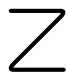
\includegraphics[keepaspectratio]{images/part002_15bf1a92.jpg}}

注. 注意两个等价的 (H) 函数可以有不等价的反函数，如两个函数 \(\log x\) 与 \(1 + \log x\) 的例子所示。

\setcounter{exercisegroup}{0}
\refstepcounter{exercisegroup}
\section*{第 \S\arabic{exercisegroup} 节习题}
\phantomsection
\addcontentsline{toc}{section}{第 \protect\S\arabic{exercisegroup} 节习题}

\begin{enumerate}
\def\labelenumi{\arabic{enumi})}
\tightlist
\item
  证明：对实变量 \(x\) （趋于 \(+\infty\) ），函数
\end{enumerate}

\[
f (x) = \left(x \cos^ {2} x + \sin^ {2} x\right) e ^ {x ^ {2}}
\]

单调，但它既不与 \(e^{x^2}\) 可比较，也不与 \(x^{1/2}e^{x^2}\) 弱可比较。

\begin{enumerate}
\def\labelenumi{\arabic{enumi})}
\setcounter{enumi}{1}
\tightlist
\item
  设 \(\varphi\) 是一个严格正的函数，对 \(x > 0\) 有定义且递增，并满足 \(\varphi \gg 1\) 。
\end{enumerate}

\begin{enumerate}
\def\labelenumi{\alph{enumi})}
\item
  证明：若函数 \(\log \varphi(x) / \log x\) 递增，则函数之间的关系 \(f \ll g\) （这些函数 \(>0\) ）蕴含 \(\varphi \circ f \ll \varphi \circ g\) （当 \(g \gg 1\) 时）。
\item
  给出一个例子，其中 \(\log \varphi(x)/\log x\) 递减，f 与 g 是两个 \textgreater0 的函数，满足 \(g \gg 1\) 且 \(f \sim g\) ，但 \(\varphi \circ f\) 不等价于 \(\varphi \circ g\) 。
\end{enumerate}

3) a) 设 \((\alpha_{i},\beta_{i})\) 是 \(n\) 个互异的实数对（由实数 \(\geqslant 0\) 组成），异于 \((0,0)\) ，且满足 \(\inf_{i}\alpha_{i} = \inf_{i}\beta_{i} = 0\) 。考察方程

\[
f (x, y) = \sum_ {i = 1} ^ {n} a _ {i} x ^ {\alpha_ {i}} y ^ {\beta_ {i}} \left(1 + \varphi_ {i} (x, y)\right) = 0
\]

其中诸 \(a_{i}\) 是 \(\neq0\) 的实数，诸 \(\varphi_{i}\) 是正方形 \(0\leqslant x\leqslant a,0\leqslant y\leqslant a\) 上的连续函数，且当 \((x,y)\) 趋于 \((0,0)\) 时趋于 0。假设存在一个函数 g，它在区间 {[}0,b{]} 上为正且连续，随 x 趋于 0，且满足 \(f(x,g(x))=0\) （对所有 \(x\in[0,b]\) ）。证明：对每个实数 \(\mu>0\) ，当 x 趋于 0 时 \(g(x)/x^{\mu}\) 趋于一个有限或无穷的极限（利用 V, p.~217, prop. 9，对每个数 \(t\geqslant0\) 考察方程 \(f(x,tx^{\mu})=0\) ）。

\begin{enumerate}
\def\labelenumi{\alph{enumi})}
\setcounter{enumi}{1}
\item
  为使 \(g(x)/x^{\mu}\) 趋于一个有限极限 \(\neq0\) ，必须 \(\mu\) 满足：至少存在两个互异的对 \((\alpha_{h},\beta_{h})\) 与 \((\alpha_{k},\beta_{k})\) ，使 \(\alpha_{h}+\mu\beta_{h}=\alpha_{k}+\mu\beta_{k}\) ，且对每个其余的对 \((\alpha_{i},\beta_{i})\) 有 \(\alpha_{i}+\mu\beta_{i}\geqslant\alpha_{h}+\mu\beta_{h}\) 。这样就得到有限多个可能的值 \(\mu_{j}(1\leqslant j\leqslant r)\) ；数 \(-1/\mu_{j}\) 是平面 \(R^{2}\) 中这样的仿射直线的斜率：这些直线至少包含点集 \((\alpha_{i},\beta_{i})\) 中的两个点，且该点集的其余各点都位于所考虑的直线上方（“牛顿多边形”）。
\item
  设 \(\mu_{1}\) 是诸数 \(\mu_{j}\) 中最小者。证明 \(g(x) / x^{\mu_1}\) 趋于一个有限极限（可能为零）。（首先证明总可假定：若 \(i\) 与 \(j\) 是两个互异的指标，则不能同时有 \(\alpha_{i} \leqslant \alpha_{j}\) 与 \(\beta_{i} \leqslant \beta_{j}\) ；由此推出可设 \(\alpha_{1} = 0\) ， \(\alpha_{i} > 0\) 与 \(\beta_{i} < \beta_{1}\) （对 \(i \neq 1\) ）；然后令 \(g(x) = t(x)x^{\mu_1}\) ，证明 \(t(x)\) 不能趋于 \(+\infty\) （当 \(x\) 趋于 0）。）
\end{enumerate}

\(d)\) 由 \(c\) ) 出发，对 \(r\) 作递归，推出存在一个指标 \(j\) ，使 \(g(x) / x^{\mu_j}\) 趋于一个有限极限 \(\neq 0\) （当 \(x\) 趋于 0）。

\setcounter{exercisegroup}{2}
\refstepcounter{exercisegroup}
\section*{第 \S\arabic{exercisegroup} 节习题}
\phantomsection
\addcontentsline{toc}{section}{第 \protect\S\arabic{exercisegroup} 节习题}

\begin{enumerate}
\def\labelenumi{\arabic{enumi})}
\item
  定义一个递增函数 \(g\) ，它在 \(+\infty\) 的某个邻域上有连续导数，使 \(g\) 与 \(1 / x\) 可比较到 1 阶，但 \(x\) 与 \(1 / g\) 不可比较到 1 阶（取 \(g'(x) = 1\) ，但在以点 \(x = n\) （ \(n\) 为整数 \(>0\) ）为中心的充分小区间上 \(g'\) 取非常大的值）。
\item
  设 f 与 g 是两个 \(\geqslant0\) 的函数（随 x 趋于 \(+\infty\) ），且可比较到 1 阶；若 h 是一个可导函数， \(\geqslant0\) 且递增（当 x 趋于 \(+\infty\) ），证明 hf 与 hg 可比较到 1 阶。
\item
  给出两个函数的例子：它们为正、递减、当 x 趋于 \(+\infty\) 时趋于 0、可比较到 1 阶，且使 \(xf(x)\) 与 \(xg(x)\) 不可比较到 1 阶（取 f 与 g 等价，且使
\end{enumerate}

\[
\frac {f ^ {\prime} (x)}{f (x)} + \frac {1}{x} \qquad \text { and } \qquad \frac {g ^ {\prime} (x)}{g (x)} + \frac {1}{x}
\]

不可比较）。

\begin{enumerate}
\def\labelenumi{\arabic{enumi})}
\setcounter{enumi}{3}
\tightlist
\item
  \begin{enumerate}
  \def\labelenumii{\alph{enumii})}
  \tightlist
  \item
    证明 \(\frac{\sin x}{\sqrt{x}} \sim \frac{\sin x}{\sqrt{x}} \left(1 + \frac{\sin x}{\sqrt{x}}\right)\) ，但积分 \(\int_{a}^{+\infty} \frac{\sin t}{\sqrt{t}} dt\) 收敛，而积分 \(\int_{a}^{+\infty} \frac{\sin t}{\sqrt{t}} \left(1 + \frac{\sin t}{\sqrt{t}}\right) dt\) 为无穷。
  \end{enumerate}
\end{enumerate}

\begin{enumerate}
\def\labelenumi{\alph{enumi})}
\setcounter{enumi}{1}
\item
  证明积分 \(\int_{a}^{+\infty}\frac{\sin t}{t}dt\) 与 \(\int_{a}^{+\infty}\frac{\sin^{2}t}{t^{2}}dt\) 都收敛，但 \(\int_{x}^{+\infty}\frac{\sin^{2}t}{t^{2}}dt\) 相对于 \(\int_{x}^{+\infty}\frac{\sin t}{t}dt\) 并非可忽略，尽管 \(\sin^{2}t/t^{2}\ll\sin t/t\) 。
\item
  考虑取值于 \(R^{2}\) 的两个连续函数（定义在 \([1, +\infty[\) 上）：
\end{enumerate}

\[
\mathbf {f}: x \mapsto \left(\frac {1}{x ^ {2}}, \frac {\sin x}{x}\right), \quad \mathbf {g}: x \mapsto \left(\frac {1}{x ^ {2}}, \frac {\sin x}{x} \left(1 + \frac {\sin x}{x}\right)\right).
\]

证明它们对 \(x\) 的任何值都不为零， \(\mathbf{f} \sim \mathbf{g}\) （当 \(x\) 趋于 \(+\infty\) 时），积分 \(\int_{a}^{+\infty} \mathbf{f}(t) dt\) 与 \(\int_{a}^{+\infty} \mathbf{g}(t) dt\) 收敛，但 \(\int_{x}^{+\infty} \mathbf{f}(t) dt\) 不等价于 \(\int_{x}^{+\infty} \mathbf{g}(t) dt\) （当 \(x\) 趋于 \(+\infty\) 时）。

5) 设 \(f\) 是定义在 \(+\infty\) 的某个邻域上的实凸函数，且满足 \(f(x) \gg x\) 。称 \(f\) 在 \(+\infty\) 的某个邻域上是正则凸的，如果对每个凸函数 \(g\) （定义在 \(+\infty\) 的某个邻域上）且满足 \(f \sim g\) ，也有 \(f_d' \sim g_r'\) 。

对每个数 \(\alpha > 0\) 与充分大的 x，设 \(k(\alpha, x)\) 是诸数 \(\left(f(y) - (y - x)f_{d}'(y)\right)/f(x)\) 的下确界（当 y 取遍 \(\geqslant x\) 且满足 \(f_{d}'(y) \leqslant (1 + \alpha)f_{d}'(x)\) 的数所成的集时）。类似地，设 \(h(\alpha, x)\) 是诸数

\[
\left(f (z) + (x - z) f _ {d} ^ {\prime} (z)\right) / f (x)
\]

（当 \(z\) 取遍 \(\leqslant x\) 且满足 \(f_d'(z) \geqslant (1 - \alpha)f_d'(x)\) 的数所成的集时）的下确界。设 \(\psi(\alpha) = \limsup_{x \to +\infty} k(\alpha, x)\) ， \(\varphi(\alpha) = \limsup_{x \to +\infty} h(\alpha, x)\) 。证明： \(f\) 在

\(+\infty\) 的某个邻域上正则凸的充分必要条件是，对一切充分小的 \(\alpha\) 有 \(\psi(\alpha) < 1\) 且 \(\varphi(\alpha) < 1\) 。

6) 设 \(\mathbf{f}\) 是某个区间 \([x_0, +\infty[\) （属于 \(\mathbf{R}\) ）上的连续向量函数，且对所有 \(\lambda \geqslant 0\) ，函数 \(\mathbf{f}(x + \lambda) - \mathbf{f}(x)\) 当 \(x\) 趋于 \(+\infty\) 时趋于 0。

\begin{enumerate}
\def\labelenumi{\alph{enumi})}
\tightlist
\item
  证明： \(\mathbf{f}(x+\lambda)-\mathbf{f}(x)\) 当 \(\lambda\) 属于任一紧区间 \(K=[a,b]\) （ \([0,+\infty[\) 中的）时随 1/x 一致地趋于 0。（用反证法：若存在一个序列 \((x_{n})\) 趋于 \(+\infty\) ，以及 K 中的点列 \((\lambda_{n})\) 使
\end{enumerate}

\[
\| \mathbf {f} (x _ {n} + \lambda_ {n}) - \mathbf {f} (x _ {n}) \| > \alpha > 0
\]

对每个 n 成立，则存在 \(J_{n}\) （ \(\lambda_{n}\) 在 K 中的一个邻域），使对每个 \(\lambda \in J_{n}\) 有 \(\|\mathbf{f}(x_{n} + \lambda) - \mathbf{f}(x_{n})\| > \alpha\) 。用归纳法构造一个递减的闭区间序列 \(I_{k} \subset K\) 与一个子序列 \((x_{n_{k}})\) （ \((x_{n})\) 的），使 \(\|\mathbf{f}(x_{n_{k}} + \lambda) - \mathbf{f}(x_{n_{k}})\| \geqslant \alpha/3\) 对每个 \(\lambda \in I_{k}\) 成立；为此注意，若 \(\delta_{k}\) 是 \(I_{k}\) 的长度而 q 是使 \(q\delta_{k} > b - a\) 的整数，则只要 x 充分大就有 \(\|\mathbf{f}(x + \delta_{k}) - \mathbf{f}(x)\| \leqslant \alpha/3q\) 。）

\begin{enumerate}
\def\labelenumi{\alph{enumi})}
\setcounter{enumi}{1}
\tightlist
\item
  由 \(a\) ) 推出 \(\int_{x}^{x + 1}\mathbf{f}(t)dt - \mathbf{f}(x)\) 当 \(x\) 趋于 \(+\infty\) 时趋于 0，并断定 \(\mathbf{f}(x) = o(x)\) 。
\end{enumerate}

\begin{enumerate}
\def\labelenumi{\arabic{enumi})}
\setcounter{enumi}{6}
\tightlist
\item
  设 g 是一个严格正的实函数，在某个区间 \([x_{0}, +\infty[\) 上连续，且对每个 \(\mu > 0\) 有 \(g(\mu x) \sim g(x)\) 。由习题 6 推出 g 相对于 x 的阶为 0。
\end{enumerate}

\setcounter{exercisegroup}{3}
\refstepcounter{exercisegroup}
\section*{第 \S\arabic{exercisegroup} 节习题}
\phantomsection
\addcontentsline{toc}{section}{第 \protect\S\arabic{exercisegroup} 节习题}

\begin{enumerate}
\def\labelenumi{\arabic{enumi})}
\item
  若通项为 \(u_{n} \geqslant 0\) 的级数收敛，则通项为 \(\sqrt{u_n u_{n+1}}\) 的级数也收敛。逆命题一般不成立；证明当级数 \((u_n)\) 递减时逆命题成立。
\item
  设 \((p_{n})\) 是一个递增的数 \textgreater{} 0 的序列（趋于 \(+\infty\) ）。
\end{enumerate}

\begin{enumerate}
\def\labelenumi{\alph{enumi})}
\tightlist
\item
  若比值 \(p_n / p_{n-1}\) 当 \(n\) 无限增大时趋于 1，证明
\end{enumerate}

\[
\sum_ {k = 1} ^ {n} \frac {p _ {k} - p _ {k - 1}}{p _ {k}} \sim \log p _ {n}
\]

\[
\sum_ {k = 1} ^ {n} p _ {k} ^ {\rho} (p _ {k} - p _ {k - 1}) \sim \frac {1}{\rho + 1} p _ {n} ^ {\rho + 1} \quad \text { for } \rho > - 1
\]

（应用 V, p.~237 的命题 2）。

\begin{enumerate}
\def\labelenumi{\alph{enumi})}
\setcounter{enumi}{1}
\item
  不对比值 \(p_{n}/p_{n-1}\) 作假设，证明通项为 \((p_{n}-p_{n-1})/p_{n}\) 的级数总有无穷和（区分 \(p_{n}/p_{n-1}\) 趋于 1 与不趋于 1 两种情形）。
\item
  证明对每个 \(\rho > 0\) ，通项为 \((p_n - p_{n-1}) / p_n p_{n-1}^\rho\) 的级数收敛（与通项为 \(\frac{1}{p_{n-1}^\rho} - \frac{1}{p_n^\rho}\) 的级数比较）。
\end{enumerate}

\begin{enumerate}
\def\labelenumi{\arabic{enumi})}
\setcounter{enumi}{2}
\item
  证明：对每个收敛级数 \((u_{n})\) （项 \(>0\) ），存在一个级数 \((v_{n})\) （具有无穷和、项 \(>0\) ），使 \(\liminf v_n / u_n = 0\) 。
\item
  设 \((u_{n})\) 是一个递减的数 \textgreater0 的序列；若存在一个整数 k，使从某个 n 起 \(ku_{kn} \geqslant u_{n}\) 对一切 n 成立，则通项为 \(u_{n}\) 的级数有无穷和。
\item
  设 \((u_{n})\) 是一个从某项起项 \(>0\) 的级数。证明：若
\end{enumerate}

\[
\operatorname * {l i m s u p} _ {n \to \infty} \left(\frac {u _ {n + 1}}{u _ {n}}\right) ^ {n} <   \frac {1}{e}
\]

则级数收敛；若 \(\liminf_{n\to\infty}\left(\frac{u_{n+1}}{u_n}\right)^n\geqslant\frac{1}{e}\) ，则级数有无穷和。

\begin{enumerate}
\def\labelenumi{\arabic{enumi})}
\setcounter{enumi}{5}
\item
  设 \((u_{n})\) 是由 \(\neq 0\) 的实数组成的级数，且 \(\lim_{n\to \infty}u_n = 0\) 。证明：若存在一个数 \(r\) 满足 \(0 < r < 1\) ，且从某个 n 起有 \(-1\leqslant u_{n + 1} / u_n\leqslant r\) ，则级数 \((u_{n})\) 收敛。
\item
  设 \((u_{n})\) 是一个项 \(>0\) 的收敛级数。
\end{enumerate}

\begin{enumerate}
\def\labelenumi{\alph{enumi})}
\tightlist
\item
  证明
\end{enumerate}

\[
\lim _ {n \rightarrow \infty} \frac {u _ {1} + 2 u _ {2} + \cdots + n u _ {n}}{n} = 0.
\]

\begin{enumerate}
\def\labelenumi{\alph{enumi})}
\setcounter{enumi}{1}
\tightlist
\item
  证明
\end{enumerate}

\[
\sum_ {n = 1} ^ {\infty} \frac {u _ {1} + 2 u _ {2} + \cdots + n u _ {n}}{n (n + 1)} = \sum_ {n = 1} ^ {\infty} u _ {n}
\]

\[
\left(\text { write } \frac {1}{n (n + 1)} = \frac {1}{n} - \frac {1}{n + 1}\right).
\]

\begin{enumerate}
\def\labelenumi{\alph{enumi})}
\setcounter{enumi}{2}
\tightlist
\item
  由 a) 与 b) 推出
\end{enumerate}

\[
\lim _ {n \to \infty} n (u _ {1} u _ {2} \dots u _ {n}) ^ {1 / n} = 0
\]

以及

\[
\sum_ {n = 1} ^ {\infty} \frac {(n ! u _ {1} u _ {2} \dots u _ {n}) ^ {1 / n}}{n + 1} <   \sum_ {n = 1} ^ {\infty} u _ {n}
\]

（应用 III, p.~93 的不等式 (8)）。

8) a) 设 \((z_{n})\) 是一个复数序列。证明：若通项分别为 \(z_{n}, z_{n}^{2}, \ldots, z_{n}^{q-1}, |z_{n}|^{q}\) 的级数都收敛，则通项因子为 \(1 + z_{n}\) 的无穷乘积收敛。

\begin{enumerate}
\def\labelenumi{\alph{enumi})}
\setcounter{enumi}{1}
\tightlist
\item
  若 \(z_{n}\) 是实数且通项为 \(z_{n}\) 的级数收敛，则通项因子为 \(1 + z_{n}\) 的无穷乘积在通项为 \(z_{n}^{2}\) 的级数收敛时收敛，且有
\end{enumerate}

\[
\underset {n = 1} {\overset {\infty} {\mathrm{P}}} (1 + z _ {n}) = 0 \quad \text { if } \quad \sum_ {n = 1} ^ {\infty} z _ {n} ^ {2} = + \infty .
\]

\begin{enumerate}
\def\labelenumi{\alph{enumi})}
\setcounter{enumi}{2}
\tightlist
\item
  对每个整数 \(p \geqslant 2\) 令
\end{enumerate}

\[
k _ {p} = [ \log \log p ], \quad h _ {p} = \sum_ {j = 1} ^ {p - 1} k _ {j}, \quad \omega_ {p} = \frac {2 \pi}{k _ {p}}.
\]

按下述方式定义复数序列 \((z_{n})\) ：对 \(n = h_{p} + m\) ， \(0 \leqslant m \leqslant k_{p} - 1\) ，令 \(z_{n} = e^{mi\omega_{p}} / \log p\) 。证明对每个整数 q \textgreater{} 0，通项为 \(z_{n}^{q}\) 的级数收敛，但通项因子为 \(1 + z_{n}\) 的乘积不收敛。

\begin{enumerate}
\def\labelenumi{\arabic{enumi})}
\setcounter{enumi}{8}
\tightlist
\item
  \begin{enumerate}
  \def\labelenumii{\alph{enumii})}
  \tightlist
  \item
    借助斯特林公式证明：函数 \(f_{n}(x) = \left|e^{-2x} - e^{-x}\sum_{k=0}^{n}(-1)^{k}\frac{x^{k}}{k!}\right|\) 在区间 \([0, +\infty[\) 上的最大值随 \(1/n\) 趋于 0。
  \end{enumerate}
\end{enumerate}

\begin{enumerate}
\def\labelenumi{\alph{enumi})}
\setcounter{enumi}{1}
\tightlist
\item
  由 a) 出发对整数 p 作归纳推出：对每个 \(\varepsilon > 0\) 存在一个多项式 \(g(x)\) ，使 \(\left|e^{-px} - e^{-x}g(x)\right| \leqslant \varepsilon\) 对每个 \(x \geqslant 0\) 成立（在 a) 中把 x 换成 px/2，并对 \(e^{-(p-1)x/2}\) 应用归纳假设）。
\end{enumerate}

\begin{enumerate}
\def\labelenumi{\arabic{enumi})}
\setcounter{enumi}{9}
\tightlist
\item
  对每个数 \(\alpha > 0\) 推出公式
\end{enumerate}

\[
1 ^ {\alpha n} + 2 ^ {\alpha n} + \dots + n ^ {\alpha n} \sim \frac {n ^ {\alpha n}}{1 - e ^ {- \alpha}}
\]

其中 n 趋于 \(+\infty\) 。

11) 对每个数 \(\alpha > 0\) 推出公式

\[
(1!) ^ {- \alpha / n} + (2!) ^ {- \alpha / n} + \dots + (n!) ^ {- \alpha / n} \sim \frac {1}{\alpha} \frac {n}{\log n}
\]

其中 \(n\) 趋于 \(+\infty\) （把每一项 \((p!)^{-\alpha / n}\) 与 \(n^{-\alpha p / n}\) 比较）。

\section*{附录习题}
\phantomsection
\addcontentsline{toc}{section}{附录习题}

\begin{enumerate}
\def\labelenumi{\arabic{enumi})}
\tightlist
\item
  设 \(\mathfrak{K}\) 是一个哈代域，使得对每个函数 \(f\in \mathfrak{K}\) （在 \(+\infty\) 的某个邻域上不恒为零）存在一个 \(\lambda >0\) 使
\end{enumerate}

\[
\frac {1}{e _ {m} (x ^ {\lambda})} \ll f (x) \ll e _ {m} (x ^ {\lambda})
\]

（m 是一个与 f 无关的整数）。

\begin{enumerate}
\def\labelenumi{\alph{enumi})}
\tightlist
\item
  设 \(u_{1}, u_{2}, \ldots, u_{p}\) 是 p 个形如 \(u_{k} = \log |z_{k}|\) 的函数，其中 \(z_{k} \in K\) 在 \(+\infty\) 的某个邻域上不为零。证明：对每个函数 g（在 \(+\infty\) 的某个邻域上不为零；属于哈代域 \(\mathfrak{K}(u_{1}, u_{2}, \ldots, u_{p})\) ，该域由把诸函数 \(u_{k}\) （ \(1 \leqslant k \leqslant p\) ）添加到 K 而得到），存在一个数 \(\mu > 0\) 使
\end{enumerate}

\[
\frac {1}{e _ {m} (x ^ {\mu})} \ll g (x) \ll e _ {m} (x ^ {\mu})
\]

（归结为 g 是系数在 K 中的 \(u_{k}\) 的多项式的情形，对 p 作归纳论证；然后对 p = 1，仿照 V, p.~248 引理 2 的做法对多项式 g 的次数作归纳论证）。

\begin{enumerate}
\def\labelenumi{\alph{enumi})}
\setcounter{enumi}{1}
\tightlist
\item
  设 \(u_{k}\) （ \(1 \leqslant k \leqslant p\) ）是 \(p\) 个形如 \(u_{k} = \exp(z_{k})\) 的函数，其中 \(z_{k} \in \mathcal{K}\) 。证明：对每个函数 \(g\) （属于哈代域 \(\mathcal{K}(u_{1}, u_{2}, \ldots, u_{p})\) ，在 \(+\infty\) 的某个邻域上不恒为零），存在一个数 \(\mu > 0\) 使
\end{enumerate}

\[
\frac {1}{e _ {m + 1} (x ^ {\mu})} \prec g (x) \prec e _ {m + 1} (x ^ {\mu})
\]

（类似的方法）。

\begin{enumerate}
\def\labelenumi{\alph{enumi})}
\setcounter{enumi}{2}
\tightlist
\item
  推出：若 \(f\) 是一个具有 \(n\) 项定义序列、且在 \(+\infty\) 的某个邻域上不恒为零的 (H) 函数，则存在一个数 \(\lambda > 0\) 使
\end{enumerate}

\[
\frac {1}{e _ {n} (x ^ {\lambda})} \ll f (x) \ll e _ {n} (x ^ {\lambda}).
\]

\begin{enumerate}
\def\labelenumi{\arabic{enumi})}
\setcounter{enumi}{1}
\tightlist
\item
  \begin{enumerate}
  \def\labelenumii{\alph{enumii})}
  \tightlist
  \item
    证明每个只有一项定义序列的 (H) 函数等价于形如 \(x^{p}(\log x)^{q}\) 或 \(x^{p}e^{g(x)}\) 之一的函数，其中 p 与 q 是有理整数，g 是 x 的多项式（习题 1 的方法）。
  \end{enumerate}
\end{enumerate}

\begin{enumerate}
\def\labelenumi{\alph{enumi})}
\setcounter{enumi}{1}
\tightlist
\item
  由 a) 推出：哈代域 \(\mathbf{R}(x,u_{1},\ldots,u_{p})\) （其中 \(u_{1},\ldots,u_{p}\) 是只有单项定义序列的 (H) 函数）中每个函数都等价于形如 \(x^{p}(\log x)^{q}e^{g(x)}\) 的函数，其中 p 与 q 是有理整数，g 是 x 的多项式。
\end{enumerate}

\begin{enumerate}
\def\labelenumi{\arabic{enumi})}
\setcounter{enumi}{2}
\item
  设 f 与 g 是两个 (H) 函数，使 f/g 相对于 \(l_{m}(x)\) 的阶为 0；证明：若 g 相对于 \(l_{m}(x)\) 的阶不为 0，则 \(f'/g' \sim f/g\) （比较 \(\log |f|\) 与 \(\log |g|\) ）。
\item
  设 \(\mathfrak{K}\) 是一个哈代域，使得对每个函数 \(f\in \mathfrak{K}\) （不等价于常数、且相对于 \(l_{m - 1}(x)\) 的阶为 0），存在一个常数 \(k\) 与一个有理整数 \(r\) ，使 \(f(x)\sim k(l_m(x))^r\) 。
\end{enumerate}

\begin{enumerate}
\def\labelenumi{\alph{enumi})}
\item
  设 z 是 K 中任一在 \(+\infty\) 的某个邻域上不恒为零的函数。证明：哈代域 \(\mathcal{K}(\log|z|)\) 中每个不等价于常数、且相对于 \(l_{m}(x)\) 的阶为 0 的函数 g，都等价于形如 \(k(l_{m+1}(x))^{r}\) 的函数（k 为常数，r 为有理整数）。（先考虑 g 是 \(\log|z|\) 的 p 次多项式、系数在 K 中的情形，并用习题 3 对 p 作归纳论证；若 g 是 \(\log|z|\) 的有理函数、系数在 K 中，则用习题 3 对分子的次数作归纳论证。）
\item
  证明 \(\mathfrak{K}(l_{m+1}(x))\) 中每个函数都等价于形如 \(f(x)(l_{m+1}(x))^r\) 的函数，其中 \(f \in \mathfrak{K}\) ， \(r\) 是有理整数。
\item
  设 z 是 K 中任一函数。证明：哈代域 \(\mathfrak{K}(e^{z})\) 中每个相对于 \(l_{m}(x)\) 的阶为 0 的函数 g 都等价于一个常数。（先考虑 \(g = u^{q} \mathrm{P}(u)\) 的情形，其中 \(u = e^{z}\) ，q 是有理整数， \(\mathrm{P}(u)\) 是 u 的 p 次多项式、系数在 K 中；然后用 a) 与习题 3 对 p 作归纳论证。再用习题 3 过渡到一般情形。）
\item
  把 a) 的结果推广到域 \(\mathfrak{K}(u_{1}, u_{2}, \ldots, u_{s})\) ，其中诸 \(u_{k}\) 形如 \(e^{z_{k}}\) 或 \(\log |z_{k}|\) ，诸 \(z_{k}\) 是 K 中在 \(+\infty\) 的某个邻域上不恒为零的函数（对 s 作归纳论证）。
\end{enumerate}

\begin{enumerate}
\def\labelenumi{\arabic{enumi})}
\setcounter{enumi}{4}
\tightlist
\item
  \begin{enumerate}
  \def\labelenumii{\alph{enumii})}
  \tightlist
  \item
    由习题 4 推出：若 f 是一个具有 n 项定义序列、不等价于常数、且相对于 \(l_{n-1}(x)\) 的阶为 0 的 (H) 函数，则存在一个常数 k 与一个有理整数 r，使 \(f(x) \sim k(l_n(x))^r\) 。
  \end{enumerate}
\end{enumerate}

\begin{enumerate}
\def\labelenumi{\alph{enumi})}
\setcounter{enumi}{1}
\tightlist
\item
  由习题 4 推出：若 \(f\) 是任一 (H) 函数，则存在一个整数 \(n\) ，使 \(n\) 阶对数判别法能够判定积分 \(\int_{a}^{+\infty} f(t) dt\) 收敛或为无穷。
\end{enumerate}

\begin{enumerate}
\def\labelenumi{\arabic{enumi})}
\setcounter{enumi}{5}
\tightlist
\item
  把函数 \(e_p\left((l_q(x))^{\mu}\right)\) 按整数 \(p\) 与 \(q\) 以及实数 \(\mu\) （设其 \(> 0\) 且 \(\neq 1\) ）的取值相互比较。
\end{enumerate}

7) 设 \(f\) 是一个具有 \(n\) 项定义序列的 (H) 函数。证明：若有 \(e_p((l_{q+1}(x))^{\beta}) \ll f(x) \ll e_p((l_q(x))^{\alpha})\) （相应地， \(e_p((l_q(x))^{\beta}) \ll f(x) \ll e_{p+1}((l_q(x))^{\alpha}))\) ），

则对每个 \(\beta > 0\) 与每个 \(\alpha\) （ \(0 < \alpha < 1\) ），必有 \(p + q + 1 < n\) （对 \(n\) 作归纳论证，使用与习题 1 (V, p.~263) 和 4 (V, p.~264) 类似的方法）。

\begin{enumerate}
\def\labelenumi{\arabic{enumi})}
\setcounter{enumi}{7}
\tightlist
\item
  \begin{enumerate}
  \def\labelenumii{\alph{enumii})}
  \tightlist
  \item
    设 \((f_{n})\) 是属于 \(\mathcal{H}(\mathfrak{F},\mathbf{R})\) 的递增连续函数序列，且对每个 n 有 \(f_{n} \ll f_{n+1}\) 。证明存在一个连续、递增、属于 \(\mathcal{H}(\mathfrak{F},\mathbf{R})\) 的函数 f，使对每个 n 有 \(f \gg f_{n}\) （归结为 \(f_{n} \leqslant f_{n+1}\) 的情形，并定义 f 使 \(f_{n}(x) \leqslant f(x) \leqslant f_{n+1}(x)\) （对 \(n \leqslant x \leqslant n+1\) ））。
  \end{enumerate}
\end{enumerate}

\begin{enumerate}
\def\labelenumi{\alph{enumi})}
\setcounter{enumi}{1}
\item
  设 \((f_n)\) 是属于 \(\mathcal{H}(\mathfrak{F},\mathbf{R})\) 的递增连续函数序列，且 \(1\ll f_{n + 1}\ll f_n\) 对每个 \(n\) 成立。证明存在一个函数 \(f\) ，连续、递增、属于 \(\mathcal{H}(\mathfrak{F},\mathbf{R})\) ，使 \(1\ll f\ll f_n\) 对每个 \(n\) 成立（归结为 \(f_{n + 1}\leqslant f_n\) 的情形，并证明可以定义一个递增的实数序列 \((x_{n})\) 与一个连续递增函数 \(f\) ，使 \(f_{n + 1}(x)\leqslant f(x)\leqslant f_n(x)\) （对 \(x_{n}\leqslant x\leqslant x_{n + 1}\) ））。
\item
  设 \((f_n), (g_n)\) 是两个属于 \(\mathcal{H}(\mathfrak{F}, \mathbf{R})\) 的连续递增函数序列，满足 \(f_n \ll f_{n+1}\) 、 \(g_m \gg g_{m+1}\) 且 \(f_n \ll g_m\) （对所有 \(m\) 与 \(n\) ）；证明存在一个函数 \(h\) ，连续、递增、属于 \(\mathcal{H}(\mathfrak{F}, \mathbf{R})\) ，使 \(f_n \ll h \ll g_m\) （对所有 \(m\) 与 \(n\) ）（类似的方法）。
\end{enumerate}

特别地，证明存在一个连续递减函数 \(f\) （属于 \(\mathcal{H}(\mathfrak{F},\mathbf{R})\) ），使任何对数判别法都不能判定积分 \(\int_{a}^{+\infty}f(t)dt\) 收敛或为无穷（“杜·布瓦–雷蒙定理”）。

\begin{enumerate}
\def\labelenumi{\arabic{enumi})}
\setcounter{enumi}{8}
\item
  证明级数 \(\sum_{n=1}^{\infty} \frac{e_n(x)}{e_n(n)}\) 在 \(\mathbf{R}\) 的每个紧子集上一致收敛，且其和 \(f(x)\) 满足： \(f(x) \gg e_n(x)\) 对每个整数 \(n\) 成立。
\item
  证明存在一个递增函数 \(f\) ，它有定义、连续且 \(> 0\) （对 \(x \geqslant 0\) ），使 \(f(2x) = 2^{f(x)}\) 对所有 \(x \geqslant 0\) 成立；由此推出 \(f(x) \gg e_n(x)\) 对每个整数 \(n\) 成立。
\item
  设 \(f\) 是一个递增函数，连续且 \(\geqslant 0\) （对 \(x \geqslant 0\) 有定义），且 \(f(x) \gg e_n(x)\) 对每个整数 \(n\) 成立；证明：若 \(g\) 是 \(f\) 的反函数，则 \(1 \ll g(x) \ll l_n(x)\) 对每个整数 \(n\) 成立。
\end{enumerate}

12) 对每个整数 \(n > 0\) ，设 \(n = \sum_{k=0}^{\infty} \varepsilon_k 2^k\) 是 \(n\) 的二进展开（ \(\varepsilon_k\) 是整数，除有限个指标外均为零， \(0 \leqslant \varepsilon_k \leqslant 1\) ）。令

\[
\alpha (n) = \sum_ {k = 0} ^ {\infty} \varepsilon_ {k}, \quad \mathrm{A} _ {1} (n) = \sum_ {j = 1} ^ {n} \alpha (j), \quad \mathrm{A} _ {2} (n) = \sum_ {j = 1} ^ {n} \alpha (\alpha (j)).
\]

\begin{enumerate}
\def\labelenumi{\alph{enumi})}
\tightlist
\item
  证明公式 \(\mathrm{A}_1(n) = \sum_{k=0}^{\infty}(k+2)\varepsilon_k 2^{k-1}\) 。由此推出公式
\end{enumerate}

\[
\mathrm{A} _ {1} (n) = \frac {n}{2} \frac {\log n}{\log 2} + o (n \log \log n)
\]

其中 \(n\) 无限增大（把表示 \(\mathrm{A}_1(n)\) 的和分解成两部分：第一个和中指标 \(k\) 从 0 变到 \(\mu(n)\) ，第二个和中从 \(\mu(n)\) 变到 \(n_1\) ，这里 \(n_1\) 是数 \(k\) （使 \(\varepsilon_k \neq 0\) ）中最大者，而 \(\mu(n)\) 取得适当；用 V, p.~239 的命题 6 估计第一个和的上界，然后估计第二个和与 \(n_1n / 2\) 之差。

\begin{enumerate}
\def\labelenumi{\alph{enumi})}
\setcounter{enumi}{1}
\tightlist
\item
  建立关系式
\end{enumerate}

\[
\sum_ {j = 0} ^ {2 ^ {m} - 1} f (\alpha (j)) = \sum_ {k = 0} ^ {m} \binom {m} {k} f (k)
\]

其中 \(f\) 是定义在 \(\mathbf{N}\) 上的任意函数（对给定的 \(k\) ，考察 \(j < 2^{m}\) 中使 \(\alpha(j) = k\) 的个数）。

\begin{enumerate}
\def\labelenumi{\alph{enumi})}
\setcounter{enumi}{2}
\tightlist
\item
  对 \(m = 2^r - 1\) ，证明 \(\alpha(m - j) + \alpha(j) = r\) 。由此并借助 \(b\) ) 推出
\end{enumerate}

\[
\mathrm{A} _ {2} (2 ^ {m}) = r 2 ^ {m - 1} \sim \frac {2 ^ {m} \log \log 2 ^ {m}}{2 \log 2}.
\]

\begin{enumerate}
\def\labelenumi{\alph{enumi})}
\setcounter{enumi}{3}
\tightlist
\item
  对 \(m = 2^{r}\) ，证明
\end{enumerate}

\[
\mathrm{A} _ {2} (2 ^ {m}) = 2 \mathrm{A} _ {2} (2 ^ {m - 1}) + 2 ^ {m - 1} - \sum_ {j = 0} ^ {m - 1} \binom {m - 1} {j} \Delta (j + 1)
\]

其中我们令 \(\alpha(n+1)-\alpha(n)=1-\Delta(n+1)\) （对所有 \(n\) ；利用 \(b\) ）以及关系式 \(\alpha(2^{k}+r)=\alpha(r)+1\) （对 \(r<2^{k}\) ））。证明 \(\sum_{j=0}^{m-1}\binom{m-1}{j}\Delta(j+1)\leqslant r^{m-2}\) （注意 \(\Delta(j+1)=0\) （若 \(j\) 为偶数），且 \(\Delta(j+1)\leqslant\log j/\log 2\) 对所有 \(j\) 成立）。借助 \(c\) ) 推出

\[
\mathrm{A} _ {2} (2 ^ {m}) \geqslant \frac {3}{2} r 2 ^ {m - 1} \geqslant \frac {3}{2} \frac {2 ^ {m} \log \log 2 ^ {m}}{2 \log 2}.
\]

由 \(c\) ) 与这个关系式断定： \(\mathrm{A}_2(n)\) 当 \(n\) 趋于 \(+\infty\) 时不等价于任何 (H) 函数。

\begin{enumerate}
\def\labelenumi{\arabic{enumi})}
\setcounter{enumi}{12}
\tightlist
\item
  设 \(f\) 是一个满足 \(1 \prec f(x) \prec x\) 的 (H) 函数。证明在泰勒公式
\end{enumerate}

\[
\begin{array}{l} f (x + f (x)) = f (x) + f (x) f ^ {\prime} (x) + \frac {1}{2 !} (f (x)) ^ {2} f ^ {\prime \prime} (x) + \dots + \\ \qquad + \frac {1}{n !} (f (x)) ^ {n} f ^ {(n)} (x) + \frac {1}{(n + 1) !} (f (x)) ^ {n + 1} f ^ {(n + 1)} (x + \theta f (x)) \end{array}
\]

（ \(0 < \theta < 1\) ，I, p.~42, exerc. 9）中，每一项相对于前一项都可忽略。若 f 相对于 x 的阶 \textless{} 1，则只要 n 充分大，这个和中的最后一项随 1/x 趋于 0。

\begin{enumerate}
\def\labelenumi{\arabic{enumi})}
\setcounter{enumi}{13}
\tightlist
\item
  由习题 13 推出：若 \(f\) 是一个使 \(\log f(e^x)\) 的阶 \(< 1\) （相对于 \(x\) ）的 (H) 函数，则函数 \(f(xf(x))\) 等价于形如 \(e^{g(x)}\) 的函数，其中 \(g\) 是 \(x\) 、 \(\log f(x)\) 以及后一函数的若干导数的有理函数。
\end{enumerate}

15) 设 \(f\) 是一个 (H) 函数，在 \(+\infty\) 的某个邻域上凸，且满足 \(f(x) \gg x\) 。对每个 \(\alpha > 0\) ，设 \(x_{\alpha}\) 是使 \(f'(x_{\alpha}) = (1 + \alpha)f'(x)\) 的点。

\begin{enumerate}
\def\labelenumi{\alph{enumi})}
\tightlist
\item
  若 \(f\) 的阶为 \(+\infty\) （相对于 \(x\) ），证明
\end{enumerate}

\[
x _ {\alpha} - x \sim \log (1 + \alpha) \frac {f (x)}{f ^ {\prime} (x)}
\]

（利用命题 2 (V, p.~251) 与 4 (V, p.~255)，把泰勒公式应用于 \(\log f'(x)\) ）。证明 \(\left(f(x_{\alpha}) - (x_{\alpha} - x)f'(x_{\alpha})\right)/f(x)\) 趋于 \((1 + \alpha)\left(1 - \log(1 + \alpha)\right)\) （当 \(x\) 趋于 \(+\infty\) 时）。

\begin{enumerate}
\def\labelenumi{\alph{enumi})}
\setcounter{enumi}{1}
\tightlist
\item
  若 \(f\) 的阶为 \(r > 1\) （相对于 \(x\) ），证明
\end{enumerate}

\[
x _ {\alpha} \sim (1 + \alpha) ^ {1 / (r - 1)} x
\]

（注意由 V, p.~255 的命题 4，若 \(f_{1}\) 的阶为 0（相对于 \(x\) ），则 \(f_{1}(kx) \sim f_{1}(x)\) 对每个常数 \(k\) 成立）。推出 \(\left(f(x_{\alpha}) - (x_{\alpha} - x)f'(x_{\alpha})\right) / f(x)\) 趋于

\[
r (1 + \alpha) - (r - 1) (1 + \alpha) ^ {r / (r - 1)}
\]

（当 \(x\) 趋于 \(+\infty\) 时）。

\begin{enumerate}
\def\labelenumi{\alph{enumi})}
\setcounter{enumi}{2}
\tightlist
\item
  最后设 \(f\) 相对于 \(x\) 的阶为 1。令 \(f(x) = xf_1(x)\) ，证明
\end{enumerate}

\[
x _ {\alpha} - x \sim \log (1 + \alpha) \frac {f _ {1} (x)}{f _ {1} ^ {\prime} (x)}
\]

（考察 \(f_{1}\) 的反函数，其阶为 \(+\infty\) （相对于 \(x\) ））。推出 \(\left(f(x_{\alpha}) - (x_{\alpha} - x)f'(x_{\alpha})\right) / f(x)\) 趋于 \(-\infty\) （当 \(x\) 趋于 \(+\infty\) 时）。

类似地，设 \(x_{\alpha}'\) 是使 \(f'(x_{\alpha}') = (1 - \alpha)f'(x)\) 的点（ \(0 < \alpha < 1\) ）。叙述与前面类似的表达 \(x - x_{\alpha}'\) 的主部以及

\[
\left(f (x _ {\alpha} ^ {\prime}) + (x - x _ {\alpha} ^ {\prime}) f ^ {\prime} (x _ {\alpha} ^ {\prime})\right) / f (x)
\]

（当 \(x\) 趋于 \(+\infty\) 时）的极限的公式。

由这些结果断定： \(f\) 是 \(+\infty\) 的某个邻域上的正则凸函数 (V, p.~260, exerc. 5)。

\makeatletter
\gdef\@chapapp{\chaptername}
\makeatother
\renewcommand{\thechapter}{\chinese{chapter}}
\renewcommand{\thesection}{\S\arabic{section}}
\setcounter{chapter}{5}
\chapter{广义泰勒展开：欧拉–麦克劳林求和公式}

\section{广义泰勒展开}

\subsection{多项式代数上的复合算子}

设 K 为特征 0 的交换域，K{[}X{]} 为 K 上一个未定元的多项式代数（Alg., IV. 1）；在本节中，我们把 K{[}X{]} 上的算子理解为向量空间 K{[}X{]} （在 K 上）到其自身的线性映射 U；由于单项式 \(X^{n}\) （ \(n \geqslant 0\) ）构成此空间的一组基，U 由多项式 \(U(X^{n})\) 确定；确切地说，若 \(f(X) = \sum_{k=0}^{\infty} \lambda_{k} X^{k}\) ，其中 \(\lambda_{k} \in K\) ，则 \(U(f) = \sum_{k=0}^{\infty} \lambda_{k} U(X^{k})\) 。

若 \(\mathbf{G}\) 是 \(\mathbf{K}\) 上的一个含单位元的交换代数，则 \(\mathbf{G}\) -模 \(\mathrm{G}[\mathrm{X}]\) 是由把 \(\mathbf{K}\) -向量空间 \(\mathrm{K}[\mathrm{X}]\) 的标量域扩张到 \(\mathrm{G}\) 而得到的；每个算子 \(U\) （定义在 \(\mathrm{K}[\mathrm{X}]\) 上）都以唯一的方式扩张为 \(\mathrm{G}\) -模 \(\mathrm{G}[\mathrm{X}]\) 到其自身的一个线性映射，我们仍将它记作 \(U\) （Alg., II, p.~278）；对每个元素 \(g(\mathrm{X}) = \sum_{k=0}^{\infty} \gamma_k X^k\) ，其中 \(\gamma_k \in \mathrm{G}\) ，有 \(U(g) = \sum_{k=0}^{\infty} \gamma_k U(X^k)\) 。

特别地，考虑 \(\mathrm{G} = \mathrm{K}[\mathrm{Y}]\) 的情形；这时 \(\mathrm{G}[\mathrm{X}]\) 是环 \(\mathrm{K}[\mathrm{X},\mathrm{Y}]\) ，即 \(\mathrm{K}\) 上两个未定元的多项式环；为避免混淆，我们把 \(U\) 到 \(\mathrm{G}[\mathrm{X}]\) 上的扩张记作 \(U_{\mathrm{X}}\) 。于是，对任意多项式 \(g(\mathrm{X},\mathrm{Y}) = \sum_{k=0}^{\infty}\gamma_k(\mathrm{Y})\mathrm{X}^k\) （其中 \(\gamma_k(Y)\in \mathrm{K}[\mathrm{Y}]\) ）有 \(U_{\mathrm{X}}(g) = \sum_{k=0}^{\infty}\gamma_k(\mathrm{Y})U(\mathrm{X}^k)\) 。由于 \(U_{\mathrm{X}}\) 是线性的，可以看出，若把它写成 \(g(\mathrm{X},\mathrm{Y}) = \sum_{h=0}^{\infty}\beta_h(\mathrm{X})\mathrm{Y}^h\) ，则也有 \(U_{\mathrm{X}}(g) = \sum_{h=0}^{\infty}U(\beta_h)\mathrm{Y}^h\) 。

在把 X 对应到 Y 的 K{[}X{]} 到 K{[}Y{]} 上的典范同构下，算子 U 变换为 K{[}Y{]} 上的一个算子；为避免混淆，我们把它记作 \(U_{Y}\) ，于是 \(U_{\mathrm{Y}}(f(\mathrm{Y}))\) 就是在多项式 \(U(f(\mathrm{X})) = U_{\mathrm{X}}(f(\mathrm{X}))\) 中把 X 换成 Y 所得到的多项式。这个算子 \(U_{Y}\) 又可以扩张为一个算子（仍记作 \(U_{Y}\) ），它定义在 K{[}X,Y{]} 上：若 \(g(\mathrm{X}, \mathrm{Y}) = \sum_{h=0}^{\infty} \beta_{h}(\mathrm{X}) \mathrm{Y}^{h}\) ，则 \(U_{\mathrm{Y}}(g(\mathrm{X}, \mathrm{Y})) = \sum_{h=0}^{\infty} \beta_{h}(\mathrm{X}) U_{\mathrm{Y}}(\mathrm{Y}^{h})\) 。

作为这些扩张的一个例子，我们举出 K{[}X{]} 上的求导算子 D （Alg., IV. 6），它给出偏求导算子 \(D_{X}\) 与 \(D_{Y}\) （定义在 K{[}X,Y{]} 上）。

对每个多项式 \(f \in K[X]\) ，我们用 \(T_{Y}(f)\) 表示多项式 \(f(X + Y)\) （它属于 K{[}X,Y{]}）；映射 \(T_{Y}\) 是从 K{[}X{]} 到 K{[}X,Y{]} 中的一个 K-线性映射，称为平移算子。

定义 1. 称 K{[}X{]} 上的算子 U 为复合算子，如果它与平移算子可交换，也就是说，如果 \(U_{X}T_{Y} = T_{Y}U\) 。

换句话说，若 \(f\) 是 \(\mathbf{K}[\mathbf{X}]\) 中的任意一个多项式，且 \(g = U(f)\) ，则必须有 \(g(\mathbf{X} + \mathbf{Y}) = U_{\mathbf{X}}(f(\mathbf{X} + \mathbf{Y}))\) 。

由这个定义立即得出，对每个多项式 \(f(\mathrm{X}) \in \mathrm{K}[\mathrm{X}]\) ，按上述记号有

\[
U _ {\mathrm{X}} \big (f (\mathrm{X} + \mathrm{Y}) \big) = U _ {\mathrm{Y}} \big (f (\mathrm{X} + \mathrm{Y}) \big).\tag{1}
\]

例. 1) 对每个 \(\lambda \in \mathbf{K}\) ，把每个多项式 \(f(\mathbf{X})\) 对应到多项式 \(f(\mathbf{X} + \lambda)\) 的算子是一个复合算子。

\begin{enumerate}
\def\labelenumi{\arabic{enumi})}
\setcounter{enumi}{1}
\tightlist
\item
  K{[}X{]} 上的求导 D 是一个复合算子（参见命题 1）。
\end{enumerate}

注. 由于 K 是无限域，K{[}X{]} 上的算子 U 是复合算子，当且仅当对每个多项式 \(f \in K[X]\) 和每个元素 \(\alpha \in K\) ，令 \(g = U(f)\) ，有 \(g(X + \alpha) = U(f(X + \alpha))\) 。（Alg., IV. 16, cor.）

显然，复合算子的以 K 为系数的每个线性组合仍是复合算子；两个复合算子的复合（乘积）也是如此。换句话说，复合算子构成一个子代数 \(\Gamma\) ，含于向量空间 K{[}X{]} 的自同态代数中。

命题 1. K{[}X{]} 上的算子 U 是复合算子的充分必要条件为：它与 K{[}X{]} 上的求导 D 可交换。

事实上，泰勒公式表明，对每个多项式 \(f \in K[X]\) 有

\[
U _ {\mathrm{X}} \big (f (\mathrm{X} + \mathrm{Y}) \big) = U _ {\mathrm{X}} \left(\sum_ {k = 0} ^ {\infty} \frac {1}{k !} \mathrm{Y} ^ {k} \mathrm{D} ^ {k} f (\mathrm{X})\right) = \sum_ {k = 0} ^ {\infty} \frac {1}{k !} \mathrm{Y} ^ {k} U \big (\mathrm{D} ^ {k} f (\mathrm{X}) \big);
\]

若令 \(g = U(f)\) ，则有

\[
g (\mathrm{X} + \mathrm{Y}) = \sum_ {k = 0} ^ {\infty} \frac {1}{k !} \mathrm{Y} ^ {k} \mathrm{D} ^ {k} g (\mathrm{X}) = \sum_ {k = 0} ^ {\infty} \frac {1}{k !} \mathrm{Y} ^ {k} \mathrm{D} ^ {k} (U (f (\mathrm{X})))
\]

于是，为使 U 是复合算子，必须有 \(UD^{k} = D^{k}U\) （对每个整数 \(k \geqslant 1\) ），特别地有 \(UD = DU\) 。反之，若这一关系成立，则由对 k 的归纳法，它蕴含 \(UD^{k} = D^{k}U\) （对每个整数 \(k \geqslant 1\) ）；于是泰勒公式表明 \(g(X + Y) = U_{X}(f(X + Y))\) 。

对每个多项式 \(f \in K[X, Y]\) ，我们用 \(U_{0}(f)\) 表示多项式 \(U_{X}(f)\) 中不含 X 的项；特别地，若 \(f \in K[X]\) ，则 \(U_{0}(f)\) 是 \(U(f)\) 中的常数项，而 \(U_{0}\) 是 K{[}X{]} 上的一个线性型。对每个多项式 \(f \in K[X]\) ，令 \(g = U(f)\) ；由 VI, p.~270 的定义 1

\[
g (\mathrm{X} + \mathrm{Y}) = U _ {\mathrm{X}} (f (\mathrm{X} + \mathrm{Y})) = U _ {\mathrm{X}} \left(\sum_ {k = 0} ^ {\infty} \frac {1}{k !} \mathrm{X} ^ {k} \mathrm{D} ^ {k} f (\mathrm{Y})\right) = \sum_ {k = 0} ^ {\infty} \frac {1}{k !} U (\mathrm{X} ^ {k}) \mathrm{D} ^ {k} f (\mathrm{Y})
\]

而若在这个公式中把 X 换成 0 ，就得到

\[
g (\mathrm{Y}) = \sum_ {k = 0} ^ {\infty} \frac {1}{k !} U _ {0} (\mathrm{X} ^ {k}) \mathrm{D} ^ {k} f (\mathrm{Y}).
\]

于是可以看出

\[
U (f (\mathrm{X})) = \sum_ {k = 0} ^ {\infty} \frac {1}{k !} \mu_ {k} \mathrm{D} ^ {k} f (\mathrm{X})\tag{2}
\]

其中 \(\mu_{k}\) 是多项式 \(U(\mathbf{X}^k)\) 的常数项。

这个公式表明，诸 \(\mu_{k}\) 完全确定了复合算子 U；反过来，若 \((\mu_{n})\) 是 K 中元素的一个任意序列，则公式 (2) 定义了一个算子 U，它显然与 D 可交换，因而（VI, p.~270, prop. 1）是一个复合算子。今后我们把 (2) 写成如下形式

\[
U = \sum_ {k = 0} ^ {\infty} \frac {1}{k !} \mu_ {k} D ^ {k}.\tag{3}
\]

这个公式可以用拓扑语言解释如下：若在 K{[}X{]} 上考虑离散拓扑，并在自同态代数 \(\operatorname{End}(\operatorname{K}[X])\) （由 K{[}X{]} 的自同态组成）上考虑单收敛拓扑（Gen.~Top., X, p.~277），则以 \(\frac{1}{k!}\mu_{k}D^{k}\) 为通项的级数在 \(\operatorname{End}(\operatorname{K}[X])\) 中交换收敛，且其和为 U （Gen.~Top., III, p.~269）。

公式 (3) 表明，对形式级数 \(u(S) = \sum_{k=0}^{\infty} \alpha_k S^k\) （\(K\) 上一个未定元的，Alg., IV. 41），可以对应一个复合算子 \(U = \sum_{k=0}^{\infty} \alpha_k D^k\) ，今后我们把它记作 \(u(D)\) 。这一注记可以按如下方式加以阐明：

定理 1. 把每个形式级数 \(u(\mathbf{S}) = \sum_{k=0}^{\infty} \alpha_k \mathbf{S}^k\) （\(\mathbf{K}\) 上一个未定元的）对应到复合算子 \(u(\mathbf{D}) = \sum_{k=0}^{\infty} \alpha_k \mathbf{D}^k\) （\(\mathrm{K}[\mathrm{X}]\) 上的）的映射，是形式级数代数 \(\mathrm{K}[[\mathrm{S}]]\) 到复合算子代数 \(\Gamma\) 上的一个同构。

立即可以验证这个映射是一个同态。剩下要证的是它是单射，换句话说，关系 \(\sum_{k=0}^{\infty}\alpha_{k}D^{k}=0\) 蕴含对每个 k 都有 \(\alpha_{k}=0\) ；而 \(h!\alpha_{h}\) 是把 \(\sum_{k=0}^{\infty}\alpha_{k}D^{k}\) 作用于 \(X^{h}\) 所得多项式的常数项，由此即得定理。

推论. 复合算子代数 \(\Gamma\) （K{[}X{]} 中的）是交换的。

例. 若 \(U\) 是把每个多项式 \(f(\mathrm{X})\) 对应到 \(f(\mathrm{X} + \lambda)\) （其中 \(\lambda \in \mathbf{K}\) ）的算子，则有 \(U_0(\mathrm{X}^k) = \lambda^k\) ，从而 \(U = \sum_{k=0}^{\infty} \frac{1}{k!} (\lambda \mathrm{D})^k\) 。与 \(e^x\) 的级数展开（III, p.~105）相类比，我们用 \(e^{\mathrm{S}}\) 或 \(\exp(\mathrm{S})\) 表示形式级数 \(\sum_{n=0}^{\infty} \frac{1}{n!} \mathrm{S}^n\) （环 \(\mathrm{K}[[\mathrm{S}]]\) 中的）；于是可以写 \(U = e^{\lambda \mathrm{D}}\) 。在这论证中把域 \(\mathrm{K}\) 换成有理分式域 \(\mathrm{K}(\mathrm{Y})\) ，同样可以看出平移算子 \(T_{\mathrm{Y}}\) 可写成 \(e^{\mathrm{YD}}\) 。

此外，在 K 上两个未定元的形式级数环 K{[}{[}S, T{]}{]} 中有

\[
\begin{array}{l} (\exp S) (\exp T) = \sum_ {p, q} \frac {S ^ {p}}{p !} \frac {T ^ {q}}{q !} \\ = \sum_ {n = 0} ^ {\infty} \frac {1}{n !} \left(\binom {n} {0} S ^ {n} + \binom {n} {1} S ^ {n - 1} T + \dots + \binom {n} {n} T ^ {n}\right) \\ = \exp (S + T) \end{array}\tag{4}
\]

特别地，有

\[
(\exp S) (\exp (- S)) = 1\tag{5}
\]

这就说明我们引入的记号是合理的。

按语. 形式级数代数 K{[}{[}S{]}{]} 与复合算子代数 \(\Gamma\) （K{[}X{]} 上的）之间的同构，有时使我们能用对相应的复合算子证明命题的办法，最简单地证明关于形式级数的命题（参见 VI, p.~274, prop. 6）。

\subsection{与复合算子相联系的阿佩尔多项式}

给定一个复合算子 \(U = \sum_{k=0}^{\infty} \alpha_k \mathrm{D}^k \neq 0\) ，设 \(p\) 为整数 \(k\) （使 \(\alpha_k \neq 0\) 的）中最小的一个；我们称 \(p\) 为算子 \(U\) 的阶。

命题 2. 每个 0 阶复合算子在复合算子代数 \(\Gamma\) （K{[}X{]} 上的）中可逆。

事实上，形式级数 \(\sum_{k=0}^{\infty}\alpha_{k}S^{k}\) （满足 \(\alpha_{0}\neq0\) ）在环 K{[}{[}S{]}{]} 中可逆（Alg., IV. 41）；于是命题由 VI, p.~271 的定理 1 得出。

命题 3. 设 U 是一个 p 阶复合算子；则 \(U(f) = 0\) （对每个次数 \textless{} p 的多项式 f）；对每个多项式 \(f \neq 0\) （次数 \(n \geqslant p\) 的），\(U(f)\) 是一个次数为 n - p 的多项式 \(\neq 0\) 。

这是 VI, p.~271 的公式 (2) 与 \(U\) 的阶的定义的直接推论。

显然，每个算子 \(U\) （\(p\) 阶的）都可以以唯一的方式写成 \(U = \mathrm{D}^p V = V\mathrm{D}^p\) ，其中 \(V\) 是一个 0 阶算子（从而可逆）。

定义 2. 设 \(U = \mathrm{D}^p V\) 是一个 \(p\) 阶复合算子（\(\mathrm{K}[\mathrm{X}]\) 上的）。多项式 \(u_n(\mathrm{X}) = V^{-1}(\mathrm{X}^n)\) 称为指标为 \(n\) 而与算子 \(U\) 相联系的阿佩尔多项式。

\[
\text {   If   } V ^ {- 1} = \sum_ {k = 0} ^ {\infty} \frac {1}{k !} \beta_ {k} D ^ {k} (\text {   with   } \beta_ {0} \neq 0) \text {   one   thus   has   }
\]

\[
u _ {n} (\mathrm{X}) = \sum_ {k = 0} ^ {n} {\binom {n} {k}} \beta_ {k}   \mathrm{X} ^ {n - k}.\tag{6}
\]

可以验证 \(u_{n}\) 是一个 \(n\) 次多项式（prop. 3）；此外

\[
u _ {n} (0) = \beta_ {n}.
\]

命题 4. 与 \(U\) 相联系的阿佩尔多项式满足下列关系

\[
\frac {d u _ {n}}{d \mathrm{X}} = n u _ {n - 1}\tag{7}
\]

\[
u _ {n} (\mathrm{X} + \mathrm{Y}) = \sum_ {k = 0} ^ {n} {\binom {n} {k}} u _ {n - k} (\mathrm{X})   \mathrm{Y} ^ {k}\tag{8}
\]

\[
U \left(u _ {n} (\mathrm{X})\right) = \frac {n !}{(n - p) !} \mathrm{X} ^ {n - p}.\tag{9}
\]

这些公式事实上分别等价于下列关系（记住定义 2）：

\[
\mathbf {D} V ^ {- 1} = V ^ {- 1} \mathbf {D}\tag{10}
\]

\[
\left(\exp \left(\mathrm{YD} _ {\mathrm{X}}\right)\right) V _ {\mathrm{X}} ^ {- 1} = V _ {\mathrm{X}} ^ {- 1} \exp \left(\mathrm{YD} _ {\mathrm{X}}\right)\tag{11}
\]

\[
U V ^ {- 1} = \mathbf {D} ^ {p}.\tag{12}
\]

命题 5. 对每个多项式 \(f \in \mathrm{K}[\mathrm{X}]\) 和每个复合算子 \(U\) （\(p\) 阶的），有

\[
f ^ {(p)} (\mathrm{X} + \mathrm{Y}) = \sum_ {k = 0} ^ {\infty} \frac {1}{k !} U (f ^ {(k)} (\mathrm{X})) u _ {k} (\mathrm{Y})\tag{13}
\]

（广义泰勒展开）。

事实上，若令 \(U = \mathrm{D}^p V = V\mathrm{D}^p\) ，则有（VI, p.~270, 公式 (1)）

\[
V _ {\mathrm{X}} ^ {- 1} (f (\mathrm{X} + \mathrm{Y})) = V _ {\mathrm{Y}} ^ {- 1} (f (\mathrm{X} + \mathrm{Y})) = \sum_ {k = 0} ^ {\infty} \frac {1}{k !} f ^ {(k)} (\mathrm{X}) u _ {k} (\mathrm{Y})\tag{14}
\]

这是由泰勒公式及 VI, p.~273 的定义 2 得到的；只需对公式 (14) 的首末两项应用算子 \(U_{\mathrm{X}}\) 即得 (13)。

\subsection{阿佩尔多项式的生成级数}

设 E 为一个未定元 S 的形式级数环，其系数取在多项式环 K{[}X{]} 中（Alg., IV. 41）；换句话说，即形式级数 \(g(\mathrm{X}, \mathrm{S}) = \sum_{n=0}^{\infty} \alpha_n(\mathrm{X}) \mathrm{S}^n\) 组成的环，其中诸 \(\alpha_n\) 属于 K{[}X{]}。对每个算子 \(U\) （K{[}X{]} 上的），定义 E 到其自身的一个映射 \(U_{\mathrm{X}}\) 如下：置 \(U_{\mathrm{X}}(g(\mathrm{X}, \mathrm{S})) = \sum_{n=0}^{\infty} U(\alpha_n)\mathrm{S}^n\) 。显然，E 是以 K 为系数的未定元 S 的形式级数环 K{[}{[}S{]}{]} 上的一个模；由 \(U\) 在 K{[}X{]} 上的线性性，立即可以验证，对每个元素 \(\theta \in \mathrm{K}[[\mathrm{S}]]\) 和每个 \(g \in \mathrm{E}\) ，有 \(U_{\mathrm{X}}(\theta g) = \theta U_{\mathrm{X}}(g)\) ；换句话说，\(U_{\mathrm{X}}\) 是模 E 到其自身中的一个线性映射。

命题 6. 设 \(U = D^{p}V = u(D)\) 是 K{[}X{]} 上一个 p 阶复合算子，其中 \(u(S)\) 是 K{[}{[}S{]}{]} 中一个 p 阶形式幂级数。则

\[
U _ {\mathrm{X}} \big (\exp (\mathrm{XS}) \big) = u (\mathrm{S}) \exp (\mathrm{XS})\tag{15}
\]

\[
\frac {\mathrm{S} ^ {p}}{u (\mathrm{S})} \exp (\mathrm{XS}) = \sum_ {n = 0} ^ {\infty} \frac {1}{n !} u _ {n} (\mathrm{X}) \mathrm{S} ^ {n}\tag{16}
\]

其中 \(u_{n}\) 是与 U 相联系的指标为 n 的阿佩尔多项式。

由定理 1 的按语（VI, p.~271），为建立 (15)，只需证明对每个多项式 \(f(\mathrm{Y}) \in \mathrm{K}[\mathrm{Y}]\) 有

\[
U _ {\mathrm{X}} \left(\exp (\mathrm{XD} _ {\mathrm{Y}}) (f (\mathrm{Y}))\right) = u (\mathrm{D} _ {\mathrm{Y}}) \left(\exp (\mathrm{XD} _ {\mathrm{Y}}) (f (\mathrm{Y}))\right).\tag{17}
\]

而 (17) 中的第一项是 \(U_{\mathrm{X}}(f(\mathrm{X} + \mathrm{Y}))\) ，并且由于 \(U = u(\mathrm{D})\) ，(17) 中的第二项是 \(U_{\mathrm{Y}}(f(\mathrm{X} + \mathrm{Y}))\) ，于是恒等式 (17) 就归结为 (1) （VI, p.~270）。

现在只需把 (15) 应用于复合算子 \(V^{-1} = D^{p}/u(D)\) 即得 (16)，因为按定义有

\[
V ^ {- 1} \big (\exp (\mathrm{XS}) \big) = \sum_ {n = 0} ^ {\infty} \frac {1}{n !} u _ {n} (\mathrm{X}) \mathrm{S} ^ {n}.
\]

注意，把形式级数 \(S^{p}/u(S)\) 与 \(\exp(XS)\) 相乘并利用 (6)，也可以得到 (16)。

我们称形式级数 (16) 为与 U 相联系的阿佩尔多项式的生成级数。

\subsection{伯努利多项式}

考虑由下式定义的复合算子 U

\[
U (f (\mathrm{X})) = f (\mathrm{X} + 1) - f (\mathrm{X});
\]

可以写 \(U = e^{\mathrm{D}} - 1\) （VI, p.~270, 例 1）；这是一个 1 阶算子，且若令 \(U = DV\) ，则有 \(V^{-1} = \frac{\mathrm{D}}{e^{\mathrm{D}} - 1}\) 。\(n\) 次阿佩尔多项式（与算子 \(U\) 相应的）称为 \(n\) 次伯努利多项式，记作 \(\mathrm{B}_n(\mathrm{X})\) ；若令 \(b_n = \mathrm{B}_n(0)\) ，则有公式

\[
\mathrm{B} _ {n} (\mathrm{X}) = \sum_ {k = 0} ^ {n} \binom{n}{k} b _ {n - k} \mathrm{X} ^ {k}\tag{18}
\]

\[
\frac {\mathrm{Se} ^ {\mathrm{XS}}}{e ^ {\mathrm{S}} - 1} = \sum_ {n = 0} ^ {\infty} \frac {1}{n !} \mathrm{B} _ {n} (\mathrm{X}) \mathrm{S} ^ {n}\tag{19}
\]

特别地，有

\[
{\frac {\mathrm{S}}{e ^ {\mathrm{S}} - 1}} = \sum_ {n = 0} ^ {\infty} {\frac {1}{n !}} b _ {n} \mathrm{S} ^ {n}\tag{20}
\]

VI, p.~273 的公式 (7) 和 (9) 给出，对伯努利多项式，有关系

\[
\frac {d \mathrm{B} _ {n}}{d \mathrm{X}} = n \mathrm{B} _ {n - 1} (X)\tag{21}
\]

\[
\mathrm{B} _ {n} (\mathrm{X} + 1) - \mathrm{B} _ {n} (\mathrm{X}) = n \mathrm{X} ^ {n - 1}.\tag{22}
\]

特别地，有 \(\mathrm{B}_{n}(1)-\mathrm{B}_{n}(0)=0\) （对 n\textgreater1），由此并利用 (18)，就得到递推关系

\[
\sum_ {m = 0} ^ {n - 1} \binom {n} {m} b _ {m} = 0 \qquad (\text { for } n > 1)\tag{23}
\]

它使我们能逐步算出诸 \(b_{n}\) 。这些数显然都是有理数；由于可以写

\[
{\frac {S}{e ^ {S} - 1}} = - {\frac {S}{2}} + {\frac {S}{2}} {\frac {e ^ {S} + 1}{e ^ {S} - 1}}
\]

以及由于（VI, p.~272, 公式 (5)）

\[
\frac {e ^ {- S} + 1}{e ^ {- S} - 1} = - \frac {e ^ {S} + 1}{e ^ {S} - 1}
\]

可以看出，在 \(\frac{S}{2}\frac{e^{S}+1}{e^{S}-1}\) 的形式级数中，一切奇数次项的系数均为零；于是有

\[
b _ {0} = 1, \qquad b _ {1} = - \frac {1}{2}, \qquad b _ {2 n - 1} = 0 \quad \text { for } n > 1.\tag{24}
\]

有理数 \(b_{2n}\) （ \(n \geqslant 1\) ）称为伯努利数；我们将看到（VI, p.~288），\(b_{2n}\) 的符号是 \((-1)^{n-1}\) 的符号。公式 (23) 给出，对 n 的前几个值，

\[
\begin{array}{c} b _ {2} = \frac {1}{6}, \quad b _ {4} = - \frac {1}{3 0}, \quad b _ {6} = \frac {1}{4 2}, \quad b _ {8} = - \frac {1}{3 0}, \\ b _ {1 0} = \frac {5}{6 6}, \quad b _ {1 2} = - \frac {6 9 1}{2 7 3 0}, \quad b _ {1 4} = \frac {7}{6}, \\ b _ {1 6} = - \frac {3 6 1 7}{5 1 0}, \quad b _ {1 8} = \frac {4 3 8 6 7}{7 9 8}, \quad b _ {2 0} = - \frac {1 7 4 6 1 1}{3 3 0}, \quad b _ {2 2} = \frac {8 5 4 5 1 3}{1 3 8}, \\ b _ {2 4} = - \frac {2 3 6 3 6 4 0 9 1}{2 7 3 0}, \quad b _ {2 6} = \frac {8 5 5 3 1 0 3}{6}, \quad b _ {2 8} = - \frac {2 3 7 4 9 4 6 1 0 2 9}{8 7 0}. \end{array}
\]

注意 691、3617、43867 这几个分子是素数；其余的素因子分解为

\[
\begin{array}{c} 1 7 4 6 1 1 = 2 8 3 \times 6 1 7 \\ 8 5 4 5 1 3 = 1 1 \times 1 3 1 \times 5 9 3 \\ 2 3 6 3 6 4 0 9 1 = 1 0 3 \times 2 2 9 4 7 9 7 \\ 8 5 5 3 1 0 3 = 1 3 \times 6 5 7 9 3 1 \\ 2 3 7 4 9 4 6 1 0 2 9 = 7 \times 9 3 4 9 \times 3 6 2 9 0 3. \end{array}
\]

由此可导出前几个伯努利多项式的表达式

\[
\mathrm{B} _ {0} (\mathrm{X}) = 1, \quad \mathrm{B} _ {1} (\mathrm{X}) = \mathrm{X} - \frac {1}{2}, \quad \mathrm{B} _ {2} (\mathrm{X}) = \mathrm{X} ^ {2} - \mathrm{X} + \frac {1}{6},
\]

\[
\mathrm{B} _ {3} (\mathrm{X}) = \mathrm{X} ^ {3} - \frac {3}{2} \mathrm{X} ^ {2} + \frac {1}{2} \mathrm{X}, \quad \mathrm{B} _ {4} (\mathrm{X}) = \mathrm{X} ^ {4} - 2 \mathrm{X} ^ {3} + \mathrm{X} ^ {2} - \frac {1}{3 0}.
\]

\subsection{实变函数上的复合算子}

设 I 是 R 中包含区间 \(R_{+} = [0, +\infty[\) 的一个区间；设 E 是复数域 C 上的一个向量空间，由定义在 I 上的复值实变函数组成。我们假设对每个 \(a \geqslant 0\) 和每个函数 \(f \in E\) ，函数 \(x \mapsto f(x + a)\) 属于 E；此外，我们假定 E 包含复系数多项式在 I 上的限制以及指数函数 \(e^{\lambda x}\) ，其中 \(\lambda\) 是任意复数。E 到从 I 到复数域 C 的全体映射所成空间中的任何线性映射 U 都称为 E 上的算子；若 \(f \in E\) 且 \(g = U(f)\) ，使用记号

\[
g (x) = U _ {x} ^ {\xi} \left(f (\xi)\right)
\]

其中 \(\xi\) 是右端函数记号中的哑变量（参见 II, p.~58）。对每个 \(a \geqslant 0\) ，把任意函数 \(f \in E\) 对应到函数 \(x \mapsto f(x + a)\) 在 I 上的限制的算子，称为平移 a 的平移算子。

定义 3. 称 E 上的算子 U 为复合算子，如果对每个 \(a \geqslant 0\) ，它与平移 a 的平移算子可交换。

按上面引入的记号，这个定义成为恒等式

\[
U _ {x + a} ^ {\xi} (f (\xi)) = U _ {x} ^ {\xi} (f (\xi + a))\tag{25}
\]

它是关于 \(x\) 和 \(a\) 的恒等式（ \(x \in \mathrm{I}, a \geqslant 0\) ）。可以在该恒等式中交换 \(x\) 与 \(a\) 的角色，只要 \(x \geqslant 0\) ；然后令 \(a = 0\) ；于是对 \(x \geqslant 0\) 得到

\[
U _ {x} ^ {\xi} (f (\xi)) = U _ {0} ^ {\xi} (f (\xi + x))\tag{26}
\]

其中 \(U_{0}\) 是 E 上的线性型，它把每个函数 \(f \in E\) 对应到值 \(g(0)\) ，其中 \(g = U(f)\) 。

若 \(f\) 是多项式，则有 \(f(\xi + x) = \sum_{k=0}^{\infty} \frac{1}{k!} f^{(k)}(\xi)x^k\) ，且公式 (26) 表明 \(U(f)\) 也是多项式；把它限制在 \(x\) 的多项式所成的集合上（系数在 \(\mathbf{C}\) 中，该集合可与代数 \(\mathbf{C}[\mathbf{X}]\) 等同），算子 \(U\) 就是 VI, p.~270 定义 1 意义下的复合算子，从而前面各节的所有结果都可以应用于它。

我们仍把与算子 U 相联系的阿佩尔多项式记作 \(u_{n}\) 。对更一般的函数，与多项式的广义泰勒展开（VI, p.~274, 公式 (13)）相对应，有下列结果：

定理 2. 设 f 是在 I 上具有连续的 \((n+1)^{th}\) 阶导数、并且与其所有导数 \(f^{(m)}\) （ \(1 \leqslant m \leqslant n\) ）一起都属于 E 的函数。若 U 是 E 上一个 \(p \leqslant n\) 阶的复合算子，则对 \(x \geqslant 0\) 和 \(h \geqslant 0\) 有

\[
f ^ {(p)} (x + h) = \sum_ {m = 0} ^ {n} \frac {1}{m !} u _ {m} (x) U _ {h} ^ {\xi} \left(f ^ {(m)} (\xi)\right) + \mathrm{R} _ {n} (x, h)\tag{27}
\]

其中

\[
\mathrm{R} _ {n} (x, h) = - U _ {h} ^ {\xi} \left(\int_ {0} ^ {\xi - x - h} \frac {1}{n !} u _ {n} (x + \eta) f ^ {(n + 1)} (\xi - \eta) d \eta\right)\tag{28}
\]

（广义泰勒展开）。

考虑积分 \(\int_{0}^{\xi-x-h}\frac{1}{n!}u_{n}(x+\eta)f^{(n+1)}(\xi-\eta)d\eta\) （它对所有 \(\xi\in I\) 有定义），并对它应用 \(n+1\) 阶分部积分公式（II, p.~59, 公式 (11)）；利用关系式

\[
u _ {n} ^ {(k)} = n (n - 1) \dots (n - k + 1) u _ {n - k}
\]

（它们是由 (7) （VI, p.~273）通过递推得到的），就得到

\[
\begin{array}{l} \int_ {0} ^ {\xi - x - h} \frac {1}{n !} u _ {n} (x + \eta) f ^ {(n + 1)} (\xi - \eta) d \eta \\ = \sum_ {m = 0} ^ {n} \frac {1}{m !} u _ {m} (x) f ^ {(m)} (\xi) - \sum_ {m = 0} ^ {n} \frac {1}{m !} u _ {m} (\xi - h) f ^ {(m)} (x + h). \end{array}\tag{29}
\]

我们把算子 U 作用于 (29) 的两边（把它们看作 \(\xi\) 的函数），然后取所得函数在变量 \(\xi\) 之值为 h 处的值；注意到，由公式 (26) （VI, p.~277）和 (9) （VI, p.~272），有

\[
U _ {h} ^ {\xi} \big (u _ {m} (\xi - h) \big) = U _ {0} ^ {\xi} \big (u _ {m} (\xi) \big) = \left\{ \begin{array}{l l} 0 & \text {for} m \neq p \\ p! & \text {for} m = p \end{array} \right.
\]

最终就得到 (27)。

\subsection{复合算子的指示函数}

在与 \(n^{\circ}\) 5 相同的假设下，把（VI, p.~277）的公式 (26) 应用于函数 \(e^{\lambda x}\) ，就得到

\[
U _ {x} ^ {\xi} (e ^ {\lambda \xi}) = U _ {0} ^ {\xi} (e ^ {\lambda x} e ^ {\lambda \xi}) = e ^ {\lambda x} U _ {0} ^ {\xi} (e ^ {\lambda \xi}) = u (\lambda) e ^ {\lambda x}\tag{30}
\]

其中令 \(u(\lambda) = U_{0}^{\xi}(e^{\lambda\xi})\) 。定义在 C 上、取复数值的函数 \(u(\lambda)\) 称为复合算子 U 的指示函数。注意，若 U 在多项式环 C{[}X{]} 上的限制等于级数

\[
\mathbf {D} ^ {p} \sum_ {n = 0} ^ {\infty} \alpha_ {n} \mathbf {D} ^ {n}
\]

\pandocbounded{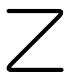
\includegraphics[keepaspectratio]{images/part002_816cd56c.jpg}}

（VI, p.~271, th. 1）（我们在 VI, p.~271 已把它记作 \(u(\mathrm{D})\) ），则以 \(\alpha_{n}\lambda^{n+p}\) 为通项的复数项级数对 \(\lambda \neq 0\) 不一定收敛，而且即使它对 \(\lambda\) 的某些值收敛，其和也不一定等于 U 的指示函数 \(u(\lambda)\) （VI, p.~291, exerc. 2）。若存在 C 中 0 的一个邻域，使得以 \(\alpha_{n}\lambda^{n+p}\) 为通项的级数在其上绝对收敛且其和等于指示函数 \(u(\lambda)\) ，则我们称复合算子 U 为正则的 \(^{1}\) 。把 VI, p.~278 的公式 (27) 应用于函数 \(e^{\lambda x}\) ，取 h = 0；由于 \(\mathrm{D}^{m}(e^{\lambda x}) = \lambda^{m} e^{\lambda x}\) ，有 \(U_{0}^{\xi}\left(\mathrm{D}^{m}(e^{\lambda x})\right) = \lambda^{m} u(\lambda)\) ；由此得出，对每个复数 \(\lambda\) （满足 \(u(\lambda) \neq 0\) 的）

\[
\frac {\lambda^ {p} e ^ {\lambda x}}{u (\lambda)} = \sum_ {m = 0} ^ {n} u _ {m} (x) \frac {\lambda^ {m}}{m !} - \frac {\lambda^ {n + 1}}{u (\lambda)} U _ {0} ^ {\xi} \left(\int_ {0} ^ {\xi - x} \frac {1}{n !} u _ {n} (x + \eta) e ^ {\lambda (\xi - \eta)} d \eta\right)\tag{31}
\]

特别地，对 \(x = 0\) ，有

\[
\frac {\lambda^ {p}}{u (\lambda)} = \sum_ {m = 0} ^ {n} \beta_ {m} \frac {\lambda^ {m}}{m !} - \frac {\lambda^ {n + 1}}{u (\lambda)} U _ {0} ^ {\xi} \left(\int_ {0} ^ {\xi} \frac {1}{n !} u _ {n} (\eta) e ^ {\lambda (\xi - \eta)} d \eta\right)\tag{32}
\]

其中 \(\beta_{m} = u_{m}(0)\) 。

若 \(U\) 是正则算子，则对一切 \(\lambda \in \mathbf{C}\) （使幂级数 \(u(\lambda) = \sum_{n=0}^{\infty} \alpha_n \lambda^{n+p}\) 与 \(\sum_{n=0}^{\infty} \beta_n \frac{\lambda^n}{n!}\) 绝对收敛者）\(^2\) ，由公式 (16) 及两个绝对收敛级数的乘积公式（Gen.~Top., VIII, p.~115, prop. 1），有

\[
{\frac {\lambda^ {p}}{u (\lambda)}} = \sum_ {n = 0} ^ {\infty} \beta_ {n} {\frac {\lambda^ {n}}{n !}}.\tag{33}
\]

同样，由于 \(e^{\lambda x}\) 的泰勒展开对每个 \(\lambda \in \mathbf{C}\) 和每个 \(x \in \mathbf{C}\) 都绝对收敛（III, p.~106），（由公式 (6) （VI, p.~273）与 (16) （VI, p.~274））对所考虑的一切值和一切 \(x \in \mathbf{C}\) 也有

\[
\frac {\lambda^ {p} e ^ {\lambda x}}{u (\lambda)} = \sum_ {n = 0} ^ {\infty} u _ {n} (x) \frac {\lambda^ {n}}{n !}.\tag{34}
\]

注. 可以利用公式 (33) （相应地 (34)），借助下面关于幂级数的引理来计算诸 \(\beta_{n}\) （相应地诸 \(u_{n}(x)\) ）：

引理. 若两个幂级数 \(\sum_{n=0}^{\infty} c_n \lambda^n\) 、\(\sum_{n=0}^{\infty} d_n \lambda^n\) 在 0 的某个邻域内的一切 \(\lambda\) 处绝对收敛，且若 \(\sum_{n=0}^{\infty} c_n \lambda^n = \sum_{n=0}^{\infty} d_n \lambda^n\) 对这些 \(\lambda\) 的值成立，则 \(c_n = d_n\) （对一切整数 \(n \geqslant 0^3\) ）。

若用任何方法能找到一个在 0 的某个邻域上收敛于 \(\lambda^p / u(\lambda)\) 的幂级数，则该级数的系数必然等于诸 \(\beta_n / n!\) 。在下面各例中我们就要应用这个方法。

例. 1) 若 \(U\) 是恒等映射，则有 \(u(\lambda) = 1\) ，且显然算子 \(U\) 是正则的；由于 \(u_{n}(x) = x^{n}\) ，令 \(t = \xi - \eta\) ，VI, p.~278 的公式 (27) 可以写成

\[
f (x + h) = \sum_ {n = 0} ^ {\infty} \frac {1}{m !} f ^ {(m)} (h) x ^ {m} + \int_ {h} ^ {x + h} f ^ {(n + 1)} (t) \frac {(x + h - t) ^ {n}}{n !} d t
\]

也就是说，它归结为泰勒公式（II, p.~62）。

\begin{enumerate}
\def\labelenumi{\arabic{enumi})}
\setcounter{enumi}{1}
\tightlist
\item
  我们取 U 为这样的复合算子：它把定义在 \(R_{+}\) 上的每个函数 f 对应到函数 \(x \mapsto f(x + 1) - f(x)\) ；于是
\end{enumerate}

\[
U _ {x} ^ {\xi} (f (\xi)) = f (x + 1) - f (x);
\]

我们已看到（VI, p.~275），U 在 C{[}X{]} 上的限制等于 \(e^{D}-1\) 。另一方面，由于 \(u(\lambda)=e^{\lambda}-1\) ，算子 U 是正则的；我们将看到（VI, p.~288）如何确定伯努利数 \(b_{n}\) ，办法是把 \(\frac{\lambda}{e^{\lambda}-1}\) 展开为收敛的幂级数。把 VI, p.~278 的公式 (27) 应用于一个函数 f 的原函数（该函数有连续的 \(n^{th}\) 阶导数，在 \(R_{+}\) 上），就得到

\[
\begin{array}{l} f (x + h) = \int_ {h} ^ {h + 1} f (t) d t \\ \qquad + \sum_ {m = 1} ^ {n} \frac {1}{m !} \mathrm{B} _ {m} (x) \left(f ^ {(m - 1)} (h + 1) - f ^ {(m - 1)} (h)\right) + \mathrm{R} _ {n} (x, h) \end{array}\tag{35}
\]

\[
\begin{array}{l} \mathrm{R} _ {n} (x, h) = - \int_ {0} ^ {1 - x} \frac {\mathrm{B} _ {n} (x + \eta)}{n !} f ^ {(n)} (h + 1 - \eta) d \eta \\ \qquad \qquad + \int_ {0} ^ {- x} \frac {\mathrm{B} _ {n} (x + \eta)}{n !} f ^ {(n)} (h - \eta) d \eta . \end{array}\tag{36}
\]

*3) 设 \(\mathbf{E}\) 是由函数 \(f\) （在 \(\mathbf{R}\) 上定义且连续、并使积分 \(\int_{-\infty}^{+\infty} f(x + \xi)e^{-\xi^2 / 2}d\xi\) 对一切 \(x \geqslant 0\) 收敛的）所组成的向量空间。算子 \(\mathrm{U}\) 由

\[
U _ {x} ^ {\xi} (f (\xi)) = \frac {1}{\sqrt {2 \pi}} \int_ {- \infty} ^ {+ \infty} e ^ {- \xi^ {2} / 2} f (x + \xi) d \xi
\]

定义，它这时定义在 E 上且显然是一个复合算子。空间 E 包含所有指数函数 \(e^{\lambda x}\) （ \(\lambda\) 为任意复数），并且有

\[
\begin{array}{l} u (\lambda) = \frac {1}{\sqrt {2 \pi}} \int_ {- \infty} ^ {+ \infty} e ^ {- (\xi^ {2} / 2) + \lambda \xi} d \xi \\ = \frac {1}{\sqrt {2 \pi}} e ^ {\lambda^ {2} / 2} \int_ {- \infty} ^ {+ \infty} e ^ {- (\xi - \lambda) ^ {2} / 2} d \xi = e ^ {\lambda^ {2} / 2} \end{array}
\]

（参见 III, p.~120, exerc. 24 及 VII, p.~313, 公式 (22)）。有 \(n! \alpha_n = U_0^\xi (\xi^n) = \frac{1}{\sqrt{2\pi}} \int_{-\infty}^{+\infty} e^{-\xi^2 / 2} \xi^n d\xi\) 。对每个整数 \(n\) 可以写

\[
\sum_ {k = 0} ^ {n} \int_ {- \infty} ^ {+ \infty} \frac {| \lambda \xi | ^ {k}}{k !} e ^ {- \xi^ {2} / 2} d \xi \leqslant 2 \int_ {0} ^ {+ \infty} e ^ {- (\xi^ {2} / 2) + | \lambda | \xi} d \xi .
\]

于是级数 \(\sum_{n=0}^{\infty}e^{-\xi^{2}/2}\frac{(\lambda\xi)^{n}}{n!}\) 可以在 R 上逐项积分（II, p.~72, cor. 1），这就证明级数 \(\sum_{n=0}^{\infty}\alpha_{n}\lambda^{n}\) 对每个 \(\lambda\in C\) 绝对收敛，且其和等于 \(u(\lambda)=e^{\lambda^{2}/2}=\sum_{n=0}^{\infty}\frac{\lambda^{2n}}{2^{n}n!}\) ；因而算子 U 是正则的。应用上述引理可知，有 \(\alpha_{2n}=1/2^{n}n!\) ，\(\alpha_{2n+1}=0\) （对每个 \(n\geqslant0\) ）；于是算子 U 是 0 阶的。有

\[
\frac {1}{u (\lambda)} = e ^ {- \lambda^ {2} / 2} = \sum_ {n = 0} ^ {\infty} \frac {(- 1) ^ {n} \lambda^ {2 n}}{2 ^ {n} n !},
\]

该级数对每个 \(\lambda \in \mathbf{C}\) 绝对收敛；再次应用该引理可知 \(\beta_{2n} = \frac{(-1)^n}{2^n}\frac{(2n)!}{n!}\) ，\(\beta_{2n+1} = 0\) ；此外，级数 \(\sum_{n=0}^{\infty}\frac{\lambda^n}{n!} u_n(x)\) 对每个 \(\lambda \in \mathbf{C}\) 和每个 \(x \in \mathbf{R}\) 绝对收敛，并且有

\[
\sum_ {n = 0} ^ {\infty} \frac {\lambda^ {n}}{n !} u _ {n} (x) = \exp \left(- \frac {\lambda^ {2}}{2} + \lambda x\right) = \exp \left(\frac {x ^ {2}}{2}\right) \exp \left(- \frac {1}{2} (\lambda - x) ^ {2}\right).
\]

把泰勒公式应用于函数 \(\exp(-x^2/2)\) ，就得到多项式 \(u_n(x)\) 的下列表达式：

\[
u _ {n} (x) = (- 1) ^ {n} e ^ {x ^ {2} / 2} \frac {d ^ {n}}{d x ^ {n}} (e ^ {- x ^ {2} / 2}).
\]

这个多项式称为 n 次埃尔米特多项式，常记作 \(\mathrm{H}_{n}(x)\) 。VI, p.~273 的公式 (7)、(8) 和 (9) 在这里给出

\[
\frac {d \mathrm{H} _ {n}}{d x} = n \mathrm{H} _ {n - 1} (x)
\]

\[
\mathrm{H} _ {n} (x + y) = \sum_ {k = 0} ^ {n} {\binom {n} {k}} \mathrm{H} _ {n - k} (x)   y ^ {k}
\]

\[
\frac {1}{\sqrt {2 \pi}} \int_ {- \infty} ^ {+ \infty} e ^ {- \xi^ {2} / 2} \mathrm{H} _ {n} (x + \xi) d \xi = x ^ {n}
\]

而 VI, p.~278 的公式 (27) 在 \(h = 0\) 时成为

\[
\begin{array}{l} \sqrt {2 \pi} f (x) = \sum_ {m = 0} ^ {n} \left(\int_ {- \infty} ^ {+ \infty} e ^ {- \xi^ {2} / 2} f ^ {(m)} (\xi) d \xi\right) \frac {\mathrm{H} _ {m} (x)}{m !} \\ - \int_ {- \infty} ^ {+ \infty} d \xi \int_ {0} ^ {\xi} \frac {\mathrm{H} _ {n} (x + \eta)}{n !} e ^ {- (\xi + x) ^ {2} / 2} f ^ {(n + 1)} (x + \xi - \eta) d \eta . * \end{array}
\]

\subsection{欧拉–麦克劳林求和公式}

在 VI, p.~280 的公式 (35) 中，把 x 换成 0 ，h 换成 x；由于 \(\mathrm{B}_{m}(0)=b_{m}\) ，由 VI, p.~276 的关系 (24) 可知，对每个整数 p\textgreater0 可以写

\[
\begin{array}{l} f (x) = \int_ {x} ^ {x + 1} f (t) d t - \frac {1}{2} \big (f (x + 1) - f (x) \big) \\ \qquad + \sum_ {k = 1} ^ {p} \frac {b _ {2 k}}{(2 k) !} \left(f ^ {(2 k - 1)} (x + 1) - f ^ {(2 k - 1)} (x)\right) + \mathrm{R} _ {p} (x) \end{array}\tag{37}
\]

其中

\[
\mathrm{R} _ {p} (x) = - \frac {1}{(2 p + 1) !} \int_ {0} ^ {1} \mathrm{B} _ {2 p + 1} (t) f ^ {(2 p + 1)} (x + 1 - t) d t.\tag{38}
\]

在这个公式中，依次把 \(x\) 换成 \(x + 1, x + 2, \ldots, x + n\) ，并把所得的公式逐一合并；我们得到

\[
\left\{ \begin{array}{l} f (x) + f (x + 1) + \dots + f (x + n) \\ = \int_ {x} ^ {x + n + 1} f (t) d t - \frac {1}{2} \bigl (f (x + n + 1) - f (x) \bigr) \\ \quad + \sum_ {k = 1} ^ {p} \frac {b _ {2 k}}{(2 k) !} \bigl (f ^ {(2 k - 1)} (x + n + 1) - f ^ {(2 k - 1)} (x) \bigr) + \mathrm{T} _ {p} (x, n) \end{array} \right.\tag{39}
\]

其中

\[
\mathrm{T} _ {p} (x, n) = - \frac {1}{(2 p + 1) !} \int_ {0} ^ {1} \mathrm{B} _ {2 p + 1} (t) \left(\sum_ {k = 0} ^ {n} f ^ {(2 p + 1)} (x + k + 1 - t)\right) d t.\tag{40}
\]

这个公式中的余项 \(T_{p}(x,n)\) 可以改写成如下形式：用 \(\overline{\mathbf{B}}_{2p+1}(t)\) 表示以 1 为周期、等于 \(\mathbf{B}_{2p+1}(t)\) （在区间 {[}0, 1{[} 上）的周期函数。则

\[
\int_ {0} ^ {1} \mathrm{B} _ {2 p + 1} (t) f ^ {(2 p + 1)} (x + k + 1 - t) d t = \int_ {k} ^ {k + 1} \overline {{\mathrm{B}}} _ {2 p + 1} (1 - s) f ^ {(2 p + 1)} (x + s) d s
\]

因而

\[
\mathrm{T} _ {p} (x, n) = - \frac {1}{(2 p + 1) !} \int_ {0} ^ {n + 1} \overline {{\mathrm{B}}} _ {2 p + 1} (1 - s) f ^ {(2 p + 1)} (x + s) d s.\tag{41}
\]

公式 (39) 称为欧拉–麦克劳林求和公式；它适用于有连续的 \((2p+1)^{th}\) 阶导数（在区间 \([x_{0},+\infty[\) 上）的每个复值函数，对每个 \(x\geqslant x_{0}\) 都成立。我们将看到（VI, p.~288）如何估计这个公式中余项 \(T_{p}(x,n)\) 的界。

\section{三角函数与伯努利数的欧拉展开}

\subsection{\texorpdfstring{\(\cot z\) 的欧拉展开}{cot z 的欧拉展开}}

由 VI, p.~275 的公式 (20)，诸数 \(b_{n} / n!\) 是 \(S / (e^{S} - 1)\) 的形式级数展开中的系数；我们将在本节中证明，函数 \(z / (e^{z} - 1)\) 在 \(\mathbf{C}\) 中 0 的某个邻域上等于一个绝对收敛的幂级数的和；于是由 VI, p.~280 的引理可知，该级数的系数就是诸数 \(b_{n} / n!\) ，由此我们将导出伯努利数 \(b_{n}\) 的估计式。

首先我们注意

\[
{\frac {z}{e ^ {z} - 1}} = - {\frac {z}{2}} + {\frac {z}{2}} {\frac {e ^ {z} + 1}{e ^ {z} - 1}} = - {\frac {z}{2}} + {\frac {i z}{2}} \cot {\frac {i z}{2}}.\tag{1}
\]

下面我们将得到 \(\cot z\) 的一个级数展开，它对每个 \(z\) （只要不是 \(\pi\) 的整数倍）都成立。

命题 1. 对每个复数 \(z\) 和每个整数 \(n\) ，有

\[
\sin n z = 2 ^ {n - 1} \sin z \sin \left(z + \frac {\pi}{n}\right) \sin \left(z + \frac {2 \pi}{n}\right) \dots \sin \left(z + \frac {(n - 1) \pi}{n}\right).\tag{2}
\]

事实上，可以写

\[
\begin{array}{l} \sin n z = \frac {e ^ {n i z} - e ^ {- n i z}}{2 i} = \frac {e ^ {- n i z} (e ^ {2 n i z} - 1)}{2 i} \\ \quad = \frac {e ^ {- n i z} (e ^ {2 i z} - 1) (e ^ {2 i z} - e ^ {- 2 i \pi / n}) \dots (e ^ {2 i z} - e ^ {- 2 (n - 1) i \pi / n})}{2 i} \\ \quad = A \sin z \sin \left(z + \frac {\pi}{n}\right) \sin \left(z + \frac {2 \pi}{n}\right) \dots \sin \left(z + \frac {(n - 1) \pi}{n}\right) \end{array}
\]

其中

\[
\mathrm{A} = (2 i) ^ {n - 1} e ^ {- \frac {i \pi}{n} (1 + 2 + \dots + (n - 1))} = (2 i) ^ {n - 1} e ^ {- i (n - 1) \frac {\pi}{2}} = 2 ^ {n - 1}.
\]

推论 1. 对每个整数 n ，有

\[
\sin \frac {\pi}{n} \sin \frac {2 \pi}{n} \dots \sin \frac {(n - 1) \pi}{n} = \frac {n}{2 ^ {n - 1}}.\tag{3}
\]

只需把 (2) 的两边除以 \(\sin z\) 并让 z 趋于 0 。

推论 2. 对每个奇整数 \(n = 2m + 1\) 以及每个使 nz 不是 \(\pi\) 整数倍的复数 z ，有

\[
\cot n z = (- 1) ^ {m} \cot z \cot \left(z + \frac {\pi}{n}\right) \dots \cot \left(z + \frac {(n - 1) \pi}{n}\right).\tag{4}
\]

事实上，\(\sin n\left(z + \frac{\pi}{2}\right) = \sin \left(nz + \frac{\pi}{2} + m\pi\right) = (-1)^m\cos nz\) ，由此，在 (2) 中把 \(z\) 换成 \(z + \frac{\pi}{2}\) ，

\[
\cos n z = (- 1) ^ {m} 2 ^ {n - 1} \cos z \cos \left(z + \frac {\pi}{n}\right) \dots \cos \left(z + \frac {(n - 1) \pi}{n}\right)\tag{5}
\]

当 \(\sin nz \neq 0\) 时，把公式 (2) 与 (5) 逐项相除即得 (4)。

在后面我们总假设 \(n = 2m + 1\) 是奇整数；公式 (4) 也可以写成

\[
\cot n z = (- 1) ^ {m} \prod_ {k = - m} ^ {m} \cot \left(z - \frac {k \pi}{n}\right).
\]

因为，有

\[
\cot \left(z - \frac {k \pi}{n}\right) = \frac {1 + \tan z \tan \frac {k \pi}{n}}{\tan z - \tan \frac {k \pi}{n}}
\]

（对 \(\tan z\) 有限的情形）；于是 \(\cot nz\) 是 \(u = \tan z\) 的有理函数，其分子次数为 n - 1，分母次数为 n 且以 \(\tan k\pi/n\) 这 n 个数为单根；把它分解为简单分式即得

\[
\cot n z = \sum_ {k = - m} ^ {m} \frac {\mathrm{A} _ {k}}{u - \tan \frac {k \pi}{n}}\tag{6}
\]

其中

\[
\begin{array}{l}\mathrm{A} _ {k} = \lim _ {z \rightarrow k \pi / n} \cot n z \left(\tan z - \tan \frac {k \pi}{n}\right) = \lim _ {z \rightarrow k \pi / n} \frac {\cos n z}{\sin n z} \frac {\sin \left(z - \frac {k \pi}{n}\right)}{\cos z \cos \frac {k \pi}{n}}\\= \lim _ {h \rightarrow 0} \frac {\cos n h}{\cos \frac {k \pi}{n} \cos \left(h + \frac {k \pi}{n}\right)} \frac {\sin h}{\sin n h} = \frac {1}{n \cos^ {2} \frac {k \pi}{n}}\end{array}
\]

于是，把 (6) 中对应于 k = 0 的项单独分出，把对应于 k 的相反值的诸项合并，并把 z 换成 z/n ，

\[
\cot z = \frac {1}{n \tan \frac {z}{n}} + \sum_ {k = 1} ^ {m} \frac {2 n \tan \frac {z}{n}}{\cos^ {2} \frac {k \pi}{n} \left(n \tan \frac {z}{n}\right) ^ {2} - \left(n \sin \frac {k \pi}{n}\right) ^ {2}}\tag{7}
\]

它对每个复数 \(z\) （不是 \(\pi / 2\) 的整数倍的）成立。可以把这个公式写成

\[
\cot z = \frac {1}{n \tan \frac {z}{n}} + \sum_ {k = 1} ^ {\infty} v _ {k} (n, z)
\]

其中 \(v_{k}(n,z) = 0\) （对 \(k > m\) ），而

\[
v _ {k} (n, z) = \frac {2 n \tan \frac {z}{n}}{\cos^ {2} \frac {k \pi}{n} \left(n \tan \frac {z}{n}\right) ^ {2} - \left(n \sin \frac {k \pi}{n}\right) ^ {2}}
\]

对 \(1 \leqslant k \leqslant m\) 。我们将看到，对每个包含于 C 的紧子集 K 中的 \(z\) （K 不含 \(\pi\) 的任何整数倍），以及每个充分大的奇数 \(n\) ，以 \(v_{k}(n,z)\) 为通项的级数正规收敛。事实上，当 \(n\) 趋于 \(+\infty\) 时，\(\tan \frac{z}{n}\) 在 K 上一致趋于 \(\frac{z}{n}\) ，故存在数 M \textgreater{} 0 ，使得 \(\left| n \tan \frac{z}{n} \right| \leqslant M\) （对每个充分大的 \(m\) 和每个 \(z \in K\) ）。另一方面，对 \(0 \leqslant x \leqslant \pi/2\) 有 \(\sin x/x \geqslant 1 - \frac{x^2}{6} \geqslant \frac{1}{2}\) ，故对 \(1 \leqslant k \leqslant m\) 有 \(n \sin \frac{k\pi}{n} \geqslant k\pi/2\) ；因此，当 \(m\) 充分大时，对每个整数 \(k\) （满足 \(k\pi / 2 > \mathbf{M}\) 的）有 \(|v_k(n, z)| \leqslant \frac{8\mathbf{M}}{k^2\pi^2 - 4\mathbf{M}^2}\) ，这就证明了我们的断言。对固定的 \(k\) ，\(v_k(n, z)\) （在 \(\mathbf{K}\) 上一致）趋于 \(\frac{2z}{z^2 - k^2\pi^2}\) （当 \(n\) 趋于 \(+\infty\) 时）。于是：

定理 1. 对每个不是 \(\pi\) 整数倍的复数 z ，有

\[
\cot z = \frac {1}{z} + \sum_ {n = 1} ^ {\infty} \frac {2 z}{z ^ {2} - n ^ {2} \pi^ {2}}\tag{8}
\]

右端的级数在每个紧子集 \(K \subset C\) （不含 \(\pi\) 的任何整数倍）上正规收敛（\(\cot z\) 的欧拉展开）。

\subsection{sin z 的欧拉展开}

对每个奇整数 \(n = 2m + 1\) 和复数 \(z\) ，VI, p.~283 的公式 (2) 可以写成

\[
\begin{array}{l} \sin n z = (- 1) ^ {m}   2 ^ {n - 1}   \prod_ {k = - m} ^ {m}   \sin \left(z - \frac {k \pi}{n}\right) \\ = (- 1) ^ {m}   2 ^ {n - 1}   \sin z   \prod_ {k = 1} ^ {m}   \sin \left(z - \frac {k \pi}{n}\right) \sin \left(z + \frac {k \pi}{n}\right). \end{array}
\]

现在，有 \(\sin\left(z-\frac{k\pi}{n}\right)\sin\left(z+\frac{k\pi}{n}\right)=\sin^{2}z-\sin^{2}\frac{k\pi}{n}\) ，并且由 (3) （VI, p.~284）有 \(\prod_{k=1}^{m}\sin^{2}\frac{k\pi}{n}=\frac{n}{2^{n-1}}\) ，于是，把 \(z\) 换成 \(z/n\) ，

\[
\sin z = n \sin \frac {z}{n} \prod_ {k = 1} ^ {m} \left(1 - \frac {\sin^ {2} \frac {z}{n}}{\sin^ {2} \frac {k \pi}{n}}\right).\tag{9}
\]

可以把这个公式写成 \(\sin z = n\sin \frac{z}{n}\prod_{k = 1}^{m}\big(1 - w_k(n,z)\big)\) ，其中 \(w_{k}(n,z) = 0\) （对 \(k > m\) ），而 \(w_{k}(n,z) = \frac{\sin^{2}\frac{z}{n}}{\sin^{2}\frac{k\pi}{n}}\) （对 \(1\leqslant k\leqslant m\) ）。我们将看到，对每个 \(z\) （属于某个紧子集 \(\mathbf{K}\) ，\(\mathbf{C}\) 的）以及奇数 \(n\) ，以 \(w_{k}(n,z)\) 为通项的级数正规收敛。事实上，当 \(n\) 趋于 \(+\infty\) 时，\(n\sin \frac{z}{n}\) 一致趋于 \(z\) （在 \(\mathbf{K}\) 上），故存在数 \(\mathbf{M} > 0\) ，使得 \(\left|n\sin \frac{z}{n}\right|\leqslant \mathbf{M}\) （对每个整数 \(m\) 和每个 \(z\in \mathbf{K}\) ）。此外，我们在 VI, p.~286 定理 1 的证明中已经看到，对

\(1 \leqslant k \leqslant m\) 有 \(n \sin \frac{k\pi}{n} \geqslant \frac{k\pi}{2}\) ；于是对每个整数 \(k\) （满足 \(k\pi/2 \geqslant M\) 的）有 \(|w_k(n, z)| \leqslant 4M^2/k^2\pi^2\) ，这就证明了我们的断言。由于对每个固定的 \(k\) ，\(w_k(n, z)\) （在 K 上一致）趋于 \(z^2/k^2\pi^2\) （当 \(n\) 趋于 \(+\infty\) 时），可以看出：

定理 2. 对每个复数 \(z\) ，有

\[
\sin z = z \prod_ {n = 1} ^ {\infty} \left(1 - \frac {z ^ {2}}{n ^ {2} \pi^ {2}}\right)\tag{10}
\]

右端的无穷乘积在 C 的每个紧子集上绝对且一致收敛（\(\sin z\) 的欧拉展开）。

\subsection{在伯努利数上的应用}

VI, p.~286 的定理 1 表明，对 \(0 \leqslant x < \pi\) ，以 \(\frac{2x}{n^2\pi^2 - x^2} \geqslant 0\) 为通项的级数收敛。另一方面，对每个复数 \(z\) （满足 \(|z| < \pi\) 的），可以写成

\[
{\frac {2 z}{n ^ {2} \pi^ {2} - z ^ {2}}} = {\frac {2 z}{n ^ {2} \pi^ {2}}} \sum_ {k = 0} ^ {\infty} {\frac {z ^ {2 k}}{n ^ {2 k} \pi^ {2 k}}}
\]

右端的级数绝对收敛。我们将由此推出，“二重”级数

\[
\sum_ {n = 1} ^ {\infty} \sum_ {k = 1} ^ {\infty} \frac {- 2 z ^ {2 k - 1}}{n ^ {2 k} \pi^ {2 k}}\tag{11}
\]

在开圆盘 \(|z| < \pi\) 中绝对收敛，在含于此圆盘的每个紧集上正规收敛，且其和为 \(\cot z - \frac{1}{z}\) 。事实上，对 \(|z| \leqslant a < \pi\) ，(11) 的通项的绝对值至多等于 \(2a^{2k-1}/n^{2k}\pi^{2k}\) ，而项 \(2a^{2k-1}/n^{2k}\pi^{2k}\) 中任意有限多个之和小于有限数 \(\sum_{n=1}^{\infty} \frac{2a}{n^2\pi^2 - a^2}\) ；先对 \(k\) 求和、再对 \(n\) 求和，即可看出级数 (11) 的和等于 \(\sum_{n=1}^{\infty} \frac{2z}{z^2 - n^2\pi^2}\) ，这就证明了我们的结论。

现在若把级数 (11) 先对 \(n\) 求和、再对 \(k\) 求和，就得到恒等式（对 \(|z| < \pi\) ）

\[
\cot z - \frac {1}{z} = - 2 \sum_ {k = 1} ^ {\infty} \frac {S _ {2 k}}{\pi^ {2 k}} z ^ {2 k - 1}\tag{12}
\]

其中我们置 \(S_{k} = \sum_{n=1}^{\infty} \frac{1}{n^{k}}\) 。于是由 (1) （VI, p.~283）得到，对 \(|z| < 2\pi\)

\[
\frac {z}{e ^ {z} - 1} = 1 - \frac {z}{2} + \sum_ {n = 1} ^ {\infty} \frac {(- 1) ^ {n - 1} S _ {2 n}}{2 ^ {2 n - 1} \pi^ {2 n}} z ^ {2 n}\tag{13}
\]

由此得到公式

\[
b _ {2 n} = (- 1) ^ {n - 1} (2 n)! \frac {2 \mathrm{S} _ {2 n}}{(2 \pi) ^ {2 n}} \quad \text {   for   } n \geqslant 1,\tag{14}
\]

这个公式特别表明数 \(S_{2n} / \pi^{2n}\) 是有理数。显然 \(S_{k + 1} \leqslant S_k\) ，故对每个整数 \(k \geqslant 2\) 有 \(S_k \leqslant S_2 = \pi^2 / 6 \leqslant 2\) ；由 (14) 可推出伯努利数的下列不等式

\[
\frac {2 (2 n) !}{(2 \pi) ^ {2 n}} \leqslant | b _ {2 n} | \leqslant 4 \frac {(2 n) !}{(2 \pi) ^ {2 n}} \quad \text {   for   } n \geqslant 1.\tag{15}
\]

由这些不等式可以推出伯努利多项式 \(\mathrm{B}_n(x) = \sum_{k=0}^{n}\binom{n}{k}b_kx^{n - k}\) 的一个估计式；特别地，对 \(0 \leqslant x \leqslant 1\) 有

\[
\left| \mathrm{B} _ {n} (x) \right| \leqslant 4 \sum_ {k = 0} ^ {n} \binom {n} {k} \frac {k !}{(2 \pi) ^ {k}} = 4 \frac {n !}{(2 \pi) ^ {n}} \sum_ {k = 0} ^ {n} \frac {(2 \pi) ^ {k}}{k !} \leqslant 4 e ^ {2 \pi} \frac {n !}{(2 \pi) ^ {n}}.\tag{16}
\]

\section{欧拉–麦克劳林求和公式余项的估计}

\subsection{欧拉–麦克劳林求和公式余项的估计}

在 (16) 中对区间 \([0, 1]\) 上的伯努利多项式得到的估计式，使我们能容易地估计欧拉–麦克劳林求和公式（VI, p.~282，公式 (39)）的余项 \(T_{p}(x, n)\) ：

\[
\left\{ \begin{array}{l} f (x) + f (x + 1) + \dots + f (x + n) \\ = \int_ {x} ^ {x + n + 1} f (t) d t - \frac {1}{2} \bigl (f (x + n + 1) - f (x) \bigr) \\ \qquad + \sum_ {k = 1} ^ {p} \frac {b _ {2 k}}{(2 k) !} \bigl (f ^ {(2 k - 1)} (x + n + 1) - f ^ {(2 k - 1)} (x) \bigr) + T _ {p} (x, n). \end{array} \right.\tag{1}
\]

事实上，有（VI, p.~283，公式 (41)）

\[
\mathrm{T} _ {p} (x, n) = - \frac {1}{(2 p + 1) !} \int_ {0} ^ {n + 1} \overline {{\mathrm{B}}} _ {2 p + 1} (1 - s) f ^ {(2 p + 1)} (x + s) d s\tag{2}
\]

其中 \(\overline{\mathbf{B}}_{2p + 1}(t)\) 是以 1 为周期、等于 \(\mathrm{B}_{2p + 1}(t)\) （在区间 {[}0, 1{[} 上）的周期函数。VI, p.~288 的公式 (16) 表明

\[
\left| \overline {{{{\mathrm{B}}}}} _ {2 p + 1} (t) \right| \leqslant 4 e ^ {2 \pi} \frac {(2 p + 1) !}{(2 \pi) ^ {2 p + 1}}\tag{3}
\]

对一切 \(t \in R\) 成立，而应用中值公式即得估计式

\[
\left| \mathrm{T} _ {p} (x, n) \right| \leqslant \frac {4 e ^ {2 \pi}}{(2 \pi) ^ {2 p + 1}} \int_ {x} ^ {x + n + 1} \left| f ^ {(2 p + 1)} (t) \right| d t\tag{4}
\]

对 \(\mathrm{T}_p(x,n)\) 成立。

\subsection{在渐近展开上的应用}

欧拉–麦克劳林公式使我们对 V, p.~238 至 242 处理的问题——即求部分和 \(s_n = \sum_{m=0}^{n} g(m)\) （相应地，余和 \(r_n = \sum_{m=n+1}^{\infty} g(m)\) ）的渐近展开——能够（在最重要的情形）给出更完全的解，这里 \(g\) 是数量函数，\(> 0\) ，单调，定义在 \([0, +\infty[\) 上。

我们只限于 g 是 (H) 函数（V, p.~252）、相对于 \(e^{x}\) 的阶为 0 的情形；换句话说，有关系 \(g' \ll g\) ；由此推出，\(g^{(k+1)} \ll g^{(k)}\) （对每个整数 k \textgreater{} 0 ，只要各导数 \(g^{(h)}\) （阶 \(h \leqslant k\) 的）都不与常数等价；V, p.~232, prop. 7）。设 p 是这样一个整数：各导数 \(g^{(h)}\) （阶 \(h \leqslant 2p\) 的）都不与常数等价。先设以 \(g(n)\) 为通项的级数有无穷和，并区分几种情形：

\(1^{\circ}\left|g^{(2p - 1)}(n)\right|\) 趋于 \(+\infty\) （随 \(n\) ）；由假设，对 \(\left|g^{(2k - 1)}(n)\right|\) （\(1\leqslant k\leqslant p\) ）亦然；此外，由于 \(g^{(2p + 1)}\) 在 \(+\infty\) 的邻域上单调，VI, p.~289 的公式 (4) 给出 \(\mathrm{T}_p(0,n) = O\big(g^{(2p)}(n + 1)\big) = o\big(g^{(2p - 1)}(n + 1)\big)\) ；对 \(x = 0\) 应用欧拉–麦克劳林公式，就得到

\[
\begin{array}{l} s _ {n} = \sum_ {m = 0} ^ {n} g (m) = \int_ {0} ^ {n + 1} g (t) d t - \frac {1}{2} g (n + 1) \\ \qquad + \sum_ {k = 1} ^ {p} \frac {b _ {2 k}}{(2 k) !} g ^ {(2 k - 1)} (n + 1) + o \big (g ^ {(2 p - 1)} (n + 1) \big) \end{array}
\]

这个和中的每一项相对于前一项都是可忽略的；把每一项相对于一个比较尺度 E 展开，就得到 \(s_{n}\) 的一个渐近展开。

\(2^{\circ}\) 现在设对某个指标 \(q\) （满足 \(1 \leqslant q \leqslant p\) 的），\(\left|g^{(2q-1)}(n)\right|\) 趋于 \(+\infty\) （随 \(n\) ），但 \(g^{(2k-1)}(n)\) （对 \(k > q\) ）趋于 0 。由于 \(g^{(2p+1)}\) 在 \(+\infty\) 的邻域上单调，积分 \(\int_0^\infty \left|g^{(2p+1)}(u)\right| du\) 收敛，于是可以写成

\[
\begin{array}{l} s _ {n} = \sum_ {m = 0} ^ {n} g (m) = \int_ {0} ^ {n + 1} g (t) d t - \frac {1}{2} g (n + 1) + \sum_ {k = 1} ^ {q} \frac {b _ {2 k}}{(2 k) !} g ^ {(2 k - 1)} (n + 1) + C \\ \qquad + \sum_ {k = q + 1} ^ {p} \frac {b _ {2 k}}{(2 k) !} g ^ {(2 k - 1)} (n + 1) + o \big (g ^ {(2 p - 1)} (n + 1) \big) \end{array}
\]

其中 C 是常数：因为

\[
\int_ {n + 1} ^ {\infty} \left| g ^ {(2 p + 1)} (u) \right| d u = O \big (g ^ {(2 p)} (n + 1) \big) = o \big (g ^ {(2 p - 1)} (n + 1) \big).
\]

当 \(g(n)\) 本身趋于 0 时同一公式仍成立。最后，当以 \(g(n)\) 为通项的级数收敛时，对余和 \(r_n = \sum_{m=n+1}^{\infty} g(m)\) 有展开

\[
\begin{array}{l} r _ {n} = \sum_ {m = n + 1} ^ {\infty} g (m) = \int_ {n + 1} ^ {\infty} g (t) d t + \frac {1}{2} g (n + 1) \\ \qquad - \sum_ {k = 1} ^ {p} \frac {b _ {2 k}}{(2 k) !} g ^ {(2 k - 1)} (n + 1) + o \big (g ^ {(2 p - 1)} (n + 1) \big). \end{array}
\]

\setcounter{exercisegroup}{0}
\refstepcounter{exercisegroup}
\section*{第 \S\arabic{exercisegroup} 节习题}
\phantomsection
\addcontentsline{toc}{section}{第 \protect\S\arabic{exercisegroup} 节习题}

\begin{enumerate}
\def\labelenumi{\arabic{enumi})}
\tightlist
\item
  设 \(\mathbf{K}\) 是特征为 0 的域，\(U\) 和 \(V\) 是 \(\mathrm{K}[\mathrm{X}]\) 上的两个复合算子，且 \(W = VU = UV\) ；设 \((u_n), (v_n)(w_n)\) 是分别对应于 \(U, V, W\) 的阿佩尔多项式序列。证明：如果 \(p\) 是 \(U\) 的阶，那么
\end{enumerate}

\[
w _ {n} ^ {(p)} (\mathrm{X}) = \sum_ {k = 0} ^ {n} \binom {n} {k} v _ {n - k} (\mathrm{X}) V _ {0} (u _ {k})
\]

\[
w _ {n} (\mathrm{X} + \mathrm{Y}) = \sum_ {k = 0} ^ {n} \binom {n} {k} u _ {k} (\mathrm{X}) v _ {n - k} (\mathrm{Y}).
\]

\begin{enumerate}
\def\labelenumi{\arabic{enumi})}
\setcounter{enumi}{1}
\tightlist
\item
  设 \(\mathbf{E}\) 是 \(\mathbf{C}\) 上由函数 \(x^n\) （ \(n \in \mathbf{N}\) ）、\(e^{\lambda x}\) （ \(\lambda \in \mathbf{C}\) ，\(\lambda \neq 0\) ）与 \(|x + \mu|\) （ \(\mu \in \mathbf{R}\) ）生成的向量空间。
\end{enumerate}

\begin{enumerate}
\def\labelenumi{\alph{enumi})}
\item
  证明上述函数构成 E 的一组基。
\item
  设 \(U\) 是由下列条件在 \(\mathbf{E}\) 上定义的复合算子：\(U_0^\xi (\xi^n) = (n!)^2\) ，\(U(e^{\lambda x}) = e^{\lambda x}\) （对 \(\lambda \neq 0\) ），\(U(|x + \mu|) = |x + \mu|\) （对 \(\mu \in \mathbf{R}\) ）。指示函数 \(u(\lambda)\) 是常数 1 ，但以 \(n!\lambda^n\) 为通项的级数对任何值 \(\lambda \neq 0\) 都不收敛。
\item
  设 \(V\) 是由下列条件在 \(\mathbf{E}\) 上定义的复合算子：\(V(x^n) = x^n\) ，\(V(|x + \mu|) = |x + \mu|\) ，\(V(e^{\lambda x}) = 0\) （对 \(\lambda \neq 0\) ）；指示函数 \(v(\lambda)\) 当 \(\lambda = 0\) 时等于 1 ，当 \(\lambda \neq 0\) 时等于 0 ，因而异于级数 \(\sum_{n=0}^{\infty} \alpha_n \lambda^n\) 的和，其中 \(\alpha_n = V_0^\xi(\xi^n)/n!\) 。
\item
  设 W 是由下式在 E 上定义的复合算子
\end{enumerate}

\[
W (x ^ {n}) = x ^ {n}, \qquad W (e ^ {\lambda x}) = e ^ {\lambda x}, \qquad W (| x + \mu |) = e ^ {x + \mu};
\]

证明 \(VW \neq WV\) 。

\begin{enumerate}
\def\labelenumi{\arabic{enumi})}
\setcounter{enumi}{2}
\tightlist
\item
  设 K 是特征为 0 的域。称 K 上两个未定元 X, Y 的多项式所成的代数 \(K[X,Y]\) 的自同态 U 为复合算子，如果对每个多项式 \(f \in K[X,Y]\) ，置 \(g = U(f)\) 后有 \(g(X + S, Y + T) = U_{X,Y}(f(X + S, Y + T))\) ，其中 S 和 T 是另外两个未定元。
\end{enumerate}

\begin{enumerate}
\def\labelenumi{\alph{enumi})}
\item
  把 prop. 1 与 th. 1 推广到这些算子。由此导出公式 \(e^{\mathrm{S + T}} = e^{\mathrm{S}}e^{\mathrm{T}}\) 的一个新证明。
\item
  对形如 \(D_{X}^{p}D_{Y}^{q}u(D_{X},D_{Y})\) （其中形式级数 u 的常数项不为零）的复合算子，定义阿佩尔多项式 \(u_{mn}\) ，并推广 VI, p.~273 与 274 的 props. 4、5 和 6 。
\item
  特别考虑由 \(U(f(\mathrm{X},\mathrm{Y})) = f(\mathrm{X} + 1, \mathrm{Y} + 1) - f(\mathrm{X},\mathrm{Y} + 1) - f(\mathrm{X} + 1, \mathrm{Y}) + f(\mathrm{X},\mathrm{Y})\) 定义的复合算子 U ；对应于这个算子的阿佩尔多项式称为伯努利多项式，记作 \(B_{m,n}\) 。证明 \(\mathrm{B}_{m,n}(\mathrm{X},\mathrm{Y}) = \mathrm{B}_{m}(\mathrm{X})\mathrm{B}_{n}(\mathrm{Y})\) 。
\end{enumerate}

\setcounter{exercisegroup}{1}
\refstepcounter{exercisegroup}
\section*{第 \S\arabic{exercisegroup} 节习题}
\phantomsection
\addcontentsline{toc}{section}{第 \protect\S\arabic{exercisegroup} 节习题}

\begin{enumerate}
\def\labelenumi{\arabic{enumi})}
\tightlist
\item
  建立公式
\end{enumerate}

\[
\tan z = \sum_ {n = 1} ^ {\infty} (- 1) ^ {n - 1} 2 ^ {2 n} (2 ^ {2 n} - 1) b _ {2 n} \frac {z ^ {2 n - 1}}{(2 n) !}
\]

\[
\frac {1}{\sin z} = \frac {1}{z} + \sum_ {n = 1} ^ {\infty} (- 1) ^ {n - 1} 2 (2 ^ {2 n - 1} - 1) b _ {2 n} \frac {z ^ {2 n - 1}}{(2 n) !}
\]

其中右端的级数绝对收敛，第一个对 \(|z| < \frac{\pi}{2}\) ，第二个对 \(|z| < \pi\) （把 \(\tan z\) 与 \(1/\sin 2z\) 表成 \(\cot z\) 与 \(\cot 2z\) 的线性组合）。由此推出数 \(\frac{2^{2n}(2^{2n}-1)}{2n} b_{2n}\) 都是整数。（利用下述引理：若在两个绝对收敛级数 \(\sum_{n=0}^{\infty} \alpha_n \frac{z^n}{n!}\) 、\(\sum_{n=0}^{\infty} \beta_n \frac{z^n}{n!}\) 中系数 \(\alpha_n\) 与 \(\beta_n\) 都是整数，则在写成 \(\sum_{n=0}^{\infty} \gamma_n \frac{z^n}{n!}\) 形式的乘积中，诸 \(\gamma_n\) 都是整数。）

\begin{enumerate}
\def\labelenumi{\arabic{enumi})}
\setcounter{enumi}{1}
\tightlist
\item
  建立公式
\end{enumerate}

\[
(n - 1) \mathrm{B} _ {n} (\mathrm{X}) = n (\mathrm{X} - 1) \mathrm{B} _ {n - 1} (\mathrm{X}) - \sum_ {k = 0} ^ {n} \binom {n} {k} b _ {k}   \mathrm{B} _ {n - k} (\mathrm{X})
\]

（把级数 \(Se^{SX}/(e^{S}-1)\) 对 S 求导）。由此推出公式

\[
(2 n + 1) b _ {2 n} = - \sum_ {k = 1} ^ {n - 1} \binom {2 n} {2 k} b _ {2 k}   b _ {2 n - 2 k}
\]

它是关于伯努利数的。

\begin{enumerate}
\def\labelenumi{\arabic{enumi})}
\setcounter{enumi}{2}
\tightlist
\item
  证明：对每个整数 p \textgreater{} 1 ，
\end{enumerate}

\[
\mathrm{B} _ {n} \left(\frac {x}{p}\right) + \mathrm{B} _ {n} \left(\frac {x + 1}{p}\right) + \dots + \mathrm{B} _ {n} \left(\frac {x + p - 1}{p}\right) = \frac {1}{p ^ {n - 1}} \mathrm{B} _ {n} (\mathrm{X}).
\]

\begin{enumerate}
\def\labelenumi{\arabic{enumi})}
\setcounter{enumi}{3}
\tightlist
\item
  \begin{enumerate}
  \def\labelenumii{\alph{enumii})}
  \tightlist
  \item
    证明关系式
  \end{enumerate}
\end{enumerate}

\[
\mathrm{B} _ {n} (1 - \mathrm{X}) = (- 1) ^ {n} \mathrm{B} _ {n} (\mathrm{X})
\]

（利用事实：\(b_{2n - 1} = 0\) （对 \(n > 1\) ），以及关系式

\[
\mathrm{B} _ {n} (1 - \mathrm{X}) - \mathrm{B} _ {n} (- \mathrm{X}) = (- 1) ^ {n} n \mathrm{X} ^ {n - 1}.
\]

\begin{enumerate}
\def\labelenumi{\alph{enumi})}
\setcounter{enumi}{1}
\tightlist
\item
  证明
\end{enumerate}

\[
\mathrm{B} _ {n} \left(\frac {1}{2}\right) = b _ {n} \left(\frac {1}{2 ^ {n - 1}} - 1\right)
\]

（利用 exerc. 3）。

\begin{enumerate}
\def\labelenumi{\alph{enumi})}
\setcounter{enumi}{2}
\tightlist
\item
  证明：当 n 为偶数时，\(\mathrm{B}_{n}(\mathrm{X})\) 在 R 的区间 {[}0, 1{]} 中有两个根；而当 n 为奇数且 \textgreater{} 1 时，\(\mathrm{B}_{n}(\mathrm{X})\) 在点 0 、\(\frac{1}{2}\) 与 1 处有单根，且在 {[}0, 1{]} 的其他任何点处都不为零（利用 b) 及关系式 \(B_{n}^{\prime}=nB_{n-1}\) ）。
\end{enumerate}

\(d\) ) 由 \(c\) ) 推出：当 \(n\) 为偶数时，\(|\mathrm{B}_n(x)|\) 在区间 {[}0, 1{]} 上的最大值是 \(|b_n|\) ；而当 \(n\) 为奇数时，若 \(a_{n}\) 是 \(|\mathrm{B}_n(x)|\) 在 {[}0, 1{]} 上的最大值，则

\[
\frac {4}{n + 1} \left| b _ {n + 1} \right| \left(1 - \frac {1}{2 ^ {n}}\right) \leqslant a _ {n} \leqslant \frac {1}{2} n \left| b _ {n - 1} \right|
\]

（利用中值定理）。

\begin{enumerate}
\def\labelenumi{\arabic{enumi})}
\setcounter{enumi}{4}
\tightlist
\item
  若置 \(S_{n}(x) = \frac{1}{n + 1} (\mathrm{B}_{n + 1}(x) - \mathrm{B}_{n + 1}(0))\) ，则对每个整数 \(a > 0\) 有
\end{enumerate}

\[
\mathrm{S} _ {n} (a) = 1 ^ {n} + 2 ^ {n} + \dots + (a - 1) ^ {n}.
\]

\begin{enumerate}
\def\labelenumi{\alph{enumi})}
\item
  证明：对每个整数 \(n \geqslant 0\) 和每个整数 \(a > 0\) ，有 \(2\mathrm{S}_{2n + 1}(a) \equiv 0 \pmod{a}\) （考虑和 \(k^{2n + 1} + (a - k)^{2n + 1}\) ）。
\item
  设 \(r\) 和 \(s\) 是任意两个整数，证明
\end{enumerate}

\[
\mathrm{S} _ {n} (r s) \equiv s \mathrm{S} _ {n} (r) + n r \mathrm{S} _ {n - 1} (r) \mathrm{S} _ {1} (s) \pmod {r ^ {2}}.
\]

\begin{enumerate}
\def\labelenumi{\alph{enumi})}
\setcounter{enumi}{2}
\tightlist
\item
  设 p 是素数。证明：若 n 被 p-1 整除，则有 \(S_{n}(p) \equiv -1 \pmod{p}\) ；若 n 不被 p-1 整除，则 \(S_{n}(p) \equiv 0 \pmod{p}\) （若整数 g 不被 p 整除，注意 \(S_{n}(p) \equiv g^{n}S_{n}(p) \pmod{p}\) ）。
\end{enumerate}

\begin{enumerate}
\def\labelenumi{\arabic{enumi})}
\setcounter{enumi}{5}
\tightlist
\item
  \begin{enumerate}
  \def\labelenumii{\alph{enumii})}
  \tightlist
  \item
    设有理数 \(b_{n}\) 已由 VI, p.~275 的公式 (20) 定义，用 \(d_{n}\) 表示 \textgreater{} 0 的分母（即写成既约分数的 \(b_{n}\) 的分母）。证明 \(d_{n}\) 的任何素因子都不能 \(> n + 1\) （利用 VI, p.~276 的递推公式 (23)）。
  \end{enumerate}
\end{enumerate}

\begin{enumerate}
\def\labelenumi{\alph{enumi})}
\setcounter{enumi}{1}
\tightlist
\item
  证明：对每个整数 p \textgreater{} 0 和每个整数 n \textgreater{} 0 ，
\end{enumerate}

\[
\mathrm{S} _ {n} (p) = b _ {n} p + \binom {n} {1} \frac {p}{2} b _ {n - 1} p + \dots + \binom {n} {r} \frac {p ^ {r}}{r + 1} b _ {n - r} p + \dots + \frac {p ^ {n + 1}}{n + 1}.
\]

\begin{enumerate}
\def\labelenumi{\alph{enumi})}
\setcounter{enumi}{2}
\item
  由 b) 出发对 n 作递归，推出对每个素数 p ，把 \(S_{n}(p) - b_{n}p\) 写成既约分数时的分母不被 p 整除（注意 \(p^{r+1}\) 不能整除 \(r + 1\) ）。
\item
  由 c) 推出，数
\end{enumerate}

\[
b _ {n} - \sum_ {p} \frac {\mathrm{S} _ {n} (p)}{p}
\]

（其中 \(p\) 取遍素数集合 \(p \leqslant n + 1\) ，且 \(n\) 为偶数）是整数。由此推出

\[
b _ {2 n} + \sum_ {p} \frac {1}{p}
\]

（其中 \(p\) 取遍满足 \(p - 1\) 整除 \(2n\) 的素数集合）是整数（克劳森–冯·施陶特定理；利用 exerc. 5 c）。

* 7) 我们承认：对每个整数 \(a > 0\) ，整数集合 \(1 + ma\) （ \(m\) 取遍整数集 \(\geqslant 1\) ）中有无穷多个素数（这是狄利克雷关于算术数列的定理的一个特例）。

\begin{enumerate}
\def\labelenumi{\alph{enumi})}
\item
  设 n 是整数 \(\geqslant 1\) ，\(s \geqslant 1\) 是使 \(q = 1 + (2n + 1)!s\) 为素数的整数；证明：若 p 是素数且 p - 1 整除 2nq ，则 p - 1 必整除 2n （相反的情形将有 p - 1 = qd ，其中 d 是整数，从而 p 被 \(d + 1\) 整除）。
\item
  由 a) 推出：对每个整数 n \textgreater{} 0 ，存在无穷多个整数 m \textgreater{} n 使 \(b_{2m} - b_{2n}\) 是整数。*
\end{enumerate}

\begin{enumerate}
\def\labelenumi{\arabic{enumi})}
\setcounter{enumi}{7}
\item
  证明：对每个素数 \(p > 3\) ，把 \(\mathrm{S}_{2n}(p^k) - p^k b_{2n}\) 写成既约分数后，其分子被 \(p^{2k}\) 整除（按 exerc. 6 的方式论证）。
\item
  称有理数 \(r\) 是 \(p\) 进整数（Gen.~Top., III, p.~322, exerc. 23）（\(p\) 为素数），意思是当把 \(r\) 表成既约分数时其分母不被 \(p\) 整除；记 \(r \equiv 0 \pmod{p}\) 以表示 \(r/p\) 是 \(p\) 进整数这一事实，而 \(r \equiv r' \pmod{p}\) 按定义等价于 \(r - r' \equiv 0 \pmod{p}\) 。
\end{enumerate}

\begin{enumerate}
\def\labelenumi{\alph{enumi})}
\tightlist
\item
  设 \(m\) 是有理整数；函数 \(F_{m}(z) = \frac{m}{e^{mz} - 1} - \frac{1}{e^{z} - 1}\) 在 \(|z|\) 充分小时解析，因而可以写成在 0 的一个邻域上收敛的幂级数
\end{enumerate}

\[
\mathrm{F} _ {m} (z) = \sum_ {n = 1} ^ {\infty} (m ^ {n} - 1) \frac {b _ {n}}{n} \frac {z ^ {n - 1}}{(n - 1) !}.
\]

证明在 0 的一个邻域上也有

\[
\mathrm{F} _ {m} (z) = \sum_ {n = 0} ^ {\infty} c _ {n} (e ^ {z} - 1) ^ {n}
\]

其中 \(c_{n}\) 是 \(p\) 进整数；由此推出数 \(a_{n} = (m^{n} - 1)\frac{b_{n}}{n}\) 是 \(p\) 进整数；此外，有 \(a_{n + p - 1} \equiv a_{n} (\mathrm{mod.} p)\) 。

\[
\frac {b _ {n + p - 1}}{n + p - 1} \equiv \frac {b _ {n}}{n} \pmod {p}
\]

\begin{enumerate}
\def\labelenumi{\alph{enumi})}
\setcounter{enumi}{1}
\tightlist
\item
  由 a) 推出：若 \(p - 1\) 不整除 \(n\) ，则 \(b_{n} / n\) 是 \(p\) 进整数，并且有（库默尔同余）。（取 \(m\) 为 mod. \(p\) 类是 \(\mathbf{Z} / p\mathbf{Z}\) 的可逆元素所成乘法群的生成元的整数（Alg., VII. 12）。）
\end{enumerate}

\begin{enumerate}
\def\labelenumi{\arabic{enumi})}
\setcounter{enumi}{9}
\item
  用 exerc. 9 的记号，证明数 \(m^n a_n = m^n (m^n - 1)b_n / n\) 都是整数（把 \(F_m(z)\) 写成 \(e^z\) 的两个多项式之商）。由此推出（对偶数 \(n\) \(\geqslant 2\) ）：分母 \(\delta_n\) （既约形式的 \(b_n / n\) 的）满足：对每个整数 \(m\) （与 \(n\) 互素的）有 \(m^n \equiv 1\) (mod. \(\delta_n\) )。进而，若整数 \(d\) 满足 \(m^n \equiv 1\) (mod. \(d\) )（对每个整数 \(m\) ，与 \(n\) 互素的），则 \(d\) 整除 \(\delta_n\) （利用克劳森–冯·施陶特定理以及 \(\mathbf{Z} / d\mathbf{Z}\) 的乘法群的结构（Alg., VII. 12））。
\item
  \begin{enumerate}
  \def\labelenumii{\alph{enumii})}
  \tightlist
  \item
    设 p 是素数 \(\neq 2\) 。则下列性质等价：
  \end{enumerate}
\end{enumerate}

\(\alpha) b_n / n \not\equiv 0 \pmod{p}\) 对每个偶数 \(n\) （使 \(p - 1\) 不整除 \(n\) 的）。

\(\beta) b_n \not\equiv 0 \pmod{p}\) （对 \(n = 2, 4, 6, \ldots, p - 3\) ）。

（利用 exerc. 9b)。）

\begin{enumerate}
\def\labelenumi{\alph{enumi})}
\setcounter{enumi}{1}
\tightlist
\item
  若 \(p\) 等于 2 或满足 \(a\) ) 中的等价条件，则称 \(p\) 是正则素数；否则称为非正则素数。素数 2, 3, 5, 7, 11 是正则的；691 是非正则的。
\end{enumerate}

设 \(I\) 是非正则素数的一个有限集。设 \(n\) 是整数 \(\geqslant 2\) ，为 \(\prod_{q \in I} (q - 1)\) 的倍数

且使 \(|b_n / n| > 1\) （参看 VI, p.~288，公式 (15)）。设 \(p\) 是既约形式的 \(|b_n / n|\) 的分子的一个素因子。证明 \(p - 1\) 不整除 \(n\) ，因而 \(p\) 是非正则的。由此推出非正则素数的集合是无穷的。

\begin{enumerate}
\def\labelenumi{\arabic{enumi})}
\setcounter{enumi}{11}
\tightlist
\item
  对每个多项式 \(\mathbf{Q}\) （具有实系数且满足 \(\mathrm{Q}(0) = \mathrm{Q}(1)\) 的），用 \(\tilde{\mathbf{Q}}\) 表示 \(\mathbf{R}\) 上满足下列条件的连续函数：\(\tilde{\mathbf{Q}}(x) = \mathbf{Q}(x)\) （对 \(0 \leqslant x \leqslant 1\) ），且 \(\tilde{\mathbf{Q}}(x + 1) = \tilde{\mathbf{Q}}(x)\) （对每个 \(x \in \mathbf{R}\) ）。
\end{enumerate}

\begin{enumerate}
\def\labelenumi{\alph{enumi})}
\item
  对每个整数 \(m \geqslant 2\) ，伯努利多项式 \(B_{m}\) 是唯一的实系数多项式 Q ：次数为 m 、首项系数为 1 ，满足 \(\int_{0}^{1} Q(x) dx = 0\) 、\(Q(1) = Q(0)\) ，且使函数 \(\tilde{Q}\) 在 R 上 m - 2 次可导并有连续的 \((m - 2)^{nd}\) 阶导数。（对 m 作递归论证。）
\item
  证明：对 \(m \geqslant 1\) ，
\end{enumerate}

\[
\int_ {0} ^ {1} \mathrm{B} _ {m} (x) e ^ {- 2 \pi i n x} d x = \left\{ \begin{array}{c c c} 0 & \text {if} & n = 0 \\ - \frac {m !}{(2 \pi i n) ^ {m}} & \text {if} & n \neq 0 \end{array} \right. \text {on} \mathbf {Z}.
\]

* c) 由 b) 推出：对 \(0 \leqslant x \leqslant 1\) 和 \(m \geqslant 2\) ，有

\[
\mathrm{B} _ {m} (x) = - \frac {m !}{(2 \pi i) ^ {m}} \sum_ {n \in \mathbf {Z} - \{0 \}} \frac {e ^ {2 \pi i n x}}{n ^ {m}}
\]

级数正规收敛。*

\begin{enumerate}
\def\labelenumi{\arabic{enumi})}
\setcounter{enumi}{12}
\tightlist
\item
  设 \(f\) 是整数 \(\geqslant 1\) ，\(\chi\) 是定义在 \(\mathbf{Z}\) 上、取复值、且满足 \(\chi(x + f) = \chi(x)\) （对每个 \(x \in \mathbf{Z}\) ）的函数。若置
\end{enumerate}

\[
\hat {\chi} (y) = \frac {1}{f} \sum_ {x = 0} ^ {f - 1} \chi (x) e ^ {- 2 \pi i x y / f} \quad \text { for } y \in \mathbf {Z},
\]

则有

\[
\chi (x) = \sum_ {y = 0} ^ {f - 1} \hat {\chi} (y) e ^ {- 2 \pi i x y / f} \quad \text {   for   } x \in \mathbf {Z}.
\]

由 exerc. 12 推出：对每个整数 \(m \geqslant 2\) ，

\[
\sum_ {n \in \mathbf {Z} \backslash \{0 \}} \frac {\chi (n)}{n ^ {m}} = - \frac {(2 \pi i) ^ {m}}{m !} \sum_ {y = 0} ^ {f - 1} \hat {\chi} (y) \mathrm{B} _ {m} \left(\frac {y}{f}\right).
\]

例如，有

\[
1 - \frac {1}{3 ^ {3}} + \frac {1}{5 ^ {3}} - \dots + \frac {(- 1) ^ {n}}{(2 n + 1) ^ {3}} + \dots = \frac {\pi^ {3}}{3 2}.
\]

\setcounter{exercisegroup}{2}
\refstepcounter{exercisegroup}
\section*{第 \S\arabic{exercisegroup} 节习题}
\phantomsection
\addcontentsline{toc}{section}{第 \protect\S\arabic{exercisegroup} 节习题}

\begin{enumerate}
\def\labelenumi{\arabic{enumi})}
\tightlist
\item
  证明：若 \(f^{(2p + 1)}(t)\) 在区间 \([x, x + n + 1]\) 上单调，则欧拉–麦克劳林公式 VI, p.~288 （公式 (2)）的余项 \(\mathrm{T}_p(x, n)\) 与项
\end{enumerate}

\[
\frac {1}{(2 p + 2) !} b _ {2 p + 2} \left(f ^ {(2 p + 1)} (x + n + 1) - f ^ {(2 p + 1)} (x)\right)
\]

有相同的符号，且其绝对值至多等于该项的绝对值。

若假设 \(f^{(2p+2)}\) 连续（但符号任意），证明有

\[
\begin{array}{c} \left| T _ {p} (x, n) \right| \leqslant \frac {1}{(2 p + 2) !} \left| b _ {2 p + 2} \right| \Bigg (\left| f ^ {(2 p + 1)} (x + n + 1) - f ^ {(2 p + 1)} (x) \right| \\ \qquad \qquad \qquad \qquad \qquad \qquad \qquad \qquad \qquad + \int_ {x} ^ {x + n + 1} \left| f ^ {(2 p + 2)} (t) \right| d t \Bigg). \end{array}
\]

\begin{enumerate}
\def\labelenumi{\arabic{enumi})}
\setcounter{enumi}{1}
\tightlist
\item
  建立公式
\end{enumerate}

\[
\begin{array}{l} \frac {1}{2} f (x) - f (x + 1) + f (x + 2) - \dots - f (x + 2 n - 1) + \frac {1}{2} f (x + 2 n) \\ = \sum_ {k = 1} ^ {p} \frac {b _ {2 k}}{(2 k) !} (2 ^ {2 k} - 1) (f ^ {(2 k - 1)} (x + 2 n) - f ^ {(2 k - 1)} (x)) + V _ {p} (x, n) \end{array}
\]

其中

\[
\left| \mathrm{V} _ {p} (x, n) \right| \leqslant \frac {4 e ^ {2 \pi} \left(2 ^ {2 p + 1} + 1\right)}{(2 \pi) ^ {2 p + 1}} \int_ {x} ^ {x + 2 n} \left| f ^ {(2 p + 1)} (t) \right| d t
\]

（把欧拉–麦克劳林公式应用于 \(g(x) = f(2x)\) ）。

\begin{enumerate}
\def\labelenumi{\arabic{enumi})}
\setcounter{enumi}{2}
\tightlist
\item
  设 \(f\) 是有 \(2p + 1\) 阶连续导数（在区间 {[}0, 1{]} 上）的连续函数。建立公式
\end{enumerate}

\[
\begin{array}{l} \int_ {0} ^ {1} f (t) d t = \frac {1}{n} \left(\frac {1}{2} f (0) + f \left(\frac {1}{n}\right) + f \left(\frac {2}{n}\right) + \dots + f \left(\frac {n - 1}{n}\right) + \frac {1}{2} f (1)\right) \\ - \sum_ {k = 1} ^ {2 p} \frac {b _ {2 k}}{(2 k) !} \frac {1}{n ^ {2 k}} (f ^ {(2 k - 1)} (1) - f ^ {(2 k - 1)} (0)) + R _ {p} (n) \end{array}
\]

其中

\[
\left| \mathrm{R} _ {p} (n \right| \leqslant \frac {4 e ^ {2 \pi}}{(2 \pi) ^ {2 p + 1}} \frac {1}{n ^ {2 p + 1}} \int_ {0} ^ {1} \left| f ^ {(2 p + 1)} (t) \right| d t.
\]

\section*{历史注记（第五章与第六章）}
\phantomsection
\addcontentsline{toc}{section}{历史注记（第五章与第六章）}

（注意：罗马数字指本注记末尾所附的参考文献。）

不同阶的“无穷小”（或“无穷大”）之间的区分隐含地出现在微分学最早的著作中，例如费马的著作中；随着牛顿与莱布尼茨以及“高阶差分”理论的出现，它变得完全明确；而且人们很快就观察到，在最简单的情形，形如 \(f(x)/g(x)\) 的表达式在 f 与 g 都趋于 0 的点处的极限（或“真值”）由这些函数在所考虑点的邻域上的泰勒展开给出（“洛必达法则”，很可能属于约翰·伯努利）。

除初等情形外，从 XVII \(^{th}\) 世纪末起摆在数学家面前的主要的“渐近估计”问题，是当 n 很大时形如 \(\sum_{k=1}^{n} f(k)\) 的和的精确或近似计算；这种计算无论对插值法、对级数和的数值估计，还是对概率计算（其中诸如 n! 或 \(\binom{a}{n}\) 这类“大数的函数”起着占优的作用）都确实必不可少。早在牛顿，为了在 n 大时得到 \(\sum_{k=1}^{n} \frac{1}{a+k}\) 的近似值，就给出了一个方法，它（在这种特殊情形）归结为欧拉–麦克劳林公式 (I) 中前几项的计算。在该世纪末，雅各布·伯努利在概率计算的研究过程中着手确定和 \(S_{k}(n) = \sum_{p=1}^{n-1} p^{k}\) ——n 的一些多项式——并发现了其构成的一般规律（未给出证明）\(^{4}\) ，从而第一次在这些多项式系数的表达式中引入了以他的名字命名的数，以及用来计算它们的递推关系（(II), p.~97）。1730 年，斯特林对 \(\sum_{k=1}^{n} \log(x + ka)\) 得到了当 n 无限增大时的一个渐近展开，其办法是递归地计算系数。

欧拉关于级数及相关问题的决定性工作属于 1730 至 1745 年。置 \(\mathrm{S}(n) = \sum_{k=1}^{n} f(k)\) ，他把泰勒公式应用于函数 \(\mathrm{S}(n)\) ，得到

\[
f (n) = \mathrm{S} (n) - \mathrm{S} (n - 1) = \frac {d \mathrm{S}}{d n} - \frac {1}{2 !} \frac {d ^ {2} \mathrm{S}}{d n ^ {2}} + \frac {1}{3 !} \frac {d ^ {3} \mathrm{S}}{d n ^ {3}} - \dots ,
\]

对所得的方程，他用待定系数法加以“反演”，寻求形如下式的解

\[
\mathrm{S} (n) = \alpha \int f (n) d n + \beta f (n) + \gamma \frac {d f}{d n} + \delta \frac {d ^ {2} f}{d n ^ {2}} + \dots ;
\]

于是他逐项得到

\[
\mathrm{S} (n) = \int f (n) d n + \frac {f (n)}{2} + \frac {1}{1 2} \frac {d f}{d n} - \frac {1}{7 2 0} \frac {d ^ {3} f}{d n ^ {3}} + \frac {1}{3 0 2 4 0} \frac {d ^ {5} f}{d n ^ {5}} - \dots
\]

起初他并不能确定系数的构成规律（III a 与 d）。但在 1735 年前后，与多项式分解为线性因子的做法类比，他毫不犹豫地写下了公式

\[
\begin{array}{c} 1 - \frac {\sin s}{\sin \alpha} = \left(1 - \frac {s}{\alpha}\right) \left(1 - \frac {s}{\pi - \alpha}\right) \\ \left(1 - \frac {s}{- \pi - \alpha}\right) \left(1 - \frac {s}{2 \pi - \alpha}\right) \left(1 - \frac {s}{- 2 \pi - \alpha}\right) \dots \end{array}
\]

把两边按幂级数展开并令系数相等，他特别地（对 \(\alpha = \pi/2\) ）得到了级数 \(\sum_{k=1}^{\infty} \frac{1}{n^{2k}}\) 用 \(\pi\) 的幂表示的著名表达式（III b）\(^{5}\) 。几年之后，他终于看出 \(\pi\) 的这些幂的系数由与他的求和公式相同的方程给出，并认识到它们与伯努利引入的数、与 \(z/(e^{z} - 1)\) 的级数展开的系数之间的联系（III g）。

与欧拉相独立，麦克劳林在大约同一时间以稍欠冒险、接近于我们在正文中遵循的途径得到了同一个求和公式；他实际上迭代了“泰勒”公式，该公式把 \(f(x)\) 用差 \(f^{(2k+1)}(x+1)-f^{(2k+1)}(x)\) 表出，而这个公式是他用待定系数法“反演”这些差的泰勒展开而得到的（IV）；但他没有看出由欧拉发现的系数构成规律。

但麦克劳林与欧拉以及他那个时代的所有数学家一样，把所有这些公式都作为级数展开来陈述，其收敛性甚至未加研究。这并不是说收敛级数的概念在这个时期完全被忽视；自雅各布·伯努利以来人们就知道调和级数发散，欧拉甚至还借助他的求和公式估计了这个级数前 n 项的和，使这一结果更加明确（III c 与 d）；也正是欧拉指出，两个相邻伯努利数之比无限增大，因而以这些数为系数的幂级数不可能收敛（(III f), p.~357）\(^{6}\) 。但形式计算的倾向更为强大，欧拉超凡的直觉甚至也没能阻止他陷入荒谬，

例如他写出 \(0 = \sum_{n=-\infty}^{+\infty} x^n ((\text{III } f), \text{ p. 362})^7\) 时便是如此。

我们已经看到（第四章的历史注记），XIX \(^{th}\) 世纪初的数学家如何在对这种无节制、无根据的形式主义的厌倦中，把分析拉回到严格的道路上。一旦收敛级数的概念得到精确化，就需要一些简单的判别法，以便通过与已知的积分或级数比较来证明积分和级数的收敛；柯西在他的《代数分析》（Va）中给出了若干这样的判别法，而阿贝尔在一篇遗著（VI）中得到了对数收敛判别法。另一方面，柯西（V b）阐明了诸如斯特林级数这类（由应用欧拉–麦克劳林公式得到的、常称为“半收敛级数”的）级数的悖论；他证明，如果（鉴于欧拉关于伯努利数的评注）这类级数的通项 \(u_{k}(n)\) 当 n 取固定值时随 k 无限增大，那么尽管如此，当 k 取固定值时，部分和 \(s_{k}(n) = \sum_{h=1}^{k} u_{h}(n)\) 仍给出级数所“表示”的函数的一个渐近展开（当 n 趋于 \(+\infty\) 时），且 k 越大越精确。

在经典分析的大多数计算中，能够得到函数渐近展开的项数任意多的一般的构成规律；这一事实助长了级数与渐近展开之间（至少在用语上）经久不衰的混淆；以致 H. 庞加莱在 1886 年（VIII）着手把渐近展开的初等规则（以 \(1 / x\) 的整数幂为尺度、在 \(+\infty\) 的邻域上）整理成典时，仍然使用级数论的词汇。只是随着来自解析数论的渐近展开的出现，渐近展开与级数这两个概念之间的明确区分才最终建立，原因在于：在这门理论处理的大多数问题中，人们只能显式地得到所求展开的非常少的几项（多数情形只有一项）。

这些问题还使数学家习惯于使用变量的（实或整数）幂以外的比较尺度。这一推广首先应归功于杜·布瓦–雷蒙的工作（VII），他第一个系统地处理了函数在一点的邻域中的比较，并在极富独创性的工作中认识到比较尺度的“非阿基米德”特征，同时一般地研究了比较关系的积分与求导，并导出大量有趣的推论（VII b）。他的证明有时缺乏清晰性与严格性，而杜·布瓦–雷蒙结果的一个正确陈述应归功于哈代（IX）：他的主要贡献在于认识并证明了一组“初等函数”——(H) 函数——的存在，在这组函数上，分析的通常运算（特别是求导）可以应用于比较关系 \({}^{8}\) 。

\section*{参考文献}
\phantomsection
\addcontentsline{toc}{section}{参考文献}

\begin{enumerate}
\def\labelenumi{(\Roman{enumi})}
\item
  I. NEWTON, in St.~P. RIGAUD, Correspondence of scientific men, Oxford, 1841, t. II, p.~309-310.
\item
  Jakob Bernoulli, Ars conjectandi, Bâle, 1713.
\item
  L. EULER, Opera omnia (1), t. XIV; Commentationes analyticae \ldots, Leipzig-Berlin (Teubner), 1924: a) Methodus generalis summandi progressiones, p.~42-72 (=Comm. Acad. petrop., t. VI (1732-33)); b) De summis serierum reciprocarum, p.~73-86 (=Comm. Acad. petrop., t. VII (1734-35)); c) De progressionibus harmonicis observationes, p.~87-100 (ibid.); d) Inventio summae cujusque seriei \ldots, p.~108-123 (=Comm. Acad. petrop., t. VIII (1736)); e) De summis serierum reciprocarum \ldots{} dissertatio altera \ldots, p.~138-155 (=Misc. Berol., t. VII (1743)); f) Consideratio progressionis \ldots, p.~350-363 (=Comm. Acad. petrop., t. XI (1739)); g) De seriebus quibusdam considerationes, p.~407-462 (=Comm. Acad. petrop., t. XII (1740)).
\item
  C. MACLAURIN, A complete treatise of fluxions, Edinburgh, 1742.
\item
  A. L. CAUCHY: a) Cours d'Analyse de l'Ecole Royale Polytechnique, 1 \(^{re}\) partie, 1821 (=Œuvres, (2), t. III, Paris (Gauthier-Villars), 1897; b) Œuvres, (1), t. VIII, p.~18-25, Paris (Gauthier-Villars), 1893.
\item
  N. H. ABEL, Œuvres, t. II, p.~197-205, éd. Sylow and Lie, Christiania, 1881.
\item
  P. DU BOIS-REYMOND: a) Sur la grandeur relative des infinis des fonctions, Ann. di Mat. (2), t. IV (1871), p.~338-353; b) Ueber asymptotische Werthe, infinitäre Approximationen und infinitäre Auflösung von Gleichungen, Math. Ann., t. VIII (1875), p.~362-414.
\item
  H. POINCARÉ, Sur les intégrales irrégulières des équations linéaires, Acta Math., t. VIII (1886), p.~295-344.
\item
  G. H. HARDY, Orders of infinity, Cambridge tracts, n° 12, 2nd ed., Cambridge University Press, 1924.
\end{enumerate}

\chapter{Γ 函数}

\section{实域中的 Γ 函数}

\subsection{Γ 函数的定义}

我们已经（集合论，III, p.~179）定义了函数 \(n!\) （对每个整数 \(n \geqslant 0\) ），它等于乘积 \(\prod_{0 \leqslant k < n} (n - k)\) ；于是 \(0! = 1\) ，且 \((n + 1)! = (n + 1)n!\) （对 \(n \geqslant 0\) ）。

我们置 \(\Gamma(n)=(n-1)!\) （对每个整数 \(n\geqslant1\) ）；我们打算在实数集 x\textgreater0 上定义一个连续函数 \(\Gamma(x)\) ，它是函数 \(\Gamma\) （定义在整数集 \(\geqslant1\) 上的）的延拓。

显然这样的函数有无穷多个；由于 \(\Gamma(n+1)=n\Gamma(n)\) （对每个整数 \(n\geqslant1\) ），在延拓 \(\Gamma\) 的连续函数中，我们只限于考虑满足方程

\[
f (x + 1) = x f (x)\tag{1}
\]

对每个 \(x > 0\) 成立的函数。

这个方程的一个解是 \(\Gamma(n)\) 的延拓，其必要充分条件是它还满足 \(f(1) = 1\) 。

若 \(f\) 满足 (1) ，则对 \(n\) 作递归得

\[
f (x + n) = x (x + 1) (x + 2) \dots (x + n - 1) f (x)\tag{2}
\]

对每个整数 n \textgreater{} 1 和一切 x \textgreater{} 0 成立。这个关系特别表明，f 在区间 \(]n, n + 1]\) （n 为整数 \(\geqslant 1\) ）上的值由它在区间 \(]0, 1]\) 上的值确定。反过来，设 \(\varphi\) 是 \(]0, 1]\) 上只满足条件 \(\varphi(1) = 1\) 、\(\lim_{x \to 0} x \varphi(x) = 1\) 的连续函数；对每个整数 \(n \geqslant 1\) ，在区间 \(]n, n + 1]\) 上用关系

\[
f (x) = (x - 1) (x - 2) \dots (x - n) \varphi (x - n);
\]

这样便定义了 f ；显然 \(f\) 在 \(]0, +\infty[\) 上连续，满足方程 (1) ，并且是 \(\Gamma(n)\) 的延拓。

若 \(f\) 是 (1) 的连续解且取值 \(> 0\) （在 \(]0, 1]\) 上），则由 (2) ，它取值 \(> 0\) （在 \(]0, +\infty[\) 上）；于是函数 \(g(x) = \log f(x)\) 有定义且连续

于 {]}0, +∞{[} 上，并满足方程

\[
g (x + 1) - g (x) = \log x\tag{3}
\]

在此区间上成立。

若 \(g_{1}\) 是 (3) 在 {]}0, +∞{[} 上的另一个连续解，且 \(h = g_{1} - g\) ，则有 \(h(x + 1) - h(x) = 0\) （对每个 x \textgreater{} 0 ）；换句话说，h 是定义在 {]}0, +∞{[} 上、以 1 为周期的连续周期函数；反之，对每个这种性质的 h ，\(g + h\) 是 (3) 的连续解。

命题 1. 存在唯一的、定义在 \(]0, +\infty[\) 上、满足方程 (3) 且在 x = 1 处取值 0 的凸函数 g 。

先证明：若存在满足所述条件的函数 g ，则它在区间 \(]0, 1]\) 上、从而在区间 \(]0, +\infty[\) 上完全确定。事实上，对每个整数 n \textgreater{} 1 ，由于 g 是凸函数，连接点 \((n, g(n))\) 与点 \((x, g(x))\) 的直线的斜率是 x 的递增函数（I, p.~27, prop. 5）；于是，对 \(0 < x \leqslant 1\) 必有

\[
\frac {g (n - 1) - g (n)}{(n - 1) - n} \leqslant \frac {g (n + x) - g (n)}{(n + x) - n} \leqslant \frac {g (n + 1) - g (n)}{(n + 1) - n}
\]

即由 (3) ，

\[
x \log (n - 1) \leqslant g (x + n) - g (n) \leqslant x \log n.\tag{4}
\]

而由 (3) ，

\[
g (x + n) - g (n) = g (x) + \log x + \sum_ {k = 1} ^ {n - 1} (\log (x + k) - \log k).
\]

此外，可以写 \(\log n = \sum_{k=2}^{n} \log \frac{k}{k-1}\) ，于是不等式 (4) 可以写成

\[
x \sum_ {k = 2} ^ {n - 1} \log \frac {k}{k - 1} \leqslant g (x) + \log x + \sum_ {k = 2} ^ {n} (\log (x + k - 1) - \log (k - 1))
\]

\[
\leqslant x \sum_ {k = 2} ^ {n} \log \frac {k}{k - 1}.
\]

对每个 \(n \geqslant 2\) ，置

\[
u _ {n} (x) = x \log {\frac {n}{n - 1}} - \log (x + n - 1) + \log (n - 1)\tag{5}
\]

以及

\[
g _ {n} (x) = - \log x + \sum_ {k = 2} ^ {n} u _ {k} (x).
\]

于是对 \(0 < x \leqslant 1\) 有

\[
g _ {n} (x) - x \log \frac {n}{n - 1} \leqslant g (x) \leqslant g _ {n} (x).\tag{6}
\]

由于 \(\log \frac{n}{n - 1}\) 趋于 0 （当 \(n\) 趋于 \(+\infty\) 时），由 (6) 推出：若解 \(g\) 存在，则它在 \(]0, 1]\) 上必等于诸 \(g_n(x)\) 的极限。

而由 (5) 立即推出，对固定的 x 且 \textgreater{} 0 ，有

\[
u _ {n} (x) = - x \log \left(1 - \frac {1}{n}\right) - \log \left(1 + \frac {x - 1}{n}\right) + \log \left(1 - \frac {1}{n}\right) \sim \frac {x (x - 1)}{2 n ^ {2}}
\]

当 \(n\) 趋于 \(+\infty\) 时，这证明以 \(u_{n}(x)\) 为通项的级数对每个 \(x > 0\) 收敛。由于每个函数 \(u_{n}(x)\) 都在 \(]0, +\infty[\) 上凸，\(-\log x\) 亦然，函数 \(g(x) = -\log x + \sum_{n=2}^{\infty} u_{n}(x)\) 在这个区间上凸（I, p.~27, prop. 2 与 prop. 4）；最后，有 \(u_{n}(1) = 0\) ，由此 \(g(1) = 0\) ，且

\[
u _ {n} (x + 1) = u _ {n + 1} (x) + x \left(\log \frac {n}{n - 1} - \log \frac {n + 1}{n}\right)
\]

由此

\[
g (x + 1) = - \log (x + 1) + x \log 2 + \sum_ {n = 3} ^ {\infty} u _ {n} (x) = \log x + g (x);
\]

换句话说，g 满足 VII, p.~306 的方程 (3) 。

定义 1. 用 \(\Gamma(x)\) 表示函数 \(>0\) ，它定义在区间 \(]0, +\infty[\) 上、满足方程

\[
\Gamma (x + 1) = x \Gamma (x),\tag{7}
\]

并且 \(\Gamma(1) = 1\) ，\(\log \Gamma(x)\) 在 \(]0, +\infty[\) 上是凸的。

\subsection{Γ 函数的性质}

命题 2. 对每个 x \textgreater{} 0 ，有

\[
\Gamma (x) = \lim _ {n \rightarrow \infty} \frac {n ^ {x} n !}{x (x + 1) \dots (x + n)}\tag{8}
\]

（高斯公式），以及

\[
\Gamma (x) = e ^ {- \gamma x} \frac {1}{x} \prod_ {n = 1} ^ {\infty} \frac {e ^ {x / n}}{1 + \frac {x}{n}}\tag{9}
\]

其中 \(\gamma\) 表示欧拉常数，且 (9) 右端的无穷乘积在 \(\mathbf{R}\) 的每个不含任何整数 \(< 0\) 的紧区间上绝对且一致收敛（魏尔斯特拉斯公式）。

函数 \(\Gamma(x)\) 在 \(]0, +\infty[\) 上无穷次可导，且有

\[
{\frac {\Gamma^ {\prime} (x)}{\Gamma (x)}} = - \gamma - {\frac {1}{x}} + \sum_ {n = 1} ^ {\infty} \left({\frac {1}{n}} - {\frac {1}{x + n}}\right)\tag{10}
\]

以及

\[
\mathrm{D} ^ {k} (\log \Gamma (x)) = \sum_ {n = 0} ^ {\infty} \frac {(- 1) ^ {k} (k - 1) !}{(x + n) ^ {k}} \quad \text { for } \quad k \geqslant 2,\tag{11}
\]

(10) 与 (11) 右端的级数在每个不含任何整数 \(\leqslant 0\) 的紧区间上绝对且一致收敛。

事实上，VII, p.~306 prop. 1 的证明表明

\[
\Gamma (x) = \lim _ {n \rightarrow \infty} \frac {n ^ {x} (n - 1) !}{x (x + 1) \dots (x + n - 1)}
\]

由此得高斯公式，因为 \(\frac{n}{x + n}\) 趋于 1 （当 \(n\) 趋于 \(+\infty\) 时）。还可以写

\[
\log \frac {n}{n - 1} = \frac {1}{n - 1} + \left(\log \frac {n}{n - 1} - \frac {1}{n - 1}\right),
\]

于是（用 prop. 1 的记号）

\[
\exp (u _ {n} (x)) = e ^ {x \left(\log \frac {n}{n - 1} - \frac {1}{n - 1}\right)} \frac {e ^ {x / n - 1}}{1 + \frac {x}{n - 1}}
\]

而以 \(\log \frac{n}{n - 1} -\frac{1}{n - 1}\) 为通项的级数绝对收敛且和为 \(-\gamma\) ，其中 \(\gamma\) 表示欧拉常数（V,p.242），由此得到魏尔斯特拉斯公式。

对 \(|x| \leqslant a\) ，有 \(\left|1/(x+n)^{k}\right| \leqslant 1/(n-a)^{k}\) （只要 n \textgreater{} a），故公式 (11) 右端的级数在 R 的每个不含任何整数 \(\leqslant 0\) 的紧区间上绝对且一致收敛（对任何整数 \(k \geqslant 2\) ）；同样的论证适用于 (10) 的右端，因为 \(\left|\frac{1}{n}-\frac{1}{x+n}\right| \leqslant \frac{a}{n(n-a)}\) （对 \(|x| \leqslant a\) 和 n \textgreater{} a）。由于这些级数是由级数

\[
\log \Gamma (x) = - \gamma x - \log x + \sum_ {n = 1} ^ {\infty} \left(\frac {x}{n} - \log \left(1 + \frac {x}{n}\right)\right)
\]

逐项求导得到的，而该级数对每个 \(x > 0\) 收敛，故以 \(\frac{x}{n} - \log \left(1 + \frac{x}{n}\right)\) 为通项的级数在含于 \([0, +\infty[\) 的每个紧区间上绝对且一致收敛，且对每个 x \textgreater{} 0 有 VII, p.~308 的关系式 (10) 与 (11) （II, p.~52, th. 1）。此外，对每个 \(x \in R\) ，只要 n 充分大，表达式 \(\frac{x}{n} - \log\left(1 + \frac{x}{n}\right)\) 就有定义，故 II, p.~52 的 th. 1 再次表明 (9) （VII, p.~307）右端的无穷乘积在每个不含任何整数 \(\leqslant 0\) 的紧区间上绝对且一致收敛。

函数 \(\Gamma(x)\) （对 x \textgreater{} 0 定义的）可以延拓到异于整数 \(\leqslant 0\) 的点 x 的全体所成之集上，使之在这个集上满足 VII, p.~307 的方程 (7) ：只需对 \(-(n + 1) < x < -n\) 置

\[
\Gamma (x) = \frac {1}{x (x + 1) \ldots (x + n)} \Gamma (x + n + 1).
\]

由 VII, p.~307 的 prop. 2 ，VII, p.~307 与 308 的公式 (8)、(9)、(10) 与 (11) （在 (11) 中以 \(\mathrm{D}^{k}(\log|\Gamma(x)|)\) 代替 \(\mathrm{D}^{k}(\log\Gamma(x))\)）在这个集上仍然成立。公式 (9) （VII, p.~307）表明当 x 趋于 0 时 \(\Gamma(x)\sim1/x\) ，于是由 VII, p.~307 的 (7) ，

\[
\Gamma (x) \sim \frac {(- 1) ^ {n}}{n ! (x + n)}
\]

当 \(x\) 趋于 \(-n\) （ \(n\) 为整数 \(\geqslant 0\) ）时成立。于是函数 \(1 / \Gamma(x)\) 可以用连续性延拓到整个 \(\mathbf{R}\) ，在整数 \(\leqslant 0\) 处赋以值 0 ；这样，对一切 \(x \in \mathbf{R}\)

\[
\frac {1}{\Gamma (x)} = \lim _ {n \rightarrow \infty} \frac {x (x + 1) \dots (x + n)}{n ^ {x} n !}\tag{12}
\]

以及

\[
\frac {1}{\Gamma (x)} = e ^ {\gamma x} x \prod_ {n = 1} ^ {\infty} \left(1 + \frac {x}{n}\right) e ^ {- x / n}\tag{13}
\]

并且可以如同 VII, p.~307 的 prop. 2 那样证明，(13) 右端的无穷乘积在 \(\mathbf{R}\) 的每个紧区间上绝对且一致收敛。

由于 \(\Gamma(x) > 0\) （对 \(x > 0\) ），VII, p.~307 的方程 (7) 表明：\(\Gamma(x) < 0\) （对 \(-(2n - 1) < x < -(2n - 2)\) ），而 \(\Gamma(x) > 0\) ，对

\[
- 2 n <   x <   - (2 n - 1)
\]

\((n \text{ 为整数 } \geqslant 1); \text{ 还 } \Gamma(x) \text{ 的右极限分别为 } +\infty \text{，在点 } -2n \text{；} -\infty \text{，在点 } -(2n+1), \text{ 且左极限分别为 } -\infty \text{，在点 } -2n \text{；} +\infty \text{，在点 } -(2n+1) \text{ (对所有 } n \in \mathbf{N}). \text{ VII 中的公式 (11)，p. 308 表明，对于 } k=2, \text{ 右端总是 } \geqslant 0 \text{（在其有定义时），因此}\)

\[
\Gamma^ {\prime \prime} (x) \Gamma (x) - \left(\Gamma^ {\prime} (x)\right) ^ {2} \geqslant 0,
\]

\pandocbounded{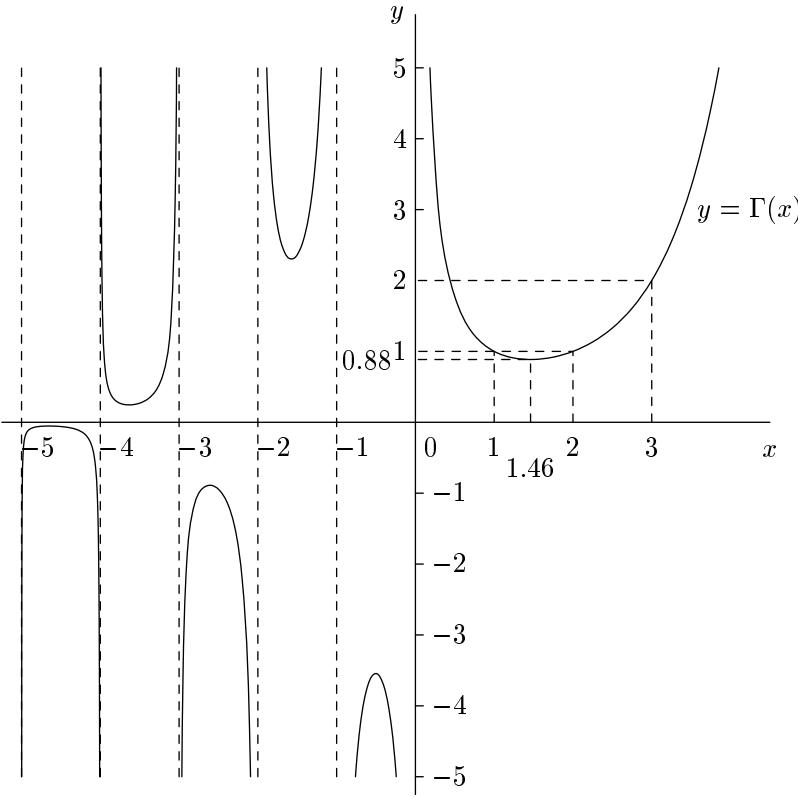
\includegraphics[keepaspectratio]{images/part002_cfbcc1f6.jpg}}\\
图 1\\
因而 \(\Gamma''(x)\) 与 \(\Gamma(x)\) 有相同的符号；于是 \(\Gamma\) 在 x \textgreater{} 0 时以及 \(-(2n + 2) < x < -(2n + 1)\) 时凸，在 \(-(2n + 1) < x - 2n\) 时凹（ \(n \in N\) ）；由此推出，在 \(\Gamma\) 凸的区间上，\(\Gamma'(x)\) 从 \(-\infty\) 递增到 \(+\infty\) ，而在 \(\Gamma\) 凹的区间上，\(\Gamma'(x)\) 从 \(+\infty\) 递减到 \(-\infty\) 。由此得到 \(\Gamma\) 的图像（图 1）。

\subsection{欧拉积分}

为简便起见，我们称一个函数 \(f\) （定义在区间 \(I \subset \mathbf{R}\) 上，且在此区间上 \(> 0\) ）在 \(I\) 上是对数凸的，如果 \(\log f\) 在 \(I\) 上是凸的。\(\Gamma(x)\) 的定义表明这个函数在 \(]0, +\infty[\) 上是对数凸的。

显然，I 上两个对数凸函数的乘积在 I 上也是对数凸的。此外：

引理 1. 设 \(f\) 与 \(g\) 是开区间 I 上两个 \(> 0\) 且两次可导的函数。若 \(f\) 与 \(g\) 都是 I 上的对数凸函数，则 \(f + g\) 在 I 上也是对数凸的。

关系式 \(\mathrm{D}^{2}\left(\log f(x)\right) \geqslant 0\) 可以写成 \(f(x)f''(x) - \left(f'(x)\right)^{2} \geqslant 0\) 。于是只需证明：关系式 a \textgreater{} 0、\(a' > 0\)、\(ac - b^{2} \geqslant 0\)、\(a'c' - b'^{2} \geqslant 0\) 蕴含 \((a + a')(c + c') - (b + b')^{2} \geqslant 0\) ；而当 a \textgreater{} 0 时，关系式 \(ac - b^{2} \geqslant 0\) 等价于二次型 \(ax^{2} + 2bxy + cy^{2}\) 为 \(\geqslant 0\) （在 \(R^{2}\) 上）这一事实，且显然，若

\[
a x ^ {2} + 2 b x y + c y ^ {2} \geqslant 0 \quad \text { and } \quad a ^ {\prime} x ^ {2} + 2 b ^ {\prime} x y + c ^ {\prime} y ^ {2} \geqslant 0
\]

在 \(\mathbf{R}^{2}\) 上成立，则 \((a + a')x^{2} + 2(b + b')xy + (c + c')y^{2} \geqslant 0\) 在 \(\mathbf{R}^{2}\) 上也成立。

引理 2. 设 \(f\) 是一个有限实值函数，\(>0\) ，在积 \(I \times J\) （\(\mathbf{R}\) 中两个开区间之积）上有定义且连续，并使得对每个 \(t \in J\) ，函数 \(x \mapsto f(x,t)\) 在 \(I\) 上是对数凸的且两次可导。在这些假设下，若积分 \(g(x) = \int_{J} f(x,t) dt\) 对每个 \(x \in I\) 收敛，则 \(g\) 在 \(I\) 上是对数凸的。

首先证明，对每个紧区间 \(K \subset J\) ，函数 \(g_{K}(x) = \int_{K} f(x, t) dt\) 是对数凸的。事实上，若 \(K = [a, b]\) ，则函数序列

\[
g _ {n} (x) = \frac {b - a}{n} \sum_ {k = 0} ^ {n - 1} f \left(x, a + k \frac {b - a}{n}\right)
\]

在 I 上简单收敛于 \(g_{K}(x)\) （II, p.~57, prop. 5），因而 \(\log g_{n}\) 简单收敛于 \(\log g_{K}\) ；由 VII, p.~310 的引理 1，\(\log g_{n}\) 在 I 上是凸的，故（I, p.~27, prop. 4）\(\log g_{K}\) 也是凸的。

另一方面，g 是 \(g_{K}\) 沿 I 的紧子区间所成的定向集的逐点极限（II, p.~64），故 \(\log g\) 是诸 \(\log g_{K}\) 的逐点极限；这些函数在 I 上都是凸的，因而 \(\log g\) 也是凸的（I, p.~27, prop. 4）。

容易证明，即使不假设函数两次可导，引理 1 与引理 2 仍然成立（VII, p.~327, exerc. 5）。

引理 3. 设 \(\varphi\) 是一个连续且 \(>0\) 的函数，定义在开区间 \(J\) （含于 \([0, +\infty[\) ）上。若 \(I\) 是使积分 \(g(x) = \int_{J} t^{x-1} \varphi(t) dt\) 对一切 \(x \in I\) 收敛的开区间，则 \(g\) 在 \(I\) 上是对数凸的。

事实上，\(\log t^{x - 1} = (x - 1)\log t\) 作为 \(x\) 的函数，对一切 \(t > 0\) 是凸的且两次可导的，故引理 2 适用。

命题 3. 对一切 \(x > 0\)

\[
\Gamma (x) = \int_ {0} ^ {\infty} e ^ {- t} t ^ {x - 1} d t\tag{14}
\]

（第二类欧拉积分）。

现在，函数 \(g(x) = \int_0^\infty e^{-t} t^{x-1} dt\) 对一切 \(x > 0\) 有定义（V, p.~229）；于是由 VII, p.~311 的引理 3，它在 \(]0, +\infty[\) 上是对数凸的。此外，分部积分给出

\[
g (x + 1) = \int_ {0} ^ {\infty} e ^ {- t} t ^ {x} d t = - e ^ {- t} t ^ {x} \Big | _ {0} ^ {\infty} + x \int_ {0} ^ {\infty} e ^ {- t} t ^ {x - 1} d t = x g (x).
\]

换句话说，g 是 VII, p.~305 的方程 (1) 的一个解；最后，

\[
g (1) = \int_ {0} ^ {\infty} e ^ {- t} d t = 1;
\]

因而命题由 VII, p.~306 的 prop. 1 得出。

由变量替换 \(e^{-t}=u\) ，从 (14) （VII, p.~311）推出公式

\[
\Gamma (x) = \int_ {0} ^ {1} \left(\log \frac {1}{t}\right) ^ {x - 1} d t.\tag{15}
\]

同样，由变量替换 \(u = t^{x}\) 得到

\[
x \Gamma (x) = \int_ {0} ^ {\infty} e ^ {- t ^ {1 / x}} d t
\]

或者再利用 (7) （VII, p.~3），得

\[
\Gamma \left(1 + \frac {1}{x}\right) = \int_ {0} ^ {\infty} e ^ {- t ^ {x}} d t\tag{16}
\]

而特别地，对 \(x = 2\) ，有

\[
\Gamma \left(\frac {3}{2}\right) = \frac {1}{2} \Gamma \left(\frac {1}{2}\right) = \int_ {0} ^ {\infty} e ^ {- t ^ {2}} d t.\tag{17}
\]

命题 4. 对 x \textgreater{} 0 与 y \textgreater{} 0 ，积分

\[
\mathbf {B} (x, y) = \int_ {0} ^ {1} t ^ {x - 1} (1 - y) ^ {y - 1} d t
\]

（第一类欧拉积分）取值

\[
\mathbf {B} (x, y) = \frac {\Gamma (x) \Gamma (y)}{\Gamma (x + y)}.\tag{18}
\]

事实上，这个积分对 \(x > 0\) 与 \(y > 0\) 收敛（V, p.~229）。由 VII, p.~311 的引理 3，函数 \(x \mapsto \mathbf{B}(x, y)\) 对 \(x > 0\) 是对数凸的。此外，

\[
\mathbf {B} (x + 1, y) = \int_ {0} ^ {1} (1 - t) ^ {x + y - 1} \left(\frac {t}{1 - t}\right) ^ {x} d t
\]

于是，由分部积分得

\[
\begin{array}{l} \mathbf {B} (x + 1, y) = - \frac {(1 - t) ^ {x + y}}{x + y} \left(\frac {t}{1 - t}\right) ^ {x} \Bigg | _ {0} ^ {1} \\ \qquad + \frac {x}{x + y} \int_ {0} ^ {1} (1 - t) ^ {x + y} \left(\frac {t}{1 - t}\right) ^ {x - 1} \frac {d t}{(1 - t) ^ {2}} = \frac {x}{x + y} \mathbf {B} (x, y). \end{array}
\]

由此推出，\(f(x) = \mathbf{B}(x, y) \Gamma(x + y)\) 满足 VII, p.~305 的恒等式 (1) 。而且，这个函数作为两个对数凸函数的乘积，是对数凸的。最后，有 \(f(1) = \mathbf{B}(1, y) \Gamma(y + 1)\) ，而 \(\mathbf{B}(1, y) = \int_{0}^{1} (1 - t)^{y - 1} dt = 1/y\) ，故 \(f(1) = \frac{1}{y} \Gamma(y + 1) = \Gamma(y)\) 。于是由 VII, p.~306 的 prop. 1，函数 \(f(x)/\Gamma(y)\) 等于 \(\Gamma(x)\) ，这就证明了 (18)。

由变量替换 \(t = \frac{u}{u + 1}\) ，公式 (18) 变为

\[
\int_ {0} ^ {\infty} \frac {t ^ {x - 1}}{(1 + t) ^ {x + y}} d t = \frac {\Gamma (x) \Gamma (y)}{\Gamma (x + y)}\tag{19}
\]

而由变量替换 \(t = \sin^{2} \varphi\) ，得

\[
\int_ {0} ^ {\pi / 2} \sin^ {2 x - 1} \varphi \cos^ {2 y - 1} \varphi d \varphi = \frac {1}{2} \frac {\Gamma (x) \Gamma (y)}{\Gamma (x + y)}.\tag{20}
\]

在这最后一个公式中取 \(x = y = \frac{1}{2}\) ，便得

\[
\Gamma (\frac {1}{2}) = \sqrt {\pi}\tag{21}
\]

再由 (17) ，得

\[
\int_ {0} ^ {\infty} e ^ {- t ^ {2}} d t = \frac {1}{2} \sqrt {\pi}.\tag{22}
\]

由 VII, p.~307 的关系式 (7) ，有渐近展开

\[
\begin{array}{l} \Gamma (x) = \frac {1}{x} \Gamma (x + 1) \\ = \frac {1}{x} + \Gamma^ {\prime} (1) + \frac {1}{2 !} \Gamma^ {\prime \prime} (1) x + \dots + \frac {1}{n !} \Gamma^ {(n)} (1) x ^ {n - 1} + O (x ^ {n}) \end{array}\tag{23}
\]

这是 \(\Gamma(x)\) 在 0 的一个邻域中的渐近展开。

同样，对每个固定的 y 且 \textgreater{} 0 ，可以写出

\[
\begin{array}{l} \frac {1}{\Gamma (x + y)} = \frac {1}{\Gamma (y)} + D \left(\frac {1}{\Gamma (y)}\right) x \\ \qquad + \frac {1}{2 !} D ^ {2} \left(\frac {1}{\Gamma (y)}\right) x ^ {2} + \dots + \frac {1}{n !} D ^ {n} \left(\frac {1}{\Gamma (y)}\right) x ^ {n} + O _ {1} (x ^ {n + 1}) \end{array}
\]

于是公式 (18) 给出，对固定的 y ，渐近展开

\[
\begin{array}{l} \mathbf {B} (x, y) = \frac {1}{x} + \left(\Gamma^ {\prime} (1) - \frac {\Gamma^ {\prime} (y)}{\Gamma (y)}\right) \\ \qquad + \left(\frac {\Gamma^ {\prime \prime} (1)}{2} - \Gamma^ {\prime} (1) \frac {\Gamma^ {\prime} (y)}{\Gamma (y)} + \frac {2 \Gamma^ {\prime 2} (y) - \Gamma (y) \Gamma^ {\prime \prime} (y)}{2 \Gamma^ {2} (y)}\right) x + O (x ^ {2}) \end{array}\tag{24}
\]

在 \(x = 0\) 的一个邻域中成立。

此外，对 x \textgreater{} 0 与 y \textgreater{} 0 ，有

\[
\begin{array}{l} \mathbf {B} (x, y) = \int_ {0} ^ {1} \left(t ^ {x - 1} + t ^ {x} \frac {(1 - t) ^ {y - 1} - 1}{t}\right) d t \\ = \frac {1}{x} + \int_ {0} ^ {1} t ^ {x} \frac {(1 - t) ^ {y - 1} - 1}{t} d t. \end{array}\tag{25}
\]

函数 \(\varphi(t) = \frac{(1 - t)^{y - 1} - 1}{t}\) 在紧区间 {[}0, 1{]} 上连续；由于

\[
t ^ {x} = e ^ {x \log t} = 1 + x \log t + \frac {x ^ {2}}{2 !} (\log t) ^ {2} + \dots + \frac {x ^ {n}}{n !} (\log t) ^ {n} + r _ {n} (x, t)
\]

其中 \(|r_n(x,t)| \leqslant \frac{x^{n+1}}{(n+1)!} |\log t|^{n+1}\) （因为 \(\log t \leqslant 0\) 且 \(x > 0\) ），公式 (25) 给出渐近展开

\[
\begin{array}{l} \mathbf {B} (x, y) = \frac {1}{x} + \int_ {0} ^ {1} \varphi (t) d t + x \int_ {0} ^ {1} \varphi (t) \log t d t + \dots \\ \qquad + \frac {x ^ {n}}{n !} \int_ {0} ^ {1} \varphi (t) (\log t) ^ {n} d t + O _ {2} (x ^ {n + 1}) \end{array}
\]

这是 \(\mathbf{B}(x,y)\) 在 0 的一个邻域中的渐近展开。

对 \(n = 1\) ，把这一展开与 (24) 等同起来，特别得到

\[
\Gamma^ {\prime} (1) - \frac {\Gamma^ {\prime} (y)}{\Gamma (y)} = \int_ {0} ^ {1} \frac {(1 - t) ^ {y - 1} - 1}{t} d t.
\]

此外，公式 (10) 给出 \(\Gamma'(1) = \Gamma'(1)/\Gamma(1) = -\gamma\) ，于是（高斯积分）

\[
\frac {\Gamma^ {\prime} (x)}{\Gamma (x)} + \gamma = \int_ {0} ^ {1} \frac {1 - (1 - t) ^ {x - 1}}{t} d t.\tag{26}
\]

\section{复数域中的 Γ 函数}

\subsection{Γ 函数到 C 上的延拓}

我们回到魏尔斯特拉斯公式，它给出表达式

\[
\frac {1}{\Gamma (x)} = x e ^ {\gamma x} \prod_ {n = 1} ^ {\infty} \left(1 + \frac {x}{n}\right) e ^ {- x / n}\tag{1}
\]

\(1 / \Gamma (x)\) （对一切实数 \(x\) ）；现考虑以 \(\left(1 + \frac{z}{n}\right)e^{-z / n}\) 为通项、以任意复数 \(z\) 为变量的无穷乘积。可以写 \(e^{-z / n} = 1 - \frac{z}{n} + h(z)\) ，其中 \(|h(z)| \leqslant \frac{|z|^2}{2n^2} e^{|z / n|}\) （III, p.~106, 公式 (8)），于是

\[
\left(1 + \frac {z}{n}\right) e ^ {- z / n} = 1 + v _ {n} (z)
\]

其中 \(|v_{n}(z)| \leqslant \frac{|z|^{2}}{n^{2}}\left(1 + \frac{e^{|z|}}{2}(1 + |z|)\right)\) ；因此所考虑的无穷乘积在 C 的每个紧子集上绝对且一致收敛；而且，它的值仅在点 z = -n 处为零（Gen.~Top., IX, p.~214, corollary）。鉴于 VII, p.~315 的公式 (1) ，对每个复数 z ，令

\[
\frac {1}{\Gamma (z)} = z e ^ {\gamma z} \prod_ {n = 1} ^ {\infty} \left(1 + \frac {z}{n}\right) e ^ {- z / n}.\tag{2}
\]

这样，函数 \(\Gamma(z)\) 对每个点 \(z \in \mathbf{C}\) （除点 \(-n\) （ \(n \in \mathbf{N}\) ）以外）都有定义；它在这个集合上连续，并且 \((z + n)\Gamma(z) \sim \frac{(-1)^n}{n!}\) （在 \(-n\) 的一个邻域中）。公式 (2) 表明，有 \(\Gamma(\overline{z}) = \overline{\Gamma(z)}\) （对每个异于负整数的 \(z\) ）。

从高斯公式（VII, p.~307, 公式 (8)）过渡到魏尔斯特拉斯公式的论证，将其中的步骤倒转，也适用于复数 \(z\) ，并且表明，对 \(z \neq -n\) （ \(n \in \mathbf{N}\) ），有

\[
\Gamma (z) = \lim _ {n \rightarrow \infty} \frac {n ^ {z} n !}{z (z + 1) \dots (z + n)}\tag{3}
\]

这里约定取 \(n^z = e^{z\log n}\) 。由于

\[
\frac {n ^ {z + 1} n !}{(z + 1) (z + 2) \dots (z + n + 1)} = z \frac {n}{n + 1 + z} \frac {n ^ {z} n !}{z (z + 1) \dots (z + n)}
\]

取极限，再次得到基本泛函方程

\[
\Gamma (z + 1) = z \Gamma (z)\tag{4}
\]

对每个 \(z \neq -n (n \in \mathbf{N})\) 成立。

设 \(p\) 是任意整数 \(> 0\) ，\(\mathrm{K}_p\) 为开圆盘 \(|z| < p\) ；对每个 \(z \in \mathrm{K}_p\) 与每个整数 \(n > p\) ，\(1 + \frac{z}{n}\) 不是负实数，故 \(\log \left(1 + \frac{z}{n}\right)\) 有定义，且由上所述，以 \(\log \left(1 + \frac{z}{n}\right) - \frac{z}{n} (n > p)\) 为通项的级数在 \(\mathrm{K}_p\) 上正规收敛；对通项微分有限次所得的级数也同样如此，因为有

\[
\left| \frac {1}{n} - \frac {1}{z + n} \right| \leqslant \frac {p}{n (n - p)} \quad \text { and } \quad \left| \frac {1}{(z + n) ^ {k}} \right| \leqslant \frac {1}{(n - p) ^ {k}} \quad (k > 1)
\]

对 \(z \in \mathbf{K}_p\) 与 \(n > p\) 成立。于是可以看出（cf.~II, p.~59, 注 3），\(\Gamma(z)\) 在所有点 \(z \in \mathbf{C}\) （除诸点 \(-n\) 以外）处无穷次可导，且在这些点处有

\[
{\frac {\Gamma^ {\prime} (z)}{\Gamma (z)}} = - \gamma - {\frac {1}{z}} + \sum_ {n = 1} ^ {\infty} \left({\frac {1}{n}} - {\frac {1}{z + n}}\right)\tag{5}
\]

\[
\mathrm{D} ^ {k - 1} \left(\frac {\Gamma^ {\prime} (z)}{\Gamma (z)}\right) = \sum_ {n = 0} ^ {\infty} \frac {(- 1) ^ {k} (k - 1) !}{(z + n) ^ {k}} \quad \text { for } \quad k \geqslant 2,\tag{6}
\]

其中 (5) 与 (6) 的右端在 \(\mathbf{C}\) 的每个不含任何整数 \(\leqslant 0\) 的紧子集上正规收敛。此外，可以写

\[
\log \Gamma (z) \equiv - \gamma z - \log z + \sum_ {n = 1} ^ {\infty} \left(\frac {z}{n} - \log \left(1 + \frac {z}{n}\right)\right) \pmod {2 \pi i}\tag{7}
\]

这里约定：当此公式中的某个对数是负实数的对数时，就在该点处取相差 \(2\pi i\) 的 \(\log z\) 的这一个或那一个极限值；于是 (7) 右端的级数在 C 的每个不含任何整数 \(\leqslant 0\) 的紧子集上正规收敛。

\subsection{余元公式与勒让德–高斯倍乘公式}

由 VII, p.~315 的公式 (2) 立即导出，对每个 \(z \in C\) ，

\[
\frac {1}{\Gamma (z) \Gamma (- z)} = - z ^ {2} \prod_ {n = 1} ^ {\infty} \left(1 - \frac {z ^ {2}}{n ^ {2}}\right).
\]

而 \(\sin z\) 的欧拉展开（VI, p.~287, th. 2）表明

\[
z \prod_ {n = 1} ^ {\infty} \left(1 - \frac {z ^ {2}}{n ^ {2}}\right) = \frac {1}{\pi} \sin \pi z;
\]

再利用 VII, p.~315 的泛函方程 (4) ，便得到：

命题 1. 对每个复数 \(z\) ，有

\[
\frac {1}{\Gamma (z) \Gamma (1 - z)} = \frac {1}{\pi} \sin \pi z\tag{8}
\]

（余元公式）。

推论 --- 对每个实数 t ，有

\[
| \Gamma (i t) | = \sqrt {\frac {\pi}{t \sinh \pi t}} \qquad (t \neq 0)\tag{9}
\]

\[
\left| \Gamma (\frac {1}{2} + i t) \right| = \sqrt {\frac {\pi}{\cosh \pi t}}.\tag{10}
\]

事实上，由 (8) 推出 \(\Gamma(it)\Gamma(-it) = \frac{i\pi}{t\sin\pi it} = \frac{\pi}{t\sinh\pi t}\) ，且有 \(\Gamma(-it) = \overline{\Gamma(it)}\) ；同样，(8) 给出

\[
\Gamma \left(\frac {1}{2} + i t\right) \Gamma \left(\frac {1}{2} - i t\right) = \frac {\pi}{\sin \left(\frac {\pi}{2} + \pi i t\right)} = \frac {\pi}{\cos \pi i t} = \frac {\pi}{\cosh \pi t},
\]

并且有

\[
\Gamma \bigl (\frac {1}{2} - i t \bigr) = \overline {{\Gamma \bigl (\frac {1}{2} + i t \bigr)}}.
\]

现设 \(p\) 是任意整数 \(> 0\) ，考虑乘积

\[
f (z) = \Gamma \left(\frac {z + 1}{p}\right) \Gamma \left(\frac {z + 2}{p}\right) \dots \Gamma \left(\frac {z + p}{p}\right).
\]

由 (3) （VII, p.~315），对每个 \(z \neq -n\) （ \(n \in \mathbf{N}\) ），\(f(z)\) 是乘积

\[
\begin{array}{c} \frac {n ^ {(z + 1) / p} n !}{\left(\frac {z + 1}{p}\right) \left(\frac {z + 1}{p} + 1\right) \cdots \left(\frac {z + 1}{p} + n\right)}. \\ \frac {n ^ {(z + 2) / p} n !}{\left(\frac {z + 2}{p}\right) \left(\frac {z + 2}{p} + 1\right) \cdots \left(\frac {z + 2}{p} + n\right)} \dots \\ \dots \frac {n ^ {(z + p) / p} n !}{\left(\frac {z + p}{p}\right) \left(\frac {z + p}{p} + 1\right) \cdots \left(\frac {z + p}{p} + n\right)} \\ = \frac {n ^ {z + (p + 1) / 2} p ^ {(n + 1) p} (n !) ^ {p}}{(z + 1) (z + 2) \ldots (z + (n + 1) p)} \end{array}
\]

的极限；特别地，\(f(0)\) 是乘积

\[
\frac {n ^ {(p + 1) / 2} p ^ {(n + 1) p} (n !) ^ {p}}{((n + 1) p) !}
\]

由此推出，\(f(z) / f(0)\) 是

\[
\begin{array}{c} \frac {n ^ {z} ((n + 1) p) !}{(z + 1) (z + 2) \dots (z + (n + 1) p)} \\ = z   p ^ {- z} \left(\frac {n}{n + 1}\right) ^ {z}. \frac {((n + 1) p) ^ {z} ((n + 1) p) !}{z (z + 1) (z + 2) \dots (z + (n + 1) p)} \end{array}
\]

的极限；于是由 (3) （VII, p.~315）得

\[
f (z) = f (0) z p ^ {- z} \Gamma (z).\tag{11}
\]

但是，可以写

\[
f (0) = \prod_ {k = 1} ^ {p - 1} \Gamma \left(\frac {k}{p}\right) = \prod_ {k = 1} ^ {p - 1} \Gamma \left(1 - \frac {k}{p}\right) = \sqrt {\prod_ {k = 1} ^ {p - 1} \Gamma \left(\frac {k}{p}\right) \Gamma \left(1 - \frac {k}{p}\right)}
\]

由于 \(f(0) > 0\) ；于是余元公式给出

\[
f (0) = \sqrt {\pi^ {p - 1} / \prod_ {k = 1} ^ {p - 1} \sin \frac {k \pi}{p}}
\]

又由于右端的乘积等于 \(p/2^{p-1}\) （VI, p.~284, cor. 1），最终得到：

命题 2. 对每个不是整数 \(\leqslant 0\) 的复数 z 以及每个整数 p \textgreater{} 0 ，有

\[
\Gamma \left(\frac {z}{p}\right) \Gamma \left(\frac {z + 1}{p}\right) \dots \Gamma \left(\frac {z + p - 1}{p}\right) = (2 \pi) ^ {(p - 1) / 2} p ^ {\frac {1}{2} - z} \Gamma (z)\tag{12}
\]

（勒让德–高斯倍乘公式）。

命题 3. 对每个实数 x \textgreater{} 0 ，有

\[
\int_ {x} ^ {x + 1} \log \Gamma (t) d t = x (\log x - 1) + \frac {1}{2} \log 2 \pi\tag{13}
\]

（拉阿贝积分）。

首先对 \(x = 0\) 证明公式 (13) 。由于 \(\log \Gamma(x) \sim \log \frac{1}{x}\) （当 \(x\) 趋于 0 时），积分 \(\int_0^1 \log \Gamma(x) dx\) 收敛。此外，函数 \(\log \Gamma(x)\) 在 {[}0, 1{]} 上递减（VII, p.~310）；于是对每个 \(\alpha > 0\) 有

\[
\frac {1}{n} \sum_ {k = 1} ^ {q} \log \Gamma \left(\frac {k}{n}\right) \leqslant \int_ {0} ^ {\alpha} \log \Gamma (x) d x,
\]

其中 \(q\) 是使 \(q / n \leqslant \alpha\) 的最大整数。由于 \(\int_{0}^{\alpha} \log \Gamma(x) dx\) 随 \(\alpha\) 而趋于 0 ，且 \(\frac{1}{n} \sum_{k=q+1}^{n} \log \Gamma\left(\frac{k}{n}\right)\) 趋于 \(\int_{\alpha}^{1} \log \Gamma(x) dx\) （当 \(n\) 趋于 \(+\infty\) 时；II, p.~57, prop. 5） ，故有

\[
\int_ {0} ^ {1} \log \Gamma (x) d x = \lim _ {n \rightarrow \infty} \frac {1}{n} \sum_ {k = 1} ^ {n} \log \Gamma \left(\frac {k}{n}\right).
\]

而由 (12) ，此公式右端是

\[
\frac {n - 1}{2 n} \log 2 \pi - \frac {1}{2} \frac {\log n}{n},
\]

的极限，由此得

\[
\int_ {0} ^ {1} \log \Gamma (x) d x = \frac {1}{2} \log 2 \pi .\tag{14}
\]

其次我们注意到，由恒等式

\[
\log \Gamma (x + 1) = \log \Gamma (x) + \log x
\]

积分后得到，对 x \textgreater{} 0

\[
\int_ {0} ^ {x} \log \Gamma (t + 1) d t = \int_ {0} ^ {x} \log \Gamma (t) d t + \int_ {0} ^ {x} \log t d t.
\]

但左端的积分也等于 \(\int_{1}^{x + 1}\log \Gamma (t)dt\) 。于是由 (14) ，

\[
\int_ {x} ^ {x + 1} \log \Gamma (t) d t = \int_ {0} ^ {x} \log t d t + \frac {1}{2} \log 2 \pi = x (\log x - 1) + \frac {1}{2} \log 2 \pi .
\]

\subsection{斯特林展开}

设 \(x\) 与 \(y\) 是两个不在实负半轴上的复数；由 VII, p.~315 的公式 (3) ，并依照 VII, p.~316 关于对数的约定，\(\log \Gamma(x) - \log \Gamma(y)\) 模 \(2\pi i\) 同余于表达式

\[
(x - y) \log n + \sum_ {k = 0} ^ {n} \Big (\log (y + k) - \log (x + k) \Big).\tag{15}
\]

令 \(f(t) = \log(y + t) - \log(x + t)\) ；对函数 f 应用欧拉–麦克劳林求和公式（VI, p.~288）：

\[
\begin{array}{l} f (0) + f (1) + \dots + f (n) = \int_ {0} ^ {n + 1} f (t) d t - \frac {1}{2} \big (f (n + 1) - f (0) \big) \\ \qquad + \sum_ {k = 1} ^ {p} \frac {b _ {2 k}}{(2 k) !} \big (f ^ {(2 k - 1)} (n + 1) - f ^ {(2 k - 1)} (0) \big) + T _ {p} (n) \end{array}
\]

其中

\[
\left| \mathrm{T} _ {p} (n) \right| \leqslant \frac {4 e ^ {2 \pi}}{(2 \pi) ^ {2 p + 1}} \int_ {0} ^ {n + 1} \left| f ^ {(2 p + 1)} (u) \right| d u.\tag{16}
\]

由于

\[
f ^ {(m)} (t) = (- 1) ^ {m - 1} (m - 1)! \left(\frac {1}{(y + t) ^ {m}} - \frac {1}{(x + t) ^ {m}}\right),
\]

\(f^{(2k - 1)}(n + 1)\) 当 \(n\) 趋于 \(+\infty\) 时趋于 0 （对一切 \(k \geqslant 1\) ）；对

\[
f (n + 1) = \log \left(1 + \frac {y}{n + 1}\right) - \log \left(1 + \frac {x}{n + 1}\right).
\]

此外，有

\[
\int_ {0} ^ {n + 1} \log (x + t) d t = (x + n + 1) (\log (x + n + 1) - 1) - x (\log x - 1);
\]

当 n 趋于 \(+\infty\) 时，有渐近展开

\[
(x + n) \bigl (\log (x + n) - 1 \bigr) = n \log n - n + x \log n + O \left(\frac {1}{n}\right).
\]

把这些结果代入表达式 (15) ，最终可以看出，当 n 趋于 \(+\infty\) 时，\(\mathrm{T}_{p}(n)\) 有极限 \(\mathrm{R}_{p}(x, y)\) ，并且可以写

\[
\log \Gamma (x) - g (x) \equiv \log \Gamma (y) - g (y) + \mathrm{R} _ {p} (x, y)\tag{mod.  \( 2\pi i \)}
\]

其中令

\[
g (x) = x \log x - x - \frac {1}{2} \log x + \sum_ {k = 1} ^ {p} \frac {b _ {2 k}}{2 k (2 k - 1)} \frac {1}{x ^ {2 k - 1}}.\tag{17}
\]

现在我们借助 (16) 来估计 \(\mathrm{R}_{p}(x,y)\) 的一个上界，假设 x 与 y 都属于 C 中的子集 \(H_{A}\) ——由关系式`` \(\mathcal{R}(z)\geqslant A\) 或 \(|\mathcal{I}(z)|\geqslant A\) ''所定义——其中 A 是任意数 \textgreater0 （图~2）。为此我们注意到，若 \(x=s+it\) 且 s\textgreater A ，则有 \(|x+u|\geqslant A+u\) （对每个 u\textgreater0 ），因而

\[
\int_ {0} ^ {n + 1} \frac {d u}{| x + u | ^ {2 p + 1}} \leqslant \int_ {0} ^ {\infty} \frac {d u}{(\mathrm{A} + u) ^ {2 p + 1}} = \frac {1}{2 p \mathrm{A} ^ {2 p}}.
\]

同样，若 \(|t| \geqslant A\) ，则有 \(|x + u| = |s + u + it| \geqslant \sqrt{A^2 + (s + u)^2}\) （对一切实数 \(u\) ），由此得

\[
\int_ {0} ^ {n + 1} \frac {d u}{| x + u | ^ {2 p + 1}} \leqslant \int_ {- \infty} ^ {+ \infty} \frac {d u}{(\mathrm{A} ^ {2} + u ^ {2}) ^ {p + 1 / 2}} = \frac {2}{\mathrm{A} ^ {2 p}} \int_ {0} ^ {\infty} \frac {d v}{(1 + v ^ {2}) ^ {p + 1 / 2}}.
\]

于是可以看出，当 x 与 y 属于 \(H_{A}\) 时，有

\[
\left| \mathrm{R} _ {p} (x, y) \right| \leqslant \frac {\mathrm{C} _ {p}}{\mathrm{A} ^ {2 p}}
\]

\pandocbounded{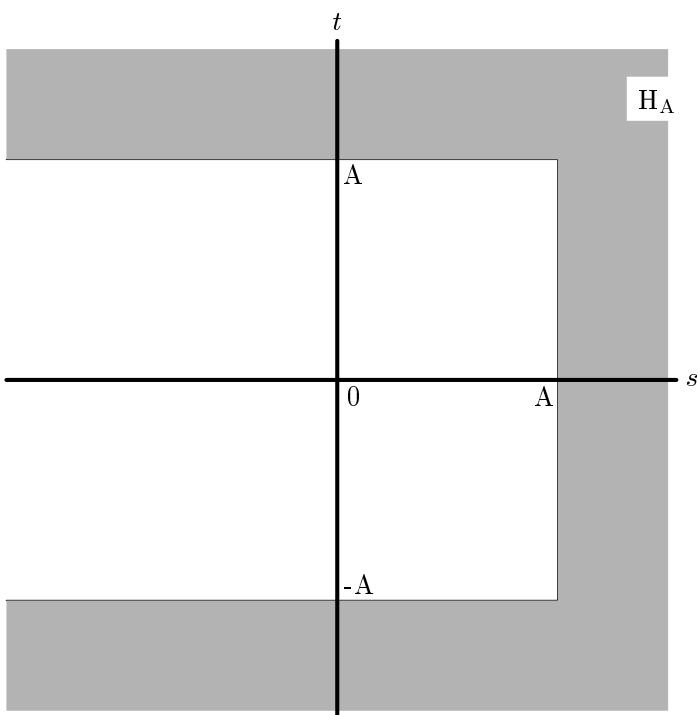
\includegraphics[keepaspectratio]{images/part002_194eed20.jpg}}\\
图 2

其中 \(C_{p}\) 仅依赖于 p。现设 F 是以诸集 \(H_{A}\) 为基的滤子；柯西准则表明，沿滤子 F ，函数 \(\log \Gamma(z) - g(z)\) 有一个有限极限 \(\delta\) （模 \(2\pi i\) ） ，并且，若令 \(\omega(z) = \max(\mathcal{R}(z), |\mathcal{I}(z)|)\) ，则有

\[
\log \Gamma (z) - g (z) - \delta \equiv O \left(\frac {1}{(\omega (z)) ^ {2 p}}\right) \pmod {2 \pi i}.\tag{18}
\]

对实数 \(x\) 且 \(> 0\) ，有 \(\Gamma(x) > 0\) ，且 \(g(x)\) 是实数，故可以设 \(\delta\) 是实数，并有

\[
\log \Gamma (x) = g (x) + \delta + O \left(\frac {1}{x ^ {2 p}}\right).
\]

现在来确定常数 \(\delta\) 的值；把 VII, p.~318 的 prop. 2 应用于 p = 2 ，则当实数 x 趋于 \(+\infty\) 时，有

\[
\begin{array}{c} \frac {x - 1}{2} \log \frac {x}{2} - \frac {x}{2} + \frac {x}{2} \log \frac {x + 1}{2} - \frac {x + 1}{2} + 2 \delta \\ = x \log x - x - \frac {1}{2} \log x + (\frac {1}{2} - x) \log 2 + \frac {1}{2} \log 2 \pi + \delta + o (1) \end{array}
\]

由此容易推出 \(\delta = \frac{1}{2}\log 2\pi\) 。最后有下列结果：

命题 4. 沿滤子 \(\mathfrak{F}\) ，有（对每个整数 \(p \geqslant 1\) ）渐近展开

\[
\begin{array}{l} \log \Gamma (z) \equiv z \log z - z - \frac {1}{2} \log z + \frac {1}{2} \log 2 \pi \\ \quad + \sum_ {k = 1} ^ {p} \frac {b _ {2 k}}{2 k (2 k - 1)} \frac {1}{z ^ {2 k - 1}} + O \left(\frac {1}{(\omega (z)) ^ {2 p}}\right) \pmod {2 \pi i} \end{array}\tag{19}
\]

（斯特林展开）。

推论. 沿滤子 F ，有

\[
\Gamma (z) \sim \sqrt {2 \pi} \exp (z \log z - z - \frac {1}{2} \log z).\tag{20}
\]

特别地，当实数 \(x\) 趋于 \(+\infty\) 时，公式 (20) 可以写成

\[
\Gamma (x) \sim \sqrt {2 \pi} x ^ {x - 1 / 2} e ^ {- x},\tag{21}
\]

于是，当整数 n 趋于 \(+\infty\) 时，

\[
n! \sim \sqrt {2 \pi} n ^ {n + 1 / 2} e ^ {- n}
\]

（cf.~V, p.~244）。

由此可以导出许多公式。例如，对每个复数 \(\alpha\) 与每个整数 n ，当 n 趋于 \(+\infty\) 时，有

\[
\frac {\Gamma (n + \alpha)}{\Gamma (n)} \sim n ^ {\alpha} \quad (= e ^ {\alpha \log n}).\tag{22}
\]

同样，对每个不是整数 \(\leqslant 0\) 的复数 a ，有

\[
a (a + 1) (a + 2) \dots (a + n) = \frac {\Gamma (n + a + 1)}{\Gamma (a)} \sim \frac {\sqrt {2 \pi}}{\Gamma (a)} n ^ {n + a + 1 / 2} e ^ {- n}\tag{23}
\]

而对每个不是整数 \(\geqslant 0\) 的复数 a ，有

\[
\binom {a} {n} = \frac {(- 1) ^ {n}}{\Gamma (- a)}   \frac {\Gamma (n - a)}{\Gamma (n + 1)} \sim \frac {(- 1) ^ {n}}{\Gamma (- a)}   n ^ {- a - 1}.\tag{24}
\]

最后，对每个实常数 \(k > 1\) ，有

\[
\binom {k n} {n} = \frac {\Gamma (k n + 1)}{\Gamma (n + 1)   \Gamma ((k - 1) n + 1)} \sim \sqrt {\frac {k}{2 \pi (k - 1) n}} \left(\frac {k ^ {k}}{(k - 1) ^ {k - 1}}\right) ^ {n}.\tag{25}
\]

同样的论证导出下面类似的命题：

命题 5. 沿滤子 \(\mathfrak{F}\) ，有（对每个整数 \(p \geqslant 1\) ）渐近展开

\[
\frac {\Gamma^ {\prime} (z)}{\Gamma (z)} = \log z - \frac {1}{2 z} - \sum_ {k = 1} ^ {p} \frac {b _ {2 k}}{2 k} \frac {1}{z ^ {2 k}} + O \left(\frac {1}{(\omega (z)) ^ {2 p + 1}}\right).\tag{26}
\]

这里不用 VII, p.~318 的 prop. 2 ，而使用公式

\[
\int_ {x} ^ {x + 1} \frac {\Gamma^ {\prime} (t)}{\Gamma (t)} d t = \log \Gamma (x + 1) - \log \Gamma (x) = \log x
\]

来确定常数。

\setcounter{exercisegroup}{0}
\refstepcounter{exercisegroup}
\section*{第 \S\arabic{exercisegroup} 节习题}
\phantomsection
\addcontentsline{toc}{section}{第 \protect\S\arabic{exercisegroup} 节习题}

J 1) 设 \(g\) 是一个规则函数，且 \(>0\) （在 \(]0, +\infty[\) 上）。

\begin{enumerate}
\def\labelenumi{\alph{enumi})}
\tightlist
\item
  设 \(u, v\) 是 \(]0, +\infty[\) 上的两个递增函数，使得 \(u(x + 1) - u(x) = v(x + 1) - v(x) = g(x)\) （对一切 \(x > 0\) ）。证明：若 \(w = u - v\) ，则
\end{enumerate}

\[
\sup _ {0 <   x \leqslant y \leqslant 1} | w (y) - w (x) | \leqslant \inf _ {x > 0} g (x).
\]

（注意，对 \(a \leqslant x \leqslant y \leqslant a + 1\) 有 \(u(y) - u(x) \leqslant g(a)\) 。）特别地，若 \(\inf_{x > 0} g(x) = 0\) ，则在一点处取给定值的方程 \(u(x + 1) - u(x) = g(x)\) 的递增解至多只有一个。

\begin{enumerate}
\def\labelenumi{\alph{enumi})}
\setcounter{enumi}{1}
\tightlist
\item
  设 g 在 {]}0, +∞{[} 上递减。证明级数
\end{enumerate}

\[
\varphi (x) = - g (x) + \sum_ {n = 1} ^ {\infty} (g (n) - g (x + n))
\]

在含于 {]}0, +∞{[} 的每个紧区间上绝对且一致收敛；若 \(\lambda = \lim_{x \to +\infty} g(x)\) ，则函数 \(u(x) = \varphi(x) + \lambda x\) 是方程 \(u(x+1) - u(x) = g(x)\) 的一个递增解。证明：对这个方程的每个递增解 v ，有 \(v(y) - v(x) \geqslant \varphi(y) - \varphi(x)\) （对 0 \textless{} x \textless{} y）。在一点处取给定值的方程 \(u(x+1) - u(x) = g(x)\) 的递增解所成的集，其上（相应地，下）包络是什么？证明这个集仅由一个元素组成当且仅当 \(\lambda = 0\) 。c) 证明：若 \(g(x)\) 递增且 \textgreater0 （在 {[}0, +∞{]} 上），则在一点处取给定值的方程 \(u(x+1) - u(x) = g(x)\) 有无穷多个递增解。d) 设 \(\psi(x)\) 是在 {]}0, +∞{[} 上由下列条件定义的函数：\(\psi(x)=0\) （对 \(0\leqslant x<1\) ）；\(\psi(x)=1\) （对 \(1\leqslant x<2\) ）；\(\psi(x)=n\) （对 \(n-1+\frac{1}{n-1}\leqslant x<n+\frac{1}{n}\) ， \(n\geqslant2\) ）；令 \(g(x)=\psi(x+1)-\psi(x)\) 。证明 \(\psi\) 是方程

\[
u (x + 1) - u (x) = g (x)
\]

使得 \(u(1)=1\) 的唯一递增解。

J2) 设 g 是 {]}0, +∞{[} 上的连续递增函数。

\begin{enumerate}
\def\labelenumi{\alph{enumi})}
\item
  证明：若 \(\liminf_{x\to +\infty}g(x) / x = 0\) ，则在一点处取给定值的方程 \(u(x + 1) - u(x) = g(x)\) 的凸解至多只有一个（注意，对一切 \(h > 0\) ，函数 \(v(x) = u(x + h) - u(x)\) 是满足方程 \(v(x + 1) - v(x) = g(x + h) - g(x)\) 的递增函数，并应用 exerc. 1 a））。
\item
  证明：若 g 在 \(]0, +\infty[\) 上是凹的，则方程 \(u(x+1) - u(x) = g(x)\) 存在凸解；这个方程在一点处取给定值的凸解存在且唯一，当且仅当 \(\lim_{x \to +\infty} g(x)/x = 0\) （cf.~exerc. 1 b））。
\item
  以下设 \(g\) 在 \(]0, +\infty[\) 上递增且凹，并且 \(\lim_{x \to +\infty} g(x) / x = 0\) 。对每对数 \(h > 0\) 、\(k > 0\) 以及每个有限实值函数 \(f\) （定义在 \(]0, +\infty[\) 上），令
\end{enumerate}

\[
\varDelta \Big (f (x); h, k \Big) = \frac {f (x + h) - f (x)}{h} - \frac {f (x) - f (x - k)}{k}
\]

对 x \textgreater{} k。证明：若 u 是方程 \(u(x + 1) - u(x) = g(x)\) 的一个凸解，则有 \(\lim_{x \to +\infty} \Delta(u(x); h, k) = 0\) （对一切 h \textgreater{} 0 与 k \textgreater{} 0）（利用 VII, p.~325 的 exerc. 1 b) 中 \(u_{r}^{\prime}\) 的表达式）。

\(d\) ）用 \(c\) ）的记号证明：存在常数 \(\alpha\) ，使得 \(u(x) = v(x) + \alpha\) ，其中

\[
v (x) = \int_ {1} ^ {x} g (t) d t - \frac {1}{2} g (x) + R (x)
\]

这里令

\[
\mathrm{R} (x) = \sum_ {n = 0} ^ {\infty} h (x + n), \quad h (x) = \int_ {x} ^ {x + 1} g (t) d t - \frac {1}{2} (g (x + 1) + g (x));
\]

并且有

\[
0 \leqslant \mathrm{R} (x) \leqslant \frac {1}{2} (g (x + \frac {1}{2}) - g (x)).
\]

（注意 \(v(x + 1) - v(x) = g(x)\) ，且 \(\lim_{x\to +\infty}\Delta (v(x);h,k) = 0\) （不论 \(h > 0\) 与 \(k > 0\) 如何）。）

\begin{enumerate}
\def\labelenumi{\arabic{enumi})}
\setcounter{enumi}{2}
\tightlist
\item
  \begin{enumerate}
  \def\labelenumii{\alph{enumii})}
  \tightlist
  \item
    设 g 是一个具有连续 \(k^{th}\) 导数的函数，定义在 {]}0, +∞{[} 上，\(g^{(k)}\) 在此区间上递减且 \(\lim_{x\to+\infty}g^{(k)}(x)=0\) 。证明：方程 \(u(x+1)-u(x)=g(x)\) 存在唯一的解 u ，它具有递增的 \(k^{th}\) 导数（在 {]}0, +∞{[} 上）且在一点取给定值（利用 exerc. 1 b)）。
  \end{enumerate}
\end{enumerate}

\begin{enumerate}
\def\labelenumi{\alph{enumi})}
\setcounter{enumi}{1}
\tightlist
\item
  设 \(\alpha\) 是任意实数。设 \(S_{\alpha}\) 是定义在 \(]0, +\infty[\) 上、满足关系式
\end{enumerate}

\[
\mathrm{S} _ {\alpha} (x + 1) - \mathrm{S} _ {\alpha} (x) = x ^ {\alpha}
\]

使 \(S_{\alpha}(1) = 0\) ，此外，\(S_{\alpha}\) 的以 \((\alpha + 1)^{+}\) 的整数部分为阶的导数是递增的（由 \(a\) )，它是唯一的函数）。证明

\[
\mathrm{S} _ {\alpha} ^ {\prime} (x) - \mathrm{S} _ {\alpha} ^ {\prime} (1) = \alpha \mathrm{S} _ {\alpha - 1} (x),
\]

以及

\[
\mathrm{S} _ {\alpha} \left(\frac {x}{p}\right) + \mathrm{S} _ {\alpha} \left(\frac {x + 1}{p}\right) + \dots + \mathrm{S} _ {\alpha} \left(\frac {x + p - 1}{p}\right) = \frac {1}{p ^ {\alpha}} \mathrm{S} _ {\alpha} (x) + \mathrm{C} _ {\alpha}
\]

对每个整数 \(p \geqslant 1\) 成立，其中 \(C_{\alpha}\) 是常数，当 \(\alpha \neq -1\) 时它等于

\[
\left(\frac {1}{p ^ {\alpha}} - p\right) \frac {S _ {\alpha + 1} ^ {\prime} (1)}{\alpha + 1}
\]

（cf.~VII, p.318, prop. 2 与 VI, p.~291, exerc. 3）。

\begin{enumerate}
\def\labelenumi{\arabic{enumi})}
\setcounter{enumi}{3}
\tightlist
\item
  证明函数 \(f(x) = \frac{1}{\sqrt{2}}\frac{\Gamma(x / 2)}{\Gamma\left(\frac{x + 1}{2}\right)}\) 是方程
\end{enumerate}

\(u(x + 1) = 1 / x \, u(x)\) 的唯一凸解（注意此方程蕴含 \(u(x + 2) = \frac{x}{x + 1} \, u(x)\) ，并应用 exerc. 1 a））。

\begin{enumerate}
\def\labelenumi{\arabic{enumi})}
\setcounter{enumi}{4}
\item
  把 VII, p.~310 与 311 的引理 1 与引理 2 推广到任意的对数凸函数（cf.~I, p.~45, exerc. 2）。证明每个对数凸函数都是凸的。
\item
  设 \(\psi(x) = \Gamma'(x)/\Gamma(x)\) ；对每个整数 \(q > 1\) 与每个整数 \(k\) （使 \(1 \leqslant k \leqslant q - 1\) ），建立公式
\end{enumerate}

\[
\sum_ {p = 1} ^ {q} \psi \left(\frac {p}{q}\right) \exp \left(\frac {2 p k \pi i}{q}\right) = - q \sum_ {n = 1} ^ {\infty} \frac {1}{n} \exp \left(\frac {2 n k \pi i}{q}\right) = q \log \left(1 - \exp \frac {2 k \pi i}{q}\right).
\]

（利用 VII, p.~307 的公式 (9)。）

\setcounter{exercisegroup}{1}
\refstepcounter{exercisegroup}
\section*{第 \S\arabic{exercisegroup} 节习题}
\phantomsection
\addcontentsline{toc}{section}{第 \protect\S\arabic{exercisegroup} 节习题}

\(\mathfrak{J}1)\) a) 设 \(g\) 是 \(x \geqslant 0\) 上的连续实值函数。证明：若 \(g\) 满足两个恒等式

\[
\sum_ {k = 0} ^ {p - 1} g \left(\frac {x + k}{p}\right) = g (x)
\]

\[
\sum_ {h = 0} ^ {q - 1} g \left(\frac {x + h}{q}\right) = g (x)
\]

则它也满足恒等式

\[
\sum_ {j = 0} ^ {p q - 1} g \left(\frac {x + j}{p q}\right) = g (x).
\]

\begin{enumerate}
\def\labelenumi{\alph{enumi})}
\setcounter{enumi}{1}
\tightlist
\item
  由此推出：若函数 \(g\) 在 \(x \geqslant 0\) 上有连续导数且满足恒等式
\end{enumerate}

\[
\sum_ {k = 0} ^ {p - 1} g \left(\frac {x + k}{p}\right) = g (x)
\]

则它具有 \(a(x-\frac{1}{2})\) 的形式，其中 a 是常数（注意 g 满足把 p 换成 \(p^{n}\) 后的类似恒等式；令 n 趋于 \(+\infty\) ，推出 \(g'(x)=\int_{0}^{1}g'(t)dt\) ）。c) 由 b) 断定：\(\Gamma\) 函数是在 x\textgreater0 上有连续导数、且对 p 的某个值满足 VII, p.~305 的方程 (1) 与 VII, p.~318 的倍乘公式 (12) 的唯一函数。

\begin{enumerate}
\def\labelenumi{\arabic{enumi})}
\setcounter{enumi}{1}
\tightlist
\item
  对每个整数 \(k > 1\) ，令 \(S_k = \sum_{n=1}^{\infty} n^{-k}\) 。证明：对 \(-1 < x \leqslant 1\) ，有
\end{enumerate}

\[
\log \Gamma (1 + x) = - \gamma x + \sum_ {k = 2} ^ {\infty} (- 1) ^ {k} \frac {\mathrm{S} _ {k}}{k} x ^ {k}
\]

右端的级数在 \(]-1,1]\) 的每个紧子集上一致收敛，且对 \(|x|<1\) 绝对收敛。

\begin{enumerate}
\def\labelenumi{\arabic{enumi})}
\setcounter{enumi}{2}
\tightlist
\item
  设 s 是固定的实数；证明：当 t 趋于 \(+\infty\) 或 \(-\infty\) 时，有
\end{enumerate}

\[
| \Gamma (s + i t) | \sim \sqrt {2 \pi} | t | ^ {s - 1 / 2} e ^ {- (\pi / 2) | t |}
\]

以及

\[
\frac {\Gamma^ {\prime} (s + i t)}{\Gamma (s + i t)} \sim \log | t |.
\]

\begin{enumerate}
\def\labelenumi{\arabic{enumi})}
\setcounter{enumi}{3}
\tightlist
\item
  设 t 是固定的实数 \(\neq 0\) ；证明：当 s 趋于 \(+\infty\) 时，
\end{enumerate}

\[
| \Gamma (- s + i t) | \sim \sqrt {\frac {\pi}{2}} \left(s ^ {s + 1 / 2} e ^ {- s} \sqrt {\sinh^ {2} \pi t + \sin^ {2} \pi s}\right) ^ {- 1}
\]

（利用余元公式）。

\begin{enumerate}
\def\labelenumi{\arabic{enumi})}
\setcounter{enumi}{4}
\tightlist
\item
  设 \(x_{n}\) 是方程 \(\Gamma'(x) = 0\) 在区间 \(] - n, -n + 1[\) 中的根。证明
\end{enumerate}

\[
x _ {n} = - n + \frac {1}{\log n} + O \left(\frac {1}{(\log n) ^ {2}}\right)
\]

（利用余元公式与 VII, p.~316 的公式 (5)）。由此推出

\[
\Gamma (x _ {n}) \sim \frac {(- 1) ^ {n}}{\sqrt {2 \pi}} n ^ {- n - 1 / 2} e ^ {n + 1} \log n.
\]

\begin{enumerate}
\def\labelenumi{\arabic{enumi})}
\setcounter{enumi}{5}
\tightlist
\item
  设 \(V_{n}\) 是范德蒙德行列式 \(\mathrm{V}(1,2,\dots,n)\) （Alg., III, p.~532）。证明
\end{enumerate}

\[
\log V _ {n} = \frac {n ^ {2}}{2} \log n - \frac {3 n ^ {2}}{4} + \left(\frac {1}{2} \log 2 \pi - \frac {1}{4}\right) n - \frac {1}{12} \log n + k + O \left(\frac {1}{n}\right)
\]

其中 k 是常数。

\section*{历史注记}
\phantomsection
\addcontentsline{toc}{section}{历史注记}

（注意：罗马数字指本注记末尾的参考文献。）

对序列 \((u_{n})\) 用一个依赖于实参数 \(\lambda\) 且等于 \(u_{n}\) （当 \(\lambda = n\) 时）的积分的值进行``插值''的想法，可追溯到沃利斯（III, p.~55）。正是这一想法主要引导了欧拉，他在 1730 年（(I), v. XIV, p.~1-24）着手对阶乘序列进行插值。他首先注意到，\(n!\) 等于无穷乘积 \(\prod_{k=1}^{\infty}\left(\frac{k+1}{k}\right)^{n}\frac{k}{k+n}\) ，这个乘积对 n 的每个值（整数或非整数）都有定义，并且特别地，当 \(n = \frac{1}{2}\) 时由沃利斯公式可知它取值 \(\frac{1}{2}\sqrt{\pi}\) 。这一结果与沃利斯的结果之间的类比，促使他重新考察积分

\[
\int_ {0} ^ {1} x ^ {e} (1 - x) ^ {n} d x
\]

（n 为整数，e 任意），沃利斯已经考虑过它。欧拉利用二项展开得到它的值 \(\frac{n!}{(e+1)(e+2)\ldots(e+n+1)}\) ；一个变量替换又向他表明，\(n!\) 是积分 \(\int_{0}^{1}\left(\frac{1-x^{z}}{z}\right)^{n}dx\) 当 z 趋于 0 时的极限，由此得到``第二类欧拉积分''

\[
n! = \int_ {0} ^ {1} \left(\log \frac {1}{x}\right) ^ {n} d x;
\]

用同样的方法，并利用沃利斯公式，他得到公式 \(\int_0^1\sqrt{\log 1 / x} dx = \frac{1}{2}\sqrt{\pi}\) 。在他的后期著作中，欧拉经常回到这些积分；他就这样发现了余元公式（(I), t. XV, p.~82 与 t. XVII, p.~342）、公式 \(\mathbf{B}(p,q) = \Gamma (p)\Gamma (q) / \Gamma (p + q)\) （(I), t. XVII, p.~355）以及勒让德–高斯公式对应于 \(x = 1\) 的特殊情形（(I), t. XIX, p.~483）；所有这些当然都没有考虑收敛性问题。

高斯在关于超几何函数的研究中继续研究 \(\Gamma\) 函数，\(\Gamma\) 函数是超几何函数的一个极限情形（II）；正是在这项研究过程中他得到了一般的倍乘公式（勒让德稍早已对 p = 2 记下了它）。关于 \(\Gamma\) 的后期工作主要涉及把这个函数延拓到复数域。直到最近人们才认识到，对数凸这一性质在实数域上把 \(\Gamma(x)\) （相差一个常数因子）从泛函方程 \(f(x + 1) = x f(x)\) 的解中刻画出来（III）；阿廷（IV）指出了如何把 \(\Gamma(x)\) 的所有经典结果都简单地与这一性质联系起来。我们相当紧密地遵循了他的阐述。

\section*{参考文献}
\phantomsection
\addcontentsline{toc}{section}{参考文献}

\begin{enumerate}
\def\labelenumi{(\Roman{enumi})}
\item
L. EULER, Opera omnia, Leipzig-Berlin (Teubner): t. XIV (1924), t. XV (1927), t. XVII (1915) 与 t. XIX (1932).
\item
  C.F. GAUSS, Werke, t. III, Göttingen, 1866.
\item
  H. BOHR und J. MOLLERUP, Laerebog i matematisk Analyse, t. III, Kopenhagen, 1922, p.~149-164.
\item
  E. ARTIN, Einführung in die Theorie der Gammafunktion, Leipzig (Teubner), 1931.
\end{enumerate}

\backmatter
\chapter*{记号索引}
\phantomsection
\addcontentsline{toc}{chapter}{记号索引}

\begin{Shaded}
\begin{Highlighting}[]
\FunctionTok{Df(x0)}\KeywordTok{:}\AttributeTok{ }\DecValTok{5}
\FunctionTok{f\textquotesingle{}(x0)}\KeywordTok{:}\AttributeTok{ }\DecValTok{5}
\FunctionTok{f\textquotesingle{}d(x0)}\KeywordTok{:}\AttributeTok{ }\DecValTok{6}
\FunctionTok{f\textquotesingle{}g(x0)}\KeywordTok{:}\AttributeTok{ }\DecValTok{6}
\FunctionTok{Df}\KeywordTok{:}\AttributeTok{ }\DecValTok{7}
\FunctionTok{df/dx}\KeywordTok{:}\AttributeTok{ }\DecValTok{7}
\FunctionTok{f\textquotesingle{}d}\KeywordTok{:}\AttributeTok{ }\DecValTok{7}
\FunctionTok{f\textquotesingle{}g}\KeywordTok{:}\AttributeTok{ }\DecValTok{7}
\FunctionTok{D\^{}n f}\KeywordTok{:}\AttributeTok{ }\DecValTok{23}
\FunctionTok{f(n)}\KeywordTok{:}\AttributeTok{ }\DecValTok{23}
\FunctionTok{∫x0 f}\KeywordTok{:}\AttributeTok{ }\DecValTok{61}
\FunctionTok{∫x0 f(t) dt}\KeywordTok{:}\AttributeTok{ }\DecValTok{61}
\FunctionTok{∫x0\^{}x f}\KeywordTok{:}\AttributeTok{ }\DecValTok{61}
\FunctionTok{∫x0\^{}x f(t) dt}\KeywordTok{:}\AttributeTok{ }\DecValTok{61}
\FunctionTok{h(t)|x|\_\{x0\}}\KeywordTok{:}\AttributeTok{ }\DecValTok{62}
\FunctionTok{∫a(n) f}\KeywordTok{:}\AttributeTok{ }\DecValTok{66}
\FunctionTok{∫I f(t) dt}\KeywordTok{:}\AttributeTok{ }\DecValTok{69}
\FunctionTok{e}\KeywordTok{:}\AttributeTok{ }\DecValTok{97}
\FunctionTok{exp x}\KeywordTok{:}\AttributeTok{ }\DecValTok{97}
\FunctionTok{log x (x real \textgreater{} 0)}\KeywordTok{:}\AttributeTok{ }\DecValTok{97}
\FunctionTok{π}\KeywordTok{:}\AttributeTok{ }\DecValTok{99}
\FunctionTok{Arc cos x}\KeywordTok{:}\AttributeTok{ }\DecValTok{100}
\FunctionTok{Arc sin x}\KeywordTok{:}\AttributeTok{ }\DecValTok{100}
\FunctionTok{Arc tan x}\KeywordTok{:}\AttributeTok{ }\DecValTok{100}
\FunctionTok{cos x}\KeywordTok{:}\AttributeTok{ }\DecValTok{100}
\FunctionTok{cot x}\KeywordTok{:}\AttributeTok{ }\DecValTok{100}
\FunctionTok{csc x}\KeywordTok{:}\AttributeTok{ }\DecValTok{100}
\FunctionTok{sec x}\KeywordTok{:}\AttributeTok{ }\DecValTok{100}
\FunctionTok{sin x}\KeywordTok{:}\AttributeTok{ }\DecValTok{100}
\FunctionTok{tan x}\KeywordTok{:}\AttributeTok{ }\DecValTok{100}
\FunctionTok{e\^{}z}\KeywordTok{:}\AttributeTok{ }\DecValTok{103}
\FunctionTok{exp z}\KeywordTok{:}\AttributeTok{ }\DecValTok{103}
\FunctionTok{cos z}\KeywordTok{:}\AttributeTok{ }\DecValTok{107}
\end{Highlighting}
\end{Shaded}

cot z: 107 log z: 105 sin z: 107 tan z: 107 cosh x: 108 sinh x: 108 tanh x: 108 Arg cosh x: 109 Arg sinh x: 109 Arg tanh: 110 \(\binom{m}{n}\) : 114 \(e^{A}\) : 198 exp A: 198 \(\mathcal{H}(\mathfrak{F}, V)\) : 221 \(R_{\infty}\) : 221 \(\mathcal{H}_{\infty}(\mathfrak{F}, V)\) : 222 \(f_{1} \preccurlyeq f_{2}\) : 223 \(f_{2} \succcurlyeq f_{1}\) : 223 \(f \preccurlyeq g\) : 223 \(g \succcurlyeq f\) : 223 \(f + g\) : 223 fg: 223 fλ: 223 \textbar\textbar f\textbar\textbar: 223 f ≃ g: 224 \(f_{1} \prec f_{2}\) : 225 \(f_{2} \succcurlyeq f_{1}\) : 225 \(f \prec g\) : 225 \(g \succcurlyeq f\) : 225 f \textasciitilde{} g: 226 \(O(f), O_{k}(f), o(f), o_{k}(f)\) : 230 \(l_{0}(x), l_{n}(x)\) : 240 \(\mathfrak{K}(y) (\mathfrak{K} \text{ 一个 Hardy 域})\) : 261 \(e_{0}(x), e_{n}(x)\) : 265 \(\sum_{k=0}^{\infty} \alpha_{k} D^{k}\) : 285 \(B_{n}(X)\) : 288 \(b_{n}\) : 288 \(U_{x}^{\xi}(f(\xi))\) : 290 \(\Gamma(n), \Gamma(x)\) : 317 B (x, y): 324 \(\Gamma(z)\) : 327

\chapter*{索引}
\phantomsection
\addcontentsline{toc}{chapter}{索引}

\par\noindent\textbf{\texorpdfstring{wlog\textbackslash indfile=\textbackslash read1}{wlog=}}\par

添加（多项式的根、原函数、原函数的指数式）到微分域, 121

线性微分方程的伴随（方程）, 186

阿佩尔多项式, 272

微分方程的精确到 \(\varepsilon\) 的近似解, 166

渐近展开

- 比另一个更精确的, 222

- 函数相对于比较尺度的, 222

- 函数精确到 \(g_{\alpha}\) 的, 222

- 的精确度, 222

渐近展开, 220

- 变系数, 226

\par\noindent\textbf{伯努利数, 276}\par

伯努利多项式, 275

二项式公式, 108

二项级数, 109

卡莱曼不等式, 117

卡尔森不等式, 116

积分的柯西准则, 65

变量替换公式, 60

特征

- 局部, 211

系数

- 二项式, 21

比较尺度, 220

余元公式, 316

复合算子, 270

- 指示函数, 278

- 的阶, 272

- 正则, 279

余割, 95

余弦

- 双曲, 102

复数的余弦, 102

余切, 95

判别法

- 收敛

-- 第二类, 244

- 积分

-- 对数, 229

判别法

- 积分的柯西准则, 65

-- 柯西–麦克劳林, 237

- 叶尔马科夫, 86

\par\noindent\textbf{达朗贝尔}\par

-- 收敛判别法, 245

(H) 函数的定义序列, 252

导数

- 一阶, 3

- 无穷, 10

- 对数, 94

- \(n^{th}\) , 20

- 二阶, 20

- 对称, 39

函数的导数, 3

- 左, 4

- 右, 4

由 \(n\) 个线性微分方程构成的方程组的 \(n\) 个积分（解）的行列式, 184

微分方程

- 伴随, 187

- 积分, 163

- 线性, 177

- 线性齐次, 178

- \(n\) 阶线性, 192

- 利普希茨, 171

- 局部利普希茨, 171

- 一阶, 164

- \(n\) 阶, 164

-- 实变量, 163

- 数量, 164

- 解, 163

\par\noindent\textbf{336}\par

\par\noindent\textbf{索引}\par

\par\noindent\textbf{域}\par

域 - 微分, 121 公式 - 变量替换, 60 - 欧拉–麦克劳林求和, 282 - 高斯, 307 - 分部积分, 60 - n 阶分部积分, 60 - 勒让德–高斯倍乘, 318 - 莱布尼茨, 20 - 斯特林, 243 - 泰勒, 21 - 沃利斯, 123 - 魏尔斯特拉斯, 308 公式 - 欧拉, 99 函数 - n 次可导 -- 在一点, 20 -- 在区间上, 20 - (H), 252 - 凹, 26 - 凸, 26 - 导函数, 4 - 可导 -- 在一点, 3 -- 无穷次, 20 -- 在区间上, 4 - 一函数受另一函数控制, 212 - 初等, 122

函数的广义泰勒展开, 278

多项式的广义泰勒展开, 274

与复合算子相联系的阿佩尔多项式的生成级数, 275

阿达马不等式, 118

哈代–李特尔伍德不等式, 89

哈代–李特尔伍德陶伯定理, 45

埃尔米特多项式, 282

赫拉夫卡不等式, 90

双曲函数, 102

赫尔德不等式, 115

\par\noindent\textbf{恒等式}\par

- 雷德赫费尔, 88

无穷次可导函数, 20

复合算子的指示函数, 278 不等式

- 卡莱曼, 117

- 卡尔森, 116

-- 柯西–布尼亚科夫斯基–施瓦茨, 115

- 柯西–施瓦茨, 88

- 阿达马, 118

- 哈代, 117

- 哈代–李特尔伍德, 89

- 赫拉夫卡, 90

- 赫尔德, 115

- 奥皮亚尔, 90

- 外尔, 90

积分

- 绝对收敛, 67

- 收敛, 63

- 欧拉, 310

- 高斯, 314

- 正规收敛, 71, 73

- 分段规则函数的, 63

- 规则函数在

非紧区间上的, 63

- 微分方程的, 163

- 拉阿贝, 318

- 一致收敛, 71

分部积分公式, 60

\(n\) 阶分部积分公式, 60

迭指数, 253

迭对数, 229

\par\noindent\textbf{库默尔同余（式）, 295}\par

\par\noindent\textbf{莱布尼茨公式, 20}\par

直线

- 局部在图像上方, 31

- 局部在图像下方, 31

- 局部位于图像上, 31

刘维尔定理, 122

利普希茨条件, 168

利普希茨微分方程, 171

利普希茨函数, 171

局部性, 211

对数

- 迭, 229

- 纳皮尔, 92

- 自然, 92

极大

- 复数的, 100

- 主值, 100

对数导数, 94

对数有界函数, 214

对数凸函数, 310

- 相对, 11

-- 严格, 11

\par\noindent\textbf{平均}\par

- 算术, 93

-- 加权, 93

- 几何, 93

-- 加权, 93

函数的平均值, 58

中值定理, 14

常数变易法, 182

极小

- 相对, 11

-- 严格, 11

纳皮尔对数, 92

自然对数, 92

牛顿多边形, 259

正规收敛积分, 71

\par\noindent\textbf{算子}\par

- 复合, 270

- 平移, 270

奥皮亚尔不等式, 90

一函数相对于另一函数的阶, 218

佩亚诺定理, 167

分段规则函数, 63

多边形

- 牛顿, 259

多项式

- 阿佩尔, 272

- 伯努利, 275

- 埃尔米特, 282

占优

- 一函数对另一函数, 214

素数

- 非正则, 295

- 正则, 295

原函数

- 函数在 \(\mathbf{R}\) 的区间上的, 51

- \(n\) 阶, 62

- 二阶, 62

- 严格, 51

主部

- 函数相对于比较尺度的, 221

- 函数相对于比较尺度与系数域的, 227

积分比较原理, 66

\par\noindent\textbf{索引}\par

拉阿贝积分, 318

拉阿贝判别法, 244

雷德赫费尔恒等式, 88

精确到 \(g_{\alpha}\) 的

- 函数的渐近展开, 222

正则复合算子, 279

规则函数, 54

\par\noindent\textbf{余项}\par

- 渐近展开中的, 222

-- 欧拉–麦克劳林公式中的, 283

- 泰勒公式中的, 22

线性微分方程的预解式, 180

罗尔定理, 12

根

- 常系数线性微分方程的特征根, 190

比较尺度, 220

正割, 95

第二中值定理, 82

相似函数, 214

正弦

- 双曲, 102

复数的正弦, 102

微分方程的精确到 \(\varepsilon\) 的解, 166

斯特林公式, 243

严格原函数, 51

微分方程的严格解, 164

严格

- 在图像上方, 23

- 在图像下方, 23

严格凹函数, 26

严格凸函数, 25

凸函数图像的支撑直线, 29

方程组

微分方程组, 164 - 数量微分方程的线性方程组的基本积分组, 183

\par\noindent\textbf{切线}\par

- 半

-- 左, 11

-- 右, 11

- 双曲, 102

- 图像的, 11

泰勒展开, 22

泰勒公式, 21

- \(n\) 阶, 22

\par\noindent\textbf{判别法}\par

- 达朗贝尔, 245

- 拉阿贝, 244

\par\noindent\textbf{定理}\par

- 柯西存在定理, 171

-- 克劳森–冯·施陶特, 294

-- 哈代–李特尔伍德陶伯, 45

- 刘维尔, 122

- 中值, 14

- 佩亚诺, 167

- 罗尔, 12

定理

- 杜·布瓦–雷蒙, 265

平移算子, 270

\par\noindent\textbf{一致收敛积分, 71}\par

\par\noindent\textbf{值}\par

- 函数的平均值, 58

常数变易

- 法, 182

沃利斯公式, 123

魏尔斯特拉斯公式, 308

外尔不等式, 90

\(n\) 阶线性微分方程的 \(n\) 个积分（解）的朗斯基行列式, 193

\end{document}
